\documentclass[twoside]{book}

% Packages required by doxygen
\usepackage{fixltx2e}
\usepackage{calc}
\usepackage{doxygen}
\usepackage[export]{adjustbox} % also loads graphicx
\usepackage{graphicx}
\usepackage[utf8]{inputenc}
\usepackage{makeidx}
\usepackage{multicol}
\usepackage{multirow}
\PassOptionsToPackage{warn}{textcomp}
\usepackage{textcomp}
\usepackage[nointegrals]{wasysym}
\usepackage[table]{xcolor}

% Font selection
\usepackage[T1]{fontenc}
\usepackage[scaled=.90]{helvet}
\usepackage{courier}
\usepackage{amssymb}
\usepackage{sectsty}
\renewcommand{\familydefault}{\sfdefault}
\allsectionsfont{%
  \fontseries{bc}\selectfont%
  \color{darkgray}%
}
\renewcommand{\DoxyLabelFont}{%
  \fontseries{bc}\selectfont%
  \color{darkgray}%
}
\newcommand{\+}{\discretionary{\mbox{\scriptsize$\hookleftarrow$}}{}{}}

% Page & text layout
\usepackage{geometry}
\geometry{%
  a4paper,%
  top=2.5cm,%
  bottom=2.5cm,%
  left=2.5cm,%
  right=2.5cm%
}
\tolerance=750
\hfuzz=15pt
\hbadness=750
\setlength{\emergencystretch}{15pt}
\setlength{\parindent}{0cm}
\setlength{\parskip}{3ex plus 2ex minus 2ex}
\makeatletter
\renewcommand{\paragraph}{%
  \@startsection{paragraph}{4}{0ex}{-1.0ex}{1.0ex}{%
    \normalfont\normalsize\bfseries\SS@parafont%
  }%
}
\renewcommand{\subparagraph}{%
  \@startsection{subparagraph}{5}{0ex}{-1.0ex}{1.0ex}{%
    \normalfont\normalsize\bfseries\SS@subparafont%
  }%
}
\makeatother

% Headers & footers
\usepackage{fancyhdr}
\pagestyle{fancyplain}
\fancyhead[LE]{\fancyplain{}{\bfseries\thepage}}
\fancyhead[CE]{\fancyplain{}{}}
\fancyhead[RE]{\fancyplain{}{\bfseries\leftmark}}
\fancyhead[LO]{\fancyplain{}{\bfseries\rightmark}}
\fancyhead[CO]{\fancyplain{}{}}
\fancyhead[RO]{\fancyplain{}{\bfseries\thepage}}
\fancyfoot[LE]{\fancyplain{}{}}
\fancyfoot[CE]{\fancyplain{}{}}
\fancyfoot[RE]{\fancyplain{}{\bfseries\scriptsize Generated by Doxygen }}
\fancyfoot[LO]{\fancyplain{}{\bfseries\scriptsize Generated by Doxygen }}
\fancyfoot[CO]{\fancyplain{}{}}
\fancyfoot[RO]{\fancyplain{}{}}
\renewcommand{\footrulewidth}{0.4pt}
\renewcommand{\chaptermark}[1]{%
  \markboth{#1}{}%
}
\renewcommand{\sectionmark}[1]{%
  \markright{\thesection\ #1}%
}

% Indices & bibliography
\usepackage{natbib}
\usepackage[titles]{tocloft}
\setcounter{tocdepth}{3}
\setcounter{secnumdepth}{5}
\makeindex

% Hyperlinks (required, but should be loaded last)
\usepackage{ifpdf}
\ifpdf
  \usepackage[pdftex,pagebackref=true]{hyperref}
\else
  \usepackage[ps2pdf,pagebackref=true]{hyperref}
\fi
\hypersetup{%
  colorlinks=true,%
  linkcolor=blue,%
  citecolor=blue,%
  unicode%
}

% Custom commands
\newcommand{\clearemptydoublepage}{%
  \newpage{\pagestyle{empty}\cleardoublepage}%
}

\usepackage{caption}
\captionsetup{labelsep=space,justification=centering,font={bf},singlelinecheck=off,skip=4pt,position=top}

%===== C O N T E N T S =====

\begin{document}

% Titlepage & ToC
\hypersetup{pageanchor=false,
             bookmarksnumbered=true,
             pdfencoding=unicode
            }
\pagenumbering{roman}
\begin{titlepage}
\vspace*{7cm}
\begin{center}%
{\Large My Project }\\
\vspace*{1cm}
{\large Generated by Doxygen 1.8.11}\\
\end{center}
\end{titlepage}
\clearemptydoublepage
\tableofcontents
\clearemptydoublepage
\pagenumbering{arabic}
\hypersetup{pageanchor=true}

%--- Begin generated contents ---
\chapter{R\+E\+A\+D\+ME}
\label{md_README}
\hypertarget{md_README}{}
\href{https://travis-ci.org/naubiomech/ExoCode}{\tt } \href{https://codecov.io/gh/naubiomech/ExoCode}{\tt } \section*{Exo Code}

The code used for controlling the exo skeleton 
\chapter{Hierarchical Index}
\section{Class Hierarchy}
This inheritance list is sorted roughly, but not completely, alphabetically\+:\begin{DoxyCompactList}
\item \contentsline{section}{Adafruit\+\_\+\+B\+N\+O055}{\pageref{classAdafruit__BNO055}}{}
\item \contentsline{section}{Area\+I\+D\+Select}{\pageref{classAreaIDSelect}}{}
\item \contentsline{section}{Average}{\pageref{classAverage}}{}
\begin{DoxyCompactList}
\item \contentsline{section}{Moving\+Average}{\pageref{classMovingAverage}}{}
\item \contentsline{section}{Running\+Average}{\pageref{classRunningAverage}}{}
\end{DoxyCompactList}
\item \contentsline{section}{Board}{\pageref{classBoard}}{}
\item \contentsline{section}{Board\+Builder}{\pageref{classBoardBuilder}}{}
\item \contentsline{section}{Board\+Director}{\pageref{classBoardDirector}}{}
\begin{DoxyCompactList}
\item \contentsline{section}{Quad\+Board\+Director}{\pageref{classQuadBoardDirector}}{}
\end{DoxyCompactList}
\item \contentsline{section}{Byte\+Transcriber}{\pageref{classByteTranscriber}}{}
\begin{DoxyCompactList}
\item \contentsline{section}{Teensy\+Byte\+Transcriber}{\pageref{classTeensyByteTranscriber}}{}
\end{DoxyCompactList}
\item \contentsline{section}{Change\+Trigger}{\pageref{classChangeTrigger}}{}
\item \contentsline{section}{Chrono}{\pageref{classChrono}}{}
\item \contentsline{section}{Clamp}{\pageref{classClamp}}{}
\item \contentsline{section}{Command$<$ T $>$}{\pageref{classCommand}}{}
\item \contentsline{section}{Command$<$ Context $>$}{\pageref{classCommand}}{}
\item \contentsline{section}{Command$<$ Exoskeleton $>$}{\pageref{classCommand}}{}
\begin{DoxyCompactList}
\item \contentsline{section}{Calibrate\+All\+Fsrs\+Command}{\pageref{classCalibrateAllFsrsCommand}}{}
\item \contentsline{section}{Calibrate\+All\+Torques\+Command}{\pageref{classCalibrateAllTorquesCommand}}{}
\item \contentsline{section}{End\+Trial\+Command}{\pageref{classEndTrialCommand}}{}
\item \contentsline{section}{Start\+Trial\+Command}{\pageref{classStartTrialCommand}}{}
\end{DoxyCompactList}
\item \contentsline{section}{Command$<$ Joint $>$}{\pageref{classCommand}}{}
\begin{DoxyCompactList}
\item \contentsline{section}{Set\+Joint\+Kf\+Command}{\pageref{classSetJointKfCommand}}{}
\item \contentsline{section}{Set\+Joint\+Pid\+Command}{\pageref{classSetJointPidCommand}}{}
\item \contentsline{section}{Set\+Joint\+Setpoint\+Command}{\pageref{classSetJointSetpointCommand}}{}
\item \contentsline{section}{Set\+Joint\+Smoothing\+Param\+Command}{\pageref{classSetJointSmoothingParamCommand}}{}
\end{DoxyCompactList}
\item \contentsline{section}{Command$<$ Leg $>$}{\pageref{classCommand}}{}
\item \contentsline{section}{Command\+Factory}{\pageref{classCommandFactory}}{}
\begin{DoxyCompactList}
\item \contentsline{section}{Concrete\+Command\+Factory}{\pageref{classConcreteCommandFactory}}{}
\end{DoxyCompactList}
\item \contentsline{section}{Communications}{\pageref{classCommunications}}{}
\item \contentsline{section}{Control\+Algorithm}{\pageref{classControlAlgorithm}}{}
\begin{DoxyCompactList}
\item \contentsline{section}{Balance\+Control}{\pageref{classBalanceControl}}{}
\item \contentsline{section}{Bang\+Bang\+Control}{\pageref{classBangBangControl}}{}
\item \contentsline{section}{Proportional\+Control}{\pageref{classProportionalControl}}{}
\item \contentsline{section}{Proportional\+Pivot\+Control}{\pageref{classProportionalPivotControl}}{}
\item \contentsline{section}{Zero\+Torque\+Control}{\pageref{classZeroTorqueControl}}{}
\end{DoxyCompactList}
\item \contentsline{section}{Control\+Module}{\pageref{classControlModule}}{}
\item \contentsline{section}{Control\+Module\+Builder}{\pageref{classControlModuleBuilder}}{}
\item \contentsline{section}{Exo\+Builder}{\pageref{classExoBuilder}}{}
\item \contentsline{section}{Exo\+Command\+I\+Ds}{\pageref{classExoCommandIDs}}{}
\item \contentsline{section}{Exo\+Director}{\pageref{classExoDirector}}{}
\begin{DoxyCompactList}
\item \contentsline{section}{Quad\+Exo\+Director}{\pageref{classQuadExoDirector}}{}
\end{DoxyCompactList}
\item \contentsline{section}{Exo\+Report\+Builder}{\pageref{classExoReportBuilder}}{}
\item \contentsline{section}{Exoskeleton}{\pageref{classExoskeleton}}{}
\item \contentsline{section}{F\+SR}{\pageref{classFSR}}{}
\begin{DoxyCompactList}
\item \contentsline{section}{F\+S\+R\+Type10}{\pageref{classFSRType10}}{}
\item \contentsline{section}{F\+S\+R\+Type40}{\pageref{classFSRType40}}{}
\end{DoxyCompactList}
\item \contentsline{section}{Fsr\+Factory}{\pageref{classFsrFactory}}{}
\item \contentsline{section}{F\+S\+R\+Group}{\pageref{classFSRGroup}}{}
\begin{DoxyCompactList}
\item \contentsline{section}{Fsr\+Pair}{\pageref{classFsrPair}}{}
\end{DoxyCompactList}
\item \contentsline{section}{Fsr\+Group\+Factory}{\pageref{classFsrGroupFactory}}{}
\item \contentsline{section}{I\+MU}{\pageref{classIMU}}{}
\item \contentsline{section}{Joint}{\pageref{classJoint}}{}
\item \contentsline{section}{Joint\+Command\+I\+Ds}{\pageref{classJointCommandIDs}}{}
\item \contentsline{section}{Joint\+Select}{\pageref{classJointSelect}}{}
\item \contentsline{section}{Leg}{\pageref{classLeg}}{}
\item \contentsline{section}{Leg\+Builder}{\pageref{classLegBuilder}}{}
\item \contentsline{section}{Leg\+Joint\+I\+D\+Select}{\pageref{classLegJointIDSelect}}{}
\item \contentsline{section}{Leg\+Report\+Builder}{\pageref{classLegReportBuilder}}{}
\item \contentsline{section}{Linked\+List$<$ T $>$}{\pageref{classLinkedList}}{}
\item \contentsline{section}{Linked\+List$<$ Command$<$ Context $>$ $\ast$ $>$}{\pageref{classLinkedList}}{}
\item \contentsline{section}{Linked\+List$<$ Command$<$ Exoskeleton $>$ $\ast$ $>$}{\pageref{classLinkedList}}{}
\item \contentsline{section}{Linked\+List$<$ Command$<$ Joint $>$ $\ast$ $>$}{\pageref{classLinkedList}}{}
\item \contentsline{section}{Linked\+List$<$ Command$<$ Leg $>$ $\ast$ $>$}{\pageref{classLinkedList}}{}
\item \contentsline{section}{Linked\+List$<$ Command$<$ T $>$ $\ast$ $>$}{\pageref{classLinkedList}}{}
\item \contentsline{section}{Linked\+List$<$ Control\+Algorithm\+Type $>$}{\pageref{classLinkedList}}{}
\item \contentsline{section}{Linked\+List$<$ Control\+Module $\ast$ $>$}{\pageref{classLinkedList}}{}
\item \contentsline{section}{Linked\+List$<$ F\+SR $\ast$ $>$}{\pageref{classLinkedList}}{}
\item \contentsline{section}{Linked\+List$<$ F\+S\+R\+Group $\ast$ $>$}{\pageref{classLinkedList}}{}
\item \contentsline{section}{Linked\+List$<$ F\+S\+R\+Report $\ast$ $>$}{\pageref{classLinkedList}}{}
\item \contentsline{section}{Linked\+List$<$ I\+MU $\ast$ $>$}{\pageref{classLinkedList}}{}
\item \contentsline{section}{Linked\+List$<$ Imu\+Port $\ast$ $>$}{\pageref{classLinkedList}}{}
\item \contentsline{section}{Linked\+List$<$ I\+M\+U\+Report $\ast$ $>$}{\pageref{classLinkedList}}{}
\item \contentsline{section}{Linked\+List$<$ Input\+Port $\ast$ $>$}{\pageref{classLinkedList}}{}
\item \contentsline{section}{Linked\+List$<$ Joint $\ast$ $>$}{\pageref{classLinkedList}}{}
\item \contentsline{section}{Linked\+List$<$ Joint\+Message $\ast$ $>$}{\pageref{classLinkedList}}{}
\item \contentsline{section}{Linked\+List$<$ Joint\+Message\+Builder $\ast$ $>$}{\pageref{classLinkedList}}{}
\item \contentsline{section}{Linked\+List$<$ Joint\+Report $\ast$ $>$}{\pageref{classLinkedList}}{}
\item \contentsline{section}{Linked\+List$<$ Linked\+List$<$ Input\+Port $\ast$ $>$ $\ast$ $>$}{\pageref{classLinkedList}}{}
\item \contentsline{section}{Linked\+List$<$ Output\+Port $\ast$ $>$}{\pageref{classLinkedList}}{}
\item \contentsline{section}{Linked\+List$<$ State\+ID $>$}{\pageref{classLinkedList}}{}
\item \contentsline{section}{Linked\+List$<$ State\+Type $>$}{\pageref{classLinkedList}}{}
\item \contentsline{section}{Linked\+List$<$ unsigned int $>$}{\pageref{classLinkedList}}{}
\item \contentsline{section}{List\+Iterator$<$ T $>$}{\pageref{classListIterator}}{}
\item \contentsline{section}{Max}{\pageref{classMax}}{}
\item \contentsline{section}{Message$<$ Context $>$}{\pageref{classMessage}}{}
\item \contentsline{section}{Message$<$ Exoskeleton $>$}{\pageref{classMessage}}{}
\begin{DoxyCompactList}
\item \contentsline{section}{Exo\+Message}{\pageref{classExoMessage}}{}
\end{DoxyCompactList}
\item \contentsline{section}{Message$<$ Joint $>$}{\pageref{classMessage}}{}
\begin{DoxyCompactList}
\item \contentsline{section}{Joint\+Message}{\pageref{classJointMessage}}{}
\end{DoxyCompactList}
\item \contentsline{section}{Message$<$ Leg $>$}{\pageref{classMessage}}{}
\begin{DoxyCompactList}
\item \contentsline{section}{Leg\+Message}{\pageref{classLegMessage}}{}
\end{DoxyCompactList}
\item \contentsline{section}{Message\+Builder$<$ T $>$}{\pageref{classMessageBuilder}}{}
\begin{DoxyCompactList}
\item \contentsline{section}{Single\+Message\+Builder$<$ T $>$}{\pageref{classSingleMessageBuilder}}{}
\end{DoxyCompactList}
\item \contentsline{section}{Message\+Builder$<$ Exoskeleton $>$}{\pageref{classMessageBuilder}}{}
\begin{DoxyCompactList}
\item \contentsline{section}{Exo\+Message\+Builder}{\pageref{classExoMessageBuilder}}{}
\end{DoxyCompactList}
\item \contentsline{section}{Message\+Builder$<$ Joint $>$}{\pageref{classMessageBuilder}}{}
\begin{DoxyCompactList}
\item \contentsline{section}{Single\+Message\+Builder$<$ Joint $>$}{\pageref{classSingleMessageBuilder}}{}
\begin{DoxyCompactList}
\item \contentsline{section}{Joint\+Message\+Builder}{\pageref{classJointMessageBuilder}}{}
\end{DoxyCompactList}
\end{DoxyCompactList}
\item \contentsline{section}{Message\+Builder$<$ Leg $>$}{\pageref{classMessageBuilder}}{}
\begin{DoxyCompactList}
\item \contentsline{section}{Leg\+Message\+Builder}{\pageref{classLegMessageBuilder}}{}
\end{DoxyCompactList}
\item \contentsline{section}{Min}{\pageref{classMin}}{}
\item \contentsline{section}{Motor}{\pageref{classMotor}}{}
\item \contentsline{section}{Node$<$ T $>$}{\pageref{classNode}}{}
\item \contentsline{section}{Node$<$ Command$<$ Context $>$ $\ast$ $>$}{\pageref{classNode}}{}
\item \contentsline{section}{Node$<$ Command$<$ Exoskeleton $>$ $\ast$ $>$}{\pageref{classNode}}{}
\item \contentsline{section}{Node$<$ Command$<$ Joint $>$ $\ast$ $>$}{\pageref{classNode}}{}
\item \contentsline{section}{Node$<$ Command$<$ Leg $>$ $\ast$ $>$}{\pageref{classNode}}{}
\item \contentsline{section}{Node$<$ Command$<$ T $>$ $\ast$ $>$}{\pageref{classNode}}{}
\item \contentsline{section}{Node$<$ Control\+Algorithm\+Type $>$}{\pageref{classNode}}{}
\item \contentsline{section}{Node$<$ Control\+Module $\ast$ $>$}{\pageref{classNode}}{}
\item \contentsline{section}{Node$<$ F\+SR $\ast$ $>$}{\pageref{classNode}}{}
\item \contentsline{section}{Node$<$ F\+S\+R\+Group $\ast$ $>$}{\pageref{classNode}}{}
\item \contentsline{section}{Node$<$ F\+S\+R\+Report $\ast$ $>$}{\pageref{classNode}}{}
\item \contentsline{section}{Node$<$ I\+MU $\ast$ $>$}{\pageref{classNode}}{}
\item \contentsline{section}{Node$<$ Imu\+Port $\ast$ $>$}{\pageref{classNode}}{}
\item \contentsline{section}{Node$<$ I\+M\+U\+Report $\ast$ $>$}{\pageref{classNode}}{}
\item \contentsline{section}{Node$<$ Input\+Port $\ast$ $>$}{\pageref{classNode}}{}
\item \contentsline{section}{Node$<$ Joint $\ast$ $>$}{\pageref{classNode}}{}
\item \contentsline{section}{Node$<$ Joint\+Message $\ast$ $>$}{\pageref{classNode}}{}
\item \contentsline{section}{Node$<$ Joint\+Message\+Builder $\ast$ $>$}{\pageref{classNode}}{}
\item \contentsline{section}{Node$<$ Joint\+Report $\ast$ $>$}{\pageref{classNode}}{}
\item \contentsline{section}{Node$<$ Linked\+List$<$ Input\+Port $\ast$ $>$ $\ast$ $>$}{\pageref{classNode}}{}
\item \contentsline{section}{Node$<$ Output\+Port $\ast$ $>$}{\pageref{classNode}}{}
\item \contentsline{section}{Node$<$ State\+ID $>$}{\pageref{classNode}}{}
\item \contentsline{section}{Node$<$ State\+Type $>$}{\pageref{classNode}}{}
\item \contentsline{section}{Node$<$ unsigned int $>$}{\pageref{classNode}}{}
\item \contentsline{section}{P\+ID}{\pageref{classPID}}{}
\item \contentsline{section}{Port}{\pageref{classPort}}{}
\begin{DoxyCompactList}
\item \contentsline{section}{Imu\+Port}{\pageref{classImuPort}}{}
\item \contentsline{section}{Input\+Port}{\pageref{classInputPort}}{}
\begin{DoxyCompactList}
\item \contentsline{section}{Analog\+Input\+Port}{\pageref{classAnalogInputPort}}{}
\item \contentsline{section}{Digital\+Input\+Port}{\pageref{classDigitalInputPort}}{}
\item \contentsline{section}{Rx\+Port}{\pageref{classRxPort}}{}
\end{DoxyCompactList}
\item \contentsline{section}{Output\+Port}{\pageref{classOutputPort}}{}
\begin{DoxyCompactList}
\item \contentsline{section}{Analog\+Output\+Port}{\pageref{classAnalogOutputPort}}{}
\begin{DoxyCompactList}
\item \contentsline{section}{Pwm\+Output\+Port}{\pageref{classPwmOutputPort}}{}
\end{DoxyCompactList}
\item \contentsline{section}{Digital\+Output\+Port}{\pageref{classDigitalOutputPort}}{}
\item \contentsline{section}{Tx\+Port}{\pageref{classTxPort}}{}
\end{DoxyCompactList}
\end{DoxyCompactList}
\item \contentsline{section}{Port\+Factory}{\pageref{classPortFactory}}{}
\begin{DoxyCompactList}
\item \contentsline{section}{Arduino\+Port\+Factory}{\pageref{classArduinoPortFactory}}{}
\end{DoxyCompactList}
\item \contentsline{section}{Pot}{\pageref{classPot}}{}
\item \contentsline{section}{Range}{\pageref{classRange}}{}
\item \contentsline{section}{Report}{\pageref{classReport}}{}
\begin{DoxyCompactList}
\item \contentsline{section}{Exo\+Report}{\pageref{classExoReport}}{}
\item \contentsline{section}{F\+S\+R\+Report}{\pageref{classFSRReport}}{}
\item \contentsline{section}{I\+M\+U\+Report}{\pageref{classIMUReport}}{}
\item \contentsline{section}{Joint\+Report}{\pageref{classJointReport}}{}
\item \contentsline{section}{Leg\+Report}{\pageref{classLegReport}}{}
\item \contentsline{section}{Motor\+Report}{\pageref{classMotorReport}}{}
\item \contentsline{section}{Pot\+Report}{\pageref{classPotReport}}{}
\item \contentsline{section}{Sensor\+Report}{\pageref{classSensorReport}}{}
\item \contentsline{section}{Torque\+Sensor\+Report}{\pageref{classTorqueSensorReport}}{}
\end{DoxyCompactList}
\item \contentsline{section}{sensors\+\_\+event\+\_\+t}{\pageref{structsensors__event__t}}{}
\item \contentsline{section}{Shaping\+Function}{\pageref{classShapingFunction}}{}
\item \contentsline{section}{Software\+Serial}{\pageref{classSoftwareSerial}}{}
\item \contentsline{section}{State}{\pageref{classState}}{}
\begin{DoxyCompactList}
\item \contentsline{section}{Late\+Stance\+State}{\pageref{classLateStanceState}}{}
\item \contentsline{section}{Swing\+State}{\pageref{classSwingState}}{}
\end{DoxyCompactList}
\item \contentsline{section}{State\+Builder}{\pageref{classStateBuilder}}{}
\item \contentsline{section}{Threshold}{\pageref{classThreshold}}{}
\item \contentsline{section}{Timer}{\pageref{classTimer}}{}
\item \contentsline{section}{Torque\+Sensor}{\pageref{classTorqueSensor}}{}
\item \contentsline{section}{Transceiver}{\pageref{classTransceiver}}{}
\begin{DoxyCompactList}
\item \contentsline{section}{Matlab\+Transceiver}{\pageref{classMatlabTransceiver}}{}
\end{DoxyCompactList}
\item \contentsline{section}{Transmission}{\pageref{classTransmission}}{}
\begin{DoxyCompactList}
\item \contentsline{section}{Calibrate\+Fsr\+Transmission}{\pageref{classCalibrateFsrTransmission}}{}
\item \contentsline{section}{Calibrate\+Torque\+Transmission}{\pageref{classCalibrateTorqueTransmission}}{}
\item \contentsline{section}{Check\+Bluetooth\+Transmission}{\pageref{classCheckBluetoothTransmission}}{}
\item \contentsline{section}{Check\+Memory\+Transmission}{\pageref{classCheckMemoryTransmission}}{}
\item \contentsline{section}{Clean\+Bluetooth\+Buffer\+Transmission}{\pageref{classCleanBluetoothBufferTransmission}}{}
\item \contentsline{section}{End\+Trial\+Transmission}{\pageref{classEndTrialTransmission}}{}
\item \contentsline{section}{Get\+Fsr\+Threshold\+Transmission}{\pageref{classGetFsrThresholdTransmission}}{}
\item \contentsline{section}{Joint\+Select\+Transmission}{\pageref{classJointSelectTransmission}}{}
\begin{DoxyCompactList}
\item \contentsline{section}{Get\+K\+F\+Transmission}{\pageref{classGetKFTransmission}}{}
\item \contentsline{section}{Get\+Pid\+Params\+Transmission}{\pageref{classGetPidParamsTransmission}}{}
\item \contentsline{section}{Get\+Setpoint\+Transmission}{\pageref{classGetSetpointTransmission}}{}
\item \contentsline{section}{Get\+Smoothing\+Params\+Transmission}{\pageref{classGetSmoothingParamsTransmission}}{}
\item \contentsline{section}{Set\+K\+F\+Transmission}{\pageref{classSetKFTransmission}}{}
\item \contentsline{section}{Set\+Pid\+Params\+Transmission}{\pageref{classSetPidParamsTransmission}}{}
\item \contentsline{section}{Set\+Setpoint\+Transmission}{\pageref{classSetSetpointTransmission}}{}
\item \contentsline{section}{Set\+Smoothing\+Params\+Transmission}{\pageref{classSetSmoothingParamsTransmission}}{}
\end{DoxyCompactList}
\item \contentsline{section}{Request\+Data\+Transmission}{\pageref{classRequestDataTransmission}}{}
\item \contentsline{section}{Start\+Trial\+Transmission}{\pageref{classStartTrialTransmission}}{}
\end{DoxyCompactList}
\item \contentsline{section}{Transmission\+Factory}{\pageref{classTransmissionFactory}}{}
\end{DoxyCompactList}

\chapter{Class Index}
\section{Class List}
Here are the classes, structs, unions and interfaces with brief descriptions\+:\begin{DoxyCompactList}
\item\contentsline{section}{\hyperlink{classAdafruit__BNO055}{Adafruit\+\_\+\+B\+N\+O055} }{\pageref{classAdafruit__BNO055}}{}
\item\contentsline{section}{\hyperlink{classAnalogInputPort}{Analog\+Input\+Port} }{\pageref{classAnalogInputPort}}{}
\item\contentsline{section}{\hyperlink{classAnalogOutputPort}{Analog\+Output\+Port} }{\pageref{classAnalogOutputPort}}{}
\item\contentsline{section}{\hyperlink{classArduinoPortFactory}{Arduino\+Port\+Factory} }{\pageref{classArduinoPortFactory}}{}
\item\contentsline{section}{\hyperlink{classAreaIDSelect}{Area\+I\+D\+Select} }{\pageref{classAreaIDSelect}}{}
\item\contentsline{section}{\hyperlink{classAverage}{Average} }{\pageref{classAverage}}{}
\item\contentsline{section}{\hyperlink{classBalanceControl}{Balance\+Control} }{\pageref{classBalanceControl}}{}
\item\contentsline{section}{\hyperlink{classBangBangControl}{Bang\+Bang\+Control} }{\pageref{classBangBangControl}}{}
\item\contentsline{section}{\hyperlink{classBoard}{Board} }{\pageref{classBoard}}{}
\item\contentsline{section}{\hyperlink{classBoardBuilder}{Board\+Builder} }{\pageref{classBoardBuilder}}{}
\item\contentsline{section}{\hyperlink{classBoardDirector}{Board\+Director} }{\pageref{classBoardDirector}}{}
\item\contentsline{section}{\hyperlink{classByteTranscriber}{Byte\+Transcriber} }{\pageref{classByteTranscriber}}{}
\item\contentsline{section}{\hyperlink{classCalibrateAllFsrsCommand}{Calibrate\+All\+Fsrs\+Command} }{\pageref{classCalibrateAllFsrsCommand}}{}
\item\contentsline{section}{\hyperlink{classCalibrateAllTorquesCommand}{Calibrate\+All\+Torques\+Command} }{\pageref{classCalibrateAllTorquesCommand}}{}
\item\contentsline{section}{\hyperlink{classCalibrateFsrTransmission}{Calibrate\+Fsr\+Transmission} }{\pageref{classCalibrateFsrTransmission}}{}
\item\contentsline{section}{\hyperlink{classCalibrateTorqueTransmission}{Calibrate\+Torque\+Transmission} }{\pageref{classCalibrateTorqueTransmission}}{}
\item\contentsline{section}{\hyperlink{classChangeTrigger}{Change\+Trigger} }{\pageref{classChangeTrigger}}{}
\item\contentsline{section}{\hyperlink{classCheckBluetoothTransmission}{Check\+Bluetooth\+Transmission} }{\pageref{classCheckBluetoothTransmission}}{}
\item\contentsline{section}{\hyperlink{classCheckMemoryTransmission}{Check\+Memory\+Transmission} }{\pageref{classCheckMemoryTransmission}}{}
\item\contentsline{section}{\hyperlink{classChrono}{Chrono} }{\pageref{classChrono}}{}
\item\contentsline{section}{\hyperlink{classClamp}{Clamp} \\*A class to clamp values }{\pageref{classClamp}}{}
\item\contentsline{section}{\hyperlink{classCleanBluetoothBufferTransmission}{Clean\+Bluetooth\+Buffer\+Transmission} }{\pageref{classCleanBluetoothBufferTransmission}}{}
\item\contentsline{section}{\hyperlink{classCommand}{Command$<$ T $>$} }{\pageref{classCommand}}{}
\item\contentsline{section}{\hyperlink{classCommandFactory}{Command\+Factory} }{\pageref{classCommandFactory}}{}
\item\contentsline{section}{\hyperlink{classCommunications}{Communications} }{\pageref{classCommunications}}{}
\item\contentsline{section}{\hyperlink{classConcreteCommandFactory}{Concrete\+Command\+Factory} }{\pageref{classConcreteCommandFactory}}{}
\item\contentsline{section}{\hyperlink{classControlAlgorithm}{Control\+Algorithm} }{\pageref{classControlAlgorithm}}{}
\item\contentsline{section}{\hyperlink{classControlModule}{Control\+Module} }{\pageref{classControlModule}}{}
\item\contentsline{section}{\hyperlink{classControlModuleBuilder}{Control\+Module\+Builder} }{\pageref{classControlModuleBuilder}}{}
\item\contentsline{section}{\hyperlink{classDigitalInputPort}{Digital\+Input\+Port} }{\pageref{classDigitalInputPort}}{}
\item\contentsline{section}{\hyperlink{classDigitalOutputPort}{Digital\+Output\+Port} }{\pageref{classDigitalOutputPort}}{}
\item\contentsline{section}{\hyperlink{classEndTrialCommand}{End\+Trial\+Command} }{\pageref{classEndTrialCommand}}{}
\item\contentsline{section}{\hyperlink{classEndTrialTransmission}{End\+Trial\+Transmission} }{\pageref{classEndTrialTransmission}}{}
\item\contentsline{section}{\hyperlink{classExoBuilder}{Exo\+Builder} }{\pageref{classExoBuilder}}{}
\item\contentsline{section}{\hyperlink{classExoCommandIDs}{Exo\+Command\+I\+Ds} }{\pageref{classExoCommandIDs}}{}
\item\contentsline{section}{\hyperlink{classExoDirector}{Exo\+Director} }{\pageref{classExoDirector}}{}
\item\contentsline{section}{\hyperlink{classExoMessage}{Exo\+Message} }{\pageref{classExoMessage}}{}
\item\contentsline{section}{\hyperlink{classExoMessageBuilder}{Exo\+Message\+Builder} }{\pageref{classExoMessageBuilder}}{}
\item\contentsline{section}{\hyperlink{classExoReport}{Exo\+Report} }{\pageref{classExoReport}}{}
\item\contentsline{section}{\hyperlink{classExoReportBuilder}{Exo\+Report\+Builder} }{\pageref{classExoReportBuilder}}{}
\item\contentsline{section}{\hyperlink{classExoskeleton}{Exoskeleton} }{\pageref{classExoskeleton}}{}
\item\contentsline{section}{\hyperlink{classFSR}{F\+SR} }{\pageref{classFSR}}{}
\item\contentsline{section}{\hyperlink{classFsrFactory}{Fsr\+Factory} }{\pageref{classFsrFactory}}{}
\item\contentsline{section}{\hyperlink{classFSRGroup}{F\+S\+R\+Group} }{\pageref{classFSRGroup}}{}
\item\contentsline{section}{\hyperlink{classFsrGroupFactory}{Fsr\+Group\+Factory} }{\pageref{classFsrGroupFactory}}{}
\item\contentsline{section}{\hyperlink{classFsrPair}{Fsr\+Pair} }{\pageref{classFsrPair}}{}
\item\contentsline{section}{\hyperlink{classFSRReport}{F\+S\+R\+Report} }{\pageref{classFSRReport}}{}
\item\contentsline{section}{\hyperlink{classFSRType10}{F\+S\+R\+Type10} }{\pageref{classFSRType10}}{}
\item\contentsline{section}{\hyperlink{classFSRType40}{F\+S\+R\+Type40} }{\pageref{classFSRType40}}{}
\item\contentsline{section}{\hyperlink{classGetFsrThresholdTransmission}{Get\+Fsr\+Threshold\+Transmission} }{\pageref{classGetFsrThresholdTransmission}}{}
\item\contentsline{section}{\hyperlink{classGetKFTransmission}{Get\+K\+F\+Transmission} }{\pageref{classGetKFTransmission}}{}
\item\contentsline{section}{\hyperlink{classGetPidParamsTransmission}{Get\+Pid\+Params\+Transmission} }{\pageref{classGetPidParamsTransmission}}{}
\item\contentsline{section}{\hyperlink{classGetSetpointTransmission}{Get\+Setpoint\+Transmission} }{\pageref{classGetSetpointTransmission}}{}
\item\contentsline{section}{\hyperlink{classGetSmoothingParamsTransmission}{Get\+Smoothing\+Params\+Transmission} }{\pageref{classGetSmoothingParamsTransmission}}{}
\item\contentsline{section}{\hyperlink{classIMU}{I\+MU} }{\pageref{classIMU}}{}
\item\contentsline{section}{\hyperlink{classImuPort}{Imu\+Port} }{\pageref{classImuPort}}{}
\item\contentsline{section}{\hyperlink{classIMUReport}{I\+M\+U\+Report} }{\pageref{classIMUReport}}{}
\item\contentsline{section}{\hyperlink{classInputPort}{Input\+Port} }{\pageref{classInputPort}}{}
\item\contentsline{section}{\hyperlink{classJoint}{Joint} }{\pageref{classJoint}}{}
\item\contentsline{section}{\hyperlink{classJointCommandIDs}{Joint\+Command\+I\+Ds} }{\pageref{classJointCommandIDs}}{}
\item\contentsline{section}{\hyperlink{classJointMessage}{Joint\+Message} }{\pageref{classJointMessage}}{}
\item\contentsline{section}{\hyperlink{classJointMessageBuilder}{Joint\+Message\+Builder} }{\pageref{classJointMessageBuilder}}{}
\item\contentsline{section}{\hyperlink{classJointReport}{Joint\+Report} }{\pageref{classJointReport}}{}
\item\contentsline{section}{\hyperlink{classJointSelect}{Joint\+Select} }{\pageref{classJointSelect}}{}
\item\contentsline{section}{\hyperlink{classJointSelectTransmission}{Joint\+Select\+Transmission} }{\pageref{classJointSelectTransmission}}{}
\item\contentsline{section}{\hyperlink{classLateStanceState}{Late\+Stance\+State} }{\pageref{classLateStanceState}}{}
\item\contentsline{section}{\hyperlink{classLeg}{Leg} }{\pageref{classLeg}}{}
\item\contentsline{section}{\hyperlink{classLegBuilder}{Leg\+Builder} }{\pageref{classLegBuilder}}{}
\item\contentsline{section}{\hyperlink{classLegJointIDSelect}{Leg\+Joint\+I\+D\+Select} }{\pageref{classLegJointIDSelect}}{}
\item\contentsline{section}{\hyperlink{classLegMessage}{Leg\+Message} }{\pageref{classLegMessage}}{}
\item\contentsline{section}{\hyperlink{classLegMessageBuilder}{Leg\+Message\+Builder} }{\pageref{classLegMessageBuilder}}{}
\item\contentsline{section}{\hyperlink{classLegReport}{Leg\+Report} }{\pageref{classLegReport}}{}
\item\contentsline{section}{\hyperlink{classLegReportBuilder}{Leg\+Report\+Builder} }{\pageref{classLegReportBuilder}}{}
\item\contentsline{section}{\hyperlink{classLinkedList}{Linked\+List$<$ T $>$} }{\pageref{classLinkedList}}{}
\item\contentsline{section}{\hyperlink{classListIterator}{List\+Iterator$<$ T $>$} }{\pageref{classListIterator}}{}
\item\contentsline{section}{\hyperlink{classMatlabTransceiver}{Matlab\+Transceiver} }{\pageref{classMatlabTransceiver}}{}
\item\contentsline{section}{\hyperlink{classMax}{Max} }{\pageref{classMax}}{}
\item\contentsline{section}{\hyperlink{classMessage}{Message$<$ Context $>$} }{\pageref{classMessage}}{}
\item\contentsline{section}{\hyperlink{classMessageBuilder}{Message\+Builder$<$ T $>$} }{\pageref{classMessageBuilder}}{}
\item\contentsline{section}{\hyperlink{classMin}{Min} }{\pageref{classMin}}{}
\item\contentsline{section}{\hyperlink{classMotor}{Motor} }{\pageref{classMotor}}{}
\item\contentsline{section}{\hyperlink{classMotorReport}{Motor\+Report} }{\pageref{classMotorReport}}{}
\item\contentsline{section}{\hyperlink{classMovingAverage}{Moving\+Average} }{\pageref{classMovingAverage}}{}
\item\contentsline{section}{\hyperlink{classNode}{Node$<$ T $>$} }{\pageref{classNode}}{}
\item\contentsline{section}{\hyperlink{classOutputPort}{Output\+Port} }{\pageref{classOutputPort}}{}
\item\contentsline{section}{\hyperlink{classPID}{P\+ID} }{\pageref{classPID}}{}
\item\contentsline{section}{\hyperlink{classPort}{Port} }{\pageref{classPort}}{}
\item\contentsline{section}{\hyperlink{classPortFactory}{Port\+Factory} }{\pageref{classPortFactory}}{}
\item\contentsline{section}{\hyperlink{classPot}{Pot} }{\pageref{classPot}}{}
\item\contentsline{section}{\hyperlink{classPotReport}{Pot\+Report} }{\pageref{classPotReport}}{}
\item\contentsline{section}{\hyperlink{classProportionalControl}{Proportional\+Control} }{\pageref{classProportionalControl}}{}
\item\contentsline{section}{\hyperlink{classProportionalPivotControl}{Proportional\+Pivot\+Control} }{\pageref{classProportionalPivotControl}}{}
\item\contentsline{section}{\hyperlink{classPwmOutputPort}{Pwm\+Output\+Port} }{\pageref{classPwmOutputPort}}{}
\item\contentsline{section}{\hyperlink{classQuadBoardDirector}{Quad\+Board\+Director} }{\pageref{classQuadBoardDirector}}{}
\item\contentsline{section}{\hyperlink{classQuadExoDirector}{Quad\+Exo\+Director} }{\pageref{classQuadExoDirector}}{}
\item\contentsline{section}{\hyperlink{classRange}{Range} }{\pageref{classRange}}{}
\item\contentsline{section}{\hyperlink{classReport}{Report} }{\pageref{classReport}}{}
\item\contentsline{section}{\hyperlink{classRequestDataTransmission}{Request\+Data\+Transmission} }{\pageref{classRequestDataTransmission}}{}
\item\contentsline{section}{\hyperlink{classRunningAverage}{Running\+Average} }{\pageref{classRunningAverage}}{}
\item\contentsline{section}{\hyperlink{classRxPort}{Rx\+Port} }{\pageref{classRxPort}}{}
\item\contentsline{section}{\hyperlink{classSensorReport}{Sensor\+Report} }{\pageref{classSensorReport}}{}
\item\contentsline{section}{\hyperlink{structsensors__event__t}{sensors\+\_\+event\+\_\+t} }{\pageref{structsensors__event__t}}{}
\item\contentsline{section}{\hyperlink{classSetJointKfCommand}{Set\+Joint\+Kf\+Command} }{\pageref{classSetJointKfCommand}}{}
\item\contentsline{section}{\hyperlink{classSetJointPidCommand}{Set\+Joint\+Pid\+Command} }{\pageref{classSetJointPidCommand}}{}
\item\contentsline{section}{\hyperlink{classSetJointSetpointCommand}{Set\+Joint\+Setpoint\+Command} }{\pageref{classSetJointSetpointCommand}}{}
\item\contentsline{section}{\hyperlink{classSetJointSmoothingParamCommand}{Set\+Joint\+Smoothing\+Param\+Command} }{\pageref{classSetJointSmoothingParamCommand}}{}
\item\contentsline{section}{\hyperlink{classSetKFTransmission}{Set\+K\+F\+Transmission} }{\pageref{classSetKFTransmission}}{}
\item\contentsline{section}{\hyperlink{classSetPidParamsTransmission}{Set\+Pid\+Params\+Transmission} }{\pageref{classSetPidParamsTransmission}}{}
\item\contentsline{section}{\hyperlink{classSetSetpointTransmission}{Set\+Setpoint\+Transmission} }{\pageref{classSetSetpointTransmission}}{}
\item\contentsline{section}{\hyperlink{classSetSmoothingParamsTransmission}{Set\+Smoothing\+Params\+Transmission} }{\pageref{classSetSmoothingParamsTransmission}}{}
\item\contentsline{section}{\hyperlink{classShapingFunction}{Shaping\+Function} }{\pageref{classShapingFunction}}{}
\item\contentsline{section}{\hyperlink{classSingleMessageBuilder}{Single\+Message\+Builder$<$ T $>$} }{\pageref{classSingleMessageBuilder}}{}
\item\contentsline{section}{\hyperlink{classSoftwareSerial}{Software\+Serial} }{\pageref{classSoftwareSerial}}{}
\item\contentsline{section}{\hyperlink{classStartTrialCommand}{Start\+Trial\+Command} }{\pageref{classStartTrialCommand}}{}
\item\contentsline{section}{\hyperlink{classStartTrialTransmission}{Start\+Trial\+Transmission} }{\pageref{classStartTrialTransmission}}{}
\item\contentsline{section}{\hyperlink{classState}{State} }{\pageref{classState}}{}
\item\contentsline{section}{\hyperlink{classStateBuilder}{State\+Builder} }{\pageref{classStateBuilder}}{}
\item\contentsline{section}{\hyperlink{classSwingState}{Swing\+State} }{\pageref{classSwingState}}{}
\item\contentsline{section}{\hyperlink{classTeensyByteTranscriber}{Teensy\+Byte\+Transcriber} }{\pageref{classTeensyByteTranscriber}}{}
\item\contentsline{section}{\hyperlink{classThreshold}{Threshold} }{\pageref{classThreshold}}{}
\item\contentsline{section}{\hyperlink{classTimer}{Timer} }{\pageref{classTimer}}{}
\item\contentsline{section}{\hyperlink{classTorqueSensor}{Torque\+Sensor} }{\pageref{classTorqueSensor}}{}
\item\contentsline{section}{\hyperlink{classTorqueSensorReport}{Torque\+Sensor\+Report} }{\pageref{classTorqueSensorReport}}{}
\item\contentsline{section}{\hyperlink{classTransceiver}{Transceiver} }{\pageref{classTransceiver}}{}
\item\contentsline{section}{\hyperlink{classTransmission}{Transmission} }{\pageref{classTransmission}}{}
\item\contentsline{section}{\hyperlink{classTransmissionFactory}{Transmission\+Factory} }{\pageref{classTransmissionFactory}}{}
\item\contentsline{section}{\hyperlink{classTxPort}{Tx\+Port} }{\pageref{classTxPort}}{}
\item\contentsline{section}{\hyperlink{classZeroTorqueControl}{Zero\+Torque\+Control} }{\pageref{classZeroTorqueControl}}{}
\end{DoxyCompactList}

\chapter{File Index}
\section{File List}
Here is a list of all files with brief descriptions\+:\begin{DoxyCompactList}
\item\contentsline{section}{\hyperlink{Arduino_8cpp}{Arduino.\+cpp} }{\pageref{Arduino_8cpp}}{}
\item\contentsline{section}{\hyperlink{Arduino_8hpp}{Arduino.\+hpp} }{\pageref{Arduino_8hpp}}{}
\item\contentsline{section}{\hyperlink{Board_8cpp}{Board.\+cpp} }{\pageref{Board_8cpp}}{}
\item\contentsline{section}{\hyperlink{Board_8hpp}{Board.\+hpp} }{\pageref{Board_8hpp}}{}
\item\contentsline{section}{\hyperlink{BoardBuilder_8cpp}{Board\+Builder.\+cpp} }{\pageref{BoardBuilder_8cpp}}{}
\item\contentsline{section}{\hyperlink{BoardBuilder_8hpp}{Board\+Builder.\+hpp} }{\pageref{BoardBuilder_8hpp}}{}
\item\contentsline{section}{\hyperlink{ByteTranscriber_8cpp}{Byte\+Transcriber.\+cpp} }{\pageref{ByteTranscriber_8cpp}}{}
\item\contentsline{section}{\hyperlink{ByteTranscriber_8hpp}{Byte\+Transcriber.\+hpp} }{\pageref{ByteTranscriber_8hpp}}{}
\item\contentsline{section}{\hyperlink{Command__Codes_8hpp}{Command\+\_\+\+Codes.\+hpp} }{\pageref{Command__Codes_8hpp}}{}
\item\contentsline{section}{\hyperlink{Commands_8cpp}{Commands.\+cpp} }{\pageref{Commands_8cpp}}{}
\item\contentsline{section}{\hyperlink{Commands_8hpp}{Commands.\+hpp} }{\pageref{Commands_8hpp}}{}
\item\contentsline{section}{\hyperlink{Communications_8cpp}{Communications.\+cpp} }{\pageref{Communications_8cpp}}{}
\item\contentsline{section}{\hyperlink{Communications_8hpp}{Communications.\+hpp} }{\pageref{Communications_8hpp}}{}
\item\contentsline{section}{\hyperlink{Control__Algorithms_8cpp}{Control\+\_\+\+Algorithms.\+cpp} }{\pageref{Control__Algorithms_8cpp}}{}
\item\contentsline{section}{\hyperlink{Control__Algorithms_8hpp}{Control\+\_\+\+Algorithms.\+hpp} }{\pageref{Control__Algorithms_8hpp}}{}
\item\contentsline{section}{\hyperlink{Control__Module_8cpp}{Control\+\_\+\+Module.\+cpp} }{\pageref{Control__Module_8cpp}}{}
\item\contentsline{section}{\hyperlink{Control__Module_8hpp}{Control\+\_\+\+Module.\+hpp} }{\pageref{Control__Module_8hpp}}{}
\item\contentsline{section}{\hyperlink{ExoBuilder_8cpp}{Exo\+Builder.\+cpp} }{\pageref{ExoBuilder_8cpp}}{}
\item\contentsline{section}{\hyperlink{ExoBuilder_8hpp}{Exo\+Builder.\+hpp} }{\pageref{ExoBuilder_8hpp}}{}
\item\contentsline{section}{\hyperlink{Exoskeleton_8cpp}{Exoskeleton.\+cpp} }{\pageref{Exoskeleton_8cpp}}{}
\item\contentsline{section}{\hyperlink{Exoskeleton_8hpp}{Exoskeleton.\+hpp} }{\pageref{Exoskeleton_8hpp}}{}
\item\contentsline{section}{\hyperlink{FSR_8cpp}{F\+S\+R.\+cpp} }{\pageref{FSR_8cpp}}{}
\item\contentsline{section}{\hyperlink{FSR_8hpp}{F\+S\+R.\+hpp} }{\pageref{FSR_8hpp}}{}
\item\contentsline{section}{\hyperlink{IMU_8cpp}{I\+M\+U.\+cpp} }{\pageref{IMU_8cpp}}{}
\item\contentsline{section}{\hyperlink{IMU_8hpp}{I\+M\+U.\+hpp} }{\pageref{IMU_8hpp}}{}
\item\contentsline{section}{\hyperlink{Joint_8cpp}{Joint.\+cpp} }{\pageref{Joint_8cpp}}{}
\item\contentsline{section}{\hyperlink{Joint_8hpp}{Joint.\+hpp} }{\pageref{Joint_8hpp}}{}
\item\contentsline{section}{\hyperlink{JointSelect_8hpp}{Joint\+Select.\+hpp} }{\pageref{JointSelect_8hpp}}{}
\item\contentsline{section}{\hyperlink{Leg_8cpp}{Leg.\+cpp} }{\pageref{Leg_8cpp}}{}
\item\contentsline{section}{\hyperlink{Leg_8hpp}{Leg.\+hpp} }{\pageref{Leg_8hpp}}{}
\item\contentsline{section}{\hyperlink{Linked__List_8hpp}{Linked\+\_\+\+List.\+hpp} }{\pageref{Linked__List_8hpp}}{}
\item\contentsline{section}{\hyperlink{main_8cpp}{main.\+cpp} }{\pageref{main_8cpp}}{}
\item\contentsline{section}{\hyperlink{Message_8cpp}{Message.\+cpp} }{\pageref{Message_8cpp}}{}
\item\contentsline{section}{\hyperlink{Message_8hpp}{Message.\+hpp} }{\pageref{Message_8hpp}}{}
\item\contentsline{section}{\hyperlink{Motor_8cpp}{Motor.\+cpp} }{\pageref{Motor_8cpp}}{}
\item\contentsline{section}{\hyperlink{Motor_8hpp}{Motor.\+hpp} }{\pageref{Motor_8hpp}}{}
\item\contentsline{section}{\hyperlink{Parameters_8hpp}{Parameters.\+hpp} }{\pageref{Parameters_8hpp}}{}
\item\contentsline{section}{\hyperlink{PID_8cpp}{P\+I\+D.\+cpp} }{\pageref{PID_8cpp}}{}
\item\contentsline{section}{\hyperlink{PID_8hpp}{P\+I\+D.\+hpp} }{\pageref{PID_8hpp}}{}
\item\contentsline{section}{\hyperlink{Port_8cpp}{Port.\+cpp} }{\pageref{Port_8cpp}}{}
\item\contentsline{section}{\hyperlink{Port_8hpp}{Port.\+hpp} }{\pageref{Port_8hpp}}{}
\item\contentsline{section}{\hyperlink{Pot_8cpp}{Pot.\+cpp} }{\pageref{Pot_8cpp}}{}
\item\contentsline{section}{\hyperlink{Pot_8hpp}{Pot.\+hpp} }{\pageref{Pot_8hpp}}{}
\item\contentsline{section}{\hyperlink{Report_8cpp}{Report.\+cpp} }{\pageref{Report_8cpp}}{}
\item\contentsline{section}{\hyperlink{Report_8hpp}{Report.\+hpp} }{\pageref{Report_8hpp}}{}
\item\contentsline{section}{\hyperlink{ReportBuilder_8cpp}{Report\+Builder.\+cpp} }{\pageref{ReportBuilder_8cpp}}{}
\item\contentsline{section}{\hyperlink{ReportBuilder_8hpp}{Report\+Builder.\+hpp} }{\pageref{ReportBuilder_8hpp}}{}
\item\contentsline{section}{\hyperlink{Shaping__Functions_8cpp}{Shaping\+\_\+\+Functions.\+cpp} }{\pageref{Shaping__Functions_8cpp}}{}
\item\contentsline{section}{\hyperlink{Shaping__Functions_8hpp}{Shaping\+\_\+\+Functions.\+hpp} }{\pageref{Shaping__Functions_8hpp}}{}
\item\contentsline{section}{\hyperlink{States_8cpp}{States.\+cpp} }{\pageref{States_8cpp}}{}
\item\contentsline{section}{\hyperlink{States_8hpp}{States.\+hpp} }{\pageref{States_8hpp}}{}
\item\contentsline{section}{\hyperlink{TorqueSensor_8cpp}{Torque\+Sensor.\+cpp} }{\pageref{TorqueSensor_8cpp}}{}
\item\contentsline{section}{\hyperlink{TorqueSensor_8hpp}{Torque\+Sensor.\+hpp} }{\pageref{TorqueSensor_8hpp}}{}
\item\contentsline{section}{\hyperlink{Transceiver_8cpp}{Transceiver.\+cpp} }{\pageref{Transceiver_8cpp}}{}
\item\contentsline{section}{\hyperlink{Transceiver_8hpp}{Transceiver.\+hpp} }{\pageref{Transceiver_8hpp}}{}
\item\contentsline{section}{\hyperlink{Transmission_8cpp}{Transmission.\+cpp} }{\pageref{Transmission_8cpp}}{}
\item\contentsline{section}{\hyperlink{Transmission_8hpp}{Transmission.\+hpp} }{\pageref{Transmission_8hpp}}{}
\item\contentsline{section}{\hyperlink{Utils_8cpp}{Utils.\+cpp} }{\pageref{Utils_8cpp}}{}
\item\contentsline{section}{\hyperlink{Utils_8hpp}{Utils.\+hpp} }{\pageref{Utils_8hpp}}{}
\end{DoxyCompactList}

\chapter{Class Documentation}
\hypertarget{classAdafruit__BNO055}{}\section{Adafruit\+\_\+\+B\+N\+O055 Class Reference}
\label{classAdafruit__BNO055}\index{Adafruit\+\_\+\+B\+N\+O055@{Adafruit\+\_\+\+B\+N\+O055}}


{\ttfamily \#include $<$Arduino.\+hpp$>$}

\subsection*{Public Member Functions}
\begin{DoxyCompactItemize}
\item 
\hyperlink{classAdafruit__BNO055_a7810dd122407b9411ccccf92f3df2ceb}{Adafruit\+\_\+\+B\+N\+O055} (int, int, unsigned int, int, \hyperlink{Arduino_8hpp_aaa5bce2cb83fc43fec67214bf4feea69}{i2c\+\_\+pins}, int, int, int)
\item 
bool \hyperlink{classAdafruit__BNO055_ac124f2497d533c75f0238b7eb4b4acea}{begin} ()
\item 
void \hyperlink{classAdafruit__BNO055_ad7eacdb709d64fed500ff9fcc962464c}{get\+Event} (\hyperlink{structsensors__event__t}{sensors\+\_\+event\+\_\+t} $\ast$)
\item 
void \hyperlink{classAdafruit__BNO055_a0fa60044350cd979c1dc449682019ddc}{get\+Calibration} (uint8\+\_\+t $\ast$, uint8\+\_\+t $\ast$, uint8\+\_\+t $\ast$, uint8\+\_\+t $\ast$)
\item 
bool \hyperlink{classAdafruit__BNO055_aa28b877a895ee462626f08924e508d25}{is\+Fully\+Calibrated} ()
\end{DoxyCompactItemize}


\subsection{Constructor \& Destructor Documentation}
\index{Adafruit\+\_\+\+B\+N\+O055@{Adafruit\+\_\+\+B\+N\+O055}!Adafruit\+\_\+\+B\+N\+O055@{Adafruit\+\_\+\+B\+N\+O055}}
\index{Adafruit\+\_\+\+B\+N\+O055@{Adafruit\+\_\+\+B\+N\+O055}!Adafruit\+\_\+\+B\+N\+O055@{Adafruit\+\_\+\+B\+N\+O055}}
\subsubsection[{\texorpdfstring{Adafruit\+\_\+\+B\+N\+O055(int, int, unsigned int, int, i2c\+\_\+pins, int, int, int)}{Adafruit_BNO055(int, int, unsigned int, int, i2c_pins, int, int, int)}}]{\setlength{\rightskip}{0pt plus 5cm}Adafruit\+\_\+\+B\+N\+O055\+::\+Adafruit\+\_\+\+B\+N\+O055 (
\begin{DoxyParamCaption}
\item[{int}]{, }
\item[{int}]{, }
\item[{unsigned}]{int, }
\item[{int}]{, }
\item[{{\bf i2c\+\_\+pins}}]{, }
\item[{int}]{, }
\item[{int}]{, }
\item[{int}]{}
\end{DoxyParamCaption}
)}\hypertarget{classAdafruit__BNO055_a7810dd122407b9411ccccf92f3df2ceb}{}\label{classAdafruit__BNO055_a7810dd122407b9411ccccf92f3df2ceb}


\subsection{Member Function Documentation}
\index{Adafruit\+\_\+\+B\+N\+O055@{Adafruit\+\_\+\+B\+N\+O055}!begin@{begin}}
\index{begin@{begin}!Adafruit\+\_\+\+B\+N\+O055@{Adafruit\+\_\+\+B\+N\+O055}}
\subsubsection[{\texorpdfstring{begin()}{begin()}}]{\setlength{\rightskip}{0pt plus 5cm}bool Adafruit\+\_\+\+B\+N\+O055\+::begin (
\begin{DoxyParamCaption}
{}
\end{DoxyParamCaption}
)}\hypertarget{classAdafruit__BNO055_ac124f2497d533c75f0238b7eb4b4acea}{}\label{classAdafruit__BNO055_ac124f2497d533c75f0238b7eb4b4acea}
\index{Adafruit\+\_\+\+B\+N\+O055@{Adafruit\+\_\+\+B\+N\+O055}!get\+Calibration@{get\+Calibration}}
\index{get\+Calibration@{get\+Calibration}!Adafruit\+\_\+\+B\+N\+O055@{Adafruit\+\_\+\+B\+N\+O055}}
\subsubsection[{\texorpdfstring{get\+Calibration(uint8\+\_\+t $\ast$, uint8\+\_\+t $\ast$, uint8\+\_\+t $\ast$, uint8\+\_\+t $\ast$)}{getCalibration(uint8_t *, uint8_t *, uint8_t *, uint8_t *)}}]{\setlength{\rightskip}{0pt plus 5cm}void Adafruit\+\_\+\+B\+N\+O055\+::get\+Calibration (
\begin{DoxyParamCaption}
\item[{uint8\+\_\+t $\ast$}]{, }
\item[{uint8\+\_\+t $\ast$}]{, }
\item[{uint8\+\_\+t $\ast$}]{, }
\item[{uint8\+\_\+t $\ast$}]{}
\end{DoxyParamCaption}
)}\hypertarget{classAdafruit__BNO055_a0fa60044350cd979c1dc449682019ddc}{}\label{classAdafruit__BNO055_a0fa60044350cd979c1dc449682019ddc}
\index{Adafruit\+\_\+\+B\+N\+O055@{Adafruit\+\_\+\+B\+N\+O055}!get\+Event@{get\+Event}}
\index{get\+Event@{get\+Event}!Adafruit\+\_\+\+B\+N\+O055@{Adafruit\+\_\+\+B\+N\+O055}}
\subsubsection[{\texorpdfstring{get\+Event(sensors\+\_\+event\+\_\+t $\ast$)}{getEvent(sensors_event_t *)}}]{\setlength{\rightskip}{0pt plus 5cm}void Adafruit\+\_\+\+B\+N\+O055\+::get\+Event (
\begin{DoxyParamCaption}
\item[{{\bf sensors\+\_\+event\+\_\+t} $\ast$}]{event}
\end{DoxyParamCaption}
)}\hypertarget{classAdafruit__BNO055_ad7eacdb709d64fed500ff9fcc962464c}{}\label{classAdafruit__BNO055_ad7eacdb709d64fed500ff9fcc962464c}
\index{Adafruit\+\_\+\+B\+N\+O055@{Adafruit\+\_\+\+B\+N\+O055}!is\+Fully\+Calibrated@{is\+Fully\+Calibrated}}
\index{is\+Fully\+Calibrated@{is\+Fully\+Calibrated}!Adafruit\+\_\+\+B\+N\+O055@{Adafruit\+\_\+\+B\+N\+O055}}
\subsubsection[{\texorpdfstring{is\+Fully\+Calibrated()}{isFullyCalibrated()}}]{\setlength{\rightskip}{0pt plus 5cm}bool Adafruit\+\_\+\+B\+N\+O055\+::is\+Fully\+Calibrated (
\begin{DoxyParamCaption}
{}
\end{DoxyParamCaption}
)}\hypertarget{classAdafruit__BNO055_aa28b877a895ee462626f08924e508d25}{}\label{classAdafruit__BNO055_aa28b877a895ee462626f08924e508d25}


The documentation for this class was generated from the following files\+:\begin{DoxyCompactItemize}
\item 
\hyperlink{Arduino_8hpp}{Arduino.\+hpp}\item 
\hyperlink{Arduino_8cpp}{Arduino.\+cpp}\end{DoxyCompactItemize}

\hypertarget{classAnalogInputPort}{}\section{Analog\+Input\+Port Class Reference}
\label{classAnalogInputPort}\index{Analog\+Input\+Port@{Analog\+Input\+Port}}


{\ttfamily \#include $<$Port.\+hpp$>$}



Inheritance diagram for Analog\+Input\+Port\+:\nopagebreak
\begin{figure}[H]
\begin{center}
\leavevmode
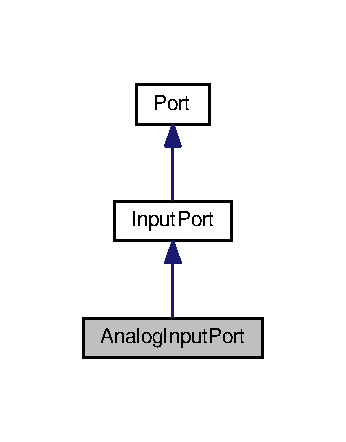
\includegraphics[width=166pt]{classAnalogInputPort__inherit__graph}
\end{center}
\end{figure}


Collaboration diagram for Analog\+Input\+Port\+:\nopagebreak
\begin{figure}[H]
\begin{center}
\leavevmode
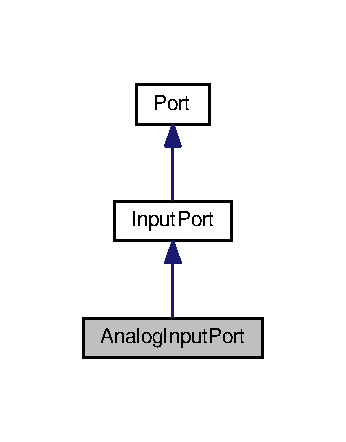
\includegraphics[width=166pt]{classAnalogInputPort__coll__graph}
\end{center}
\end{figure}
\subsection*{Public Member Functions}
\begin{DoxyCompactItemize}
\item 
double \hyperlink{classAnalogInputPort_a7668c7a5ff22d7e75f3ac939070b7dad}{read} ()
\item 
\hyperlink{classAnalogInputPort_add5dffb9783add017bbbf7fa925a6ae5}{Analog\+Input\+Port} (unsigned int pin, unsigned int resolution\+\_\+bits)
\item 
virtual \hyperlink{classAnalogInputPort_ae777b781d7358b1eb6eaf859aebecb84}{$\sim$\+Analog\+Input\+Port} ()
\end{DoxyCompactItemize}
\subsection*{Additional Inherited Members}


\subsection{Constructor \& Destructor Documentation}
\index{Analog\+Input\+Port@{Analog\+Input\+Port}!Analog\+Input\+Port@{Analog\+Input\+Port}}
\index{Analog\+Input\+Port@{Analog\+Input\+Port}!Analog\+Input\+Port@{Analog\+Input\+Port}}
\subsubsection[{\texorpdfstring{Analog\+Input\+Port(unsigned int pin, unsigned int resolution\+\_\+bits)}{AnalogInputPort(unsigned int pin, unsigned int resolution_bits)}}]{\setlength{\rightskip}{0pt plus 5cm}Analog\+Input\+Port\+::\+Analog\+Input\+Port (
\begin{DoxyParamCaption}
\item[{unsigned int}]{pin, }
\item[{unsigned int}]{resolution\+\_\+bits}
\end{DoxyParamCaption}
)}\hypertarget{classAnalogInputPort_add5dffb9783add017bbbf7fa925a6ae5}{}\label{classAnalogInputPort_add5dffb9783add017bbbf7fa925a6ae5}
\index{Analog\+Input\+Port@{Analog\+Input\+Port}!````~Analog\+Input\+Port@{$\sim$\+Analog\+Input\+Port}}
\index{````~Analog\+Input\+Port@{$\sim$\+Analog\+Input\+Port}!Analog\+Input\+Port@{Analog\+Input\+Port}}
\subsubsection[{\texorpdfstring{$\sim$\+Analog\+Input\+Port()}{~AnalogInputPort()}}]{\setlength{\rightskip}{0pt plus 5cm}Analog\+Input\+Port\+::$\sim$\+Analog\+Input\+Port (
\begin{DoxyParamCaption}
{}
\end{DoxyParamCaption}
)\hspace{0.3cm}{\ttfamily [virtual]}}\hypertarget{classAnalogInputPort_ae777b781d7358b1eb6eaf859aebecb84}{}\label{classAnalogInputPort_ae777b781d7358b1eb6eaf859aebecb84}


\subsection{Member Function Documentation}
\index{Analog\+Input\+Port@{Analog\+Input\+Port}!read@{read}}
\index{read@{read}!Analog\+Input\+Port@{Analog\+Input\+Port}}
\subsubsection[{\texorpdfstring{read()}{read()}}]{\setlength{\rightskip}{0pt plus 5cm}double Analog\+Input\+Port\+::read (
\begin{DoxyParamCaption}
{}
\end{DoxyParamCaption}
)\hspace{0.3cm}{\ttfamily [virtual]}}\hypertarget{classAnalogInputPort_a7668c7a5ff22d7e75f3ac939070b7dad}{}\label{classAnalogInputPort_a7668c7a5ff22d7e75f3ac939070b7dad}


Implements \hyperlink{classInputPort_a0dd029736ef41eaf5c1b079c3b8d4ba3}{Input\+Port}.



The documentation for this class was generated from the following files\+:\begin{DoxyCompactItemize}
\item 
\hyperlink{Port_8hpp}{Port.\+hpp}\item 
\hyperlink{Port_8cpp}{Port.\+cpp}\end{DoxyCompactItemize}

\hypertarget{classAnalogOutputPort}{}\section{Analog\+Output\+Port Class Reference}
\label{classAnalogOutputPort}\index{Analog\+Output\+Port@{Analog\+Output\+Port}}


{\ttfamily \#include $<$Port.\+hpp$>$}



Inheritance diagram for Analog\+Output\+Port\+:\nopagebreak
\begin{figure}[H]
\begin{center}
\leavevmode
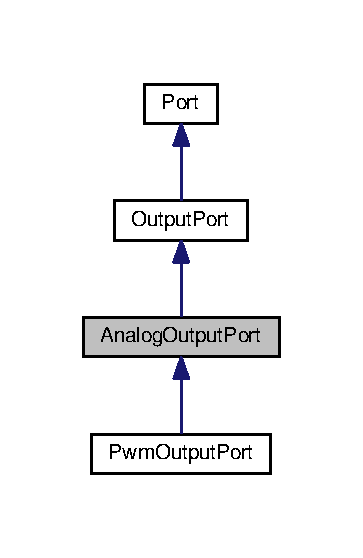
\includegraphics[width=174pt]{classAnalogOutputPort__inherit__graph}
\end{center}
\end{figure}


Collaboration diagram for Analog\+Output\+Port\+:\nopagebreak
\begin{figure}[H]
\begin{center}
\leavevmode
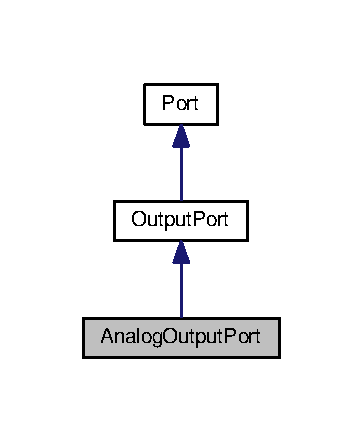
\includegraphics[width=174pt]{classAnalogOutputPort__coll__graph}
\end{center}
\end{figure}
\subsection*{Public Member Functions}
\begin{DoxyCompactItemize}
\item 
void \hyperlink{classAnalogOutputPort_a19f3b98d37462406123232c16a3d96fc}{write} (double value)
\item 
\hyperlink{classAnalogOutputPort_a4968d6d0cee687bc4c072f7dde27aa4b}{Analog\+Output\+Port} (unsigned int pin, unsigned int bit\+\_\+resolution)
\item 
virtual \hyperlink{classAnalogOutputPort_a502e0d648a9b671eb46c5571eb36918a}{$\sim$\+Analog\+Output\+Port} ()
\end{DoxyCompactItemize}
\subsection*{Additional Inherited Members}


\subsection{Constructor \& Destructor Documentation}
\index{Analog\+Output\+Port@{Analog\+Output\+Port}!Analog\+Output\+Port@{Analog\+Output\+Port}}
\index{Analog\+Output\+Port@{Analog\+Output\+Port}!Analog\+Output\+Port@{Analog\+Output\+Port}}
\subsubsection[{\texorpdfstring{Analog\+Output\+Port(unsigned int pin, unsigned int bit\+\_\+resolution)}{AnalogOutputPort(unsigned int pin, unsigned int bit_resolution)}}]{\setlength{\rightskip}{0pt plus 5cm}Analog\+Output\+Port\+::\+Analog\+Output\+Port (
\begin{DoxyParamCaption}
\item[{unsigned int}]{pin, }
\item[{unsigned int}]{bit\+\_\+resolution}
\end{DoxyParamCaption}
)}\hypertarget{classAnalogOutputPort_a4968d6d0cee687bc4c072f7dde27aa4b}{}\label{classAnalogOutputPort_a4968d6d0cee687bc4c072f7dde27aa4b}
\index{Analog\+Output\+Port@{Analog\+Output\+Port}!````~Analog\+Output\+Port@{$\sim$\+Analog\+Output\+Port}}
\index{````~Analog\+Output\+Port@{$\sim$\+Analog\+Output\+Port}!Analog\+Output\+Port@{Analog\+Output\+Port}}
\subsubsection[{\texorpdfstring{$\sim$\+Analog\+Output\+Port()}{~AnalogOutputPort()}}]{\setlength{\rightskip}{0pt plus 5cm}Analog\+Output\+Port\+::$\sim$\+Analog\+Output\+Port (
\begin{DoxyParamCaption}
{}
\end{DoxyParamCaption}
)\hspace{0.3cm}{\ttfamily [virtual]}}\hypertarget{classAnalogOutputPort_a502e0d648a9b671eb46c5571eb36918a}{}\label{classAnalogOutputPort_a502e0d648a9b671eb46c5571eb36918a}


\subsection{Member Function Documentation}
\index{Analog\+Output\+Port@{Analog\+Output\+Port}!write@{write}}
\index{write@{write}!Analog\+Output\+Port@{Analog\+Output\+Port}}
\subsubsection[{\texorpdfstring{write(double value)}{write(double value)}}]{\setlength{\rightskip}{0pt plus 5cm}void Analog\+Output\+Port\+::write (
\begin{DoxyParamCaption}
\item[{double}]{value}
\end{DoxyParamCaption}
)\hspace{0.3cm}{\ttfamily [virtual]}}\hypertarget{classAnalogOutputPort_a19f3b98d37462406123232c16a3d96fc}{}\label{classAnalogOutputPort_a19f3b98d37462406123232c16a3d96fc}


Implements \hyperlink{classOutputPort_a36ab0474c09692287507ddb783671566}{Output\+Port}.



Reimplemented in \hyperlink{classPwmOutputPort_a948d48c45f080e74931ac35b9f1fe31b}{Pwm\+Output\+Port}.



The documentation for this class was generated from the following files\+:\begin{DoxyCompactItemize}
\item 
\hyperlink{Port_8hpp}{Port.\+hpp}\item 
\hyperlink{Port_8cpp}{Port.\+cpp}\end{DoxyCompactItemize}

\hypertarget{classArduinoPortFactory}{}\section{Arduino\+Port\+Factory Class Reference}
\label{classArduinoPortFactory}\index{Arduino\+Port\+Factory@{Arduino\+Port\+Factory}}


{\ttfamily \#include $<$Port.\+hpp$>$}



Inheritance diagram for Arduino\+Port\+Factory\+:\nopagebreak
\begin{figure}[H]
\begin{center}
\leavevmode
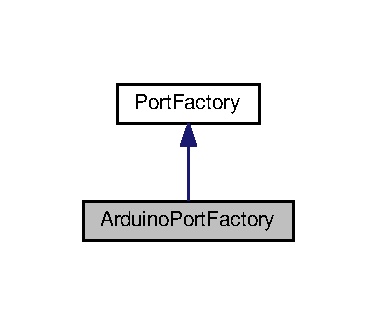
\includegraphics[width=181pt]{classArduinoPortFactory__inherit__graph}
\end{center}
\end{figure}


Collaboration diagram for Arduino\+Port\+Factory\+:\nopagebreak
\begin{figure}[H]
\begin{center}
\leavevmode
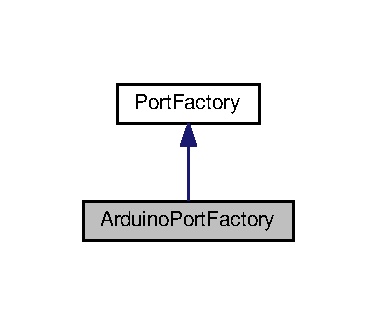
\includegraphics[width=181pt]{classArduinoPortFactory__coll__graph}
\end{center}
\end{figure}
\subsection*{Additional Inherited Members}


The documentation for this class was generated from the following files\+:\begin{DoxyCompactItemize}
\item 
\hyperlink{Port_8hpp}{Port.\+hpp}\item 
\hyperlink{Port_8cpp}{Port.\+cpp}\end{DoxyCompactItemize}

\hypertarget{classAreaIDSelect}{}\section{Area\+I\+D\+Select Class Reference}
\label{classAreaIDSelect}\index{Area\+I\+D\+Select@{Area\+I\+D\+Select}}


{\ttfamily \#include $<$Joint\+Select.\+hpp$>$}

\subsection*{Static Public Attributes}
\begin{DoxyCompactItemize}
\item 
static const \hyperlink{JointSelect_8hpp_a0b0b6279ef5d4a446f8f07404dc868d3}{Area\+ID} \hyperlink{classAreaIDSelect_a4df58116b3d3e37c36782251a507c81f}{L\+E\+F\+T\+\_\+\+L\+EG} = 0
\item 
static const \hyperlink{JointSelect_8hpp_a0b0b6279ef5d4a446f8f07404dc868d3}{Area\+ID} \hyperlink{classAreaIDSelect_af3ad34b4529935bf925bcc668a351a02}{R\+I\+G\+H\+T\+\_\+\+L\+EG} = 1
\end{DoxyCompactItemize}


\subsection{Member Data Documentation}
\index{Area\+I\+D\+Select@{Area\+I\+D\+Select}!L\+E\+F\+T\+\_\+\+L\+EG@{L\+E\+F\+T\+\_\+\+L\+EG}}
\index{L\+E\+F\+T\+\_\+\+L\+EG@{L\+E\+F\+T\+\_\+\+L\+EG}!Area\+I\+D\+Select@{Area\+I\+D\+Select}}
\subsubsection[{\texorpdfstring{L\+E\+F\+T\+\_\+\+L\+EG}{LEFT_LEG}}]{\setlength{\rightskip}{0pt plus 5cm}const {\bf Area\+ID} Area\+I\+D\+Select\+::\+L\+E\+F\+T\+\_\+\+L\+EG = 0\hspace{0.3cm}{\ttfamily [static]}}\hypertarget{classAreaIDSelect_a4df58116b3d3e37c36782251a507c81f}{}\label{classAreaIDSelect_a4df58116b3d3e37c36782251a507c81f}
\index{Area\+I\+D\+Select@{Area\+I\+D\+Select}!R\+I\+G\+H\+T\+\_\+\+L\+EG@{R\+I\+G\+H\+T\+\_\+\+L\+EG}}
\index{R\+I\+G\+H\+T\+\_\+\+L\+EG@{R\+I\+G\+H\+T\+\_\+\+L\+EG}!Area\+I\+D\+Select@{Area\+I\+D\+Select}}
\subsubsection[{\texorpdfstring{R\+I\+G\+H\+T\+\_\+\+L\+EG}{RIGHT_LEG}}]{\setlength{\rightskip}{0pt plus 5cm}const {\bf Area\+ID} Area\+I\+D\+Select\+::\+R\+I\+G\+H\+T\+\_\+\+L\+EG = 1\hspace{0.3cm}{\ttfamily [static]}}\hypertarget{classAreaIDSelect_af3ad34b4529935bf925bcc668a351a02}{}\label{classAreaIDSelect_af3ad34b4529935bf925bcc668a351a02}


The documentation for this class was generated from the following file\+:\begin{DoxyCompactItemize}
\item 
\hyperlink{JointSelect_8hpp}{Joint\+Select.\+hpp}\end{DoxyCompactItemize}

\hypertarget{classAverage}{}\section{Average Class Reference}
\label{classAverage}\index{Average@{Average}}


{\ttfamily \#include $<$Utils.\+hpp$>$}



Inheritance diagram for Average\+:\nopagebreak
\begin{figure}[H]
\begin{center}
\leavevmode
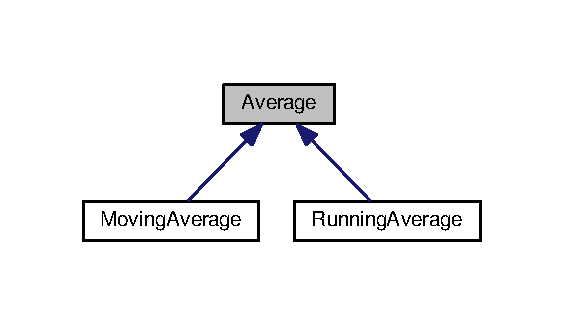
\includegraphics[width=271pt]{classAverage__inherit__graph}
\end{center}
\end{figure}
\subsection*{Public Member Functions}
\begin{DoxyCompactItemize}
\item 
virtual \hyperlink{classAverage_a45844d3a06e8731a089eabe1a31df982}{$\sim$\+Average} ()
\item 
virtual double \hyperlink{classAverage_ac6e6c55dfc9c79e99e781a6b9337ad6f}{update} (double value)=0
\item 
virtual double \hyperlink{classAverage_a1951ea6b4b4c12d21b4a3e358a5e184b}{get\+Average} ()=0
\item 
virtual void \hyperlink{classAverage_aff2ccc3f273b5de81b8cc2ca52b8bc8d}{reset} ()=0
\item 
virtual void \hyperlink{classAverage_ae5c3a77f0792540fbf553c80d075172e}{reset} (double value)=0
\end{DoxyCompactItemize}


\subsection{Constructor \& Destructor Documentation}
\index{Average@{Average}!````~Average@{$\sim$\+Average}}
\index{````~Average@{$\sim$\+Average}!Average@{Average}}
\subsubsection[{\texorpdfstring{$\sim$\+Average()}{~Average()}}]{\setlength{\rightskip}{0pt plus 5cm}Average\+::$\sim$\+Average (
\begin{DoxyParamCaption}
{}
\end{DoxyParamCaption}
)\hspace{0.3cm}{\ttfamily [virtual]}}\hypertarget{classAverage_a45844d3a06e8731a089eabe1a31df982}{}\label{classAverage_a45844d3a06e8731a089eabe1a31df982}


\subsection{Member Function Documentation}
\index{Average@{Average}!get\+Average@{get\+Average}}
\index{get\+Average@{get\+Average}!Average@{Average}}
\subsubsection[{\texorpdfstring{get\+Average()=0}{getAverage()=0}}]{\setlength{\rightskip}{0pt plus 5cm}virtual double Average\+::get\+Average (
\begin{DoxyParamCaption}
{}
\end{DoxyParamCaption}
)\hspace{0.3cm}{\ttfamily [pure virtual]}}\hypertarget{classAverage_a1951ea6b4b4c12d21b4a3e358a5e184b}{}\label{classAverage_a1951ea6b4b4c12d21b4a3e358a5e184b}


Implemented in \hyperlink{classMovingAverage_a7725076484accef33958b5e2ede6f569}{Moving\+Average}, and \hyperlink{classRunningAverage_a8f41fa82e58f9ba4eea9a10a7d9f4c30}{Running\+Average}.

\index{Average@{Average}!reset@{reset}}
\index{reset@{reset}!Average@{Average}}
\subsubsection[{\texorpdfstring{reset()=0}{reset()=0}}]{\setlength{\rightskip}{0pt plus 5cm}virtual void Average\+::reset (
\begin{DoxyParamCaption}
{}
\end{DoxyParamCaption}
)\hspace{0.3cm}{\ttfamily [pure virtual]}}\hypertarget{classAverage_aff2ccc3f273b5de81b8cc2ca52b8bc8d}{}\label{classAverage_aff2ccc3f273b5de81b8cc2ca52b8bc8d}


Implemented in \hyperlink{classMovingAverage_a0f1717f9e279400589743188c0b29e55}{Moving\+Average}, and \hyperlink{classRunningAverage_a0b9429f6d0109bab34879a92adf65a1d}{Running\+Average}.

\index{Average@{Average}!reset@{reset}}
\index{reset@{reset}!Average@{Average}}
\subsubsection[{\texorpdfstring{reset(double value)=0}{reset(double value)=0}}]{\setlength{\rightskip}{0pt plus 5cm}virtual void Average\+::reset (
\begin{DoxyParamCaption}
\item[{double}]{value}
\end{DoxyParamCaption}
)\hspace{0.3cm}{\ttfamily [pure virtual]}}\hypertarget{classAverage_ae5c3a77f0792540fbf553c80d075172e}{}\label{classAverage_ae5c3a77f0792540fbf553c80d075172e}


Implemented in \hyperlink{classMovingAverage_a90028f3da9bb57ba5cebf8eff7df9231}{Moving\+Average}, and \hyperlink{classRunningAverage_a68f538c3216535b5e0387dc82c3c60b9}{Running\+Average}.

\index{Average@{Average}!update@{update}}
\index{update@{update}!Average@{Average}}
\subsubsection[{\texorpdfstring{update(double value)=0}{update(double value)=0}}]{\setlength{\rightskip}{0pt plus 5cm}virtual double Average\+::update (
\begin{DoxyParamCaption}
\item[{double}]{value}
\end{DoxyParamCaption}
)\hspace{0.3cm}{\ttfamily [pure virtual]}}\hypertarget{classAverage_ac6e6c55dfc9c79e99e781a6b9337ad6f}{}\label{classAverage_ac6e6c55dfc9c79e99e781a6b9337ad6f}


Implemented in \hyperlink{classMovingAverage_afd5d70f2d7adcfa086850094f164f473}{Moving\+Average}, and \hyperlink{classRunningAverage_a2e5045095e304ab3b41b1f9559f28385}{Running\+Average}.



The documentation for this class was generated from the following files\+:\begin{DoxyCompactItemize}
\item 
\hyperlink{Utils_8hpp}{Utils.\+hpp}\item 
\hyperlink{Utils_8cpp}{Utils.\+cpp}\end{DoxyCompactItemize}

\hypertarget{classBalanceControl}{}\section{Balance\+Control Class Reference}
\label{classBalanceControl}\index{Balance\+Control@{Balance\+Control}}


{\ttfamily \#include $<$Control\+\_\+\+Algorithms.\+hpp$>$}



Inheritance diagram for Balance\+Control\+:\nopagebreak
\begin{figure}[H]
\begin{center}
\leavevmode
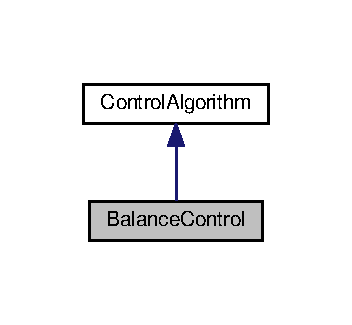
\includegraphics[width=169pt]{classBalanceControl__inherit__graph}
\end{center}
\end{figure}


Collaboration diagram for Balance\+Control\+:
\nopagebreak
\begin{figure}[H]
\begin{center}
\leavevmode
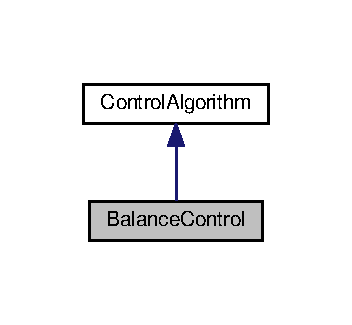
\includegraphics[width=169pt]{classBalanceControl__coll__graph}
\end{center}
\end{figure}
\subsection*{Public Member Functions}
\begin{DoxyCompactItemize}
\item 
\hyperlink{classBalanceControl_ac7ee7f2242e22ec7152fc2c8ff77c6a2}{Balance\+Control} (\hyperlink{States_8hpp_a26aafbeccd8f356b39e1809f1ab9cfdc}{State\+ID} state\+\_\+id)
\item 
double \hyperlink{classBalanceControl_ab7bc00e4dea77cf34c02ef1f4bb2feec}{get\+Setpoint} (\hyperlink{classSensorReport}{Sensor\+Report} $\ast$report)
\item 
\hyperlink{Control__Algorithms_8hpp_afda28772870dd56f60cd7a301337392c}{Control\+Algorithm\+Type} \hyperlink{classBalanceControl_a8314d9b67c800b7e0ca2be07ae7e1343}{get\+Type} ()
\item 
double \hyperlink{classBalanceControl_a0ba1c9cd74a877eb0f748325763c02e4}{get\+Shaping\+Iterations} ()
\item 
bool \hyperlink{classBalanceControl_a9761db9b15bb15e6d2f19f6d2243c888}{use\+Shaping\+Function} ()
\end{DoxyCompactItemize}
\subsection*{Additional Inherited Members}


\subsection{Constructor \& Destructor Documentation}
\index{Balance\+Control@{Balance\+Control}!Balance\+Control@{Balance\+Control}}
\index{Balance\+Control@{Balance\+Control}!Balance\+Control@{Balance\+Control}}
\subsubsection[{\texorpdfstring{Balance\+Control(\+State\+I\+D state\+\_\+id)}{BalanceControl(StateID state_id)}}]{\setlength{\rightskip}{0pt plus 5cm}Balance\+Control\+::\+Balance\+Control (
\begin{DoxyParamCaption}
\item[{{\bf State\+ID}}]{state\+\_\+id}
\end{DoxyParamCaption}
)}\hypertarget{classBalanceControl_ac7ee7f2242e22ec7152fc2c8ff77c6a2}{}\label{classBalanceControl_ac7ee7f2242e22ec7152fc2c8ff77c6a2}


\subsection{Member Function Documentation}
\index{Balance\+Control@{Balance\+Control}!get\+Setpoint@{get\+Setpoint}}
\index{get\+Setpoint@{get\+Setpoint}!Balance\+Control@{Balance\+Control}}
\subsubsection[{\texorpdfstring{get\+Setpoint(\+Sensor\+Report $\ast$report)}{getSetpoint(SensorReport *report)}}]{\setlength{\rightskip}{0pt plus 5cm}double Balance\+Control\+::get\+Setpoint (
\begin{DoxyParamCaption}
\item[{{\bf Sensor\+Report} $\ast$}]{report}
\end{DoxyParamCaption}
)\hspace{0.3cm}{\ttfamily [virtual]}}\hypertarget{classBalanceControl_ab7bc00e4dea77cf34c02ef1f4bb2feec}{}\label{classBalanceControl_ab7bc00e4dea77cf34c02ef1f4bb2feec}


Implements \hyperlink{classControlAlgorithm_a038ebc5f26c3ae460f04eaf7f0dc0e29}{Control\+Algorithm}.

\index{Balance\+Control@{Balance\+Control}!get\+Shaping\+Iterations@{get\+Shaping\+Iterations}}
\index{get\+Shaping\+Iterations@{get\+Shaping\+Iterations}!Balance\+Control@{Balance\+Control}}
\subsubsection[{\texorpdfstring{get\+Shaping\+Iterations()}{getShapingIterations()}}]{\setlength{\rightskip}{0pt plus 5cm}double Balance\+Control\+::get\+Shaping\+Iterations (
\begin{DoxyParamCaption}
{}
\end{DoxyParamCaption}
)\hspace{0.3cm}{\ttfamily [virtual]}}\hypertarget{classBalanceControl_a0ba1c9cd74a877eb0f748325763c02e4}{}\label{classBalanceControl_a0ba1c9cd74a877eb0f748325763c02e4}


Reimplemented from \hyperlink{classControlAlgorithm_a5fd58cfd5b601dc4556170bb620ea7f5}{Control\+Algorithm}.

\index{Balance\+Control@{Balance\+Control}!get\+Type@{get\+Type}}
\index{get\+Type@{get\+Type}!Balance\+Control@{Balance\+Control}}
\subsubsection[{\texorpdfstring{get\+Type()}{getType()}}]{\setlength{\rightskip}{0pt plus 5cm}{\bf Control\+Algorithm\+Type} Balance\+Control\+::get\+Type (
\begin{DoxyParamCaption}
{}
\end{DoxyParamCaption}
)\hspace{0.3cm}{\ttfamily [virtual]}}\hypertarget{classBalanceControl_a8314d9b67c800b7e0ca2be07ae7e1343}{}\label{classBalanceControl_a8314d9b67c800b7e0ca2be07ae7e1343}


Implements \hyperlink{classControlAlgorithm_a432f51282dfe836befccdecaaa9741c5}{Control\+Algorithm}.

\index{Balance\+Control@{Balance\+Control}!use\+Shaping\+Function@{use\+Shaping\+Function}}
\index{use\+Shaping\+Function@{use\+Shaping\+Function}!Balance\+Control@{Balance\+Control}}
\subsubsection[{\texorpdfstring{use\+Shaping\+Function()}{useShapingFunction()}}]{\setlength{\rightskip}{0pt plus 5cm}bool Balance\+Control\+::use\+Shaping\+Function (
\begin{DoxyParamCaption}
{}
\end{DoxyParamCaption}
)\hspace{0.3cm}{\ttfamily [virtual]}}\hypertarget{classBalanceControl_a9761db9b15bb15e6d2f19f6d2243c888}{}\label{classBalanceControl_a9761db9b15bb15e6d2f19f6d2243c888}


Implements \hyperlink{classControlAlgorithm_ac9e2b1e3677e4ace7071c540fe035ae4}{Control\+Algorithm}.



The documentation for this class was generated from the following files\+:\begin{DoxyCompactItemize}
\item 
\hyperlink{Control__Algorithms_8hpp}{Control\+\_\+\+Algorithms.\+hpp}\item 
\hyperlink{Control__Algorithms_8cpp}{Control\+\_\+\+Algorithms.\+cpp}\end{DoxyCompactItemize}

\hypertarget{classBangBangControl}{}\section{Bang\+Bang\+Control Class Reference}
\label{classBangBangControl}\index{Bang\+Bang\+Control@{Bang\+Bang\+Control}}


{\ttfamily \#include $<$Control\+\_\+\+Algorithms.\+hpp$>$}



Inheritance diagram for Bang\+Bang\+Control\+:\nopagebreak
\begin{figure}[H]
\begin{center}
\leavevmode
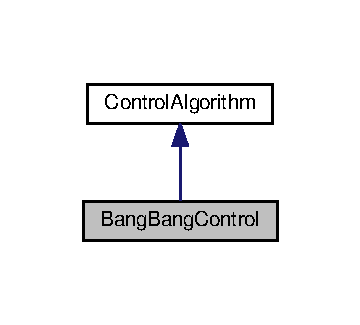
\includegraphics[width=173pt]{classBangBangControl__inherit__graph}
\end{center}
\end{figure}


Collaboration diagram for Bang\+Bang\+Control\+:
\nopagebreak
\begin{figure}[H]
\begin{center}
\leavevmode
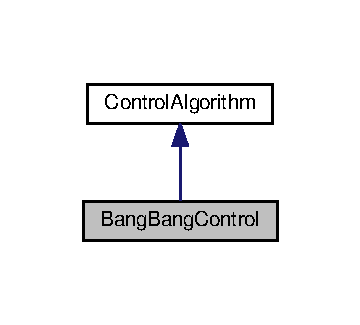
\includegraphics[width=173pt]{classBangBangControl__coll__graph}
\end{center}
\end{figure}
\subsection*{Public Member Functions}
\begin{DoxyCompactItemize}
\item 
\hyperlink{classBangBangControl_a0b0353ef64816c09b321af53a315975d}{Bang\+Bang\+Control} (\hyperlink{States_8hpp_a26aafbeccd8f356b39e1809f1ab9cfdc}{State\+ID} state\+\_\+id)
\item 
double \hyperlink{classBangBangControl_a6fd492fbf7d9e255ef82c85f426cb794}{get\+Setpoint} (\hyperlink{classSensorReport}{Sensor\+Report} $\ast$report)
\item 
\hyperlink{Control__Algorithms_8hpp_afda28772870dd56f60cd7a301337392c}{Control\+Algorithm\+Type} \hyperlink{classBangBangControl_a240b1a40e88fdcd4e943319dd83654d0}{get\+Type} ()
\item 
bool \hyperlink{classBangBangControl_af85b04c727a5e11c1d54d0a15d5ca64c}{use\+Shaping\+Function} ()
\item 
void \hyperlink{classBangBangControl_a9e8e9d63842c9640212993f8ba02e4a1}{activate} ()
\end{DoxyCompactItemize}
\subsection*{Additional Inherited Members}


\subsection{Constructor \& Destructor Documentation}
\index{Bang\+Bang\+Control@{Bang\+Bang\+Control}!Bang\+Bang\+Control@{Bang\+Bang\+Control}}
\index{Bang\+Bang\+Control@{Bang\+Bang\+Control}!Bang\+Bang\+Control@{Bang\+Bang\+Control}}
\subsubsection[{\texorpdfstring{Bang\+Bang\+Control(\+State\+I\+D state\+\_\+id)}{BangBangControl(StateID state_id)}}]{\setlength{\rightskip}{0pt plus 5cm}Bang\+Bang\+Control\+::\+Bang\+Bang\+Control (
\begin{DoxyParamCaption}
\item[{{\bf State\+ID}}]{state\+\_\+id}
\end{DoxyParamCaption}
)}\hypertarget{classBangBangControl_a0b0353ef64816c09b321af53a315975d}{}\label{classBangBangControl_a0b0353ef64816c09b321af53a315975d}


\subsection{Member Function Documentation}
\index{Bang\+Bang\+Control@{Bang\+Bang\+Control}!activate@{activate}}
\index{activate@{activate}!Bang\+Bang\+Control@{Bang\+Bang\+Control}}
\subsubsection[{\texorpdfstring{activate()}{activate()}}]{\setlength{\rightskip}{0pt plus 5cm}void Bang\+Bang\+Control\+::activate (
\begin{DoxyParamCaption}
{}
\end{DoxyParamCaption}
)\hspace{0.3cm}{\ttfamily [virtual]}}\hypertarget{classBangBangControl_a9e8e9d63842c9640212993f8ba02e4a1}{}\label{classBangBangControl_a9e8e9d63842c9640212993f8ba02e4a1}


Reimplemented from \hyperlink{classControlAlgorithm_a0da6d49c48afb6df7c1bc4bad4e5a3f0}{Control\+Algorithm}.

\index{Bang\+Bang\+Control@{Bang\+Bang\+Control}!get\+Setpoint@{get\+Setpoint}}
\index{get\+Setpoint@{get\+Setpoint}!Bang\+Bang\+Control@{Bang\+Bang\+Control}}
\subsubsection[{\texorpdfstring{get\+Setpoint(\+Sensor\+Report $\ast$report)}{getSetpoint(SensorReport *report)}}]{\setlength{\rightskip}{0pt plus 5cm}double Bang\+Bang\+Control\+::get\+Setpoint (
\begin{DoxyParamCaption}
\item[{{\bf Sensor\+Report} $\ast$}]{report}
\end{DoxyParamCaption}
)\hspace{0.3cm}{\ttfamily [virtual]}}\hypertarget{classBangBangControl_a6fd492fbf7d9e255ef82c85f426cb794}{}\label{classBangBangControl_a6fd492fbf7d9e255ef82c85f426cb794}


Implements \hyperlink{classControlAlgorithm_a038ebc5f26c3ae460f04eaf7f0dc0e29}{Control\+Algorithm}.

\index{Bang\+Bang\+Control@{Bang\+Bang\+Control}!get\+Type@{get\+Type}}
\index{get\+Type@{get\+Type}!Bang\+Bang\+Control@{Bang\+Bang\+Control}}
\subsubsection[{\texorpdfstring{get\+Type()}{getType()}}]{\setlength{\rightskip}{0pt plus 5cm}{\bf Control\+Algorithm\+Type} Bang\+Bang\+Control\+::get\+Type (
\begin{DoxyParamCaption}
{}
\end{DoxyParamCaption}
)\hspace{0.3cm}{\ttfamily [virtual]}}\hypertarget{classBangBangControl_a240b1a40e88fdcd4e943319dd83654d0}{}\label{classBangBangControl_a240b1a40e88fdcd4e943319dd83654d0}


Implements \hyperlink{classControlAlgorithm_a432f51282dfe836befccdecaaa9741c5}{Control\+Algorithm}.

\index{Bang\+Bang\+Control@{Bang\+Bang\+Control}!use\+Shaping\+Function@{use\+Shaping\+Function}}
\index{use\+Shaping\+Function@{use\+Shaping\+Function}!Bang\+Bang\+Control@{Bang\+Bang\+Control}}
\subsubsection[{\texorpdfstring{use\+Shaping\+Function()}{useShapingFunction()}}]{\setlength{\rightskip}{0pt plus 5cm}bool Bang\+Bang\+Control\+::use\+Shaping\+Function (
\begin{DoxyParamCaption}
{}
\end{DoxyParamCaption}
)\hspace{0.3cm}{\ttfamily [virtual]}}\hypertarget{classBangBangControl_af85b04c727a5e11c1d54d0a15d5ca64c}{}\label{classBangBangControl_af85b04c727a5e11c1d54d0a15d5ca64c}


Implements \hyperlink{classControlAlgorithm_ac9e2b1e3677e4ace7071c540fe035ae4}{Control\+Algorithm}.



The documentation for this class was generated from the following files\+:\begin{DoxyCompactItemize}
\item 
\hyperlink{Control__Algorithms_8hpp}{Control\+\_\+\+Algorithms.\+hpp}\item 
\hyperlink{Control__Algorithms_8cpp}{Control\+\_\+\+Algorithms.\+cpp}\end{DoxyCompactItemize}

\hypertarget{classBoard}{}\section{Board Class Reference}
\label{classBoard}\index{Board@{Board}}


{\ttfamily \#include $<$Board.\+hpp$>$}

\subsection*{Public Member Functions}
\begin{DoxyCompactItemize}
\item 
\hyperlink{classBoard_a9ee491d4fea680cf69b033374a9fdfcb}{Board} ()
\item 
\hyperlink{classBoard_af73f45730119a1fd8f6670f53f959e68}{$\sim$\+Board} ()
\item 
void \hyperlink{classBoard_a022ee938df244ab52f8ce4c3541a7600}{turn\+On\+Led} ()
\item 
\hyperlink{classTxPort}{Tx\+Port} $\ast$ \hyperlink{classBoard_a4d2aeef1855a94949426a0004da0d206}{take\+Bluetooth\+Tx\+Port} ()
\item 
\hyperlink{classRxPort}{Rx\+Port} $\ast$ \hyperlink{classBoard_a3b0eb16b49af6cecd2615ddebb301a83}{take\+Bluetooth\+Rx\+Port} ()
\item 
\hyperlink{classInputPort}{Input\+Port} $\ast$ \hyperlink{classBoard_af30a08ff2ff3e86e290d8c512907a422}{take\+Fsr\+Sense\+Left\+Toe\+Port} ()
\item 
\hyperlink{classInputPort}{Input\+Port} $\ast$ \hyperlink{classBoard_a21da1fccb5bb27ade658cbfdf05a64f9}{take\+Fsr\+Sense\+Left\+Heel\+Port} ()
\item 
\hyperlink{classInputPort}{Input\+Port} $\ast$ \hyperlink{classBoard_a78a9a73532be37ed05d6d2f12e5b7182}{take\+Fsr\+Sense\+Right\+Toe\+Port} ()
\item 
\hyperlink{classInputPort}{Input\+Port} $\ast$ \hyperlink{classBoard_acea5ca8cba177d604319585260afb1b8}{take\+Fsr\+Sense\+Right\+Heel\+Port} ()
\item 
\hyperlink{classInputPort}{Input\+Port} $\ast$ \hyperlink{classBoard_a77deee0229cdc90dfba844f733738548}{take\+Torque\+Sensor\+Left\+Knee\+Port} ()
\item 
\hyperlink{classInputPort}{Input\+Port} $\ast$ \hyperlink{classBoard_a4a3194002b85e3adea633d849964ce54}{take\+Torque\+Sensor\+Left\+Ankle\+Port} ()
\item 
\hyperlink{classInputPort}{Input\+Port} $\ast$ \hyperlink{classBoard_a425a898e1ebbf15cbb9198f723d8279b}{take\+Torque\+Sensor\+Right\+Knee\+Port} ()
\item 
\hyperlink{classInputPort}{Input\+Port} $\ast$ \hyperlink{classBoard_a2728251277213d1d3b51adc60d57c88c}{take\+Torque\+Sensor\+Right\+Ankle\+Port} ()
\item 
\hyperlink{classOutputPort}{Output\+Port} $\ast$ \hyperlink{classBoard_ae11de17a46428a72a2596b0b462193ee}{take\+Motor\+Left\+Knee\+Port} ()
\item 
\hyperlink{classOutputPort}{Output\+Port} $\ast$ \hyperlink{classBoard_a7185650a74ca6795c38bf66e6acb0d71}{take\+Motor\+Left\+Ankle\+Port} ()
\item 
\hyperlink{classOutputPort}{Output\+Port} $\ast$ \hyperlink{classBoard_af96d2b8c37435f2b0430238cdfabaf13}{take\+Motor\+Right\+Knee\+Port} ()
\item 
\hyperlink{classOutputPort}{Output\+Port} $\ast$ \hyperlink{classBoard_aa54cf724971416290d50e807b0afbc19}{take\+Motor\+Right\+Ankle\+Port} ()
\item 
\hyperlink{classOutputPort}{Output\+Port} $\ast$ \hyperlink{classBoard_a7771c3fc5e365b4a8f2c3db312792f5a}{take\+Led\+Port} ()
\item 
\hyperlink{classOutputPort}{Output\+Port} $\ast$ \hyperlink{classBoard_a4ec97cefdf203ed9fcafddd098bd194f}{take\+Motor\+Enable\+Port} ()
\item 
\hyperlink{classInputPort}{Input\+Port} $\ast$ \hyperlink{classBoard_a55d3bf54fbec7225b507f44e7826a6d1}{take\+Motor\+Error\+Left\+Knee\+Port} ()
\item 
\hyperlink{classInputPort}{Input\+Port} $\ast$ \hyperlink{classBoard_a40da12d162a16f92111525007e28abd5}{take\+Motor\+Error\+Left\+Ankle\+Port} ()
\item 
\hyperlink{classInputPort}{Input\+Port} $\ast$ \hyperlink{classBoard_ac70e1db27663c5b2f55a744d55846b55}{take\+Motor\+Error\+Right\+Knee\+Port} ()
\item 
\hyperlink{classInputPort}{Input\+Port} $\ast$ \hyperlink{classBoard_affcf61ded54f8e2149c014b6147c0bd0}{take\+Motor\+Error\+Right\+Ankle\+Port} ()
\item 
\hyperlink{classInputPort}{Input\+Port} $\ast$ \hyperlink{classBoard_a625f45733819f5e144bceb61ce886831}{take\+Pot\+Left\+Knee\+Port} ()
\item 
\hyperlink{classInputPort}{Input\+Port} $\ast$ \hyperlink{classBoard_a25d4d7b2a40147c681f1bd50c1037557}{take\+Pot\+Right\+Knee\+Port} ()
\item 
\hyperlink{classInputPort}{Input\+Port} $\ast$ \hyperlink{classBoard_a654483cd7d4d93b768d1b8eb981fbff2}{take\+Pot\+Left\+Ankle\+Port} ()
\item 
\hyperlink{classInputPort}{Input\+Port} $\ast$ \hyperlink{classBoard_ad580a6bc7986156eeb69ea50a02f1563}{take\+Pot\+Right\+Ankle\+Port} ()
\item 
\hyperlink{classImuPort}{Imu\+Port} $\ast$ \hyperlink{classBoard_a732e8cf1e3d1242b89c1f1409131c980}{get\+Imu\+Slot0} ()
\item 
\hyperlink{classImuPort}{Imu\+Port} $\ast$ \hyperlink{classBoard_af5f81580ae8f615858fb5cdb74d9f494}{get\+Imu\+Slot1} ()
\item 
\hyperlink{classImuPort}{Imu\+Port} $\ast$ \hyperlink{classBoard_a84c16ed6f01fd9075f2f393598df2962}{get\+Imu\+Slot2} ()
\item 
int \hyperlink{classBoard_a8ac6af90e1b7c3747dec6a2717e4e0c9}{get\+Imu\+Address0} ()
\item 
int \hyperlink{classBoard_a2a5914d7897e0e293a6c270e35a8d770}{get\+Imu\+Address1} ()
\item 
void \hyperlink{classBoard_a2dadb15f722d1b1e5326fb016dc5af60}{set\+Bluetooth\+Tx\+Port} (\hyperlink{classTxPort}{Tx\+Port} $\ast$port)
\item 
void \hyperlink{classBoard_aa8f470af0dabf15e8208a8a85f3bfdb6}{set\+Bluetooth\+Rx\+Port} (\hyperlink{classRxPort}{Rx\+Port} $\ast$port)
\item 
void \hyperlink{classBoard_a8c0e8c5827e4119797c421df8374b493}{set\+Fsr\+Sense\+Left\+Toe\+Port} (\hyperlink{classInputPort}{Input\+Port} $\ast$port)
\item 
void \hyperlink{classBoard_a5ec129c18aaf991f8f94e981f13a4905}{set\+Fsr\+Sense\+Left\+Heel\+Port} (\hyperlink{classInputPort}{Input\+Port} $\ast$port)
\item 
void \hyperlink{classBoard_aad8cd688c1c492c767d8c7e795344389}{set\+Fsr\+Sense\+Right\+Toe\+Port} (\hyperlink{classInputPort}{Input\+Port} $\ast$port)
\item 
void \hyperlink{classBoard_a303a71aa15a467f0ffea207e6621b8cd}{set\+Fsr\+Sense\+Right\+Heel\+Port} (\hyperlink{classInputPort}{Input\+Port} $\ast$port)
\item 
void \hyperlink{classBoard_ae45adf7a5640338344156fdd32822178}{set\+Torque\+Sensor\+Left\+Knee\+Port} (\hyperlink{classInputPort}{Input\+Port} $\ast$port)
\item 
void \hyperlink{classBoard_af667f98775160ebdbc4cc8ee31cbe910}{set\+Torque\+Sensor\+Left\+Ankle\+Port} (\hyperlink{classInputPort}{Input\+Port} $\ast$port)
\item 
void \hyperlink{classBoard_a8a4b37dc0833c39a644b99f3edd16b9f}{set\+Torque\+Sensor\+Right\+Knee\+Port} (\hyperlink{classInputPort}{Input\+Port} $\ast$port)
\item 
void \hyperlink{classBoard_a269e4e67787dc9e27d472e5c88f0fe83}{set\+Torque\+Sensor\+Right\+Ankle\+Port} (\hyperlink{classInputPort}{Input\+Port} $\ast$port)
\item 
void \hyperlink{classBoard_a480facbc78ceaec928897e80be948977}{set\+Motor\+Left\+Knee\+Port} (\hyperlink{classOutputPort}{Output\+Port} $\ast$port)
\item 
void \hyperlink{classBoard_aebeebf46653c0d1009fd0129ba65c2a0}{set\+Motor\+Left\+Ankle\+Port} (\hyperlink{classOutputPort}{Output\+Port} $\ast$port)
\item 
void \hyperlink{classBoard_acdb5c2acbf9de0d43b06558d0b4cd5f1}{set\+Motor\+Right\+Knee\+Port} (\hyperlink{classOutputPort}{Output\+Port} $\ast$port)
\item 
void \hyperlink{classBoard_a0f1b706acf8d29f207773f1d922946b8}{set\+Motor\+Right\+Ankle\+Port} (\hyperlink{classOutputPort}{Output\+Port} $\ast$port)
\item 
void \hyperlink{classBoard_aeb8a60226ae21067632c011dd339b76c}{set\+Led\+Port} (\hyperlink{classOutputPort}{Output\+Port} $\ast$port)
\item 
void \hyperlink{classBoard_ac3bb78d67ffca86fd4c780308d327e45}{set\+Motor\+Enable\+Port} (\hyperlink{classOutputPort}{Output\+Port} $\ast$port)
\item 
void \hyperlink{classBoard_ab36460d8e4b01128ff0060261b086577}{set\+Motor\+Error\+Left\+Knee\+Port} (\hyperlink{classInputPort}{Input\+Port} $\ast$port)
\item 
void \hyperlink{classBoard_acdec893b7034bd0175980a6b31c7c611}{set\+Motor\+Error\+Left\+Ankle\+Port} (\hyperlink{classInputPort}{Input\+Port} $\ast$port)
\item 
void \hyperlink{classBoard_a944f77aeca71cc0c6afb06355222f01c}{set\+Motor\+Error\+Right\+Knee\+Port} (\hyperlink{classInputPort}{Input\+Port} $\ast$port)
\item 
void \hyperlink{classBoard_a703739a87f21444992922b328710f04c}{set\+Motor\+Error\+Right\+Ankle\+Port} (\hyperlink{classInputPort}{Input\+Port} $\ast$port)
\item 
void \hyperlink{classBoard_a7016b22924417ccfb6a1932bdd8fc78f}{set\+Pot\+Left\+Knee\+Port} (\hyperlink{classInputPort}{Input\+Port} $\ast$port)
\item 
void \hyperlink{classBoard_ad5ad3dc269c1c2f22e1d22e2f69daefc}{set\+Pot\+Right\+Knee\+Port} (\hyperlink{classInputPort}{Input\+Port} $\ast$port)
\item 
void \hyperlink{classBoard_ad79af5f3ce4dd29f53127e5b27aa11be}{set\+Pot\+Left\+Ankle\+Port} (\hyperlink{classInputPort}{Input\+Port} $\ast$port)
\item 
void \hyperlink{classBoard_a2df5ecd2411c91091b123058f795f7e7}{set\+Pot\+Right\+Ankle\+Port} (\hyperlink{classInputPort}{Input\+Port} $\ast$port)
\item 
void \hyperlink{classBoard_ae7d85b5fac2f08847c82f5a649e92b4e}{set\+Imu\+Slot0} (\hyperlink{classImuPort}{Imu\+Port} $\ast$port)
\item 
void \hyperlink{classBoard_a8393ced57177fe471ec4676890e3bfef}{set\+Imu\+Slot1} (\hyperlink{classImuPort}{Imu\+Port} $\ast$port)
\item 
void \hyperlink{classBoard_aff8ad143ff3c31ebffbdb0a38c613724}{set\+Imu\+Slot2} (\hyperlink{classImuPort}{Imu\+Port} $\ast$port)
\item 
void \hyperlink{classBoard_ad19db66886ca758ef9b3dd4a799d3563}{set\+Imu\+Address0} (int address)
\item 
void \hyperlink{classBoard_ad7b736a0dc2a01833b0caecbc272b7fa}{set\+Imu\+Address1} (int address)
\end{DoxyCompactItemize}


\subsection{Constructor \& Destructor Documentation}
\index{Board@{Board}!Board@{Board}}
\index{Board@{Board}!Board@{Board}}
\subsubsection[{\texorpdfstring{Board()}{Board()}}]{\setlength{\rightskip}{0pt plus 5cm}Board\+::\+Board (
\begin{DoxyParamCaption}
{}
\end{DoxyParamCaption}
)}\hypertarget{classBoard_a9ee491d4fea680cf69b033374a9fdfcb}{}\label{classBoard_a9ee491d4fea680cf69b033374a9fdfcb}
\index{Board@{Board}!````~Board@{$\sim$\+Board}}
\index{````~Board@{$\sim$\+Board}!Board@{Board}}
\subsubsection[{\texorpdfstring{$\sim$\+Board()}{~Board()}}]{\setlength{\rightskip}{0pt plus 5cm}Board\+::$\sim$\+Board (
\begin{DoxyParamCaption}
{}
\end{DoxyParamCaption}
)}\hypertarget{classBoard_af73f45730119a1fd8f6670f53f959e68}{}\label{classBoard_af73f45730119a1fd8f6670f53f959e68}


\subsection{Member Function Documentation}
\index{Board@{Board}!get\+Imu\+Address0@{get\+Imu\+Address0}}
\index{get\+Imu\+Address0@{get\+Imu\+Address0}!Board@{Board}}
\subsubsection[{\texorpdfstring{get\+Imu\+Address0()}{getImuAddress0()}}]{\setlength{\rightskip}{0pt plus 5cm}int Board\+::get\+Imu\+Address0 (
\begin{DoxyParamCaption}
{}
\end{DoxyParamCaption}
)}\hypertarget{classBoard_a8ac6af90e1b7c3747dec6a2717e4e0c9}{}\label{classBoard_a8ac6af90e1b7c3747dec6a2717e4e0c9}
\index{Board@{Board}!get\+Imu\+Address1@{get\+Imu\+Address1}}
\index{get\+Imu\+Address1@{get\+Imu\+Address1}!Board@{Board}}
\subsubsection[{\texorpdfstring{get\+Imu\+Address1()}{getImuAddress1()}}]{\setlength{\rightskip}{0pt plus 5cm}int Board\+::get\+Imu\+Address1 (
\begin{DoxyParamCaption}
{}
\end{DoxyParamCaption}
)}\hypertarget{classBoard_a2a5914d7897e0e293a6c270e35a8d770}{}\label{classBoard_a2a5914d7897e0e293a6c270e35a8d770}
\index{Board@{Board}!get\+Imu\+Slot0@{get\+Imu\+Slot0}}
\index{get\+Imu\+Slot0@{get\+Imu\+Slot0}!Board@{Board}}
\subsubsection[{\texorpdfstring{get\+Imu\+Slot0()}{getImuSlot0()}}]{\setlength{\rightskip}{0pt plus 5cm}{\bf Imu\+Port} $\ast$ Board\+::get\+Imu\+Slot0 (
\begin{DoxyParamCaption}
{}
\end{DoxyParamCaption}
)}\hypertarget{classBoard_a732e8cf1e3d1242b89c1f1409131c980}{}\label{classBoard_a732e8cf1e3d1242b89c1f1409131c980}
\index{Board@{Board}!get\+Imu\+Slot1@{get\+Imu\+Slot1}}
\index{get\+Imu\+Slot1@{get\+Imu\+Slot1}!Board@{Board}}
\subsubsection[{\texorpdfstring{get\+Imu\+Slot1()}{getImuSlot1()}}]{\setlength{\rightskip}{0pt plus 5cm}{\bf Imu\+Port} $\ast$ Board\+::get\+Imu\+Slot1 (
\begin{DoxyParamCaption}
{}
\end{DoxyParamCaption}
)}\hypertarget{classBoard_af5f81580ae8f615858fb5cdb74d9f494}{}\label{classBoard_af5f81580ae8f615858fb5cdb74d9f494}
\index{Board@{Board}!get\+Imu\+Slot2@{get\+Imu\+Slot2}}
\index{get\+Imu\+Slot2@{get\+Imu\+Slot2}!Board@{Board}}
\subsubsection[{\texorpdfstring{get\+Imu\+Slot2()}{getImuSlot2()}}]{\setlength{\rightskip}{0pt plus 5cm}{\bf Imu\+Port} $\ast$ Board\+::get\+Imu\+Slot2 (
\begin{DoxyParamCaption}
{}
\end{DoxyParamCaption}
)}\hypertarget{classBoard_a84c16ed6f01fd9075f2f393598df2962}{}\label{classBoard_a84c16ed6f01fd9075f2f393598df2962}
\index{Board@{Board}!set\+Bluetooth\+Rx\+Port@{set\+Bluetooth\+Rx\+Port}}
\index{set\+Bluetooth\+Rx\+Port@{set\+Bluetooth\+Rx\+Port}!Board@{Board}}
\subsubsection[{\texorpdfstring{set\+Bluetooth\+Rx\+Port(\+Rx\+Port $\ast$port)}{setBluetoothRxPort(RxPort *port)}}]{\setlength{\rightskip}{0pt plus 5cm}void Board\+::set\+Bluetooth\+Rx\+Port (
\begin{DoxyParamCaption}
\item[{{\bf Rx\+Port} $\ast$}]{port}
\end{DoxyParamCaption}
)}\hypertarget{classBoard_aa8f470af0dabf15e8208a8a85f3bfdb6}{}\label{classBoard_aa8f470af0dabf15e8208a8a85f3bfdb6}
\index{Board@{Board}!set\+Bluetooth\+Tx\+Port@{set\+Bluetooth\+Tx\+Port}}
\index{set\+Bluetooth\+Tx\+Port@{set\+Bluetooth\+Tx\+Port}!Board@{Board}}
\subsubsection[{\texorpdfstring{set\+Bluetooth\+Tx\+Port(\+Tx\+Port $\ast$port)}{setBluetoothTxPort(TxPort *port)}}]{\setlength{\rightskip}{0pt plus 5cm}void Board\+::set\+Bluetooth\+Tx\+Port (
\begin{DoxyParamCaption}
\item[{{\bf Tx\+Port} $\ast$}]{port}
\end{DoxyParamCaption}
)}\hypertarget{classBoard_a2dadb15f722d1b1e5326fb016dc5af60}{}\label{classBoard_a2dadb15f722d1b1e5326fb016dc5af60}
\index{Board@{Board}!set\+Fsr\+Sense\+Left\+Heel\+Port@{set\+Fsr\+Sense\+Left\+Heel\+Port}}
\index{set\+Fsr\+Sense\+Left\+Heel\+Port@{set\+Fsr\+Sense\+Left\+Heel\+Port}!Board@{Board}}
\subsubsection[{\texorpdfstring{set\+Fsr\+Sense\+Left\+Heel\+Port(\+Input\+Port $\ast$port)}{setFsrSenseLeftHeelPort(InputPort *port)}}]{\setlength{\rightskip}{0pt plus 5cm}void Board\+::set\+Fsr\+Sense\+Left\+Heel\+Port (
\begin{DoxyParamCaption}
\item[{{\bf Input\+Port} $\ast$}]{port}
\end{DoxyParamCaption}
)}\hypertarget{classBoard_a5ec129c18aaf991f8f94e981f13a4905}{}\label{classBoard_a5ec129c18aaf991f8f94e981f13a4905}
\index{Board@{Board}!set\+Fsr\+Sense\+Left\+Toe\+Port@{set\+Fsr\+Sense\+Left\+Toe\+Port}}
\index{set\+Fsr\+Sense\+Left\+Toe\+Port@{set\+Fsr\+Sense\+Left\+Toe\+Port}!Board@{Board}}
\subsubsection[{\texorpdfstring{set\+Fsr\+Sense\+Left\+Toe\+Port(\+Input\+Port $\ast$port)}{setFsrSenseLeftToePort(InputPort *port)}}]{\setlength{\rightskip}{0pt plus 5cm}void Board\+::set\+Fsr\+Sense\+Left\+Toe\+Port (
\begin{DoxyParamCaption}
\item[{{\bf Input\+Port} $\ast$}]{port}
\end{DoxyParamCaption}
)}\hypertarget{classBoard_a8c0e8c5827e4119797c421df8374b493}{}\label{classBoard_a8c0e8c5827e4119797c421df8374b493}
\index{Board@{Board}!set\+Fsr\+Sense\+Right\+Heel\+Port@{set\+Fsr\+Sense\+Right\+Heel\+Port}}
\index{set\+Fsr\+Sense\+Right\+Heel\+Port@{set\+Fsr\+Sense\+Right\+Heel\+Port}!Board@{Board}}
\subsubsection[{\texorpdfstring{set\+Fsr\+Sense\+Right\+Heel\+Port(\+Input\+Port $\ast$port)}{setFsrSenseRightHeelPort(InputPort *port)}}]{\setlength{\rightskip}{0pt plus 5cm}void Board\+::set\+Fsr\+Sense\+Right\+Heel\+Port (
\begin{DoxyParamCaption}
\item[{{\bf Input\+Port} $\ast$}]{port}
\end{DoxyParamCaption}
)}\hypertarget{classBoard_a303a71aa15a467f0ffea207e6621b8cd}{}\label{classBoard_a303a71aa15a467f0ffea207e6621b8cd}
\index{Board@{Board}!set\+Fsr\+Sense\+Right\+Toe\+Port@{set\+Fsr\+Sense\+Right\+Toe\+Port}}
\index{set\+Fsr\+Sense\+Right\+Toe\+Port@{set\+Fsr\+Sense\+Right\+Toe\+Port}!Board@{Board}}
\subsubsection[{\texorpdfstring{set\+Fsr\+Sense\+Right\+Toe\+Port(\+Input\+Port $\ast$port)}{setFsrSenseRightToePort(InputPort *port)}}]{\setlength{\rightskip}{0pt plus 5cm}void Board\+::set\+Fsr\+Sense\+Right\+Toe\+Port (
\begin{DoxyParamCaption}
\item[{{\bf Input\+Port} $\ast$}]{port}
\end{DoxyParamCaption}
)}\hypertarget{classBoard_aad8cd688c1c492c767d8c7e795344389}{}\label{classBoard_aad8cd688c1c492c767d8c7e795344389}
\index{Board@{Board}!set\+Imu\+Address0@{set\+Imu\+Address0}}
\index{set\+Imu\+Address0@{set\+Imu\+Address0}!Board@{Board}}
\subsubsection[{\texorpdfstring{set\+Imu\+Address0(int address)}{setImuAddress0(int address)}}]{\setlength{\rightskip}{0pt plus 5cm}void Board\+::set\+Imu\+Address0 (
\begin{DoxyParamCaption}
\item[{int}]{address}
\end{DoxyParamCaption}
)}\hypertarget{classBoard_ad19db66886ca758ef9b3dd4a799d3563}{}\label{classBoard_ad19db66886ca758ef9b3dd4a799d3563}
\index{Board@{Board}!set\+Imu\+Address1@{set\+Imu\+Address1}}
\index{set\+Imu\+Address1@{set\+Imu\+Address1}!Board@{Board}}
\subsubsection[{\texorpdfstring{set\+Imu\+Address1(int address)}{setImuAddress1(int address)}}]{\setlength{\rightskip}{0pt plus 5cm}void Board\+::set\+Imu\+Address1 (
\begin{DoxyParamCaption}
\item[{int}]{address}
\end{DoxyParamCaption}
)}\hypertarget{classBoard_ad7b736a0dc2a01833b0caecbc272b7fa}{}\label{classBoard_ad7b736a0dc2a01833b0caecbc272b7fa}
\index{Board@{Board}!set\+Imu\+Slot0@{set\+Imu\+Slot0}}
\index{set\+Imu\+Slot0@{set\+Imu\+Slot0}!Board@{Board}}
\subsubsection[{\texorpdfstring{set\+Imu\+Slot0(\+Imu\+Port $\ast$port)}{setImuSlot0(ImuPort *port)}}]{\setlength{\rightskip}{0pt plus 5cm}void Board\+::set\+Imu\+Slot0 (
\begin{DoxyParamCaption}
\item[{{\bf Imu\+Port} $\ast$}]{port}
\end{DoxyParamCaption}
)}\hypertarget{classBoard_ae7d85b5fac2f08847c82f5a649e92b4e}{}\label{classBoard_ae7d85b5fac2f08847c82f5a649e92b4e}
\index{Board@{Board}!set\+Imu\+Slot1@{set\+Imu\+Slot1}}
\index{set\+Imu\+Slot1@{set\+Imu\+Slot1}!Board@{Board}}
\subsubsection[{\texorpdfstring{set\+Imu\+Slot1(\+Imu\+Port $\ast$port)}{setImuSlot1(ImuPort *port)}}]{\setlength{\rightskip}{0pt plus 5cm}void Board\+::set\+Imu\+Slot1 (
\begin{DoxyParamCaption}
\item[{{\bf Imu\+Port} $\ast$}]{port}
\end{DoxyParamCaption}
)}\hypertarget{classBoard_a8393ced57177fe471ec4676890e3bfef}{}\label{classBoard_a8393ced57177fe471ec4676890e3bfef}
\index{Board@{Board}!set\+Imu\+Slot2@{set\+Imu\+Slot2}}
\index{set\+Imu\+Slot2@{set\+Imu\+Slot2}!Board@{Board}}
\subsubsection[{\texorpdfstring{set\+Imu\+Slot2(\+Imu\+Port $\ast$port)}{setImuSlot2(ImuPort *port)}}]{\setlength{\rightskip}{0pt plus 5cm}void Board\+::set\+Imu\+Slot2 (
\begin{DoxyParamCaption}
\item[{{\bf Imu\+Port} $\ast$}]{port}
\end{DoxyParamCaption}
)}\hypertarget{classBoard_aff8ad143ff3c31ebffbdb0a38c613724}{}\label{classBoard_aff8ad143ff3c31ebffbdb0a38c613724}
\index{Board@{Board}!set\+Led\+Port@{set\+Led\+Port}}
\index{set\+Led\+Port@{set\+Led\+Port}!Board@{Board}}
\subsubsection[{\texorpdfstring{set\+Led\+Port(\+Output\+Port $\ast$port)}{setLedPort(OutputPort *port)}}]{\setlength{\rightskip}{0pt plus 5cm}void Board\+::set\+Led\+Port (
\begin{DoxyParamCaption}
\item[{{\bf Output\+Port} $\ast$}]{port}
\end{DoxyParamCaption}
)}\hypertarget{classBoard_aeb8a60226ae21067632c011dd339b76c}{}\label{classBoard_aeb8a60226ae21067632c011dd339b76c}
\index{Board@{Board}!set\+Motor\+Enable\+Port@{set\+Motor\+Enable\+Port}}
\index{set\+Motor\+Enable\+Port@{set\+Motor\+Enable\+Port}!Board@{Board}}
\subsubsection[{\texorpdfstring{set\+Motor\+Enable\+Port(\+Output\+Port $\ast$port)}{setMotorEnablePort(OutputPort *port)}}]{\setlength{\rightskip}{0pt plus 5cm}void Board\+::set\+Motor\+Enable\+Port (
\begin{DoxyParamCaption}
\item[{{\bf Output\+Port} $\ast$}]{port}
\end{DoxyParamCaption}
)}\hypertarget{classBoard_ac3bb78d67ffca86fd4c780308d327e45}{}\label{classBoard_ac3bb78d67ffca86fd4c780308d327e45}
\index{Board@{Board}!set\+Motor\+Error\+Left\+Ankle\+Port@{set\+Motor\+Error\+Left\+Ankle\+Port}}
\index{set\+Motor\+Error\+Left\+Ankle\+Port@{set\+Motor\+Error\+Left\+Ankle\+Port}!Board@{Board}}
\subsubsection[{\texorpdfstring{set\+Motor\+Error\+Left\+Ankle\+Port(\+Input\+Port $\ast$port)}{setMotorErrorLeftAnklePort(InputPort *port)}}]{\setlength{\rightskip}{0pt plus 5cm}void Board\+::set\+Motor\+Error\+Left\+Ankle\+Port (
\begin{DoxyParamCaption}
\item[{{\bf Input\+Port} $\ast$}]{port}
\end{DoxyParamCaption}
)}\hypertarget{classBoard_acdec893b7034bd0175980a6b31c7c611}{}\label{classBoard_acdec893b7034bd0175980a6b31c7c611}
\index{Board@{Board}!set\+Motor\+Error\+Left\+Knee\+Port@{set\+Motor\+Error\+Left\+Knee\+Port}}
\index{set\+Motor\+Error\+Left\+Knee\+Port@{set\+Motor\+Error\+Left\+Knee\+Port}!Board@{Board}}
\subsubsection[{\texorpdfstring{set\+Motor\+Error\+Left\+Knee\+Port(\+Input\+Port $\ast$port)}{setMotorErrorLeftKneePort(InputPort *port)}}]{\setlength{\rightskip}{0pt plus 5cm}void Board\+::set\+Motor\+Error\+Left\+Knee\+Port (
\begin{DoxyParamCaption}
\item[{{\bf Input\+Port} $\ast$}]{port}
\end{DoxyParamCaption}
)}\hypertarget{classBoard_ab36460d8e4b01128ff0060261b086577}{}\label{classBoard_ab36460d8e4b01128ff0060261b086577}
\index{Board@{Board}!set\+Motor\+Error\+Right\+Ankle\+Port@{set\+Motor\+Error\+Right\+Ankle\+Port}}
\index{set\+Motor\+Error\+Right\+Ankle\+Port@{set\+Motor\+Error\+Right\+Ankle\+Port}!Board@{Board}}
\subsubsection[{\texorpdfstring{set\+Motor\+Error\+Right\+Ankle\+Port(\+Input\+Port $\ast$port)}{setMotorErrorRightAnklePort(InputPort *port)}}]{\setlength{\rightskip}{0pt plus 5cm}void Board\+::set\+Motor\+Error\+Right\+Ankle\+Port (
\begin{DoxyParamCaption}
\item[{{\bf Input\+Port} $\ast$}]{port}
\end{DoxyParamCaption}
)}\hypertarget{classBoard_a703739a87f21444992922b328710f04c}{}\label{classBoard_a703739a87f21444992922b328710f04c}
\index{Board@{Board}!set\+Motor\+Error\+Right\+Knee\+Port@{set\+Motor\+Error\+Right\+Knee\+Port}}
\index{set\+Motor\+Error\+Right\+Knee\+Port@{set\+Motor\+Error\+Right\+Knee\+Port}!Board@{Board}}
\subsubsection[{\texorpdfstring{set\+Motor\+Error\+Right\+Knee\+Port(\+Input\+Port $\ast$port)}{setMotorErrorRightKneePort(InputPort *port)}}]{\setlength{\rightskip}{0pt plus 5cm}void Board\+::set\+Motor\+Error\+Right\+Knee\+Port (
\begin{DoxyParamCaption}
\item[{{\bf Input\+Port} $\ast$}]{port}
\end{DoxyParamCaption}
)}\hypertarget{classBoard_a944f77aeca71cc0c6afb06355222f01c}{}\label{classBoard_a944f77aeca71cc0c6afb06355222f01c}
\index{Board@{Board}!set\+Motor\+Left\+Ankle\+Port@{set\+Motor\+Left\+Ankle\+Port}}
\index{set\+Motor\+Left\+Ankle\+Port@{set\+Motor\+Left\+Ankle\+Port}!Board@{Board}}
\subsubsection[{\texorpdfstring{set\+Motor\+Left\+Ankle\+Port(\+Output\+Port $\ast$port)}{setMotorLeftAnklePort(OutputPort *port)}}]{\setlength{\rightskip}{0pt plus 5cm}void Board\+::set\+Motor\+Left\+Ankle\+Port (
\begin{DoxyParamCaption}
\item[{{\bf Output\+Port} $\ast$}]{port}
\end{DoxyParamCaption}
)}\hypertarget{classBoard_aebeebf46653c0d1009fd0129ba65c2a0}{}\label{classBoard_aebeebf46653c0d1009fd0129ba65c2a0}
\index{Board@{Board}!set\+Motor\+Left\+Knee\+Port@{set\+Motor\+Left\+Knee\+Port}}
\index{set\+Motor\+Left\+Knee\+Port@{set\+Motor\+Left\+Knee\+Port}!Board@{Board}}
\subsubsection[{\texorpdfstring{set\+Motor\+Left\+Knee\+Port(\+Output\+Port $\ast$port)}{setMotorLeftKneePort(OutputPort *port)}}]{\setlength{\rightskip}{0pt plus 5cm}void Board\+::set\+Motor\+Left\+Knee\+Port (
\begin{DoxyParamCaption}
\item[{{\bf Output\+Port} $\ast$}]{port}
\end{DoxyParamCaption}
)}\hypertarget{classBoard_a480facbc78ceaec928897e80be948977}{}\label{classBoard_a480facbc78ceaec928897e80be948977}
\index{Board@{Board}!set\+Motor\+Right\+Ankle\+Port@{set\+Motor\+Right\+Ankle\+Port}}
\index{set\+Motor\+Right\+Ankle\+Port@{set\+Motor\+Right\+Ankle\+Port}!Board@{Board}}
\subsubsection[{\texorpdfstring{set\+Motor\+Right\+Ankle\+Port(\+Output\+Port $\ast$port)}{setMotorRightAnklePort(OutputPort *port)}}]{\setlength{\rightskip}{0pt plus 5cm}void Board\+::set\+Motor\+Right\+Ankle\+Port (
\begin{DoxyParamCaption}
\item[{{\bf Output\+Port} $\ast$}]{port}
\end{DoxyParamCaption}
)}\hypertarget{classBoard_a0f1b706acf8d29f207773f1d922946b8}{}\label{classBoard_a0f1b706acf8d29f207773f1d922946b8}
\index{Board@{Board}!set\+Motor\+Right\+Knee\+Port@{set\+Motor\+Right\+Knee\+Port}}
\index{set\+Motor\+Right\+Knee\+Port@{set\+Motor\+Right\+Knee\+Port}!Board@{Board}}
\subsubsection[{\texorpdfstring{set\+Motor\+Right\+Knee\+Port(\+Output\+Port $\ast$port)}{setMotorRightKneePort(OutputPort *port)}}]{\setlength{\rightskip}{0pt plus 5cm}void Board\+::set\+Motor\+Right\+Knee\+Port (
\begin{DoxyParamCaption}
\item[{{\bf Output\+Port} $\ast$}]{port}
\end{DoxyParamCaption}
)}\hypertarget{classBoard_acdb5c2acbf9de0d43b06558d0b4cd5f1}{}\label{classBoard_acdb5c2acbf9de0d43b06558d0b4cd5f1}
\index{Board@{Board}!set\+Pot\+Left\+Ankle\+Port@{set\+Pot\+Left\+Ankle\+Port}}
\index{set\+Pot\+Left\+Ankle\+Port@{set\+Pot\+Left\+Ankle\+Port}!Board@{Board}}
\subsubsection[{\texorpdfstring{set\+Pot\+Left\+Ankle\+Port(\+Input\+Port $\ast$port)}{setPotLeftAnklePort(InputPort *port)}}]{\setlength{\rightskip}{0pt plus 5cm}void Board\+::set\+Pot\+Left\+Ankle\+Port (
\begin{DoxyParamCaption}
\item[{{\bf Input\+Port} $\ast$}]{port}
\end{DoxyParamCaption}
)}\hypertarget{classBoard_ad79af5f3ce4dd29f53127e5b27aa11be}{}\label{classBoard_ad79af5f3ce4dd29f53127e5b27aa11be}
\index{Board@{Board}!set\+Pot\+Left\+Knee\+Port@{set\+Pot\+Left\+Knee\+Port}}
\index{set\+Pot\+Left\+Knee\+Port@{set\+Pot\+Left\+Knee\+Port}!Board@{Board}}
\subsubsection[{\texorpdfstring{set\+Pot\+Left\+Knee\+Port(\+Input\+Port $\ast$port)}{setPotLeftKneePort(InputPort *port)}}]{\setlength{\rightskip}{0pt plus 5cm}void Board\+::set\+Pot\+Left\+Knee\+Port (
\begin{DoxyParamCaption}
\item[{{\bf Input\+Port} $\ast$}]{port}
\end{DoxyParamCaption}
)}\hypertarget{classBoard_a7016b22924417ccfb6a1932bdd8fc78f}{}\label{classBoard_a7016b22924417ccfb6a1932bdd8fc78f}
\index{Board@{Board}!set\+Pot\+Right\+Ankle\+Port@{set\+Pot\+Right\+Ankle\+Port}}
\index{set\+Pot\+Right\+Ankle\+Port@{set\+Pot\+Right\+Ankle\+Port}!Board@{Board}}
\subsubsection[{\texorpdfstring{set\+Pot\+Right\+Ankle\+Port(\+Input\+Port $\ast$port)}{setPotRightAnklePort(InputPort *port)}}]{\setlength{\rightskip}{0pt plus 5cm}void Board\+::set\+Pot\+Right\+Ankle\+Port (
\begin{DoxyParamCaption}
\item[{{\bf Input\+Port} $\ast$}]{port}
\end{DoxyParamCaption}
)}\hypertarget{classBoard_a2df5ecd2411c91091b123058f795f7e7}{}\label{classBoard_a2df5ecd2411c91091b123058f795f7e7}
\index{Board@{Board}!set\+Pot\+Right\+Knee\+Port@{set\+Pot\+Right\+Knee\+Port}}
\index{set\+Pot\+Right\+Knee\+Port@{set\+Pot\+Right\+Knee\+Port}!Board@{Board}}
\subsubsection[{\texorpdfstring{set\+Pot\+Right\+Knee\+Port(\+Input\+Port $\ast$port)}{setPotRightKneePort(InputPort *port)}}]{\setlength{\rightskip}{0pt plus 5cm}void Board\+::set\+Pot\+Right\+Knee\+Port (
\begin{DoxyParamCaption}
\item[{{\bf Input\+Port} $\ast$}]{port}
\end{DoxyParamCaption}
)}\hypertarget{classBoard_ad5ad3dc269c1c2f22e1d22e2f69daefc}{}\label{classBoard_ad5ad3dc269c1c2f22e1d22e2f69daefc}
\index{Board@{Board}!set\+Torque\+Sensor\+Left\+Ankle\+Port@{set\+Torque\+Sensor\+Left\+Ankle\+Port}}
\index{set\+Torque\+Sensor\+Left\+Ankle\+Port@{set\+Torque\+Sensor\+Left\+Ankle\+Port}!Board@{Board}}
\subsubsection[{\texorpdfstring{set\+Torque\+Sensor\+Left\+Ankle\+Port(\+Input\+Port $\ast$port)}{setTorqueSensorLeftAnklePort(InputPort *port)}}]{\setlength{\rightskip}{0pt plus 5cm}void Board\+::set\+Torque\+Sensor\+Left\+Ankle\+Port (
\begin{DoxyParamCaption}
\item[{{\bf Input\+Port} $\ast$}]{port}
\end{DoxyParamCaption}
)}\hypertarget{classBoard_af667f98775160ebdbc4cc8ee31cbe910}{}\label{classBoard_af667f98775160ebdbc4cc8ee31cbe910}
\index{Board@{Board}!set\+Torque\+Sensor\+Left\+Knee\+Port@{set\+Torque\+Sensor\+Left\+Knee\+Port}}
\index{set\+Torque\+Sensor\+Left\+Knee\+Port@{set\+Torque\+Sensor\+Left\+Knee\+Port}!Board@{Board}}
\subsubsection[{\texorpdfstring{set\+Torque\+Sensor\+Left\+Knee\+Port(\+Input\+Port $\ast$port)}{setTorqueSensorLeftKneePort(InputPort *port)}}]{\setlength{\rightskip}{0pt plus 5cm}void Board\+::set\+Torque\+Sensor\+Left\+Knee\+Port (
\begin{DoxyParamCaption}
\item[{{\bf Input\+Port} $\ast$}]{port}
\end{DoxyParamCaption}
)}\hypertarget{classBoard_ae45adf7a5640338344156fdd32822178}{}\label{classBoard_ae45adf7a5640338344156fdd32822178}
\index{Board@{Board}!set\+Torque\+Sensor\+Right\+Ankle\+Port@{set\+Torque\+Sensor\+Right\+Ankle\+Port}}
\index{set\+Torque\+Sensor\+Right\+Ankle\+Port@{set\+Torque\+Sensor\+Right\+Ankle\+Port}!Board@{Board}}
\subsubsection[{\texorpdfstring{set\+Torque\+Sensor\+Right\+Ankle\+Port(\+Input\+Port $\ast$port)}{setTorqueSensorRightAnklePort(InputPort *port)}}]{\setlength{\rightskip}{0pt plus 5cm}void Board\+::set\+Torque\+Sensor\+Right\+Ankle\+Port (
\begin{DoxyParamCaption}
\item[{{\bf Input\+Port} $\ast$}]{port}
\end{DoxyParamCaption}
)}\hypertarget{classBoard_a269e4e67787dc9e27d472e5c88f0fe83}{}\label{classBoard_a269e4e67787dc9e27d472e5c88f0fe83}
\index{Board@{Board}!set\+Torque\+Sensor\+Right\+Knee\+Port@{set\+Torque\+Sensor\+Right\+Knee\+Port}}
\index{set\+Torque\+Sensor\+Right\+Knee\+Port@{set\+Torque\+Sensor\+Right\+Knee\+Port}!Board@{Board}}
\subsubsection[{\texorpdfstring{set\+Torque\+Sensor\+Right\+Knee\+Port(\+Input\+Port $\ast$port)}{setTorqueSensorRightKneePort(InputPort *port)}}]{\setlength{\rightskip}{0pt plus 5cm}void Board\+::set\+Torque\+Sensor\+Right\+Knee\+Port (
\begin{DoxyParamCaption}
\item[{{\bf Input\+Port} $\ast$}]{port}
\end{DoxyParamCaption}
)}\hypertarget{classBoard_a8a4b37dc0833c39a644b99f3edd16b9f}{}\label{classBoard_a8a4b37dc0833c39a644b99f3edd16b9f}
\index{Board@{Board}!take\+Bluetooth\+Rx\+Port@{take\+Bluetooth\+Rx\+Port}}
\index{take\+Bluetooth\+Rx\+Port@{take\+Bluetooth\+Rx\+Port}!Board@{Board}}
\subsubsection[{\texorpdfstring{take\+Bluetooth\+Rx\+Port()}{takeBluetoothRxPort()}}]{\setlength{\rightskip}{0pt plus 5cm}{\bf Rx\+Port} $\ast$ Board\+::take\+Bluetooth\+Rx\+Port (
\begin{DoxyParamCaption}
{}
\end{DoxyParamCaption}
)}\hypertarget{classBoard_a3b0eb16b49af6cecd2615ddebb301a83}{}\label{classBoard_a3b0eb16b49af6cecd2615ddebb301a83}
\index{Board@{Board}!take\+Bluetooth\+Tx\+Port@{take\+Bluetooth\+Tx\+Port}}
\index{take\+Bluetooth\+Tx\+Port@{take\+Bluetooth\+Tx\+Port}!Board@{Board}}
\subsubsection[{\texorpdfstring{take\+Bluetooth\+Tx\+Port()}{takeBluetoothTxPort()}}]{\setlength{\rightskip}{0pt plus 5cm}{\bf Tx\+Port} $\ast$ Board\+::take\+Bluetooth\+Tx\+Port (
\begin{DoxyParamCaption}
{}
\end{DoxyParamCaption}
)}\hypertarget{classBoard_a4d2aeef1855a94949426a0004da0d206}{}\label{classBoard_a4d2aeef1855a94949426a0004da0d206}
\index{Board@{Board}!take\+Fsr\+Sense\+Left\+Heel\+Port@{take\+Fsr\+Sense\+Left\+Heel\+Port}}
\index{take\+Fsr\+Sense\+Left\+Heel\+Port@{take\+Fsr\+Sense\+Left\+Heel\+Port}!Board@{Board}}
\subsubsection[{\texorpdfstring{take\+Fsr\+Sense\+Left\+Heel\+Port()}{takeFsrSenseLeftHeelPort()}}]{\setlength{\rightskip}{0pt plus 5cm}{\bf Input\+Port} $\ast$ Board\+::take\+Fsr\+Sense\+Left\+Heel\+Port (
\begin{DoxyParamCaption}
{}
\end{DoxyParamCaption}
)}\hypertarget{classBoard_a21da1fccb5bb27ade658cbfdf05a64f9}{}\label{classBoard_a21da1fccb5bb27ade658cbfdf05a64f9}
\index{Board@{Board}!take\+Fsr\+Sense\+Left\+Toe\+Port@{take\+Fsr\+Sense\+Left\+Toe\+Port}}
\index{take\+Fsr\+Sense\+Left\+Toe\+Port@{take\+Fsr\+Sense\+Left\+Toe\+Port}!Board@{Board}}
\subsubsection[{\texorpdfstring{take\+Fsr\+Sense\+Left\+Toe\+Port()}{takeFsrSenseLeftToePort()}}]{\setlength{\rightskip}{0pt plus 5cm}{\bf Input\+Port} $\ast$ Board\+::take\+Fsr\+Sense\+Left\+Toe\+Port (
\begin{DoxyParamCaption}
{}
\end{DoxyParamCaption}
)}\hypertarget{classBoard_af30a08ff2ff3e86e290d8c512907a422}{}\label{classBoard_af30a08ff2ff3e86e290d8c512907a422}
\index{Board@{Board}!take\+Fsr\+Sense\+Right\+Heel\+Port@{take\+Fsr\+Sense\+Right\+Heel\+Port}}
\index{take\+Fsr\+Sense\+Right\+Heel\+Port@{take\+Fsr\+Sense\+Right\+Heel\+Port}!Board@{Board}}
\subsubsection[{\texorpdfstring{take\+Fsr\+Sense\+Right\+Heel\+Port()}{takeFsrSenseRightHeelPort()}}]{\setlength{\rightskip}{0pt plus 5cm}{\bf Input\+Port} $\ast$ Board\+::take\+Fsr\+Sense\+Right\+Heel\+Port (
\begin{DoxyParamCaption}
{}
\end{DoxyParamCaption}
)}\hypertarget{classBoard_acea5ca8cba177d604319585260afb1b8}{}\label{classBoard_acea5ca8cba177d604319585260afb1b8}
\index{Board@{Board}!take\+Fsr\+Sense\+Right\+Toe\+Port@{take\+Fsr\+Sense\+Right\+Toe\+Port}}
\index{take\+Fsr\+Sense\+Right\+Toe\+Port@{take\+Fsr\+Sense\+Right\+Toe\+Port}!Board@{Board}}
\subsubsection[{\texorpdfstring{take\+Fsr\+Sense\+Right\+Toe\+Port()}{takeFsrSenseRightToePort()}}]{\setlength{\rightskip}{0pt plus 5cm}{\bf Input\+Port} $\ast$ Board\+::take\+Fsr\+Sense\+Right\+Toe\+Port (
\begin{DoxyParamCaption}
{}
\end{DoxyParamCaption}
)}\hypertarget{classBoard_a78a9a73532be37ed05d6d2f12e5b7182}{}\label{classBoard_a78a9a73532be37ed05d6d2f12e5b7182}
\index{Board@{Board}!take\+Led\+Port@{take\+Led\+Port}}
\index{take\+Led\+Port@{take\+Led\+Port}!Board@{Board}}
\subsubsection[{\texorpdfstring{take\+Led\+Port()}{takeLedPort()}}]{\setlength{\rightskip}{0pt plus 5cm}{\bf Output\+Port} $\ast$ Board\+::take\+Led\+Port (
\begin{DoxyParamCaption}
{}
\end{DoxyParamCaption}
)}\hypertarget{classBoard_a7771c3fc5e365b4a8f2c3db312792f5a}{}\label{classBoard_a7771c3fc5e365b4a8f2c3db312792f5a}
\index{Board@{Board}!take\+Motor\+Enable\+Port@{take\+Motor\+Enable\+Port}}
\index{take\+Motor\+Enable\+Port@{take\+Motor\+Enable\+Port}!Board@{Board}}
\subsubsection[{\texorpdfstring{take\+Motor\+Enable\+Port()}{takeMotorEnablePort()}}]{\setlength{\rightskip}{0pt plus 5cm}{\bf Output\+Port} $\ast$ Board\+::take\+Motor\+Enable\+Port (
\begin{DoxyParamCaption}
{}
\end{DoxyParamCaption}
)}\hypertarget{classBoard_a4ec97cefdf203ed9fcafddd098bd194f}{}\label{classBoard_a4ec97cefdf203ed9fcafddd098bd194f}
\index{Board@{Board}!take\+Motor\+Error\+Left\+Ankle\+Port@{take\+Motor\+Error\+Left\+Ankle\+Port}}
\index{take\+Motor\+Error\+Left\+Ankle\+Port@{take\+Motor\+Error\+Left\+Ankle\+Port}!Board@{Board}}
\subsubsection[{\texorpdfstring{take\+Motor\+Error\+Left\+Ankle\+Port()}{takeMotorErrorLeftAnklePort()}}]{\setlength{\rightskip}{0pt plus 5cm}{\bf Input\+Port} $\ast$ Board\+::take\+Motor\+Error\+Left\+Ankle\+Port (
\begin{DoxyParamCaption}
{}
\end{DoxyParamCaption}
)}\hypertarget{classBoard_a40da12d162a16f92111525007e28abd5}{}\label{classBoard_a40da12d162a16f92111525007e28abd5}
\index{Board@{Board}!take\+Motor\+Error\+Left\+Knee\+Port@{take\+Motor\+Error\+Left\+Knee\+Port}}
\index{take\+Motor\+Error\+Left\+Knee\+Port@{take\+Motor\+Error\+Left\+Knee\+Port}!Board@{Board}}
\subsubsection[{\texorpdfstring{take\+Motor\+Error\+Left\+Knee\+Port()}{takeMotorErrorLeftKneePort()}}]{\setlength{\rightskip}{0pt plus 5cm}{\bf Input\+Port} $\ast$ Board\+::take\+Motor\+Error\+Left\+Knee\+Port (
\begin{DoxyParamCaption}
{}
\end{DoxyParamCaption}
)}\hypertarget{classBoard_a55d3bf54fbec7225b507f44e7826a6d1}{}\label{classBoard_a55d3bf54fbec7225b507f44e7826a6d1}
\index{Board@{Board}!take\+Motor\+Error\+Right\+Ankle\+Port@{take\+Motor\+Error\+Right\+Ankle\+Port}}
\index{take\+Motor\+Error\+Right\+Ankle\+Port@{take\+Motor\+Error\+Right\+Ankle\+Port}!Board@{Board}}
\subsubsection[{\texorpdfstring{take\+Motor\+Error\+Right\+Ankle\+Port()}{takeMotorErrorRightAnklePort()}}]{\setlength{\rightskip}{0pt plus 5cm}{\bf Input\+Port} $\ast$ Board\+::take\+Motor\+Error\+Right\+Ankle\+Port (
\begin{DoxyParamCaption}
{}
\end{DoxyParamCaption}
)}\hypertarget{classBoard_affcf61ded54f8e2149c014b6147c0bd0}{}\label{classBoard_affcf61ded54f8e2149c014b6147c0bd0}
\index{Board@{Board}!take\+Motor\+Error\+Right\+Knee\+Port@{take\+Motor\+Error\+Right\+Knee\+Port}}
\index{take\+Motor\+Error\+Right\+Knee\+Port@{take\+Motor\+Error\+Right\+Knee\+Port}!Board@{Board}}
\subsubsection[{\texorpdfstring{take\+Motor\+Error\+Right\+Knee\+Port()}{takeMotorErrorRightKneePort()}}]{\setlength{\rightskip}{0pt plus 5cm}{\bf Input\+Port} $\ast$ Board\+::take\+Motor\+Error\+Right\+Knee\+Port (
\begin{DoxyParamCaption}
{}
\end{DoxyParamCaption}
)}\hypertarget{classBoard_ac70e1db27663c5b2f55a744d55846b55}{}\label{classBoard_ac70e1db27663c5b2f55a744d55846b55}
\index{Board@{Board}!take\+Motor\+Left\+Ankle\+Port@{take\+Motor\+Left\+Ankle\+Port}}
\index{take\+Motor\+Left\+Ankle\+Port@{take\+Motor\+Left\+Ankle\+Port}!Board@{Board}}
\subsubsection[{\texorpdfstring{take\+Motor\+Left\+Ankle\+Port()}{takeMotorLeftAnklePort()}}]{\setlength{\rightskip}{0pt plus 5cm}{\bf Output\+Port} $\ast$ Board\+::take\+Motor\+Left\+Ankle\+Port (
\begin{DoxyParamCaption}
{}
\end{DoxyParamCaption}
)}\hypertarget{classBoard_a7185650a74ca6795c38bf66e6acb0d71}{}\label{classBoard_a7185650a74ca6795c38bf66e6acb0d71}
\index{Board@{Board}!take\+Motor\+Left\+Knee\+Port@{take\+Motor\+Left\+Knee\+Port}}
\index{take\+Motor\+Left\+Knee\+Port@{take\+Motor\+Left\+Knee\+Port}!Board@{Board}}
\subsubsection[{\texorpdfstring{take\+Motor\+Left\+Knee\+Port()}{takeMotorLeftKneePort()}}]{\setlength{\rightskip}{0pt plus 5cm}{\bf Output\+Port} $\ast$ Board\+::take\+Motor\+Left\+Knee\+Port (
\begin{DoxyParamCaption}
{}
\end{DoxyParamCaption}
)}\hypertarget{classBoard_ae11de17a46428a72a2596b0b462193ee}{}\label{classBoard_ae11de17a46428a72a2596b0b462193ee}
\index{Board@{Board}!take\+Motor\+Right\+Ankle\+Port@{take\+Motor\+Right\+Ankle\+Port}}
\index{take\+Motor\+Right\+Ankle\+Port@{take\+Motor\+Right\+Ankle\+Port}!Board@{Board}}
\subsubsection[{\texorpdfstring{take\+Motor\+Right\+Ankle\+Port()}{takeMotorRightAnklePort()}}]{\setlength{\rightskip}{0pt plus 5cm}{\bf Output\+Port} $\ast$ Board\+::take\+Motor\+Right\+Ankle\+Port (
\begin{DoxyParamCaption}
{}
\end{DoxyParamCaption}
)}\hypertarget{classBoard_aa54cf724971416290d50e807b0afbc19}{}\label{classBoard_aa54cf724971416290d50e807b0afbc19}
\index{Board@{Board}!take\+Motor\+Right\+Knee\+Port@{take\+Motor\+Right\+Knee\+Port}}
\index{take\+Motor\+Right\+Knee\+Port@{take\+Motor\+Right\+Knee\+Port}!Board@{Board}}
\subsubsection[{\texorpdfstring{take\+Motor\+Right\+Knee\+Port()}{takeMotorRightKneePort()}}]{\setlength{\rightskip}{0pt plus 5cm}{\bf Output\+Port} $\ast$ Board\+::take\+Motor\+Right\+Knee\+Port (
\begin{DoxyParamCaption}
{}
\end{DoxyParamCaption}
)}\hypertarget{classBoard_af96d2b8c37435f2b0430238cdfabaf13}{}\label{classBoard_af96d2b8c37435f2b0430238cdfabaf13}
\index{Board@{Board}!take\+Pot\+Left\+Ankle\+Port@{take\+Pot\+Left\+Ankle\+Port}}
\index{take\+Pot\+Left\+Ankle\+Port@{take\+Pot\+Left\+Ankle\+Port}!Board@{Board}}
\subsubsection[{\texorpdfstring{take\+Pot\+Left\+Ankle\+Port()}{takePotLeftAnklePort()}}]{\setlength{\rightskip}{0pt plus 5cm}{\bf Input\+Port} $\ast$ Board\+::take\+Pot\+Left\+Ankle\+Port (
\begin{DoxyParamCaption}
{}
\end{DoxyParamCaption}
)}\hypertarget{classBoard_a654483cd7d4d93b768d1b8eb981fbff2}{}\label{classBoard_a654483cd7d4d93b768d1b8eb981fbff2}
\index{Board@{Board}!take\+Pot\+Left\+Knee\+Port@{take\+Pot\+Left\+Knee\+Port}}
\index{take\+Pot\+Left\+Knee\+Port@{take\+Pot\+Left\+Knee\+Port}!Board@{Board}}
\subsubsection[{\texorpdfstring{take\+Pot\+Left\+Knee\+Port()}{takePotLeftKneePort()}}]{\setlength{\rightskip}{0pt plus 5cm}{\bf Input\+Port} $\ast$ Board\+::take\+Pot\+Left\+Knee\+Port (
\begin{DoxyParamCaption}
{}
\end{DoxyParamCaption}
)}\hypertarget{classBoard_a625f45733819f5e144bceb61ce886831}{}\label{classBoard_a625f45733819f5e144bceb61ce886831}
\index{Board@{Board}!take\+Pot\+Right\+Ankle\+Port@{take\+Pot\+Right\+Ankle\+Port}}
\index{take\+Pot\+Right\+Ankle\+Port@{take\+Pot\+Right\+Ankle\+Port}!Board@{Board}}
\subsubsection[{\texorpdfstring{take\+Pot\+Right\+Ankle\+Port()}{takePotRightAnklePort()}}]{\setlength{\rightskip}{0pt plus 5cm}{\bf Input\+Port} $\ast$ Board\+::take\+Pot\+Right\+Ankle\+Port (
\begin{DoxyParamCaption}
{}
\end{DoxyParamCaption}
)}\hypertarget{classBoard_ad580a6bc7986156eeb69ea50a02f1563}{}\label{classBoard_ad580a6bc7986156eeb69ea50a02f1563}
\index{Board@{Board}!take\+Pot\+Right\+Knee\+Port@{take\+Pot\+Right\+Knee\+Port}}
\index{take\+Pot\+Right\+Knee\+Port@{take\+Pot\+Right\+Knee\+Port}!Board@{Board}}
\subsubsection[{\texorpdfstring{take\+Pot\+Right\+Knee\+Port()}{takePotRightKneePort()}}]{\setlength{\rightskip}{0pt plus 5cm}{\bf Input\+Port} $\ast$ Board\+::take\+Pot\+Right\+Knee\+Port (
\begin{DoxyParamCaption}
{}
\end{DoxyParamCaption}
)}\hypertarget{classBoard_a25d4d7b2a40147c681f1bd50c1037557}{}\label{classBoard_a25d4d7b2a40147c681f1bd50c1037557}
\index{Board@{Board}!take\+Torque\+Sensor\+Left\+Ankle\+Port@{take\+Torque\+Sensor\+Left\+Ankle\+Port}}
\index{take\+Torque\+Sensor\+Left\+Ankle\+Port@{take\+Torque\+Sensor\+Left\+Ankle\+Port}!Board@{Board}}
\subsubsection[{\texorpdfstring{take\+Torque\+Sensor\+Left\+Ankle\+Port()}{takeTorqueSensorLeftAnklePort()}}]{\setlength{\rightskip}{0pt plus 5cm}{\bf Input\+Port} $\ast$ Board\+::take\+Torque\+Sensor\+Left\+Ankle\+Port (
\begin{DoxyParamCaption}
{}
\end{DoxyParamCaption}
)}\hypertarget{classBoard_a4a3194002b85e3adea633d849964ce54}{}\label{classBoard_a4a3194002b85e3adea633d849964ce54}
\index{Board@{Board}!take\+Torque\+Sensor\+Left\+Knee\+Port@{take\+Torque\+Sensor\+Left\+Knee\+Port}}
\index{take\+Torque\+Sensor\+Left\+Knee\+Port@{take\+Torque\+Sensor\+Left\+Knee\+Port}!Board@{Board}}
\subsubsection[{\texorpdfstring{take\+Torque\+Sensor\+Left\+Knee\+Port()}{takeTorqueSensorLeftKneePort()}}]{\setlength{\rightskip}{0pt plus 5cm}{\bf Input\+Port} $\ast$ Board\+::take\+Torque\+Sensor\+Left\+Knee\+Port (
\begin{DoxyParamCaption}
{}
\end{DoxyParamCaption}
)}\hypertarget{classBoard_a77deee0229cdc90dfba844f733738548}{}\label{classBoard_a77deee0229cdc90dfba844f733738548}
\index{Board@{Board}!take\+Torque\+Sensor\+Right\+Ankle\+Port@{take\+Torque\+Sensor\+Right\+Ankle\+Port}}
\index{take\+Torque\+Sensor\+Right\+Ankle\+Port@{take\+Torque\+Sensor\+Right\+Ankle\+Port}!Board@{Board}}
\subsubsection[{\texorpdfstring{take\+Torque\+Sensor\+Right\+Ankle\+Port()}{takeTorqueSensorRightAnklePort()}}]{\setlength{\rightskip}{0pt plus 5cm}{\bf Input\+Port} $\ast$ Board\+::take\+Torque\+Sensor\+Right\+Ankle\+Port (
\begin{DoxyParamCaption}
{}
\end{DoxyParamCaption}
)}\hypertarget{classBoard_a2728251277213d1d3b51adc60d57c88c}{}\label{classBoard_a2728251277213d1d3b51adc60d57c88c}
\index{Board@{Board}!take\+Torque\+Sensor\+Right\+Knee\+Port@{take\+Torque\+Sensor\+Right\+Knee\+Port}}
\index{take\+Torque\+Sensor\+Right\+Knee\+Port@{take\+Torque\+Sensor\+Right\+Knee\+Port}!Board@{Board}}
\subsubsection[{\texorpdfstring{take\+Torque\+Sensor\+Right\+Knee\+Port()}{takeTorqueSensorRightKneePort()}}]{\setlength{\rightskip}{0pt plus 5cm}{\bf Input\+Port} $\ast$ Board\+::take\+Torque\+Sensor\+Right\+Knee\+Port (
\begin{DoxyParamCaption}
{}
\end{DoxyParamCaption}
)}\hypertarget{classBoard_a425a898e1ebbf15cbb9198f723d8279b}{}\label{classBoard_a425a898e1ebbf15cbb9198f723d8279b}
\index{Board@{Board}!turn\+On\+Led@{turn\+On\+Led}}
\index{turn\+On\+Led@{turn\+On\+Led}!Board@{Board}}
\subsubsection[{\texorpdfstring{turn\+On\+Led()}{turnOnLed()}}]{\setlength{\rightskip}{0pt plus 5cm}void Board\+::turn\+On\+Led (
\begin{DoxyParamCaption}
{}
\end{DoxyParamCaption}
)}\hypertarget{classBoard_a022ee938df244ab52f8ce4c3541a7600}{}\label{classBoard_a022ee938df244ab52f8ce4c3541a7600}


The documentation for this class was generated from the following files\+:\begin{DoxyCompactItemize}
\item 
\hyperlink{Board_8hpp}{Board.\+hpp}\item 
\hyperlink{Board_8cpp}{Board.\+cpp}\end{DoxyCompactItemize}

\hypertarget{classBoardBuilder}{}\section{Board\+Builder Class Reference}
\label{classBoardBuilder}\index{Board\+Builder@{Board\+Builder}}


{\ttfamily \#include $<$Board\+Builder.\+hpp$>$}

\subsection*{Public Member Functions}
\begin{DoxyCompactItemize}
\item 
\hyperlink{classBoardBuilder_a96de7aa9414b8233c4f8f9f4b0c2378b}{Board\+Builder} (\hyperlink{classPortFactory}{Port\+Factory} $\ast$factory)
\item 
\hyperlink{classBoard}{Board} $\ast$ \hyperlink{classBoardBuilder_a54e6fefa54dd28ccefff493340d059b8}{build} ()
\item 
\hyperlink{classBoardBuilder}{Board\+Builder} $\ast$ \hyperlink{classBoardBuilder_a5f209e1e57e7f51561a584ec457c1ae1}{reset} ()
\item 
\hyperlink{classBoardBuilder}{Board\+Builder} $\ast$ \hyperlink{classBoardBuilder_a5f060b3b6657e42843e3dc2b3913aa59}{set\+Analog\+Read\+Resolution} (unsigned int bits)
\item 
\hyperlink{classBoardBuilder}{Board\+Builder} $\ast$ \hyperlink{classBoardBuilder_add1ea38ecb43ad1bf19492e29f371419}{set\+Analog\+Write\+Resolution} (unsigned int bits)
\item 
\hyperlink{classBoardBuilder}{Board\+Builder} $\ast$ \hyperlink{classBoardBuilder_aa0fcbb800265122308e056290ca8c388}{set\+Bluetooth\+Tx\+Port} (unsigned int pin)
\item 
\hyperlink{classBoardBuilder}{Board\+Builder} $\ast$ \hyperlink{classBoardBuilder_a287c7040804b1a350e68897367985b0b}{set\+Bluetooth\+Rx\+Port} (unsigned int pin)
\item 
\hyperlink{classBoardBuilder}{Board\+Builder} $\ast$ \hyperlink{classBoardBuilder_a3468d390b55cf40d3b7f74ea3a48dcea}{set\+Fsr\+Sense\+Left\+Toe\+Port} (unsigned int pin)
\item 
\hyperlink{classBoardBuilder}{Board\+Builder} $\ast$ \hyperlink{classBoardBuilder_a36a30c9d82d5d04d8b90fb84c1167f32}{set\+Fsr\+Sense\+Left\+Heel\+Port} (unsigned int pin)
\item 
\hyperlink{classBoardBuilder}{Board\+Builder} $\ast$ \hyperlink{classBoardBuilder_ac999b3229bfaff8e3ef1c5fa2100f28b}{set\+Fsr\+Sense\+Right\+Toe\+Port} (unsigned int pin)
\item 
\hyperlink{classBoardBuilder}{Board\+Builder} $\ast$ \hyperlink{classBoardBuilder_adc60f920ae4c6ab0a04a04ffcdfab841}{set\+Fsr\+Sense\+Right\+Heel\+Port} (unsigned int pin)
\item 
\hyperlink{classBoardBuilder}{Board\+Builder} $\ast$ \hyperlink{classBoardBuilder_aee5a03042014d24b747608113ee43923}{set\+Torque\+Sensor\+Left\+Knee\+Port} (unsigned int pin)
\item 
\hyperlink{classBoardBuilder}{Board\+Builder} $\ast$ \hyperlink{classBoardBuilder_a3953a24027d8ae110bfb2c6e67aebb35}{set\+Torque\+Sensor\+Left\+Ankle\+Port} (unsigned int pin)
\item 
\hyperlink{classBoardBuilder}{Board\+Builder} $\ast$ \hyperlink{classBoardBuilder_ae3a14ea9b4d28eefc3b805cce3cce146}{set\+Torque\+Sensor\+Right\+Knee\+Port} (unsigned int pin)
\item 
\hyperlink{classBoardBuilder}{Board\+Builder} $\ast$ \hyperlink{classBoardBuilder_a4cf0f65395b369ab36ab053a20d7f473}{set\+Torque\+Sensor\+Right\+Ankle\+Port} (unsigned int pin)
\item 
\hyperlink{classBoardBuilder}{Board\+Builder} $\ast$ \hyperlink{classBoardBuilder_a8cab4d007a037a8d602d6a988a9d430c}{set\+Motor\+Left\+Knee\+Port} (unsigned int pin)
\item 
\hyperlink{classBoardBuilder}{Board\+Builder} $\ast$ \hyperlink{classBoardBuilder_ab49cb3feff642c9bed2d25e19d037c85}{set\+Motor\+Left\+Ankle\+Port} (unsigned int pin)
\item 
\hyperlink{classBoardBuilder}{Board\+Builder} $\ast$ \hyperlink{classBoardBuilder_a22a77a2e9fa77a26c54a4eb4860c56d0}{set\+Motor\+Right\+Knee\+Port} (unsigned int pin)
\item 
\hyperlink{classBoardBuilder}{Board\+Builder} $\ast$ \hyperlink{classBoardBuilder_afbad400e0c1191cc2577864f108993f7}{set\+Motor\+Right\+Ankle\+Port} (unsigned int pin)
\item 
\hyperlink{classBoardBuilder}{Board\+Builder} $\ast$ \hyperlink{classBoardBuilder_a483759d1e6bb98dbe0958cdcf9ac4d8f}{set\+Led\+Port} (unsigned int pin)
\item 
\hyperlink{classBoardBuilder}{Board\+Builder} $\ast$ \hyperlink{classBoardBuilder_ace373dbca1a62a417afe450f63acbe09}{set\+Motor\+Enable\+Port} (unsigned int pin)
\item 
\hyperlink{classBoardBuilder}{Board\+Builder} $\ast$ \hyperlink{classBoardBuilder_a9e78eb0ccaf73f81653c2e9c3e05c934}{set\+Motor\+Error\+Left\+Knee\+Port} (unsigned int pin)
\item 
\hyperlink{classBoardBuilder}{Board\+Builder} $\ast$ \hyperlink{classBoardBuilder_a67ca4bf0ff9dd47ad41167f28609198d}{set\+Motor\+Error\+Left\+Ankle\+Port} (unsigned int pin)
\item 
\hyperlink{classBoardBuilder}{Board\+Builder} $\ast$ \hyperlink{classBoardBuilder_af1844bf3c23c234d383e7088aeae4586}{set\+Motor\+Error\+Right\+Knee\+Port} (unsigned int pin)
\item 
\hyperlink{classBoardBuilder}{Board\+Builder} $\ast$ \hyperlink{classBoardBuilder_a19172172dec1ebd8ca6f55da714e8432}{set\+Motor\+Error\+Right\+Ankle\+Port} (unsigned int pin)
\item 
\hyperlink{classBoardBuilder}{Board\+Builder} $\ast$ \hyperlink{classBoardBuilder_a84a89241c8c3e5de3eb57f61e5a72260}{set\+Pot\+Left\+Knee\+Port} (unsigned int pin)
\item 
\hyperlink{classBoardBuilder}{Board\+Builder} $\ast$ \hyperlink{classBoardBuilder_a6cefb78d7133e0a9e02794fe8a952418}{set\+Pot\+Right\+Knee\+Port} (unsigned int pin)
\item 
\hyperlink{classBoardBuilder}{Board\+Builder} $\ast$ \hyperlink{classBoardBuilder_a462070b794a9e1936f7b6343376fc1dd}{set\+Pot\+Left\+Ankle\+Port} (unsigned int pin)
\item 
\hyperlink{classBoardBuilder}{Board\+Builder} $\ast$ \hyperlink{classBoardBuilder_a46e5913604d6a4bed3213edc32dfc086}{set\+Pot\+Right\+Ankle\+Port} (unsigned int pin)
\item 
\hyperlink{classBoardBuilder}{Board\+Builder} $\ast$ \hyperlink{classBoardBuilder_a605bdcd8ab4345a95e5cce7572e502d9}{set\+Imu\+Slot0} (\hyperlink{Arduino_8hpp_aaa5bce2cb83fc43fec67214bf4feea69}{i2c\+\_\+pins} pins)
\item 
\hyperlink{classBoardBuilder}{Board\+Builder} $\ast$ \hyperlink{classBoardBuilder_a81a2989c618778f27074eb09f2f795dc}{set\+Imu\+Slot1} (\hyperlink{Arduino_8hpp_aaa5bce2cb83fc43fec67214bf4feea69}{i2c\+\_\+pins} pins)
\item 
\hyperlink{classBoardBuilder}{Board\+Builder} $\ast$ \hyperlink{classBoardBuilder_a7f46c63a3ecc231e1848ad48e305866c}{set\+Imu\+Slot2} (\hyperlink{Arduino_8hpp_aaa5bce2cb83fc43fec67214bf4feea69}{i2c\+\_\+pins} pins)
\item 
\hyperlink{classBoardBuilder}{Board\+Builder} $\ast$ \hyperlink{classBoardBuilder_ab2bebea64ab23e10e4e4c4cce1c6fbe6}{set\+Imu\+Address0} (int address)
\item 
\hyperlink{classBoardBuilder}{Board\+Builder} $\ast$ \hyperlink{classBoardBuilder_afa1f42f0422db548ebde9aab55e50e1d}{set\+Imu\+Address1} (int address)
\end{DoxyCompactItemize}


\subsection{Constructor \& Destructor Documentation}
\index{Board\+Builder@{Board\+Builder}!Board\+Builder@{Board\+Builder}}
\index{Board\+Builder@{Board\+Builder}!Board\+Builder@{Board\+Builder}}
\subsubsection[{\texorpdfstring{Board\+Builder(\+Port\+Factory $\ast$factory)}{BoardBuilder(PortFactory *factory)}}]{\setlength{\rightskip}{0pt plus 5cm}Board\+Builder\+::\+Board\+Builder (
\begin{DoxyParamCaption}
\item[{{\bf Port\+Factory} $\ast$}]{factory}
\end{DoxyParamCaption}
)}\hypertarget{classBoardBuilder_a96de7aa9414b8233c4f8f9f4b0c2378b}{}\label{classBoardBuilder_a96de7aa9414b8233c4f8f9f4b0c2378b}


\subsection{Member Function Documentation}
\index{Board\+Builder@{Board\+Builder}!build@{build}}
\index{build@{build}!Board\+Builder@{Board\+Builder}}
\subsubsection[{\texorpdfstring{build()}{build()}}]{\setlength{\rightskip}{0pt plus 5cm}{\bf Board} $\ast$ Board\+Builder\+::build (
\begin{DoxyParamCaption}
{}
\end{DoxyParamCaption}
)}\hypertarget{classBoardBuilder_a54e6fefa54dd28ccefff493340d059b8}{}\label{classBoardBuilder_a54e6fefa54dd28ccefff493340d059b8}
\index{Board\+Builder@{Board\+Builder}!reset@{reset}}
\index{reset@{reset}!Board\+Builder@{Board\+Builder}}
\subsubsection[{\texorpdfstring{reset()}{reset()}}]{\setlength{\rightskip}{0pt plus 5cm}{\bf Board\+Builder} $\ast$ Board\+Builder\+::reset (
\begin{DoxyParamCaption}
{}
\end{DoxyParamCaption}
)}\hypertarget{classBoardBuilder_a5f209e1e57e7f51561a584ec457c1ae1}{}\label{classBoardBuilder_a5f209e1e57e7f51561a584ec457c1ae1}
\index{Board\+Builder@{Board\+Builder}!set\+Analog\+Read\+Resolution@{set\+Analog\+Read\+Resolution}}
\index{set\+Analog\+Read\+Resolution@{set\+Analog\+Read\+Resolution}!Board\+Builder@{Board\+Builder}}
\subsubsection[{\texorpdfstring{set\+Analog\+Read\+Resolution(unsigned int bits)}{setAnalogReadResolution(unsigned int bits)}}]{\setlength{\rightskip}{0pt plus 5cm}{\bf Board\+Builder} $\ast$ Board\+Builder\+::set\+Analog\+Read\+Resolution (
\begin{DoxyParamCaption}
\item[{unsigned int}]{bits}
\end{DoxyParamCaption}
)}\hypertarget{classBoardBuilder_a5f060b3b6657e42843e3dc2b3913aa59}{}\label{classBoardBuilder_a5f060b3b6657e42843e3dc2b3913aa59}
\index{Board\+Builder@{Board\+Builder}!set\+Analog\+Write\+Resolution@{set\+Analog\+Write\+Resolution}}
\index{set\+Analog\+Write\+Resolution@{set\+Analog\+Write\+Resolution}!Board\+Builder@{Board\+Builder}}
\subsubsection[{\texorpdfstring{set\+Analog\+Write\+Resolution(unsigned int bits)}{setAnalogWriteResolution(unsigned int bits)}}]{\setlength{\rightskip}{0pt plus 5cm}{\bf Board\+Builder} $\ast$ Board\+Builder\+::set\+Analog\+Write\+Resolution (
\begin{DoxyParamCaption}
\item[{unsigned int}]{bits}
\end{DoxyParamCaption}
)}\hypertarget{classBoardBuilder_add1ea38ecb43ad1bf19492e29f371419}{}\label{classBoardBuilder_add1ea38ecb43ad1bf19492e29f371419}
\index{Board\+Builder@{Board\+Builder}!set\+Bluetooth\+Rx\+Port@{set\+Bluetooth\+Rx\+Port}}
\index{set\+Bluetooth\+Rx\+Port@{set\+Bluetooth\+Rx\+Port}!Board\+Builder@{Board\+Builder}}
\subsubsection[{\texorpdfstring{set\+Bluetooth\+Rx\+Port(unsigned int pin)}{setBluetoothRxPort(unsigned int pin)}}]{\setlength{\rightskip}{0pt plus 5cm}{\bf Board\+Builder} $\ast$ Board\+Builder\+::set\+Bluetooth\+Rx\+Port (
\begin{DoxyParamCaption}
\item[{unsigned int}]{pin}
\end{DoxyParamCaption}
)}\hypertarget{classBoardBuilder_a287c7040804b1a350e68897367985b0b}{}\label{classBoardBuilder_a287c7040804b1a350e68897367985b0b}
\index{Board\+Builder@{Board\+Builder}!set\+Bluetooth\+Tx\+Port@{set\+Bluetooth\+Tx\+Port}}
\index{set\+Bluetooth\+Tx\+Port@{set\+Bluetooth\+Tx\+Port}!Board\+Builder@{Board\+Builder}}
\subsubsection[{\texorpdfstring{set\+Bluetooth\+Tx\+Port(unsigned int pin)}{setBluetoothTxPort(unsigned int pin)}}]{\setlength{\rightskip}{0pt plus 5cm}{\bf Board\+Builder} $\ast$ Board\+Builder\+::set\+Bluetooth\+Tx\+Port (
\begin{DoxyParamCaption}
\item[{unsigned int}]{pin}
\end{DoxyParamCaption}
)}\hypertarget{classBoardBuilder_aa0fcbb800265122308e056290ca8c388}{}\label{classBoardBuilder_aa0fcbb800265122308e056290ca8c388}
\index{Board\+Builder@{Board\+Builder}!set\+Fsr\+Sense\+Left\+Heel\+Port@{set\+Fsr\+Sense\+Left\+Heel\+Port}}
\index{set\+Fsr\+Sense\+Left\+Heel\+Port@{set\+Fsr\+Sense\+Left\+Heel\+Port}!Board\+Builder@{Board\+Builder}}
\subsubsection[{\texorpdfstring{set\+Fsr\+Sense\+Left\+Heel\+Port(unsigned int pin)}{setFsrSenseLeftHeelPort(unsigned int pin)}}]{\setlength{\rightskip}{0pt plus 5cm}{\bf Board\+Builder} $\ast$ Board\+Builder\+::set\+Fsr\+Sense\+Left\+Heel\+Port (
\begin{DoxyParamCaption}
\item[{unsigned int}]{pin}
\end{DoxyParamCaption}
)}\hypertarget{classBoardBuilder_a36a30c9d82d5d04d8b90fb84c1167f32}{}\label{classBoardBuilder_a36a30c9d82d5d04d8b90fb84c1167f32}
\index{Board\+Builder@{Board\+Builder}!set\+Fsr\+Sense\+Left\+Toe\+Port@{set\+Fsr\+Sense\+Left\+Toe\+Port}}
\index{set\+Fsr\+Sense\+Left\+Toe\+Port@{set\+Fsr\+Sense\+Left\+Toe\+Port}!Board\+Builder@{Board\+Builder}}
\subsubsection[{\texorpdfstring{set\+Fsr\+Sense\+Left\+Toe\+Port(unsigned int pin)}{setFsrSenseLeftToePort(unsigned int pin)}}]{\setlength{\rightskip}{0pt plus 5cm}{\bf Board\+Builder} $\ast$ Board\+Builder\+::set\+Fsr\+Sense\+Left\+Toe\+Port (
\begin{DoxyParamCaption}
\item[{unsigned int}]{pin}
\end{DoxyParamCaption}
)}\hypertarget{classBoardBuilder_a3468d390b55cf40d3b7f74ea3a48dcea}{}\label{classBoardBuilder_a3468d390b55cf40d3b7f74ea3a48dcea}
\index{Board\+Builder@{Board\+Builder}!set\+Fsr\+Sense\+Right\+Heel\+Port@{set\+Fsr\+Sense\+Right\+Heel\+Port}}
\index{set\+Fsr\+Sense\+Right\+Heel\+Port@{set\+Fsr\+Sense\+Right\+Heel\+Port}!Board\+Builder@{Board\+Builder}}
\subsubsection[{\texorpdfstring{set\+Fsr\+Sense\+Right\+Heel\+Port(unsigned int pin)}{setFsrSenseRightHeelPort(unsigned int pin)}}]{\setlength{\rightskip}{0pt plus 5cm}{\bf Board\+Builder} $\ast$ Board\+Builder\+::set\+Fsr\+Sense\+Right\+Heel\+Port (
\begin{DoxyParamCaption}
\item[{unsigned int}]{pin}
\end{DoxyParamCaption}
)}\hypertarget{classBoardBuilder_adc60f920ae4c6ab0a04a04ffcdfab841}{}\label{classBoardBuilder_adc60f920ae4c6ab0a04a04ffcdfab841}
\index{Board\+Builder@{Board\+Builder}!set\+Fsr\+Sense\+Right\+Toe\+Port@{set\+Fsr\+Sense\+Right\+Toe\+Port}}
\index{set\+Fsr\+Sense\+Right\+Toe\+Port@{set\+Fsr\+Sense\+Right\+Toe\+Port}!Board\+Builder@{Board\+Builder}}
\subsubsection[{\texorpdfstring{set\+Fsr\+Sense\+Right\+Toe\+Port(unsigned int pin)}{setFsrSenseRightToePort(unsigned int pin)}}]{\setlength{\rightskip}{0pt plus 5cm}{\bf Board\+Builder} $\ast$ Board\+Builder\+::set\+Fsr\+Sense\+Right\+Toe\+Port (
\begin{DoxyParamCaption}
\item[{unsigned int}]{pin}
\end{DoxyParamCaption}
)}\hypertarget{classBoardBuilder_ac999b3229bfaff8e3ef1c5fa2100f28b}{}\label{classBoardBuilder_ac999b3229bfaff8e3ef1c5fa2100f28b}
\index{Board\+Builder@{Board\+Builder}!set\+Imu\+Address0@{set\+Imu\+Address0}}
\index{set\+Imu\+Address0@{set\+Imu\+Address0}!Board\+Builder@{Board\+Builder}}
\subsubsection[{\texorpdfstring{set\+Imu\+Address0(int address)}{setImuAddress0(int address)}}]{\setlength{\rightskip}{0pt plus 5cm}{\bf Board\+Builder} $\ast$ Board\+Builder\+::set\+Imu\+Address0 (
\begin{DoxyParamCaption}
\item[{int}]{address}
\end{DoxyParamCaption}
)}\hypertarget{classBoardBuilder_ab2bebea64ab23e10e4e4c4cce1c6fbe6}{}\label{classBoardBuilder_ab2bebea64ab23e10e4e4c4cce1c6fbe6}
\index{Board\+Builder@{Board\+Builder}!set\+Imu\+Address1@{set\+Imu\+Address1}}
\index{set\+Imu\+Address1@{set\+Imu\+Address1}!Board\+Builder@{Board\+Builder}}
\subsubsection[{\texorpdfstring{set\+Imu\+Address1(int address)}{setImuAddress1(int address)}}]{\setlength{\rightskip}{0pt plus 5cm}{\bf Board\+Builder} $\ast$ Board\+Builder\+::set\+Imu\+Address1 (
\begin{DoxyParamCaption}
\item[{int}]{address}
\end{DoxyParamCaption}
)}\hypertarget{classBoardBuilder_afa1f42f0422db548ebde9aab55e50e1d}{}\label{classBoardBuilder_afa1f42f0422db548ebde9aab55e50e1d}
\index{Board\+Builder@{Board\+Builder}!set\+Imu\+Slot0@{set\+Imu\+Slot0}}
\index{set\+Imu\+Slot0@{set\+Imu\+Slot0}!Board\+Builder@{Board\+Builder}}
\subsubsection[{\texorpdfstring{set\+Imu\+Slot0(i2c\+\_\+pins pins)}{setImuSlot0(i2c_pins pins)}}]{\setlength{\rightskip}{0pt plus 5cm}{\bf Board\+Builder} $\ast$ Board\+Builder\+::set\+Imu\+Slot0 (
\begin{DoxyParamCaption}
\item[{{\bf i2c\+\_\+pins}}]{pins}
\end{DoxyParamCaption}
)}\hypertarget{classBoardBuilder_a605bdcd8ab4345a95e5cce7572e502d9}{}\label{classBoardBuilder_a605bdcd8ab4345a95e5cce7572e502d9}
\index{Board\+Builder@{Board\+Builder}!set\+Imu\+Slot1@{set\+Imu\+Slot1}}
\index{set\+Imu\+Slot1@{set\+Imu\+Slot1}!Board\+Builder@{Board\+Builder}}
\subsubsection[{\texorpdfstring{set\+Imu\+Slot1(i2c\+\_\+pins pins)}{setImuSlot1(i2c_pins pins)}}]{\setlength{\rightskip}{0pt plus 5cm}{\bf Board\+Builder} $\ast$ Board\+Builder\+::set\+Imu\+Slot1 (
\begin{DoxyParamCaption}
\item[{{\bf i2c\+\_\+pins}}]{pins}
\end{DoxyParamCaption}
)}\hypertarget{classBoardBuilder_a81a2989c618778f27074eb09f2f795dc}{}\label{classBoardBuilder_a81a2989c618778f27074eb09f2f795dc}
\index{Board\+Builder@{Board\+Builder}!set\+Imu\+Slot2@{set\+Imu\+Slot2}}
\index{set\+Imu\+Slot2@{set\+Imu\+Slot2}!Board\+Builder@{Board\+Builder}}
\subsubsection[{\texorpdfstring{set\+Imu\+Slot2(i2c\+\_\+pins pins)}{setImuSlot2(i2c_pins pins)}}]{\setlength{\rightskip}{0pt plus 5cm}{\bf Board\+Builder} $\ast$ Board\+Builder\+::set\+Imu\+Slot2 (
\begin{DoxyParamCaption}
\item[{{\bf i2c\+\_\+pins}}]{pins}
\end{DoxyParamCaption}
)}\hypertarget{classBoardBuilder_a7f46c63a3ecc231e1848ad48e305866c}{}\label{classBoardBuilder_a7f46c63a3ecc231e1848ad48e305866c}
\index{Board\+Builder@{Board\+Builder}!set\+Led\+Port@{set\+Led\+Port}}
\index{set\+Led\+Port@{set\+Led\+Port}!Board\+Builder@{Board\+Builder}}
\subsubsection[{\texorpdfstring{set\+Led\+Port(unsigned int pin)}{setLedPort(unsigned int pin)}}]{\setlength{\rightskip}{0pt plus 5cm}{\bf Board\+Builder} $\ast$ Board\+Builder\+::set\+Led\+Port (
\begin{DoxyParamCaption}
\item[{unsigned int}]{pin}
\end{DoxyParamCaption}
)}\hypertarget{classBoardBuilder_a483759d1e6bb98dbe0958cdcf9ac4d8f}{}\label{classBoardBuilder_a483759d1e6bb98dbe0958cdcf9ac4d8f}
\index{Board\+Builder@{Board\+Builder}!set\+Motor\+Enable\+Port@{set\+Motor\+Enable\+Port}}
\index{set\+Motor\+Enable\+Port@{set\+Motor\+Enable\+Port}!Board\+Builder@{Board\+Builder}}
\subsubsection[{\texorpdfstring{set\+Motor\+Enable\+Port(unsigned int pin)}{setMotorEnablePort(unsigned int pin)}}]{\setlength{\rightskip}{0pt plus 5cm}{\bf Board\+Builder} $\ast$ Board\+Builder\+::set\+Motor\+Enable\+Port (
\begin{DoxyParamCaption}
\item[{unsigned int}]{pin}
\end{DoxyParamCaption}
)}\hypertarget{classBoardBuilder_ace373dbca1a62a417afe450f63acbe09}{}\label{classBoardBuilder_ace373dbca1a62a417afe450f63acbe09}
\index{Board\+Builder@{Board\+Builder}!set\+Motor\+Error\+Left\+Ankle\+Port@{set\+Motor\+Error\+Left\+Ankle\+Port}}
\index{set\+Motor\+Error\+Left\+Ankle\+Port@{set\+Motor\+Error\+Left\+Ankle\+Port}!Board\+Builder@{Board\+Builder}}
\subsubsection[{\texorpdfstring{set\+Motor\+Error\+Left\+Ankle\+Port(unsigned int pin)}{setMotorErrorLeftAnklePort(unsigned int pin)}}]{\setlength{\rightskip}{0pt plus 5cm}{\bf Board\+Builder} $\ast$ Board\+Builder\+::set\+Motor\+Error\+Left\+Ankle\+Port (
\begin{DoxyParamCaption}
\item[{unsigned int}]{pin}
\end{DoxyParamCaption}
)}\hypertarget{classBoardBuilder_a67ca4bf0ff9dd47ad41167f28609198d}{}\label{classBoardBuilder_a67ca4bf0ff9dd47ad41167f28609198d}
\index{Board\+Builder@{Board\+Builder}!set\+Motor\+Error\+Left\+Knee\+Port@{set\+Motor\+Error\+Left\+Knee\+Port}}
\index{set\+Motor\+Error\+Left\+Knee\+Port@{set\+Motor\+Error\+Left\+Knee\+Port}!Board\+Builder@{Board\+Builder}}
\subsubsection[{\texorpdfstring{set\+Motor\+Error\+Left\+Knee\+Port(unsigned int pin)}{setMotorErrorLeftKneePort(unsigned int pin)}}]{\setlength{\rightskip}{0pt plus 5cm}{\bf Board\+Builder} $\ast$ Board\+Builder\+::set\+Motor\+Error\+Left\+Knee\+Port (
\begin{DoxyParamCaption}
\item[{unsigned int}]{pin}
\end{DoxyParamCaption}
)}\hypertarget{classBoardBuilder_a9e78eb0ccaf73f81653c2e9c3e05c934}{}\label{classBoardBuilder_a9e78eb0ccaf73f81653c2e9c3e05c934}
\index{Board\+Builder@{Board\+Builder}!set\+Motor\+Error\+Right\+Ankle\+Port@{set\+Motor\+Error\+Right\+Ankle\+Port}}
\index{set\+Motor\+Error\+Right\+Ankle\+Port@{set\+Motor\+Error\+Right\+Ankle\+Port}!Board\+Builder@{Board\+Builder}}
\subsubsection[{\texorpdfstring{set\+Motor\+Error\+Right\+Ankle\+Port(unsigned int pin)}{setMotorErrorRightAnklePort(unsigned int pin)}}]{\setlength{\rightskip}{0pt plus 5cm}{\bf Board\+Builder} $\ast$ Board\+Builder\+::set\+Motor\+Error\+Right\+Ankle\+Port (
\begin{DoxyParamCaption}
\item[{unsigned int}]{pin}
\end{DoxyParamCaption}
)}\hypertarget{classBoardBuilder_a19172172dec1ebd8ca6f55da714e8432}{}\label{classBoardBuilder_a19172172dec1ebd8ca6f55da714e8432}
\index{Board\+Builder@{Board\+Builder}!set\+Motor\+Error\+Right\+Knee\+Port@{set\+Motor\+Error\+Right\+Knee\+Port}}
\index{set\+Motor\+Error\+Right\+Knee\+Port@{set\+Motor\+Error\+Right\+Knee\+Port}!Board\+Builder@{Board\+Builder}}
\subsubsection[{\texorpdfstring{set\+Motor\+Error\+Right\+Knee\+Port(unsigned int pin)}{setMotorErrorRightKneePort(unsigned int pin)}}]{\setlength{\rightskip}{0pt plus 5cm}{\bf Board\+Builder} $\ast$ Board\+Builder\+::set\+Motor\+Error\+Right\+Knee\+Port (
\begin{DoxyParamCaption}
\item[{unsigned int}]{pin}
\end{DoxyParamCaption}
)}\hypertarget{classBoardBuilder_af1844bf3c23c234d383e7088aeae4586}{}\label{classBoardBuilder_af1844bf3c23c234d383e7088aeae4586}
\index{Board\+Builder@{Board\+Builder}!set\+Motor\+Left\+Ankle\+Port@{set\+Motor\+Left\+Ankle\+Port}}
\index{set\+Motor\+Left\+Ankle\+Port@{set\+Motor\+Left\+Ankle\+Port}!Board\+Builder@{Board\+Builder}}
\subsubsection[{\texorpdfstring{set\+Motor\+Left\+Ankle\+Port(unsigned int pin)}{setMotorLeftAnklePort(unsigned int pin)}}]{\setlength{\rightskip}{0pt plus 5cm}{\bf Board\+Builder} $\ast$ Board\+Builder\+::set\+Motor\+Left\+Ankle\+Port (
\begin{DoxyParamCaption}
\item[{unsigned int}]{pin}
\end{DoxyParamCaption}
)}\hypertarget{classBoardBuilder_ab49cb3feff642c9bed2d25e19d037c85}{}\label{classBoardBuilder_ab49cb3feff642c9bed2d25e19d037c85}
\index{Board\+Builder@{Board\+Builder}!set\+Motor\+Left\+Knee\+Port@{set\+Motor\+Left\+Knee\+Port}}
\index{set\+Motor\+Left\+Knee\+Port@{set\+Motor\+Left\+Knee\+Port}!Board\+Builder@{Board\+Builder}}
\subsubsection[{\texorpdfstring{set\+Motor\+Left\+Knee\+Port(unsigned int pin)}{setMotorLeftKneePort(unsigned int pin)}}]{\setlength{\rightskip}{0pt plus 5cm}{\bf Board\+Builder} $\ast$ Board\+Builder\+::set\+Motor\+Left\+Knee\+Port (
\begin{DoxyParamCaption}
\item[{unsigned int}]{pin}
\end{DoxyParamCaption}
)}\hypertarget{classBoardBuilder_a8cab4d007a037a8d602d6a988a9d430c}{}\label{classBoardBuilder_a8cab4d007a037a8d602d6a988a9d430c}
\index{Board\+Builder@{Board\+Builder}!set\+Motor\+Right\+Ankle\+Port@{set\+Motor\+Right\+Ankle\+Port}}
\index{set\+Motor\+Right\+Ankle\+Port@{set\+Motor\+Right\+Ankle\+Port}!Board\+Builder@{Board\+Builder}}
\subsubsection[{\texorpdfstring{set\+Motor\+Right\+Ankle\+Port(unsigned int pin)}{setMotorRightAnklePort(unsigned int pin)}}]{\setlength{\rightskip}{0pt plus 5cm}{\bf Board\+Builder} $\ast$ Board\+Builder\+::set\+Motor\+Right\+Ankle\+Port (
\begin{DoxyParamCaption}
\item[{unsigned int}]{pin}
\end{DoxyParamCaption}
)}\hypertarget{classBoardBuilder_afbad400e0c1191cc2577864f108993f7}{}\label{classBoardBuilder_afbad400e0c1191cc2577864f108993f7}
\index{Board\+Builder@{Board\+Builder}!set\+Motor\+Right\+Knee\+Port@{set\+Motor\+Right\+Knee\+Port}}
\index{set\+Motor\+Right\+Knee\+Port@{set\+Motor\+Right\+Knee\+Port}!Board\+Builder@{Board\+Builder}}
\subsubsection[{\texorpdfstring{set\+Motor\+Right\+Knee\+Port(unsigned int pin)}{setMotorRightKneePort(unsigned int pin)}}]{\setlength{\rightskip}{0pt plus 5cm}{\bf Board\+Builder} $\ast$ Board\+Builder\+::set\+Motor\+Right\+Knee\+Port (
\begin{DoxyParamCaption}
\item[{unsigned int}]{pin}
\end{DoxyParamCaption}
)}\hypertarget{classBoardBuilder_a22a77a2e9fa77a26c54a4eb4860c56d0}{}\label{classBoardBuilder_a22a77a2e9fa77a26c54a4eb4860c56d0}
\index{Board\+Builder@{Board\+Builder}!set\+Pot\+Left\+Ankle\+Port@{set\+Pot\+Left\+Ankle\+Port}}
\index{set\+Pot\+Left\+Ankle\+Port@{set\+Pot\+Left\+Ankle\+Port}!Board\+Builder@{Board\+Builder}}
\subsubsection[{\texorpdfstring{set\+Pot\+Left\+Ankle\+Port(unsigned int pin)}{setPotLeftAnklePort(unsigned int pin)}}]{\setlength{\rightskip}{0pt plus 5cm}{\bf Board\+Builder} $\ast$ Board\+Builder\+::set\+Pot\+Left\+Ankle\+Port (
\begin{DoxyParamCaption}
\item[{unsigned int}]{pin}
\end{DoxyParamCaption}
)}\hypertarget{classBoardBuilder_a462070b794a9e1936f7b6343376fc1dd}{}\label{classBoardBuilder_a462070b794a9e1936f7b6343376fc1dd}
\index{Board\+Builder@{Board\+Builder}!set\+Pot\+Left\+Knee\+Port@{set\+Pot\+Left\+Knee\+Port}}
\index{set\+Pot\+Left\+Knee\+Port@{set\+Pot\+Left\+Knee\+Port}!Board\+Builder@{Board\+Builder}}
\subsubsection[{\texorpdfstring{set\+Pot\+Left\+Knee\+Port(unsigned int pin)}{setPotLeftKneePort(unsigned int pin)}}]{\setlength{\rightskip}{0pt plus 5cm}{\bf Board\+Builder} $\ast$ Board\+Builder\+::set\+Pot\+Left\+Knee\+Port (
\begin{DoxyParamCaption}
\item[{unsigned int}]{pin}
\end{DoxyParamCaption}
)}\hypertarget{classBoardBuilder_a84a89241c8c3e5de3eb57f61e5a72260}{}\label{classBoardBuilder_a84a89241c8c3e5de3eb57f61e5a72260}
\index{Board\+Builder@{Board\+Builder}!set\+Pot\+Right\+Ankle\+Port@{set\+Pot\+Right\+Ankle\+Port}}
\index{set\+Pot\+Right\+Ankle\+Port@{set\+Pot\+Right\+Ankle\+Port}!Board\+Builder@{Board\+Builder}}
\subsubsection[{\texorpdfstring{set\+Pot\+Right\+Ankle\+Port(unsigned int pin)}{setPotRightAnklePort(unsigned int pin)}}]{\setlength{\rightskip}{0pt plus 5cm}{\bf Board\+Builder} $\ast$ Board\+Builder\+::set\+Pot\+Right\+Ankle\+Port (
\begin{DoxyParamCaption}
\item[{unsigned int}]{pin}
\end{DoxyParamCaption}
)}\hypertarget{classBoardBuilder_a46e5913604d6a4bed3213edc32dfc086}{}\label{classBoardBuilder_a46e5913604d6a4bed3213edc32dfc086}
\index{Board\+Builder@{Board\+Builder}!set\+Pot\+Right\+Knee\+Port@{set\+Pot\+Right\+Knee\+Port}}
\index{set\+Pot\+Right\+Knee\+Port@{set\+Pot\+Right\+Knee\+Port}!Board\+Builder@{Board\+Builder}}
\subsubsection[{\texorpdfstring{set\+Pot\+Right\+Knee\+Port(unsigned int pin)}{setPotRightKneePort(unsigned int pin)}}]{\setlength{\rightskip}{0pt plus 5cm}{\bf Board\+Builder} $\ast$ Board\+Builder\+::set\+Pot\+Right\+Knee\+Port (
\begin{DoxyParamCaption}
\item[{unsigned int}]{pin}
\end{DoxyParamCaption}
)}\hypertarget{classBoardBuilder_a6cefb78d7133e0a9e02794fe8a952418}{}\label{classBoardBuilder_a6cefb78d7133e0a9e02794fe8a952418}
\index{Board\+Builder@{Board\+Builder}!set\+Torque\+Sensor\+Left\+Ankle\+Port@{set\+Torque\+Sensor\+Left\+Ankle\+Port}}
\index{set\+Torque\+Sensor\+Left\+Ankle\+Port@{set\+Torque\+Sensor\+Left\+Ankle\+Port}!Board\+Builder@{Board\+Builder}}
\subsubsection[{\texorpdfstring{set\+Torque\+Sensor\+Left\+Ankle\+Port(unsigned int pin)}{setTorqueSensorLeftAnklePort(unsigned int pin)}}]{\setlength{\rightskip}{0pt plus 5cm}{\bf Board\+Builder} $\ast$ Board\+Builder\+::set\+Torque\+Sensor\+Left\+Ankle\+Port (
\begin{DoxyParamCaption}
\item[{unsigned int}]{pin}
\end{DoxyParamCaption}
)}\hypertarget{classBoardBuilder_a3953a24027d8ae110bfb2c6e67aebb35}{}\label{classBoardBuilder_a3953a24027d8ae110bfb2c6e67aebb35}
\index{Board\+Builder@{Board\+Builder}!set\+Torque\+Sensor\+Left\+Knee\+Port@{set\+Torque\+Sensor\+Left\+Knee\+Port}}
\index{set\+Torque\+Sensor\+Left\+Knee\+Port@{set\+Torque\+Sensor\+Left\+Knee\+Port}!Board\+Builder@{Board\+Builder}}
\subsubsection[{\texorpdfstring{set\+Torque\+Sensor\+Left\+Knee\+Port(unsigned int pin)}{setTorqueSensorLeftKneePort(unsigned int pin)}}]{\setlength{\rightskip}{0pt plus 5cm}{\bf Board\+Builder} $\ast$ Board\+Builder\+::set\+Torque\+Sensor\+Left\+Knee\+Port (
\begin{DoxyParamCaption}
\item[{unsigned int}]{pin}
\end{DoxyParamCaption}
)}\hypertarget{classBoardBuilder_aee5a03042014d24b747608113ee43923}{}\label{classBoardBuilder_aee5a03042014d24b747608113ee43923}
\index{Board\+Builder@{Board\+Builder}!set\+Torque\+Sensor\+Right\+Ankle\+Port@{set\+Torque\+Sensor\+Right\+Ankle\+Port}}
\index{set\+Torque\+Sensor\+Right\+Ankle\+Port@{set\+Torque\+Sensor\+Right\+Ankle\+Port}!Board\+Builder@{Board\+Builder}}
\subsubsection[{\texorpdfstring{set\+Torque\+Sensor\+Right\+Ankle\+Port(unsigned int pin)}{setTorqueSensorRightAnklePort(unsigned int pin)}}]{\setlength{\rightskip}{0pt plus 5cm}{\bf Board\+Builder} $\ast$ Board\+Builder\+::set\+Torque\+Sensor\+Right\+Ankle\+Port (
\begin{DoxyParamCaption}
\item[{unsigned int}]{pin}
\end{DoxyParamCaption}
)}\hypertarget{classBoardBuilder_a4cf0f65395b369ab36ab053a20d7f473}{}\label{classBoardBuilder_a4cf0f65395b369ab36ab053a20d7f473}
\index{Board\+Builder@{Board\+Builder}!set\+Torque\+Sensor\+Right\+Knee\+Port@{set\+Torque\+Sensor\+Right\+Knee\+Port}}
\index{set\+Torque\+Sensor\+Right\+Knee\+Port@{set\+Torque\+Sensor\+Right\+Knee\+Port}!Board\+Builder@{Board\+Builder}}
\subsubsection[{\texorpdfstring{set\+Torque\+Sensor\+Right\+Knee\+Port(unsigned int pin)}{setTorqueSensorRightKneePort(unsigned int pin)}}]{\setlength{\rightskip}{0pt plus 5cm}{\bf Board\+Builder} $\ast$ Board\+Builder\+::set\+Torque\+Sensor\+Right\+Knee\+Port (
\begin{DoxyParamCaption}
\item[{unsigned int}]{pin}
\end{DoxyParamCaption}
)}\hypertarget{classBoardBuilder_ae3a14ea9b4d28eefc3b805cce3cce146}{}\label{classBoardBuilder_ae3a14ea9b4d28eefc3b805cce3cce146}


The documentation for this class was generated from the following files\+:\begin{DoxyCompactItemize}
\item 
\hyperlink{BoardBuilder_8hpp}{Board\+Builder.\+hpp}\item 
\hyperlink{BoardBuilder_8cpp}{Board\+Builder.\+cpp}\end{DoxyCompactItemize}

\hypertarget{classBoardDirector}{}\section{Board\+Director Class Reference}
\label{classBoardDirector}\index{Board\+Director@{Board\+Director}}


{\ttfamily \#include $<$Board\+Builder.\+hpp$>$}



Inheritance diagram for Board\+Director\+:\nopagebreak
\begin{figure}[H]
\begin{center}
\leavevmode
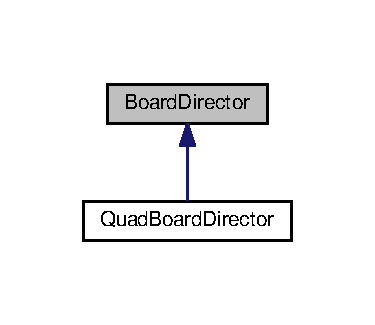
\includegraphics[width=180pt]{classBoardDirector__inherit__graph}
\end{center}
\end{figure}
\subsection*{Public Member Functions}
\begin{DoxyCompactItemize}
\item 
virtual \hyperlink{classBoard}{Board} $\ast$ \hyperlink{classBoardDirector_a4f63215446ecbb9eee811a5f1b848fff}{build} ()=0
\end{DoxyCompactItemize}


\subsection{Member Function Documentation}
\index{Board\+Director@{Board\+Director}!build@{build}}
\index{build@{build}!Board\+Director@{Board\+Director}}
\subsubsection[{\texorpdfstring{build()=0}{build()=0}}]{\setlength{\rightskip}{0pt plus 5cm}virtual {\bf Board}$\ast$ Board\+Director\+::build (
\begin{DoxyParamCaption}
{}
\end{DoxyParamCaption}
)\hspace{0.3cm}{\ttfamily [pure virtual]}}\hypertarget{classBoardDirector_a4f63215446ecbb9eee811a5f1b848fff}{}\label{classBoardDirector_a4f63215446ecbb9eee811a5f1b848fff}


Implemented in \hyperlink{classQuadBoardDirector_a4f43bce7847e996d4a1043c83d81638c}{Quad\+Board\+Director}.



The documentation for this class was generated from the following file\+:\begin{DoxyCompactItemize}
\item 
\hyperlink{BoardBuilder_8hpp}{Board\+Builder.\+hpp}\end{DoxyCompactItemize}

\hypertarget{classByteTranscriber}{}\section{Byte\+Transcriber Class Reference}
\label{classByteTranscriber}\index{Byte\+Transcriber@{Byte\+Transcriber}}


{\ttfamily \#include $<$Byte\+Transcriber.\+hpp$>$}



Inheritance diagram for Byte\+Transcriber\+:\nopagebreak
\begin{figure}[H]
\begin{center}
\leavevmode
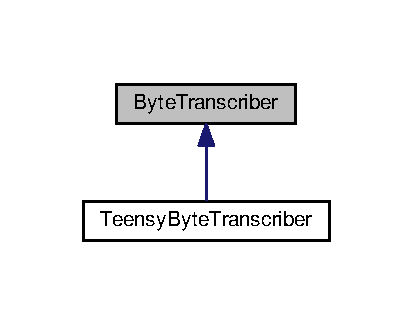
\includegraphics[width=198pt]{classByteTranscriber__inherit__graph}
\end{center}
\end{figure}
\subsection*{Public Member Functions}
\begin{DoxyCompactItemize}
\item 
virtual void \hyperlink{classByteTranscriber_aaa1923f00ab3c7ceb1c3950b58675ff1}{decode\+Joint\+Select} (int $\ast$selects, double encoded\+\_\+double\+\_\+select)=0
\item 
virtual float \hyperlink{classByteTranscriber_a3f987f47dd4d91a30aa601aa783245c7}{encode\+Joint\+Select} (int $\ast$selects)=0
\item 
virtual void \hyperlink{classByteTranscriber_a52bfcc7d5b0bb422392a41172312b681}{decode\+Doubles} (double $\ast$doubles, char $\ast$bytes, int amount)=0
\item 
virtual void \hyperlink{classByteTranscriber_a17c931000510f7595dca00f950ebd6d2}{encode\+Float} (char $\ast$bytes, float $\ast$vals, int amount)=0
\end{DoxyCompactItemize}


\subsection{Member Function Documentation}
\index{Byte\+Transcriber@{Byte\+Transcriber}!decode\+Doubles@{decode\+Doubles}}
\index{decode\+Doubles@{decode\+Doubles}!Byte\+Transcriber@{Byte\+Transcriber}}
\subsubsection[{\texorpdfstring{decode\+Doubles(double $\ast$doubles, char $\ast$bytes, int amount)=0}{decodeDoubles(double *doubles, char *bytes, int amount)=0}}]{\setlength{\rightskip}{0pt plus 5cm}virtual void Byte\+Transcriber\+::decode\+Doubles (
\begin{DoxyParamCaption}
\item[{double $\ast$}]{doubles, }
\item[{char $\ast$}]{bytes, }
\item[{int}]{amount}
\end{DoxyParamCaption}
)\hspace{0.3cm}{\ttfamily [pure virtual]}}\hypertarget{classByteTranscriber_a52bfcc7d5b0bb422392a41172312b681}{}\label{classByteTranscriber_a52bfcc7d5b0bb422392a41172312b681}


Implemented in \hyperlink{classTeensyByteTranscriber_ac62e36acea0f30aca6942322547b34e8}{Teensy\+Byte\+Transcriber}.

\index{Byte\+Transcriber@{Byte\+Transcriber}!decode\+Joint\+Select@{decode\+Joint\+Select}}
\index{decode\+Joint\+Select@{decode\+Joint\+Select}!Byte\+Transcriber@{Byte\+Transcriber}}
\subsubsection[{\texorpdfstring{decode\+Joint\+Select(int $\ast$selects, double encoded\+\_\+double\+\_\+select)=0}{decodeJointSelect(int *selects, double encoded_double_select)=0}}]{\setlength{\rightskip}{0pt plus 5cm}virtual void Byte\+Transcriber\+::decode\+Joint\+Select (
\begin{DoxyParamCaption}
\item[{int $\ast$}]{selects, }
\item[{double}]{encoded\+\_\+double\+\_\+select}
\end{DoxyParamCaption}
)\hspace{0.3cm}{\ttfamily [pure virtual]}}\hypertarget{classByteTranscriber_aaa1923f00ab3c7ceb1c3950b58675ff1}{}\label{classByteTranscriber_aaa1923f00ab3c7ceb1c3950b58675ff1}


Implemented in \hyperlink{classTeensyByteTranscriber_a1a5cfad4100637cdd2d6d971ac0114bb}{Teensy\+Byte\+Transcriber}.

\index{Byte\+Transcriber@{Byte\+Transcriber}!encode\+Float@{encode\+Float}}
\index{encode\+Float@{encode\+Float}!Byte\+Transcriber@{Byte\+Transcriber}}
\subsubsection[{\texorpdfstring{encode\+Float(char $\ast$bytes, float $\ast$vals, int amount)=0}{encodeFloat(char *bytes, float *vals, int amount)=0}}]{\setlength{\rightskip}{0pt plus 5cm}virtual void Byte\+Transcriber\+::encode\+Float (
\begin{DoxyParamCaption}
\item[{char $\ast$}]{bytes, }
\item[{float $\ast$}]{vals, }
\item[{int}]{amount}
\end{DoxyParamCaption}
)\hspace{0.3cm}{\ttfamily [pure virtual]}}\hypertarget{classByteTranscriber_a17c931000510f7595dca00f950ebd6d2}{}\label{classByteTranscriber_a17c931000510f7595dca00f950ebd6d2}


Implemented in \hyperlink{classTeensyByteTranscriber_a87eef9fe6473571a4d8decece1eb6a96}{Teensy\+Byte\+Transcriber}.

\index{Byte\+Transcriber@{Byte\+Transcriber}!encode\+Joint\+Select@{encode\+Joint\+Select}}
\index{encode\+Joint\+Select@{encode\+Joint\+Select}!Byte\+Transcriber@{Byte\+Transcriber}}
\subsubsection[{\texorpdfstring{encode\+Joint\+Select(int $\ast$selects)=0}{encodeJointSelect(int *selects)=0}}]{\setlength{\rightskip}{0pt plus 5cm}virtual float Byte\+Transcriber\+::encode\+Joint\+Select (
\begin{DoxyParamCaption}
\item[{int $\ast$}]{selects}
\end{DoxyParamCaption}
)\hspace{0.3cm}{\ttfamily [pure virtual]}}\hypertarget{classByteTranscriber_a3f987f47dd4d91a30aa601aa783245c7}{}\label{classByteTranscriber_a3f987f47dd4d91a30aa601aa783245c7}


Implemented in \hyperlink{classTeensyByteTranscriber_a7aba78c64f01b2d840f8c96da0f3f97e}{Teensy\+Byte\+Transcriber}.



The documentation for this class was generated from the following file\+:\begin{DoxyCompactItemize}
\item 
\hyperlink{ByteTranscriber_8hpp}{Byte\+Transcriber.\+hpp}\end{DoxyCompactItemize}

\hypertarget{classCalibrateAllFsrsCommand}{}\section{Calibrate\+All\+Fsrs\+Command Class Reference}
\label{classCalibrateAllFsrsCommand}\index{Calibrate\+All\+Fsrs\+Command@{Calibrate\+All\+Fsrs\+Command}}


{\ttfamily \#include $<$Commands.\+hpp$>$}



Inheritance diagram for Calibrate\+All\+Fsrs\+Command\+:\nopagebreak
\begin{figure}[H]
\begin{center}
\leavevmode
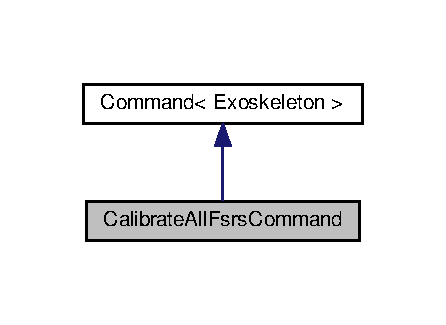
\includegraphics[width=214pt]{classCalibrateAllFsrsCommand__inherit__graph}
\end{center}
\end{figure}


Collaboration diagram for Calibrate\+All\+Fsrs\+Command\+:\nopagebreak
\begin{figure}[H]
\begin{center}
\leavevmode
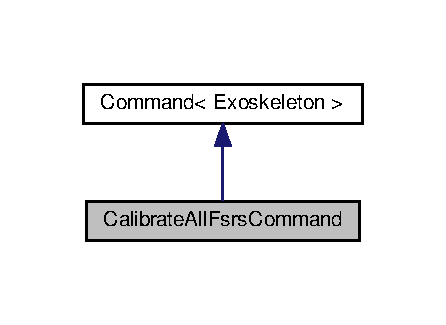
\includegraphics[width=214pt]{classCalibrateAllFsrsCommand__coll__graph}
\end{center}
\end{figure}
\subsection*{Public Member Functions}
\begin{DoxyCompactItemize}
\item 
virtual void \hyperlink{classCalibrateAllFsrsCommand_af0f05f335047e419fb8edb459205f5ae}{execute} (\hyperlink{classExoskeleton}{Exoskeleton} $\ast$exo)
\end{DoxyCompactItemize}


\subsection{Member Function Documentation}
\index{Calibrate\+All\+Fsrs\+Command@{Calibrate\+All\+Fsrs\+Command}!execute@{execute}}
\index{execute@{execute}!Calibrate\+All\+Fsrs\+Command@{Calibrate\+All\+Fsrs\+Command}}
\subsubsection[{\texorpdfstring{execute(\+Exoskeleton $\ast$exo)}{execute(Exoskeleton *exo)}}]{\setlength{\rightskip}{0pt plus 5cm}void Calibrate\+All\+Fsrs\+Command\+::execute (
\begin{DoxyParamCaption}
\item[{{\bf Exoskeleton} $\ast$}]{exo}
\end{DoxyParamCaption}
)\hspace{0.3cm}{\ttfamily [virtual]}}\hypertarget{classCalibrateAllFsrsCommand_af0f05f335047e419fb8edb459205f5ae}{}\label{classCalibrateAllFsrsCommand_af0f05f335047e419fb8edb459205f5ae}


Implements \hyperlink{classCommand_af8fc41633b1d53b23da6a99c81c0689c}{Command$<$ Exoskeleton $>$}.



The documentation for this class was generated from the following files\+:\begin{DoxyCompactItemize}
\item 
\hyperlink{Commands_8hpp}{Commands.\+hpp}\item 
\hyperlink{Commands_8cpp}{Commands.\+cpp}\end{DoxyCompactItemize}

\hypertarget{classCalibrateAllTorquesCommand}{}\section{Calibrate\+All\+Torques\+Command Class Reference}
\label{classCalibrateAllTorquesCommand}\index{Calibrate\+All\+Torques\+Command@{Calibrate\+All\+Torques\+Command}}


{\ttfamily \#include $<$Commands.\+hpp$>$}



Inheritance diagram for Calibrate\+All\+Torques\+Command\+:\nopagebreak
\begin{figure}[H]
\begin{center}
\leavevmode
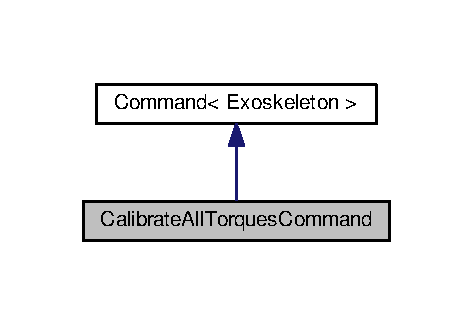
\includegraphics[width=227pt]{classCalibrateAllTorquesCommand__inherit__graph}
\end{center}
\end{figure}


Collaboration diagram for Calibrate\+All\+Torques\+Command\+:\nopagebreak
\begin{figure}[H]
\begin{center}
\leavevmode
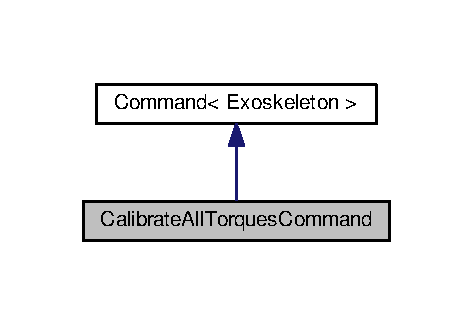
\includegraphics[width=227pt]{classCalibrateAllTorquesCommand__coll__graph}
\end{center}
\end{figure}
\subsection*{Public Member Functions}
\begin{DoxyCompactItemize}
\item 
virtual void \hyperlink{classCalibrateAllTorquesCommand_a5c63662eccb63e656139bcac460e5eb8}{execute} (\hyperlink{classExoskeleton}{Exoskeleton} $\ast$exo)
\end{DoxyCompactItemize}


\subsection{Member Function Documentation}
\index{Calibrate\+All\+Torques\+Command@{Calibrate\+All\+Torques\+Command}!execute@{execute}}
\index{execute@{execute}!Calibrate\+All\+Torques\+Command@{Calibrate\+All\+Torques\+Command}}
\subsubsection[{\texorpdfstring{execute(\+Exoskeleton $\ast$exo)}{execute(Exoskeleton *exo)}}]{\setlength{\rightskip}{0pt plus 5cm}void Calibrate\+All\+Torques\+Command\+::execute (
\begin{DoxyParamCaption}
\item[{{\bf Exoskeleton} $\ast$}]{exo}
\end{DoxyParamCaption}
)\hspace{0.3cm}{\ttfamily [virtual]}}\hypertarget{classCalibrateAllTorquesCommand_a5c63662eccb63e656139bcac460e5eb8}{}\label{classCalibrateAllTorquesCommand_a5c63662eccb63e656139bcac460e5eb8}


Implements \hyperlink{classCommand_af8fc41633b1d53b23da6a99c81c0689c}{Command$<$ Exoskeleton $>$}.



The documentation for this class was generated from the following files\+:\begin{DoxyCompactItemize}
\item 
\hyperlink{Commands_8hpp}{Commands.\+hpp}\item 
\hyperlink{Commands_8cpp}{Commands.\+cpp}\end{DoxyCompactItemize}

\hypertarget{classCalibrateFsrTransmission}{}\section{Calibrate\+Fsr\+Transmission Class Reference}
\label{classCalibrateFsrTransmission}\index{Calibrate\+Fsr\+Transmission@{Calibrate\+Fsr\+Transmission}}


{\ttfamily \#include $<$Transmission.\+hpp$>$}



Inheritance diagram for Calibrate\+Fsr\+Transmission\+:\nopagebreak
\begin{figure}[H]
\begin{center}
\leavevmode
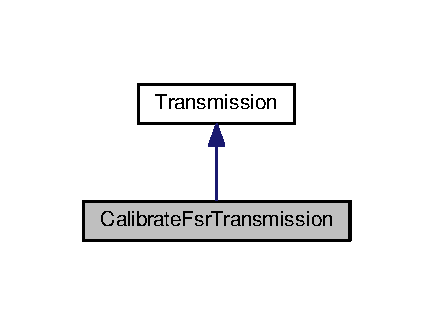
\includegraphics[width=208pt]{classCalibrateFsrTransmission__inherit__graph}
\end{center}
\end{figure}


Collaboration diagram for Calibrate\+Fsr\+Transmission\+:\nopagebreak
\begin{figure}[H]
\begin{center}
\leavevmode
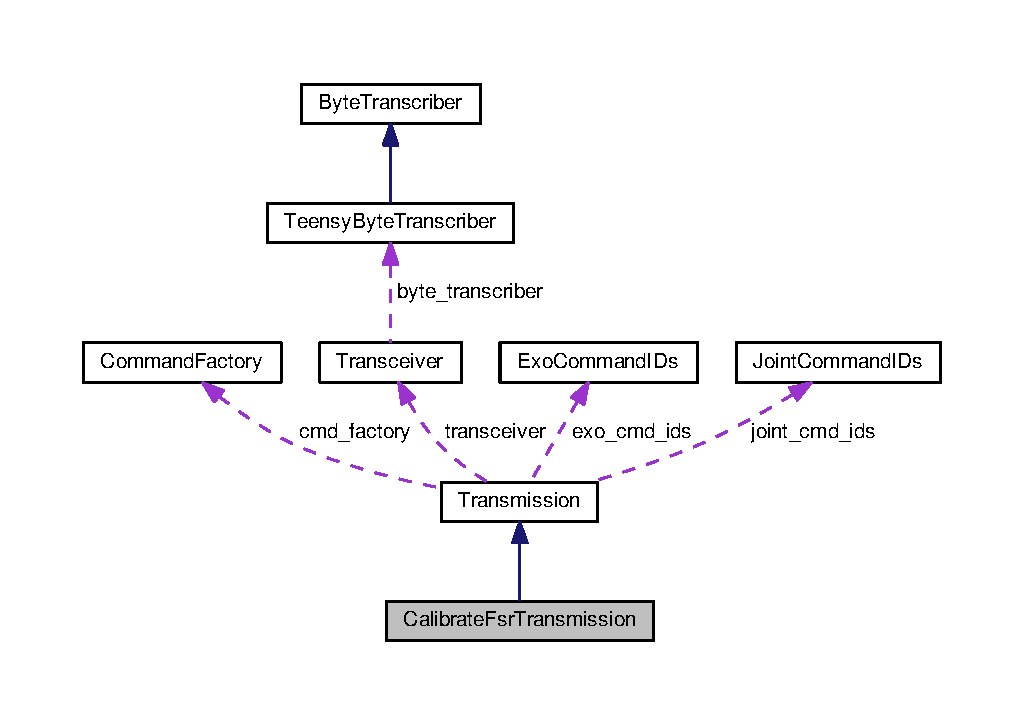
\includegraphics[width=350pt]{classCalibrateFsrTransmission__coll__graph}
\end{center}
\end{figure}
\subsection*{Public Member Functions}
\begin{DoxyCompactItemize}
\item 
\hyperlink{classCalibrateFsrTransmission_a837e7638649ab9692aa84dcad6515113}{Calibrate\+Fsr\+Transmission} (\hyperlink{classTransceiver}{Transceiver} $\ast$\hyperlink{classTransmission_a4136f9d979a928565232a2d3d6eb5ac5}{transceiver}, \hyperlink{classCommandFactory}{Command\+Factory} $\ast$cmd)
\end{DoxyCompactItemize}
\subsection*{Additional Inherited Members}


\subsection{Constructor \& Destructor Documentation}
\index{Calibrate\+Fsr\+Transmission@{Calibrate\+Fsr\+Transmission}!Calibrate\+Fsr\+Transmission@{Calibrate\+Fsr\+Transmission}}
\index{Calibrate\+Fsr\+Transmission@{Calibrate\+Fsr\+Transmission}!Calibrate\+Fsr\+Transmission@{Calibrate\+Fsr\+Transmission}}
\subsubsection[{\texorpdfstring{Calibrate\+Fsr\+Transmission(\+Transceiver $\ast$transceiver, Command\+Factory $\ast$cmd)}{CalibrateFsrTransmission(Transceiver *transceiver, CommandFactory *cmd)}}]{\setlength{\rightskip}{0pt plus 5cm}Calibrate\+Fsr\+Transmission\+::\+Calibrate\+Fsr\+Transmission (
\begin{DoxyParamCaption}
\item[{{\bf Transceiver} $\ast$}]{transceiver, }
\item[{{\bf Command\+Factory} $\ast$}]{cmd}
\end{DoxyParamCaption}
)\hspace{0.3cm}{\ttfamily [explicit]}}\hypertarget{classCalibrateFsrTransmission_a837e7638649ab9692aa84dcad6515113}{}\label{classCalibrateFsrTransmission_a837e7638649ab9692aa84dcad6515113}


The documentation for this class was generated from the following files\+:\begin{DoxyCompactItemize}
\item 
\hyperlink{Transmission_8hpp}{Transmission.\+hpp}\item 
\hyperlink{Transmission_8cpp}{Transmission.\+cpp}\end{DoxyCompactItemize}

\hypertarget{classCalibrateTorqueTransmission}{}\section{Calibrate\+Torque\+Transmission Class Reference}
\label{classCalibrateTorqueTransmission}\index{Calibrate\+Torque\+Transmission@{Calibrate\+Torque\+Transmission}}


{\ttfamily \#include $<$Transmission.\+hpp$>$}



Inheritance diagram for Calibrate\+Torque\+Transmission\+:\nopagebreak
\begin{figure}[H]
\begin{center}
\leavevmode
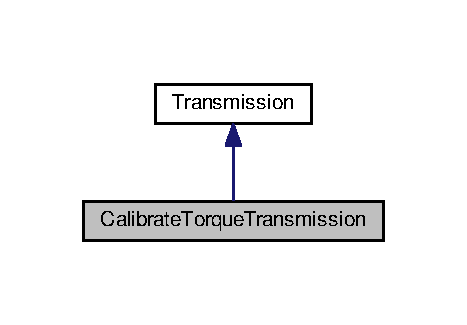
\includegraphics[width=224pt]{classCalibrateTorqueTransmission__inherit__graph}
\end{center}
\end{figure}


Collaboration diagram for Calibrate\+Torque\+Transmission\+:\nopagebreak
\begin{figure}[H]
\begin{center}
\leavevmode
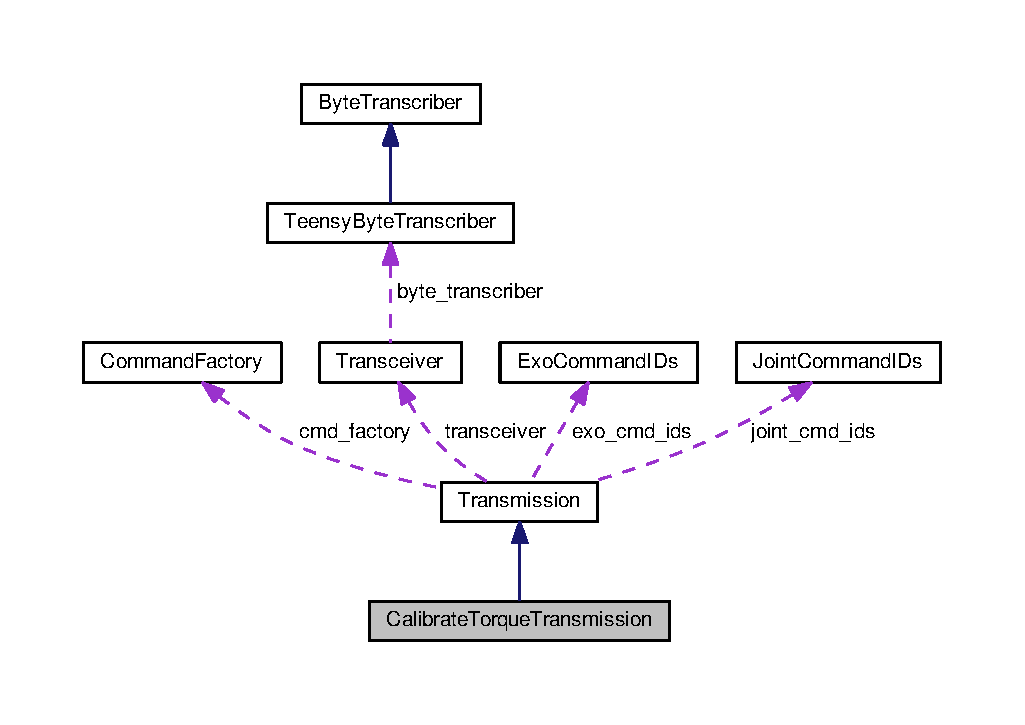
\includegraphics[width=350pt]{classCalibrateTorqueTransmission__coll__graph}
\end{center}
\end{figure}
\subsection*{Public Member Functions}
\begin{DoxyCompactItemize}
\item 
\hyperlink{classCalibrateTorqueTransmission_afe8c79294c58f11898de7ba5408eb238}{Calibrate\+Torque\+Transmission} (\hyperlink{classTransceiver}{Transceiver} $\ast$\hyperlink{classTransmission_a4136f9d979a928565232a2d3d6eb5ac5}{transceiver}, \hyperlink{classCommandFactory}{Command\+Factory} $\ast$cmd)
\end{DoxyCompactItemize}
\subsection*{Additional Inherited Members}


\subsection{Constructor \& Destructor Documentation}
\index{Calibrate\+Torque\+Transmission@{Calibrate\+Torque\+Transmission}!Calibrate\+Torque\+Transmission@{Calibrate\+Torque\+Transmission}}
\index{Calibrate\+Torque\+Transmission@{Calibrate\+Torque\+Transmission}!Calibrate\+Torque\+Transmission@{Calibrate\+Torque\+Transmission}}
\subsubsection[{\texorpdfstring{Calibrate\+Torque\+Transmission(\+Transceiver $\ast$transceiver, Command\+Factory $\ast$cmd)}{CalibrateTorqueTransmission(Transceiver *transceiver, CommandFactory *cmd)}}]{\setlength{\rightskip}{0pt plus 5cm}Calibrate\+Torque\+Transmission\+::\+Calibrate\+Torque\+Transmission (
\begin{DoxyParamCaption}
\item[{{\bf Transceiver} $\ast$}]{transceiver, }
\item[{{\bf Command\+Factory} $\ast$}]{cmd}
\end{DoxyParamCaption}
)\hspace{0.3cm}{\ttfamily [explicit]}}\hypertarget{classCalibrateTorqueTransmission_afe8c79294c58f11898de7ba5408eb238}{}\label{classCalibrateTorqueTransmission_afe8c79294c58f11898de7ba5408eb238}


The documentation for this class was generated from the following files\+:\begin{DoxyCompactItemize}
\item 
\hyperlink{Transmission_8hpp}{Transmission.\+hpp}\item 
\hyperlink{Transmission_8cpp}{Transmission.\+cpp}\end{DoxyCompactItemize}

\hypertarget{classChangeTrigger}{}\section{Change\+Trigger Class Reference}
\label{classChangeTrigger}\index{Change\+Trigger@{Change\+Trigger}}


{\ttfamily \#include $<$Utils.\+hpp$>$}

\subsection*{Public Member Functions}
\begin{DoxyCompactItemize}
\item 
\hyperlink{classChangeTrigger_a9653aa6762683dd2d6ad364cb37e170b}{Change\+Trigger} (bool start\+\_\+state)
\item 
bool \hyperlink{classChangeTrigger_aab87643df431ed54be4b938234e5a965}{update} (bool state)
\end{DoxyCompactItemize}


\subsection{Constructor \& Destructor Documentation}
\index{Change\+Trigger@{Change\+Trigger}!Change\+Trigger@{Change\+Trigger}}
\index{Change\+Trigger@{Change\+Trigger}!Change\+Trigger@{Change\+Trigger}}
\subsubsection[{\texorpdfstring{Change\+Trigger(bool start\+\_\+state)}{ChangeTrigger(bool start_state)}}]{\setlength{\rightskip}{0pt plus 5cm}Change\+Trigger\+::\+Change\+Trigger (
\begin{DoxyParamCaption}
\item[{bool}]{start\+\_\+state}
\end{DoxyParamCaption}
)}\hypertarget{classChangeTrigger_a9653aa6762683dd2d6ad364cb37e170b}{}\label{classChangeTrigger_a9653aa6762683dd2d6ad364cb37e170b}


\subsection{Member Function Documentation}
\index{Change\+Trigger@{Change\+Trigger}!update@{update}}
\index{update@{update}!Change\+Trigger@{Change\+Trigger}}
\subsubsection[{\texorpdfstring{update(bool state)}{update(bool state)}}]{\setlength{\rightskip}{0pt plus 5cm}bool Change\+Trigger\+::update (
\begin{DoxyParamCaption}
\item[{bool}]{state}
\end{DoxyParamCaption}
)}\hypertarget{classChangeTrigger_aab87643df431ed54be4b938234e5a965}{}\label{classChangeTrigger_aab87643df431ed54be4b938234e5a965}


The documentation for this class was generated from the following files\+:\begin{DoxyCompactItemize}
\item 
\hyperlink{Utils_8hpp}{Utils.\+hpp}\item 
\hyperlink{Utils_8cpp}{Utils.\+cpp}\end{DoxyCompactItemize}

\hypertarget{classCheckBluetoothTransmission}{}\section{Check\+Bluetooth\+Transmission Class Reference}
\label{classCheckBluetoothTransmission}\index{Check\+Bluetooth\+Transmission@{Check\+Bluetooth\+Transmission}}


{\ttfamily \#include $<$Transmission.\+hpp$>$}



Inheritance diagram for Check\+Bluetooth\+Transmission\+:\nopagebreak
\begin{figure}[H]
\begin{center}
\leavevmode
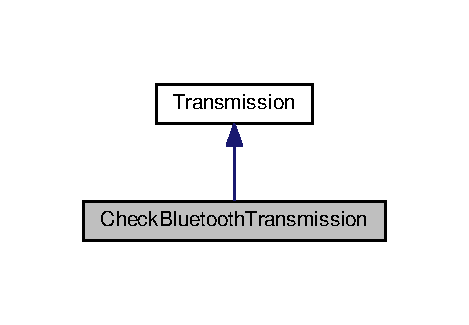
\includegraphics[width=225pt]{classCheckBluetoothTransmission__inherit__graph}
\end{center}
\end{figure}


Collaboration diagram for Check\+Bluetooth\+Transmission\+:\nopagebreak
\begin{figure}[H]
\begin{center}
\leavevmode
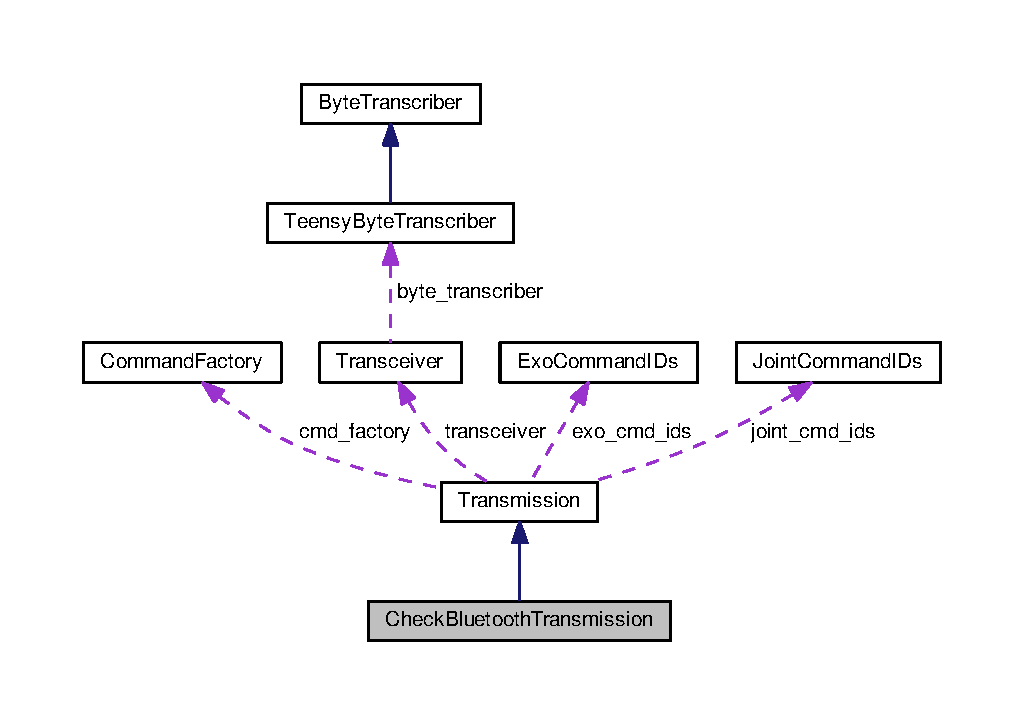
\includegraphics[width=350pt]{classCheckBluetoothTransmission__coll__graph}
\end{center}
\end{figure}
\subsection*{Public Member Functions}
\begin{DoxyCompactItemize}
\item 
\hyperlink{classCheckBluetoothTransmission_ad1e2e1588b7e33d0b06d80bb06beab7f}{Check\+Bluetooth\+Transmission} (\hyperlink{classTransceiver}{Transceiver} $\ast$\hyperlink{classTransmission_a4136f9d979a928565232a2d3d6eb5ac5}{transceiver}, \hyperlink{classCommandFactory}{Command\+Factory} $\ast$cmd)
\end{DoxyCompactItemize}
\subsection*{Additional Inherited Members}


\subsection{Constructor \& Destructor Documentation}
\index{Check\+Bluetooth\+Transmission@{Check\+Bluetooth\+Transmission}!Check\+Bluetooth\+Transmission@{Check\+Bluetooth\+Transmission}}
\index{Check\+Bluetooth\+Transmission@{Check\+Bluetooth\+Transmission}!Check\+Bluetooth\+Transmission@{Check\+Bluetooth\+Transmission}}
\subsubsection[{\texorpdfstring{Check\+Bluetooth\+Transmission(\+Transceiver $\ast$transceiver, Command\+Factory $\ast$cmd)}{CheckBluetoothTransmission(Transceiver *transceiver, CommandFactory *cmd)}}]{\setlength{\rightskip}{0pt plus 5cm}Check\+Bluetooth\+Transmission\+::\+Check\+Bluetooth\+Transmission (
\begin{DoxyParamCaption}
\item[{{\bf Transceiver} $\ast$}]{transceiver, }
\item[{{\bf Command\+Factory} $\ast$}]{cmd}
\end{DoxyParamCaption}
)\hspace{0.3cm}{\ttfamily [explicit]}}\hypertarget{classCheckBluetoothTransmission_ad1e2e1588b7e33d0b06d80bb06beab7f}{}\label{classCheckBluetoothTransmission_ad1e2e1588b7e33d0b06d80bb06beab7f}


The documentation for this class was generated from the following files\+:\begin{DoxyCompactItemize}
\item 
\hyperlink{Transmission_8hpp}{Transmission.\+hpp}\item 
\hyperlink{Transmission_8cpp}{Transmission.\+cpp}\end{DoxyCompactItemize}

\hypertarget{classCheckMemoryTransmission}{}\section{Check\+Memory\+Transmission Class Reference}
\label{classCheckMemoryTransmission}\index{Check\+Memory\+Transmission@{Check\+Memory\+Transmission}}


{\ttfamily \#include $<$Transmission.\+hpp$>$}



Inheritance diagram for Check\+Memory\+Transmission\+:\nopagebreak
\begin{figure}[H]
\begin{center}
\leavevmode
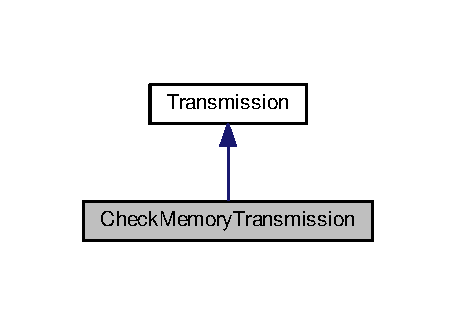
\includegraphics[width=219pt]{classCheckMemoryTransmission__inherit__graph}
\end{center}
\end{figure}


Collaboration diagram for Check\+Memory\+Transmission\+:\nopagebreak
\begin{figure}[H]
\begin{center}
\leavevmode
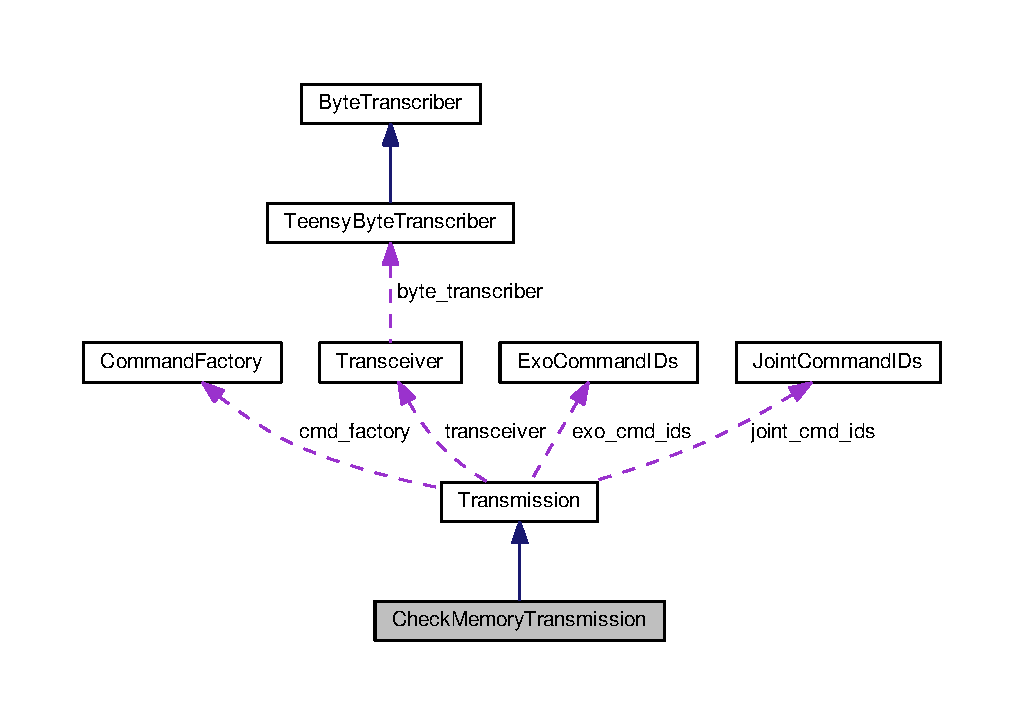
\includegraphics[width=350pt]{classCheckMemoryTransmission__coll__graph}
\end{center}
\end{figure}
\subsection*{Public Member Functions}
\begin{DoxyCompactItemize}
\item 
\hyperlink{classCheckMemoryTransmission_abcfde5b7d393f59281c2cd6b3e9c34e6}{Check\+Memory\+Transmission} (\hyperlink{classTransceiver}{Transceiver} $\ast$\hyperlink{classTransmission_a4136f9d979a928565232a2d3d6eb5ac5}{transceiver}, \hyperlink{classCommandFactory}{Command\+Factory} $\ast$cmd)
\end{DoxyCompactItemize}
\subsection*{Additional Inherited Members}


\subsection{Constructor \& Destructor Documentation}
\index{Check\+Memory\+Transmission@{Check\+Memory\+Transmission}!Check\+Memory\+Transmission@{Check\+Memory\+Transmission}}
\index{Check\+Memory\+Transmission@{Check\+Memory\+Transmission}!Check\+Memory\+Transmission@{Check\+Memory\+Transmission}}
\subsubsection[{\texorpdfstring{Check\+Memory\+Transmission(\+Transceiver $\ast$transceiver, Command\+Factory $\ast$cmd)}{CheckMemoryTransmission(Transceiver *transceiver, CommandFactory *cmd)}}]{\setlength{\rightskip}{0pt plus 5cm}Check\+Memory\+Transmission\+::\+Check\+Memory\+Transmission (
\begin{DoxyParamCaption}
\item[{{\bf Transceiver} $\ast$}]{transceiver, }
\item[{{\bf Command\+Factory} $\ast$}]{cmd}
\end{DoxyParamCaption}
)\hspace{0.3cm}{\ttfamily [explicit]}}\hypertarget{classCheckMemoryTransmission_abcfde5b7d393f59281c2cd6b3e9c34e6}{}\label{classCheckMemoryTransmission_abcfde5b7d393f59281c2cd6b3e9c34e6}


The documentation for this class was generated from the following files\+:\begin{DoxyCompactItemize}
\item 
\hyperlink{Transmission_8hpp}{Transmission.\+hpp}\item 
\hyperlink{Transmission_8cpp}{Transmission.\+cpp}\end{DoxyCompactItemize}

\hypertarget{classChrono}{}\section{Chrono Class Reference}
\label{classChrono}\index{Chrono@{Chrono}}


{\ttfamily \#include $<$Utils.\+hpp$>$}

\subsection*{Public Member Functions}
\begin{DoxyCompactItemize}
\item 
\hyperlink{classChrono_af6434dc40b83176354778928c6e2893e}{Chrono} (unsigned long interval)
\item 
bool \hyperlink{classChrono_a74c5c1ece9bda298177efe627486ded7}{check} ()
\item 
void \hyperlink{classChrono_a027be23720616639bc610a98c53740ea}{reset} ()
\end{DoxyCompactItemize}


\subsection{Constructor \& Destructor Documentation}
\index{Chrono@{Chrono}!Chrono@{Chrono}}
\index{Chrono@{Chrono}!Chrono@{Chrono}}
\subsubsection[{\texorpdfstring{Chrono(unsigned long interval)}{Chrono(unsigned long interval)}}]{\setlength{\rightskip}{0pt plus 5cm}Chrono\+::\+Chrono (
\begin{DoxyParamCaption}
\item[{unsigned long}]{interval}
\end{DoxyParamCaption}
)}\hypertarget{classChrono_af6434dc40b83176354778928c6e2893e}{}\label{classChrono_af6434dc40b83176354778928c6e2893e}


\subsection{Member Function Documentation}
\index{Chrono@{Chrono}!check@{check}}
\index{check@{check}!Chrono@{Chrono}}
\subsubsection[{\texorpdfstring{check()}{check()}}]{\setlength{\rightskip}{0pt plus 5cm}bool Chrono\+::check (
\begin{DoxyParamCaption}
{}
\end{DoxyParamCaption}
)}\hypertarget{classChrono_a74c5c1ece9bda298177efe627486ded7}{}\label{classChrono_a74c5c1ece9bda298177efe627486ded7}
\index{Chrono@{Chrono}!reset@{reset}}
\index{reset@{reset}!Chrono@{Chrono}}
\subsubsection[{\texorpdfstring{reset()}{reset()}}]{\setlength{\rightskip}{0pt plus 5cm}void Chrono\+::reset (
\begin{DoxyParamCaption}
{}
\end{DoxyParamCaption}
)}\hypertarget{classChrono_a027be23720616639bc610a98c53740ea}{}\label{classChrono_a027be23720616639bc610a98c53740ea}


The documentation for this class was generated from the following files\+:\begin{DoxyCompactItemize}
\item 
\hyperlink{Utils_8hpp}{Utils.\+hpp}\item 
\hyperlink{Utils_8cpp}{Utils.\+cpp}\end{DoxyCompactItemize}

\hypertarget{classClamp}{}\section{Clamp Class Reference}
\label{classClamp}\index{Clamp@{Clamp}}


A class to clamp values.  




{\ttfamily \#include $<$Utils.\+hpp$>$}

\subsection*{Public Member Functions}
\begin{DoxyCompactItemize}
\item 
\hyperlink{classClamp_a728a84cf8827958105210cf776e6497e}{Clamp} (double lower, double upper)
\begin{DoxyCompactList}\small\item\em The constructor with upper and lower bounds. \end{DoxyCompactList}\item 
double \hyperlink{classClamp_a0d371f34a552d9fcd9982b8d38ff9e19}{clamp} (double value)
\begin{DoxyCompactList}\small\item\em Clamps the value between lower and upper. \end{DoxyCompactList}\end{DoxyCompactItemize}


\subsection{Detailed Description}
A class to clamp values. 

The clamp class will always clamp the given value between the upper and lower values given. 

\subsection{Constructor \& Destructor Documentation}
\index{Clamp@{Clamp}!Clamp@{Clamp}}
\index{Clamp@{Clamp}!Clamp@{Clamp}}
\subsubsection[{\texorpdfstring{Clamp(double lower, double upper)}{Clamp(double lower, double upper)}}]{\setlength{\rightskip}{0pt plus 5cm}Clamp\+::\+Clamp (
\begin{DoxyParamCaption}
\item[{double}]{lower, }
\item[{double}]{upper}
\end{DoxyParamCaption}
)}\hypertarget{classClamp_a728a84cf8827958105210cf776e6497e}{}\label{classClamp_a728a84cf8827958105210cf776e6497e}


The constructor with upper and lower bounds. 


\begin{DoxyParams}{Parameters}
{\em lower} & The lower bound that the value can\textquotesingle{}t be lower than \\
\hline
{\em upper} & The upper bound that the value can\textquotesingle{}t be higher than\\
\hline
\end{DoxyParams}
The constructor that takes in the upper and lower bounds that the value will be constrained within. 

\subsection{Member Function Documentation}
\index{Clamp@{Clamp}!clamp@{clamp}}
\index{clamp@{clamp}!Clamp@{Clamp}}
\subsubsection[{\texorpdfstring{clamp(double value)}{clamp(double value)}}]{\setlength{\rightskip}{0pt plus 5cm}double Clamp\+::clamp (
\begin{DoxyParamCaption}
\item[{double}]{val}
\end{DoxyParamCaption}
)}\hypertarget{classClamp_a0d371f34a552d9fcd9982b8d38ff9e19}{}\label{classClamp_a0d371f34a552d9fcd9982b8d38ff9e19}


Clamps the value between lower and upper. 


\begin{DoxyParams}{Parameters}
{\em value} & The value to be clamped \\
\hline
\end{DoxyParams}
\begin{DoxyReturn}{Returns}
The clamped value
\end{DoxyReturn}
Constrains the value between the lower and upper value. If value is below lower, it will return lower. If greater than upper returns upper. Else it will return the value given. 

The documentation for this class was generated from the following files\+:\begin{DoxyCompactItemize}
\item 
\hyperlink{Utils_8hpp}{Utils.\+hpp}\item 
\hyperlink{Utils_8cpp}{Utils.\+cpp}\end{DoxyCompactItemize}

\hypertarget{classCleanBluetoothBufferTransmission}{}\section{Clean\+Bluetooth\+Buffer\+Transmission Class Reference}
\label{classCleanBluetoothBufferTransmission}\index{Clean\+Bluetooth\+Buffer\+Transmission@{Clean\+Bluetooth\+Buffer\+Transmission}}


{\ttfamily \#include $<$Transmission.\+hpp$>$}



Inheritance diagram for Clean\+Bluetooth\+Buffer\+Transmission\+:\nopagebreak
\begin{figure}[H]
\begin{center}
\leavevmode
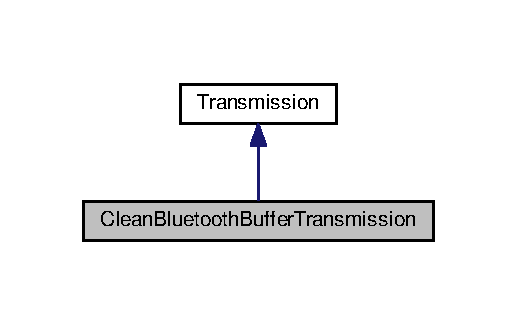
\includegraphics[width=248pt]{classCleanBluetoothBufferTransmission__inherit__graph}
\end{center}
\end{figure}


Collaboration diagram for Clean\+Bluetooth\+Buffer\+Transmission\+:\nopagebreak
\begin{figure}[H]
\begin{center}
\leavevmode
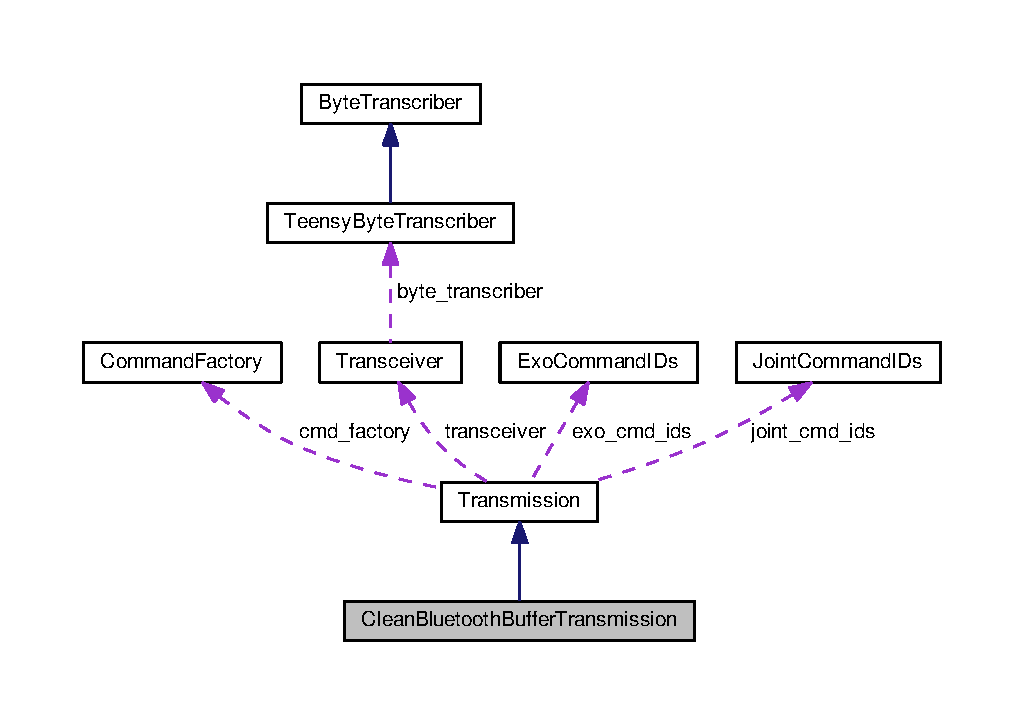
\includegraphics[width=350pt]{classCleanBluetoothBufferTransmission__coll__graph}
\end{center}
\end{figure}
\subsection*{Public Member Functions}
\begin{DoxyCompactItemize}
\item 
\hyperlink{classCleanBluetoothBufferTransmission_a768437c9407e205c302453be325aaa36}{Clean\+Bluetooth\+Buffer\+Transmission} (\hyperlink{classTransceiver}{Transceiver} $\ast$\hyperlink{classTransmission_a4136f9d979a928565232a2d3d6eb5ac5}{transceiver}, \hyperlink{classCommandFactory}{Command\+Factory} $\ast$cmd)
\end{DoxyCompactItemize}
\subsection*{Additional Inherited Members}


\subsection{Constructor \& Destructor Documentation}
\index{Clean\+Bluetooth\+Buffer\+Transmission@{Clean\+Bluetooth\+Buffer\+Transmission}!Clean\+Bluetooth\+Buffer\+Transmission@{Clean\+Bluetooth\+Buffer\+Transmission}}
\index{Clean\+Bluetooth\+Buffer\+Transmission@{Clean\+Bluetooth\+Buffer\+Transmission}!Clean\+Bluetooth\+Buffer\+Transmission@{Clean\+Bluetooth\+Buffer\+Transmission}}
\subsubsection[{\texorpdfstring{Clean\+Bluetooth\+Buffer\+Transmission(\+Transceiver $\ast$transceiver, Command\+Factory $\ast$cmd)}{CleanBluetoothBufferTransmission(Transceiver *transceiver, CommandFactory *cmd)}}]{\setlength{\rightskip}{0pt plus 5cm}Clean\+Bluetooth\+Buffer\+Transmission\+::\+Clean\+Bluetooth\+Buffer\+Transmission (
\begin{DoxyParamCaption}
\item[{{\bf Transceiver} $\ast$}]{transceiver, }
\item[{{\bf Command\+Factory} $\ast$}]{cmd}
\end{DoxyParamCaption}
)\hspace{0.3cm}{\ttfamily [explicit]}}\hypertarget{classCleanBluetoothBufferTransmission_a768437c9407e205c302453be325aaa36}{}\label{classCleanBluetoothBufferTransmission_a768437c9407e205c302453be325aaa36}


The documentation for this class was generated from the following files\+:\begin{DoxyCompactItemize}
\item 
\hyperlink{Transmission_8hpp}{Transmission.\+hpp}\item 
\hyperlink{Transmission_8cpp}{Transmission.\+cpp}\end{DoxyCompactItemize}

\hypertarget{classCommand}{}\section{Command$<$ T $>$ Class Template Reference}
\label{classCommand}\index{Command$<$ T $>$@{Command$<$ T $>$}}


{\ttfamily \#include $<$Commands.\+hpp$>$}

\subsection*{Public Member Functions}
\begin{DoxyCompactItemize}
\item 
virtual \hyperlink{classCommand_aebb12ac3a438274c4739ad09f650b316}{$\sim$\+Command} ()
\item 
virtual void \hyperlink{classCommand_af8fc41633b1d53b23da6a99c81c0689c}{execute} (T $\ast$context)=0
\end{DoxyCompactItemize}


\subsection{Constructor \& Destructor Documentation}
\index{Command@{Command}!````~Command@{$\sim$\+Command}}
\index{````~Command@{$\sim$\+Command}!Command@{Command}}
\subsubsection[{\texorpdfstring{$\sim$\+Command()}{~Command()}}]{\setlength{\rightskip}{0pt plus 5cm}template$<$class T $>$ {\bf Command}$<$ T $>$\+::$\sim${\bf Command} (
\begin{DoxyParamCaption}
{}
\end{DoxyParamCaption}
)\hspace{0.3cm}{\ttfamily [virtual]}}\hypertarget{classCommand_aebb12ac3a438274c4739ad09f650b316}{}\label{classCommand_aebb12ac3a438274c4739ad09f650b316}


\subsection{Member Function Documentation}
\index{Command@{Command}!execute@{execute}}
\index{execute@{execute}!Command@{Command}}
\subsubsection[{\texorpdfstring{execute(\+T $\ast$context)=0}{execute(T *context)=0}}]{\setlength{\rightskip}{0pt plus 5cm}template$<$class T$>$ virtual void {\bf Command}$<$ T $>$\+::execute (
\begin{DoxyParamCaption}
\item[{T $\ast$}]{context}
\end{DoxyParamCaption}
)\hspace{0.3cm}{\ttfamily [pure virtual]}}\hypertarget{classCommand_af8fc41633b1d53b23da6a99c81c0689c}{}\label{classCommand_af8fc41633b1d53b23da6a99c81c0689c}


Implemented in \hyperlink{classSetJointSmoothingParamCommand_a1ea658af81e810b3f5344816705a3c56}{Set\+Joint\+Smoothing\+Param\+Command}, \hyperlink{classSetJointKfCommand_a9b4b5e47aec44dd405273526a254b8cb}{Set\+Joint\+Kf\+Command}, \hyperlink{classSetJointPidCommand_aa7a930ba0a725cc63117682703a58bad}{Set\+Joint\+Pid\+Command}, \hyperlink{classSetJointSetpointCommand_a7f1341d238595b02a660fb55aef9bc45}{Set\+Joint\+Setpoint\+Command}, \hyperlink{classCalibrateAllFsrsCommand_af0f05f335047e419fb8edb459205f5ae}{Calibrate\+All\+Fsrs\+Command}, \hyperlink{classCalibrateAllTorquesCommand_a5c63662eccb63e656139bcac460e5eb8}{Calibrate\+All\+Torques\+Command}, \hyperlink{classEndTrialCommand_ac07f0eddff9b21da6cb302489aac19c7}{End\+Trial\+Command}, and \hyperlink{classStartTrialCommand_a3b3772ca308e89554da05751a3255e4f}{Start\+Trial\+Command}.



The documentation for this class was generated from the following files\+:\begin{DoxyCompactItemize}
\item 
\hyperlink{Commands_8hpp}{Commands.\+hpp}\item 
\hyperlink{Commands_8cpp}{Commands.\+cpp}\end{DoxyCompactItemize}

\hypertarget{classCommandFactory}{}\section{Command\+Factory Class Reference}
\label{classCommandFactory}\index{Command\+Factory@{Command\+Factory}}


{\ttfamily \#include $<$Commands.\+hpp$>$}



Inheritance diagram for Command\+Factory\+:\nopagebreak
\begin{figure}[H]
\begin{center}
\leavevmode
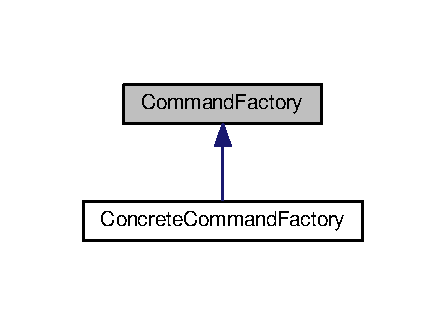
\includegraphics[width=214pt]{classCommandFactory__inherit__graph}
\end{center}
\end{figure}
\subsection*{Public Member Functions}
\begin{DoxyCompactItemize}
\item 
\hyperlink{classCommandFactory_aca190eaa40840830df307dec5f7f36ef}{Command\+Factory} ()
\item 
virtual \hyperlink{classCommandFactory_a7bb4a37a7903caf0e42207b7ec8a6ad6}{$\sim$\+Command\+Factory} ()
\item 
virtual \hyperlink{classCommand}{Command}$<$ \hyperlink{classJoint}{Joint} $>$ $\ast$ \hyperlink{classCommandFactory_acdc303aaceaf41b5f53d92e7379d851e}{create\+Joint\+Command} (\hyperlink{Commands_8hpp_a350356b969551ce1a95947b3cec75d56}{Joint\+Command\+ID} id, \hyperlink{States_8hpp_a26aafbeccd8f356b39e1809f1ab9cfdc}{State\+ID} state, double value)=0
\item 
virtual \hyperlink{classCommand}{Command}$<$ \hyperlink{classJoint}{Joint} $>$ $\ast$ \hyperlink{classCommandFactory_af1813c30ede407362ea395c978f24963}{create\+Joint\+Command} (\hyperlink{Commands_8hpp_a350356b969551ce1a95947b3cec75d56}{Joint\+Command\+ID} id, double, double, double)=0
\item 
virtual \hyperlink{classCommand}{Command}$<$ \hyperlink{classJoint}{Joint} $>$ $\ast$ \hyperlink{classCommandFactory_accade06a34e2d9424ec9765543617e39}{create\+Joint\+Command} (\hyperlink{Commands_8hpp_a350356b969551ce1a95947b3cec75d56}{Joint\+Command\+ID} id, double)=0
\item 
virtual \hyperlink{classCommand}{Command}$<$ \hyperlink{classExoskeleton}{Exoskeleton} $>$ $\ast$ \hyperlink{classCommandFactory_a9cd75aee1d86b52a0c5da5abada1855e}{create\+Exo\+Command} (\hyperlink{Commands_8hpp_a4a0419b573bf683fef9162331e6ec74e}{Exo\+Command\+ID})=0
\end{DoxyCompactItemize}


\subsection{Constructor \& Destructor Documentation}
\index{Command\+Factory@{Command\+Factory}!Command\+Factory@{Command\+Factory}}
\index{Command\+Factory@{Command\+Factory}!Command\+Factory@{Command\+Factory}}
\subsubsection[{\texorpdfstring{Command\+Factory()}{CommandFactory()}}]{\setlength{\rightskip}{0pt plus 5cm}Command\+Factory\+::\+Command\+Factory (
\begin{DoxyParamCaption}
{}
\end{DoxyParamCaption}
)}\hypertarget{classCommandFactory_aca190eaa40840830df307dec5f7f36ef}{}\label{classCommandFactory_aca190eaa40840830df307dec5f7f36ef}
\index{Command\+Factory@{Command\+Factory}!````~Command\+Factory@{$\sim$\+Command\+Factory}}
\index{````~Command\+Factory@{$\sim$\+Command\+Factory}!Command\+Factory@{Command\+Factory}}
\subsubsection[{\texorpdfstring{$\sim$\+Command\+Factory()}{~CommandFactory()}}]{\setlength{\rightskip}{0pt plus 5cm}Command\+Factory\+::$\sim$\+Command\+Factory (
\begin{DoxyParamCaption}
{}
\end{DoxyParamCaption}
)\hspace{0.3cm}{\ttfamily [virtual]}}\hypertarget{classCommandFactory_a7bb4a37a7903caf0e42207b7ec8a6ad6}{}\label{classCommandFactory_a7bb4a37a7903caf0e42207b7ec8a6ad6}


\subsection{Member Function Documentation}
\index{Command\+Factory@{Command\+Factory}!create\+Exo\+Command@{create\+Exo\+Command}}
\index{create\+Exo\+Command@{create\+Exo\+Command}!Command\+Factory@{Command\+Factory}}
\subsubsection[{\texorpdfstring{create\+Exo\+Command(\+Exo\+Command\+I\+D)=0}{createExoCommand(ExoCommandID)=0}}]{\setlength{\rightskip}{0pt plus 5cm}virtual {\bf Command}$<${\bf Exoskeleton}$>$$\ast$ Command\+Factory\+::create\+Exo\+Command (
\begin{DoxyParamCaption}
\item[{{\bf Exo\+Command\+ID}}]{}
\end{DoxyParamCaption}
)\hspace{0.3cm}{\ttfamily [pure virtual]}}\hypertarget{classCommandFactory_a9cd75aee1d86b52a0c5da5abada1855e}{}\label{classCommandFactory_a9cd75aee1d86b52a0c5da5abada1855e}


Implemented in \hyperlink{classConcreteCommandFactory_a6f7fd417f6959bd0f573ac0127b32631}{Concrete\+Command\+Factory}.

\index{Command\+Factory@{Command\+Factory}!create\+Joint\+Command@{create\+Joint\+Command}}
\index{create\+Joint\+Command@{create\+Joint\+Command}!Command\+Factory@{Command\+Factory}}
\subsubsection[{\texorpdfstring{create\+Joint\+Command(\+Joint\+Command\+I\+D id, State\+I\+D state, double value)=0}{createJointCommand(JointCommandID id, StateID state, double value)=0}}]{\setlength{\rightskip}{0pt plus 5cm}virtual {\bf Command}$<${\bf Joint}$>$$\ast$ Command\+Factory\+::create\+Joint\+Command (
\begin{DoxyParamCaption}
\item[{{\bf Joint\+Command\+ID}}]{id, }
\item[{{\bf State\+ID}}]{state, }
\item[{double}]{value}
\end{DoxyParamCaption}
)\hspace{0.3cm}{\ttfamily [pure virtual]}}\hypertarget{classCommandFactory_acdc303aaceaf41b5f53d92e7379d851e}{}\label{classCommandFactory_acdc303aaceaf41b5f53d92e7379d851e}


Implemented in \hyperlink{classConcreteCommandFactory_a7ea1fcf9dd01008772c74f1d0fda8253}{Concrete\+Command\+Factory}.

\index{Command\+Factory@{Command\+Factory}!create\+Joint\+Command@{create\+Joint\+Command}}
\index{create\+Joint\+Command@{create\+Joint\+Command}!Command\+Factory@{Command\+Factory}}
\subsubsection[{\texorpdfstring{create\+Joint\+Command(\+Joint\+Command\+I\+D id, double, double, double)=0}{createJointCommand(JointCommandID id, double, double, double)=0}}]{\setlength{\rightskip}{0pt plus 5cm}virtual {\bf Command}$<${\bf Joint}$>$$\ast$ Command\+Factory\+::create\+Joint\+Command (
\begin{DoxyParamCaption}
\item[{{\bf Joint\+Command\+ID}}]{id, }
\item[{double}]{, }
\item[{double}]{, }
\item[{double}]{}
\end{DoxyParamCaption}
)\hspace{0.3cm}{\ttfamily [pure virtual]}}\hypertarget{classCommandFactory_af1813c30ede407362ea395c978f24963}{}\label{classCommandFactory_af1813c30ede407362ea395c978f24963}


Implemented in \hyperlink{classConcreteCommandFactory_a638c86c1d6882d74d1bd53a028235c63}{Concrete\+Command\+Factory}.

\index{Command\+Factory@{Command\+Factory}!create\+Joint\+Command@{create\+Joint\+Command}}
\index{create\+Joint\+Command@{create\+Joint\+Command}!Command\+Factory@{Command\+Factory}}
\subsubsection[{\texorpdfstring{create\+Joint\+Command(\+Joint\+Command\+I\+D id, double)=0}{createJointCommand(JointCommandID id, double)=0}}]{\setlength{\rightskip}{0pt plus 5cm}virtual {\bf Command}$<${\bf Joint}$>$$\ast$ Command\+Factory\+::create\+Joint\+Command (
\begin{DoxyParamCaption}
\item[{{\bf Joint\+Command\+ID}}]{id, }
\item[{double}]{}
\end{DoxyParamCaption}
)\hspace{0.3cm}{\ttfamily [pure virtual]}}\hypertarget{classCommandFactory_accade06a34e2d9424ec9765543617e39}{}\label{classCommandFactory_accade06a34e2d9424ec9765543617e39}


Implemented in \hyperlink{classConcreteCommandFactory_a06e6a5295facfa59451db55af04fc320}{Concrete\+Command\+Factory}.



The documentation for this class was generated from the following files\+:\begin{DoxyCompactItemize}
\item 
\hyperlink{Commands_8hpp}{Commands.\+hpp}\item 
\hyperlink{Commands_8cpp}{Commands.\+cpp}\end{DoxyCompactItemize}

\hypertarget{classCommunications}{}\section{Communications Class Reference}
\label{classCommunications}\index{Communications@{Communications}}


{\ttfamily \#include $<$Communications.\+hpp$>$}

\subsection*{Public Member Functions}
\begin{DoxyCompactItemize}
\item 
\hyperlink{classCommunications_a0f4780099fa0f034dc0fabdee8257159}{Communications} (\hyperlink{classTransceiver}{Transceiver} $\ast$transceiver)
\item 
\hyperlink{classCommunications_a8f903fb87ef6eeecc96e1545550d796c}{$\sim$\+Communications} ()
\item 
\hyperlink{classExoMessage}{Exo\+Message} $\ast$ \hyperlink{classCommunications_af5090806ddc011b3ca312224d65ec87e}{receive\+Messages} (\hyperlink{classExoReport}{Exo\+Report} $\ast$report)
\item 
void \hyperlink{classCommunications_aee21391e16b55213385e6399a51062a4}{send\+Report} (\hyperlink{classExoReport}{Exo\+Report} $\ast$report)
\end{DoxyCompactItemize}


\subsection{Constructor \& Destructor Documentation}
\index{Communications@{Communications}!Communications@{Communications}}
\index{Communications@{Communications}!Communications@{Communications}}
\subsubsection[{\texorpdfstring{Communications(\+Transceiver $\ast$transceiver)}{Communications(Transceiver *transceiver)}}]{\setlength{\rightskip}{0pt plus 5cm}Communications\+::\+Communications (
\begin{DoxyParamCaption}
\item[{{\bf Transceiver} $\ast$}]{transceiver}
\end{DoxyParamCaption}
)}\hypertarget{classCommunications_a0f4780099fa0f034dc0fabdee8257159}{}\label{classCommunications_a0f4780099fa0f034dc0fabdee8257159}
\index{Communications@{Communications}!````~Communications@{$\sim$\+Communications}}
\index{````~Communications@{$\sim$\+Communications}!Communications@{Communications}}
\subsubsection[{\texorpdfstring{$\sim$\+Communications()}{~Communications()}}]{\setlength{\rightskip}{0pt plus 5cm}Communications\+::$\sim$\+Communications (
\begin{DoxyParamCaption}
{}
\end{DoxyParamCaption}
)}\hypertarget{classCommunications_a8f903fb87ef6eeecc96e1545550d796c}{}\label{classCommunications_a8f903fb87ef6eeecc96e1545550d796c}


\subsection{Member Function Documentation}
\index{Communications@{Communications}!receive\+Messages@{receive\+Messages}}
\index{receive\+Messages@{receive\+Messages}!Communications@{Communications}}
\subsubsection[{\texorpdfstring{receive\+Messages(\+Exo\+Report $\ast$report)}{receiveMessages(ExoReport *report)}}]{\setlength{\rightskip}{0pt plus 5cm}{\bf Exo\+Message} $\ast$ Communications\+::receive\+Messages (
\begin{DoxyParamCaption}
\item[{{\bf Exo\+Report} $\ast$}]{report}
\end{DoxyParamCaption}
)}\hypertarget{classCommunications_af5090806ddc011b3ca312224d65ec87e}{}\label{classCommunications_af5090806ddc011b3ca312224d65ec87e}
\index{Communications@{Communications}!send\+Report@{send\+Report}}
\index{send\+Report@{send\+Report}!Communications@{Communications}}
\subsubsection[{\texorpdfstring{send\+Report(\+Exo\+Report $\ast$report)}{sendReport(ExoReport *report)}}]{\setlength{\rightskip}{0pt plus 5cm}void Communications\+::send\+Report (
\begin{DoxyParamCaption}
\item[{{\bf Exo\+Report} $\ast$}]{report}
\end{DoxyParamCaption}
)}\hypertarget{classCommunications_aee21391e16b55213385e6399a51062a4}{}\label{classCommunications_aee21391e16b55213385e6399a51062a4}


The documentation for this class was generated from the following files\+:\begin{DoxyCompactItemize}
\item 
\hyperlink{Communications_8hpp}{Communications.\+hpp}\item 
\hyperlink{Communications_8cpp}{Communications.\+cpp}\end{DoxyCompactItemize}

\hypertarget{classConcreteCommandFactory}{}\section{Concrete\+Command\+Factory Class Reference}
\label{classConcreteCommandFactory}\index{Concrete\+Command\+Factory@{Concrete\+Command\+Factory}}


{\ttfamily \#include $<$Commands.\+hpp$>$}



Inheritance diagram for Concrete\+Command\+Factory\+:\nopagebreak
\begin{figure}[H]
\begin{center}
\leavevmode
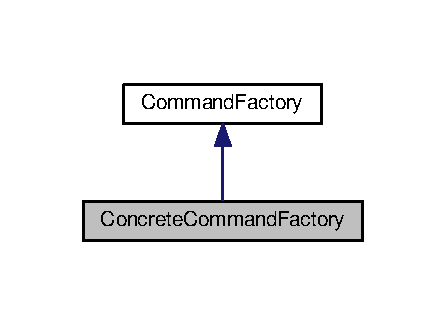
\includegraphics[width=214pt]{classConcreteCommandFactory__inherit__graph}
\end{center}
\end{figure}


Collaboration diagram for Concrete\+Command\+Factory\+:
\nopagebreak
\begin{figure}[H]
\begin{center}
\leavevmode
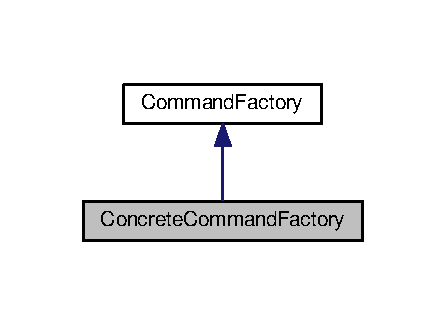
\includegraphics[width=214pt]{classConcreteCommandFactory__coll__graph}
\end{center}
\end{figure}
\subsection*{Public Member Functions}
\begin{DoxyCompactItemize}
\item 
\hyperlink{classConcreteCommandFactory_a03b4c73e1f316aad69c80eb9d6a0b542}{Concrete\+Command\+Factory} ()
\item 
\hyperlink{classConcreteCommandFactory_a3b01f93525176341f57a5869964576d3}{$\sim$\+Concrete\+Command\+Factory} ()
\item 
virtual \hyperlink{classCommand}{Command}$<$ \hyperlink{classExoskeleton}{Exoskeleton} $>$ $\ast$ \hyperlink{classConcreteCommandFactory_a6f7fd417f6959bd0f573ac0127b32631}{create\+Exo\+Command} (\hyperlink{Commands_8hpp_a4a0419b573bf683fef9162331e6ec74e}{Exo\+Command\+ID} id)
\item 
virtual \hyperlink{classCommand}{Command}$<$ \hyperlink{classJoint}{Joint} $>$ $\ast$ \hyperlink{classConcreteCommandFactory_a7ea1fcf9dd01008772c74f1d0fda8253}{create\+Joint\+Command} (\hyperlink{Commands_8hpp_a350356b969551ce1a95947b3cec75d56}{Joint\+Command\+ID} id, \hyperlink{States_8hpp_a26aafbeccd8f356b39e1809f1ab9cfdc}{State\+ID} state, double value)
\item 
virtual \hyperlink{classCommand}{Command}$<$ \hyperlink{classJoint}{Joint} $>$ $\ast$ \hyperlink{classConcreteCommandFactory_a638c86c1d6882d74d1bd53a028235c63}{create\+Joint\+Command} (\hyperlink{Commands_8hpp_a350356b969551ce1a95947b3cec75d56}{Joint\+Command\+ID} id, double, double, double)
\item 
virtual \hyperlink{classCommand}{Command}$<$ \hyperlink{classJoint}{Joint} $>$ $\ast$ \hyperlink{classConcreteCommandFactory_a06e6a5295facfa59451db55af04fc320}{create\+Joint\+Command} (\hyperlink{Commands_8hpp_a350356b969551ce1a95947b3cec75d56}{Joint\+Command\+ID} id, double)
\end{DoxyCompactItemize}


\subsection{Constructor \& Destructor Documentation}
\index{Concrete\+Command\+Factory@{Concrete\+Command\+Factory}!Concrete\+Command\+Factory@{Concrete\+Command\+Factory}}
\index{Concrete\+Command\+Factory@{Concrete\+Command\+Factory}!Concrete\+Command\+Factory@{Concrete\+Command\+Factory}}
\subsubsection[{\texorpdfstring{Concrete\+Command\+Factory()}{ConcreteCommandFactory()}}]{\setlength{\rightskip}{0pt plus 5cm}Concrete\+Command\+Factory\+::\+Concrete\+Command\+Factory (
\begin{DoxyParamCaption}
{}
\end{DoxyParamCaption}
)}\hypertarget{classConcreteCommandFactory_a03b4c73e1f316aad69c80eb9d6a0b542}{}\label{classConcreteCommandFactory_a03b4c73e1f316aad69c80eb9d6a0b542}
\index{Concrete\+Command\+Factory@{Concrete\+Command\+Factory}!````~Concrete\+Command\+Factory@{$\sim$\+Concrete\+Command\+Factory}}
\index{````~Concrete\+Command\+Factory@{$\sim$\+Concrete\+Command\+Factory}!Concrete\+Command\+Factory@{Concrete\+Command\+Factory}}
\subsubsection[{\texorpdfstring{$\sim$\+Concrete\+Command\+Factory()}{~ConcreteCommandFactory()}}]{\setlength{\rightskip}{0pt plus 5cm}Concrete\+Command\+Factory\+::$\sim$\+Concrete\+Command\+Factory (
\begin{DoxyParamCaption}
{}
\end{DoxyParamCaption}
)}\hypertarget{classConcreteCommandFactory_a3b01f93525176341f57a5869964576d3}{}\label{classConcreteCommandFactory_a3b01f93525176341f57a5869964576d3}


\subsection{Member Function Documentation}
\index{Concrete\+Command\+Factory@{Concrete\+Command\+Factory}!create\+Exo\+Command@{create\+Exo\+Command}}
\index{create\+Exo\+Command@{create\+Exo\+Command}!Concrete\+Command\+Factory@{Concrete\+Command\+Factory}}
\subsubsection[{\texorpdfstring{create\+Exo\+Command(\+Exo\+Command\+I\+D id)}{createExoCommand(ExoCommandID id)}}]{\setlength{\rightskip}{0pt plus 5cm}{\bf Command}$<$ {\bf Exoskeleton} $>$ $\ast$ Concrete\+Command\+Factory\+::create\+Exo\+Command (
\begin{DoxyParamCaption}
\item[{{\bf Exo\+Command\+ID}}]{id}
\end{DoxyParamCaption}
)\hspace{0.3cm}{\ttfamily [virtual]}}\hypertarget{classConcreteCommandFactory_a6f7fd417f6959bd0f573ac0127b32631}{}\label{classConcreteCommandFactory_a6f7fd417f6959bd0f573ac0127b32631}


Implements \hyperlink{classCommandFactory_a9cd75aee1d86b52a0c5da5abada1855e}{Command\+Factory}.

\index{Concrete\+Command\+Factory@{Concrete\+Command\+Factory}!create\+Joint\+Command@{create\+Joint\+Command}}
\index{create\+Joint\+Command@{create\+Joint\+Command}!Concrete\+Command\+Factory@{Concrete\+Command\+Factory}}
\subsubsection[{\texorpdfstring{create\+Joint\+Command(\+Joint\+Command\+I\+D id, State\+I\+D state, double value)}{createJointCommand(JointCommandID id, StateID state, double value)}}]{\setlength{\rightskip}{0pt plus 5cm}{\bf Command}$<$ {\bf Joint} $>$ $\ast$ Concrete\+Command\+Factory\+::create\+Joint\+Command (
\begin{DoxyParamCaption}
\item[{{\bf Joint\+Command\+ID}}]{id, }
\item[{{\bf State\+ID}}]{state, }
\item[{double}]{value}
\end{DoxyParamCaption}
)\hspace{0.3cm}{\ttfamily [virtual]}}\hypertarget{classConcreteCommandFactory_a7ea1fcf9dd01008772c74f1d0fda8253}{}\label{classConcreteCommandFactory_a7ea1fcf9dd01008772c74f1d0fda8253}


Implements \hyperlink{classCommandFactory_acdc303aaceaf41b5f53d92e7379d851e}{Command\+Factory}.

\index{Concrete\+Command\+Factory@{Concrete\+Command\+Factory}!create\+Joint\+Command@{create\+Joint\+Command}}
\index{create\+Joint\+Command@{create\+Joint\+Command}!Concrete\+Command\+Factory@{Concrete\+Command\+Factory}}
\subsubsection[{\texorpdfstring{create\+Joint\+Command(\+Joint\+Command\+I\+D id, double, double, double)}{createJointCommand(JointCommandID id, double, double, double)}}]{\setlength{\rightskip}{0pt plus 5cm}{\bf Command}$<$ {\bf Joint} $>$ $\ast$ Concrete\+Command\+Factory\+::create\+Joint\+Command (
\begin{DoxyParamCaption}
\item[{{\bf Joint\+Command\+ID}}]{id, }
\item[{double}]{v1, }
\item[{double}]{v2, }
\item[{double}]{v3}
\end{DoxyParamCaption}
)\hspace{0.3cm}{\ttfamily [virtual]}}\hypertarget{classConcreteCommandFactory_a638c86c1d6882d74d1bd53a028235c63}{}\label{classConcreteCommandFactory_a638c86c1d6882d74d1bd53a028235c63}


Implements \hyperlink{classCommandFactory_af1813c30ede407362ea395c978f24963}{Command\+Factory}.

\index{Concrete\+Command\+Factory@{Concrete\+Command\+Factory}!create\+Joint\+Command@{create\+Joint\+Command}}
\index{create\+Joint\+Command@{create\+Joint\+Command}!Concrete\+Command\+Factory@{Concrete\+Command\+Factory}}
\subsubsection[{\texorpdfstring{create\+Joint\+Command(\+Joint\+Command\+I\+D id, double)}{createJointCommand(JointCommandID id, double)}}]{\setlength{\rightskip}{0pt plus 5cm}{\bf Command}$<$ {\bf Joint} $>$ $\ast$ Concrete\+Command\+Factory\+::create\+Joint\+Command (
\begin{DoxyParamCaption}
\item[{{\bf Joint\+Command\+ID}}]{id, }
\item[{double}]{value}
\end{DoxyParamCaption}
)\hspace{0.3cm}{\ttfamily [virtual]}}\hypertarget{classConcreteCommandFactory_a06e6a5295facfa59451db55af04fc320}{}\label{classConcreteCommandFactory_a06e6a5295facfa59451db55af04fc320}


Implements \hyperlink{classCommandFactory_accade06a34e2d9424ec9765543617e39}{Command\+Factory}.



The documentation for this class was generated from the following files\+:\begin{DoxyCompactItemize}
\item 
\hyperlink{Commands_8hpp}{Commands.\+hpp}\item 
\hyperlink{Commands_8cpp}{Commands.\+cpp}\end{DoxyCompactItemize}

\hypertarget{classControlAlgorithm}{}\section{Control\+Algorithm Class Reference}
\label{classControlAlgorithm}\index{Control\+Algorithm@{Control\+Algorithm}}


{\ttfamily \#include $<$Control\+\_\+\+Algorithms.\+hpp$>$}



Inheritance diagram for Control\+Algorithm\+:\nopagebreak
\begin{figure}[H]
\begin{center}
\leavevmode
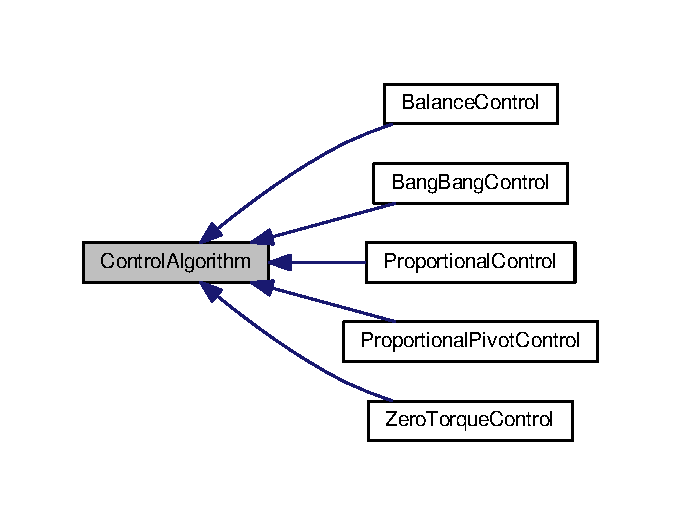
\includegraphics[width=327pt]{classControlAlgorithm__inherit__graph}
\end{center}
\end{figure}
\subsection*{Public Member Functions}
\begin{DoxyCompactItemize}
\item 
\hyperlink{classControlAlgorithm_a91089205780f22d25043b8d01b64323a}{Control\+Algorithm} (\hyperlink{States_8hpp_a26aafbeccd8f356b39e1809f1ab9cfdc}{State\+ID} state\+\_\+id)
\item 
virtual \hyperlink{classControlAlgorithm_a2c0a0a5a73afcbbdfdb1f1fc3c9408fd}{$\sim$\+Control\+Algorithm} ()
\item 
void \hyperlink{classControlAlgorithm_a6b0718c1b8eb993e2d97418e2758adb9}{set\+Previous\+Control\+Algorithm} (\hyperlink{classControlAlgorithm}{Control\+Algorithm} $\ast$control\+\_\+algorithm)
\item 
void \hyperlink{classControlAlgorithm_a81403fa6713bb56859df497503a6a09f}{delete\+Algorithm\+State\+Machine} ()
\item 
virtual void \hyperlink{classControlAlgorithm_ae94b3eefb4b06213e27ef61ee3e9876b}{set\+Desired\+Setpoint} (double setpoint)
\item 
virtual double \hyperlink{classControlAlgorithm_ac9b448583431a037bc8636872ee9bfb3}{get\+Desired\+Setpoint} ()
\item 
virtual double \hyperlink{classControlAlgorithm_a5fd58cfd5b601dc4556170bb620ea7f5}{get\+Shaping\+Iterations} ()
\item 
virtual void \hyperlink{classControlAlgorithm_afb67f383de5f6e85c7a7b8e711953c0e}{set\+Shaping\+Iterations} (double iterations)
\item 
virtual void \hyperlink{classControlAlgorithm_a0da6d49c48afb6df7c1bc4bad4e5a3f0}{activate} ()
\item 
virtual double \hyperlink{classControlAlgorithm_a038ebc5f26c3ae460f04eaf7f0dc0e29}{get\+Setpoint} (\hyperlink{classSensorReport}{Sensor\+Report} $\ast$report)=0
\item 
virtual bool \hyperlink{classControlAlgorithm_ac9e2b1e3677e4ace7071c540fe035ae4}{use\+Shaping\+Function} ()=0
\item 
virtual \hyperlink{Control__Algorithms_8hpp_afda28772870dd56f60cd7a301337392c}{Control\+Algorithm\+Type} \hyperlink{classControlAlgorithm_a432f51282dfe836befccdecaaa9741c5}{get\+Type} ()=0
\item 
virtual void \hyperlink{classControlAlgorithm_a154061241e21f6f7feb7165eda91bf15}{set\+To\+Zero} ()
\item 
virtual void \hyperlink{classControlAlgorithm_a9e64d8fb3fb40414adef533a0914c8fc}{reset} ()
\item 
virtual void \hyperlink{classControlAlgorithm_a694627bbf7d01f2c7f62d83e672b9231}{reset\+Starting\+Parameters} ()
\item 
virtual void \hyperlink{classControlAlgorithm_ad4cee63394f06ffa2227ece3579b9b05}{set\+Gain} (double \hyperlink{classControlAlgorithm_a2ac40220b20a6bf9f1ee0665138467a5}{gain})
\item 
virtual \hyperlink{States_8hpp_a26aafbeccd8f356b39e1809f1ab9cfdc}{State\+ID} \hyperlink{classControlAlgorithm_a68ec2395b0ea38776d38e219b16dc827}{get\+State\+ID} ()
\item 
virtual \hyperlink{classControlAlgorithm}{Control\+Algorithm} $\ast$ \hyperlink{classControlAlgorithm_acc910803a006526921450cfd66467d2e}{get\+Next\+Algorithm} ()
\end{DoxyCompactItemize}
\subsection*{Protected Member Functions}
\begin{DoxyCompactItemize}
\item 
double \hyperlink{classControlAlgorithm_a5433d86e863ff01f0fc990a955afb893}{get\+Activation\+Percent} ()
\item 
double \hyperlink{classControlAlgorithm_a7cf1dc233469cac50bec27020ca3ddf3}{clamp\+\_\+setpoint} (double raw\+\_\+setpoint)
\end{DoxyCompactItemize}
\subsection*{Protected Attributes}
\begin{DoxyCompactItemize}
\item 
double \hyperlink{classControlAlgorithm_a2ac40220b20a6bf9f1ee0665138467a5}{gain}
\item 
double \hyperlink{classControlAlgorithm_aabbb3a42a32c1996b22b0e15bdb4ff1b}{desired\+\_\+setpoint}
\item 
double \hyperlink{classControlAlgorithm_adc4574602d459aca5b9320937bc102b1}{previous\+\_\+desired\+\_\+setpoint}
\item 
double \hyperlink{classControlAlgorithm_a02ba55f15705474b47a0635b027a7b44}{used\+\_\+setpoint}
\item 
int \hyperlink{classControlAlgorithm_ac1a0dc23fe7d2cac2301de1d7e95c357}{shaping\+\_\+iteration\+\_\+threshold}
\end{DoxyCompactItemize}


\subsection{Constructor \& Destructor Documentation}
\index{Control\+Algorithm@{Control\+Algorithm}!Control\+Algorithm@{Control\+Algorithm}}
\index{Control\+Algorithm@{Control\+Algorithm}!Control\+Algorithm@{Control\+Algorithm}}
\subsubsection[{\texorpdfstring{Control\+Algorithm(\+State\+I\+D state\+\_\+id)}{ControlAlgorithm(StateID state_id)}}]{\setlength{\rightskip}{0pt plus 5cm}Control\+Algorithm\+::\+Control\+Algorithm (
\begin{DoxyParamCaption}
\item[{{\bf State\+ID}}]{state\+\_\+id}
\end{DoxyParamCaption}
)}\hypertarget{classControlAlgorithm_a91089205780f22d25043b8d01b64323a}{}\label{classControlAlgorithm_a91089205780f22d25043b8d01b64323a}
\index{Control\+Algorithm@{Control\+Algorithm}!````~Control\+Algorithm@{$\sim$\+Control\+Algorithm}}
\index{````~Control\+Algorithm@{$\sim$\+Control\+Algorithm}!Control\+Algorithm@{Control\+Algorithm}}
\subsubsection[{\texorpdfstring{$\sim$\+Control\+Algorithm()}{~ControlAlgorithm()}}]{\setlength{\rightskip}{0pt plus 5cm}Control\+Algorithm\+::$\sim$\+Control\+Algorithm (
\begin{DoxyParamCaption}
{}
\end{DoxyParamCaption}
)\hspace{0.3cm}{\ttfamily [virtual]}}\hypertarget{classControlAlgorithm_a2c0a0a5a73afcbbdfdb1f1fc3c9408fd}{}\label{classControlAlgorithm_a2c0a0a5a73afcbbdfdb1f1fc3c9408fd}


\subsection{Member Function Documentation}
\index{Control\+Algorithm@{Control\+Algorithm}!activate@{activate}}
\index{activate@{activate}!Control\+Algorithm@{Control\+Algorithm}}
\subsubsection[{\texorpdfstring{activate()}{activate()}}]{\setlength{\rightskip}{0pt plus 5cm}void Control\+Algorithm\+::activate (
\begin{DoxyParamCaption}
{}
\end{DoxyParamCaption}
)\hspace{0.3cm}{\ttfamily [virtual]}}\hypertarget{classControlAlgorithm_a0da6d49c48afb6df7c1bc4bad4e5a3f0}{}\label{classControlAlgorithm_a0da6d49c48afb6df7c1bc4bad4e5a3f0}


Reimplemented in \hyperlink{classBangBangControl_a9e8e9d63842c9640212993f8ba02e4a1}{Bang\+Bang\+Control}.

\index{Control\+Algorithm@{Control\+Algorithm}!clamp\+\_\+setpoint@{clamp\+\_\+setpoint}}
\index{clamp\+\_\+setpoint@{clamp\+\_\+setpoint}!Control\+Algorithm@{Control\+Algorithm}}
\subsubsection[{\texorpdfstring{clamp\+\_\+setpoint(double raw\+\_\+setpoint)}{clamp_setpoint(double raw_setpoint)}}]{\setlength{\rightskip}{0pt plus 5cm}double Control\+Algorithm\+::clamp\+\_\+setpoint (
\begin{DoxyParamCaption}
\item[{double}]{raw\+\_\+setpoint}
\end{DoxyParamCaption}
)\hspace{0.3cm}{\ttfamily [protected]}}\hypertarget{classControlAlgorithm_a7cf1dc233469cac50bec27020ca3ddf3}{}\label{classControlAlgorithm_a7cf1dc233469cac50bec27020ca3ddf3}
\index{Control\+Algorithm@{Control\+Algorithm}!delete\+Algorithm\+State\+Machine@{delete\+Algorithm\+State\+Machine}}
\index{delete\+Algorithm\+State\+Machine@{delete\+Algorithm\+State\+Machine}!Control\+Algorithm@{Control\+Algorithm}}
\subsubsection[{\texorpdfstring{delete\+Algorithm\+State\+Machine()}{deleteAlgorithmStateMachine()}}]{\setlength{\rightskip}{0pt plus 5cm}void Control\+Algorithm\+::delete\+Algorithm\+State\+Machine (
\begin{DoxyParamCaption}
{}
\end{DoxyParamCaption}
)}\hypertarget{classControlAlgorithm_a81403fa6713bb56859df497503a6a09f}{}\label{classControlAlgorithm_a81403fa6713bb56859df497503a6a09f}
\index{Control\+Algorithm@{Control\+Algorithm}!get\+Activation\+Percent@{get\+Activation\+Percent}}
\index{get\+Activation\+Percent@{get\+Activation\+Percent}!Control\+Algorithm@{Control\+Algorithm}}
\subsubsection[{\texorpdfstring{get\+Activation\+Percent()}{getActivationPercent()}}]{\setlength{\rightskip}{0pt plus 5cm}double Control\+Algorithm\+::get\+Activation\+Percent (
\begin{DoxyParamCaption}
{}
\end{DoxyParamCaption}
)\hspace{0.3cm}{\ttfamily [protected]}}\hypertarget{classControlAlgorithm_a5433d86e863ff01f0fc990a955afb893}{}\label{classControlAlgorithm_a5433d86e863ff01f0fc990a955afb893}
\index{Control\+Algorithm@{Control\+Algorithm}!get\+Desired\+Setpoint@{get\+Desired\+Setpoint}}
\index{get\+Desired\+Setpoint@{get\+Desired\+Setpoint}!Control\+Algorithm@{Control\+Algorithm}}
\subsubsection[{\texorpdfstring{get\+Desired\+Setpoint()}{getDesiredSetpoint()}}]{\setlength{\rightskip}{0pt plus 5cm}double Control\+Algorithm\+::get\+Desired\+Setpoint (
\begin{DoxyParamCaption}
{}
\end{DoxyParamCaption}
)\hspace{0.3cm}{\ttfamily [virtual]}}\hypertarget{classControlAlgorithm_ac9b448583431a037bc8636872ee9bfb3}{}\label{classControlAlgorithm_ac9b448583431a037bc8636872ee9bfb3}
\index{Control\+Algorithm@{Control\+Algorithm}!get\+Next\+Algorithm@{get\+Next\+Algorithm}}
\index{get\+Next\+Algorithm@{get\+Next\+Algorithm}!Control\+Algorithm@{Control\+Algorithm}}
\subsubsection[{\texorpdfstring{get\+Next\+Algorithm()}{getNextAlgorithm()}}]{\setlength{\rightskip}{0pt plus 5cm}{\bf Control\+Algorithm} $\ast$ Control\+Algorithm\+::get\+Next\+Algorithm (
\begin{DoxyParamCaption}
{}
\end{DoxyParamCaption}
)\hspace{0.3cm}{\ttfamily [virtual]}}\hypertarget{classControlAlgorithm_acc910803a006526921450cfd66467d2e}{}\label{classControlAlgorithm_acc910803a006526921450cfd66467d2e}
\index{Control\+Algorithm@{Control\+Algorithm}!get\+Setpoint@{get\+Setpoint}}
\index{get\+Setpoint@{get\+Setpoint}!Control\+Algorithm@{Control\+Algorithm}}
\subsubsection[{\texorpdfstring{get\+Setpoint(\+Sensor\+Report $\ast$report)=0}{getSetpoint(SensorReport *report)=0}}]{\setlength{\rightskip}{0pt plus 5cm}virtual double Control\+Algorithm\+::get\+Setpoint (
\begin{DoxyParamCaption}
\item[{{\bf Sensor\+Report} $\ast$}]{report}
\end{DoxyParamCaption}
)\hspace{0.3cm}{\ttfamily [pure virtual]}}\hypertarget{classControlAlgorithm_a038ebc5f26c3ae460f04eaf7f0dc0e29}{}\label{classControlAlgorithm_a038ebc5f26c3ae460f04eaf7f0dc0e29}


Implemented in \hyperlink{classProportionalPivotControl_ae8094c36c9df1e1221dcb9c9bcbdf0b2}{Proportional\+Pivot\+Control}, \hyperlink{classProportionalControl_ae550aa587d3eae22a039aaf1ce13d406}{Proportional\+Control}, \hyperlink{classBalanceControl_ab7bc00e4dea77cf34c02ef1f4bb2feec}{Balance\+Control}, \hyperlink{classBangBangControl_a6fd492fbf7d9e255ef82c85f426cb794}{Bang\+Bang\+Control}, and \hyperlink{classZeroTorqueControl_a2542dc5dfbb6508d653af5fab5c1c537}{Zero\+Torque\+Control}.

\index{Control\+Algorithm@{Control\+Algorithm}!get\+Shaping\+Iterations@{get\+Shaping\+Iterations}}
\index{get\+Shaping\+Iterations@{get\+Shaping\+Iterations}!Control\+Algorithm@{Control\+Algorithm}}
\subsubsection[{\texorpdfstring{get\+Shaping\+Iterations()}{getShapingIterations()}}]{\setlength{\rightskip}{0pt plus 5cm}double Control\+Algorithm\+::get\+Shaping\+Iterations (
\begin{DoxyParamCaption}
{}
\end{DoxyParamCaption}
)\hspace{0.3cm}{\ttfamily [virtual]}}\hypertarget{classControlAlgorithm_a5fd58cfd5b601dc4556170bb620ea7f5}{}\label{classControlAlgorithm_a5fd58cfd5b601dc4556170bb620ea7f5}


Reimplemented in \hyperlink{classBalanceControl_a0ba1c9cd74a877eb0f748325763c02e4}{Balance\+Control}.

\index{Control\+Algorithm@{Control\+Algorithm}!get\+State\+ID@{get\+State\+ID}}
\index{get\+State\+ID@{get\+State\+ID}!Control\+Algorithm@{Control\+Algorithm}}
\subsubsection[{\texorpdfstring{get\+State\+I\+D()}{getStateID()}}]{\setlength{\rightskip}{0pt plus 5cm}{\bf State\+ID} Control\+Algorithm\+::get\+State\+ID (
\begin{DoxyParamCaption}
{}
\end{DoxyParamCaption}
)\hspace{0.3cm}{\ttfamily [virtual]}}\hypertarget{classControlAlgorithm_a68ec2395b0ea38776d38e219b16dc827}{}\label{classControlAlgorithm_a68ec2395b0ea38776d38e219b16dc827}
\index{Control\+Algorithm@{Control\+Algorithm}!get\+Type@{get\+Type}}
\index{get\+Type@{get\+Type}!Control\+Algorithm@{Control\+Algorithm}}
\subsubsection[{\texorpdfstring{get\+Type()=0}{getType()=0}}]{\setlength{\rightskip}{0pt plus 5cm}virtual {\bf Control\+Algorithm\+Type} Control\+Algorithm\+::get\+Type (
\begin{DoxyParamCaption}
{}
\end{DoxyParamCaption}
)\hspace{0.3cm}{\ttfamily [pure virtual]}}\hypertarget{classControlAlgorithm_a432f51282dfe836befccdecaaa9741c5}{}\label{classControlAlgorithm_a432f51282dfe836befccdecaaa9741c5}


Implemented in \hyperlink{classProportionalPivotControl_acf9ea5348039c173e06328009eb96309}{Proportional\+Pivot\+Control}, \hyperlink{classProportionalControl_a4332cd13fdee5d347c85685bdd307dd9}{Proportional\+Control}, \hyperlink{classBalanceControl_a8314d9b67c800b7e0ca2be07ae7e1343}{Balance\+Control}, \hyperlink{classBangBangControl_a240b1a40e88fdcd4e943319dd83654d0}{Bang\+Bang\+Control}, and \hyperlink{classZeroTorqueControl_acfc9e976d8c2453e866f09c98843f6ab}{Zero\+Torque\+Control}.

\index{Control\+Algorithm@{Control\+Algorithm}!reset@{reset}}
\index{reset@{reset}!Control\+Algorithm@{Control\+Algorithm}}
\subsubsection[{\texorpdfstring{reset()}{reset()}}]{\setlength{\rightskip}{0pt plus 5cm}void Control\+Algorithm\+::reset (
\begin{DoxyParamCaption}
{}
\end{DoxyParamCaption}
)\hspace{0.3cm}{\ttfamily [virtual]}}\hypertarget{classControlAlgorithm_a9e64d8fb3fb40414adef533a0914c8fc}{}\label{classControlAlgorithm_a9e64d8fb3fb40414adef533a0914c8fc}
\index{Control\+Algorithm@{Control\+Algorithm}!reset\+Starting\+Parameters@{reset\+Starting\+Parameters}}
\index{reset\+Starting\+Parameters@{reset\+Starting\+Parameters}!Control\+Algorithm@{Control\+Algorithm}}
\subsubsection[{\texorpdfstring{reset\+Starting\+Parameters()}{resetStartingParameters()}}]{\setlength{\rightskip}{0pt plus 5cm}void Control\+Algorithm\+::reset\+Starting\+Parameters (
\begin{DoxyParamCaption}
{}
\end{DoxyParamCaption}
)\hspace{0.3cm}{\ttfamily [virtual]}}\hypertarget{classControlAlgorithm_a694627bbf7d01f2c7f62d83e672b9231}{}\label{classControlAlgorithm_a694627bbf7d01f2c7f62d83e672b9231}
\index{Control\+Algorithm@{Control\+Algorithm}!set\+Desired\+Setpoint@{set\+Desired\+Setpoint}}
\index{set\+Desired\+Setpoint@{set\+Desired\+Setpoint}!Control\+Algorithm@{Control\+Algorithm}}
\subsubsection[{\texorpdfstring{set\+Desired\+Setpoint(double setpoint)}{setDesiredSetpoint(double setpoint)}}]{\setlength{\rightskip}{0pt plus 5cm}void Control\+Algorithm\+::set\+Desired\+Setpoint (
\begin{DoxyParamCaption}
\item[{double}]{setpoint}
\end{DoxyParamCaption}
)\hspace{0.3cm}{\ttfamily [virtual]}}\hypertarget{classControlAlgorithm_ae94b3eefb4b06213e27ef61ee3e9876b}{}\label{classControlAlgorithm_ae94b3eefb4b06213e27ef61ee3e9876b}
\index{Control\+Algorithm@{Control\+Algorithm}!set\+Gain@{set\+Gain}}
\index{set\+Gain@{set\+Gain}!Control\+Algorithm@{Control\+Algorithm}}
\subsubsection[{\texorpdfstring{set\+Gain(double gain)}{setGain(double gain)}}]{\setlength{\rightskip}{0pt plus 5cm}void Control\+Algorithm\+::set\+Gain (
\begin{DoxyParamCaption}
\item[{double}]{gain}
\end{DoxyParamCaption}
)\hspace{0.3cm}{\ttfamily [virtual]}}\hypertarget{classControlAlgorithm_ad4cee63394f06ffa2227ece3579b9b05}{}\label{classControlAlgorithm_ad4cee63394f06ffa2227ece3579b9b05}
\index{Control\+Algorithm@{Control\+Algorithm}!set\+Previous\+Control\+Algorithm@{set\+Previous\+Control\+Algorithm}}
\index{set\+Previous\+Control\+Algorithm@{set\+Previous\+Control\+Algorithm}!Control\+Algorithm@{Control\+Algorithm}}
\subsubsection[{\texorpdfstring{set\+Previous\+Control\+Algorithm(\+Control\+Algorithm $\ast$control\+\_\+algorithm)}{setPreviousControlAlgorithm(ControlAlgorithm *control_algorithm)}}]{\setlength{\rightskip}{0pt plus 5cm}void Control\+Algorithm\+::set\+Previous\+Control\+Algorithm (
\begin{DoxyParamCaption}
\item[{{\bf Control\+Algorithm} $\ast$}]{control\+\_\+algorithm}
\end{DoxyParamCaption}
)}\hypertarget{classControlAlgorithm_a6b0718c1b8eb993e2d97418e2758adb9}{}\label{classControlAlgorithm_a6b0718c1b8eb993e2d97418e2758adb9}
\index{Control\+Algorithm@{Control\+Algorithm}!set\+Shaping\+Iterations@{set\+Shaping\+Iterations}}
\index{set\+Shaping\+Iterations@{set\+Shaping\+Iterations}!Control\+Algorithm@{Control\+Algorithm}}
\subsubsection[{\texorpdfstring{set\+Shaping\+Iterations(double iterations)}{setShapingIterations(double iterations)}}]{\setlength{\rightskip}{0pt plus 5cm}void Control\+Algorithm\+::set\+Shaping\+Iterations (
\begin{DoxyParamCaption}
\item[{double}]{iterations}
\end{DoxyParamCaption}
)\hspace{0.3cm}{\ttfamily [virtual]}}\hypertarget{classControlAlgorithm_afb67f383de5f6e85c7a7b8e711953c0e}{}\label{classControlAlgorithm_afb67f383de5f6e85c7a7b8e711953c0e}
\index{Control\+Algorithm@{Control\+Algorithm}!set\+To\+Zero@{set\+To\+Zero}}
\index{set\+To\+Zero@{set\+To\+Zero}!Control\+Algorithm@{Control\+Algorithm}}
\subsubsection[{\texorpdfstring{set\+To\+Zero()}{setToZero()}}]{\setlength{\rightskip}{0pt plus 5cm}void Control\+Algorithm\+::set\+To\+Zero (
\begin{DoxyParamCaption}
{}
\end{DoxyParamCaption}
)\hspace{0.3cm}{\ttfamily [virtual]}}\hypertarget{classControlAlgorithm_a154061241e21f6f7feb7165eda91bf15}{}\label{classControlAlgorithm_a154061241e21f6f7feb7165eda91bf15}
\index{Control\+Algorithm@{Control\+Algorithm}!use\+Shaping\+Function@{use\+Shaping\+Function}}
\index{use\+Shaping\+Function@{use\+Shaping\+Function}!Control\+Algorithm@{Control\+Algorithm}}
\subsubsection[{\texorpdfstring{use\+Shaping\+Function()=0}{useShapingFunction()=0}}]{\setlength{\rightskip}{0pt plus 5cm}virtual bool Control\+Algorithm\+::use\+Shaping\+Function (
\begin{DoxyParamCaption}
{}
\end{DoxyParamCaption}
)\hspace{0.3cm}{\ttfamily [pure virtual]}}\hypertarget{classControlAlgorithm_ac9e2b1e3677e4ace7071c540fe035ae4}{}\label{classControlAlgorithm_ac9e2b1e3677e4ace7071c540fe035ae4}


Implemented in \hyperlink{classProportionalPivotControl_a464adb4fb2d222490f1916671709cc78}{Proportional\+Pivot\+Control}, \hyperlink{classProportionalControl_aa3fcb8e6b28f839f6793a15f11f3ff2b}{Proportional\+Control}, \hyperlink{classBalanceControl_a9761db9b15bb15e6d2f19f6d2243c888}{Balance\+Control}, \hyperlink{classBangBangControl_af85b04c727a5e11c1d54d0a15d5ca64c}{Bang\+Bang\+Control}, and \hyperlink{classZeroTorqueControl_a62afa8c85150e54395171254ac8b90ef}{Zero\+Torque\+Control}.



\subsection{Member Data Documentation}
\index{Control\+Algorithm@{Control\+Algorithm}!desired\+\_\+setpoint@{desired\+\_\+setpoint}}
\index{desired\+\_\+setpoint@{desired\+\_\+setpoint}!Control\+Algorithm@{Control\+Algorithm}}
\subsubsection[{\texorpdfstring{desired\+\_\+setpoint}{desired_setpoint}}]{\setlength{\rightskip}{0pt plus 5cm}double Control\+Algorithm\+::desired\+\_\+setpoint\hspace{0.3cm}{\ttfamily [protected]}}\hypertarget{classControlAlgorithm_aabbb3a42a32c1996b22b0e15bdb4ff1b}{}\label{classControlAlgorithm_aabbb3a42a32c1996b22b0e15bdb4ff1b}
\index{Control\+Algorithm@{Control\+Algorithm}!gain@{gain}}
\index{gain@{gain}!Control\+Algorithm@{Control\+Algorithm}}
\subsubsection[{\texorpdfstring{gain}{gain}}]{\setlength{\rightskip}{0pt plus 5cm}double Control\+Algorithm\+::gain\hspace{0.3cm}{\ttfamily [protected]}}\hypertarget{classControlAlgorithm_a2ac40220b20a6bf9f1ee0665138467a5}{}\label{classControlAlgorithm_a2ac40220b20a6bf9f1ee0665138467a5}
\index{Control\+Algorithm@{Control\+Algorithm}!previous\+\_\+desired\+\_\+setpoint@{previous\+\_\+desired\+\_\+setpoint}}
\index{previous\+\_\+desired\+\_\+setpoint@{previous\+\_\+desired\+\_\+setpoint}!Control\+Algorithm@{Control\+Algorithm}}
\subsubsection[{\texorpdfstring{previous\+\_\+desired\+\_\+setpoint}{previous_desired_setpoint}}]{\setlength{\rightskip}{0pt plus 5cm}double Control\+Algorithm\+::previous\+\_\+desired\+\_\+setpoint\hspace{0.3cm}{\ttfamily [protected]}}\hypertarget{classControlAlgorithm_adc4574602d459aca5b9320937bc102b1}{}\label{classControlAlgorithm_adc4574602d459aca5b9320937bc102b1}
\index{Control\+Algorithm@{Control\+Algorithm}!shaping\+\_\+iteration\+\_\+threshold@{shaping\+\_\+iteration\+\_\+threshold}}
\index{shaping\+\_\+iteration\+\_\+threshold@{shaping\+\_\+iteration\+\_\+threshold}!Control\+Algorithm@{Control\+Algorithm}}
\subsubsection[{\texorpdfstring{shaping\+\_\+iteration\+\_\+threshold}{shaping_iteration_threshold}}]{\setlength{\rightskip}{0pt plus 5cm}int Control\+Algorithm\+::shaping\+\_\+iteration\+\_\+threshold\hspace{0.3cm}{\ttfamily [protected]}}\hypertarget{classControlAlgorithm_ac1a0dc23fe7d2cac2301de1d7e95c357}{}\label{classControlAlgorithm_ac1a0dc23fe7d2cac2301de1d7e95c357}
\index{Control\+Algorithm@{Control\+Algorithm}!used\+\_\+setpoint@{used\+\_\+setpoint}}
\index{used\+\_\+setpoint@{used\+\_\+setpoint}!Control\+Algorithm@{Control\+Algorithm}}
\subsubsection[{\texorpdfstring{used\+\_\+setpoint}{used_setpoint}}]{\setlength{\rightskip}{0pt plus 5cm}double Control\+Algorithm\+::used\+\_\+setpoint\hspace{0.3cm}{\ttfamily [protected]}}\hypertarget{classControlAlgorithm_a02ba55f15705474b47a0635b027a7b44}{}\label{classControlAlgorithm_a02ba55f15705474b47a0635b027a7b44}


The documentation for this class was generated from the following files\+:\begin{DoxyCompactItemize}
\item 
\hyperlink{Control__Algorithms_8hpp}{Control\+\_\+\+Algorithms.\+hpp}\item 
\hyperlink{Control__Algorithms_8cpp}{Control\+\_\+\+Algorithms.\+cpp}\end{DoxyCompactItemize}

\hypertarget{classControlModule}{}\section{Control\+Module Class Reference}
\label{classControlModule}\index{Control\+Module@{Control\+Module}}


{\ttfamily \#include $<$Control\+\_\+\+Module.\+hpp$>$}

\subsection*{Public Member Functions}
\begin{DoxyCompactItemize}
\item 
\hyperlink{classControlModule_a4314676da13e7c4f658d042bb8035f38}{Control\+Module} (\hyperlink{classControlAlgorithm}{Control\+Algorithm} $\ast$state\+\_\+machine, \hyperlink{States_8hpp_a26aafbeccd8f356b39e1809f1ab9cfdc}{State\+ID} starting\+\_\+state)
\item 
\hyperlink{classControlModule_ade41c6a3ce7c8e4df978c611bc0d9fa8}{$\sim$\+Control\+Module} ()
\item 
void \hyperlink{classControlModule_aaefdbef057adda0ee6ac86225b974736}{set\+Control\+State\+Machine} (\hyperlink{classControlAlgorithm}{Control\+Algorithm} $\ast$state\+\_\+machine, \hyperlink{States_8hpp_a26aafbeccd8f356b39e1809f1ab9cfdc}{State\+ID} starting\+\_\+state)
\item 
void \hyperlink{classControlModule_a02cb4c34e322b292577cb31182ea52a4}{set\+Algorithm\+Desired\+Setpoint} (\hyperlink{States_8hpp_a26aafbeccd8f356b39e1809f1ab9cfdc}{State\+ID} state, double setpoint)
\item 
double \hyperlink{classControlModule_a39e3f7c7bf68975a66ebde771be0fe1e}{get\+Algorithm\+Desired\+Setpoint} (\hyperlink{States_8hpp_a26aafbeccd8f356b39e1809f1ab9cfdc}{State\+ID} state)
\item 
void \hyperlink{classControlModule_a12080a39a838b7d527d9c0908483cd22}{set\+To\+Zero} ()
\item 
void \hyperlink{classControlModule_abe605807dc1f58e4bdea40e49f6f3b12}{set\+Desired\+Setpoint} (double setpoint)
\item 
void \hyperlink{classControlModule_a6698998f891f6243cfbf9590ee72c3d7}{change\+State} (\hyperlink{States_8hpp_a26aafbeccd8f356b39e1809f1ab9cfdc}{State\+ID} state\+\_\+id)
\item 
double \hyperlink{classControlModule_aa3c64f7fe97d2cc67c761770fd7a134a}{get\+Control\+Adjustment} (double torque\+\_\+input, \hyperlink{classSensorReport}{Sensor\+Report} $\ast$report)
\item 
void \hyperlink{classControlModule_a19b05cacdc40d708d14c00c5a41142b5}{reset\+Starting\+Parameters} ()
\item 
void \hyperlink{classControlModule_aee5754ea42ce1a9bae086da2f2ca029c}{adjust\+Shaping\+For\+Time} (double planter\+\_\+time)
\item 
void \hyperlink{classControlModule_affa4c0234bf7883a33b159efb3b1f2dc}{change\+Control} (\hyperlink{States_8hpp_a26aafbeccd8f356b39e1809f1ab9cfdc}{State\+ID} state\+\_\+id)
\item 
void \hyperlink{classControlModule_a5b296b6354c48e2252e89c83b2399475}{update\+K\+F\+P\+I\+D\+Error} (double torque)
\item 
void \hyperlink{classControlModule_a8159eb15ae67becab77531e6080fc6fd}{apply\+Auto\+KF} ()
\item 
double \hyperlink{classControlModule_ac66e25402eeae49116dbea00534a4a22}{get\+Last\+Setpoint} ()
\item 
void \hyperlink{classControlModule_a143642ed467c636cab3c8bf25bbe354e}{get\+Pid} (double $\ast$pid)
\item 
void \hyperlink{classControlModule_a8bab02465545b89adb46b6ccc42ead81}{set\+Pid} (double \hyperlink{Parameters_8hpp_ad1ae3be971981842496c18dabdd2e4c1}{p}, double i, double d)
\item 
double \hyperlink{classControlModule_a36a061b2c4c6ccfb4eb9a8f8bd577b89}{get\+Kf} ()
\item 
void \hyperlink{classControlModule_af2b5bb6c70236be1b00b43c0c357f07d}{set\+Kf} (double kf)
\item 
double \hyperlink{classControlModule_a431dca55f4fcc7935138955183fb5be6}{get\+Smoothing\+Param} (\hyperlink{States_8hpp_a26aafbeccd8f356b39e1809f1ab9cfdc}{State\+ID} state)
\item 
void \hyperlink{classControlModule_a5ebcc624316224590d8cf7856b7283a8}{set\+Smoothing\+Param} (\hyperlink{States_8hpp_a26aafbeccd8f356b39e1809f1ab9cfdc}{State\+ID} state, double param)
\end{DoxyCompactItemize}


\subsection{Constructor \& Destructor Documentation}
\index{Control\+Module@{Control\+Module}!Control\+Module@{Control\+Module}}
\index{Control\+Module@{Control\+Module}!Control\+Module@{Control\+Module}}
\subsubsection[{\texorpdfstring{Control\+Module(\+Control\+Algorithm $\ast$state\+\_\+machine, State\+I\+D starting\+\_\+state)}{ControlModule(ControlAlgorithm *state_machine, StateID starting_state)}}]{\setlength{\rightskip}{0pt plus 5cm}Control\+Module\+::\+Control\+Module (
\begin{DoxyParamCaption}
\item[{{\bf Control\+Algorithm} $\ast$}]{state\+\_\+machine, }
\item[{{\bf State\+ID}}]{starting\+\_\+state}
\end{DoxyParamCaption}
)}\hypertarget{classControlModule_a4314676da13e7c4f658d042bb8035f38}{}\label{classControlModule_a4314676da13e7c4f658d042bb8035f38}
\index{Control\+Module@{Control\+Module}!````~Control\+Module@{$\sim$\+Control\+Module}}
\index{````~Control\+Module@{$\sim$\+Control\+Module}!Control\+Module@{Control\+Module}}
\subsubsection[{\texorpdfstring{$\sim$\+Control\+Module()}{~ControlModule()}}]{\setlength{\rightskip}{0pt plus 5cm}Control\+Module\+::$\sim$\+Control\+Module (
\begin{DoxyParamCaption}
{}
\end{DoxyParamCaption}
)}\hypertarget{classControlModule_ade41c6a3ce7c8e4df978c611bc0d9fa8}{}\label{classControlModule_ade41c6a3ce7c8e4df978c611bc0d9fa8}


\subsection{Member Function Documentation}
\index{Control\+Module@{Control\+Module}!adjust\+Shaping\+For\+Time@{adjust\+Shaping\+For\+Time}}
\index{adjust\+Shaping\+For\+Time@{adjust\+Shaping\+For\+Time}!Control\+Module@{Control\+Module}}
\subsubsection[{\texorpdfstring{adjust\+Shaping\+For\+Time(double planter\+\_\+time)}{adjustShapingForTime(double planter_time)}}]{\setlength{\rightskip}{0pt plus 5cm}void Control\+Module\+::adjust\+Shaping\+For\+Time (
\begin{DoxyParamCaption}
\item[{double}]{planter\+\_\+time}
\end{DoxyParamCaption}
)}\hypertarget{classControlModule_aee5754ea42ce1a9bae086da2f2ca029c}{}\label{classControlModule_aee5754ea42ce1a9bae086da2f2ca029c}
\index{Control\+Module@{Control\+Module}!apply\+Auto\+KF@{apply\+Auto\+KF}}
\index{apply\+Auto\+KF@{apply\+Auto\+KF}!Control\+Module@{Control\+Module}}
\subsubsection[{\texorpdfstring{apply\+Auto\+K\+F()}{applyAutoKF()}}]{\setlength{\rightskip}{0pt plus 5cm}void Control\+Module\+::apply\+Auto\+KF (
\begin{DoxyParamCaption}
{}
\end{DoxyParamCaption}
)}\hypertarget{classControlModule_a8159eb15ae67becab77531e6080fc6fd}{}\label{classControlModule_a8159eb15ae67becab77531e6080fc6fd}
\index{Control\+Module@{Control\+Module}!change\+Control@{change\+Control}}
\index{change\+Control@{change\+Control}!Control\+Module@{Control\+Module}}
\subsubsection[{\texorpdfstring{change\+Control(\+State\+I\+D state\+\_\+id)}{changeControl(StateID state_id)}}]{\setlength{\rightskip}{0pt plus 5cm}void Control\+Module\+::change\+Control (
\begin{DoxyParamCaption}
\item[{{\bf State\+ID}}]{state\+\_\+id}
\end{DoxyParamCaption}
)}\hypertarget{classControlModule_affa4c0234bf7883a33b159efb3b1f2dc}{}\label{classControlModule_affa4c0234bf7883a33b159efb3b1f2dc}
\index{Control\+Module@{Control\+Module}!change\+State@{change\+State}}
\index{change\+State@{change\+State}!Control\+Module@{Control\+Module}}
\subsubsection[{\texorpdfstring{change\+State(\+State\+I\+D state\+\_\+id)}{changeState(StateID state_id)}}]{\setlength{\rightskip}{0pt plus 5cm}void Control\+Module\+::change\+State (
\begin{DoxyParamCaption}
\item[{{\bf State\+ID}}]{state\+\_\+id}
\end{DoxyParamCaption}
)}\hypertarget{classControlModule_a6698998f891f6243cfbf9590ee72c3d7}{}\label{classControlModule_a6698998f891f6243cfbf9590ee72c3d7}
\index{Control\+Module@{Control\+Module}!get\+Algorithm\+Desired\+Setpoint@{get\+Algorithm\+Desired\+Setpoint}}
\index{get\+Algorithm\+Desired\+Setpoint@{get\+Algorithm\+Desired\+Setpoint}!Control\+Module@{Control\+Module}}
\subsubsection[{\texorpdfstring{get\+Algorithm\+Desired\+Setpoint(\+State\+I\+D state)}{getAlgorithmDesiredSetpoint(StateID state)}}]{\setlength{\rightskip}{0pt plus 5cm}double Control\+Module\+::get\+Algorithm\+Desired\+Setpoint (
\begin{DoxyParamCaption}
\item[{{\bf State\+ID}}]{state}
\end{DoxyParamCaption}
)}\hypertarget{classControlModule_a39e3f7c7bf68975a66ebde771be0fe1e}{}\label{classControlModule_a39e3f7c7bf68975a66ebde771be0fe1e}
\index{Control\+Module@{Control\+Module}!get\+Control\+Adjustment@{get\+Control\+Adjustment}}
\index{get\+Control\+Adjustment@{get\+Control\+Adjustment}!Control\+Module@{Control\+Module}}
\subsubsection[{\texorpdfstring{get\+Control\+Adjustment(double torque\+\_\+input, Sensor\+Report $\ast$report)}{getControlAdjustment(double torque_input, SensorReport *report)}}]{\setlength{\rightskip}{0pt plus 5cm}double Control\+Module\+::get\+Control\+Adjustment (
\begin{DoxyParamCaption}
\item[{double}]{torque\+\_\+input, }
\item[{{\bf Sensor\+Report} $\ast$}]{report}
\end{DoxyParamCaption}
)}\hypertarget{classControlModule_aa3c64f7fe97d2cc67c761770fd7a134a}{}\label{classControlModule_aa3c64f7fe97d2cc67c761770fd7a134a}
\index{Control\+Module@{Control\+Module}!get\+Kf@{get\+Kf}}
\index{get\+Kf@{get\+Kf}!Control\+Module@{Control\+Module}}
\subsubsection[{\texorpdfstring{get\+Kf()}{getKf()}}]{\setlength{\rightskip}{0pt plus 5cm}double Control\+Module\+::get\+Kf (
\begin{DoxyParamCaption}
{}
\end{DoxyParamCaption}
)}\hypertarget{classControlModule_a36a061b2c4c6ccfb4eb9a8f8bd577b89}{}\label{classControlModule_a36a061b2c4c6ccfb4eb9a8f8bd577b89}
\index{Control\+Module@{Control\+Module}!get\+Last\+Setpoint@{get\+Last\+Setpoint}}
\index{get\+Last\+Setpoint@{get\+Last\+Setpoint}!Control\+Module@{Control\+Module}}
\subsubsection[{\texorpdfstring{get\+Last\+Setpoint()}{getLastSetpoint()}}]{\setlength{\rightskip}{0pt plus 5cm}double Control\+Module\+::get\+Last\+Setpoint (
\begin{DoxyParamCaption}
{}
\end{DoxyParamCaption}
)}\hypertarget{classControlModule_ac66e25402eeae49116dbea00534a4a22}{}\label{classControlModule_ac66e25402eeae49116dbea00534a4a22}
\index{Control\+Module@{Control\+Module}!get\+Pid@{get\+Pid}}
\index{get\+Pid@{get\+Pid}!Control\+Module@{Control\+Module}}
\subsubsection[{\texorpdfstring{get\+Pid(double $\ast$pid)}{getPid(double *pid)}}]{\setlength{\rightskip}{0pt plus 5cm}void Control\+Module\+::get\+Pid (
\begin{DoxyParamCaption}
\item[{double $\ast$}]{pid}
\end{DoxyParamCaption}
)}\hypertarget{classControlModule_a143642ed467c636cab3c8bf25bbe354e}{}\label{classControlModule_a143642ed467c636cab3c8bf25bbe354e}
\index{Control\+Module@{Control\+Module}!get\+Smoothing\+Param@{get\+Smoothing\+Param}}
\index{get\+Smoothing\+Param@{get\+Smoothing\+Param}!Control\+Module@{Control\+Module}}
\subsubsection[{\texorpdfstring{get\+Smoothing\+Param(\+State\+I\+D state)}{getSmoothingParam(StateID state)}}]{\setlength{\rightskip}{0pt plus 5cm}double Control\+Module\+::get\+Smoothing\+Param (
\begin{DoxyParamCaption}
\item[{{\bf State\+ID}}]{state}
\end{DoxyParamCaption}
)}\hypertarget{classControlModule_a431dca55f4fcc7935138955183fb5be6}{}\label{classControlModule_a431dca55f4fcc7935138955183fb5be6}
\index{Control\+Module@{Control\+Module}!reset\+Starting\+Parameters@{reset\+Starting\+Parameters}}
\index{reset\+Starting\+Parameters@{reset\+Starting\+Parameters}!Control\+Module@{Control\+Module}}
\subsubsection[{\texorpdfstring{reset\+Starting\+Parameters()}{resetStartingParameters()}}]{\setlength{\rightskip}{0pt plus 5cm}void Control\+Module\+::reset\+Starting\+Parameters (
\begin{DoxyParamCaption}
{}
\end{DoxyParamCaption}
)}\hypertarget{classControlModule_a19b05cacdc40d708d14c00c5a41142b5}{}\label{classControlModule_a19b05cacdc40d708d14c00c5a41142b5}
\index{Control\+Module@{Control\+Module}!set\+Algorithm\+Desired\+Setpoint@{set\+Algorithm\+Desired\+Setpoint}}
\index{set\+Algorithm\+Desired\+Setpoint@{set\+Algorithm\+Desired\+Setpoint}!Control\+Module@{Control\+Module}}
\subsubsection[{\texorpdfstring{set\+Algorithm\+Desired\+Setpoint(\+State\+I\+D state, double setpoint)}{setAlgorithmDesiredSetpoint(StateID state, double setpoint)}}]{\setlength{\rightskip}{0pt plus 5cm}void Control\+Module\+::set\+Algorithm\+Desired\+Setpoint (
\begin{DoxyParamCaption}
\item[{{\bf State\+ID}}]{state, }
\item[{double}]{setpoint}
\end{DoxyParamCaption}
)}\hypertarget{classControlModule_a02cb4c34e322b292577cb31182ea52a4}{}\label{classControlModule_a02cb4c34e322b292577cb31182ea52a4}
\index{Control\+Module@{Control\+Module}!set\+Control\+State\+Machine@{set\+Control\+State\+Machine}}
\index{set\+Control\+State\+Machine@{set\+Control\+State\+Machine}!Control\+Module@{Control\+Module}}
\subsubsection[{\texorpdfstring{set\+Control\+State\+Machine(\+Control\+Algorithm $\ast$state\+\_\+machine, State\+I\+D starting\+\_\+state)}{setControlStateMachine(ControlAlgorithm *state_machine, StateID starting_state)}}]{\setlength{\rightskip}{0pt plus 5cm}void Control\+Module\+::set\+Control\+State\+Machine (
\begin{DoxyParamCaption}
\item[{{\bf Control\+Algorithm} $\ast$}]{state\+\_\+machine, }
\item[{{\bf State\+ID}}]{starting\+\_\+state}
\end{DoxyParamCaption}
)}\hypertarget{classControlModule_aaefdbef057adda0ee6ac86225b974736}{}\label{classControlModule_aaefdbef057adda0ee6ac86225b974736}
\index{Control\+Module@{Control\+Module}!set\+Desired\+Setpoint@{set\+Desired\+Setpoint}}
\index{set\+Desired\+Setpoint@{set\+Desired\+Setpoint}!Control\+Module@{Control\+Module}}
\subsubsection[{\texorpdfstring{set\+Desired\+Setpoint(double setpoint)}{setDesiredSetpoint(double setpoint)}}]{\setlength{\rightskip}{0pt plus 5cm}void Control\+Module\+::set\+Desired\+Setpoint (
\begin{DoxyParamCaption}
\item[{double}]{setpoint}
\end{DoxyParamCaption}
)}\hypertarget{classControlModule_abe605807dc1f58e4bdea40e49f6f3b12}{}\label{classControlModule_abe605807dc1f58e4bdea40e49f6f3b12}
\index{Control\+Module@{Control\+Module}!set\+Kf@{set\+Kf}}
\index{set\+Kf@{set\+Kf}!Control\+Module@{Control\+Module}}
\subsubsection[{\texorpdfstring{set\+Kf(double kf)}{setKf(double kf)}}]{\setlength{\rightskip}{0pt plus 5cm}void Control\+Module\+::set\+Kf (
\begin{DoxyParamCaption}
\item[{double}]{kf}
\end{DoxyParamCaption}
)}\hypertarget{classControlModule_af2b5bb6c70236be1b00b43c0c357f07d}{}\label{classControlModule_af2b5bb6c70236be1b00b43c0c357f07d}
\index{Control\+Module@{Control\+Module}!set\+Pid@{set\+Pid}}
\index{set\+Pid@{set\+Pid}!Control\+Module@{Control\+Module}}
\subsubsection[{\texorpdfstring{set\+Pid(double p, double i, double d)}{setPid(double p, double i, double d)}}]{\setlength{\rightskip}{0pt plus 5cm}void Control\+Module\+::set\+Pid (
\begin{DoxyParamCaption}
\item[{double}]{p, }
\item[{double}]{i, }
\item[{double}]{d}
\end{DoxyParamCaption}
)}\hypertarget{classControlModule_a8bab02465545b89adb46b6ccc42ead81}{}\label{classControlModule_a8bab02465545b89adb46b6ccc42ead81}
\index{Control\+Module@{Control\+Module}!set\+Smoothing\+Param@{set\+Smoothing\+Param}}
\index{set\+Smoothing\+Param@{set\+Smoothing\+Param}!Control\+Module@{Control\+Module}}
\subsubsection[{\texorpdfstring{set\+Smoothing\+Param(\+State\+I\+D state, double param)}{setSmoothingParam(StateID state, double param)}}]{\setlength{\rightskip}{0pt plus 5cm}void Control\+Module\+::set\+Smoothing\+Param (
\begin{DoxyParamCaption}
\item[{{\bf State\+ID}}]{state, }
\item[{double}]{param}
\end{DoxyParamCaption}
)}\hypertarget{classControlModule_a5ebcc624316224590d8cf7856b7283a8}{}\label{classControlModule_a5ebcc624316224590d8cf7856b7283a8}
\index{Control\+Module@{Control\+Module}!set\+To\+Zero@{set\+To\+Zero}}
\index{set\+To\+Zero@{set\+To\+Zero}!Control\+Module@{Control\+Module}}
\subsubsection[{\texorpdfstring{set\+To\+Zero()}{setToZero()}}]{\setlength{\rightskip}{0pt plus 5cm}void Control\+Module\+::set\+To\+Zero (
\begin{DoxyParamCaption}
{}
\end{DoxyParamCaption}
)}\hypertarget{classControlModule_a12080a39a838b7d527d9c0908483cd22}{}\label{classControlModule_a12080a39a838b7d527d9c0908483cd22}
\index{Control\+Module@{Control\+Module}!update\+K\+F\+P\+I\+D\+Error@{update\+K\+F\+P\+I\+D\+Error}}
\index{update\+K\+F\+P\+I\+D\+Error@{update\+K\+F\+P\+I\+D\+Error}!Control\+Module@{Control\+Module}}
\subsubsection[{\texorpdfstring{update\+K\+F\+P\+I\+D\+Error(double torque)}{updateKFPIDError(double torque)}}]{\setlength{\rightskip}{0pt plus 5cm}void Control\+Module\+::update\+K\+F\+P\+I\+D\+Error (
\begin{DoxyParamCaption}
\item[{double}]{torque}
\end{DoxyParamCaption}
)}\hypertarget{classControlModule_a5b296b6354c48e2252e89c83b2399475}{}\label{classControlModule_a5b296b6354c48e2252e89c83b2399475}


The documentation for this class was generated from the following files\+:\begin{DoxyCompactItemize}
\item 
\hyperlink{Control__Module_8hpp}{Control\+\_\+\+Module.\+hpp}\item 
\hyperlink{Control__Module_8cpp}{Control\+\_\+\+Module.\+cpp}\end{DoxyCompactItemize}

\hypertarget{classControlModuleBuilder}{}\section{Control\+Module\+Builder Class Reference}
\label{classControlModuleBuilder}\index{Control\+Module\+Builder@{Control\+Module\+Builder}}


{\ttfamily \#include $<$Control\+\_\+\+Module.\+hpp$>$}

\subsection*{Public Member Functions}
\begin{DoxyCompactItemize}
\item 
\hyperlink{classControlModuleBuilder}{Control\+Module\+Builder} $\ast$ \hyperlink{classControlModuleBuilder_aaea50b4a55f845cf9c277fc2e7e18f8d}{add\+State} (\hyperlink{States_8hpp_a26aafbeccd8f356b39e1809f1ab9cfdc}{State\+ID} state, \hyperlink{Control__Algorithms_8hpp_afda28772870dd56f60cd7a301337392c}{Control\+Algorithm\+Type} control\+\_\+type)
\item 
\hyperlink{classControlModule}{Control\+Module} $\ast$ \hyperlink{classControlModuleBuilder_ae3e6bd507641754e7d5590859b499fff}{build} (\hyperlink{States_8hpp_a26aafbeccd8f356b39e1809f1ab9cfdc}{State\+ID} starting\+\_\+state)
\item 
\hyperlink{classControlAlgorithm}{Control\+Algorithm} $\ast$ \hyperlink{classControlModuleBuilder_ae80ffba7dd955fd204202032141f913b}{create\+Control\+Algorithm} (\hyperlink{Control__Algorithms_8hpp_afda28772870dd56f60cd7a301337392c}{Control\+Algorithm\+Type} type, \hyperlink{States_8hpp_a26aafbeccd8f356b39e1809f1ab9cfdc}{State\+ID} state\+\_\+id)
\end{DoxyCompactItemize}


\subsection{Member Function Documentation}
\index{Control\+Module\+Builder@{Control\+Module\+Builder}!add\+State@{add\+State}}
\index{add\+State@{add\+State}!Control\+Module\+Builder@{Control\+Module\+Builder}}
\subsubsection[{\texorpdfstring{add\+State(\+State\+I\+D state, Control\+Algorithm\+Type control\+\_\+type)}{addState(StateID state, ControlAlgorithmType control_type)}}]{\setlength{\rightskip}{0pt plus 5cm}{\bf Control\+Module\+Builder} $\ast$ Control\+Module\+Builder\+::add\+State (
\begin{DoxyParamCaption}
\item[{{\bf State\+ID}}]{state, }
\item[{{\bf Control\+Algorithm\+Type}}]{control\+\_\+type}
\end{DoxyParamCaption}
)}\hypertarget{classControlModuleBuilder_aaea50b4a55f845cf9c277fc2e7e18f8d}{}\label{classControlModuleBuilder_aaea50b4a55f845cf9c277fc2e7e18f8d}
\index{Control\+Module\+Builder@{Control\+Module\+Builder}!build@{build}}
\index{build@{build}!Control\+Module\+Builder@{Control\+Module\+Builder}}
\subsubsection[{\texorpdfstring{build(\+State\+I\+D starting\+\_\+state)}{build(StateID starting_state)}}]{\setlength{\rightskip}{0pt plus 5cm}{\bf Control\+Module} $\ast$ Control\+Module\+Builder\+::build (
\begin{DoxyParamCaption}
\item[{{\bf State\+ID}}]{starting\+\_\+state}
\end{DoxyParamCaption}
)}\hypertarget{classControlModuleBuilder_ae3e6bd507641754e7d5590859b499fff}{}\label{classControlModuleBuilder_ae3e6bd507641754e7d5590859b499fff}
\index{Control\+Module\+Builder@{Control\+Module\+Builder}!create\+Control\+Algorithm@{create\+Control\+Algorithm}}
\index{create\+Control\+Algorithm@{create\+Control\+Algorithm}!Control\+Module\+Builder@{Control\+Module\+Builder}}
\subsubsection[{\texorpdfstring{create\+Control\+Algorithm(\+Control\+Algorithm\+Type type, State\+I\+D state\+\_\+id)}{createControlAlgorithm(ControlAlgorithmType type, StateID state_id)}}]{\setlength{\rightskip}{0pt plus 5cm}{\bf Control\+Algorithm} $\ast$ Control\+Module\+Builder\+::create\+Control\+Algorithm (
\begin{DoxyParamCaption}
\item[{{\bf Control\+Algorithm\+Type}}]{type, }
\item[{{\bf State\+ID}}]{state\+\_\+id}
\end{DoxyParamCaption}
)}\hypertarget{classControlModuleBuilder_ae80ffba7dd955fd204202032141f913b}{}\label{classControlModuleBuilder_ae80ffba7dd955fd204202032141f913b}


The documentation for this class was generated from the following files\+:\begin{DoxyCompactItemize}
\item 
\hyperlink{Control__Module_8hpp}{Control\+\_\+\+Module.\+hpp}\item 
\hyperlink{Control__Module_8cpp}{Control\+\_\+\+Module.\+cpp}\end{DoxyCompactItemize}

\hypertarget{classDigitalInputPort}{}\section{Digital\+Input\+Port Class Reference}
\label{classDigitalInputPort}\index{Digital\+Input\+Port@{Digital\+Input\+Port}}


{\ttfamily \#include $<$Port.\+hpp$>$}



Inheritance diagram for Digital\+Input\+Port\+:\nopagebreak
\begin{figure}[H]
\begin{center}
\leavevmode
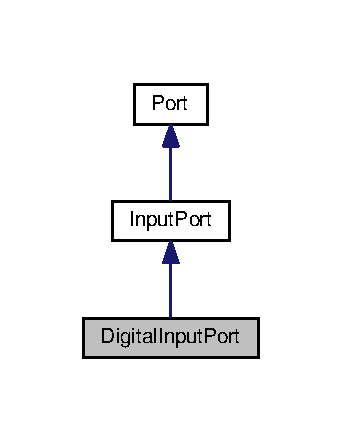
\includegraphics[width=164pt]{classDigitalInputPort__inherit__graph}
\end{center}
\end{figure}


Collaboration diagram for Digital\+Input\+Port\+:\nopagebreak
\begin{figure}[H]
\begin{center}
\leavevmode
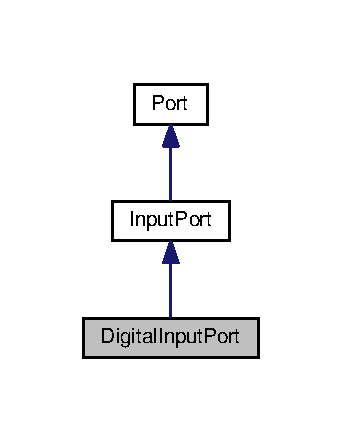
\includegraphics[width=164pt]{classDigitalInputPort__coll__graph}
\end{center}
\end{figure}
\subsection*{Public Member Functions}
\begin{DoxyCompactItemize}
\item 
double \hyperlink{classDigitalInputPort_aada74a73fe70ea59db9399e39190aa5a}{read} ()
\item 
\hyperlink{classDigitalInputPort_a2b7a037e9ea31590c61165f218bd4613}{Digital\+Input\+Port} (unsigned int pin)
\item 
virtual \hyperlink{classDigitalInputPort_aea41ac9de9c02f36efcbf6ec38e1df14}{$\sim$\+Digital\+Input\+Port} ()
\end{DoxyCompactItemize}
\subsection*{Additional Inherited Members}


\subsection{Constructor \& Destructor Documentation}
\index{Digital\+Input\+Port@{Digital\+Input\+Port}!Digital\+Input\+Port@{Digital\+Input\+Port}}
\index{Digital\+Input\+Port@{Digital\+Input\+Port}!Digital\+Input\+Port@{Digital\+Input\+Port}}
\subsubsection[{\texorpdfstring{Digital\+Input\+Port(unsigned int pin)}{DigitalInputPort(unsigned int pin)}}]{\setlength{\rightskip}{0pt plus 5cm}Digital\+Input\+Port\+::\+Digital\+Input\+Port (
\begin{DoxyParamCaption}
\item[{unsigned int}]{pin}
\end{DoxyParamCaption}
)}\hypertarget{classDigitalInputPort_a2b7a037e9ea31590c61165f218bd4613}{}\label{classDigitalInputPort_a2b7a037e9ea31590c61165f218bd4613}
\index{Digital\+Input\+Port@{Digital\+Input\+Port}!````~Digital\+Input\+Port@{$\sim$\+Digital\+Input\+Port}}
\index{````~Digital\+Input\+Port@{$\sim$\+Digital\+Input\+Port}!Digital\+Input\+Port@{Digital\+Input\+Port}}
\subsubsection[{\texorpdfstring{$\sim$\+Digital\+Input\+Port()}{~DigitalInputPort()}}]{\setlength{\rightskip}{0pt plus 5cm}Digital\+Input\+Port\+::$\sim$\+Digital\+Input\+Port (
\begin{DoxyParamCaption}
{}
\end{DoxyParamCaption}
)\hspace{0.3cm}{\ttfamily [virtual]}}\hypertarget{classDigitalInputPort_aea41ac9de9c02f36efcbf6ec38e1df14}{}\label{classDigitalInputPort_aea41ac9de9c02f36efcbf6ec38e1df14}


\subsection{Member Function Documentation}
\index{Digital\+Input\+Port@{Digital\+Input\+Port}!read@{read}}
\index{read@{read}!Digital\+Input\+Port@{Digital\+Input\+Port}}
\subsubsection[{\texorpdfstring{read()}{read()}}]{\setlength{\rightskip}{0pt plus 5cm}double Digital\+Input\+Port\+::read (
\begin{DoxyParamCaption}
{}
\end{DoxyParamCaption}
)\hspace{0.3cm}{\ttfamily [virtual]}}\hypertarget{classDigitalInputPort_aada74a73fe70ea59db9399e39190aa5a}{}\label{classDigitalInputPort_aada74a73fe70ea59db9399e39190aa5a}


Implements \hyperlink{classInputPort_a0dd029736ef41eaf5c1b079c3b8d4ba3}{Input\+Port}.



The documentation for this class was generated from the following files\+:\begin{DoxyCompactItemize}
\item 
\hyperlink{Port_8hpp}{Port.\+hpp}\item 
\hyperlink{Port_8cpp}{Port.\+cpp}\end{DoxyCompactItemize}

\hypertarget{classDigitalOutputPort}{}\section{Digital\+Output\+Port Class Reference}
\label{classDigitalOutputPort}\index{Digital\+Output\+Port@{Digital\+Output\+Port}}


{\ttfamily \#include $<$Port.\+hpp$>$}



Inheritance diagram for Digital\+Output\+Port\+:\nopagebreak
\begin{figure}[H]
\begin{center}
\leavevmode
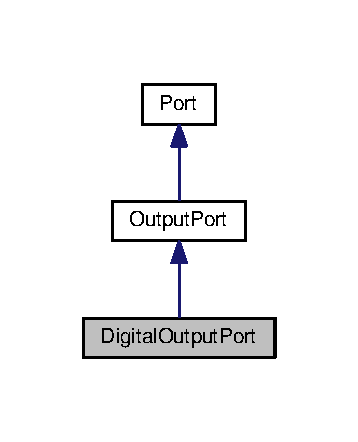
\includegraphics[width=172pt]{classDigitalOutputPort__inherit__graph}
\end{center}
\end{figure}


Collaboration diagram for Digital\+Output\+Port\+:\nopagebreak
\begin{figure}[H]
\begin{center}
\leavevmode
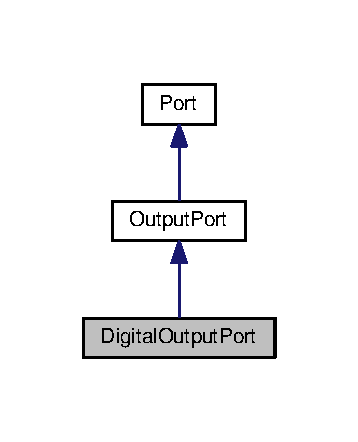
\includegraphics[width=172pt]{classDigitalOutputPort__coll__graph}
\end{center}
\end{figure}
\subsection*{Public Member Functions}
\begin{DoxyCompactItemize}
\item 
void \hyperlink{classDigitalOutputPort_a822b172983a6c03f83ea87215d3dac18}{write} (double value)
\item 
\hyperlink{classDigitalOutputPort_a05ea9b4e8690a0a87d0ea4775cd799c8}{Digital\+Output\+Port} (unsigned int pin)
\item 
virtual \hyperlink{classDigitalOutputPort_aa38e2275592940e5d7e833569af17d2f}{$\sim$\+Digital\+Output\+Port} ()
\end{DoxyCompactItemize}
\subsection*{Additional Inherited Members}


\subsection{Constructor \& Destructor Documentation}
\index{Digital\+Output\+Port@{Digital\+Output\+Port}!Digital\+Output\+Port@{Digital\+Output\+Port}}
\index{Digital\+Output\+Port@{Digital\+Output\+Port}!Digital\+Output\+Port@{Digital\+Output\+Port}}
\subsubsection[{\texorpdfstring{Digital\+Output\+Port(unsigned int pin)}{DigitalOutputPort(unsigned int pin)}}]{\setlength{\rightskip}{0pt plus 5cm}Digital\+Output\+Port\+::\+Digital\+Output\+Port (
\begin{DoxyParamCaption}
\item[{unsigned int}]{pin}
\end{DoxyParamCaption}
)}\hypertarget{classDigitalOutputPort_a05ea9b4e8690a0a87d0ea4775cd799c8}{}\label{classDigitalOutputPort_a05ea9b4e8690a0a87d0ea4775cd799c8}
\index{Digital\+Output\+Port@{Digital\+Output\+Port}!````~Digital\+Output\+Port@{$\sim$\+Digital\+Output\+Port}}
\index{````~Digital\+Output\+Port@{$\sim$\+Digital\+Output\+Port}!Digital\+Output\+Port@{Digital\+Output\+Port}}
\subsubsection[{\texorpdfstring{$\sim$\+Digital\+Output\+Port()}{~DigitalOutputPort()}}]{\setlength{\rightskip}{0pt plus 5cm}Digital\+Output\+Port\+::$\sim$\+Digital\+Output\+Port (
\begin{DoxyParamCaption}
{}
\end{DoxyParamCaption}
)\hspace{0.3cm}{\ttfamily [virtual]}}\hypertarget{classDigitalOutputPort_aa38e2275592940e5d7e833569af17d2f}{}\label{classDigitalOutputPort_aa38e2275592940e5d7e833569af17d2f}


\subsection{Member Function Documentation}
\index{Digital\+Output\+Port@{Digital\+Output\+Port}!write@{write}}
\index{write@{write}!Digital\+Output\+Port@{Digital\+Output\+Port}}
\subsubsection[{\texorpdfstring{write(double value)}{write(double value)}}]{\setlength{\rightskip}{0pt plus 5cm}void Digital\+Output\+Port\+::write (
\begin{DoxyParamCaption}
\item[{double}]{value}
\end{DoxyParamCaption}
)\hspace{0.3cm}{\ttfamily [virtual]}}\hypertarget{classDigitalOutputPort_a822b172983a6c03f83ea87215d3dac18}{}\label{classDigitalOutputPort_a822b172983a6c03f83ea87215d3dac18}


Implements \hyperlink{classOutputPort_a36ab0474c09692287507ddb783671566}{Output\+Port}.



The documentation for this class was generated from the following files\+:\begin{DoxyCompactItemize}
\item 
\hyperlink{Port_8hpp}{Port.\+hpp}\item 
\hyperlink{Port_8cpp}{Port.\+cpp}\end{DoxyCompactItemize}

\hypertarget{classEndTrialCommand}{}\section{End\+Trial\+Command Class Reference}
\label{classEndTrialCommand}\index{End\+Trial\+Command@{End\+Trial\+Command}}


{\ttfamily \#include $<$Commands.\+hpp$>$}



Inheritance diagram for End\+Trial\+Command\+:\nopagebreak
\begin{figure}[H]
\begin{center}
\leavevmode
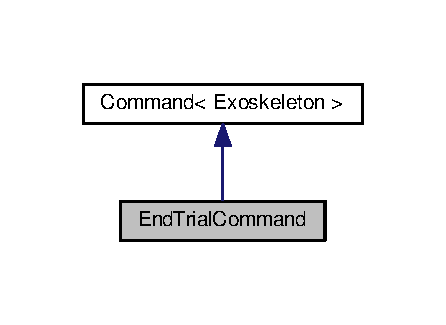
\includegraphics[width=214pt]{classEndTrialCommand__inherit__graph}
\end{center}
\end{figure}


Collaboration diagram for End\+Trial\+Command\+:\nopagebreak
\begin{figure}[H]
\begin{center}
\leavevmode
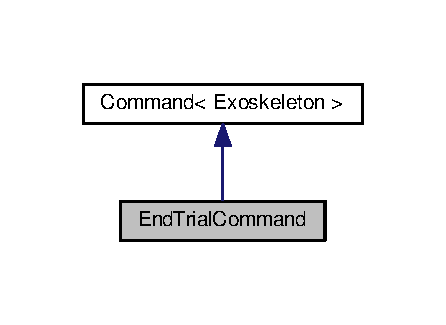
\includegraphics[width=214pt]{classEndTrialCommand__coll__graph}
\end{center}
\end{figure}
\subsection*{Public Member Functions}
\begin{DoxyCompactItemize}
\item 
virtual void \hyperlink{classEndTrialCommand_ac07f0eddff9b21da6cb302489aac19c7}{execute} (\hyperlink{classExoskeleton}{Exoskeleton} $\ast$exo)
\end{DoxyCompactItemize}


\subsection{Member Function Documentation}
\index{End\+Trial\+Command@{End\+Trial\+Command}!execute@{execute}}
\index{execute@{execute}!End\+Trial\+Command@{End\+Trial\+Command}}
\subsubsection[{\texorpdfstring{execute(\+Exoskeleton $\ast$exo)}{execute(Exoskeleton *exo)}}]{\setlength{\rightskip}{0pt plus 5cm}void End\+Trial\+Command\+::execute (
\begin{DoxyParamCaption}
\item[{{\bf Exoskeleton} $\ast$}]{exo}
\end{DoxyParamCaption}
)\hspace{0.3cm}{\ttfamily [virtual]}}\hypertarget{classEndTrialCommand_ac07f0eddff9b21da6cb302489aac19c7}{}\label{classEndTrialCommand_ac07f0eddff9b21da6cb302489aac19c7}


Implements \hyperlink{classCommand_af8fc41633b1d53b23da6a99c81c0689c}{Command$<$ Exoskeleton $>$}.



The documentation for this class was generated from the following files\+:\begin{DoxyCompactItemize}
\item 
\hyperlink{Commands_8hpp}{Commands.\+hpp}\item 
\hyperlink{Commands_8cpp}{Commands.\+cpp}\end{DoxyCompactItemize}

\hypertarget{classEndTrialTransmission}{}\section{End\+Trial\+Transmission Class Reference}
\label{classEndTrialTransmission}\index{End\+Trial\+Transmission@{End\+Trial\+Transmission}}


{\ttfamily \#include $<$Transmission.\+hpp$>$}



Inheritance diagram for End\+Trial\+Transmission\+:\nopagebreak
\begin{figure}[H]
\begin{center}
\leavevmode
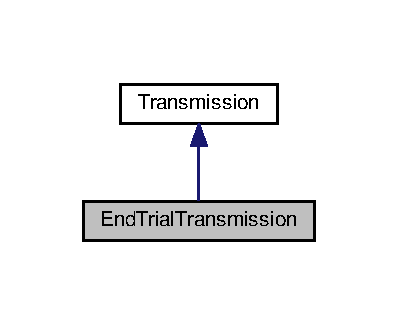
\includegraphics[width=191pt]{classEndTrialTransmission__inherit__graph}
\end{center}
\end{figure}


Collaboration diagram for End\+Trial\+Transmission\+:\nopagebreak
\begin{figure}[H]
\begin{center}
\leavevmode
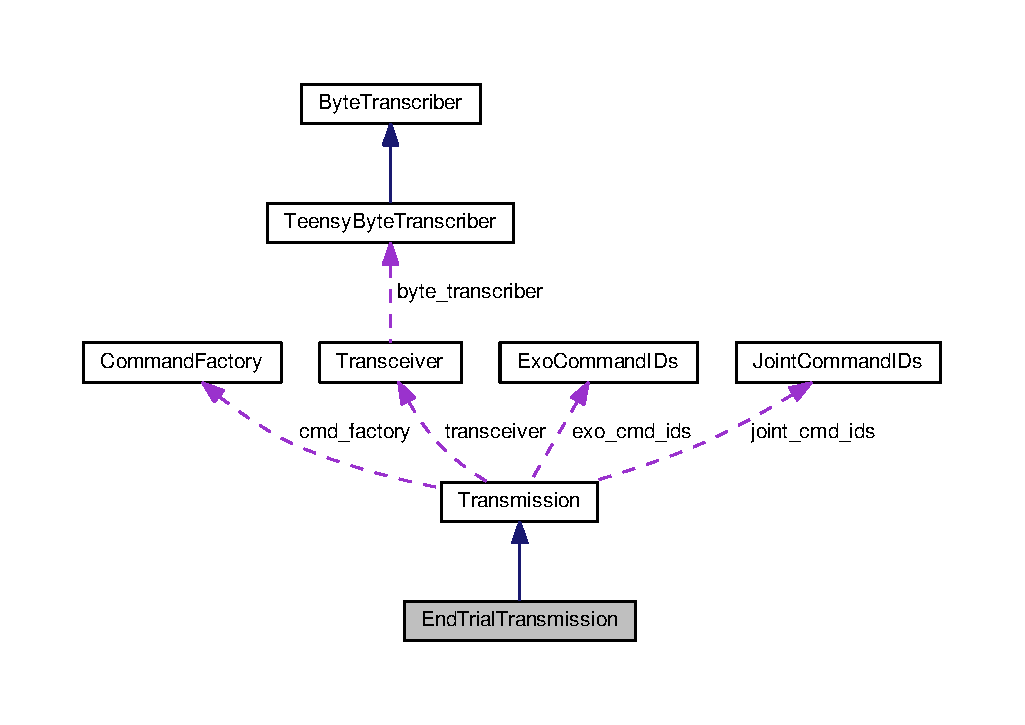
\includegraphics[width=350pt]{classEndTrialTransmission__coll__graph}
\end{center}
\end{figure}
\subsection*{Public Member Functions}
\begin{DoxyCompactItemize}
\item 
\hyperlink{classEndTrialTransmission_a300f0b5c7535f8979dbe25a6012b46b5}{End\+Trial\+Transmission} (\hyperlink{classTransceiver}{Transceiver} $\ast$\hyperlink{classTransmission_a4136f9d979a928565232a2d3d6eb5ac5}{transceiver}, \hyperlink{classCommandFactory}{Command\+Factory} $\ast$cmd)
\end{DoxyCompactItemize}
\subsection*{Additional Inherited Members}


\subsection{Constructor \& Destructor Documentation}
\index{End\+Trial\+Transmission@{End\+Trial\+Transmission}!End\+Trial\+Transmission@{End\+Trial\+Transmission}}
\index{End\+Trial\+Transmission@{End\+Trial\+Transmission}!End\+Trial\+Transmission@{End\+Trial\+Transmission}}
\subsubsection[{\texorpdfstring{End\+Trial\+Transmission(\+Transceiver $\ast$transceiver, Command\+Factory $\ast$cmd)}{EndTrialTransmission(Transceiver *transceiver, CommandFactory *cmd)}}]{\setlength{\rightskip}{0pt plus 5cm}End\+Trial\+Transmission\+::\+End\+Trial\+Transmission (
\begin{DoxyParamCaption}
\item[{{\bf Transceiver} $\ast$}]{transceiver, }
\item[{{\bf Command\+Factory} $\ast$}]{cmd}
\end{DoxyParamCaption}
)\hspace{0.3cm}{\ttfamily [explicit]}}\hypertarget{classEndTrialTransmission_a300f0b5c7535f8979dbe25a6012b46b5}{}\label{classEndTrialTransmission_a300f0b5c7535f8979dbe25a6012b46b5}


The documentation for this class was generated from the following files\+:\begin{DoxyCompactItemize}
\item 
\hyperlink{Transmission_8hpp}{Transmission.\+hpp}\item 
\hyperlink{Transmission_8cpp}{Transmission.\+cpp}\end{DoxyCompactItemize}

\hypertarget{classExoBuilder}{}\section{Exo\+Builder Class Reference}
\label{classExoBuilder}\index{Exo\+Builder@{Exo\+Builder}}


{\ttfamily \#include $<$Exo\+Builder.\+hpp$>$}

\subsection*{Public Member Functions}
\begin{DoxyCompactItemize}
\item 
\hyperlink{classExoBuilder_a78731930b38367f2ed6a1d07fd4c170e}{$\sim$\+Exo\+Builder} ()
\item 
\hyperlink{classExoBuilder}{Exo\+Builder} $\ast$ \hyperlink{classExoBuilder_a0dd286bd1f02733240264f64622e3893}{add\+Transceiver} (\hyperlink{classTxPort}{Tx\+Port} $\ast$tx, \hyperlink{classRxPort}{Rx\+Port} $\ast$rx)
\item 
\hyperlink{classExoBuilder}{Exo\+Builder} $\ast$ \hyperlink{classExoBuilder_a6e4815a31b8b4b7bed3c4daac323d52e}{add\+Motor\+Enable} (\hyperlink{classOutputPort}{Output\+Port} $\ast$motor\+\_\+enable\+\_\+port)
\item 
\hyperlink{classExoBuilder}{Exo\+Builder} $\ast$ \hyperlink{classExoBuilder_a70dddb8a338cb907d4b36f7e0aad2de1}{add\+Led\+Port} (\hyperlink{classOutputPort}{Output\+Port} $\ast$led\+\_\+port)
\item 
\hyperlink{classLegBuilder}{Leg\+Builder} $\ast$ \hyperlink{classExoBuilder_a934166b17a4be037b9aa6fcce9295c05}{begin\+Right\+Leg} ()
\item 
\hyperlink{classLegBuilder}{Leg\+Builder} $\ast$ \hyperlink{classExoBuilder_a96c398cb523b039319dba0461e30ac79}{begin\+Left\+Leg} ()
\item 
\hyperlink{classExoskeleton}{Exoskeleton} $\ast$ \hyperlink{classExoBuilder_ae121300fd8a1d4f1d8b10093c031d9e2}{build} ()
\end{DoxyCompactItemize}


\subsection{Constructor \& Destructor Documentation}
\index{Exo\+Builder@{Exo\+Builder}!````~Exo\+Builder@{$\sim$\+Exo\+Builder}}
\index{````~Exo\+Builder@{$\sim$\+Exo\+Builder}!Exo\+Builder@{Exo\+Builder}}
\subsubsection[{\texorpdfstring{$\sim$\+Exo\+Builder()}{~ExoBuilder()}}]{\setlength{\rightskip}{0pt plus 5cm}Exo\+Builder\+::$\sim$\+Exo\+Builder (
\begin{DoxyParamCaption}
{}
\end{DoxyParamCaption}
)}\hypertarget{classExoBuilder_a78731930b38367f2ed6a1d07fd4c170e}{}\label{classExoBuilder_a78731930b38367f2ed6a1d07fd4c170e}


\subsection{Member Function Documentation}
\index{Exo\+Builder@{Exo\+Builder}!add\+Led\+Port@{add\+Led\+Port}}
\index{add\+Led\+Port@{add\+Led\+Port}!Exo\+Builder@{Exo\+Builder}}
\subsubsection[{\texorpdfstring{add\+Led\+Port(\+Output\+Port $\ast$led\+\_\+port)}{addLedPort(OutputPort *led_port)}}]{\setlength{\rightskip}{0pt plus 5cm}{\bf Exo\+Builder} $\ast$ Exo\+Builder\+::add\+Led\+Port (
\begin{DoxyParamCaption}
\item[{{\bf Output\+Port} $\ast$}]{led\+\_\+port}
\end{DoxyParamCaption}
)}\hypertarget{classExoBuilder_a70dddb8a338cb907d4b36f7e0aad2de1}{}\label{classExoBuilder_a70dddb8a338cb907d4b36f7e0aad2de1}
\index{Exo\+Builder@{Exo\+Builder}!add\+Motor\+Enable@{add\+Motor\+Enable}}
\index{add\+Motor\+Enable@{add\+Motor\+Enable}!Exo\+Builder@{Exo\+Builder}}
\subsubsection[{\texorpdfstring{add\+Motor\+Enable(\+Output\+Port $\ast$motor\+\_\+enable\+\_\+port)}{addMotorEnable(OutputPort *motor_enable_port)}}]{\setlength{\rightskip}{0pt plus 5cm}{\bf Exo\+Builder} $\ast$ Exo\+Builder\+::add\+Motor\+Enable (
\begin{DoxyParamCaption}
\item[{{\bf Output\+Port} $\ast$}]{motor\+\_\+enable\+\_\+port}
\end{DoxyParamCaption}
)}\hypertarget{classExoBuilder_a6e4815a31b8b4b7bed3c4daac323d52e}{}\label{classExoBuilder_a6e4815a31b8b4b7bed3c4daac323d52e}
\index{Exo\+Builder@{Exo\+Builder}!add\+Transceiver@{add\+Transceiver}}
\index{add\+Transceiver@{add\+Transceiver}!Exo\+Builder@{Exo\+Builder}}
\subsubsection[{\texorpdfstring{add\+Transceiver(\+Tx\+Port $\ast$tx, Rx\+Port $\ast$rx)}{addTransceiver(TxPort *tx, RxPort *rx)}}]{\setlength{\rightskip}{0pt plus 5cm}{\bf Exo\+Builder} $\ast$ Exo\+Builder\+::add\+Transceiver (
\begin{DoxyParamCaption}
\item[{{\bf Tx\+Port} $\ast$}]{tx, }
\item[{{\bf Rx\+Port} $\ast$}]{rx}
\end{DoxyParamCaption}
)}\hypertarget{classExoBuilder_a0dd286bd1f02733240264f64622e3893}{}\label{classExoBuilder_a0dd286bd1f02733240264f64622e3893}
\index{Exo\+Builder@{Exo\+Builder}!begin\+Left\+Leg@{begin\+Left\+Leg}}
\index{begin\+Left\+Leg@{begin\+Left\+Leg}!Exo\+Builder@{Exo\+Builder}}
\subsubsection[{\texorpdfstring{begin\+Left\+Leg()}{beginLeftLeg()}}]{\setlength{\rightskip}{0pt plus 5cm}{\bf Leg\+Builder} $\ast$ Exo\+Builder\+::begin\+Left\+Leg (
\begin{DoxyParamCaption}
{}
\end{DoxyParamCaption}
)}\hypertarget{classExoBuilder_a96c398cb523b039319dba0461e30ac79}{}\label{classExoBuilder_a96c398cb523b039319dba0461e30ac79}
\index{Exo\+Builder@{Exo\+Builder}!begin\+Right\+Leg@{begin\+Right\+Leg}}
\index{begin\+Right\+Leg@{begin\+Right\+Leg}!Exo\+Builder@{Exo\+Builder}}
\subsubsection[{\texorpdfstring{begin\+Right\+Leg()}{beginRightLeg()}}]{\setlength{\rightskip}{0pt plus 5cm}{\bf Leg\+Builder} $\ast$ Exo\+Builder\+::begin\+Right\+Leg (
\begin{DoxyParamCaption}
{}
\end{DoxyParamCaption}
)}\hypertarget{classExoBuilder_a934166b17a4be037b9aa6fcce9295c05}{}\label{classExoBuilder_a934166b17a4be037b9aa6fcce9295c05}
\index{Exo\+Builder@{Exo\+Builder}!build@{build}}
\index{build@{build}!Exo\+Builder@{Exo\+Builder}}
\subsubsection[{\texorpdfstring{build()}{build()}}]{\setlength{\rightskip}{0pt plus 5cm}{\bf Exoskeleton} $\ast$ Exo\+Builder\+::build (
\begin{DoxyParamCaption}
{}
\end{DoxyParamCaption}
)}\hypertarget{classExoBuilder_ae121300fd8a1d4f1d8b10093c031d9e2}{}\label{classExoBuilder_ae121300fd8a1d4f1d8b10093c031d9e2}


The documentation for this class was generated from the following files\+:\begin{DoxyCompactItemize}
\item 
\hyperlink{ExoBuilder_8hpp}{Exo\+Builder.\+hpp}\item 
\hyperlink{ExoBuilder_8cpp}{Exo\+Builder.\+cpp}\end{DoxyCompactItemize}

\hypertarget{classExoCommandIDs}{}\section{Exo\+Command\+I\+Ds Class Reference}
\label{classExoCommandIDs}\index{Exo\+Command\+I\+Ds@{Exo\+Command\+I\+Ds}}


{\ttfamily \#include $<$Commands.\+hpp$>$}

\subsection*{Static Public Attributes}
\begin{DoxyCompactItemize}
\item 
static const \hyperlink{Commands_8hpp_a4a0419b573bf683fef9162331e6ec74e}{Exo\+Command\+ID} \hyperlink{classExoCommandIDs_afb527e21397c4ed34c37761c8e66c3a8}{S\+T\+A\+R\+T\+\_\+\+T\+R\+I\+AL} = 0
\item 
static const \hyperlink{Commands_8hpp_a4a0419b573bf683fef9162331e6ec74e}{Exo\+Command\+ID} \hyperlink{classExoCommandIDs_a72245f17b9ebda2742d181facde3c192}{E\+N\+D\+\_\+\+T\+R\+I\+AL} = 1
\item 
static const \hyperlink{Commands_8hpp_a4a0419b573bf683fef9162331e6ec74e}{Exo\+Command\+ID} \hyperlink{classExoCommandIDs_af8e8a8a8a8e1bf4ebb8ad2ef561f8dd9}{C\+A\+L\+I\+B\+R\+A\+T\+E\+\_\+\+T\+O\+R\+Q\+UE} = 2
\item 
static const \hyperlink{Commands_8hpp_a4a0419b573bf683fef9162331e6ec74e}{Exo\+Command\+ID} \hyperlink{classExoCommandIDs_ae709797110384e57f92e391ae7ffa5dc}{C\+A\+L\+I\+B\+R\+A\+T\+E\+\_\+\+F\+S\+RS} = 3
\end{DoxyCompactItemize}


\subsection{Member Data Documentation}
\index{Exo\+Command\+I\+Ds@{Exo\+Command\+I\+Ds}!C\+A\+L\+I\+B\+R\+A\+T\+E\+\_\+\+F\+S\+RS@{C\+A\+L\+I\+B\+R\+A\+T\+E\+\_\+\+F\+S\+RS}}
\index{C\+A\+L\+I\+B\+R\+A\+T\+E\+\_\+\+F\+S\+RS@{C\+A\+L\+I\+B\+R\+A\+T\+E\+\_\+\+F\+S\+RS}!Exo\+Command\+I\+Ds@{Exo\+Command\+I\+Ds}}
\subsubsection[{\texorpdfstring{C\+A\+L\+I\+B\+R\+A\+T\+E\+\_\+\+F\+S\+RS}{CALIBRATE_FSRS}}]{\setlength{\rightskip}{0pt plus 5cm}const {\bf Exo\+Command\+ID} Exo\+Command\+I\+Ds\+::\+C\+A\+L\+I\+B\+R\+A\+T\+E\+\_\+\+F\+S\+RS = 3\hspace{0.3cm}{\ttfamily [static]}}\hypertarget{classExoCommandIDs_ae709797110384e57f92e391ae7ffa5dc}{}\label{classExoCommandIDs_ae709797110384e57f92e391ae7ffa5dc}
\index{Exo\+Command\+I\+Ds@{Exo\+Command\+I\+Ds}!C\+A\+L\+I\+B\+R\+A\+T\+E\+\_\+\+T\+O\+R\+Q\+UE@{C\+A\+L\+I\+B\+R\+A\+T\+E\+\_\+\+T\+O\+R\+Q\+UE}}
\index{C\+A\+L\+I\+B\+R\+A\+T\+E\+\_\+\+T\+O\+R\+Q\+UE@{C\+A\+L\+I\+B\+R\+A\+T\+E\+\_\+\+T\+O\+R\+Q\+UE}!Exo\+Command\+I\+Ds@{Exo\+Command\+I\+Ds}}
\subsubsection[{\texorpdfstring{C\+A\+L\+I\+B\+R\+A\+T\+E\+\_\+\+T\+O\+R\+Q\+UE}{CALIBRATE_TORQUE}}]{\setlength{\rightskip}{0pt plus 5cm}const {\bf Exo\+Command\+ID} Exo\+Command\+I\+Ds\+::\+C\+A\+L\+I\+B\+R\+A\+T\+E\+\_\+\+T\+O\+R\+Q\+UE = 2\hspace{0.3cm}{\ttfamily [static]}}\hypertarget{classExoCommandIDs_af8e8a8a8a8e1bf4ebb8ad2ef561f8dd9}{}\label{classExoCommandIDs_af8e8a8a8a8e1bf4ebb8ad2ef561f8dd9}
\index{Exo\+Command\+I\+Ds@{Exo\+Command\+I\+Ds}!E\+N\+D\+\_\+\+T\+R\+I\+AL@{E\+N\+D\+\_\+\+T\+R\+I\+AL}}
\index{E\+N\+D\+\_\+\+T\+R\+I\+AL@{E\+N\+D\+\_\+\+T\+R\+I\+AL}!Exo\+Command\+I\+Ds@{Exo\+Command\+I\+Ds}}
\subsubsection[{\texorpdfstring{E\+N\+D\+\_\+\+T\+R\+I\+AL}{END_TRIAL}}]{\setlength{\rightskip}{0pt plus 5cm}const {\bf Exo\+Command\+ID} Exo\+Command\+I\+Ds\+::\+E\+N\+D\+\_\+\+T\+R\+I\+AL = 1\hspace{0.3cm}{\ttfamily [static]}}\hypertarget{classExoCommandIDs_a72245f17b9ebda2742d181facde3c192}{}\label{classExoCommandIDs_a72245f17b9ebda2742d181facde3c192}
\index{Exo\+Command\+I\+Ds@{Exo\+Command\+I\+Ds}!S\+T\+A\+R\+T\+\_\+\+T\+R\+I\+AL@{S\+T\+A\+R\+T\+\_\+\+T\+R\+I\+AL}}
\index{S\+T\+A\+R\+T\+\_\+\+T\+R\+I\+AL@{S\+T\+A\+R\+T\+\_\+\+T\+R\+I\+AL}!Exo\+Command\+I\+Ds@{Exo\+Command\+I\+Ds}}
\subsubsection[{\texorpdfstring{S\+T\+A\+R\+T\+\_\+\+T\+R\+I\+AL}{START_TRIAL}}]{\setlength{\rightskip}{0pt plus 5cm}const {\bf Exo\+Command\+ID} Exo\+Command\+I\+Ds\+::\+S\+T\+A\+R\+T\+\_\+\+T\+R\+I\+AL = 0\hspace{0.3cm}{\ttfamily [static]}}\hypertarget{classExoCommandIDs_afb527e21397c4ed34c37761c8e66c3a8}{}\label{classExoCommandIDs_afb527e21397c4ed34c37761c8e66c3a8}


The documentation for this class was generated from the following file\+:\begin{DoxyCompactItemize}
\item 
\hyperlink{Commands_8hpp}{Commands.\+hpp}\end{DoxyCompactItemize}

\hypertarget{classExoDirector}{}\section{Exo\+Director Class Reference}
\label{classExoDirector}\index{Exo\+Director@{Exo\+Director}}


{\ttfamily \#include $<$Exo\+Builder.\+hpp$>$}



Inheritance diagram for Exo\+Director\+:\nopagebreak
\begin{figure}[H]
\begin{center}
\leavevmode
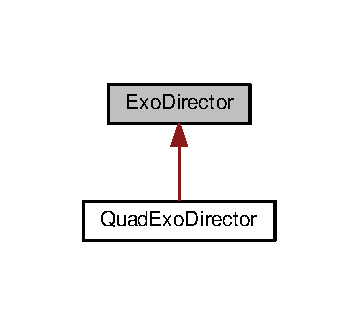
\includegraphics[width=172pt]{classExoDirector__inherit__graph}
\end{center}
\end{figure}
\subsection*{Public Member Functions}
\begin{DoxyCompactItemize}
\item 
virtual \hyperlink{classExoskeleton}{Exoskeleton} $\ast$ \hyperlink{classExoDirector_a47e0aaa6573aee9bfd3cc3d24634adee}{build} (\hyperlink{classBoard}{Board} $\ast$board)=0
\end{DoxyCompactItemize}


\subsection{Member Function Documentation}
\index{Exo\+Director@{Exo\+Director}!build@{build}}
\index{build@{build}!Exo\+Director@{Exo\+Director}}
\subsubsection[{\texorpdfstring{build(\+Board $\ast$board)=0}{build(Board *board)=0}}]{\setlength{\rightskip}{0pt plus 5cm}virtual {\bf Exoskeleton}$\ast$ Exo\+Director\+::build (
\begin{DoxyParamCaption}
\item[{{\bf Board} $\ast$}]{board}
\end{DoxyParamCaption}
)\hspace{0.3cm}{\ttfamily [pure virtual]}}\hypertarget{classExoDirector_a47e0aaa6573aee9bfd3cc3d24634adee}{}\label{classExoDirector_a47e0aaa6573aee9bfd3cc3d24634adee}


Implemented in \hyperlink{classQuadExoDirector_a84ad89c3c1c005ccb40c4b9a91c5e773}{Quad\+Exo\+Director}.



The documentation for this class was generated from the following file\+:\begin{DoxyCompactItemize}
\item 
\hyperlink{ExoBuilder_8hpp}{Exo\+Builder.\+hpp}\end{DoxyCompactItemize}

\hypertarget{classExoMessage}{}\section{Exo\+Message Class Reference}
\label{classExoMessage}\index{Exo\+Message@{Exo\+Message}}


{\ttfamily \#include $<$Message.\+hpp$>$}



Inheritance diagram for Exo\+Message\+:\nopagebreak
\begin{figure}[H]
\begin{center}
\leavevmode
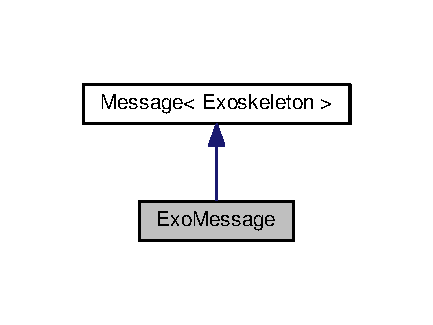
\includegraphics[width=208pt]{classExoMessage__inherit__graph}
\end{center}
\end{figure}


Collaboration diagram for Exo\+Message\+:
\nopagebreak
\begin{figure}[H]
\begin{center}
\leavevmode
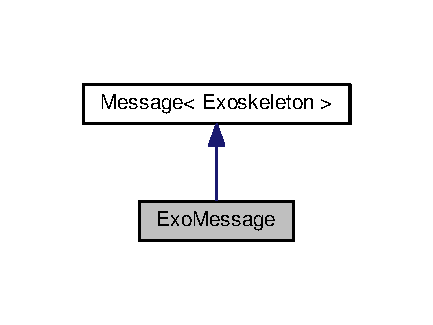
\includegraphics[width=208pt]{classExoMessage__coll__graph}
\end{center}
\end{figure}
\subsection*{Public Member Functions}
\begin{DoxyCompactItemize}
\item 
\hyperlink{classExoMessage_a0ce38c72897da367a035daf85574b78b}{Exo\+Message} (\hyperlink{classLinkedList}{Linked\+List}$<$ \hyperlink{classCommand}{Command}$<$ \hyperlink{classExoskeleton}{Exoskeleton} $>$ $\ast$ $>$ $\ast$pre\+\_\+commands, \hyperlink{classLinkedList}{Linked\+List}$<$ \hyperlink{classCommand}{Command}$<$ \hyperlink{classExoskeleton}{Exoskeleton} $>$ $\ast$ $>$ $\ast$post\+\_\+commands, \hyperlink{classLegMessage}{Leg\+Message} $\ast$right\+\_\+leg\+\_\+msg, \hyperlink{classLegMessage}{Leg\+Message} $\ast$left\+\_\+leg\+\_\+msg)
\item 
\hyperlink{classExoMessage_a79fc89994766ad128dd7857eacaabfea}{$\sim$\+Exo\+Message} ()
\item 
void \hyperlink{classExoMessage_a9bd51f224fcb2cb3749d6eda6df53299}{message\+Area} (\hyperlink{JointSelect_8hpp_a0b0b6279ef5d4a446f8f07404dc868d3}{Area\+ID} id)
\item 
void \hyperlink{classExoMessage_ab2bbb8222325944e6bae4ca75d00175a}{message\+Right\+Leg} (\hyperlink{classLeg}{Leg} $\ast$right)
\item 
void \hyperlink{classExoMessage_ac1555c53ca0d1c3b953cc343b7ca47d4}{message\+Left\+Leg} (\hyperlink{classLeg}{Leg} $\ast$left)
\end{DoxyCompactItemize}


\subsection{Constructor \& Destructor Documentation}
\index{Exo\+Message@{Exo\+Message}!Exo\+Message@{Exo\+Message}}
\index{Exo\+Message@{Exo\+Message}!Exo\+Message@{Exo\+Message}}
\subsubsection[{\texorpdfstring{Exo\+Message(\+Linked\+List$<$ Command$<$ Exoskeleton $>$ $\ast$ $>$ $\ast$pre\+\_\+commands, Linked\+List$<$ Command$<$ Exoskeleton $>$ $\ast$ $>$ $\ast$post\+\_\+commands, Leg\+Message $\ast$right\+\_\+leg\+\_\+msg, Leg\+Message $\ast$left\+\_\+leg\+\_\+msg)}{ExoMessage(LinkedList< Command< Exoskeleton > * > *pre_commands, LinkedList< Command< Exoskeleton > * > *post_commands, LegMessage *right_leg_msg, LegMessage *left_leg_msg)}}]{\setlength{\rightskip}{0pt plus 5cm}Exo\+Message\+::\+Exo\+Message (
\begin{DoxyParamCaption}
\item[{{\bf Linked\+List}$<$ {\bf Command}$<$ {\bf Exoskeleton} $>$ $\ast$ $>$ $\ast$}]{pre\+\_\+commands, }
\item[{{\bf Linked\+List}$<$ {\bf Command}$<$ {\bf Exoskeleton} $>$ $\ast$ $>$ $\ast$}]{post\+\_\+commands, }
\item[{{\bf Leg\+Message} $\ast$}]{right\+\_\+leg\+\_\+msg, }
\item[{{\bf Leg\+Message} $\ast$}]{left\+\_\+leg\+\_\+msg}
\end{DoxyParamCaption}
)}\hypertarget{classExoMessage_a0ce38c72897da367a035daf85574b78b}{}\label{classExoMessage_a0ce38c72897da367a035daf85574b78b}
\index{Exo\+Message@{Exo\+Message}!````~Exo\+Message@{$\sim$\+Exo\+Message}}
\index{````~Exo\+Message@{$\sim$\+Exo\+Message}!Exo\+Message@{Exo\+Message}}
\subsubsection[{\texorpdfstring{$\sim$\+Exo\+Message()}{~ExoMessage()}}]{\setlength{\rightskip}{0pt plus 5cm}Exo\+Message\+::$\sim$\+Exo\+Message (
\begin{DoxyParamCaption}
{}
\end{DoxyParamCaption}
)}\hypertarget{classExoMessage_a79fc89994766ad128dd7857eacaabfea}{}\label{classExoMessage_a79fc89994766ad128dd7857eacaabfea}


\subsection{Member Function Documentation}
\index{Exo\+Message@{Exo\+Message}!message\+Area@{message\+Area}}
\index{message\+Area@{message\+Area}!Exo\+Message@{Exo\+Message}}
\subsubsection[{\texorpdfstring{message\+Area(\+Area\+I\+D id)}{messageArea(AreaID id)}}]{\setlength{\rightskip}{0pt plus 5cm}void Exo\+Message\+::message\+Area (
\begin{DoxyParamCaption}
\item[{{\bf Area\+ID}}]{id}
\end{DoxyParamCaption}
)}\hypertarget{classExoMessage_a9bd51f224fcb2cb3749d6eda6df53299}{}\label{classExoMessage_a9bd51f224fcb2cb3749d6eda6df53299}
\index{Exo\+Message@{Exo\+Message}!message\+Left\+Leg@{message\+Left\+Leg}}
\index{message\+Left\+Leg@{message\+Left\+Leg}!Exo\+Message@{Exo\+Message}}
\subsubsection[{\texorpdfstring{message\+Left\+Leg(\+Leg $\ast$left)}{messageLeftLeg(Leg *left)}}]{\setlength{\rightskip}{0pt plus 5cm}void Exo\+Message\+::message\+Left\+Leg (
\begin{DoxyParamCaption}
\item[{{\bf Leg} $\ast$}]{left}
\end{DoxyParamCaption}
)}\hypertarget{classExoMessage_ac1555c53ca0d1c3b953cc343b7ca47d4}{}\label{classExoMessage_ac1555c53ca0d1c3b953cc343b7ca47d4}
\index{Exo\+Message@{Exo\+Message}!message\+Right\+Leg@{message\+Right\+Leg}}
\index{message\+Right\+Leg@{message\+Right\+Leg}!Exo\+Message@{Exo\+Message}}
\subsubsection[{\texorpdfstring{message\+Right\+Leg(\+Leg $\ast$right)}{messageRightLeg(Leg *right)}}]{\setlength{\rightskip}{0pt plus 5cm}void Exo\+Message\+::message\+Right\+Leg (
\begin{DoxyParamCaption}
\item[{{\bf Leg} $\ast$}]{right}
\end{DoxyParamCaption}
)}\hypertarget{classExoMessage_ab2bbb8222325944e6bae4ca75d00175a}{}\label{classExoMessage_ab2bbb8222325944e6bae4ca75d00175a}


The documentation for this class was generated from the following files\+:\begin{DoxyCompactItemize}
\item 
\hyperlink{Message_8hpp}{Message.\+hpp}\item 
\hyperlink{Message_8cpp}{Message.\+cpp}\end{DoxyCompactItemize}

\hypertarget{classExoMessageBuilder}{}\section{Exo\+Message\+Builder Class Reference}
\label{classExoMessageBuilder}\index{Exo\+Message\+Builder@{Exo\+Message\+Builder}}


{\ttfamily \#include $<$Message.\+hpp$>$}



Inheritance diagram for Exo\+Message\+Builder\+:\nopagebreak
\begin{figure}[H]
\begin{center}
\leavevmode
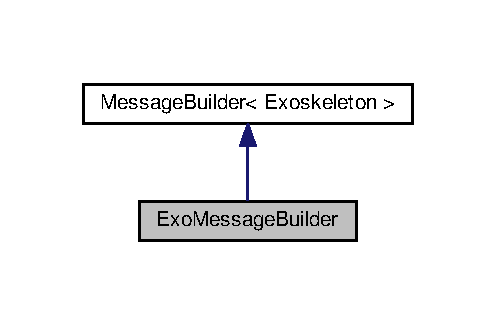
\includegraphics[width=238pt]{classExoMessageBuilder__inherit__graph}
\end{center}
\end{figure}


Collaboration diagram for Exo\+Message\+Builder\+:
\nopagebreak
\begin{figure}[H]
\begin{center}
\leavevmode
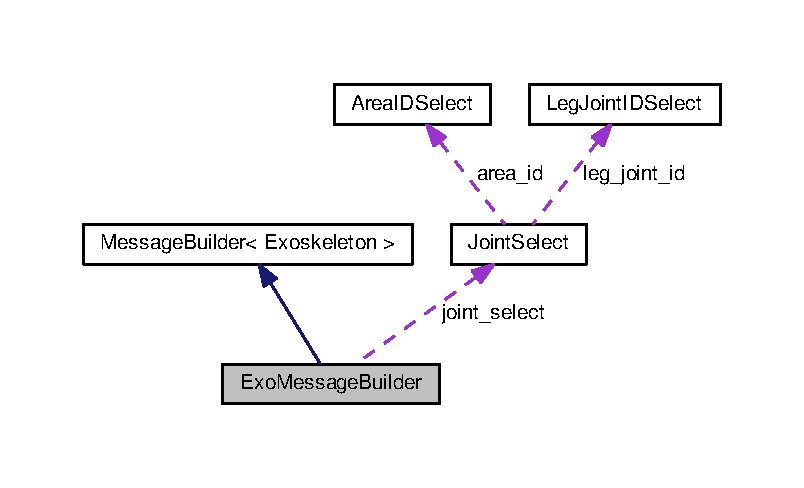
\includegraphics[width=350pt]{classExoMessageBuilder__coll__graph}
\end{center}
\end{figure}
\subsection*{Public Member Functions}
\begin{DoxyCompactItemize}
\item 
\hyperlink{classExoMessageBuilder_a945a7e743d70ad2265be0131d378705b}{Exo\+Message\+Builder} ()
\item 
\hyperlink{classExoMessageBuilder_a42b77a7a914cec1accf35698c653005b}{$\sim$\+Exo\+Message\+Builder} ()
\item 
\hyperlink{classExoMessageBuilder}{Exo\+Message\+Builder} $\ast$ \hyperlink{classExoMessageBuilder_a8628cf50333fa20f8309ff6dbf5bb3c1}{add\+Pre\+Command} (\hyperlink{classCommand}{Command}$<$ \hyperlink{classExoskeleton}{Exoskeleton} $>$ $\ast$command)
\item 
\hyperlink{classExoMessageBuilder}{Exo\+Message\+Builder} $\ast$ \hyperlink{classExoMessageBuilder_a0a964b8517f3c679113bb874a4fdfff9}{add\+Post\+Command} (\hyperlink{classCommand}{Command}$<$ \hyperlink{classExoskeleton}{Exoskeleton} $>$ $\ast$command)
\item 
\hyperlink{classLegMessageBuilder}{Leg\+Message\+Builder} $\ast$ \hyperlink{classExoMessageBuilder_aabebaab998f701c2c296ef471757e50a}{begin\+Area\+Message} (\hyperlink{JointSelect_8hpp_a0b0b6279ef5d4a446f8f07404dc868d3}{Area\+ID} id)
\item 
\hyperlink{classLegMessageBuilder}{Leg\+Message\+Builder} $\ast$ \hyperlink{classExoMessageBuilder_ac6cf79896b47d07f6f7f814d141872db}{begin\+Left\+Leg\+Message} ()
\item 
\hyperlink{classLegMessageBuilder}{Leg\+Message\+Builder} $\ast$ \hyperlink{classExoMessageBuilder_ada1f9ccc3973815c198f80fe249ce5f5}{begin\+Right\+Leg\+Message} ()
\item 
\hyperlink{classExoMessage}{Exo\+Message} $\ast$ \hyperlink{classExoMessageBuilder_a500aa272dbefe9161a59cb66b03b84df}{build} ()
\end{DoxyCompactItemize}
\subsection*{Public Attributes}
\begin{DoxyCompactItemize}
\item 
\hyperlink{classJointSelect}{Joint\+Select} \hyperlink{classExoMessageBuilder_aed2ae0c14e8bbb3019378558337d1b01}{joint\+\_\+select}
\end{DoxyCompactItemize}
\subsection*{Additional Inherited Members}


\subsection{Constructor \& Destructor Documentation}
\index{Exo\+Message\+Builder@{Exo\+Message\+Builder}!Exo\+Message\+Builder@{Exo\+Message\+Builder}}
\index{Exo\+Message\+Builder@{Exo\+Message\+Builder}!Exo\+Message\+Builder@{Exo\+Message\+Builder}}
\subsubsection[{\texorpdfstring{Exo\+Message\+Builder()}{ExoMessageBuilder()}}]{\setlength{\rightskip}{0pt plus 5cm}Exo\+Message\+Builder\+::\+Exo\+Message\+Builder (
\begin{DoxyParamCaption}
{}
\end{DoxyParamCaption}
)}\hypertarget{classExoMessageBuilder_a945a7e743d70ad2265be0131d378705b}{}\label{classExoMessageBuilder_a945a7e743d70ad2265be0131d378705b}
\index{Exo\+Message\+Builder@{Exo\+Message\+Builder}!````~Exo\+Message\+Builder@{$\sim$\+Exo\+Message\+Builder}}
\index{````~Exo\+Message\+Builder@{$\sim$\+Exo\+Message\+Builder}!Exo\+Message\+Builder@{Exo\+Message\+Builder}}
\subsubsection[{\texorpdfstring{$\sim$\+Exo\+Message\+Builder()}{~ExoMessageBuilder()}}]{\setlength{\rightskip}{0pt plus 5cm}Exo\+Message\+Builder\+::$\sim$\+Exo\+Message\+Builder (
\begin{DoxyParamCaption}
{}
\end{DoxyParamCaption}
)}\hypertarget{classExoMessageBuilder_a42b77a7a914cec1accf35698c653005b}{}\label{classExoMessageBuilder_a42b77a7a914cec1accf35698c653005b}


\subsection{Member Function Documentation}
\index{Exo\+Message\+Builder@{Exo\+Message\+Builder}!add\+Post\+Command@{add\+Post\+Command}}
\index{add\+Post\+Command@{add\+Post\+Command}!Exo\+Message\+Builder@{Exo\+Message\+Builder}}
\subsubsection[{\texorpdfstring{add\+Post\+Command(\+Command$<$ Exoskeleton $>$ $\ast$command)}{addPostCommand(Command< Exoskeleton > *command)}}]{\setlength{\rightskip}{0pt plus 5cm}{\bf Exo\+Message\+Builder} $\ast$ Exo\+Message\+Builder\+::add\+Post\+Command (
\begin{DoxyParamCaption}
\item[{{\bf Command}$<$ {\bf Exoskeleton} $>$ $\ast$}]{command}
\end{DoxyParamCaption}
)}\hypertarget{classExoMessageBuilder_a0a964b8517f3c679113bb874a4fdfff9}{}\label{classExoMessageBuilder_a0a964b8517f3c679113bb874a4fdfff9}
\index{Exo\+Message\+Builder@{Exo\+Message\+Builder}!add\+Pre\+Command@{add\+Pre\+Command}}
\index{add\+Pre\+Command@{add\+Pre\+Command}!Exo\+Message\+Builder@{Exo\+Message\+Builder}}
\subsubsection[{\texorpdfstring{add\+Pre\+Command(\+Command$<$ Exoskeleton $>$ $\ast$command)}{addPreCommand(Command< Exoskeleton > *command)}}]{\setlength{\rightskip}{0pt plus 5cm}{\bf Exo\+Message\+Builder} $\ast$ Exo\+Message\+Builder\+::add\+Pre\+Command (
\begin{DoxyParamCaption}
\item[{{\bf Command}$<$ {\bf Exoskeleton} $>$ $\ast$}]{command}
\end{DoxyParamCaption}
)}\hypertarget{classExoMessageBuilder_a8628cf50333fa20f8309ff6dbf5bb3c1}{}\label{classExoMessageBuilder_a8628cf50333fa20f8309ff6dbf5bb3c1}
\index{Exo\+Message\+Builder@{Exo\+Message\+Builder}!begin\+Area\+Message@{begin\+Area\+Message}}
\index{begin\+Area\+Message@{begin\+Area\+Message}!Exo\+Message\+Builder@{Exo\+Message\+Builder}}
\subsubsection[{\texorpdfstring{begin\+Area\+Message(\+Area\+I\+D id)}{beginAreaMessage(AreaID id)}}]{\setlength{\rightskip}{0pt plus 5cm}{\bf Leg\+Message\+Builder} $\ast$ Exo\+Message\+Builder\+::begin\+Area\+Message (
\begin{DoxyParamCaption}
\item[{{\bf Area\+ID}}]{id}
\end{DoxyParamCaption}
)}\hypertarget{classExoMessageBuilder_aabebaab998f701c2c296ef471757e50a}{}\label{classExoMessageBuilder_aabebaab998f701c2c296ef471757e50a}
\index{Exo\+Message\+Builder@{Exo\+Message\+Builder}!begin\+Left\+Leg\+Message@{begin\+Left\+Leg\+Message}}
\index{begin\+Left\+Leg\+Message@{begin\+Left\+Leg\+Message}!Exo\+Message\+Builder@{Exo\+Message\+Builder}}
\subsubsection[{\texorpdfstring{begin\+Left\+Leg\+Message()}{beginLeftLegMessage()}}]{\setlength{\rightskip}{0pt plus 5cm}{\bf Leg\+Message\+Builder} $\ast$ Exo\+Message\+Builder\+::begin\+Left\+Leg\+Message (
\begin{DoxyParamCaption}
{}
\end{DoxyParamCaption}
)}\hypertarget{classExoMessageBuilder_ac6cf79896b47d07f6f7f814d141872db}{}\label{classExoMessageBuilder_ac6cf79896b47d07f6f7f814d141872db}
\index{Exo\+Message\+Builder@{Exo\+Message\+Builder}!begin\+Right\+Leg\+Message@{begin\+Right\+Leg\+Message}}
\index{begin\+Right\+Leg\+Message@{begin\+Right\+Leg\+Message}!Exo\+Message\+Builder@{Exo\+Message\+Builder}}
\subsubsection[{\texorpdfstring{begin\+Right\+Leg\+Message()}{beginRightLegMessage()}}]{\setlength{\rightskip}{0pt plus 5cm}{\bf Leg\+Message\+Builder} $\ast$ Exo\+Message\+Builder\+::begin\+Right\+Leg\+Message (
\begin{DoxyParamCaption}
{}
\end{DoxyParamCaption}
)}\hypertarget{classExoMessageBuilder_ada1f9ccc3973815c198f80fe249ce5f5}{}\label{classExoMessageBuilder_ada1f9ccc3973815c198f80fe249ce5f5}
\index{Exo\+Message\+Builder@{Exo\+Message\+Builder}!build@{build}}
\index{build@{build}!Exo\+Message\+Builder@{Exo\+Message\+Builder}}
\subsubsection[{\texorpdfstring{build()}{build()}}]{\setlength{\rightskip}{0pt plus 5cm}{\bf Exo\+Message} $\ast$ Exo\+Message\+Builder\+::build (
\begin{DoxyParamCaption}
{}
\end{DoxyParamCaption}
)}\hypertarget{classExoMessageBuilder_a500aa272dbefe9161a59cb66b03b84df}{}\label{classExoMessageBuilder_a500aa272dbefe9161a59cb66b03b84df}


\subsection{Member Data Documentation}
\index{Exo\+Message\+Builder@{Exo\+Message\+Builder}!joint\+\_\+select@{joint\+\_\+select}}
\index{joint\+\_\+select@{joint\+\_\+select}!Exo\+Message\+Builder@{Exo\+Message\+Builder}}
\subsubsection[{\texorpdfstring{joint\+\_\+select}{joint_select}}]{\setlength{\rightskip}{0pt plus 5cm}{\bf Joint\+Select} Exo\+Message\+Builder\+::joint\+\_\+select}\hypertarget{classExoMessageBuilder_aed2ae0c14e8bbb3019378558337d1b01}{}\label{classExoMessageBuilder_aed2ae0c14e8bbb3019378558337d1b01}


The documentation for this class was generated from the following files\+:\begin{DoxyCompactItemize}
\item 
\hyperlink{Message_8hpp}{Message.\+hpp}\item 
\hyperlink{Message_8cpp}{Message.\+cpp}\end{DoxyCompactItemize}

\hypertarget{classExoReport}{}\section{Exo\+Report Class Reference}
\label{classExoReport}\index{Exo\+Report@{Exo\+Report}}


{\ttfamily \#include $<$Report.\+hpp$>$}



Inheritance diagram for Exo\+Report\+:\nopagebreak
\begin{figure}[H]
\begin{center}
\leavevmode
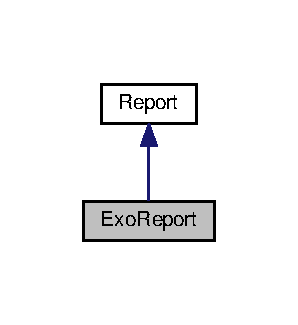
\includegraphics[width=143pt]{classExoReport__inherit__graph}
\end{center}
\end{figure}


Collaboration diagram for Exo\+Report\+:
\nopagebreak
\begin{figure}[H]
\begin{center}
\leavevmode
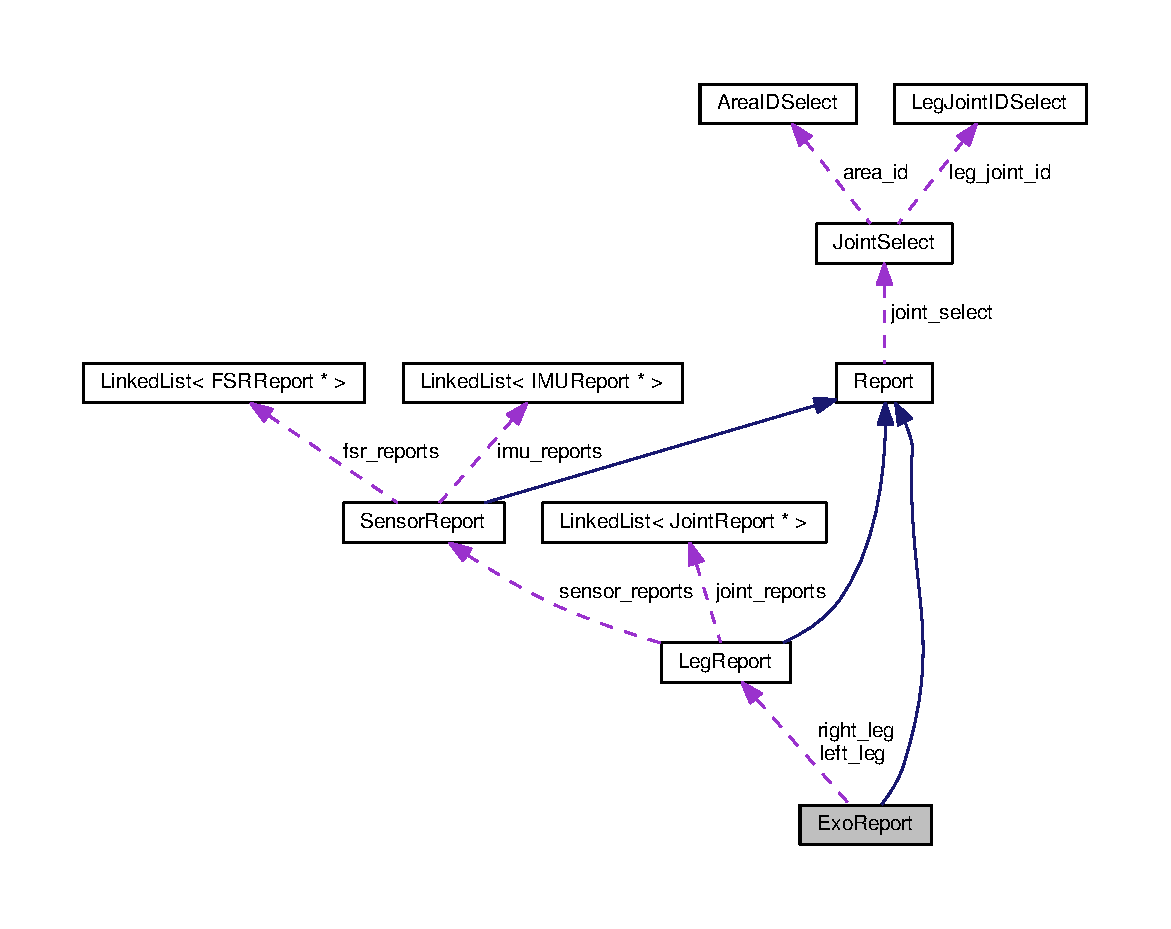
\includegraphics[width=350pt]{classExoReport__coll__graph}
\end{center}
\end{figure}
\subsection*{Public Member Functions}
\begin{DoxyCompactItemize}
\item 
\hyperlink{classExoReport_aa934ecdf4c20fa07e43bf9e89d0ecb71}{Exo\+Report} ()
\item 
\hyperlink{classExoReport_abfef51227b2ca8e38478fbb6db5b15af}{Exo\+Report} (\hyperlink{classLegReport}{Leg\+Report} $\ast$left, \hyperlink{classLegReport}{Leg\+Report} $\ast$right)
\item 
\hyperlink{classExoReport_ae33baafc0d7ed5198054a3874a700e1f}{$\sim$\+Exo\+Report} ()
\item 
\hyperlink{classLegReport}{Leg\+Report} $\ast$ \hyperlink{classExoReport_ab6b3930e8457d257ef6641247d0bf5bf}{get\+Area\+Report} (\hyperlink{JointSelect_8hpp_a0b0b6279ef5d4a446f8f07404dc868d3}{Area\+ID} id)
\end{DoxyCompactItemize}
\subsection*{Public Attributes}
\begin{DoxyCompactItemize}
\item 
\hyperlink{classLegReport}{Leg\+Report} $\ast$ \hyperlink{classExoReport_a246f0e7f3d659b0ad46589f0219b68f0}{left\+\_\+leg}
\item 
\hyperlink{classLegReport}{Leg\+Report} $\ast$ \hyperlink{classExoReport_af47a02ce1af583c62ee962100c7a8a73}{right\+\_\+leg}
\end{DoxyCompactItemize}


\subsection{Constructor \& Destructor Documentation}
\index{Exo\+Report@{Exo\+Report}!Exo\+Report@{Exo\+Report}}
\index{Exo\+Report@{Exo\+Report}!Exo\+Report@{Exo\+Report}}
\subsubsection[{\texorpdfstring{Exo\+Report()}{ExoReport()}}]{\setlength{\rightskip}{0pt plus 5cm}Exo\+Report\+::\+Exo\+Report (
\begin{DoxyParamCaption}
{}
\end{DoxyParamCaption}
)}\hypertarget{classExoReport_aa934ecdf4c20fa07e43bf9e89d0ecb71}{}\label{classExoReport_aa934ecdf4c20fa07e43bf9e89d0ecb71}
\index{Exo\+Report@{Exo\+Report}!Exo\+Report@{Exo\+Report}}
\index{Exo\+Report@{Exo\+Report}!Exo\+Report@{Exo\+Report}}
\subsubsection[{\texorpdfstring{Exo\+Report(\+Leg\+Report $\ast$left, Leg\+Report $\ast$right)}{ExoReport(LegReport *left, LegReport *right)}}]{\setlength{\rightskip}{0pt plus 5cm}Exo\+Report\+::\+Exo\+Report (
\begin{DoxyParamCaption}
\item[{{\bf Leg\+Report} $\ast$}]{left, }
\item[{{\bf Leg\+Report} $\ast$}]{right}
\end{DoxyParamCaption}
)}\hypertarget{classExoReport_abfef51227b2ca8e38478fbb6db5b15af}{}\label{classExoReport_abfef51227b2ca8e38478fbb6db5b15af}
\index{Exo\+Report@{Exo\+Report}!````~Exo\+Report@{$\sim$\+Exo\+Report}}
\index{````~Exo\+Report@{$\sim$\+Exo\+Report}!Exo\+Report@{Exo\+Report}}
\subsubsection[{\texorpdfstring{$\sim$\+Exo\+Report()}{~ExoReport()}}]{\setlength{\rightskip}{0pt plus 5cm}Exo\+Report\+::$\sim$\+Exo\+Report (
\begin{DoxyParamCaption}
{}
\end{DoxyParamCaption}
)}\hypertarget{classExoReport_ae33baafc0d7ed5198054a3874a700e1f}{}\label{classExoReport_ae33baafc0d7ed5198054a3874a700e1f}


\subsection{Member Function Documentation}
\index{Exo\+Report@{Exo\+Report}!get\+Area\+Report@{get\+Area\+Report}}
\index{get\+Area\+Report@{get\+Area\+Report}!Exo\+Report@{Exo\+Report}}
\subsubsection[{\texorpdfstring{get\+Area\+Report(\+Area\+I\+D id)}{getAreaReport(AreaID id)}}]{\setlength{\rightskip}{0pt plus 5cm}{\bf Leg\+Report} $\ast$ Exo\+Report\+::get\+Area\+Report (
\begin{DoxyParamCaption}
\item[{{\bf Area\+ID}}]{id}
\end{DoxyParamCaption}
)}\hypertarget{classExoReport_ab6b3930e8457d257ef6641247d0bf5bf}{}\label{classExoReport_ab6b3930e8457d257ef6641247d0bf5bf}


\subsection{Member Data Documentation}
\index{Exo\+Report@{Exo\+Report}!left\+\_\+leg@{left\+\_\+leg}}
\index{left\+\_\+leg@{left\+\_\+leg}!Exo\+Report@{Exo\+Report}}
\subsubsection[{\texorpdfstring{left\+\_\+leg}{left_leg}}]{\setlength{\rightskip}{0pt plus 5cm}{\bf Leg\+Report}$\ast$ Exo\+Report\+::left\+\_\+leg}\hypertarget{classExoReport_a246f0e7f3d659b0ad46589f0219b68f0}{}\label{classExoReport_a246f0e7f3d659b0ad46589f0219b68f0}
\index{Exo\+Report@{Exo\+Report}!right\+\_\+leg@{right\+\_\+leg}}
\index{right\+\_\+leg@{right\+\_\+leg}!Exo\+Report@{Exo\+Report}}
\subsubsection[{\texorpdfstring{right\+\_\+leg}{right_leg}}]{\setlength{\rightskip}{0pt plus 5cm}{\bf Leg\+Report}$\ast$ Exo\+Report\+::right\+\_\+leg}\hypertarget{classExoReport_af47a02ce1af583c62ee962100c7a8a73}{}\label{classExoReport_af47a02ce1af583c62ee962100c7a8a73}


The documentation for this class was generated from the following files\+:\begin{DoxyCompactItemize}
\item 
\hyperlink{Report_8hpp}{Report.\+hpp}\item 
\hyperlink{Report_8cpp}{Report.\+cpp}\end{DoxyCompactItemize}

\hypertarget{classExoReportBuilder}{}\section{Exo\+Report\+Builder Class Reference}
\label{classExoReportBuilder}\index{Exo\+Report\+Builder@{Exo\+Report\+Builder}}


{\ttfamily \#include $<$Report\+Builder.\+hpp$>$}

\subsection*{Public Member Functions}
\begin{DoxyCompactItemize}
\item 
\hyperlink{classExoReportBuilder_ae41848422d6c0566b822897a8d0a59fe}{Exo\+Report\+Builder} ()
\item 
void \hyperlink{classExoReportBuilder_ad642e5b66485b0124c43531cfb363d5f}{set\+Left\+Leg\+Report} (\hyperlink{classLegReport}{Leg\+Report} $\ast$left\+\_\+leg\+\_\+report)
\item 
void \hyperlink{classExoReportBuilder_a17d0f5a307fd0e6579f3245f71cf45a5}{set\+Right\+Leg\+Report} (\hyperlink{classLegReport}{Leg\+Report} $\ast$right\+\_\+leg\+\_\+report)
\item 
\hyperlink{classExoReport}{Exo\+Report} $\ast$ \hyperlink{classExoReportBuilder_a7c642afbbba7ea8160e36d045cacba67}{build} ()
\end{DoxyCompactItemize}


\subsection{Constructor \& Destructor Documentation}
\index{Exo\+Report\+Builder@{Exo\+Report\+Builder}!Exo\+Report\+Builder@{Exo\+Report\+Builder}}
\index{Exo\+Report\+Builder@{Exo\+Report\+Builder}!Exo\+Report\+Builder@{Exo\+Report\+Builder}}
\subsubsection[{\texorpdfstring{Exo\+Report\+Builder()}{ExoReportBuilder()}}]{\setlength{\rightskip}{0pt plus 5cm}Exo\+Report\+Builder\+::\+Exo\+Report\+Builder (
\begin{DoxyParamCaption}
{}
\end{DoxyParamCaption}
)}\hypertarget{classExoReportBuilder_ae41848422d6c0566b822897a8d0a59fe}{}\label{classExoReportBuilder_ae41848422d6c0566b822897a8d0a59fe}


\subsection{Member Function Documentation}
\index{Exo\+Report\+Builder@{Exo\+Report\+Builder}!build@{build}}
\index{build@{build}!Exo\+Report\+Builder@{Exo\+Report\+Builder}}
\subsubsection[{\texorpdfstring{build()}{build()}}]{\setlength{\rightskip}{0pt plus 5cm}{\bf Exo\+Report} $\ast$ Exo\+Report\+Builder\+::build (
\begin{DoxyParamCaption}
{}
\end{DoxyParamCaption}
)}\hypertarget{classExoReportBuilder_a7c642afbbba7ea8160e36d045cacba67}{}\label{classExoReportBuilder_a7c642afbbba7ea8160e36d045cacba67}
\index{Exo\+Report\+Builder@{Exo\+Report\+Builder}!set\+Left\+Leg\+Report@{set\+Left\+Leg\+Report}}
\index{set\+Left\+Leg\+Report@{set\+Left\+Leg\+Report}!Exo\+Report\+Builder@{Exo\+Report\+Builder}}
\subsubsection[{\texorpdfstring{set\+Left\+Leg\+Report(\+Leg\+Report $\ast$left\+\_\+leg\+\_\+report)}{setLeftLegReport(LegReport *left_leg_report)}}]{\setlength{\rightskip}{0pt plus 5cm}void Exo\+Report\+Builder\+::set\+Left\+Leg\+Report (
\begin{DoxyParamCaption}
\item[{{\bf Leg\+Report} $\ast$}]{left\+\_\+leg\+\_\+report}
\end{DoxyParamCaption}
)}\hypertarget{classExoReportBuilder_ad642e5b66485b0124c43531cfb363d5f}{}\label{classExoReportBuilder_ad642e5b66485b0124c43531cfb363d5f}
\index{Exo\+Report\+Builder@{Exo\+Report\+Builder}!set\+Right\+Leg\+Report@{set\+Right\+Leg\+Report}}
\index{set\+Right\+Leg\+Report@{set\+Right\+Leg\+Report}!Exo\+Report\+Builder@{Exo\+Report\+Builder}}
\subsubsection[{\texorpdfstring{set\+Right\+Leg\+Report(\+Leg\+Report $\ast$right\+\_\+leg\+\_\+report)}{setRightLegReport(LegReport *right_leg_report)}}]{\setlength{\rightskip}{0pt plus 5cm}void Exo\+Report\+Builder\+::set\+Right\+Leg\+Report (
\begin{DoxyParamCaption}
\item[{{\bf Leg\+Report} $\ast$}]{right\+\_\+leg\+\_\+report}
\end{DoxyParamCaption}
)}\hypertarget{classExoReportBuilder_a17d0f5a307fd0e6579f3245f71cf45a5}{}\label{classExoReportBuilder_a17d0f5a307fd0e6579f3245f71cf45a5}


The documentation for this class was generated from the following files\+:\begin{DoxyCompactItemize}
\item 
\hyperlink{ReportBuilder_8hpp}{Report\+Builder.\+hpp}\item 
\hyperlink{ReportBuilder_8cpp}{Report\+Builder.\+cpp}\end{DoxyCompactItemize}

\hypertarget{classExoskeleton}{}\section{Exoskeleton Class Reference}
\label{classExoskeleton}\index{Exoskeleton@{Exoskeleton}}


{\ttfamily \#include $<$Exoskeleton.\+hpp$>$}

\subsection*{Public Member Functions}
\begin{DoxyCompactItemize}
\item 
\hyperlink{classExoskeleton_ad8715617b3ba37cb31cbfa9679ec658f}{Exoskeleton} (\hyperlink{classLeg}{Leg} $\ast$left\+\_\+leg, \hyperlink{classLeg}{Leg} $\ast$right\+\_\+leg, \hyperlink{classCommunications}{Communications} $\ast$comms, \hyperlink{classOutputPort}{Output\+Port} $\ast$motor\+\_\+enable\+\_\+port, \hyperlink{classOutputPort}{Output\+Port} $\ast$led\+\_\+port)
\item 
\hyperlink{classExoskeleton_ae1c57b8f0c73de1ba90b0032d322a22e}{$\sim$\+Exoskeleton} ()
\item 
void \hyperlink{classExoskeleton_ac72f30ed64b121a89f546e542d3f4b70}{run} ()
\item 
void \hyperlink{classExoskeleton_a5c4a24e482efc10effd32ef3ae318843}{measure\+Sensors} ()
\item 
bool \hyperlink{classExoskeleton_af6caca71956f565f8c8f11f14b74ab48}{check\+Motor\+Errors} ()
\item 
void \hyperlink{classExoskeleton_af5a56800ab2bb98eae7e14470f4e91e0}{disable\+Exo} ()
\item 
void \hyperlink{classExoskeleton_a562adb009a9eb74d0b3197ff191561f2}{enable\+Exo} ()
\item 
void \hyperlink{classExoskeleton_a861d90cb9820ab25926391ad2c0a1509}{apply\+Torque} ()
\item 
void \hyperlink{classExoskeleton_a64f19c7f0a676342f12fbc000efce386}{adjust\+Control} ()
\item 
void \hyperlink{classExoskeleton_aae87818791c933e46ad9b991f5f54a31}{reset\+Starting\+Parameters} ()
\item 
void \hyperlink{classExoskeleton_a9af6d42deae939186da16188080f1bb4}{calibrate\+Torque} ()
\item 
void \hyperlink{classExoskeleton_a16374a659b52484ffd0b025778a0c1bb}{calibrate\+F\+S\+Rs} ()
\item 
void \hyperlink{classExoskeleton_ab5aaa55867ccf1ac42688f78b57e9f43}{set\+Zero\+If\+State\+State} ()
\item 
void \hyperlink{classExoskeleton_a3cbba1f7a77e5471787a5a777e8a557b}{calibrate\+I\+M\+Us} ()
\item 
void \hyperlink{classExoskeleton_aeff1385bc52343f715402cbc8eea5a31}{start\+Trial} ()
\item 
void \hyperlink{classExoskeleton_a931729600ee97d5bad706895c5d2d7c7}{end\+Trial} ()
\item 
void \hyperlink{classExoskeleton_a1d9f0d9439e4842d499ad58a03a147be}{receive\+Messages} ()
\item 
void \hyperlink{classExoskeleton_abb6349a44535117ad0f1f6896c05fd43}{check\+Reset} ()
\item 
void \hyperlink{classExoskeleton_a4b3d0bf5319e8fe06b69d31593aac46b}{send\+Report} ()
\item 
void \hyperlink{classExoskeleton_a0866b3df92b9579e260846727492cb8a}{process\+Message} (\hyperlink{classExoMessage}{Exo\+Message} $\ast$msg)
\item 
\hyperlink{classExoReport}{Exo\+Report} $\ast$ \hyperlink{classExoskeleton_acc42fc15c6ce8375f2bba6eb401e1dee}{generate\+Report} ()
\item 
void \hyperlink{classExoskeleton_af02ec7675f5e35d26e94f51024847285}{fill\+Report} (\hyperlink{classExoReport}{Exo\+Report} $\ast$report)
\end{DoxyCompactItemize}


\subsection{Constructor \& Destructor Documentation}
\index{Exoskeleton@{Exoskeleton}!Exoskeleton@{Exoskeleton}}
\index{Exoskeleton@{Exoskeleton}!Exoskeleton@{Exoskeleton}}
\subsubsection[{\texorpdfstring{Exoskeleton(\+Leg $\ast$left\+\_\+leg, Leg $\ast$right\+\_\+leg, Communications $\ast$comms, Output\+Port $\ast$motor\+\_\+enable\+\_\+port, Output\+Port $\ast$led\+\_\+port)}{Exoskeleton(Leg *left_leg, Leg *right_leg, Communications *comms, OutputPort *motor_enable_port, OutputPort *led_port)}}]{\setlength{\rightskip}{0pt plus 5cm}Exoskeleton\+::\+Exoskeleton (
\begin{DoxyParamCaption}
\item[{{\bf Leg} $\ast$}]{left\+\_\+leg, }
\item[{{\bf Leg} $\ast$}]{right\+\_\+leg, }
\item[{{\bf Communications} $\ast$}]{comms, }
\item[{{\bf Output\+Port} $\ast$}]{motor\+\_\+enable\+\_\+port, }
\item[{{\bf Output\+Port} $\ast$}]{led\+\_\+port}
\end{DoxyParamCaption}
)}\hypertarget{classExoskeleton_ad8715617b3ba37cb31cbfa9679ec658f}{}\label{classExoskeleton_ad8715617b3ba37cb31cbfa9679ec658f}
\index{Exoskeleton@{Exoskeleton}!````~Exoskeleton@{$\sim$\+Exoskeleton}}
\index{````~Exoskeleton@{$\sim$\+Exoskeleton}!Exoskeleton@{Exoskeleton}}
\subsubsection[{\texorpdfstring{$\sim$\+Exoskeleton()}{~Exoskeleton()}}]{\setlength{\rightskip}{0pt plus 5cm}Exoskeleton\+::$\sim$\+Exoskeleton (
\begin{DoxyParamCaption}
{}
\end{DoxyParamCaption}
)}\hypertarget{classExoskeleton_ae1c57b8f0c73de1ba90b0032d322a22e}{}\label{classExoskeleton_ae1c57b8f0c73de1ba90b0032d322a22e}


\subsection{Member Function Documentation}
\index{Exoskeleton@{Exoskeleton}!adjust\+Control@{adjust\+Control}}
\index{adjust\+Control@{adjust\+Control}!Exoskeleton@{Exoskeleton}}
\subsubsection[{\texorpdfstring{adjust\+Control()}{adjustControl()}}]{\setlength{\rightskip}{0pt plus 5cm}void Exoskeleton\+::adjust\+Control (
\begin{DoxyParamCaption}
{}
\end{DoxyParamCaption}
)}\hypertarget{classExoskeleton_a64f19c7f0a676342f12fbc000efce386}{}\label{classExoskeleton_a64f19c7f0a676342f12fbc000efce386}
\index{Exoskeleton@{Exoskeleton}!apply\+Torque@{apply\+Torque}}
\index{apply\+Torque@{apply\+Torque}!Exoskeleton@{Exoskeleton}}
\subsubsection[{\texorpdfstring{apply\+Torque()}{applyTorque()}}]{\setlength{\rightskip}{0pt plus 5cm}void Exoskeleton\+::apply\+Torque (
\begin{DoxyParamCaption}
{}
\end{DoxyParamCaption}
)}\hypertarget{classExoskeleton_a861d90cb9820ab25926391ad2c0a1509}{}\label{classExoskeleton_a861d90cb9820ab25926391ad2c0a1509}
\index{Exoskeleton@{Exoskeleton}!calibrate\+F\+S\+Rs@{calibrate\+F\+S\+Rs}}
\index{calibrate\+F\+S\+Rs@{calibrate\+F\+S\+Rs}!Exoskeleton@{Exoskeleton}}
\subsubsection[{\texorpdfstring{calibrate\+F\+S\+Rs()}{calibrateFSRs()}}]{\setlength{\rightskip}{0pt plus 5cm}void Exoskeleton\+::calibrate\+F\+S\+Rs (
\begin{DoxyParamCaption}
{}
\end{DoxyParamCaption}
)}\hypertarget{classExoskeleton_a16374a659b52484ffd0b025778a0c1bb}{}\label{classExoskeleton_a16374a659b52484ffd0b025778a0c1bb}
\index{Exoskeleton@{Exoskeleton}!calibrate\+I\+M\+Us@{calibrate\+I\+M\+Us}}
\index{calibrate\+I\+M\+Us@{calibrate\+I\+M\+Us}!Exoskeleton@{Exoskeleton}}
\subsubsection[{\texorpdfstring{calibrate\+I\+M\+Us()}{calibrateIMUs()}}]{\setlength{\rightskip}{0pt plus 5cm}void Exoskeleton\+::calibrate\+I\+M\+Us (
\begin{DoxyParamCaption}
{}
\end{DoxyParamCaption}
)}\hypertarget{classExoskeleton_a3cbba1f7a77e5471787a5a777e8a557b}{}\label{classExoskeleton_a3cbba1f7a77e5471787a5a777e8a557b}
\index{Exoskeleton@{Exoskeleton}!calibrate\+Torque@{calibrate\+Torque}}
\index{calibrate\+Torque@{calibrate\+Torque}!Exoskeleton@{Exoskeleton}}
\subsubsection[{\texorpdfstring{calibrate\+Torque()}{calibrateTorque()}}]{\setlength{\rightskip}{0pt plus 5cm}void Exoskeleton\+::calibrate\+Torque (
\begin{DoxyParamCaption}
{}
\end{DoxyParamCaption}
)}\hypertarget{classExoskeleton_a9af6d42deae939186da16188080f1bb4}{}\label{classExoskeleton_a9af6d42deae939186da16188080f1bb4}
\index{Exoskeleton@{Exoskeleton}!check\+Motor\+Errors@{check\+Motor\+Errors}}
\index{check\+Motor\+Errors@{check\+Motor\+Errors}!Exoskeleton@{Exoskeleton}}
\subsubsection[{\texorpdfstring{check\+Motor\+Errors()}{checkMotorErrors()}}]{\setlength{\rightskip}{0pt plus 5cm}bool Exoskeleton\+::check\+Motor\+Errors (
\begin{DoxyParamCaption}
{}
\end{DoxyParamCaption}
)}\hypertarget{classExoskeleton_af6caca71956f565f8c8f11f14b74ab48}{}\label{classExoskeleton_af6caca71956f565f8c8f11f14b74ab48}
\index{Exoskeleton@{Exoskeleton}!check\+Reset@{check\+Reset}}
\index{check\+Reset@{check\+Reset}!Exoskeleton@{Exoskeleton}}
\subsubsection[{\texorpdfstring{check\+Reset()}{checkReset()}}]{\setlength{\rightskip}{0pt plus 5cm}void Exoskeleton\+::check\+Reset (
\begin{DoxyParamCaption}
{}
\end{DoxyParamCaption}
)}\hypertarget{classExoskeleton_abb6349a44535117ad0f1f6896c05fd43}{}\label{classExoskeleton_abb6349a44535117ad0f1f6896c05fd43}
\index{Exoskeleton@{Exoskeleton}!disable\+Exo@{disable\+Exo}}
\index{disable\+Exo@{disable\+Exo}!Exoskeleton@{Exoskeleton}}
\subsubsection[{\texorpdfstring{disable\+Exo()}{disableExo()}}]{\setlength{\rightskip}{0pt plus 5cm}void Exoskeleton\+::disable\+Exo (
\begin{DoxyParamCaption}
{}
\end{DoxyParamCaption}
)}\hypertarget{classExoskeleton_af5a56800ab2bb98eae7e14470f4e91e0}{}\label{classExoskeleton_af5a56800ab2bb98eae7e14470f4e91e0}
\index{Exoskeleton@{Exoskeleton}!enable\+Exo@{enable\+Exo}}
\index{enable\+Exo@{enable\+Exo}!Exoskeleton@{Exoskeleton}}
\subsubsection[{\texorpdfstring{enable\+Exo()}{enableExo()}}]{\setlength{\rightskip}{0pt plus 5cm}void Exoskeleton\+::enable\+Exo (
\begin{DoxyParamCaption}
{}
\end{DoxyParamCaption}
)}\hypertarget{classExoskeleton_a562adb009a9eb74d0b3197ff191561f2}{}\label{classExoskeleton_a562adb009a9eb74d0b3197ff191561f2}
\index{Exoskeleton@{Exoskeleton}!end\+Trial@{end\+Trial}}
\index{end\+Trial@{end\+Trial}!Exoskeleton@{Exoskeleton}}
\subsubsection[{\texorpdfstring{end\+Trial()}{endTrial()}}]{\setlength{\rightskip}{0pt plus 5cm}void Exoskeleton\+::end\+Trial (
\begin{DoxyParamCaption}
{}
\end{DoxyParamCaption}
)}\hypertarget{classExoskeleton_a931729600ee97d5bad706895c5d2d7c7}{}\label{classExoskeleton_a931729600ee97d5bad706895c5d2d7c7}
\index{Exoskeleton@{Exoskeleton}!fill\+Report@{fill\+Report}}
\index{fill\+Report@{fill\+Report}!Exoskeleton@{Exoskeleton}}
\subsubsection[{\texorpdfstring{fill\+Report(\+Exo\+Report $\ast$report)}{fillReport(ExoReport *report)}}]{\setlength{\rightskip}{0pt plus 5cm}void Exoskeleton\+::fill\+Report (
\begin{DoxyParamCaption}
\item[{{\bf Exo\+Report} $\ast$}]{report}
\end{DoxyParamCaption}
)}\hypertarget{classExoskeleton_af02ec7675f5e35d26e94f51024847285}{}\label{classExoskeleton_af02ec7675f5e35d26e94f51024847285}
\index{Exoskeleton@{Exoskeleton}!generate\+Report@{generate\+Report}}
\index{generate\+Report@{generate\+Report}!Exoskeleton@{Exoskeleton}}
\subsubsection[{\texorpdfstring{generate\+Report()}{generateReport()}}]{\setlength{\rightskip}{0pt plus 5cm}{\bf Exo\+Report} $\ast$ Exoskeleton\+::generate\+Report (
\begin{DoxyParamCaption}
{}
\end{DoxyParamCaption}
)}\hypertarget{classExoskeleton_acc42fc15c6ce8375f2bba6eb401e1dee}{}\label{classExoskeleton_acc42fc15c6ce8375f2bba6eb401e1dee}
\index{Exoskeleton@{Exoskeleton}!measure\+Sensors@{measure\+Sensors}}
\index{measure\+Sensors@{measure\+Sensors}!Exoskeleton@{Exoskeleton}}
\subsubsection[{\texorpdfstring{measure\+Sensors()}{measureSensors()}}]{\setlength{\rightskip}{0pt plus 5cm}void Exoskeleton\+::measure\+Sensors (
\begin{DoxyParamCaption}
{}
\end{DoxyParamCaption}
)}\hypertarget{classExoskeleton_a5c4a24e482efc10effd32ef3ae318843}{}\label{classExoskeleton_a5c4a24e482efc10effd32ef3ae318843}
\index{Exoskeleton@{Exoskeleton}!process\+Message@{process\+Message}}
\index{process\+Message@{process\+Message}!Exoskeleton@{Exoskeleton}}
\subsubsection[{\texorpdfstring{process\+Message(\+Exo\+Message $\ast$msg)}{processMessage(ExoMessage *msg)}}]{\setlength{\rightskip}{0pt plus 5cm}void Exoskeleton\+::process\+Message (
\begin{DoxyParamCaption}
\item[{{\bf Exo\+Message} $\ast$}]{msg}
\end{DoxyParamCaption}
)}\hypertarget{classExoskeleton_a0866b3df92b9579e260846727492cb8a}{}\label{classExoskeleton_a0866b3df92b9579e260846727492cb8a}
\index{Exoskeleton@{Exoskeleton}!receive\+Messages@{receive\+Messages}}
\index{receive\+Messages@{receive\+Messages}!Exoskeleton@{Exoskeleton}}
\subsubsection[{\texorpdfstring{receive\+Messages()}{receiveMessages()}}]{\setlength{\rightskip}{0pt plus 5cm}void Exoskeleton\+::receive\+Messages (
\begin{DoxyParamCaption}
{}
\end{DoxyParamCaption}
)}\hypertarget{classExoskeleton_a1d9f0d9439e4842d499ad58a03a147be}{}\label{classExoskeleton_a1d9f0d9439e4842d499ad58a03a147be}
\index{Exoskeleton@{Exoskeleton}!reset\+Starting\+Parameters@{reset\+Starting\+Parameters}}
\index{reset\+Starting\+Parameters@{reset\+Starting\+Parameters}!Exoskeleton@{Exoskeleton}}
\subsubsection[{\texorpdfstring{reset\+Starting\+Parameters()}{resetStartingParameters()}}]{\setlength{\rightskip}{0pt plus 5cm}void Exoskeleton\+::reset\+Starting\+Parameters (
\begin{DoxyParamCaption}
{}
\end{DoxyParamCaption}
)}\hypertarget{classExoskeleton_aae87818791c933e46ad9b991f5f54a31}{}\label{classExoskeleton_aae87818791c933e46ad9b991f5f54a31}
\index{Exoskeleton@{Exoskeleton}!run@{run}}
\index{run@{run}!Exoskeleton@{Exoskeleton}}
\subsubsection[{\texorpdfstring{run()}{run()}}]{\setlength{\rightskip}{0pt plus 5cm}void Exoskeleton\+::run (
\begin{DoxyParamCaption}
{}
\end{DoxyParamCaption}
)}\hypertarget{classExoskeleton_ac72f30ed64b121a89f546e542d3f4b70}{}\label{classExoskeleton_ac72f30ed64b121a89f546e542d3f4b70}
\index{Exoskeleton@{Exoskeleton}!send\+Report@{send\+Report}}
\index{send\+Report@{send\+Report}!Exoskeleton@{Exoskeleton}}
\subsubsection[{\texorpdfstring{send\+Report()}{sendReport()}}]{\setlength{\rightskip}{0pt plus 5cm}void Exoskeleton\+::send\+Report (
\begin{DoxyParamCaption}
{}
\end{DoxyParamCaption}
)}\hypertarget{classExoskeleton_a4b3d0bf5319e8fe06b69d31593aac46b}{}\label{classExoskeleton_a4b3d0bf5319e8fe06b69d31593aac46b}
\index{Exoskeleton@{Exoskeleton}!set\+Zero\+If\+State\+State@{set\+Zero\+If\+State\+State}}
\index{set\+Zero\+If\+State\+State@{set\+Zero\+If\+State\+State}!Exoskeleton@{Exoskeleton}}
\subsubsection[{\texorpdfstring{set\+Zero\+If\+State\+State()}{setZeroIfStateState()}}]{\setlength{\rightskip}{0pt plus 5cm}void Exoskeleton\+::set\+Zero\+If\+State\+State (
\begin{DoxyParamCaption}
{}
\end{DoxyParamCaption}
)}\hypertarget{classExoskeleton_ab5aaa55867ccf1ac42688f78b57e9f43}{}\label{classExoskeleton_ab5aaa55867ccf1ac42688f78b57e9f43}
\index{Exoskeleton@{Exoskeleton}!start\+Trial@{start\+Trial}}
\index{start\+Trial@{start\+Trial}!Exoskeleton@{Exoskeleton}}
\subsubsection[{\texorpdfstring{start\+Trial()}{startTrial()}}]{\setlength{\rightskip}{0pt plus 5cm}void Exoskeleton\+::start\+Trial (
\begin{DoxyParamCaption}
{}
\end{DoxyParamCaption}
)}\hypertarget{classExoskeleton_aeff1385bc52343f715402cbc8eea5a31}{}\label{classExoskeleton_aeff1385bc52343f715402cbc8eea5a31}


The documentation for this class was generated from the following files\+:\begin{DoxyCompactItemize}
\item 
\hyperlink{Exoskeleton_8hpp}{Exoskeleton.\+hpp}\item 
\hyperlink{Exoskeleton_8cpp}{Exoskeleton.\+cpp}\end{DoxyCompactItemize}

\hypertarget{classFSR}{}\section{F\+SR Class Reference}
\label{classFSR}\index{F\+SR@{F\+SR}}


{\ttfamily \#include $<$F\+S\+R.\+hpp$>$}



Inheritance diagram for F\+SR\+:\nopagebreak
\begin{figure}[H]
\begin{center}
\leavevmode
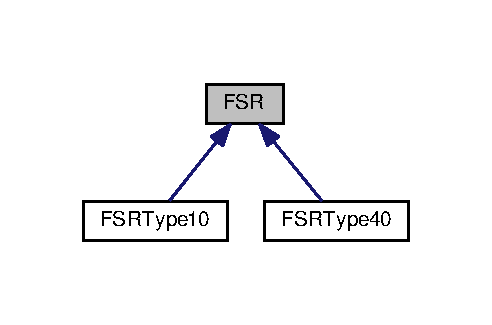
\includegraphics[width=236pt]{classFSR__inherit__graph}
\end{center}
\end{figure}
\subsection*{Public Member Functions}
\begin{DoxyCompactItemize}
\item 
\hyperlink{classFSR_a60affe23db0aad2dfb0d0a233846b81e}{F\+SR} (\hyperlink{classInputPort}{Input\+Port} $\ast$port)
\item 
virtual \hyperlink{classFSR_a492baa895ecf45ae284902f2344902a4}{$\sim$\+F\+SR} ()
\item 
void \hyperlink{classFSR_acb1a2519baa15b75d691d54cd6d08c4a}{measure\+Force} ()
\item 
double \hyperlink{classFSR_a8666ee8398acf01f62792c87f75b4444}{get\+Force} ()
\item 
void \hyperlink{classFSR_ac05f6399106a78a9062673ef80c1d423}{calibrate} ()
\item 
void \hyperlink{classFSR_a94049f17889fd17af537bb87a8657a73}{reset\+Maxes} ()
\end{DoxyCompactItemize}


\subsection{Constructor \& Destructor Documentation}
\index{F\+SR@{F\+SR}!F\+SR@{F\+SR}}
\index{F\+SR@{F\+SR}!F\+SR@{F\+SR}}
\subsubsection[{\texorpdfstring{F\+S\+R(\+Input\+Port $\ast$port)}{FSR(InputPort *port)}}]{\setlength{\rightskip}{0pt plus 5cm}F\+S\+R\+::\+F\+SR (
\begin{DoxyParamCaption}
\item[{{\bf Input\+Port} $\ast$}]{port}
\end{DoxyParamCaption}
)}\hypertarget{classFSR_a60affe23db0aad2dfb0d0a233846b81e}{}\label{classFSR_a60affe23db0aad2dfb0d0a233846b81e}
\index{F\+SR@{F\+SR}!````~F\+SR@{$\sim$\+F\+SR}}
\index{````~F\+SR@{$\sim$\+F\+SR}!F\+SR@{F\+SR}}
\subsubsection[{\texorpdfstring{$\sim$\+F\+S\+R()}{~FSR()}}]{\setlength{\rightskip}{0pt plus 5cm}F\+S\+R\+::$\sim$\+F\+SR (
\begin{DoxyParamCaption}
{}
\end{DoxyParamCaption}
)\hspace{0.3cm}{\ttfamily [virtual]}}\hypertarget{classFSR_a492baa895ecf45ae284902f2344902a4}{}\label{classFSR_a492baa895ecf45ae284902f2344902a4}


\subsection{Member Function Documentation}
\index{F\+SR@{F\+SR}!calibrate@{calibrate}}
\index{calibrate@{calibrate}!F\+SR@{F\+SR}}
\subsubsection[{\texorpdfstring{calibrate()}{calibrate()}}]{\setlength{\rightskip}{0pt plus 5cm}void F\+S\+R\+::calibrate (
\begin{DoxyParamCaption}
{}
\end{DoxyParamCaption}
)}\hypertarget{classFSR_ac05f6399106a78a9062673ef80c1d423}{}\label{classFSR_ac05f6399106a78a9062673ef80c1d423}
\index{F\+SR@{F\+SR}!get\+Force@{get\+Force}}
\index{get\+Force@{get\+Force}!F\+SR@{F\+SR}}
\subsubsection[{\texorpdfstring{get\+Force()}{getForce()}}]{\setlength{\rightskip}{0pt plus 5cm}double F\+S\+R\+::get\+Force (
\begin{DoxyParamCaption}
{}
\end{DoxyParamCaption}
)}\hypertarget{classFSR_a8666ee8398acf01f62792c87f75b4444}{}\label{classFSR_a8666ee8398acf01f62792c87f75b4444}
\index{F\+SR@{F\+SR}!measure\+Force@{measure\+Force}}
\index{measure\+Force@{measure\+Force}!F\+SR@{F\+SR}}
\subsubsection[{\texorpdfstring{measure\+Force()}{measureForce()}}]{\setlength{\rightskip}{0pt plus 5cm}void F\+S\+R\+::measure\+Force (
\begin{DoxyParamCaption}
{}
\end{DoxyParamCaption}
)}\hypertarget{classFSR_acb1a2519baa15b75d691d54cd6d08c4a}{}\label{classFSR_acb1a2519baa15b75d691d54cd6d08c4a}
\index{F\+SR@{F\+SR}!reset\+Maxes@{reset\+Maxes}}
\index{reset\+Maxes@{reset\+Maxes}!F\+SR@{F\+SR}}
\subsubsection[{\texorpdfstring{reset\+Maxes()}{resetMaxes()}}]{\setlength{\rightskip}{0pt plus 5cm}void F\+S\+R\+::reset\+Maxes (
\begin{DoxyParamCaption}
{}
\end{DoxyParamCaption}
)}\hypertarget{classFSR_a94049f17889fd17af537bb87a8657a73}{}\label{classFSR_a94049f17889fd17af537bb87a8657a73}


The documentation for this class was generated from the following files\+:\begin{DoxyCompactItemize}
\item 
\hyperlink{FSR_8hpp}{F\+S\+R.\+hpp}\item 
\hyperlink{FSR_8cpp}{F\+S\+R.\+cpp}\end{DoxyCompactItemize}

\hypertarget{classFsrFactory}{}\section{Fsr\+Factory Class Reference}
\label{classFsrFactory}\index{Fsr\+Factory@{Fsr\+Factory}}


{\ttfamily \#include $<$F\+S\+R.\+hpp$>$}

\subsection*{Public Member Functions}
\begin{DoxyCompactItemize}
\item 
\hyperlink{classFsrFactory_ab813e2ef246d2bcbebd2591c725f9eea}{Fsr\+Factory} (int type)
\item 
\hyperlink{classFSR}{F\+SR} $\ast$ \hyperlink{classFsrFactory_a817aad39b35e2c4bf0143b0b67851287}{create\+F\+SR} (\hyperlink{classInputPort}{Input\+Port} $\ast$port)
\end{DoxyCompactItemize}


\subsection{Constructor \& Destructor Documentation}
\index{Fsr\+Factory@{Fsr\+Factory}!Fsr\+Factory@{Fsr\+Factory}}
\index{Fsr\+Factory@{Fsr\+Factory}!Fsr\+Factory@{Fsr\+Factory}}
\subsubsection[{\texorpdfstring{Fsr\+Factory(int type)}{FsrFactory(int type)}}]{\setlength{\rightskip}{0pt plus 5cm}Fsr\+Factory\+::\+Fsr\+Factory (
\begin{DoxyParamCaption}
\item[{int}]{type}
\end{DoxyParamCaption}
)}\hypertarget{classFsrFactory_ab813e2ef246d2bcbebd2591c725f9eea}{}\label{classFsrFactory_ab813e2ef246d2bcbebd2591c725f9eea}


\subsection{Member Function Documentation}
\index{Fsr\+Factory@{Fsr\+Factory}!create\+F\+SR@{create\+F\+SR}}
\index{create\+F\+SR@{create\+F\+SR}!Fsr\+Factory@{Fsr\+Factory}}
\subsubsection[{\texorpdfstring{create\+F\+S\+R(\+Input\+Port $\ast$port)}{createFSR(InputPort *port)}}]{\setlength{\rightskip}{0pt plus 5cm}{\bf F\+SR} $\ast$ Fsr\+Factory\+::create\+F\+SR (
\begin{DoxyParamCaption}
\item[{{\bf Input\+Port} $\ast$}]{port}
\end{DoxyParamCaption}
)}\hypertarget{classFsrFactory_a817aad39b35e2c4bf0143b0b67851287}{}\label{classFsrFactory_a817aad39b35e2c4bf0143b0b67851287}


The documentation for this class was generated from the following files\+:\begin{DoxyCompactItemize}
\item 
\hyperlink{FSR_8hpp}{F\+S\+R.\+hpp}\item 
\hyperlink{FSR_8cpp}{F\+S\+R.\+cpp}\end{DoxyCompactItemize}

\hypertarget{classFSRGroup}{}\section{F\+S\+R\+Group Class Reference}
\label{classFSRGroup}\index{F\+S\+R\+Group@{F\+S\+R\+Group}}


{\ttfamily \#include $<$F\+S\+R.\+hpp$>$}



Inheritance diagram for F\+S\+R\+Group\+:\nopagebreak
\begin{figure}[H]
\begin{center}
\leavevmode
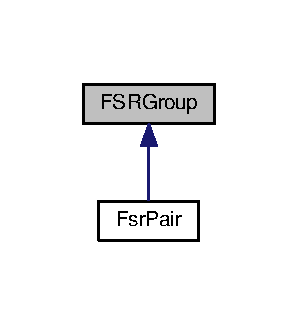
\includegraphics[width=143pt]{classFSRGroup__inherit__graph}
\end{center}
\end{figure}


Collaboration diagram for F\+S\+R\+Group\+:
\nopagebreak
\begin{figure}[H]
\begin{center}
\leavevmode
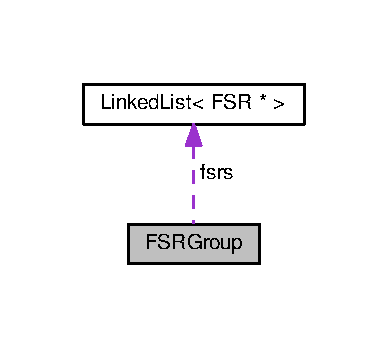
\includegraphics[width=186pt]{classFSRGroup__coll__graph}
\end{center}
\end{figure}
\subsection*{Public Member Functions}
\begin{DoxyCompactItemize}
\item 
\hyperlink{classFSRGroup_a14f2398406fea72cc9c42fe38a5209df}{F\+S\+R\+Group} (\hyperlink{classLinkedList}{Linked\+List}$<$ \hyperlink{classFSR}{F\+SR} $\ast$ $>$ $\ast$\hyperlink{classFSRGroup_a818ff1c99f2f1aaa5bd36c6cb701b491}{fsrs})
\item 
virtual \hyperlink{classFSRGroup_ace5505a55102264e6bba241f41ab4836}{$\sim$\+F\+S\+R\+Group} ()
\item 
bool \hyperlink{classFSRGroup_a6f60094985663d5a19c42b1f402d42e8}{is\+Activated} ()
\item 
void \hyperlink{classFSRGroup_a3af851fc34ba3aa756345a6c2cc488c4}{measure\+Force} ()
\item 
double \hyperlink{classFSRGroup_a69a95934d542076c08e049e3b0312994}{get\+Force} ()
\item 
void \hyperlink{classFSRGroup_a58d86b5460cecb3c006aecfda1dc43ec}{calibrate} ()
\item 
double \hyperlink{classFSRGroup_ab8266f4e3ef2bf17a71e59069ff35754}{get\+Threshold} ()
\item 
void \hyperlink{classFSRGroup_a9d9e243ad7f7368493c7cf6bf045e54b}{set\+Percentage\+Threshold} (double percent)
\item 
void \hyperlink{classFSRGroup_afb080b398697513ea57374be3c14bc6e}{reset\+Maxes} ()
\item 
void \hyperlink{classFSRGroup_a8c308ccc00dfe0e999c1e3deb06755be}{update\+Maxes} ()
\item 
double \hyperlink{classFSRGroup_a261c1a4bf8fd1ebd9237ec9d1b1b261f}{get\+Percentage} ()
\item 
double \hyperlink{classFSRGroup_a095df087d7140fdaa1240150a3b8acda}{get\+Max\+Percentage} ()
\item 
void \hyperlink{classFSRGroup_a8896f4f0b2b8b150a1ccff0ee303248a}{update\+Baseline} ()
\item 
\hyperlink{classFSRReport}{F\+S\+R\+Report} $\ast$ \hyperlink{classFSRGroup_a791432248f8a588adc292c0eb9e19c38}{generate\+Report} ()
\item 
virtual double \hyperlink{classFSRGroup_ae1658e0276de8cf7d9a3c29c84257d3b}{get\+Ratio} ()
\item 
virtual double \hyperlink{classFSRGroup_ab12866c42645b5d892a1d69fb7056e4f}{get\+Difference} ()
\item 
void \hyperlink{classFSRGroup_a5a59a5ddf09a579d693e1c3687fbff46}{fill\+Report} (\hyperlink{classFSRReport}{F\+S\+R\+Report} $\ast$report)
\end{DoxyCompactItemize}
\subsection*{Protected Attributes}
\begin{DoxyCompactItemize}
\item 
\hyperlink{classLinkedList}{Linked\+List}$<$ \hyperlink{classFSR}{F\+SR} $\ast$ $>$ \hyperlink{classFSRGroup_a818ff1c99f2f1aaa5bd36c6cb701b491}{fsrs}
\end{DoxyCompactItemize}


\subsection{Constructor \& Destructor Documentation}
\index{F\+S\+R\+Group@{F\+S\+R\+Group}!F\+S\+R\+Group@{F\+S\+R\+Group}}
\index{F\+S\+R\+Group@{F\+S\+R\+Group}!F\+S\+R\+Group@{F\+S\+R\+Group}}
\subsubsection[{\texorpdfstring{F\+S\+R\+Group(\+Linked\+List$<$ F\+S\+R $\ast$ $>$ $\ast$fsrs)}{FSRGroup(LinkedList< FSR * > *fsrs)}}]{\setlength{\rightskip}{0pt plus 5cm}F\+S\+R\+Group\+::\+F\+S\+R\+Group (
\begin{DoxyParamCaption}
\item[{{\bf Linked\+List}$<$ {\bf F\+SR} $\ast$ $>$ $\ast$}]{fsrs}
\end{DoxyParamCaption}
)}\hypertarget{classFSRGroup_a14f2398406fea72cc9c42fe38a5209df}{}\label{classFSRGroup_a14f2398406fea72cc9c42fe38a5209df}
\index{F\+S\+R\+Group@{F\+S\+R\+Group}!````~F\+S\+R\+Group@{$\sim$\+F\+S\+R\+Group}}
\index{````~F\+S\+R\+Group@{$\sim$\+F\+S\+R\+Group}!F\+S\+R\+Group@{F\+S\+R\+Group}}
\subsubsection[{\texorpdfstring{$\sim$\+F\+S\+R\+Group()}{~FSRGroup()}}]{\setlength{\rightskip}{0pt plus 5cm}F\+S\+R\+Group\+::$\sim$\+F\+S\+R\+Group (
\begin{DoxyParamCaption}
{}
\end{DoxyParamCaption}
)\hspace{0.3cm}{\ttfamily [virtual]}}\hypertarget{classFSRGroup_ace5505a55102264e6bba241f41ab4836}{}\label{classFSRGroup_ace5505a55102264e6bba241f41ab4836}


\subsection{Member Function Documentation}
\index{F\+S\+R\+Group@{F\+S\+R\+Group}!calibrate@{calibrate}}
\index{calibrate@{calibrate}!F\+S\+R\+Group@{F\+S\+R\+Group}}
\subsubsection[{\texorpdfstring{calibrate()}{calibrate()}}]{\setlength{\rightskip}{0pt plus 5cm}void F\+S\+R\+Group\+::calibrate (
\begin{DoxyParamCaption}
{}
\end{DoxyParamCaption}
)}\hypertarget{classFSRGroup_a58d86b5460cecb3c006aecfda1dc43ec}{}\label{classFSRGroup_a58d86b5460cecb3c006aecfda1dc43ec}
\index{F\+S\+R\+Group@{F\+S\+R\+Group}!fill\+Report@{fill\+Report}}
\index{fill\+Report@{fill\+Report}!F\+S\+R\+Group@{F\+S\+R\+Group}}
\subsubsection[{\texorpdfstring{fill\+Report(\+F\+S\+R\+Report $\ast$report)}{fillReport(FSRReport *report)}}]{\setlength{\rightskip}{0pt plus 5cm}void F\+S\+R\+Group\+::fill\+Report (
\begin{DoxyParamCaption}
\item[{{\bf F\+S\+R\+Report} $\ast$}]{report}
\end{DoxyParamCaption}
)}\hypertarget{classFSRGroup_a5a59a5ddf09a579d693e1c3687fbff46}{}\label{classFSRGroup_a5a59a5ddf09a579d693e1c3687fbff46}
\index{F\+S\+R\+Group@{F\+S\+R\+Group}!generate\+Report@{generate\+Report}}
\index{generate\+Report@{generate\+Report}!F\+S\+R\+Group@{F\+S\+R\+Group}}
\subsubsection[{\texorpdfstring{generate\+Report()}{generateReport()}}]{\setlength{\rightskip}{0pt plus 5cm}{\bf F\+S\+R\+Report} $\ast$ F\+S\+R\+Group\+::generate\+Report (
\begin{DoxyParamCaption}
{}
\end{DoxyParamCaption}
)}\hypertarget{classFSRGroup_a791432248f8a588adc292c0eb9e19c38}{}\label{classFSRGroup_a791432248f8a588adc292c0eb9e19c38}
\index{F\+S\+R\+Group@{F\+S\+R\+Group}!get\+Difference@{get\+Difference}}
\index{get\+Difference@{get\+Difference}!F\+S\+R\+Group@{F\+S\+R\+Group}}
\subsubsection[{\texorpdfstring{get\+Difference()}{getDifference()}}]{\setlength{\rightskip}{0pt plus 5cm}double F\+S\+R\+Group\+::get\+Difference (
\begin{DoxyParamCaption}
{}
\end{DoxyParamCaption}
)\hspace{0.3cm}{\ttfamily [virtual]}}\hypertarget{classFSRGroup_ab12866c42645b5d892a1d69fb7056e4f}{}\label{classFSRGroup_ab12866c42645b5d892a1d69fb7056e4f}


Reimplemented in \hyperlink{classFsrPair_aecd1acaffcf8a0c3ab60d1ddd2ac52bc}{Fsr\+Pair}.

\index{F\+S\+R\+Group@{F\+S\+R\+Group}!get\+Force@{get\+Force}}
\index{get\+Force@{get\+Force}!F\+S\+R\+Group@{F\+S\+R\+Group}}
\subsubsection[{\texorpdfstring{get\+Force()}{getForce()}}]{\setlength{\rightskip}{0pt plus 5cm}double F\+S\+R\+Group\+::get\+Force (
\begin{DoxyParamCaption}
{}
\end{DoxyParamCaption}
)}\hypertarget{classFSRGroup_a69a95934d542076c08e049e3b0312994}{}\label{classFSRGroup_a69a95934d542076c08e049e3b0312994}
\index{F\+S\+R\+Group@{F\+S\+R\+Group}!get\+Max\+Percentage@{get\+Max\+Percentage}}
\index{get\+Max\+Percentage@{get\+Max\+Percentage}!F\+S\+R\+Group@{F\+S\+R\+Group}}
\subsubsection[{\texorpdfstring{get\+Max\+Percentage()}{getMaxPercentage()}}]{\setlength{\rightskip}{0pt plus 5cm}double F\+S\+R\+Group\+::get\+Max\+Percentage (
\begin{DoxyParamCaption}
{}
\end{DoxyParamCaption}
)}\hypertarget{classFSRGroup_a095df087d7140fdaa1240150a3b8acda}{}\label{classFSRGroup_a095df087d7140fdaa1240150a3b8acda}
\index{F\+S\+R\+Group@{F\+S\+R\+Group}!get\+Percentage@{get\+Percentage}}
\index{get\+Percentage@{get\+Percentage}!F\+S\+R\+Group@{F\+S\+R\+Group}}
\subsubsection[{\texorpdfstring{get\+Percentage()}{getPercentage()}}]{\setlength{\rightskip}{0pt plus 5cm}double F\+S\+R\+Group\+::get\+Percentage (
\begin{DoxyParamCaption}
{}
\end{DoxyParamCaption}
)}\hypertarget{classFSRGroup_a261c1a4bf8fd1ebd9237ec9d1b1b261f}{}\label{classFSRGroup_a261c1a4bf8fd1ebd9237ec9d1b1b261f}
\index{F\+S\+R\+Group@{F\+S\+R\+Group}!get\+Ratio@{get\+Ratio}}
\index{get\+Ratio@{get\+Ratio}!F\+S\+R\+Group@{F\+S\+R\+Group}}
\subsubsection[{\texorpdfstring{get\+Ratio()}{getRatio()}}]{\setlength{\rightskip}{0pt plus 5cm}double F\+S\+R\+Group\+::get\+Ratio (
\begin{DoxyParamCaption}
{}
\end{DoxyParamCaption}
)\hspace{0.3cm}{\ttfamily [virtual]}}\hypertarget{classFSRGroup_ae1658e0276de8cf7d9a3c29c84257d3b}{}\label{classFSRGroup_ae1658e0276de8cf7d9a3c29c84257d3b}


Reimplemented in \hyperlink{classFsrPair_a002d89d018c91b4e415381a444b30689}{Fsr\+Pair}.

\index{F\+S\+R\+Group@{F\+S\+R\+Group}!get\+Threshold@{get\+Threshold}}
\index{get\+Threshold@{get\+Threshold}!F\+S\+R\+Group@{F\+S\+R\+Group}}
\subsubsection[{\texorpdfstring{get\+Threshold()}{getThreshold()}}]{\setlength{\rightskip}{0pt plus 5cm}double F\+S\+R\+Group\+::get\+Threshold (
\begin{DoxyParamCaption}
{}
\end{DoxyParamCaption}
)}\hypertarget{classFSRGroup_ab8266f4e3ef2bf17a71e59069ff35754}{}\label{classFSRGroup_ab8266f4e3ef2bf17a71e59069ff35754}
\index{F\+S\+R\+Group@{F\+S\+R\+Group}!is\+Activated@{is\+Activated}}
\index{is\+Activated@{is\+Activated}!F\+S\+R\+Group@{F\+S\+R\+Group}}
\subsubsection[{\texorpdfstring{is\+Activated()}{isActivated()}}]{\setlength{\rightskip}{0pt plus 5cm}bool F\+S\+R\+Group\+::is\+Activated (
\begin{DoxyParamCaption}
{}
\end{DoxyParamCaption}
)}\hypertarget{classFSRGroup_a6f60094985663d5a19c42b1f402d42e8}{}\label{classFSRGroup_a6f60094985663d5a19c42b1f402d42e8}
\index{F\+S\+R\+Group@{F\+S\+R\+Group}!measure\+Force@{measure\+Force}}
\index{measure\+Force@{measure\+Force}!F\+S\+R\+Group@{F\+S\+R\+Group}}
\subsubsection[{\texorpdfstring{measure\+Force()}{measureForce()}}]{\setlength{\rightskip}{0pt plus 5cm}void F\+S\+R\+Group\+::measure\+Force (
\begin{DoxyParamCaption}
{}
\end{DoxyParamCaption}
)}\hypertarget{classFSRGroup_a3af851fc34ba3aa756345a6c2cc488c4}{}\label{classFSRGroup_a3af851fc34ba3aa756345a6c2cc488c4}
\index{F\+S\+R\+Group@{F\+S\+R\+Group}!reset\+Maxes@{reset\+Maxes}}
\index{reset\+Maxes@{reset\+Maxes}!F\+S\+R\+Group@{F\+S\+R\+Group}}
\subsubsection[{\texorpdfstring{reset\+Maxes()}{resetMaxes()}}]{\setlength{\rightskip}{0pt plus 5cm}void F\+S\+R\+Group\+::reset\+Maxes (
\begin{DoxyParamCaption}
{}
\end{DoxyParamCaption}
)}\hypertarget{classFSRGroup_afb080b398697513ea57374be3c14bc6e}{}\label{classFSRGroup_afb080b398697513ea57374be3c14bc6e}
\index{F\+S\+R\+Group@{F\+S\+R\+Group}!set\+Percentage\+Threshold@{set\+Percentage\+Threshold}}
\index{set\+Percentage\+Threshold@{set\+Percentage\+Threshold}!F\+S\+R\+Group@{F\+S\+R\+Group}}
\subsubsection[{\texorpdfstring{set\+Percentage\+Threshold(double percent)}{setPercentageThreshold(double percent)}}]{\setlength{\rightskip}{0pt plus 5cm}void F\+S\+R\+Group\+::set\+Percentage\+Threshold (
\begin{DoxyParamCaption}
\item[{double}]{percent}
\end{DoxyParamCaption}
)}\hypertarget{classFSRGroup_a9d9e243ad7f7368493c7cf6bf045e54b}{}\label{classFSRGroup_a9d9e243ad7f7368493c7cf6bf045e54b}
\index{F\+S\+R\+Group@{F\+S\+R\+Group}!update\+Baseline@{update\+Baseline}}
\index{update\+Baseline@{update\+Baseline}!F\+S\+R\+Group@{F\+S\+R\+Group}}
\subsubsection[{\texorpdfstring{update\+Baseline()}{updateBaseline()}}]{\setlength{\rightskip}{0pt plus 5cm}void F\+S\+R\+Group\+::update\+Baseline (
\begin{DoxyParamCaption}
{}
\end{DoxyParamCaption}
)}\hypertarget{classFSRGroup_a8896f4f0b2b8b150a1ccff0ee303248a}{}\label{classFSRGroup_a8896f4f0b2b8b150a1ccff0ee303248a}
\index{F\+S\+R\+Group@{F\+S\+R\+Group}!update\+Maxes@{update\+Maxes}}
\index{update\+Maxes@{update\+Maxes}!F\+S\+R\+Group@{F\+S\+R\+Group}}
\subsubsection[{\texorpdfstring{update\+Maxes()}{updateMaxes()}}]{\setlength{\rightskip}{0pt plus 5cm}void F\+S\+R\+Group\+::update\+Maxes (
\begin{DoxyParamCaption}
{}
\end{DoxyParamCaption}
)}\hypertarget{classFSRGroup_a8c308ccc00dfe0e999c1e3deb06755be}{}\label{classFSRGroup_a8c308ccc00dfe0e999c1e3deb06755be}


\subsection{Member Data Documentation}
\index{F\+S\+R\+Group@{F\+S\+R\+Group}!fsrs@{fsrs}}
\index{fsrs@{fsrs}!F\+S\+R\+Group@{F\+S\+R\+Group}}
\subsubsection[{\texorpdfstring{fsrs}{fsrs}}]{\setlength{\rightskip}{0pt plus 5cm}{\bf Linked\+List}$<${\bf F\+SR}$\ast$$>$ F\+S\+R\+Group\+::fsrs\hspace{0.3cm}{\ttfamily [protected]}}\hypertarget{classFSRGroup_a818ff1c99f2f1aaa5bd36c6cb701b491}{}\label{classFSRGroup_a818ff1c99f2f1aaa5bd36c6cb701b491}


The documentation for this class was generated from the following files\+:\begin{DoxyCompactItemize}
\item 
\hyperlink{FSR_8hpp}{F\+S\+R.\+hpp}\item 
\hyperlink{FSR_8cpp}{F\+S\+R.\+cpp}\end{DoxyCompactItemize}

\hypertarget{classFsrGroupFactory}{}\section{Fsr\+Group\+Factory Class Reference}
\label{classFsrGroupFactory}\index{Fsr\+Group\+Factory@{Fsr\+Group\+Factory}}


{\ttfamily \#include $<$F\+S\+R.\+hpp$>$}

\subsection*{Public Member Functions}
\begin{DoxyCompactItemize}
\item 
\hyperlink{classFSRGroup}{F\+S\+R\+Group} $\ast$ \hyperlink{classFsrGroupFactory_a8683707d79bda50c8467e3c5ea1cd859}{create\+Fsr\+Group} (\hyperlink{classLinkedList}{Linked\+List}$<$ \hyperlink{classFSR}{F\+SR} $\ast$ $>$ $\ast$fsrs)
\end{DoxyCompactItemize}


\subsection{Member Function Documentation}
\index{Fsr\+Group\+Factory@{Fsr\+Group\+Factory}!create\+Fsr\+Group@{create\+Fsr\+Group}}
\index{create\+Fsr\+Group@{create\+Fsr\+Group}!Fsr\+Group\+Factory@{Fsr\+Group\+Factory}}
\subsubsection[{\texorpdfstring{create\+Fsr\+Group(\+Linked\+List$<$ F\+S\+R $\ast$ $>$ $\ast$fsrs)}{createFsrGroup(LinkedList< FSR * > *fsrs)}}]{\setlength{\rightskip}{0pt plus 5cm}{\bf F\+S\+R\+Group} $\ast$ Fsr\+Group\+Factory\+::create\+Fsr\+Group (
\begin{DoxyParamCaption}
\item[{{\bf Linked\+List}$<$ {\bf F\+SR} $\ast$ $>$ $\ast$}]{fsrs}
\end{DoxyParamCaption}
)}\hypertarget{classFsrGroupFactory_a8683707d79bda50c8467e3c5ea1cd859}{}\label{classFsrGroupFactory_a8683707d79bda50c8467e3c5ea1cd859}


The documentation for this class was generated from the following files\+:\begin{DoxyCompactItemize}
\item 
\hyperlink{FSR_8hpp}{F\+S\+R.\+hpp}\item 
\hyperlink{FSR_8cpp}{F\+S\+R.\+cpp}\end{DoxyCompactItemize}

\hypertarget{classFsrPair}{}\section{Fsr\+Pair Class Reference}
\label{classFsrPair}\index{Fsr\+Pair@{Fsr\+Pair}}


{\ttfamily \#include $<$F\+S\+R.\+hpp$>$}



Inheritance diagram for Fsr\+Pair\+:\nopagebreak
\begin{figure}[H]
\begin{center}
\leavevmode
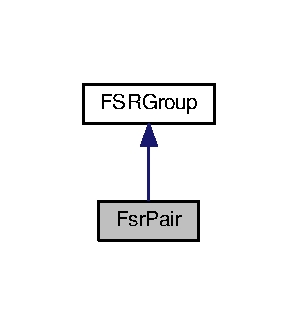
\includegraphics[width=143pt]{classFsrPair__inherit__graph}
\end{center}
\end{figure}


Collaboration diagram for Fsr\+Pair\+:
\nopagebreak
\begin{figure}[H]
\begin{center}
\leavevmode
\includegraphics[width=186pt]{classFsrPair__coll__graph}
\end{center}
\end{figure}
\subsection*{Public Member Functions}
\begin{DoxyCompactItemize}
\item 
\hyperlink{classFsrPair_a03604af09cabd102d6151610af1ef022}{Fsr\+Pair} (\hyperlink{classLinkedList}{Linked\+List}$<$ \hyperlink{classFSR}{F\+SR} $\ast$ $>$ $\ast$\hyperlink{classFSRGroup_a818ff1c99f2f1aaa5bd36c6cb701b491}{fsrs})
\item 
double \hyperlink{classFsrPair_a002d89d018c91b4e415381a444b30689}{get\+Ratio} ()
\item 
double \hyperlink{classFsrPair_aecd1acaffcf8a0c3ab60d1ddd2ac52bc}{get\+Difference} ()
\end{DoxyCompactItemize}
\subsection*{Additional Inherited Members}


\subsection{Constructor \& Destructor Documentation}
\index{Fsr\+Pair@{Fsr\+Pair}!Fsr\+Pair@{Fsr\+Pair}}
\index{Fsr\+Pair@{Fsr\+Pair}!Fsr\+Pair@{Fsr\+Pair}}
\subsubsection[{\texorpdfstring{Fsr\+Pair(\+Linked\+List$<$ F\+S\+R $\ast$ $>$ $\ast$fsrs)}{FsrPair(LinkedList< FSR * > *fsrs)}}]{\setlength{\rightskip}{0pt plus 5cm}Fsr\+Pair\+::\+Fsr\+Pair (
\begin{DoxyParamCaption}
\item[{{\bf Linked\+List}$<$ {\bf F\+SR} $\ast$ $>$ $\ast$}]{fsrs}
\end{DoxyParamCaption}
)}\hypertarget{classFsrPair_a03604af09cabd102d6151610af1ef022}{}\label{classFsrPair_a03604af09cabd102d6151610af1ef022}


\subsection{Member Function Documentation}
\index{Fsr\+Pair@{Fsr\+Pair}!get\+Difference@{get\+Difference}}
\index{get\+Difference@{get\+Difference}!Fsr\+Pair@{Fsr\+Pair}}
\subsubsection[{\texorpdfstring{get\+Difference()}{getDifference()}}]{\setlength{\rightskip}{0pt plus 5cm}double Fsr\+Pair\+::get\+Difference (
\begin{DoxyParamCaption}
{}
\end{DoxyParamCaption}
)\hspace{0.3cm}{\ttfamily [virtual]}}\hypertarget{classFsrPair_aecd1acaffcf8a0c3ab60d1ddd2ac52bc}{}\label{classFsrPair_aecd1acaffcf8a0c3ab60d1ddd2ac52bc}


Reimplemented from \hyperlink{classFSRGroup_ab12866c42645b5d892a1d69fb7056e4f}{F\+S\+R\+Group}.

\index{Fsr\+Pair@{Fsr\+Pair}!get\+Ratio@{get\+Ratio}}
\index{get\+Ratio@{get\+Ratio}!Fsr\+Pair@{Fsr\+Pair}}
\subsubsection[{\texorpdfstring{get\+Ratio()}{getRatio()}}]{\setlength{\rightskip}{0pt plus 5cm}double Fsr\+Pair\+::get\+Ratio (
\begin{DoxyParamCaption}
{}
\end{DoxyParamCaption}
)\hspace{0.3cm}{\ttfamily [virtual]}}\hypertarget{classFsrPair_a002d89d018c91b4e415381a444b30689}{}\label{classFsrPair_a002d89d018c91b4e415381a444b30689}


Reimplemented from \hyperlink{classFSRGroup_ae1658e0276de8cf7d9a3c29c84257d3b}{F\+S\+R\+Group}.



The documentation for this class was generated from the following files\+:\begin{DoxyCompactItemize}
\item 
\hyperlink{FSR_8hpp}{F\+S\+R.\+hpp}\item 
\hyperlink{FSR_8cpp}{F\+S\+R.\+cpp}\end{DoxyCompactItemize}

\hypertarget{classFSRReport}{}\section{F\+S\+R\+Report Class Reference}
\label{classFSRReport}\index{F\+S\+R\+Report@{F\+S\+R\+Report}}


{\ttfamily \#include $<$Report.\+hpp$>$}



Inheritance diagram for F\+S\+R\+Report\+:\nopagebreak
\begin{figure}[H]
\begin{center}
\leavevmode
\includegraphics[width=146pt]{classFSRReport__inherit__graph}
\end{center}
\end{figure}


Collaboration diagram for F\+S\+R\+Report\+:\nopagebreak
\begin{figure}[H]
\begin{center}
\leavevmode
\includegraphics[width=266pt]{classFSRReport__coll__graph}
\end{center}
\end{figure}
\subsection*{Public Attributes}
\begin{DoxyCompactItemize}
\item 
double \hyperlink{classFSRReport_a9373db6d07f9794282e1a56d9c605201}{threshold}
\item 
double \hyperlink{classFSRReport_a512ecbc199081bf26fe9ca185843abf2}{measured\+Force}
\end{DoxyCompactItemize}
\subsection*{Additional Inherited Members}


\subsection{Member Data Documentation}
\index{F\+S\+R\+Report@{F\+S\+R\+Report}!measured\+Force@{measured\+Force}}
\index{measured\+Force@{measured\+Force}!F\+S\+R\+Report@{F\+S\+R\+Report}}
\subsubsection[{\texorpdfstring{measured\+Force}{measuredForce}}]{\setlength{\rightskip}{0pt plus 5cm}double F\+S\+R\+Report\+::measured\+Force}\hypertarget{classFSRReport_a512ecbc199081bf26fe9ca185843abf2}{}\label{classFSRReport_a512ecbc199081bf26fe9ca185843abf2}
\index{F\+S\+R\+Report@{F\+S\+R\+Report}!threshold@{threshold}}
\index{threshold@{threshold}!F\+S\+R\+Report@{F\+S\+R\+Report}}
\subsubsection[{\texorpdfstring{threshold}{threshold}}]{\setlength{\rightskip}{0pt plus 5cm}double F\+S\+R\+Report\+::threshold}\hypertarget{classFSRReport_a9373db6d07f9794282e1a56d9c605201}{}\label{classFSRReport_a9373db6d07f9794282e1a56d9c605201}


The documentation for this class was generated from the following file\+:\begin{DoxyCompactItemize}
\item 
\hyperlink{Report_8hpp}{Report.\+hpp}\end{DoxyCompactItemize}

\hypertarget{classFSRType10}{}\section{F\+S\+R\+Type10 Class Reference}
\label{classFSRType10}\index{F\+S\+R\+Type10@{F\+S\+R\+Type10}}


{\ttfamily \#include $<$F\+S\+R.\+hpp$>$}



Inheritance diagram for F\+S\+R\+Type10\+:\nopagebreak
\begin{figure}[H]
\begin{center}
\leavevmode
\includegraphics[width=149pt]{classFSRType10__inherit__graph}
\end{center}
\end{figure}


Collaboration diagram for F\+S\+R\+Type10\+:
\nopagebreak
\begin{figure}[H]
\begin{center}
\leavevmode
\includegraphics[width=149pt]{classFSRType10__coll__graph}
\end{center}
\end{figure}
\subsection*{Public Member Functions}
\begin{DoxyCompactItemize}
\item 
\hyperlink{classFSRType10_a5dc8827b67fa988ac148dc0e7fc8c69a}{F\+S\+R\+Type10} (\hyperlink{classInputPort}{Input\+Port} $\ast$port)
\end{DoxyCompactItemize}


\subsection{Constructor \& Destructor Documentation}
\index{F\+S\+R\+Type10@{F\+S\+R\+Type10}!F\+S\+R\+Type10@{F\+S\+R\+Type10}}
\index{F\+S\+R\+Type10@{F\+S\+R\+Type10}!F\+S\+R\+Type10@{F\+S\+R\+Type10}}
\subsubsection[{\texorpdfstring{F\+S\+R\+Type10(\+Input\+Port $\ast$port)}{FSRType10(InputPort *port)}}]{\setlength{\rightskip}{0pt plus 5cm}F\+S\+R\+Type10\+::\+F\+S\+R\+Type10 (
\begin{DoxyParamCaption}
\item[{{\bf Input\+Port} $\ast$}]{port}
\end{DoxyParamCaption}
)}\hypertarget{classFSRType10_a5dc8827b67fa988ac148dc0e7fc8c69a}{}\label{classFSRType10_a5dc8827b67fa988ac148dc0e7fc8c69a}


The documentation for this class was generated from the following files\+:\begin{DoxyCompactItemize}
\item 
\hyperlink{FSR_8hpp}{F\+S\+R.\+hpp}\item 
\hyperlink{FSR_8cpp}{F\+S\+R.\+cpp}\end{DoxyCompactItemize}

\hypertarget{classFSRType40}{}\section{F\+S\+R\+Type40 Class Reference}
\label{classFSRType40}\index{F\+S\+R\+Type40@{F\+S\+R\+Type40}}


{\ttfamily \#include $<$F\+S\+R.\+hpp$>$}



Inheritance diagram for F\+S\+R\+Type40\+:\nopagebreak
\begin{figure}[H]
\begin{center}
\leavevmode
\includegraphics[width=149pt]{classFSRType40__inherit__graph}
\end{center}
\end{figure}


Collaboration diagram for F\+S\+R\+Type40\+:
\nopagebreak
\begin{figure}[H]
\begin{center}
\leavevmode
\includegraphics[width=149pt]{classFSRType40__coll__graph}
\end{center}
\end{figure}
\subsection*{Public Member Functions}
\begin{DoxyCompactItemize}
\item 
\hyperlink{classFSRType40_acacbd300e85e6dd0cfa4900477e079c6}{F\+S\+R\+Type40} (\hyperlink{classInputPort}{Input\+Port} $\ast$port)
\end{DoxyCompactItemize}


\subsection{Constructor \& Destructor Documentation}
\index{F\+S\+R\+Type40@{F\+S\+R\+Type40}!F\+S\+R\+Type40@{F\+S\+R\+Type40}}
\index{F\+S\+R\+Type40@{F\+S\+R\+Type40}!F\+S\+R\+Type40@{F\+S\+R\+Type40}}
\subsubsection[{\texorpdfstring{F\+S\+R\+Type40(\+Input\+Port $\ast$port)}{FSRType40(InputPort *port)}}]{\setlength{\rightskip}{0pt plus 5cm}F\+S\+R\+Type40\+::\+F\+S\+R\+Type40 (
\begin{DoxyParamCaption}
\item[{{\bf Input\+Port} $\ast$}]{port}
\end{DoxyParamCaption}
)}\hypertarget{classFSRType40_acacbd300e85e6dd0cfa4900477e079c6}{}\label{classFSRType40_acacbd300e85e6dd0cfa4900477e079c6}


The documentation for this class was generated from the following files\+:\begin{DoxyCompactItemize}
\item 
\hyperlink{FSR_8hpp}{F\+S\+R.\+hpp}\item 
\hyperlink{FSR_8cpp}{F\+S\+R.\+cpp}\end{DoxyCompactItemize}

\hypertarget{classGetFsrThresholdTransmission}{}\section{Get\+Fsr\+Threshold\+Transmission Class Reference}
\label{classGetFsrThresholdTransmission}\index{Get\+Fsr\+Threshold\+Transmission@{Get\+Fsr\+Threshold\+Transmission}}


{\ttfamily \#include $<$Transmission.\+hpp$>$}



Inheritance diagram for Get\+Fsr\+Threshold\+Transmission\+:\nopagebreak
\begin{figure}[H]
\begin{center}
\leavevmode
\includegraphics[width=228pt]{classGetFsrThresholdTransmission__inherit__graph}
\end{center}
\end{figure}


Collaboration diagram for Get\+Fsr\+Threshold\+Transmission\+:\nopagebreak
\begin{figure}[H]
\begin{center}
\leavevmode
\includegraphics[width=350pt]{classGetFsrThresholdTransmission__coll__graph}
\end{center}
\end{figure}
\subsection*{Public Member Functions}
\begin{DoxyCompactItemize}
\item 
\hyperlink{classGetFsrThresholdTransmission_a009e3d759e692de2ee87c52d89cce553}{Get\+Fsr\+Threshold\+Transmission} (\hyperlink{classTransceiver}{Transceiver} $\ast$\hyperlink{classTransmission_a4136f9d979a928565232a2d3d6eb5ac5}{transceiver}, \hyperlink{classCommandFactory}{Command\+Factory} $\ast$cmd)
\end{DoxyCompactItemize}
\subsection*{Additional Inherited Members}


\subsection{Constructor \& Destructor Documentation}
\index{Get\+Fsr\+Threshold\+Transmission@{Get\+Fsr\+Threshold\+Transmission}!Get\+Fsr\+Threshold\+Transmission@{Get\+Fsr\+Threshold\+Transmission}}
\index{Get\+Fsr\+Threshold\+Transmission@{Get\+Fsr\+Threshold\+Transmission}!Get\+Fsr\+Threshold\+Transmission@{Get\+Fsr\+Threshold\+Transmission}}
\subsubsection[{\texorpdfstring{Get\+Fsr\+Threshold\+Transmission(\+Transceiver $\ast$transceiver, Command\+Factory $\ast$cmd)}{GetFsrThresholdTransmission(Transceiver *transceiver, CommandFactory *cmd)}}]{\setlength{\rightskip}{0pt plus 5cm}Get\+Fsr\+Threshold\+Transmission\+::\+Get\+Fsr\+Threshold\+Transmission (
\begin{DoxyParamCaption}
\item[{{\bf Transceiver} $\ast$}]{transceiver, }
\item[{{\bf Command\+Factory} $\ast$}]{cmd}
\end{DoxyParamCaption}
)\hspace{0.3cm}{\ttfamily [explicit]}}\hypertarget{classGetFsrThresholdTransmission_a009e3d759e692de2ee87c52d89cce553}{}\label{classGetFsrThresholdTransmission_a009e3d759e692de2ee87c52d89cce553}


The documentation for this class was generated from the following files\+:\begin{DoxyCompactItemize}
\item 
\hyperlink{Transmission_8hpp}{Transmission.\+hpp}\item 
\hyperlink{Transmission_8cpp}{Transmission.\+cpp}\end{DoxyCompactItemize}

\hypertarget{classGetKFTransmission}{}\section{Get\+K\+F\+Transmission Class Reference}
\label{classGetKFTransmission}\index{Get\+K\+F\+Transmission@{Get\+K\+F\+Transmission}}


{\ttfamily \#include $<$Transmission.\+hpp$>$}



Inheritance diagram for Get\+K\+F\+Transmission\+:\nopagebreak
\begin{figure}[H]
\begin{center}
\leavevmode
\includegraphics[width=204pt]{classGetKFTransmission__inherit__graph}
\end{center}
\end{figure}


Collaboration diagram for Get\+K\+F\+Transmission\+:
\nopagebreak
\begin{figure}[H]
\begin{center}
\leavevmode
\includegraphics[width=350pt]{classGetKFTransmission__coll__graph}
\end{center}
\end{figure}
\subsection*{Public Member Functions}
\begin{DoxyCompactItemize}
\item 
\hyperlink{classGetKFTransmission_a28c781f9c8926ea016a86b8728cc187e}{Get\+K\+F\+Transmission} (\hyperlink{classTransceiver}{Transceiver} $\ast$\hyperlink{classTransmission_a4136f9d979a928565232a2d3d6eb5ac5}{transceiver}, \hyperlink{classCommandFactory}{Command\+Factory} $\ast$cmd)
\end{DoxyCompactItemize}
\subsection*{Additional Inherited Members}


\subsection{Constructor \& Destructor Documentation}
\index{Get\+K\+F\+Transmission@{Get\+K\+F\+Transmission}!Get\+K\+F\+Transmission@{Get\+K\+F\+Transmission}}
\index{Get\+K\+F\+Transmission@{Get\+K\+F\+Transmission}!Get\+K\+F\+Transmission@{Get\+K\+F\+Transmission}}
\subsubsection[{\texorpdfstring{Get\+K\+F\+Transmission(\+Transceiver $\ast$transceiver, Command\+Factory $\ast$cmd)}{GetKFTransmission(Transceiver *transceiver, CommandFactory *cmd)}}]{\setlength{\rightskip}{0pt plus 5cm}Get\+K\+F\+Transmission\+::\+Get\+K\+F\+Transmission (
\begin{DoxyParamCaption}
\item[{{\bf Transceiver} $\ast$}]{transceiver, }
\item[{{\bf Command\+Factory} $\ast$}]{cmd}
\end{DoxyParamCaption}
)\hspace{0.3cm}{\ttfamily [explicit]}}\hypertarget{classGetKFTransmission_a28c781f9c8926ea016a86b8728cc187e}{}\label{classGetKFTransmission_a28c781f9c8926ea016a86b8728cc187e}


The documentation for this class was generated from the following files\+:\begin{DoxyCompactItemize}
\item 
\hyperlink{Transmission_8hpp}{Transmission.\+hpp}\item 
\hyperlink{Transmission_8cpp}{Transmission.\+cpp}\end{DoxyCompactItemize}

\hypertarget{classGetPidParamsTransmission}{}\section{Get\+Pid\+Params\+Transmission Class Reference}
\label{classGetPidParamsTransmission}\index{Get\+Pid\+Params\+Transmission@{Get\+Pid\+Params\+Transmission}}


{\ttfamily \#include $<$Transmission.\+hpp$>$}



Inheritance diagram for Get\+Pid\+Params\+Transmission\+:\nopagebreak
\begin{figure}[H]
\begin{center}
\leavevmode
\includegraphics[width=219pt]{classGetPidParamsTransmission__inherit__graph}
\end{center}
\end{figure}


Collaboration diagram for Get\+Pid\+Params\+Transmission\+:
\nopagebreak
\begin{figure}[H]
\begin{center}
\leavevmode
\includegraphics[width=350pt]{classGetPidParamsTransmission__coll__graph}
\end{center}
\end{figure}
\subsection*{Public Member Functions}
\begin{DoxyCompactItemize}
\item 
\hyperlink{classGetPidParamsTransmission_a73c4286312024009abf888f32f639bb7}{Get\+Pid\+Params\+Transmission} (\hyperlink{classTransceiver}{Transceiver} $\ast$\hyperlink{classTransmission_a4136f9d979a928565232a2d3d6eb5ac5}{transceiver}, \hyperlink{classCommandFactory}{Command\+Factory} $\ast$cmd)
\end{DoxyCompactItemize}
\subsection*{Additional Inherited Members}


\subsection{Constructor \& Destructor Documentation}
\index{Get\+Pid\+Params\+Transmission@{Get\+Pid\+Params\+Transmission}!Get\+Pid\+Params\+Transmission@{Get\+Pid\+Params\+Transmission}}
\index{Get\+Pid\+Params\+Transmission@{Get\+Pid\+Params\+Transmission}!Get\+Pid\+Params\+Transmission@{Get\+Pid\+Params\+Transmission}}
\subsubsection[{\texorpdfstring{Get\+Pid\+Params\+Transmission(\+Transceiver $\ast$transceiver, Command\+Factory $\ast$cmd)}{GetPidParamsTransmission(Transceiver *transceiver, CommandFactory *cmd)}}]{\setlength{\rightskip}{0pt plus 5cm}Get\+Pid\+Params\+Transmission\+::\+Get\+Pid\+Params\+Transmission (
\begin{DoxyParamCaption}
\item[{{\bf Transceiver} $\ast$}]{transceiver, }
\item[{{\bf Command\+Factory} $\ast$}]{cmd}
\end{DoxyParamCaption}
)\hspace{0.3cm}{\ttfamily [explicit]}}\hypertarget{classGetPidParamsTransmission_a73c4286312024009abf888f32f639bb7}{}\label{classGetPidParamsTransmission_a73c4286312024009abf888f32f639bb7}


The documentation for this class was generated from the following files\+:\begin{DoxyCompactItemize}
\item 
\hyperlink{Transmission_8hpp}{Transmission.\+hpp}\item 
\hyperlink{Transmission_8cpp}{Transmission.\+cpp}\end{DoxyCompactItemize}

\hypertarget{classGetSetpointTransmission}{}\section{Get\+Setpoint\+Transmission Class Reference}
\label{classGetSetpointTransmission}\index{Get\+Setpoint\+Transmission@{Get\+Setpoint\+Transmission}}


{\ttfamily \#include $<$Transmission.\+hpp$>$}



Inheritance diagram for Get\+Setpoint\+Transmission\+:\nopagebreak
\begin{figure}[H]
\begin{center}
\leavevmode
\includegraphics[width=207pt]{classGetSetpointTransmission__inherit__graph}
\end{center}
\end{figure}


Collaboration diagram for Get\+Setpoint\+Transmission\+:
\nopagebreak
\begin{figure}[H]
\begin{center}
\leavevmode
\includegraphics[width=350pt]{classGetSetpointTransmission__coll__graph}
\end{center}
\end{figure}
\subsection*{Public Member Functions}
\begin{DoxyCompactItemize}
\item 
\hyperlink{classGetSetpointTransmission_aa5ee0806f221fde7789f38db020f40fd}{Get\+Setpoint\+Transmission} (\hyperlink{classTransceiver}{Transceiver} $\ast$\hyperlink{classTransmission_a4136f9d979a928565232a2d3d6eb5ac5}{transceiver}, \hyperlink{classCommandFactory}{Command\+Factory} $\ast$cmd)
\end{DoxyCompactItemize}
\subsection*{Additional Inherited Members}


\subsection{Constructor \& Destructor Documentation}
\index{Get\+Setpoint\+Transmission@{Get\+Setpoint\+Transmission}!Get\+Setpoint\+Transmission@{Get\+Setpoint\+Transmission}}
\index{Get\+Setpoint\+Transmission@{Get\+Setpoint\+Transmission}!Get\+Setpoint\+Transmission@{Get\+Setpoint\+Transmission}}
\subsubsection[{\texorpdfstring{Get\+Setpoint\+Transmission(\+Transceiver $\ast$transceiver, Command\+Factory $\ast$cmd)}{GetSetpointTransmission(Transceiver *transceiver, CommandFactory *cmd)}}]{\setlength{\rightskip}{0pt plus 5cm}Get\+Setpoint\+Transmission\+::\+Get\+Setpoint\+Transmission (
\begin{DoxyParamCaption}
\item[{{\bf Transceiver} $\ast$}]{transceiver, }
\item[{{\bf Command\+Factory} $\ast$}]{cmd}
\end{DoxyParamCaption}
)\hspace{0.3cm}{\ttfamily [explicit]}}\hypertarget{classGetSetpointTransmission_aa5ee0806f221fde7789f38db020f40fd}{}\label{classGetSetpointTransmission_aa5ee0806f221fde7789f38db020f40fd}


The documentation for this class was generated from the following files\+:\begin{DoxyCompactItemize}
\item 
\hyperlink{Transmission_8hpp}{Transmission.\+hpp}\item 
\hyperlink{Transmission_8cpp}{Transmission.\+cpp}\end{DoxyCompactItemize}

\hypertarget{classGetSmoothingParamsTransmission}{}\section{Get\+Smoothing\+Params\+Transmission Class Reference}
\label{classGetSmoothingParamsTransmission}\index{Get\+Smoothing\+Params\+Transmission@{Get\+Smoothing\+Params\+Transmission}}


{\ttfamily \#include $<$Transmission.\+hpp$>$}



Inheritance diagram for Get\+Smoothing\+Params\+Transmission\+:\nopagebreak
\begin{figure}[H]
\begin{center}
\leavevmode
\includegraphics[width=251pt]{classGetSmoothingParamsTransmission__inherit__graph}
\end{center}
\end{figure}


Collaboration diagram for Get\+Smoothing\+Params\+Transmission\+:
\nopagebreak
\begin{figure}[H]
\begin{center}
\leavevmode
\includegraphics[width=350pt]{classGetSmoothingParamsTransmission__coll__graph}
\end{center}
\end{figure}
\subsection*{Public Member Functions}
\begin{DoxyCompactItemize}
\item 
\hyperlink{classGetSmoothingParamsTransmission_a9b3a1c978fff8f13bb0aba3f326a1ba3}{Get\+Smoothing\+Params\+Transmission} (\hyperlink{classTransceiver}{Transceiver} $\ast$\hyperlink{classTransmission_a4136f9d979a928565232a2d3d6eb5ac5}{transceiver}, \hyperlink{classCommandFactory}{Command\+Factory} $\ast$cmd)
\end{DoxyCompactItemize}
\subsection*{Additional Inherited Members}


\subsection{Constructor \& Destructor Documentation}
\index{Get\+Smoothing\+Params\+Transmission@{Get\+Smoothing\+Params\+Transmission}!Get\+Smoothing\+Params\+Transmission@{Get\+Smoothing\+Params\+Transmission}}
\index{Get\+Smoothing\+Params\+Transmission@{Get\+Smoothing\+Params\+Transmission}!Get\+Smoothing\+Params\+Transmission@{Get\+Smoothing\+Params\+Transmission}}
\subsubsection[{\texorpdfstring{Get\+Smoothing\+Params\+Transmission(\+Transceiver $\ast$transceiver, Command\+Factory $\ast$cmd)}{GetSmoothingParamsTransmission(Transceiver *transceiver, CommandFactory *cmd)}}]{\setlength{\rightskip}{0pt plus 5cm}Get\+Smoothing\+Params\+Transmission\+::\+Get\+Smoothing\+Params\+Transmission (
\begin{DoxyParamCaption}
\item[{{\bf Transceiver} $\ast$}]{transceiver, }
\item[{{\bf Command\+Factory} $\ast$}]{cmd}
\end{DoxyParamCaption}
)\hspace{0.3cm}{\ttfamily [explicit]}}\hypertarget{classGetSmoothingParamsTransmission_a9b3a1c978fff8f13bb0aba3f326a1ba3}{}\label{classGetSmoothingParamsTransmission_a9b3a1c978fff8f13bb0aba3f326a1ba3}


The documentation for this class was generated from the following files\+:\begin{DoxyCompactItemize}
\item 
\hyperlink{Transmission_8hpp}{Transmission.\+hpp}\item 
\hyperlink{Transmission_8cpp}{Transmission.\+cpp}\end{DoxyCompactItemize}

\hypertarget{classIMU}{}\section{I\+MU Class Reference}
\label{classIMU}\index{I\+MU@{I\+MU}}


{\ttfamily \#include $<$I\+M\+U.\+hpp$>$}

\subsection*{Public Member Functions}
\begin{DoxyCompactItemize}
\item 
\hyperlink{classIMU_aaf1bd21ea92633767b28a34b65cbfb80}{I\+MU} (\hyperlink{classImuPort}{Imu\+Port} $\ast$imu\+\_\+port, unsigned int address)
\item 
\hyperlink{classIMU_ad1f213d1e6aa08988ff683feab721559}{$\sim$\+I\+MU} ()
\item 
void \hyperlink{classIMU_a2be1f7017e9a8747790ffd4a0d116f4c}{calibrate} ()
\item 
void \hyperlink{classIMU_a8f433c96a79fce2a0bac01cd1376fca8}{measure} ()
\item 
void \hyperlink{classIMU_ae14f358bcda39a1dc54fa932417adcd1}{get\+Orientation} (double $\ast$orientation)
\item 
\hyperlink{classIMUReport}{I\+M\+U\+Report} $\ast$ \hyperlink{classIMU_a5a56602778602302d4b4b2f79e25bb87}{generate\+Report} ()
\item 
void \hyperlink{classIMU_a5fabb3089472bdf2d697c3487893a031}{fill\+Report} (\hyperlink{classIMUReport}{I\+M\+U\+Report} $\ast$report)
\item 
void \hyperlink{classIMU_ac3e9fe8145cddc7b0fee67df0f097f22}{fill\+Local\+Report} (\hyperlink{classIMUReport}{I\+M\+U\+Report} $\ast$report)
\end{DoxyCompactItemize}


\subsection{Constructor \& Destructor Documentation}
\index{I\+MU@{I\+MU}!I\+MU@{I\+MU}}
\index{I\+MU@{I\+MU}!I\+MU@{I\+MU}}
\subsubsection[{\texorpdfstring{I\+M\+U(\+Imu\+Port $\ast$imu\+\_\+port, unsigned int address)}{IMU(ImuPort *imu_port, unsigned int address)}}]{\setlength{\rightskip}{0pt plus 5cm}I\+M\+U\+::\+I\+MU (
\begin{DoxyParamCaption}
\item[{{\bf Imu\+Port} $\ast$}]{imu\+\_\+port, }
\item[{unsigned int}]{address}
\end{DoxyParamCaption}
)}\hypertarget{classIMU_aaf1bd21ea92633767b28a34b65cbfb80}{}\label{classIMU_aaf1bd21ea92633767b28a34b65cbfb80}
\index{I\+MU@{I\+MU}!````~I\+MU@{$\sim$\+I\+MU}}
\index{````~I\+MU@{$\sim$\+I\+MU}!I\+MU@{I\+MU}}
\subsubsection[{\texorpdfstring{$\sim$\+I\+M\+U()}{~IMU()}}]{\setlength{\rightskip}{0pt plus 5cm}I\+M\+U\+::$\sim$\+I\+MU (
\begin{DoxyParamCaption}
{}
\end{DoxyParamCaption}
)}\hypertarget{classIMU_ad1f213d1e6aa08988ff683feab721559}{}\label{classIMU_ad1f213d1e6aa08988ff683feab721559}


\subsection{Member Function Documentation}
\index{I\+MU@{I\+MU}!calibrate@{calibrate}}
\index{calibrate@{calibrate}!I\+MU@{I\+MU}}
\subsubsection[{\texorpdfstring{calibrate()}{calibrate()}}]{\setlength{\rightskip}{0pt plus 5cm}void I\+M\+U\+::calibrate (
\begin{DoxyParamCaption}
{}
\end{DoxyParamCaption}
)}\hypertarget{classIMU_a2be1f7017e9a8747790ffd4a0d116f4c}{}\label{classIMU_a2be1f7017e9a8747790ffd4a0d116f4c}
\index{I\+MU@{I\+MU}!fill\+Local\+Report@{fill\+Local\+Report}}
\index{fill\+Local\+Report@{fill\+Local\+Report}!I\+MU@{I\+MU}}
\subsubsection[{\texorpdfstring{fill\+Local\+Report(\+I\+M\+U\+Report $\ast$report)}{fillLocalReport(IMUReport *report)}}]{\setlength{\rightskip}{0pt plus 5cm}void I\+M\+U\+::fill\+Local\+Report (
\begin{DoxyParamCaption}
\item[{{\bf I\+M\+U\+Report} $\ast$}]{report}
\end{DoxyParamCaption}
)}\hypertarget{classIMU_ac3e9fe8145cddc7b0fee67df0f097f22}{}\label{classIMU_ac3e9fe8145cddc7b0fee67df0f097f22}
\index{I\+MU@{I\+MU}!fill\+Report@{fill\+Report}}
\index{fill\+Report@{fill\+Report}!I\+MU@{I\+MU}}
\subsubsection[{\texorpdfstring{fill\+Report(\+I\+M\+U\+Report $\ast$report)}{fillReport(IMUReport *report)}}]{\setlength{\rightskip}{0pt plus 5cm}void I\+M\+U\+::fill\+Report (
\begin{DoxyParamCaption}
\item[{{\bf I\+M\+U\+Report} $\ast$}]{report}
\end{DoxyParamCaption}
)}\hypertarget{classIMU_a5fabb3089472bdf2d697c3487893a031}{}\label{classIMU_a5fabb3089472bdf2d697c3487893a031}
\index{I\+MU@{I\+MU}!generate\+Report@{generate\+Report}}
\index{generate\+Report@{generate\+Report}!I\+MU@{I\+MU}}
\subsubsection[{\texorpdfstring{generate\+Report()}{generateReport()}}]{\setlength{\rightskip}{0pt plus 5cm}{\bf I\+M\+U\+Report} $\ast$ I\+M\+U\+::generate\+Report (
\begin{DoxyParamCaption}
{}
\end{DoxyParamCaption}
)}\hypertarget{classIMU_a5a56602778602302d4b4b2f79e25bb87}{}\label{classIMU_a5a56602778602302d4b4b2f79e25bb87}
\index{I\+MU@{I\+MU}!get\+Orientation@{get\+Orientation}}
\index{get\+Orientation@{get\+Orientation}!I\+MU@{I\+MU}}
\subsubsection[{\texorpdfstring{get\+Orientation(double $\ast$orientation)}{getOrientation(double *orientation)}}]{\setlength{\rightskip}{0pt plus 5cm}void I\+M\+U\+::get\+Orientation (
\begin{DoxyParamCaption}
\item[{double $\ast$}]{orientation}
\end{DoxyParamCaption}
)}\hypertarget{classIMU_ae14f358bcda39a1dc54fa932417adcd1}{}\label{classIMU_ae14f358bcda39a1dc54fa932417adcd1}
\index{I\+MU@{I\+MU}!measure@{measure}}
\index{measure@{measure}!I\+MU@{I\+MU}}
\subsubsection[{\texorpdfstring{measure()}{measure()}}]{\setlength{\rightskip}{0pt plus 5cm}void I\+M\+U\+::measure (
\begin{DoxyParamCaption}
{}
\end{DoxyParamCaption}
)}\hypertarget{classIMU_a8f433c96a79fce2a0bac01cd1376fca8}{}\label{classIMU_a8f433c96a79fce2a0bac01cd1376fca8}


The documentation for this class was generated from the following files\+:\begin{DoxyCompactItemize}
\item 
\hyperlink{IMU_8hpp}{I\+M\+U.\+hpp}\item 
\hyperlink{IMU_8cpp}{I\+M\+U.\+cpp}\end{DoxyCompactItemize}

\hypertarget{classImuPort}{}\section{Imu\+Port Class Reference}
\label{classImuPort}\index{Imu\+Port@{Imu\+Port}}


{\ttfamily \#include $<$Port.\+hpp$>$}



Inheritance diagram for Imu\+Port\+:\nopagebreak
\begin{figure}[H]
\begin{center}
\leavevmode
\includegraphics[width=131pt]{classImuPort__inherit__graph}
\end{center}
\end{figure}


Collaboration diagram for Imu\+Port\+:\nopagebreak
\begin{figure}[H]
\begin{center}
\leavevmode
\includegraphics[width=131pt]{classImuPort__coll__graph}
\end{center}
\end{figure}
\subsection*{Public Member Functions}
\begin{DoxyCompactItemize}
\item 
\hyperlink{classImuPort_a5fd86378f772f9eedf0d125229fc9bc0}{Imu\+Port} (\hyperlink{Arduino_8hpp_aaa5bce2cb83fc43fec67214bf4feea69}{i2c\+\_\+pins} imu\+\_\+pins)
\item 
\hyperlink{Arduino_8hpp_aaa5bce2cb83fc43fec67214bf4feea69}{i2c\+\_\+pins} \hyperlink{classImuPort_a16c0e671ec33d7533130b0c1af51a216}{get\+Pins} ()
\item 
\hyperlink{Arduino_8hpp_ab2e3db7382e551f5b0485447adcad03e}{i2c\+\_\+bus} \hyperlink{classImuPort_aecbe963045ee71d96a4fccfe27537e51}{get\+Bus} ()
\item 
virtual \hyperlink{classImuPort_acc89c78df2ebb97834f035a97435ac5a}{$\sim$\+Imu\+Port} ()
\end{DoxyCompactItemize}
\subsection*{Additional Inherited Members}


\subsection{Constructor \& Destructor Documentation}
\index{Imu\+Port@{Imu\+Port}!Imu\+Port@{Imu\+Port}}
\index{Imu\+Port@{Imu\+Port}!Imu\+Port@{Imu\+Port}}
\subsubsection[{\texorpdfstring{Imu\+Port(i2c\+\_\+pins imu\+\_\+pins)}{ImuPort(i2c_pins imu_pins)}}]{\setlength{\rightskip}{0pt plus 5cm}Imu\+Port\+::\+Imu\+Port (
\begin{DoxyParamCaption}
\item[{{\bf i2c\+\_\+pins}}]{imu\+\_\+pins}
\end{DoxyParamCaption}
)}\hypertarget{classImuPort_a5fd86378f772f9eedf0d125229fc9bc0}{}\label{classImuPort_a5fd86378f772f9eedf0d125229fc9bc0}
\index{Imu\+Port@{Imu\+Port}!````~Imu\+Port@{$\sim$\+Imu\+Port}}
\index{````~Imu\+Port@{$\sim$\+Imu\+Port}!Imu\+Port@{Imu\+Port}}
\subsubsection[{\texorpdfstring{$\sim$\+Imu\+Port()}{~ImuPort()}}]{\setlength{\rightskip}{0pt plus 5cm}Imu\+Port\+::$\sim$\+Imu\+Port (
\begin{DoxyParamCaption}
{}
\end{DoxyParamCaption}
)\hspace{0.3cm}{\ttfamily [virtual]}}\hypertarget{classImuPort_acc89c78df2ebb97834f035a97435ac5a}{}\label{classImuPort_acc89c78df2ebb97834f035a97435ac5a}


\subsection{Member Function Documentation}
\index{Imu\+Port@{Imu\+Port}!get\+Bus@{get\+Bus}}
\index{get\+Bus@{get\+Bus}!Imu\+Port@{Imu\+Port}}
\subsubsection[{\texorpdfstring{get\+Bus()}{getBus()}}]{\setlength{\rightskip}{0pt plus 5cm}{\bf i2c\+\_\+bus} Imu\+Port\+::get\+Bus (
\begin{DoxyParamCaption}
{}
\end{DoxyParamCaption}
)}\hypertarget{classImuPort_aecbe963045ee71d96a4fccfe27537e51}{}\label{classImuPort_aecbe963045ee71d96a4fccfe27537e51}
\index{Imu\+Port@{Imu\+Port}!get\+Pins@{get\+Pins}}
\index{get\+Pins@{get\+Pins}!Imu\+Port@{Imu\+Port}}
\subsubsection[{\texorpdfstring{get\+Pins()}{getPins()}}]{\setlength{\rightskip}{0pt plus 5cm}{\bf i2c\+\_\+pins} Imu\+Port\+::get\+Pins (
\begin{DoxyParamCaption}
{}
\end{DoxyParamCaption}
)}\hypertarget{classImuPort_a16c0e671ec33d7533130b0c1af51a216}{}\label{classImuPort_a16c0e671ec33d7533130b0c1af51a216}


The documentation for this class was generated from the following files\+:\begin{DoxyCompactItemize}
\item 
\hyperlink{Port_8hpp}{Port.\+hpp}\item 
\hyperlink{Port_8cpp}{Port.\+cpp}\end{DoxyCompactItemize}

\hypertarget{classIMUReport}{}\section{I\+M\+U\+Report Class Reference}
\label{classIMUReport}\index{I\+M\+U\+Report@{I\+M\+U\+Report}}


{\ttfamily \#include $<$Report.\+hpp$>$}



Inheritance diagram for I\+M\+U\+Report\+:\nopagebreak
\begin{figure}[H]
\begin{center}
\leavevmode
\includegraphics[width=145pt]{classIMUReport__inherit__graph}
\end{center}
\end{figure}


Collaboration diagram for I\+M\+U\+Report\+:\nopagebreak
\begin{figure}[H]
\begin{center}
\leavevmode
\includegraphics[width=266pt]{classIMUReport__coll__graph}
\end{center}
\end{figure}
\subsection*{Public Attributes}
\begin{DoxyCompactItemize}
\item 
double \hyperlink{classIMUReport_a7ec71e96725321584168465be9008387}{orientation} \mbox{[}3\mbox{]}
\end{DoxyCompactItemize}
\subsection*{Additional Inherited Members}


\subsection{Member Data Documentation}
\index{I\+M\+U\+Report@{I\+M\+U\+Report}!orientation@{orientation}}
\index{orientation@{orientation}!I\+M\+U\+Report@{I\+M\+U\+Report}}
\subsubsection[{\texorpdfstring{orientation}{orientation}}]{\setlength{\rightskip}{0pt plus 5cm}double I\+M\+U\+Report\+::orientation\mbox{[}3\mbox{]}}\hypertarget{classIMUReport_a7ec71e96725321584168465be9008387}{}\label{classIMUReport_a7ec71e96725321584168465be9008387}


The documentation for this class was generated from the following file\+:\begin{DoxyCompactItemize}
\item 
\hyperlink{Report_8hpp}{Report.\+hpp}\end{DoxyCompactItemize}

\hypertarget{classInputPort}{}\section{Input\+Port Class Reference}
\label{classInputPort}\index{Input\+Port@{Input\+Port}}


{\ttfamily \#include $<$Port.\+hpp$>$}



Inheritance diagram for Input\+Port\+:\nopagebreak
\begin{figure}[H]
\begin{center}
\leavevmode
\includegraphics[width=334pt]{classInputPort__inherit__graph}
\end{center}
\end{figure}


Collaboration diagram for Input\+Port\+:\nopagebreak
\begin{figure}[H]
\begin{center}
\leavevmode
\includegraphics[width=136pt]{classInputPort__coll__graph}
\end{center}
\end{figure}
\subsection*{Public Member Functions}
\begin{DoxyCompactItemize}
\item 
\hyperlink{classInputPort_a00c5fd37d876e4ea4c3ffc13dcd4607d}{Input\+Port} (unsigned int pin)
\item 
virtual double \hyperlink{classInputPort_a0dd029736ef41eaf5c1b079c3b8d4ba3}{read} ()=0
\item 
virtual \hyperlink{classInputPort_aa0f6e0fca872353ed17b1e53c6c04508}{$\sim$\+Input\+Port} ()
\end{DoxyCompactItemize}
\subsection*{Additional Inherited Members}


\subsection{Constructor \& Destructor Documentation}
\index{Input\+Port@{Input\+Port}!Input\+Port@{Input\+Port}}
\index{Input\+Port@{Input\+Port}!Input\+Port@{Input\+Port}}
\subsubsection[{\texorpdfstring{Input\+Port(unsigned int pin)}{InputPort(unsigned int pin)}}]{\setlength{\rightskip}{0pt plus 5cm}Input\+Port\+::\+Input\+Port (
\begin{DoxyParamCaption}
\item[{unsigned int}]{pin}
\end{DoxyParamCaption}
)}\hypertarget{classInputPort_a00c5fd37d876e4ea4c3ffc13dcd4607d}{}\label{classInputPort_a00c5fd37d876e4ea4c3ffc13dcd4607d}
\index{Input\+Port@{Input\+Port}!````~Input\+Port@{$\sim$\+Input\+Port}}
\index{````~Input\+Port@{$\sim$\+Input\+Port}!Input\+Port@{Input\+Port}}
\subsubsection[{\texorpdfstring{$\sim$\+Input\+Port()}{~InputPort()}}]{\setlength{\rightskip}{0pt plus 5cm}Input\+Port\+::$\sim$\+Input\+Port (
\begin{DoxyParamCaption}
{}
\end{DoxyParamCaption}
)\hspace{0.3cm}{\ttfamily [virtual]}}\hypertarget{classInputPort_aa0f6e0fca872353ed17b1e53c6c04508}{}\label{classInputPort_aa0f6e0fca872353ed17b1e53c6c04508}


\subsection{Member Function Documentation}
\index{Input\+Port@{Input\+Port}!read@{read}}
\index{read@{read}!Input\+Port@{Input\+Port}}
\subsubsection[{\texorpdfstring{read()=0}{read()=0}}]{\setlength{\rightskip}{0pt plus 5cm}virtual double Input\+Port\+::read (
\begin{DoxyParamCaption}
{}
\end{DoxyParamCaption}
)\hspace{0.3cm}{\ttfamily [pure virtual]}}\hypertarget{classInputPort_a0dd029736ef41eaf5c1b079c3b8d4ba3}{}\label{classInputPort_a0dd029736ef41eaf5c1b079c3b8d4ba3}


Implemented in \hyperlink{classRxPort_aadcb174266e7f5daf3afb9a30433d0a3}{Rx\+Port}, \hyperlink{classDigitalInputPort_aada74a73fe70ea59db9399e39190aa5a}{Digital\+Input\+Port}, and \hyperlink{classAnalogInputPort_a7668c7a5ff22d7e75f3ac939070b7dad}{Analog\+Input\+Port}.



The documentation for this class was generated from the following files\+:\begin{DoxyCompactItemize}
\item 
\hyperlink{Port_8hpp}{Port.\+hpp}\item 
\hyperlink{Port_8cpp}{Port.\+cpp}\end{DoxyCompactItemize}

\hypertarget{classJoint}{}\section{Joint Class Reference}
\label{classJoint}\index{Joint@{Joint}}


{\ttfamily \#include $<$Joint.\+hpp$>$}

\subsection*{Public Member Functions}
\begin{DoxyCompactItemize}
\item 
\hyperlink{classJoint_a2e5c866dcb711094af82278e4d44d8b2}{Joint} (\hyperlink{classControlModule}{Control\+Module} $\ast$controller, \hyperlink{classMotor}{Motor} $\ast$motor, \hyperlink{classTorqueSensor}{Torque\+Sensor} $\ast$torque\+\_\+sensor, \hyperlink{classPot}{Pot} $\ast$pot)
\item 
\hyperlink{classJoint_a42aca0bd1832136984923713127c28f1}{$\sim$\+Joint} ()
\item 
void \hyperlink{classJoint_a33729eeab4588211b7cbe753fb049d59}{process\+Message} (\hyperlink{classJointMessage}{Joint\+Message} $\ast$msg)
\item 
\hyperlink{classJointReport}{Joint\+Report} $\ast$ \hyperlink{classJoint_a65c605e61d6e1998d71a3580896ca523}{generate\+Report} ()
\item 
void \hyperlink{classJoint_aba8104e0e6b09058c7a744a805bbfa7f}{fill\+Report} (\hyperlink{classJointReport}{Joint\+Report} $\ast$report)
\item 
void \hyperlink{classJoint_ae1e7cbd5ec6ff5f8fd8a917b154a0a68}{set\+Desired\+Setpoint} (\hyperlink{States_8hpp_a26aafbeccd8f356b39e1809f1ab9cfdc}{State\+ID} state, double setpoint)
\item 
double \hyperlink{classJoint_a69a208e0b5e673d335c06d943534724d}{get\+Desired\+Setpoint} (\hyperlink{States_8hpp_a26aafbeccd8f356b39e1809f1ab9cfdc}{State\+ID} state)
\item 
void \hyperlink{classJoint_af9071b64d69bd951e215f0cf4af7b919}{measure\+Sensors} ()
\item 
double \hyperlink{classJoint_ae0204ef60dd8506dbdb94a65faa188fb}{get\+Angle} ()
\item 
bool \hyperlink{classJoint_a7fb5248914eb948e6addb4e1398c0819}{has\+Errored} ()
\item 
bool \hyperlink{classJoint_a47129449e8b008732e28b4bb0bc52643}{apply\+Torque} ()
\item 
void \hyperlink{classJoint_aa6964b1dec64a9c76b7a5a082f700493}{set\+To\+Zero} ()
\item 
void \hyperlink{classJoint_a29e0a32427976e087e35ea881fb58449}{reset\+Starting\+Parameters} ()
\item 
void \hyperlink{classJoint_ad39647a7d64b22dac562fa977344ecac}{adjust\+Shaping\+For\+Time} (double planter\+Time)
\item 
void \hyperlink{classJoint_abed0afe032168f8f554c78e7f82a5394}{update\+Motor\+Output} (\hyperlink{classSensorReport}{Sensor\+Report} $\ast$report)
\item 
void \hyperlink{classJoint_a6a4d31e980f795d5b951323ac5fd0626}{change\+Control} (\hyperlink{States_8hpp_a26aafbeccd8f356b39e1809f1ab9cfdc}{State\+ID} state\+\_\+id)
\item 
void \hyperlink{classJoint_a012a6a79e4ef4951f033b8bdbe49e93d}{apply\+Auto\+KF} ()
\item 
double \hyperlink{classJoint_a75111a7b8091c6ca5f0788704a7c1b1c}{get\+Torque} ()
\item 
void \hyperlink{classJoint_af1397d8f10d7e4509b14d5291d1c1d11}{set\+Sign} (int sign)
\item 
void \hyperlink{classJoint_ae6a96eb43fcdf599bf62fed7f8a09aa2}{set\+Pid} (double \hyperlink{Parameters_8hpp_ad1ae3be971981842496c18dabdd2e4c1}{p}, double i, double d)
\item 
void \hyperlink{classJoint_a1b138e33fe58097b42f43ade71bf8f17}{get\+Pid} (double $\ast$pid)
\item 
double \hyperlink{classJoint_a6dc498ec465f965d87533a34ee9b62d4}{get\+Kf} ()
\item 
void \hyperlink{classJoint_a99cbfdb591d588f8f8f018385f45a52c}{set\+Kf} (double kf)
\item 
double \hyperlink{classJoint_ac65cae6a80c68689ecc1e1c23c1f0aca}{get\+Smoothing\+Param} (\hyperlink{States_8hpp_a26aafbeccd8f356b39e1809f1ab9cfdc}{State\+ID} state)
\item 
void \hyperlink{classJoint_a582b21a00df5a1a5079b3bb8ba8e8af0}{set\+Smoothing\+Param} (\hyperlink{States_8hpp_a26aafbeccd8f356b39e1809f1ab9cfdc}{State\+ID} state, double param)
\item 
void \hyperlink{classJoint_ab8b007027b56b90bdf0488926f63ddf6}{start\+Torque\+Calibration} ()
\item 
void \hyperlink{classJoint_a393c16f6d5aad78c8447b275c46ef201}{update\+Torque\+Calibration} ()
\item 
void \hyperlink{classJoint_a4a9f131afc5991affa8e05e3928bf4d8}{end\+Torque\+Calibration} ()
\end{DoxyCompactItemize}


\subsection{Constructor \& Destructor Documentation}
\index{Joint@{Joint}!Joint@{Joint}}
\index{Joint@{Joint}!Joint@{Joint}}
\subsubsection[{\texorpdfstring{Joint(\+Control\+Module $\ast$controller, Motor $\ast$motor, Torque\+Sensor $\ast$torque\+\_\+sensor, Pot $\ast$pot)}{Joint(ControlModule *controller, Motor *motor, TorqueSensor *torque_sensor, Pot *pot)}}]{\setlength{\rightskip}{0pt plus 5cm}Joint\+::\+Joint (
\begin{DoxyParamCaption}
\item[{{\bf Control\+Module} $\ast$}]{controller, }
\item[{{\bf Motor} $\ast$}]{motor, }
\item[{{\bf Torque\+Sensor} $\ast$}]{torque\+\_\+sensor, }
\item[{{\bf Pot} $\ast$}]{pot}
\end{DoxyParamCaption}
)}\hypertarget{classJoint_a2e5c866dcb711094af82278e4d44d8b2}{}\label{classJoint_a2e5c866dcb711094af82278e4d44d8b2}
\index{Joint@{Joint}!````~Joint@{$\sim$\+Joint}}
\index{````~Joint@{$\sim$\+Joint}!Joint@{Joint}}
\subsubsection[{\texorpdfstring{$\sim$\+Joint()}{~Joint()}}]{\setlength{\rightskip}{0pt plus 5cm}Joint\+::$\sim$\+Joint (
\begin{DoxyParamCaption}
{}
\end{DoxyParamCaption}
)}\hypertarget{classJoint_a42aca0bd1832136984923713127c28f1}{}\label{classJoint_a42aca0bd1832136984923713127c28f1}


\subsection{Member Function Documentation}
\index{Joint@{Joint}!adjust\+Shaping\+For\+Time@{adjust\+Shaping\+For\+Time}}
\index{adjust\+Shaping\+For\+Time@{adjust\+Shaping\+For\+Time}!Joint@{Joint}}
\subsubsection[{\texorpdfstring{adjust\+Shaping\+For\+Time(double planter\+Time)}{adjustShapingForTime(double planterTime)}}]{\setlength{\rightskip}{0pt plus 5cm}void Joint\+::adjust\+Shaping\+For\+Time (
\begin{DoxyParamCaption}
\item[{double}]{planter\+Time}
\end{DoxyParamCaption}
)}\hypertarget{classJoint_ad39647a7d64b22dac562fa977344ecac}{}\label{classJoint_ad39647a7d64b22dac562fa977344ecac}
\index{Joint@{Joint}!apply\+Auto\+KF@{apply\+Auto\+KF}}
\index{apply\+Auto\+KF@{apply\+Auto\+KF}!Joint@{Joint}}
\subsubsection[{\texorpdfstring{apply\+Auto\+K\+F()}{applyAutoKF()}}]{\setlength{\rightskip}{0pt plus 5cm}void Joint\+::apply\+Auto\+KF (
\begin{DoxyParamCaption}
{}
\end{DoxyParamCaption}
)}\hypertarget{classJoint_a012a6a79e4ef4951f033b8bdbe49e93d}{}\label{classJoint_a012a6a79e4ef4951f033b8bdbe49e93d}
\index{Joint@{Joint}!apply\+Torque@{apply\+Torque}}
\index{apply\+Torque@{apply\+Torque}!Joint@{Joint}}
\subsubsection[{\texorpdfstring{apply\+Torque()}{applyTorque()}}]{\setlength{\rightskip}{0pt plus 5cm}bool Joint\+::apply\+Torque (
\begin{DoxyParamCaption}
{}
\end{DoxyParamCaption}
)}\hypertarget{classJoint_a47129449e8b008732e28b4bb0bc52643}{}\label{classJoint_a47129449e8b008732e28b4bb0bc52643}
\index{Joint@{Joint}!change\+Control@{change\+Control}}
\index{change\+Control@{change\+Control}!Joint@{Joint}}
\subsubsection[{\texorpdfstring{change\+Control(\+State\+I\+D state\+\_\+id)}{changeControl(StateID state_id)}}]{\setlength{\rightskip}{0pt plus 5cm}void Joint\+::change\+Control (
\begin{DoxyParamCaption}
\item[{{\bf State\+ID}}]{state\+\_\+id}
\end{DoxyParamCaption}
)}\hypertarget{classJoint_a6a4d31e980f795d5b951323ac5fd0626}{}\label{classJoint_a6a4d31e980f795d5b951323ac5fd0626}
\index{Joint@{Joint}!end\+Torque\+Calibration@{end\+Torque\+Calibration}}
\index{end\+Torque\+Calibration@{end\+Torque\+Calibration}!Joint@{Joint}}
\subsubsection[{\texorpdfstring{end\+Torque\+Calibration()}{endTorqueCalibration()}}]{\setlength{\rightskip}{0pt plus 5cm}void Joint\+::end\+Torque\+Calibration (
\begin{DoxyParamCaption}
{}
\end{DoxyParamCaption}
)}\hypertarget{classJoint_a4a9f131afc5991affa8e05e3928bf4d8}{}\label{classJoint_a4a9f131afc5991affa8e05e3928bf4d8}
\index{Joint@{Joint}!fill\+Report@{fill\+Report}}
\index{fill\+Report@{fill\+Report}!Joint@{Joint}}
\subsubsection[{\texorpdfstring{fill\+Report(\+Joint\+Report $\ast$report)}{fillReport(JointReport *report)}}]{\setlength{\rightskip}{0pt plus 5cm}void Joint\+::fill\+Report (
\begin{DoxyParamCaption}
\item[{{\bf Joint\+Report} $\ast$}]{report}
\end{DoxyParamCaption}
)}\hypertarget{classJoint_aba8104e0e6b09058c7a744a805bbfa7f}{}\label{classJoint_aba8104e0e6b09058c7a744a805bbfa7f}
\index{Joint@{Joint}!generate\+Report@{generate\+Report}}
\index{generate\+Report@{generate\+Report}!Joint@{Joint}}
\subsubsection[{\texorpdfstring{generate\+Report()}{generateReport()}}]{\setlength{\rightskip}{0pt plus 5cm}{\bf Joint\+Report} $\ast$ Joint\+::generate\+Report (
\begin{DoxyParamCaption}
{}
\end{DoxyParamCaption}
)}\hypertarget{classJoint_a65c605e61d6e1998d71a3580896ca523}{}\label{classJoint_a65c605e61d6e1998d71a3580896ca523}
\index{Joint@{Joint}!get\+Angle@{get\+Angle}}
\index{get\+Angle@{get\+Angle}!Joint@{Joint}}
\subsubsection[{\texorpdfstring{get\+Angle()}{getAngle()}}]{\setlength{\rightskip}{0pt plus 5cm}double Joint\+::get\+Angle (
\begin{DoxyParamCaption}
{}
\end{DoxyParamCaption}
)}\hypertarget{classJoint_ae0204ef60dd8506dbdb94a65faa188fb}{}\label{classJoint_ae0204ef60dd8506dbdb94a65faa188fb}
\index{Joint@{Joint}!get\+Desired\+Setpoint@{get\+Desired\+Setpoint}}
\index{get\+Desired\+Setpoint@{get\+Desired\+Setpoint}!Joint@{Joint}}
\subsubsection[{\texorpdfstring{get\+Desired\+Setpoint(\+State\+I\+D state)}{getDesiredSetpoint(StateID state)}}]{\setlength{\rightskip}{0pt plus 5cm}double Joint\+::get\+Desired\+Setpoint (
\begin{DoxyParamCaption}
\item[{{\bf State\+ID}}]{state}
\end{DoxyParamCaption}
)}\hypertarget{classJoint_a69a208e0b5e673d335c06d943534724d}{}\label{classJoint_a69a208e0b5e673d335c06d943534724d}
\index{Joint@{Joint}!get\+Kf@{get\+Kf}}
\index{get\+Kf@{get\+Kf}!Joint@{Joint}}
\subsubsection[{\texorpdfstring{get\+Kf()}{getKf()}}]{\setlength{\rightskip}{0pt plus 5cm}double Joint\+::get\+Kf (
\begin{DoxyParamCaption}
{}
\end{DoxyParamCaption}
)}\hypertarget{classJoint_a6dc498ec465f965d87533a34ee9b62d4}{}\label{classJoint_a6dc498ec465f965d87533a34ee9b62d4}
\index{Joint@{Joint}!get\+Pid@{get\+Pid}}
\index{get\+Pid@{get\+Pid}!Joint@{Joint}}
\subsubsection[{\texorpdfstring{get\+Pid(double $\ast$pid)}{getPid(double *pid)}}]{\setlength{\rightskip}{0pt plus 5cm}void Joint\+::get\+Pid (
\begin{DoxyParamCaption}
\item[{double $\ast$}]{pid}
\end{DoxyParamCaption}
)}\hypertarget{classJoint_a1b138e33fe58097b42f43ade71bf8f17}{}\label{classJoint_a1b138e33fe58097b42f43ade71bf8f17}
\index{Joint@{Joint}!get\+Smoothing\+Param@{get\+Smoothing\+Param}}
\index{get\+Smoothing\+Param@{get\+Smoothing\+Param}!Joint@{Joint}}
\subsubsection[{\texorpdfstring{get\+Smoothing\+Param(\+State\+I\+D state)}{getSmoothingParam(StateID state)}}]{\setlength{\rightskip}{0pt plus 5cm}double Joint\+::get\+Smoothing\+Param (
\begin{DoxyParamCaption}
\item[{{\bf State\+ID}}]{state}
\end{DoxyParamCaption}
)}\hypertarget{classJoint_ac65cae6a80c68689ecc1e1c23c1f0aca}{}\label{classJoint_ac65cae6a80c68689ecc1e1c23c1f0aca}
\index{Joint@{Joint}!get\+Torque@{get\+Torque}}
\index{get\+Torque@{get\+Torque}!Joint@{Joint}}
\subsubsection[{\texorpdfstring{get\+Torque()}{getTorque()}}]{\setlength{\rightskip}{0pt plus 5cm}double Joint\+::get\+Torque (
\begin{DoxyParamCaption}
{}
\end{DoxyParamCaption}
)}\hypertarget{classJoint_a75111a7b8091c6ca5f0788704a7c1b1c}{}\label{classJoint_a75111a7b8091c6ca5f0788704a7c1b1c}
\index{Joint@{Joint}!has\+Errored@{has\+Errored}}
\index{has\+Errored@{has\+Errored}!Joint@{Joint}}
\subsubsection[{\texorpdfstring{has\+Errored()}{hasErrored()}}]{\setlength{\rightskip}{0pt plus 5cm}bool Joint\+::has\+Errored (
\begin{DoxyParamCaption}
{}
\end{DoxyParamCaption}
)}\hypertarget{classJoint_a7fb5248914eb948e6addb4e1398c0819}{}\label{classJoint_a7fb5248914eb948e6addb4e1398c0819}
\index{Joint@{Joint}!measure\+Sensors@{measure\+Sensors}}
\index{measure\+Sensors@{measure\+Sensors}!Joint@{Joint}}
\subsubsection[{\texorpdfstring{measure\+Sensors()}{measureSensors()}}]{\setlength{\rightskip}{0pt plus 5cm}void Joint\+::measure\+Sensors (
\begin{DoxyParamCaption}
{}
\end{DoxyParamCaption}
)}\hypertarget{classJoint_af9071b64d69bd951e215f0cf4af7b919}{}\label{classJoint_af9071b64d69bd951e215f0cf4af7b919}
\index{Joint@{Joint}!process\+Message@{process\+Message}}
\index{process\+Message@{process\+Message}!Joint@{Joint}}
\subsubsection[{\texorpdfstring{process\+Message(\+Joint\+Message $\ast$msg)}{processMessage(JointMessage *msg)}}]{\setlength{\rightskip}{0pt plus 5cm}void Joint\+::process\+Message (
\begin{DoxyParamCaption}
\item[{{\bf Joint\+Message} $\ast$}]{msg}
\end{DoxyParamCaption}
)}\hypertarget{classJoint_a33729eeab4588211b7cbe753fb049d59}{}\label{classJoint_a33729eeab4588211b7cbe753fb049d59}
\index{Joint@{Joint}!reset\+Starting\+Parameters@{reset\+Starting\+Parameters}}
\index{reset\+Starting\+Parameters@{reset\+Starting\+Parameters}!Joint@{Joint}}
\subsubsection[{\texorpdfstring{reset\+Starting\+Parameters()}{resetStartingParameters()}}]{\setlength{\rightskip}{0pt plus 5cm}void Joint\+::reset\+Starting\+Parameters (
\begin{DoxyParamCaption}
{}
\end{DoxyParamCaption}
)}\hypertarget{classJoint_a29e0a32427976e087e35ea881fb58449}{}\label{classJoint_a29e0a32427976e087e35ea881fb58449}
\index{Joint@{Joint}!set\+Desired\+Setpoint@{set\+Desired\+Setpoint}}
\index{set\+Desired\+Setpoint@{set\+Desired\+Setpoint}!Joint@{Joint}}
\subsubsection[{\texorpdfstring{set\+Desired\+Setpoint(\+State\+I\+D state, double setpoint)}{setDesiredSetpoint(StateID state, double setpoint)}}]{\setlength{\rightskip}{0pt plus 5cm}void Joint\+::set\+Desired\+Setpoint (
\begin{DoxyParamCaption}
\item[{{\bf State\+ID}}]{state, }
\item[{double}]{setpoint}
\end{DoxyParamCaption}
)}\hypertarget{classJoint_ae1e7cbd5ec6ff5f8fd8a917b154a0a68}{}\label{classJoint_ae1e7cbd5ec6ff5f8fd8a917b154a0a68}
\index{Joint@{Joint}!set\+Kf@{set\+Kf}}
\index{set\+Kf@{set\+Kf}!Joint@{Joint}}
\subsubsection[{\texorpdfstring{set\+Kf(double kf)}{setKf(double kf)}}]{\setlength{\rightskip}{0pt plus 5cm}void Joint\+::set\+Kf (
\begin{DoxyParamCaption}
\item[{double}]{kf}
\end{DoxyParamCaption}
)}\hypertarget{classJoint_a99cbfdb591d588f8f8f018385f45a52c}{}\label{classJoint_a99cbfdb591d588f8f8f018385f45a52c}
\index{Joint@{Joint}!set\+Pid@{set\+Pid}}
\index{set\+Pid@{set\+Pid}!Joint@{Joint}}
\subsubsection[{\texorpdfstring{set\+Pid(double p, double i, double d)}{setPid(double p, double i, double d)}}]{\setlength{\rightskip}{0pt plus 5cm}void Joint\+::set\+Pid (
\begin{DoxyParamCaption}
\item[{double}]{p, }
\item[{double}]{i, }
\item[{double}]{d}
\end{DoxyParamCaption}
)}\hypertarget{classJoint_ae6a96eb43fcdf599bf62fed7f8a09aa2}{}\label{classJoint_ae6a96eb43fcdf599bf62fed7f8a09aa2}
\index{Joint@{Joint}!set\+Sign@{set\+Sign}}
\index{set\+Sign@{set\+Sign}!Joint@{Joint}}
\subsubsection[{\texorpdfstring{set\+Sign(int sign)}{setSign(int sign)}}]{\setlength{\rightskip}{0pt plus 5cm}void Joint\+::set\+Sign (
\begin{DoxyParamCaption}
\item[{int}]{sign}
\end{DoxyParamCaption}
)}\hypertarget{classJoint_af1397d8f10d7e4509b14d5291d1c1d11}{}\label{classJoint_af1397d8f10d7e4509b14d5291d1c1d11}
\index{Joint@{Joint}!set\+Smoothing\+Param@{set\+Smoothing\+Param}}
\index{set\+Smoothing\+Param@{set\+Smoothing\+Param}!Joint@{Joint}}
\subsubsection[{\texorpdfstring{set\+Smoothing\+Param(\+State\+I\+D state, double param)}{setSmoothingParam(StateID state, double param)}}]{\setlength{\rightskip}{0pt plus 5cm}void Joint\+::set\+Smoothing\+Param (
\begin{DoxyParamCaption}
\item[{{\bf State\+ID}}]{state, }
\item[{double}]{param}
\end{DoxyParamCaption}
)}\hypertarget{classJoint_a582b21a00df5a1a5079b3bb8ba8e8af0}{}\label{classJoint_a582b21a00df5a1a5079b3bb8ba8e8af0}
\index{Joint@{Joint}!set\+To\+Zero@{set\+To\+Zero}}
\index{set\+To\+Zero@{set\+To\+Zero}!Joint@{Joint}}
\subsubsection[{\texorpdfstring{set\+To\+Zero()}{setToZero()}}]{\setlength{\rightskip}{0pt plus 5cm}void Joint\+::set\+To\+Zero (
\begin{DoxyParamCaption}
{}
\end{DoxyParamCaption}
)}\hypertarget{classJoint_aa6964b1dec64a9c76b7a5a082f700493}{}\label{classJoint_aa6964b1dec64a9c76b7a5a082f700493}
\index{Joint@{Joint}!start\+Torque\+Calibration@{start\+Torque\+Calibration}}
\index{start\+Torque\+Calibration@{start\+Torque\+Calibration}!Joint@{Joint}}
\subsubsection[{\texorpdfstring{start\+Torque\+Calibration()}{startTorqueCalibration()}}]{\setlength{\rightskip}{0pt plus 5cm}void Joint\+::start\+Torque\+Calibration (
\begin{DoxyParamCaption}
{}
\end{DoxyParamCaption}
)}\hypertarget{classJoint_ab8b007027b56b90bdf0488926f63ddf6}{}\label{classJoint_ab8b007027b56b90bdf0488926f63ddf6}
\index{Joint@{Joint}!update\+Motor\+Output@{update\+Motor\+Output}}
\index{update\+Motor\+Output@{update\+Motor\+Output}!Joint@{Joint}}
\subsubsection[{\texorpdfstring{update\+Motor\+Output(\+Sensor\+Report $\ast$report)}{updateMotorOutput(SensorReport *report)}}]{\setlength{\rightskip}{0pt plus 5cm}void Joint\+::update\+Motor\+Output (
\begin{DoxyParamCaption}
\item[{{\bf Sensor\+Report} $\ast$}]{report}
\end{DoxyParamCaption}
)}\hypertarget{classJoint_abed0afe032168f8f554c78e7f82a5394}{}\label{classJoint_abed0afe032168f8f554c78e7f82a5394}
\index{Joint@{Joint}!update\+Torque\+Calibration@{update\+Torque\+Calibration}}
\index{update\+Torque\+Calibration@{update\+Torque\+Calibration}!Joint@{Joint}}
\subsubsection[{\texorpdfstring{update\+Torque\+Calibration()}{updateTorqueCalibration()}}]{\setlength{\rightskip}{0pt plus 5cm}void Joint\+::update\+Torque\+Calibration (
\begin{DoxyParamCaption}
{}
\end{DoxyParamCaption}
)}\hypertarget{classJoint_a393c16f6d5aad78c8447b275c46ef201}{}\label{classJoint_a393c16f6d5aad78c8447b275c46ef201}


The documentation for this class was generated from the following files\+:\begin{DoxyCompactItemize}
\item 
\hyperlink{Joint_8hpp}{Joint.\+hpp}\item 
\hyperlink{Joint_8cpp}{Joint.\+cpp}\end{DoxyCompactItemize}

\hypertarget{classJointCommandIDs}{}\section{Joint\+Command\+I\+Ds Class Reference}
\label{classJointCommandIDs}\index{Joint\+Command\+I\+Ds@{Joint\+Command\+I\+Ds}}


{\ttfamily \#include $<$Commands.\+hpp$>$}

\subsection*{Static Public Attributes}
\begin{DoxyCompactItemize}
\item 
static const \hyperlink{Commands_8hpp_a350356b969551ce1a95947b3cec75d56}{Joint\+Command\+ID} \hyperlink{classJointCommandIDs_ab6cee2ae7d4cde9db2b016229c163629}{S\+E\+T\+\_\+\+S\+E\+T\+P\+O\+I\+NT} = 0
\item 
static const \hyperlink{Commands_8hpp_a350356b969551ce1a95947b3cec75d56}{Joint\+Command\+ID} \hyperlink{classJointCommandIDs_a4aaed21f38109293163281c9eff64c78}{S\+E\+T\+\_\+\+P\+ID} = 1
\item 
static const \hyperlink{Commands_8hpp_a350356b969551ce1a95947b3cec75d56}{Joint\+Command\+ID} \hyperlink{classJointCommandIDs_a10050eb6afeb05106e3850b2728cec7f}{S\+E\+T\+\_\+\+KF} = 2
\item 
static const \hyperlink{Commands_8hpp_a350356b969551ce1a95947b3cec75d56}{Joint\+Command\+ID} \hyperlink{classJointCommandIDs_a725ccc7643d16d449814be53cd1f8cd8}{S\+E\+T\+\_\+\+S\+M\+O\+O\+T\+H\+I\+NG} = 3
\end{DoxyCompactItemize}


\subsection{Member Data Documentation}
\index{Joint\+Command\+I\+Ds@{Joint\+Command\+I\+Ds}!S\+E\+T\+\_\+\+KF@{S\+E\+T\+\_\+\+KF}}
\index{S\+E\+T\+\_\+\+KF@{S\+E\+T\+\_\+\+KF}!Joint\+Command\+I\+Ds@{Joint\+Command\+I\+Ds}}
\subsubsection[{\texorpdfstring{S\+E\+T\+\_\+\+KF}{SET_KF}}]{\setlength{\rightskip}{0pt plus 5cm}const {\bf Joint\+Command\+ID} Joint\+Command\+I\+Ds\+::\+S\+E\+T\+\_\+\+KF = 2\hspace{0.3cm}{\ttfamily [static]}}\hypertarget{classJointCommandIDs_a10050eb6afeb05106e3850b2728cec7f}{}\label{classJointCommandIDs_a10050eb6afeb05106e3850b2728cec7f}
\index{Joint\+Command\+I\+Ds@{Joint\+Command\+I\+Ds}!S\+E\+T\+\_\+\+P\+ID@{S\+E\+T\+\_\+\+P\+ID}}
\index{S\+E\+T\+\_\+\+P\+ID@{S\+E\+T\+\_\+\+P\+ID}!Joint\+Command\+I\+Ds@{Joint\+Command\+I\+Ds}}
\subsubsection[{\texorpdfstring{S\+E\+T\+\_\+\+P\+ID}{SET_PID}}]{\setlength{\rightskip}{0pt plus 5cm}const {\bf Joint\+Command\+ID} Joint\+Command\+I\+Ds\+::\+S\+E\+T\+\_\+\+P\+ID = 1\hspace{0.3cm}{\ttfamily [static]}}\hypertarget{classJointCommandIDs_a4aaed21f38109293163281c9eff64c78}{}\label{classJointCommandIDs_a4aaed21f38109293163281c9eff64c78}
\index{Joint\+Command\+I\+Ds@{Joint\+Command\+I\+Ds}!S\+E\+T\+\_\+\+S\+E\+T\+P\+O\+I\+NT@{S\+E\+T\+\_\+\+S\+E\+T\+P\+O\+I\+NT}}
\index{S\+E\+T\+\_\+\+S\+E\+T\+P\+O\+I\+NT@{S\+E\+T\+\_\+\+S\+E\+T\+P\+O\+I\+NT}!Joint\+Command\+I\+Ds@{Joint\+Command\+I\+Ds}}
\subsubsection[{\texorpdfstring{S\+E\+T\+\_\+\+S\+E\+T\+P\+O\+I\+NT}{SET_SETPOINT}}]{\setlength{\rightskip}{0pt plus 5cm}const {\bf Joint\+Command\+ID} Joint\+Command\+I\+Ds\+::\+S\+E\+T\+\_\+\+S\+E\+T\+P\+O\+I\+NT = 0\hspace{0.3cm}{\ttfamily [static]}}\hypertarget{classJointCommandIDs_ab6cee2ae7d4cde9db2b016229c163629}{}\label{classJointCommandIDs_ab6cee2ae7d4cde9db2b016229c163629}
\index{Joint\+Command\+I\+Ds@{Joint\+Command\+I\+Ds}!S\+E\+T\+\_\+\+S\+M\+O\+O\+T\+H\+I\+NG@{S\+E\+T\+\_\+\+S\+M\+O\+O\+T\+H\+I\+NG}}
\index{S\+E\+T\+\_\+\+S\+M\+O\+O\+T\+H\+I\+NG@{S\+E\+T\+\_\+\+S\+M\+O\+O\+T\+H\+I\+NG}!Joint\+Command\+I\+Ds@{Joint\+Command\+I\+Ds}}
\subsubsection[{\texorpdfstring{S\+E\+T\+\_\+\+S\+M\+O\+O\+T\+H\+I\+NG}{SET_SMOOTHING}}]{\setlength{\rightskip}{0pt plus 5cm}const {\bf Joint\+Command\+ID} Joint\+Command\+I\+Ds\+::\+S\+E\+T\+\_\+\+S\+M\+O\+O\+T\+H\+I\+NG = 3\hspace{0.3cm}{\ttfamily [static]}}\hypertarget{classJointCommandIDs_a725ccc7643d16d449814be53cd1f8cd8}{}\label{classJointCommandIDs_a725ccc7643d16d449814be53cd1f8cd8}


The documentation for this class was generated from the following file\+:\begin{DoxyCompactItemize}
\item 
\hyperlink{Commands_8hpp}{Commands.\+hpp}\end{DoxyCompactItemize}

\hypertarget{classJointMessage}{}\section{Joint\+Message Class Reference}
\label{classJointMessage}\index{Joint\+Message@{Joint\+Message}}


{\ttfamily \#include $<$Message.\+hpp$>$}



Inheritance diagram for Joint\+Message\+:\nopagebreak
\begin{figure}[H]
\begin{center}
\leavevmode
\includegraphics[width=175pt]{classJointMessage__inherit__graph}
\end{center}
\end{figure}


Collaboration diagram for Joint\+Message\+:
\nopagebreak
\begin{figure}[H]
\begin{center}
\leavevmode
\includegraphics[width=175pt]{classJointMessage__coll__graph}
\end{center}
\end{figure}
\subsection*{Public Member Functions}
\begin{DoxyCompactItemize}
\item 
\hyperlink{classJointMessage_a74e2ab9e4ae5fc25cf4825786e140586}{Joint\+Message} (\hyperlink{classLinkedList}{Linked\+List}$<$ \hyperlink{classCommand}{Command}$<$ \hyperlink{classJoint}{Joint} $>$ $\ast$ $>$ $\ast$commands)
\end{DoxyCompactItemize}


\subsection{Constructor \& Destructor Documentation}
\index{Joint\+Message@{Joint\+Message}!Joint\+Message@{Joint\+Message}}
\index{Joint\+Message@{Joint\+Message}!Joint\+Message@{Joint\+Message}}
\subsubsection[{\texorpdfstring{Joint\+Message(\+Linked\+List$<$ Command$<$ Joint $>$ $\ast$ $>$ $\ast$commands)}{JointMessage(LinkedList< Command< Joint > * > *commands)}}]{\setlength{\rightskip}{0pt plus 5cm}Joint\+Message\+::\+Joint\+Message (
\begin{DoxyParamCaption}
\item[{{\bf Linked\+List}$<$ {\bf Command}$<$ {\bf Joint} $>$ $\ast$ $>$ $\ast$}]{commands}
\end{DoxyParamCaption}
)}\hypertarget{classJointMessage_a74e2ab9e4ae5fc25cf4825786e140586}{}\label{classJointMessage_a74e2ab9e4ae5fc25cf4825786e140586}


The documentation for this class was generated from the following files\+:\begin{DoxyCompactItemize}
\item 
\hyperlink{Message_8hpp}{Message.\+hpp}\item 
\hyperlink{Message_8cpp}{Message.\+cpp}\end{DoxyCompactItemize}

\hypertarget{classJointMessageBuilder}{}\section{Joint\+Message\+Builder Class Reference}
\label{classJointMessageBuilder}\index{Joint\+Message\+Builder@{Joint\+Message\+Builder}}


{\ttfamily \#include $<$Message.\+hpp$>$}



Inheritance diagram for Joint\+Message\+Builder\+:\nopagebreak
\begin{figure}[H]
\begin{center}
\leavevmode
\includegraphics[width=205pt]{classJointMessageBuilder__inherit__graph}
\end{center}
\end{figure}


Collaboration diagram for Joint\+Message\+Builder\+:
\nopagebreak
\begin{figure}[H]
\begin{center}
\leavevmode
\includegraphics[width=205pt]{classJointMessageBuilder__coll__graph}
\end{center}
\end{figure}
\subsection*{Public Member Functions}
\begin{DoxyCompactItemize}
\item 
\hyperlink{classJointMessageBuilder}{Joint\+Message\+Builder} $\ast$ \hyperlink{classJointMessageBuilder_adc10384a54439c929a61e8dff85fcaba}{add\+Command} (\hyperlink{classCommand}{Command}$<$ \hyperlink{classJoint}{Joint} $>$ $\ast$command)
\item 
\hyperlink{classJointMessageBuilder_ae714e8fe5206b9f7517acd1c261ae702}{Joint\+Message\+Builder} (\hyperlink{classLegMessageBuilder}{Leg\+Message\+Builder} $\ast$return\+\_\+context)
\item 
\hyperlink{classLegMessageBuilder}{Leg\+Message\+Builder} $\ast$ \hyperlink{classJointMessageBuilder_a7ff67af217ee41bbdf4d694d06528886}{finish\+Joint} ()
\item 
\hyperlink{classJointMessage}{Joint\+Message} $\ast$ \hyperlink{classJointMessageBuilder_a55d3234eff44de706654c3d706f25db2}{build} ()
\end{DoxyCompactItemize}
\subsection*{Additional Inherited Members}


\subsection{Constructor \& Destructor Documentation}
\index{Joint\+Message\+Builder@{Joint\+Message\+Builder}!Joint\+Message\+Builder@{Joint\+Message\+Builder}}
\index{Joint\+Message\+Builder@{Joint\+Message\+Builder}!Joint\+Message\+Builder@{Joint\+Message\+Builder}}
\subsubsection[{\texorpdfstring{Joint\+Message\+Builder(\+Leg\+Message\+Builder $\ast$return\+\_\+context)}{JointMessageBuilder(LegMessageBuilder *return_context)}}]{\setlength{\rightskip}{0pt plus 5cm}Joint\+Message\+Builder\+::\+Joint\+Message\+Builder (
\begin{DoxyParamCaption}
\item[{{\bf Leg\+Message\+Builder} $\ast$}]{return\+\_\+context}
\end{DoxyParamCaption}
)}\hypertarget{classJointMessageBuilder_ae714e8fe5206b9f7517acd1c261ae702}{}\label{classJointMessageBuilder_ae714e8fe5206b9f7517acd1c261ae702}


\subsection{Member Function Documentation}
\index{Joint\+Message\+Builder@{Joint\+Message\+Builder}!add\+Command@{add\+Command}}
\index{add\+Command@{add\+Command}!Joint\+Message\+Builder@{Joint\+Message\+Builder}}
\subsubsection[{\texorpdfstring{add\+Command(\+Command$<$ Joint $>$ $\ast$command)}{addCommand(Command< Joint > *command)}}]{\setlength{\rightskip}{0pt plus 5cm}{\bf Joint\+Message\+Builder} $\ast$ Joint\+Message\+Builder\+::add\+Command (
\begin{DoxyParamCaption}
\item[{{\bf Command}$<$ {\bf Joint} $>$ $\ast$}]{command}
\end{DoxyParamCaption}
)}\hypertarget{classJointMessageBuilder_adc10384a54439c929a61e8dff85fcaba}{}\label{classJointMessageBuilder_adc10384a54439c929a61e8dff85fcaba}
\index{Joint\+Message\+Builder@{Joint\+Message\+Builder}!build@{build}}
\index{build@{build}!Joint\+Message\+Builder@{Joint\+Message\+Builder}}
\subsubsection[{\texorpdfstring{build()}{build()}}]{\setlength{\rightskip}{0pt plus 5cm}{\bf Joint\+Message} $\ast$ Joint\+Message\+Builder\+::build (
\begin{DoxyParamCaption}
{}
\end{DoxyParamCaption}
)}\hypertarget{classJointMessageBuilder_a55d3234eff44de706654c3d706f25db2}{}\label{classJointMessageBuilder_a55d3234eff44de706654c3d706f25db2}
\index{Joint\+Message\+Builder@{Joint\+Message\+Builder}!finish\+Joint@{finish\+Joint}}
\index{finish\+Joint@{finish\+Joint}!Joint\+Message\+Builder@{Joint\+Message\+Builder}}
\subsubsection[{\texorpdfstring{finish\+Joint()}{finishJoint()}}]{\setlength{\rightskip}{0pt plus 5cm}{\bf Leg\+Message\+Builder} $\ast$ Joint\+Message\+Builder\+::finish\+Joint (
\begin{DoxyParamCaption}
{}
\end{DoxyParamCaption}
)}\hypertarget{classJointMessageBuilder_a7ff67af217ee41bbdf4d694d06528886}{}\label{classJointMessageBuilder_a7ff67af217ee41bbdf4d694d06528886}


The documentation for this class was generated from the following files\+:\begin{DoxyCompactItemize}
\item 
\hyperlink{Message_8hpp}{Message.\+hpp}\item 
\hyperlink{Message_8cpp}{Message.\+cpp}\end{DoxyCompactItemize}

\hypertarget{classJointReport}{}\section{Joint\+Report Class Reference}
\label{classJointReport}\index{Joint\+Report@{Joint\+Report}}


{\ttfamily \#include $<$Report.\+hpp$>$}



Inheritance diagram for Joint\+Report\+:\nopagebreak
\begin{figure}[H]
\begin{center}
\leavevmode
\includegraphics[width=147pt]{classJointReport__inherit__graph}
\end{center}
\end{figure}


Collaboration diagram for Joint\+Report\+:\nopagebreak
\begin{figure}[H]
\begin{center}
\leavevmode
\includegraphics[width=350pt]{classJointReport__coll__graph}
\end{center}
\end{figure}
\subsection*{Public Member Functions}
\begin{DoxyCompactItemize}
\item 
\hyperlink{classJointReport_a21eed5b1126735417d01cc4a326d1b79}{Joint\+Report} ()
\item 
\hyperlink{classJointReport_ac874979d988d2e5683b11a712e82e7a6}{Joint\+Report} (\hyperlink{classTorqueSensorReport}{Torque\+Sensor\+Report} $\ast$torque\+\_\+sensor, \hyperlink{classMotorReport}{Motor\+Report} $\ast$motor, \hyperlink{classPotReport}{Pot\+Report} $\ast$pot)
\item 
\hyperlink{classJointReport_af3c70552ecc49642ca25cc6c2a3f788e}{$\sim$\+Joint\+Report} ()
\end{DoxyCompactItemize}
\subsection*{Public Attributes}
\begin{DoxyCompactItemize}
\item 
double \hyperlink{classJointReport_a6419b87cfff8248af1432d39e7fc6469}{smoothing} \mbox{[}3\mbox{]}
\item 
double \hyperlink{classJointReport_a6d4c882a17785aa8a7ccbe1c890be21c}{pid\+\_\+setpoint}
\item 
double \hyperlink{classJointReport_a8f030d25081ce0bc99a8930151d501e8}{pid\+\_\+kf}
\item 
double \hyperlink{classJointReport_ae809215b70518e4102e467b3c03669ce}{pid\+\_\+params} \mbox{[}3\mbox{]}
\item 
\hyperlink{classMotorReport}{Motor\+Report} $\ast$ \hyperlink{classJointReport_af7ba80db7187b82a67a0f3e3ac632159}{motor\+\_\+report}
\item 
\hyperlink{classTorqueSensorReport}{Torque\+Sensor\+Report} $\ast$ \hyperlink{classJointReport_a6aa2fd9a4b9d74c5d5205ecf774693d8}{torque\+\_\+sensor\+\_\+report}
\item 
\hyperlink{classPotReport}{Pot\+Report} $\ast$ \hyperlink{classJointReport_a03e9ae63a3dd14d017288fefea316aff}{pot\+\_\+report}
\end{DoxyCompactItemize}


\subsection{Constructor \& Destructor Documentation}
\index{Joint\+Report@{Joint\+Report}!Joint\+Report@{Joint\+Report}}
\index{Joint\+Report@{Joint\+Report}!Joint\+Report@{Joint\+Report}}
\subsubsection[{\texorpdfstring{Joint\+Report()}{JointReport()}}]{\setlength{\rightskip}{0pt plus 5cm}Joint\+Report\+::\+Joint\+Report (
\begin{DoxyParamCaption}
{}
\end{DoxyParamCaption}
)}\hypertarget{classJointReport_a21eed5b1126735417d01cc4a326d1b79}{}\label{classJointReport_a21eed5b1126735417d01cc4a326d1b79}
\index{Joint\+Report@{Joint\+Report}!Joint\+Report@{Joint\+Report}}
\index{Joint\+Report@{Joint\+Report}!Joint\+Report@{Joint\+Report}}
\subsubsection[{\texorpdfstring{Joint\+Report(\+Torque\+Sensor\+Report $\ast$torque\+\_\+sensor, Motor\+Report $\ast$motor, Pot\+Report $\ast$pot)}{JointReport(TorqueSensorReport *torque_sensor, MotorReport *motor, PotReport *pot)}}]{\setlength{\rightskip}{0pt plus 5cm}Joint\+Report\+::\+Joint\+Report (
\begin{DoxyParamCaption}
\item[{{\bf Torque\+Sensor\+Report} $\ast$}]{torque\+\_\+sensor, }
\item[{{\bf Motor\+Report} $\ast$}]{motor, }
\item[{{\bf Pot\+Report} $\ast$}]{pot}
\end{DoxyParamCaption}
)}\hypertarget{classJointReport_ac874979d988d2e5683b11a712e82e7a6}{}\label{classJointReport_ac874979d988d2e5683b11a712e82e7a6}
\index{Joint\+Report@{Joint\+Report}!````~Joint\+Report@{$\sim$\+Joint\+Report}}
\index{````~Joint\+Report@{$\sim$\+Joint\+Report}!Joint\+Report@{Joint\+Report}}
\subsubsection[{\texorpdfstring{$\sim$\+Joint\+Report()}{~JointReport()}}]{\setlength{\rightskip}{0pt plus 5cm}Joint\+Report\+::$\sim$\+Joint\+Report (
\begin{DoxyParamCaption}
{}
\end{DoxyParamCaption}
)}\hypertarget{classJointReport_af3c70552ecc49642ca25cc6c2a3f788e}{}\label{classJointReport_af3c70552ecc49642ca25cc6c2a3f788e}


\subsection{Member Data Documentation}
\index{Joint\+Report@{Joint\+Report}!motor\+\_\+report@{motor\+\_\+report}}
\index{motor\+\_\+report@{motor\+\_\+report}!Joint\+Report@{Joint\+Report}}
\subsubsection[{\texorpdfstring{motor\+\_\+report}{motor_report}}]{\setlength{\rightskip}{0pt plus 5cm}{\bf Motor\+Report}$\ast$ Joint\+Report\+::motor\+\_\+report}\hypertarget{classJointReport_af7ba80db7187b82a67a0f3e3ac632159}{}\label{classJointReport_af7ba80db7187b82a67a0f3e3ac632159}
\index{Joint\+Report@{Joint\+Report}!pid\+\_\+kf@{pid\+\_\+kf}}
\index{pid\+\_\+kf@{pid\+\_\+kf}!Joint\+Report@{Joint\+Report}}
\subsubsection[{\texorpdfstring{pid\+\_\+kf}{pid_kf}}]{\setlength{\rightskip}{0pt plus 5cm}double Joint\+Report\+::pid\+\_\+kf}\hypertarget{classJointReport_a8f030d25081ce0bc99a8930151d501e8}{}\label{classJointReport_a8f030d25081ce0bc99a8930151d501e8}
\index{Joint\+Report@{Joint\+Report}!pid\+\_\+params@{pid\+\_\+params}}
\index{pid\+\_\+params@{pid\+\_\+params}!Joint\+Report@{Joint\+Report}}
\subsubsection[{\texorpdfstring{pid\+\_\+params}{pid_params}}]{\setlength{\rightskip}{0pt plus 5cm}double Joint\+Report\+::pid\+\_\+params\mbox{[}3\mbox{]}}\hypertarget{classJointReport_ae809215b70518e4102e467b3c03669ce}{}\label{classJointReport_ae809215b70518e4102e467b3c03669ce}
\index{Joint\+Report@{Joint\+Report}!pid\+\_\+setpoint@{pid\+\_\+setpoint}}
\index{pid\+\_\+setpoint@{pid\+\_\+setpoint}!Joint\+Report@{Joint\+Report}}
\subsubsection[{\texorpdfstring{pid\+\_\+setpoint}{pid_setpoint}}]{\setlength{\rightskip}{0pt plus 5cm}double Joint\+Report\+::pid\+\_\+setpoint}\hypertarget{classJointReport_a6d4c882a17785aa8a7ccbe1c890be21c}{}\label{classJointReport_a6d4c882a17785aa8a7ccbe1c890be21c}
\index{Joint\+Report@{Joint\+Report}!pot\+\_\+report@{pot\+\_\+report}}
\index{pot\+\_\+report@{pot\+\_\+report}!Joint\+Report@{Joint\+Report}}
\subsubsection[{\texorpdfstring{pot\+\_\+report}{pot_report}}]{\setlength{\rightskip}{0pt plus 5cm}{\bf Pot\+Report}$\ast$ Joint\+Report\+::pot\+\_\+report}\hypertarget{classJointReport_a03e9ae63a3dd14d017288fefea316aff}{}\label{classJointReport_a03e9ae63a3dd14d017288fefea316aff}
\index{Joint\+Report@{Joint\+Report}!smoothing@{smoothing}}
\index{smoothing@{smoothing}!Joint\+Report@{Joint\+Report}}
\subsubsection[{\texorpdfstring{smoothing}{smoothing}}]{\setlength{\rightskip}{0pt plus 5cm}double Joint\+Report\+::smoothing\mbox{[}3\mbox{]}}\hypertarget{classJointReport_a6419b87cfff8248af1432d39e7fc6469}{}\label{classJointReport_a6419b87cfff8248af1432d39e7fc6469}
\index{Joint\+Report@{Joint\+Report}!torque\+\_\+sensor\+\_\+report@{torque\+\_\+sensor\+\_\+report}}
\index{torque\+\_\+sensor\+\_\+report@{torque\+\_\+sensor\+\_\+report}!Joint\+Report@{Joint\+Report}}
\subsubsection[{\texorpdfstring{torque\+\_\+sensor\+\_\+report}{torque_sensor_report}}]{\setlength{\rightskip}{0pt plus 5cm}{\bf Torque\+Sensor\+Report}$\ast$ Joint\+Report\+::torque\+\_\+sensor\+\_\+report}\hypertarget{classJointReport_a6aa2fd9a4b9d74c5d5205ecf774693d8}{}\label{classJointReport_a6aa2fd9a4b9d74c5d5205ecf774693d8}


The documentation for this class was generated from the following files\+:\begin{DoxyCompactItemize}
\item 
\hyperlink{Report_8hpp}{Report.\+hpp}\item 
\hyperlink{Report_8cpp}{Report.\+cpp}\end{DoxyCompactItemize}

\hypertarget{classJointSelect}{}\section{Joint\+Select Class Reference}
\label{classJointSelect}\index{Joint\+Select@{Joint\+Select}}


{\ttfamily \#include $<$Joint\+Select.\+hpp$>$}



Collaboration diagram for Joint\+Select\+:\nopagebreak
\begin{figure}[H]
\begin{center}
\leavevmode
\includegraphics[width=266pt]{classJointSelect__coll__graph}
\end{center}
\end{figure}
\subsection*{Public Attributes}
\begin{DoxyCompactItemize}
\item 
\hyperlink{classAreaIDSelect}{Area\+I\+D\+Select} \hyperlink{classJointSelect_a03dadee9f8fdfb14e481ea7dfb8def4b}{area\+\_\+id}
\item 
\hyperlink{classLegJointIDSelect}{Leg\+Joint\+I\+D\+Select} \hyperlink{classJointSelect_a623cd710b2030358e8c63417e9c01ead}{leg\+\_\+joint\+\_\+id}
\end{DoxyCompactItemize}


\subsection{Member Data Documentation}
\index{Joint\+Select@{Joint\+Select}!area\+\_\+id@{area\+\_\+id}}
\index{area\+\_\+id@{area\+\_\+id}!Joint\+Select@{Joint\+Select}}
\subsubsection[{\texorpdfstring{area\+\_\+id}{area_id}}]{\setlength{\rightskip}{0pt plus 5cm}{\bf Area\+I\+D\+Select} Joint\+Select\+::area\+\_\+id}\hypertarget{classJointSelect_a03dadee9f8fdfb14e481ea7dfb8def4b}{}\label{classJointSelect_a03dadee9f8fdfb14e481ea7dfb8def4b}
\index{Joint\+Select@{Joint\+Select}!leg\+\_\+joint\+\_\+id@{leg\+\_\+joint\+\_\+id}}
\index{leg\+\_\+joint\+\_\+id@{leg\+\_\+joint\+\_\+id}!Joint\+Select@{Joint\+Select}}
\subsubsection[{\texorpdfstring{leg\+\_\+joint\+\_\+id}{leg_joint_id}}]{\setlength{\rightskip}{0pt plus 5cm}{\bf Leg\+Joint\+I\+D\+Select} Joint\+Select\+::leg\+\_\+joint\+\_\+id}\hypertarget{classJointSelect_a623cd710b2030358e8c63417e9c01ead}{}\label{classJointSelect_a623cd710b2030358e8c63417e9c01ead}


The documentation for this class was generated from the following file\+:\begin{DoxyCompactItemize}
\item 
\hyperlink{JointSelect_8hpp}{Joint\+Select.\+hpp}\end{DoxyCompactItemize}

\hypertarget{classJointSelectTransmission}{}\section{Joint\+Select\+Transmission Class Reference}
\label{classJointSelectTransmission}\index{Joint\+Select\+Transmission@{Joint\+Select\+Transmission}}


{\ttfamily \#include $<$Transmission.\+hpp$>$}



Inheritance diagram for Joint\+Select\+Transmission\+:\nopagebreak
\begin{figure}[H]
\begin{center}
\leavevmode
\includegraphics[width=350pt]{classJointSelectTransmission__inherit__graph}
\end{center}
\end{figure}


Collaboration diagram for Joint\+Select\+Transmission\+:
\nopagebreak
\begin{figure}[H]
\begin{center}
\leavevmode
\includegraphics[width=350pt]{classJointSelectTransmission__coll__graph}
\end{center}
\end{figure}
\subsection*{Public Member Functions}
\begin{DoxyCompactItemize}
\item 
\hyperlink{classJointSelectTransmission_a5c0435e9df344f21123bd43db19d5297}{Joint\+Select\+Transmission} (\hyperlink{classTransceiver}{Transceiver} $\ast$\hyperlink{classTransmission_a4136f9d979a928565232a2d3d6eb5ac5}{transceiver}, \hyperlink{classCommandFactory}{Command\+Factory} $\ast$cmd, \hyperlink{Command__Codes_8hpp_a59210a0ae0b431bbcaba126ab960fd62}{Command\+Code} code, unsigned int receive\+\_\+count, bool receive\+\_\+select, unsigned int send\+\_\+count, bool send\+\_\+select)
\end{DoxyCompactItemize}
\subsection*{Protected Member Functions}
\begin{DoxyCompactItemize}
\item 
virtual void \hyperlink{classJointSelectTransmission_af0fa553b0acc963288c9b2589d242006}{process\+Data} (\hyperlink{classExoMessageBuilder}{Exo\+Message\+Builder} $\ast$builder, \hyperlink{classExoReport}{Exo\+Report} $\ast$report)=0
\item 
virtual void \hyperlink{classJointSelectTransmission_aa07d00b6fe6077fbc019f3c3acb19130}{preprocess\+Data} ()
\item 
virtual void \hyperlink{classJointSelectTransmission_a18339cd55e0e4912f8ef3d0d7e840d3c}{postprocess\+Data} ()
\end{DoxyCompactItemize}
\subsection*{Protected Attributes}
\begin{DoxyCompactItemize}
\item 
unsigned int \hyperlink{classJointSelectTransmission_ad36b0b411323435da1eeb48de88f75e6}{selects} \mbox{[}3\mbox{]}
\end{DoxyCompactItemize}


\subsection{Constructor \& Destructor Documentation}
\index{Joint\+Select\+Transmission@{Joint\+Select\+Transmission}!Joint\+Select\+Transmission@{Joint\+Select\+Transmission}}
\index{Joint\+Select\+Transmission@{Joint\+Select\+Transmission}!Joint\+Select\+Transmission@{Joint\+Select\+Transmission}}
\subsubsection[{\texorpdfstring{Joint\+Select\+Transmission(\+Transceiver $\ast$transceiver, Command\+Factory $\ast$cmd, Command\+Code code, unsigned int receive\+\_\+count, bool receive\+\_\+select, unsigned int send\+\_\+count, bool send\+\_\+select)}{JointSelectTransmission(Transceiver *transceiver, CommandFactory *cmd, CommandCode code, unsigned int receive_count, bool receive_select, unsigned int send_count, bool send_select)}}]{\setlength{\rightskip}{0pt plus 5cm}Joint\+Select\+Transmission\+::\+Joint\+Select\+Transmission (
\begin{DoxyParamCaption}
\item[{{\bf Transceiver} $\ast$}]{transceiver, }
\item[{{\bf Command\+Factory} $\ast$}]{cmd, }
\item[{{\bf Command\+Code}}]{code, }
\item[{unsigned int}]{receive\+\_\+count, }
\item[{bool}]{receive\+\_\+select, }
\item[{unsigned int}]{send\+\_\+count, }
\item[{bool}]{send\+\_\+select}
\end{DoxyParamCaption}
)}\hypertarget{classJointSelectTransmission_a5c0435e9df344f21123bd43db19d5297}{}\label{classJointSelectTransmission_a5c0435e9df344f21123bd43db19d5297}


\subsection{Member Function Documentation}
\index{Joint\+Select\+Transmission@{Joint\+Select\+Transmission}!postprocess\+Data@{postprocess\+Data}}
\index{postprocess\+Data@{postprocess\+Data}!Joint\+Select\+Transmission@{Joint\+Select\+Transmission}}
\subsubsection[{\texorpdfstring{postprocess\+Data()}{postprocessData()}}]{\setlength{\rightskip}{0pt plus 5cm}void Joint\+Select\+Transmission\+::postprocess\+Data (
\begin{DoxyParamCaption}
{}
\end{DoxyParamCaption}
)\hspace{0.3cm}{\ttfamily [protected]}, {\ttfamily [virtual]}}\hypertarget{classJointSelectTransmission_a18339cd55e0e4912f8ef3d0d7e840d3c}{}\label{classJointSelectTransmission_a18339cd55e0e4912f8ef3d0d7e840d3c}


Reimplemented from \hyperlink{classTransmission_a7bc66c569ce579c28dad60a5128998f6}{Transmission}.

\index{Joint\+Select\+Transmission@{Joint\+Select\+Transmission}!preprocess\+Data@{preprocess\+Data}}
\index{preprocess\+Data@{preprocess\+Data}!Joint\+Select\+Transmission@{Joint\+Select\+Transmission}}
\subsubsection[{\texorpdfstring{preprocess\+Data()}{preprocessData()}}]{\setlength{\rightskip}{0pt plus 5cm}void Joint\+Select\+Transmission\+::preprocess\+Data (
\begin{DoxyParamCaption}
{}
\end{DoxyParamCaption}
)\hspace{0.3cm}{\ttfamily [protected]}, {\ttfamily [virtual]}}\hypertarget{classJointSelectTransmission_aa07d00b6fe6077fbc019f3c3acb19130}{}\label{classJointSelectTransmission_aa07d00b6fe6077fbc019f3c3acb19130}


Reimplemented from \hyperlink{classTransmission_a67efba97be938e7539d9c34e55681e92}{Transmission}.

\index{Joint\+Select\+Transmission@{Joint\+Select\+Transmission}!process\+Data@{process\+Data}}
\index{process\+Data@{process\+Data}!Joint\+Select\+Transmission@{Joint\+Select\+Transmission}}
\subsubsection[{\texorpdfstring{process\+Data(\+Exo\+Message\+Builder $\ast$builder, Exo\+Report $\ast$report)=0}{processData(ExoMessageBuilder *builder, ExoReport *report)=0}}]{\setlength{\rightskip}{0pt plus 5cm}virtual void Joint\+Select\+Transmission\+::process\+Data (
\begin{DoxyParamCaption}
\item[{{\bf Exo\+Message\+Builder} $\ast$}]{builder, }
\item[{{\bf Exo\+Report} $\ast$}]{report}
\end{DoxyParamCaption}
)\hspace{0.3cm}{\ttfamily [protected]}, {\ttfamily [pure virtual]}}\hypertarget{classJointSelectTransmission_af0fa553b0acc963288c9b2589d242006}{}\label{classJointSelectTransmission_af0fa553b0acc963288c9b2589d242006}


Implements \hyperlink{classTransmission_af20b71b7ca6066a5d23a30ffc2b51b98}{Transmission}.



\subsection{Member Data Documentation}
\index{Joint\+Select\+Transmission@{Joint\+Select\+Transmission}!selects@{selects}}
\index{selects@{selects}!Joint\+Select\+Transmission@{Joint\+Select\+Transmission}}
\subsubsection[{\texorpdfstring{selects}{selects}}]{\setlength{\rightskip}{0pt plus 5cm}unsigned int Joint\+Select\+Transmission\+::selects\mbox{[}3\mbox{]}\hspace{0.3cm}{\ttfamily [protected]}}\hypertarget{classJointSelectTransmission_ad36b0b411323435da1eeb48de88f75e6}{}\label{classJointSelectTransmission_ad36b0b411323435da1eeb48de88f75e6}


The documentation for this class was generated from the following files\+:\begin{DoxyCompactItemize}
\item 
\hyperlink{Transmission_8hpp}{Transmission.\+hpp}\item 
\hyperlink{Transmission_8cpp}{Transmission.\+cpp}\end{DoxyCompactItemize}

\hypertarget{classLateStanceState}{}\section{Late\+Stance\+State Class Reference}
\label{classLateStanceState}\index{Late\+Stance\+State@{Late\+Stance\+State}}


{\ttfamily \#include $<$States.\+hpp$>$}



Inheritance diagram for Late\+Stance\+State\+:\nopagebreak
\begin{figure}[H]
\begin{center}
\leavevmode
\includegraphics[width=169pt]{classLateStanceState__inherit__graph}
\end{center}
\end{figure}


Collaboration diagram for Late\+Stance\+State\+:
\nopagebreak
\begin{figure}[H]
\begin{center}
\leavevmode
\includegraphics[width=169pt]{classLateStanceState__coll__graph}
\end{center}
\end{figure}
\subsection*{Public Member Functions}
\begin{DoxyCompactItemize}
\item 
void \hyperlink{classLateStanceState_a0e13b85fdf9420b1116bbeef4d2c2ca6}{trigger\+Start} ()
\item 
void \hyperlink{classLateStanceState_ae4ff4ae7ed1e5e2f65a8c9ab5dfb4ab4}{run} ()
\item 
void \hyperlink{classLateStanceState_a0410999b795a898190e0e97570e3d021}{trigger\+End} ()
\item 
virtual \hyperlink{States_8hpp_a26aafbeccd8f356b39e1809f1ab9cfdc}{State\+ID} \hyperlink{classLateStanceState_ab7db84585570f8b015f99e92894ac830}{get\+State\+ID} ()
\item 
virtual \hyperlink{States_8hpp_a1615968a92950438f6e67a28e9d56e5c}{State\+Type} \hyperlink{classLateStanceState_a84d61b1d7c5f7db7ccc0030fa8f1e62b}{get\+State\+Type} ()
\end{DoxyCompactItemize}
\subsection*{Additional Inherited Members}


\subsection{Member Function Documentation}
\index{Late\+Stance\+State@{Late\+Stance\+State}!get\+State\+ID@{get\+State\+ID}}
\index{get\+State\+ID@{get\+State\+ID}!Late\+Stance\+State@{Late\+Stance\+State}}
\subsubsection[{\texorpdfstring{get\+State\+I\+D()}{getStateID()}}]{\setlength{\rightskip}{0pt plus 5cm}{\bf State\+ID} Late\+Stance\+State\+::get\+State\+ID (
\begin{DoxyParamCaption}
{}
\end{DoxyParamCaption}
)\hspace{0.3cm}{\ttfamily [virtual]}}\hypertarget{classLateStanceState_ab7db84585570f8b015f99e92894ac830}{}\label{classLateStanceState_ab7db84585570f8b015f99e92894ac830}


Implements \hyperlink{classState_a4117717d54853b6fd7f06ea8c2063efe}{State}.

\index{Late\+Stance\+State@{Late\+Stance\+State}!get\+State\+Type@{get\+State\+Type}}
\index{get\+State\+Type@{get\+State\+Type}!Late\+Stance\+State@{Late\+Stance\+State}}
\subsubsection[{\texorpdfstring{get\+State\+Type()}{getStateType()}}]{\setlength{\rightskip}{0pt plus 5cm}{\bf State\+Type} Late\+Stance\+State\+::get\+State\+Type (
\begin{DoxyParamCaption}
{}
\end{DoxyParamCaption}
)\hspace{0.3cm}{\ttfamily [virtual]}}\hypertarget{classLateStanceState_a84d61b1d7c5f7db7ccc0030fa8f1e62b}{}\label{classLateStanceState_a84d61b1d7c5f7db7ccc0030fa8f1e62b}


Implements \hyperlink{classState_a7692c115596084c700ce572a571b4332}{State}.

\index{Late\+Stance\+State@{Late\+Stance\+State}!run@{run}}
\index{run@{run}!Late\+Stance\+State@{Late\+Stance\+State}}
\subsubsection[{\texorpdfstring{run()}{run()}}]{\setlength{\rightskip}{0pt plus 5cm}void Late\+Stance\+State\+::run (
\begin{DoxyParamCaption}
{}
\end{DoxyParamCaption}
)\hspace{0.3cm}{\ttfamily [virtual]}}\hypertarget{classLateStanceState_ae4ff4ae7ed1e5e2f65a8c9ab5dfb4ab4}{}\label{classLateStanceState_ae4ff4ae7ed1e5e2f65a8c9ab5dfb4ab4}


Implements \hyperlink{classState_a52100b1159fda58336244ece3c45c3cc}{State}.

\index{Late\+Stance\+State@{Late\+Stance\+State}!trigger\+End@{trigger\+End}}
\index{trigger\+End@{trigger\+End}!Late\+Stance\+State@{Late\+Stance\+State}}
\subsubsection[{\texorpdfstring{trigger\+End()}{triggerEnd()}}]{\setlength{\rightskip}{0pt plus 5cm}void Late\+Stance\+State\+::trigger\+End (
\begin{DoxyParamCaption}
{}
\end{DoxyParamCaption}
)\hspace{0.3cm}{\ttfamily [virtual]}}\hypertarget{classLateStanceState_a0410999b795a898190e0e97570e3d021}{}\label{classLateStanceState_a0410999b795a898190e0e97570e3d021}


Reimplemented from \hyperlink{classState_ab87ac976927bb7a765eb82a5ecdee213}{State}.

\index{Late\+Stance\+State@{Late\+Stance\+State}!trigger\+Start@{trigger\+Start}}
\index{trigger\+Start@{trigger\+Start}!Late\+Stance\+State@{Late\+Stance\+State}}
\subsubsection[{\texorpdfstring{trigger\+Start()}{triggerStart()}}]{\setlength{\rightskip}{0pt plus 5cm}void Late\+Stance\+State\+::trigger\+Start (
\begin{DoxyParamCaption}
{}
\end{DoxyParamCaption}
)\hspace{0.3cm}{\ttfamily [virtual]}}\hypertarget{classLateStanceState_a0e13b85fdf9420b1116bbeef4d2c2ca6}{}\label{classLateStanceState_a0e13b85fdf9420b1116bbeef4d2c2ca6}


Reimplemented from \hyperlink{classState_a0f58488dbd4415000c7032d3f9d7d579}{State}.



The documentation for this class was generated from the following files\+:\begin{DoxyCompactItemize}
\item 
\hyperlink{States_8hpp}{States.\+hpp}\item 
\hyperlink{States_8cpp}{States.\+cpp}\end{DoxyCompactItemize}

\hypertarget{classLeg}{}\section{Leg Class Reference}
\label{classLeg}\index{Leg@{Leg}}


{\ttfamily \#include $<$Leg.\+hpp$>$}

\subsection*{Public Member Functions}
\begin{DoxyCompactItemize}
\item 
\hyperlink{classLeg_a6d5b28eb9654994965bcfdbf9923ff23}{Leg} (\hyperlink{classState}{State} $\ast$states, \hyperlink{classLinkedList}{Linked\+List}$<$ \hyperlink{classJoint}{Joint} $\ast$ $>$ \&joints, \hyperlink{classLinkedList}{Linked\+List}$<$ \hyperlink{classFSRGroup}{F\+S\+R\+Group} $\ast$ $>$ \&fsrs, \hyperlink{classLinkedList}{Linked\+List}$<$ \hyperlink{classIMU}{I\+MU} $\ast$ $>$ \&imus)
\item 
\hyperlink{classLeg_ae8681a2d65842a5665e14a27d05e2269}{$\sim$\+Leg} ()
\item 
void \hyperlink{classLeg_a8f7c54d2d11a119d8450d913cc350142}{measure\+Sensors} ()
\item 
bool \hyperlink{classLeg_ae78b8472ac3715c6884a5a20b29b2bd3}{check\+Motor\+Errors} ()
\item 
void \hyperlink{classLeg_a224e77111da7e058fe78c303831039ea}{attempt\+Calibration} ()
\item 
void \hyperlink{classLeg_a7186f2ae6bc0498b85c304125d10f95c}{adjust\+Setpoint} ()
\item 
void \hyperlink{classLeg_a91aeace1a207588ed2ee381de3e15bca}{run\+Auto\+KF} ()
\item 
void \hyperlink{classLeg_af9e1c41b81595063edfa2c8b1b91868b}{increment\+Step\+Count} ()
\item 
bool \hyperlink{classLeg_a649070f138eead80a820a29bbe0f7959}{apply\+Torque} ()
\item 
void \hyperlink{classLeg_ac2b402d4f61e692797d548d70e1f992b}{apply\+State\+Machine} ()
\item 
void \hyperlink{classLeg_a27223f58b6b0b20cf691251dde86f015}{set\+Zero\+If\+Steady\+State} ()
\item 
void \hyperlink{classLeg_a4cc3d9df26638c77b5e827eefb03eadb}{reset\+Starting\+Parameters} ()
\item 
void \hyperlink{classLeg_afc669943b31b0fe0d19dc9da140ff2b9}{auto\+KF} ()
\item 
void \hyperlink{classLeg_a2a1b6b4345de1e518900e5d0fbeee49c}{adjust\+Joint\+Setpoints} ()
\item 
void \hyperlink{classLeg_a2e57891c74878490c6fae9e3a726475a}{start\+Torque\+Calibration} ()
\item 
void \hyperlink{classLeg_a02e7dfa847455404aa9e855b2e65d965}{update\+Torque\+Calibration} ()
\item 
void \hyperlink{classLeg_a35242d38ec77ff962dee1d41c0b0bb25}{end\+Torque\+Calibration} ()
\item 
void \hyperlink{classLeg_a6397dd7adda69b882dc8896befe44521}{calibrate\+F\+S\+Rs} ()
\item 
void \hyperlink{classLeg_a090059ad6eb80a0bab1959e11204a9fc}{set\+Zero\+If\+Necessary} ()
\item 
void \hyperlink{classLeg_aa94863075e3315241dd38295f17b367a}{change\+State} ()
\item 
void \hyperlink{classLeg_a3c17ee6284bad7ffd7ed70ca489be71d}{reset\+F\+S\+R\+Maxes} ()
\item 
void \hyperlink{classLeg_a15b64f84ff059dcc5c0e1737713065ef}{adjust\+Shaping\+For\+Time} (double time)
\item 
bool \hyperlink{classLeg_ae45181c3f1985d1dd3beaa0a8fdaeb80}{has\+State\+Changed} ()
\item 
bool \hyperlink{classLeg_a62516955ed494320f201004efe1db22c}{determine\+\_\+foot\+\_\+state\+\_\+change} ()
\item 
void \hyperlink{classLeg_a3f3fee107dde490eba904090ec1c5432}{apply\+Control} ()
\item 
void \hyperlink{classLeg_a213af951e26c6c4f5c4fc68d3d4023db}{set\+To\+Zero} ()
\item 
void \hyperlink{classLeg_a233cc08e57814cd1ce2ed919fb07a97c}{calibrate\+I\+M\+Us} ()
\item 
void \hyperlink{classLeg_a72cdf72c2b9ea17abfa76803fccad197}{set\+Sign} (int sign)
\item 
void \hyperlink{classLeg_a3b1fac088cad54b09b479350df64c4bc}{process\+Message} (\hyperlink{classLegMessage}{Leg\+Message} $\ast$msg)
\item 
\hyperlink{classLegReport}{Leg\+Report} $\ast$ \hyperlink{classLeg_aa32dd6354841f77f6957a366a66732a9}{generate\+Report} ()
\item 
void \hyperlink{classLeg_afea7c9698b1380dc95cd4d691985a216}{fill\+Report} (\hyperlink{classLegReport}{Leg\+Report} $\ast$report)
\item 
void \hyperlink{classLeg_ac896449b8a94aaa1bc2e7695e27646eb}{set\+Leg\+Sign} (int sign)
\item 
void \hyperlink{classLeg_a37cda412d2d7e8469847ad0c3180de03}{change\+Joint\+Control} (\hyperlink{States_8hpp_a26aafbeccd8f356b39e1809f1ab9cfdc}{State\+ID} state\+\_\+id)
\end{DoxyCompactItemize}


\subsection{Constructor \& Destructor Documentation}
\index{Leg@{Leg}!Leg@{Leg}}
\index{Leg@{Leg}!Leg@{Leg}}
\subsubsection[{\texorpdfstring{Leg(\+State $\ast$states, Linked\+List$<$ Joint $\ast$ $>$ \&joints, Linked\+List$<$ F\+S\+R\+Group $\ast$ $>$ \&fsrs, Linked\+List$<$ I\+M\+U $\ast$ $>$ \&imus)}{Leg(State *states, LinkedList< Joint * > &joints, LinkedList< FSRGroup * > &fsrs, LinkedList< IMU * > &imus)}}]{\setlength{\rightskip}{0pt plus 5cm}Leg\+::\+Leg (
\begin{DoxyParamCaption}
\item[{{\bf State} $\ast$}]{states, }
\item[{{\bf Linked\+List}$<$ {\bf Joint} $\ast$ $>$ \&}]{joints, }
\item[{{\bf Linked\+List}$<$ {\bf F\+S\+R\+Group} $\ast$ $>$ \&}]{fsrs, }
\item[{{\bf Linked\+List}$<$ {\bf I\+MU} $\ast$ $>$ \&}]{imus}
\end{DoxyParamCaption}
)}\hypertarget{classLeg_a6d5b28eb9654994965bcfdbf9923ff23}{}\label{classLeg_a6d5b28eb9654994965bcfdbf9923ff23}
\index{Leg@{Leg}!````~Leg@{$\sim$\+Leg}}
\index{````~Leg@{$\sim$\+Leg}!Leg@{Leg}}
\subsubsection[{\texorpdfstring{$\sim$\+Leg()}{~Leg()}}]{\setlength{\rightskip}{0pt plus 5cm}Leg\+::$\sim$\+Leg (
\begin{DoxyParamCaption}
{}
\end{DoxyParamCaption}
)}\hypertarget{classLeg_ae8681a2d65842a5665e14a27d05e2269}{}\label{classLeg_ae8681a2d65842a5665e14a27d05e2269}


\subsection{Member Function Documentation}
\index{Leg@{Leg}!adjust\+Joint\+Setpoints@{adjust\+Joint\+Setpoints}}
\index{adjust\+Joint\+Setpoints@{adjust\+Joint\+Setpoints}!Leg@{Leg}}
\subsubsection[{\texorpdfstring{adjust\+Joint\+Setpoints()}{adjustJointSetpoints()}}]{\setlength{\rightskip}{0pt plus 5cm}void Leg\+::adjust\+Joint\+Setpoints (
\begin{DoxyParamCaption}
{}
\end{DoxyParamCaption}
)}\hypertarget{classLeg_a2a1b6b4345de1e518900e5d0fbeee49c}{}\label{classLeg_a2a1b6b4345de1e518900e5d0fbeee49c}
\index{Leg@{Leg}!adjust\+Setpoint@{adjust\+Setpoint}}
\index{adjust\+Setpoint@{adjust\+Setpoint}!Leg@{Leg}}
\subsubsection[{\texorpdfstring{adjust\+Setpoint()}{adjustSetpoint()}}]{\setlength{\rightskip}{0pt plus 5cm}void Leg\+::adjust\+Setpoint (
\begin{DoxyParamCaption}
{}
\end{DoxyParamCaption}
)}\hypertarget{classLeg_a7186f2ae6bc0498b85c304125d10f95c}{}\label{classLeg_a7186f2ae6bc0498b85c304125d10f95c}
\index{Leg@{Leg}!adjust\+Shaping\+For\+Time@{adjust\+Shaping\+For\+Time}}
\index{adjust\+Shaping\+For\+Time@{adjust\+Shaping\+For\+Time}!Leg@{Leg}}
\subsubsection[{\texorpdfstring{adjust\+Shaping\+For\+Time(double time)}{adjustShapingForTime(double time)}}]{\setlength{\rightskip}{0pt plus 5cm}void Leg\+::adjust\+Shaping\+For\+Time (
\begin{DoxyParamCaption}
\item[{double}]{time}
\end{DoxyParamCaption}
)}\hypertarget{classLeg_a15b64f84ff059dcc5c0e1737713065ef}{}\label{classLeg_a15b64f84ff059dcc5c0e1737713065ef}
\index{Leg@{Leg}!apply\+Control@{apply\+Control}}
\index{apply\+Control@{apply\+Control}!Leg@{Leg}}
\subsubsection[{\texorpdfstring{apply\+Control()}{applyControl()}}]{\setlength{\rightskip}{0pt plus 5cm}void Leg\+::apply\+Control (
\begin{DoxyParamCaption}
{}
\end{DoxyParamCaption}
)}\hypertarget{classLeg_a3f3fee107dde490eba904090ec1c5432}{}\label{classLeg_a3f3fee107dde490eba904090ec1c5432}
\index{Leg@{Leg}!apply\+State\+Machine@{apply\+State\+Machine}}
\index{apply\+State\+Machine@{apply\+State\+Machine}!Leg@{Leg}}
\subsubsection[{\texorpdfstring{apply\+State\+Machine()}{applyStateMachine()}}]{\setlength{\rightskip}{0pt plus 5cm}void Leg\+::apply\+State\+Machine (
\begin{DoxyParamCaption}
{}
\end{DoxyParamCaption}
)}\hypertarget{classLeg_ac2b402d4f61e692797d548d70e1f992b}{}\label{classLeg_ac2b402d4f61e692797d548d70e1f992b}
\index{Leg@{Leg}!apply\+Torque@{apply\+Torque}}
\index{apply\+Torque@{apply\+Torque}!Leg@{Leg}}
\subsubsection[{\texorpdfstring{apply\+Torque()}{applyTorque()}}]{\setlength{\rightskip}{0pt plus 5cm}bool Leg\+::apply\+Torque (
\begin{DoxyParamCaption}
{}
\end{DoxyParamCaption}
)}\hypertarget{classLeg_a649070f138eead80a820a29bbe0f7959}{}\label{classLeg_a649070f138eead80a820a29bbe0f7959}
\index{Leg@{Leg}!attempt\+Calibration@{attempt\+Calibration}}
\index{attempt\+Calibration@{attempt\+Calibration}!Leg@{Leg}}
\subsubsection[{\texorpdfstring{attempt\+Calibration()}{attemptCalibration()}}]{\setlength{\rightskip}{0pt plus 5cm}void Leg\+::attempt\+Calibration (
\begin{DoxyParamCaption}
{}
\end{DoxyParamCaption}
)}\hypertarget{classLeg_a224e77111da7e058fe78c303831039ea}{}\label{classLeg_a224e77111da7e058fe78c303831039ea}
\index{Leg@{Leg}!auto\+KF@{auto\+KF}}
\index{auto\+KF@{auto\+KF}!Leg@{Leg}}
\subsubsection[{\texorpdfstring{auto\+K\+F()}{autoKF()}}]{\setlength{\rightskip}{0pt plus 5cm}void Leg\+::auto\+KF (
\begin{DoxyParamCaption}
{}
\end{DoxyParamCaption}
)}\hypertarget{classLeg_afc669943b31b0fe0d19dc9da140ff2b9}{}\label{classLeg_afc669943b31b0fe0d19dc9da140ff2b9}
\index{Leg@{Leg}!calibrate\+F\+S\+Rs@{calibrate\+F\+S\+Rs}}
\index{calibrate\+F\+S\+Rs@{calibrate\+F\+S\+Rs}!Leg@{Leg}}
\subsubsection[{\texorpdfstring{calibrate\+F\+S\+Rs()}{calibrateFSRs()}}]{\setlength{\rightskip}{0pt plus 5cm}void Leg\+::calibrate\+F\+S\+Rs (
\begin{DoxyParamCaption}
{}
\end{DoxyParamCaption}
)}\hypertarget{classLeg_a6397dd7adda69b882dc8896befe44521}{}\label{classLeg_a6397dd7adda69b882dc8896befe44521}
\index{Leg@{Leg}!calibrate\+I\+M\+Us@{calibrate\+I\+M\+Us}}
\index{calibrate\+I\+M\+Us@{calibrate\+I\+M\+Us}!Leg@{Leg}}
\subsubsection[{\texorpdfstring{calibrate\+I\+M\+Us()}{calibrateIMUs()}}]{\setlength{\rightskip}{0pt plus 5cm}void Leg\+::calibrate\+I\+M\+Us (
\begin{DoxyParamCaption}
{}
\end{DoxyParamCaption}
)}\hypertarget{classLeg_a233cc08e57814cd1ce2ed919fb07a97c}{}\label{classLeg_a233cc08e57814cd1ce2ed919fb07a97c}
\index{Leg@{Leg}!change\+Joint\+Control@{change\+Joint\+Control}}
\index{change\+Joint\+Control@{change\+Joint\+Control}!Leg@{Leg}}
\subsubsection[{\texorpdfstring{change\+Joint\+Control(\+State\+I\+D state\+\_\+id)}{changeJointControl(StateID state_id)}}]{\setlength{\rightskip}{0pt plus 5cm}void Leg\+::change\+Joint\+Control (
\begin{DoxyParamCaption}
\item[{{\bf State\+ID}}]{state\+\_\+id}
\end{DoxyParamCaption}
)}\hypertarget{classLeg_a37cda412d2d7e8469847ad0c3180de03}{}\label{classLeg_a37cda412d2d7e8469847ad0c3180de03}
\index{Leg@{Leg}!change\+State@{change\+State}}
\index{change\+State@{change\+State}!Leg@{Leg}}
\subsubsection[{\texorpdfstring{change\+State()}{changeState()}}]{\setlength{\rightskip}{0pt plus 5cm}void Leg\+::change\+State (
\begin{DoxyParamCaption}
{}
\end{DoxyParamCaption}
)}\hypertarget{classLeg_aa94863075e3315241dd38295f17b367a}{}\label{classLeg_aa94863075e3315241dd38295f17b367a}
\index{Leg@{Leg}!check\+Motor\+Errors@{check\+Motor\+Errors}}
\index{check\+Motor\+Errors@{check\+Motor\+Errors}!Leg@{Leg}}
\subsubsection[{\texorpdfstring{check\+Motor\+Errors()}{checkMotorErrors()}}]{\setlength{\rightskip}{0pt plus 5cm}bool Leg\+::check\+Motor\+Errors (
\begin{DoxyParamCaption}
{}
\end{DoxyParamCaption}
)}\hypertarget{classLeg_ae78b8472ac3715c6884a5a20b29b2bd3}{}\label{classLeg_ae78b8472ac3715c6884a5a20b29b2bd3}
\index{Leg@{Leg}!determine\+\_\+foot\+\_\+state\+\_\+change@{determine\+\_\+foot\+\_\+state\+\_\+change}}
\index{determine\+\_\+foot\+\_\+state\+\_\+change@{determine\+\_\+foot\+\_\+state\+\_\+change}!Leg@{Leg}}
\subsubsection[{\texorpdfstring{determine\+\_\+foot\+\_\+state\+\_\+change()}{determine_foot_state_change()}}]{\setlength{\rightskip}{0pt plus 5cm}bool Leg\+::determine\+\_\+foot\+\_\+state\+\_\+change (
\begin{DoxyParamCaption}
{}
\end{DoxyParamCaption}
)}\hypertarget{classLeg_a62516955ed494320f201004efe1db22c}{}\label{classLeg_a62516955ed494320f201004efe1db22c}
\index{Leg@{Leg}!end\+Torque\+Calibration@{end\+Torque\+Calibration}}
\index{end\+Torque\+Calibration@{end\+Torque\+Calibration}!Leg@{Leg}}
\subsubsection[{\texorpdfstring{end\+Torque\+Calibration()}{endTorqueCalibration()}}]{\setlength{\rightskip}{0pt plus 5cm}void Leg\+::end\+Torque\+Calibration (
\begin{DoxyParamCaption}
{}
\end{DoxyParamCaption}
)}\hypertarget{classLeg_a35242d38ec77ff962dee1d41c0b0bb25}{}\label{classLeg_a35242d38ec77ff962dee1d41c0b0bb25}
\index{Leg@{Leg}!fill\+Report@{fill\+Report}}
\index{fill\+Report@{fill\+Report}!Leg@{Leg}}
\subsubsection[{\texorpdfstring{fill\+Report(\+Leg\+Report $\ast$report)}{fillReport(LegReport *report)}}]{\setlength{\rightskip}{0pt plus 5cm}void Leg\+::fill\+Report (
\begin{DoxyParamCaption}
\item[{{\bf Leg\+Report} $\ast$}]{report}
\end{DoxyParamCaption}
)}\hypertarget{classLeg_afea7c9698b1380dc95cd4d691985a216}{}\label{classLeg_afea7c9698b1380dc95cd4d691985a216}
\index{Leg@{Leg}!generate\+Report@{generate\+Report}}
\index{generate\+Report@{generate\+Report}!Leg@{Leg}}
\subsubsection[{\texorpdfstring{generate\+Report()}{generateReport()}}]{\setlength{\rightskip}{0pt plus 5cm}{\bf Leg\+Report} $\ast$ Leg\+::generate\+Report (
\begin{DoxyParamCaption}
{}
\end{DoxyParamCaption}
)}\hypertarget{classLeg_aa32dd6354841f77f6957a366a66732a9}{}\label{classLeg_aa32dd6354841f77f6957a366a66732a9}
\index{Leg@{Leg}!has\+State\+Changed@{has\+State\+Changed}}
\index{has\+State\+Changed@{has\+State\+Changed}!Leg@{Leg}}
\subsubsection[{\texorpdfstring{has\+State\+Changed()}{hasStateChanged()}}]{\setlength{\rightskip}{0pt plus 5cm}bool Leg\+::has\+State\+Changed (
\begin{DoxyParamCaption}
{}
\end{DoxyParamCaption}
)}\hypertarget{classLeg_ae45181c3f1985d1dd3beaa0a8fdaeb80}{}\label{classLeg_ae45181c3f1985d1dd3beaa0a8fdaeb80}
\index{Leg@{Leg}!increment\+Step\+Count@{increment\+Step\+Count}}
\index{increment\+Step\+Count@{increment\+Step\+Count}!Leg@{Leg}}
\subsubsection[{\texorpdfstring{increment\+Step\+Count()}{incrementStepCount()}}]{\setlength{\rightskip}{0pt plus 5cm}void Leg\+::increment\+Step\+Count (
\begin{DoxyParamCaption}
{}
\end{DoxyParamCaption}
)}\hypertarget{classLeg_af9e1c41b81595063edfa2c8b1b91868b}{}\label{classLeg_af9e1c41b81595063edfa2c8b1b91868b}
\index{Leg@{Leg}!measure\+Sensors@{measure\+Sensors}}
\index{measure\+Sensors@{measure\+Sensors}!Leg@{Leg}}
\subsubsection[{\texorpdfstring{measure\+Sensors()}{measureSensors()}}]{\setlength{\rightskip}{0pt plus 5cm}void Leg\+::measure\+Sensors (
\begin{DoxyParamCaption}
{}
\end{DoxyParamCaption}
)}\hypertarget{classLeg_a8f7c54d2d11a119d8450d913cc350142}{}\label{classLeg_a8f7c54d2d11a119d8450d913cc350142}
\index{Leg@{Leg}!process\+Message@{process\+Message}}
\index{process\+Message@{process\+Message}!Leg@{Leg}}
\subsubsection[{\texorpdfstring{process\+Message(\+Leg\+Message $\ast$msg)}{processMessage(LegMessage *msg)}}]{\setlength{\rightskip}{0pt plus 5cm}void Leg\+::process\+Message (
\begin{DoxyParamCaption}
\item[{{\bf Leg\+Message} $\ast$}]{msg}
\end{DoxyParamCaption}
)}\hypertarget{classLeg_a3b1fac088cad54b09b479350df64c4bc}{}\label{classLeg_a3b1fac088cad54b09b479350df64c4bc}
\index{Leg@{Leg}!reset\+F\+S\+R\+Maxes@{reset\+F\+S\+R\+Maxes}}
\index{reset\+F\+S\+R\+Maxes@{reset\+F\+S\+R\+Maxes}!Leg@{Leg}}
\subsubsection[{\texorpdfstring{reset\+F\+S\+R\+Maxes()}{resetFSRMaxes()}}]{\setlength{\rightskip}{0pt plus 5cm}void Leg\+::reset\+F\+S\+R\+Maxes (
\begin{DoxyParamCaption}
{}
\end{DoxyParamCaption}
)}\hypertarget{classLeg_a3c17ee6284bad7ffd7ed70ca489be71d}{}\label{classLeg_a3c17ee6284bad7ffd7ed70ca489be71d}
\index{Leg@{Leg}!reset\+Starting\+Parameters@{reset\+Starting\+Parameters}}
\index{reset\+Starting\+Parameters@{reset\+Starting\+Parameters}!Leg@{Leg}}
\subsubsection[{\texorpdfstring{reset\+Starting\+Parameters()}{resetStartingParameters()}}]{\setlength{\rightskip}{0pt plus 5cm}void Leg\+::reset\+Starting\+Parameters (
\begin{DoxyParamCaption}
{}
\end{DoxyParamCaption}
)}\hypertarget{classLeg_a4cc3d9df26638c77b5e827eefb03eadb}{}\label{classLeg_a4cc3d9df26638c77b5e827eefb03eadb}
\index{Leg@{Leg}!run\+Auto\+KF@{run\+Auto\+KF}}
\index{run\+Auto\+KF@{run\+Auto\+KF}!Leg@{Leg}}
\subsubsection[{\texorpdfstring{run\+Auto\+K\+F()}{runAutoKF()}}]{\setlength{\rightskip}{0pt plus 5cm}void Leg\+::run\+Auto\+KF (
\begin{DoxyParamCaption}
{}
\end{DoxyParamCaption}
)}\hypertarget{classLeg_a91aeace1a207588ed2ee381de3e15bca}{}\label{classLeg_a91aeace1a207588ed2ee381de3e15bca}
\index{Leg@{Leg}!set\+Leg\+Sign@{set\+Leg\+Sign}}
\index{set\+Leg\+Sign@{set\+Leg\+Sign}!Leg@{Leg}}
\subsubsection[{\texorpdfstring{set\+Leg\+Sign(int sign)}{setLegSign(int sign)}}]{\setlength{\rightskip}{0pt plus 5cm}void Leg\+::set\+Leg\+Sign (
\begin{DoxyParamCaption}
\item[{int}]{sign}
\end{DoxyParamCaption}
)}\hypertarget{classLeg_ac896449b8a94aaa1bc2e7695e27646eb}{}\label{classLeg_ac896449b8a94aaa1bc2e7695e27646eb}
\index{Leg@{Leg}!set\+Sign@{set\+Sign}}
\index{set\+Sign@{set\+Sign}!Leg@{Leg}}
\subsubsection[{\texorpdfstring{set\+Sign(int sign)}{setSign(int sign)}}]{\setlength{\rightskip}{0pt plus 5cm}void Leg\+::set\+Sign (
\begin{DoxyParamCaption}
\item[{int}]{sign}
\end{DoxyParamCaption}
)}\hypertarget{classLeg_a72cdf72c2b9ea17abfa76803fccad197}{}\label{classLeg_a72cdf72c2b9ea17abfa76803fccad197}
\index{Leg@{Leg}!set\+To\+Zero@{set\+To\+Zero}}
\index{set\+To\+Zero@{set\+To\+Zero}!Leg@{Leg}}
\subsubsection[{\texorpdfstring{set\+To\+Zero()}{setToZero()}}]{\setlength{\rightskip}{0pt plus 5cm}void Leg\+::set\+To\+Zero (
\begin{DoxyParamCaption}
{}
\end{DoxyParamCaption}
)}\hypertarget{classLeg_a213af951e26c6c4f5c4fc68d3d4023db}{}\label{classLeg_a213af951e26c6c4f5c4fc68d3d4023db}
\index{Leg@{Leg}!set\+Zero\+If\+Necessary@{set\+Zero\+If\+Necessary}}
\index{set\+Zero\+If\+Necessary@{set\+Zero\+If\+Necessary}!Leg@{Leg}}
\subsubsection[{\texorpdfstring{set\+Zero\+If\+Necessary()}{setZeroIfNecessary()}}]{\setlength{\rightskip}{0pt plus 5cm}void Leg\+::set\+Zero\+If\+Necessary (
\begin{DoxyParamCaption}
{}
\end{DoxyParamCaption}
)}\hypertarget{classLeg_a090059ad6eb80a0bab1959e11204a9fc}{}\label{classLeg_a090059ad6eb80a0bab1959e11204a9fc}
\index{Leg@{Leg}!set\+Zero\+If\+Steady\+State@{set\+Zero\+If\+Steady\+State}}
\index{set\+Zero\+If\+Steady\+State@{set\+Zero\+If\+Steady\+State}!Leg@{Leg}}
\subsubsection[{\texorpdfstring{set\+Zero\+If\+Steady\+State()}{setZeroIfSteadyState()}}]{\setlength{\rightskip}{0pt plus 5cm}void Leg\+::set\+Zero\+If\+Steady\+State (
\begin{DoxyParamCaption}
{}
\end{DoxyParamCaption}
)}\hypertarget{classLeg_a27223f58b6b0b20cf691251dde86f015}{}\label{classLeg_a27223f58b6b0b20cf691251dde86f015}
\index{Leg@{Leg}!start\+Torque\+Calibration@{start\+Torque\+Calibration}}
\index{start\+Torque\+Calibration@{start\+Torque\+Calibration}!Leg@{Leg}}
\subsubsection[{\texorpdfstring{start\+Torque\+Calibration()}{startTorqueCalibration()}}]{\setlength{\rightskip}{0pt plus 5cm}void Leg\+::start\+Torque\+Calibration (
\begin{DoxyParamCaption}
{}
\end{DoxyParamCaption}
)}\hypertarget{classLeg_a2e57891c74878490c6fae9e3a726475a}{}\label{classLeg_a2e57891c74878490c6fae9e3a726475a}
\index{Leg@{Leg}!update\+Torque\+Calibration@{update\+Torque\+Calibration}}
\index{update\+Torque\+Calibration@{update\+Torque\+Calibration}!Leg@{Leg}}
\subsubsection[{\texorpdfstring{update\+Torque\+Calibration()}{updateTorqueCalibration()}}]{\setlength{\rightskip}{0pt plus 5cm}void Leg\+::update\+Torque\+Calibration (
\begin{DoxyParamCaption}
{}
\end{DoxyParamCaption}
)}\hypertarget{classLeg_a02e7dfa847455404aa9e855b2e65d965}{}\label{classLeg_a02e7dfa847455404aa9e855b2e65d965}


The documentation for this class was generated from the following files\+:\begin{DoxyCompactItemize}
\item 
\hyperlink{Leg_8hpp}{Leg.\+hpp}\item 
\hyperlink{Leg_8cpp}{Leg.\+cpp}\end{DoxyCompactItemize}

\hypertarget{classLegBuilder}{}\section{Leg\+Builder Class Reference}
\label{classLegBuilder}\index{Leg\+Builder@{Leg\+Builder}}


{\ttfamily \#include $<$Exo\+Builder.\+hpp$>$}

\subsection*{Public Member Functions}
\begin{DoxyCompactItemize}
\item 
\hyperlink{classLegBuilder_a388a349236abdbe1c8bc207d906165f7}{$\sim$\+Leg\+Builder} ()
\item 
\hyperlink{classLegBuilder_a40463e0ad0641a870c68683f31d36622}{Leg\+Builder} (\hyperlink{classExoBuilder}{Exo\+Builder} $\ast$return\+\_\+context, int sign)
\item 
\hyperlink{classLegBuilder}{Leg\+Builder} $\ast$ \hyperlink{classLegBuilder_a69ed97c456b0b5580477751cab2cdfec}{add\+State\+Machine} (\hyperlink{classState}{State} $\ast$states)
\item 
\hyperlink{classLegBuilder}{Leg\+Builder} $\ast$ \hyperlink{classLegBuilder_abc051ab2eadd43da9cc5ad0381b4d9c9}{add\+Joint} (\hyperlink{classInputPort}{Input\+Port} $\ast$torque\+\_\+sensor\+\_\+port, \hyperlink{classOutputPort}{Output\+Port} $\ast$motor\+\_\+port, \hyperlink{classInputPort}{Input\+Port} $\ast$error\+\_\+port, \hyperlink{classInputPort}{Input\+Port} $\ast$pot\+\_\+port, \hyperlink{classControlModule}{Control\+Module} $\ast$module)
\item 
\hyperlink{classLegBuilder}{Leg\+Builder} $\ast$ \hyperlink{classLegBuilder_a10e2bc65709a416d8f3af63789b8c6a8}{begin\+F\+S\+R\+Group} ()
\item 
\hyperlink{classLegBuilder}{Leg\+Builder} $\ast$ \hyperlink{classLegBuilder_a1108a50a12106f97063c966453a6e2d8}{finish\+F\+S\+R\+Group} ()
\item 
\hyperlink{classLegBuilder}{Leg\+Builder} $\ast$ \hyperlink{classLegBuilder_a9dac1f22f6498081a429445f379bd35e}{add\+F\+SR} (\hyperlink{classInputPort}{Input\+Port} $\ast$fsr\+\_\+port)
\item 
\hyperlink{classLegBuilder}{Leg\+Builder} $\ast$ \hyperlink{classLegBuilder_a92819625c46896bfb2ec09f382b11fc0}{add\+Imu} (\hyperlink{classImuPort}{Imu\+Port} $\ast$port, unsigned int address)
\item 
\hyperlink{classExoBuilder}{Exo\+Builder} $\ast$ \hyperlink{classLegBuilder_ac01adfec217033fbfb20286bfe33fe38}{finish\+Leg} ()
\item 
\hyperlink{classLeg}{Leg} $\ast$ \hyperlink{classLegBuilder_a6361be156ebc794ff1d2a9f7b640cb89}{build} ()
\end{DoxyCompactItemize}


\subsection{Constructor \& Destructor Documentation}
\index{Leg\+Builder@{Leg\+Builder}!````~Leg\+Builder@{$\sim$\+Leg\+Builder}}
\index{````~Leg\+Builder@{$\sim$\+Leg\+Builder}!Leg\+Builder@{Leg\+Builder}}
\subsubsection[{\texorpdfstring{$\sim$\+Leg\+Builder()}{~LegBuilder()}}]{\setlength{\rightskip}{0pt plus 5cm}Leg\+Builder\+::$\sim$\+Leg\+Builder (
\begin{DoxyParamCaption}
{}
\end{DoxyParamCaption}
)}\hypertarget{classLegBuilder_a388a349236abdbe1c8bc207d906165f7}{}\label{classLegBuilder_a388a349236abdbe1c8bc207d906165f7}
\index{Leg\+Builder@{Leg\+Builder}!Leg\+Builder@{Leg\+Builder}}
\index{Leg\+Builder@{Leg\+Builder}!Leg\+Builder@{Leg\+Builder}}
\subsubsection[{\texorpdfstring{Leg\+Builder(\+Exo\+Builder $\ast$return\+\_\+context, int sign)}{LegBuilder(ExoBuilder *return_context, int sign)}}]{\setlength{\rightskip}{0pt plus 5cm}Leg\+Builder\+::\+Leg\+Builder (
\begin{DoxyParamCaption}
\item[{{\bf Exo\+Builder} $\ast$}]{return\+\_\+context, }
\item[{int}]{sign}
\end{DoxyParamCaption}
)}\hypertarget{classLegBuilder_a40463e0ad0641a870c68683f31d36622}{}\label{classLegBuilder_a40463e0ad0641a870c68683f31d36622}


\subsection{Member Function Documentation}
\index{Leg\+Builder@{Leg\+Builder}!add\+F\+SR@{add\+F\+SR}}
\index{add\+F\+SR@{add\+F\+SR}!Leg\+Builder@{Leg\+Builder}}
\subsubsection[{\texorpdfstring{add\+F\+S\+R(\+Input\+Port $\ast$fsr\+\_\+port)}{addFSR(InputPort *fsr_port)}}]{\setlength{\rightskip}{0pt plus 5cm}{\bf Leg\+Builder} $\ast$ Leg\+Builder\+::add\+F\+SR (
\begin{DoxyParamCaption}
\item[{{\bf Input\+Port} $\ast$}]{fsr\+\_\+port}
\end{DoxyParamCaption}
)}\hypertarget{classLegBuilder_a9dac1f22f6498081a429445f379bd35e}{}\label{classLegBuilder_a9dac1f22f6498081a429445f379bd35e}
\index{Leg\+Builder@{Leg\+Builder}!add\+Imu@{add\+Imu}}
\index{add\+Imu@{add\+Imu}!Leg\+Builder@{Leg\+Builder}}
\subsubsection[{\texorpdfstring{add\+Imu(\+Imu\+Port $\ast$port, unsigned int address)}{addImu(ImuPort *port, unsigned int address)}}]{\setlength{\rightskip}{0pt plus 5cm}{\bf Leg\+Builder} $\ast$ Leg\+Builder\+::add\+Imu (
\begin{DoxyParamCaption}
\item[{{\bf Imu\+Port} $\ast$}]{port, }
\item[{unsigned int}]{address}
\end{DoxyParamCaption}
)}\hypertarget{classLegBuilder_a92819625c46896bfb2ec09f382b11fc0}{}\label{classLegBuilder_a92819625c46896bfb2ec09f382b11fc0}
\index{Leg\+Builder@{Leg\+Builder}!add\+Joint@{add\+Joint}}
\index{add\+Joint@{add\+Joint}!Leg\+Builder@{Leg\+Builder}}
\subsubsection[{\texorpdfstring{add\+Joint(\+Input\+Port $\ast$torque\+\_\+sensor\+\_\+port, Output\+Port $\ast$motor\+\_\+port, Input\+Port $\ast$error\+\_\+port, Input\+Port $\ast$pot\+\_\+port, Control\+Module $\ast$module)}{addJoint(InputPort *torque_sensor_port, OutputPort *motor_port, InputPort *error_port, InputPort *pot_port, ControlModule *module)}}]{\setlength{\rightskip}{0pt plus 5cm}{\bf Leg\+Builder} $\ast$ Leg\+Builder\+::add\+Joint (
\begin{DoxyParamCaption}
\item[{{\bf Input\+Port} $\ast$}]{torque\+\_\+sensor\+\_\+port, }
\item[{{\bf Output\+Port} $\ast$}]{motor\+\_\+port, }
\item[{{\bf Input\+Port} $\ast$}]{error\+\_\+port, }
\item[{{\bf Input\+Port} $\ast$}]{pot\+\_\+port, }
\item[{{\bf Control\+Module} $\ast$}]{module}
\end{DoxyParamCaption}
)}\hypertarget{classLegBuilder_abc051ab2eadd43da9cc5ad0381b4d9c9}{}\label{classLegBuilder_abc051ab2eadd43da9cc5ad0381b4d9c9}
\index{Leg\+Builder@{Leg\+Builder}!add\+State\+Machine@{add\+State\+Machine}}
\index{add\+State\+Machine@{add\+State\+Machine}!Leg\+Builder@{Leg\+Builder}}
\subsubsection[{\texorpdfstring{add\+State\+Machine(\+State $\ast$states)}{addStateMachine(State *states)}}]{\setlength{\rightskip}{0pt plus 5cm}{\bf Leg\+Builder} $\ast$ Leg\+Builder\+::add\+State\+Machine (
\begin{DoxyParamCaption}
\item[{{\bf State} $\ast$}]{states}
\end{DoxyParamCaption}
)}\hypertarget{classLegBuilder_a69ed97c456b0b5580477751cab2cdfec}{}\label{classLegBuilder_a69ed97c456b0b5580477751cab2cdfec}
\index{Leg\+Builder@{Leg\+Builder}!begin\+F\+S\+R\+Group@{begin\+F\+S\+R\+Group}}
\index{begin\+F\+S\+R\+Group@{begin\+F\+S\+R\+Group}!Leg\+Builder@{Leg\+Builder}}
\subsubsection[{\texorpdfstring{begin\+F\+S\+R\+Group()}{beginFSRGroup()}}]{\setlength{\rightskip}{0pt plus 5cm}{\bf Leg\+Builder} $\ast$ Leg\+Builder\+::begin\+F\+S\+R\+Group (
\begin{DoxyParamCaption}
{}
\end{DoxyParamCaption}
)}\hypertarget{classLegBuilder_a10e2bc65709a416d8f3af63789b8c6a8}{}\label{classLegBuilder_a10e2bc65709a416d8f3af63789b8c6a8}
\index{Leg\+Builder@{Leg\+Builder}!build@{build}}
\index{build@{build}!Leg\+Builder@{Leg\+Builder}}
\subsubsection[{\texorpdfstring{build()}{build()}}]{\setlength{\rightskip}{0pt plus 5cm}{\bf Leg} $\ast$ Leg\+Builder\+::build (
\begin{DoxyParamCaption}
{}
\end{DoxyParamCaption}
)}\hypertarget{classLegBuilder_a6361be156ebc794ff1d2a9f7b640cb89}{}\label{classLegBuilder_a6361be156ebc794ff1d2a9f7b640cb89}
\index{Leg\+Builder@{Leg\+Builder}!finish\+F\+S\+R\+Group@{finish\+F\+S\+R\+Group}}
\index{finish\+F\+S\+R\+Group@{finish\+F\+S\+R\+Group}!Leg\+Builder@{Leg\+Builder}}
\subsubsection[{\texorpdfstring{finish\+F\+S\+R\+Group()}{finishFSRGroup()}}]{\setlength{\rightskip}{0pt plus 5cm}{\bf Leg\+Builder} $\ast$ Leg\+Builder\+::finish\+F\+S\+R\+Group (
\begin{DoxyParamCaption}
{}
\end{DoxyParamCaption}
)}\hypertarget{classLegBuilder_a1108a50a12106f97063c966453a6e2d8}{}\label{classLegBuilder_a1108a50a12106f97063c966453a6e2d8}
\index{Leg\+Builder@{Leg\+Builder}!finish\+Leg@{finish\+Leg}}
\index{finish\+Leg@{finish\+Leg}!Leg\+Builder@{Leg\+Builder}}
\subsubsection[{\texorpdfstring{finish\+Leg()}{finishLeg()}}]{\setlength{\rightskip}{0pt plus 5cm}{\bf Exo\+Builder} $\ast$ Leg\+Builder\+::finish\+Leg (
\begin{DoxyParamCaption}
{}
\end{DoxyParamCaption}
)}\hypertarget{classLegBuilder_ac01adfec217033fbfb20286bfe33fe38}{}\label{classLegBuilder_ac01adfec217033fbfb20286bfe33fe38}


The documentation for this class was generated from the following files\+:\begin{DoxyCompactItemize}
\item 
\hyperlink{ExoBuilder_8hpp}{Exo\+Builder.\+hpp}\item 
\hyperlink{ExoBuilder_8cpp}{Exo\+Builder.\+cpp}\end{DoxyCompactItemize}

\hypertarget{classLegJointIDSelect}{}\section{Leg\+Joint\+I\+D\+Select Class Reference}
\label{classLegJointIDSelect}\index{Leg\+Joint\+I\+D\+Select@{Leg\+Joint\+I\+D\+Select}}


{\ttfamily \#include $<$Joint\+Select.\+hpp$>$}

\subsection*{Static Public Attributes}
\begin{DoxyCompactItemize}
\item 
static const \hyperlink{JointSelect_8hpp_a4afd2607cffce38f5ade02dfdc389cc3}{Joint\+ID} \hyperlink{classLegJointIDSelect_a7d0193d9041588926230f7df2da03a31}{A\+N\+K\+L\+E\+\_\+\+J\+O\+I\+NT} = 0
\item 
static const \hyperlink{JointSelect_8hpp_a4afd2607cffce38f5ade02dfdc389cc3}{Joint\+ID} \hyperlink{classLegJointIDSelect_a9418758868d891b3b5b4d88295bdf124}{K\+N\+E\+E\+\_\+\+J\+O\+I\+NT} = 1
\end{DoxyCompactItemize}


\subsection{Member Data Documentation}
\index{Leg\+Joint\+I\+D\+Select@{Leg\+Joint\+I\+D\+Select}!A\+N\+K\+L\+E\+\_\+\+J\+O\+I\+NT@{A\+N\+K\+L\+E\+\_\+\+J\+O\+I\+NT}}
\index{A\+N\+K\+L\+E\+\_\+\+J\+O\+I\+NT@{A\+N\+K\+L\+E\+\_\+\+J\+O\+I\+NT}!Leg\+Joint\+I\+D\+Select@{Leg\+Joint\+I\+D\+Select}}
\subsubsection[{\texorpdfstring{A\+N\+K\+L\+E\+\_\+\+J\+O\+I\+NT}{ANKLE_JOINT}}]{\setlength{\rightskip}{0pt plus 5cm}const {\bf Joint\+ID} Leg\+Joint\+I\+D\+Select\+::\+A\+N\+K\+L\+E\+\_\+\+J\+O\+I\+NT = 0\hspace{0.3cm}{\ttfamily [static]}}\hypertarget{classLegJointIDSelect_a7d0193d9041588926230f7df2da03a31}{}\label{classLegJointIDSelect_a7d0193d9041588926230f7df2da03a31}
\index{Leg\+Joint\+I\+D\+Select@{Leg\+Joint\+I\+D\+Select}!K\+N\+E\+E\+\_\+\+J\+O\+I\+NT@{K\+N\+E\+E\+\_\+\+J\+O\+I\+NT}}
\index{K\+N\+E\+E\+\_\+\+J\+O\+I\+NT@{K\+N\+E\+E\+\_\+\+J\+O\+I\+NT}!Leg\+Joint\+I\+D\+Select@{Leg\+Joint\+I\+D\+Select}}
\subsubsection[{\texorpdfstring{K\+N\+E\+E\+\_\+\+J\+O\+I\+NT}{KNEE_JOINT}}]{\setlength{\rightskip}{0pt plus 5cm}const {\bf Joint\+ID} Leg\+Joint\+I\+D\+Select\+::\+K\+N\+E\+E\+\_\+\+J\+O\+I\+NT = 1\hspace{0.3cm}{\ttfamily [static]}}\hypertarget{classLegJointIDSelect_a9418758868d891b3b5b4d88295bdf124}{}\label{classLegJointIDSelect_a9418758868d891b3b5b4d88295bdf124}


The documentation for this class was generated from the following file\+:\begin{DoxyCompactItemize}
\item 
\hyperlink{JointSelect_8hpp}{Joint\+Select.\+hpp}\end{DoxyCompactItemize}

\hypertarget{classLegMessage}{}\section{Leg\+Message Class Reference}
\label{classLegMessage}\index{Leg\+Message@{Leg\+Message}}


{\ttfamily \#include $<$Message.\+hpp$>$}



Inheritance diagram for Leg\+Message\+:\nopagebreak
\begin{figure}[H]
\begin{center}
\leavevmode
\includegraphics[width=170pt]{classLegMessage__inherit__graph}
\end{center}
\end{figure}


Collaboration diagram for Leg\+Message\+:
\nopagebreak
\begin{figure}[H]
\begin{center}
\leavevmode
\includegraphics[width=170pt]{classLegMessage__coll__graph}
\end{center}
\end{figure}
\subsection*{Public Member Functions}
\begin{DoxyCompactItemize}
\item 
\hyperlink{classLegMessage_afb23d0623dea8029441f6ff72b3ff1db}{Leg\+Message} (\hyperlink{classLinkedList}{Linked\+List}$<$ \hyperlink{classCommand}{Command}$<$ \hyperlink{classLeg}{Leg} $>$ $\ast$ $>$ $\ast$pre\+\_\+commands, \hyperlink{classLinkedList}{Linked\+List}$<$ \hyperlink{classCommand}{Command}$<$ \hyperlink{classLeg}{Leg} $>$ $\ast$ $>$ $\ast$post\+\_\+commands, \hyperlink{classLinkedList}{Linked\+List}$<$ \hyperlink{classJointMessage}{Joint\+Message} $\ast$ $>$ $\ast$joint\+\_\+msgs)
\item 
\hyperlink{classLegMessage_ad56147a51f562f7c1f8283fbd4c2de12}{$\sim$\+Leg\+Message} ()
\item 
void \hyperlink{classLegMessage_a3163da168d212de7f1630b829c6ada06}{message\+Joints} (\hyperlink{classLinkedList}{Linked\+List}$<$ \hyperlink{classJoint}{Joint} $\ast$ $>$ $\ast$joints)
\end{DoxyCompactItemize}


\subsection{Constructor \& Destructor Documentation}
\index{Leg\+Message@{Leg\+Message}!Leg\+Message@{Leg\+Message}}
\index{Leg\+Message@{Leg\+Message}!Leg\+Message@{Leg\+Message}}
\subsubsection[{\texorpdfstring{Leg\+Message(\+Linked\+List$<$ Command$<$ Leg $>$ $\ast$ $>$ $\ast$pre\+\_\+commands, Linked\+List$<$ Command$<$ Leg $>$ $\ast$ $>$ $\ast$post\+\_\+commands, Linked\+List$<$ Joint\+Message $\ast$ $>$ $\ast$joint\+\_\+msgs)}{LegMessage(LinkedList< Command< Leg > * > *pre_commands, LinkedList< Command< Leg > * > *post_commands, LinkedList< JointMessage * > *joint_msgs)}}]{\setlength{\rightskip}{0pt plus 5cm}Leg\+Message\+::\+Leg\+Message (
\begin{DoxyParamCaption}
\item[{{\bf Linked\+List}$<$ {\bf Command}$<$ {\bf Leg} $>$ $\ast$ $>$ $\ast$}]{pre\+\_\+commands, }
\item[{{\bf Linked\+List}$<$ {\bf Command}$<$ {\bf Leg} $>$ $\ast$ $>$ $\ast$}]{post\+\_\+commands, }
\item[{{\bf Linked\+List}$<$ {\bf Joint\+Message} $\ast$ $>$ $\ast$}]{joint\+\_\+msgs}
\end{DoxyParamCaption}
)}\hypertarget{classLegMessage_afb23d0623dea8029441f6ff72b3ff1db}{}\label{classLegMessage_afb23d0623dea8029441f6ff72b3ff1db}
\index{Leg\+Message@{Leg\+Message}!````~Leg\+Message@{$\sim$\+Leg\+Message}}
\index{````~Leg\+Message@{$\sim$\+Leg\+Message}!Leg\+Message@{Leg\+Message}}
\subsubsection[{\texorpdfstring{$\sim$\+Leg\+Message()}{~LegMessage()}}]{\setlength{\rightskip}{0pt plus 5cm}Leg\+Message\+::$\sim$\+Leg\+Message (
\begin{DoxyParamCaption}
{}
\end{DoxyParamCaption}
)}\hypertarget{classLegMessage_ad56147a51f562f7c1f8283fbd4c2de12}{}\label{classLegMessage_ad56147a51f562f7c1f8283fbd4c2de12}


\subsection{Member Function Documentation}
\index{Leg\+Message@{Leg\+Message}!message\+Joints@{message\+Joints}}
\index{message\+Joints@{message\+Joints}!Leg\+Message@{Leg\+Message}}
\subsubsection[{\texorpdfstring{message\+Joints(\+Linked\+List$<$ Joint $\ast$ $>$ $\ast$joints)}{messageJoints(LinkedList< Joint * > *joints)}}]{\setlength{\rightskip}{0pt plus 5cm}void Leg\+Message\+::message\+Joints (
\begin{DoxyParamCaption}
\item[{{\bf Linked\+List}$<$ {\bf Joint} $\ast$ $>$ $\ast$}]{joints}
\end{DoxyParamCaption}
)}\hypertarget{classLegMessage_a3163da168d212de7f1630b829c6ada06}{}\label{classLegMessage_a3163da168d212de7f1630b829c6ada06}


The documentation for this class was generated from the following files\+:\begin{DoxyCompactItemize}
\item 
\hyperlink{Message_8hpp}{Message.\+hpp}\item 
\hyperlink{Message_8cpp}{Message.\+cpp}\end{DoxyCompactItemize}

\hypertarget{classLegMessageBuilder}{}\section{Leg\+Message\+Builder Class Reference}
\label{classLegMessageBuilder}\index{Leg\+Message\+Builder@{Leg\+Message\+Builder}}


{\ttfamily \#include $<$Message.\+hpp$>$}



Inheritance diagram for Leg\+Message\+Builder\+:\nopagebreak
\begin{figure}[H]
\begin{center}
\leavevmode
\includegraphics[width=200pt]{classLegMessageBuilder__inherit__graph}
\end{center}
\end{figure}


Collaboration diagram for Leg\+Message\+Builder\+:
\nopagebreak
\begin{figure}[H]
\begin{center}
\leavevmode
\includegraphics[width=200pt]{classLegMessageBuilder__coll__graph}
\end{center}
\end{figure}
\subsection*{Public Member Functions}
\begin{DoxyCompactItemize}
\item 
\hyperlink{classLegMessageBuilder_a13c36f02d8d3b0c154401dd48a4e78f1}{Leg\+Message\+Builder} (\hyperlink{classExoMessageBuilder}{Exo\+Message\+Builder} $\ast$return\+\_\+context)
\item 
\hyperlink{classLegMessageBuilder_a10149767436b23b722ad03c5b2ad1ba3}{$\sim$\+Leg\+Message\+Builder} ()
\item 
\hyperlink{classLegMessageBuilder}{Leg\+Message\+Builder} $\ast$ \hyperlink{classLegMessageBuilder_ae211c44deb6af953331fb63d4905c532}{add\+Pre\+Command} (\hyperlink{classCommand}{Command}$<$ \hyperlink{classLeg}{Leg} $>$ $\ast$command)
\item 
\hyperlink{classLegMessageBuilder}{Leg\+Message\+Builder} $\ast$ \hyperlink{classLegMessageBuilder_a3846b2d94304e022f5f213a378e7b7cc}{add\+Post\+Command} (\hyperlink{classCommand}{Command}$<$ \hyperlink{classLeg}{Leg} $>$ $\ast$command)
\item 
\hyperlink{classJointMessageBuilder}{Joint\+Message\+Builder} $\ast$ \hyperlink{classLegMessageBuilder_ab6eb2c55d5479f22e41bb2f4fc298f4d}{begin\+Joint\+Message} (\hyperlink{JointSelect_8hpp_a4afd2607cffce38f5ade02dfdc389cc3}{Joint\+ID} id)
\item 
\hyperlink{classExoMessageBuilder}{Exo\+Message\+Builder} $\ast$ \hyperlink{classLegMessageBuilder_a38862b9d92f3e1877c3d74f8dcfbf1df}{finish\+Leg} ()
\item 
\hyperlink{classLegMessage}{Leg\+Message} $\ast$ \hyperlink{classLegMessageBuilder_ad4342f20929ef314e7fa7800e09a533a}{build} ()
\end{DoxyCompactItemize}
\subsection*{Additional Inherited Members}


\subsection{Constructor \& Destructor Documentation}
\index{Leg\+Message\+Builder@{Leg\+Message\+Builder}!Leg\+Message\+Builder@{Leg\+Message\+Builder}}
\index{Leg\+Message\+Builder@{Leg\+Message\+Builder}!Leg\+Message\+Builder@{Leg\+Message\+Builder}}
\subsubsection[{\texorpdfstring{Leg\+Message\+Builder(\+Exo\+Message\+Builder $\ast$return\+\_\+context)}{LegMessageBuilder(ExoMessageBuilder *return_context)}}]{\setlength{\rightskip}{0pt plus 5cm}Leg\+Message\+Builder\+::\+Leg\+Message\+Builder (
\begin{DoxyParamCaption}
\item[{{\bf Exo\+Message\+Builder} $\ast$}]{return\+\_\+context}
\end{DoxyParamCaption}
)}\hypertarget{classLegMessageBuilder_a13c36f02d8d3b0c154401dd48a4e78f1}{}\label{classLegMessageBuilder_a13c36f02d8d3b0c154401dd48a4e78f1}
\index{Leg\+Message\+Builder@{Leg\+Message\+Builder}!````~Leg\+Message\+Builder@{$\sim$\+Leg\+Message\+Builder}}
\index{````~Leg\+Message\+Builder@{$\sim$\+Leg\+Message\+Builder}!Leg\+Message\+Builder@{Leg\+Message\+Builder}}
\subsubsection[{\texorpdfstring{$\sim$\+Leg\+Message\+Builder()}{~LegMessageBuilder()}}]{\setlength{\rightskip}{0pt plus 5cm}Leg\+Message\+Builder\+::$\sim$\+Leg\+Message\+Builder (
\begin{DoxyParamCaption}
{}
\end{DoxyParamCaption}
)}\hypertarget{classLegMessageBuilder_a10149767436b23b722ad03c5b2ad1ba3}{}\label{classLegMessageBuilder_a10149767436b23b722ad03c5b2ad1ba3}


\subsection{Member Function Documentation}
\index{Leg\+Message\+Builder@{Leg\+Message\+Builder}!add\+Post\+Command@{add\+Post\+Command}}
\index{add\+Post\+Command@{add\+Post\+Command}!Leg\+Message\+Builder@{Leg\+Message\+Builder}}
\subsubsection[{\texorpdfstring{add\+Post\+Command(\+Command$<$ Leg $>$ $\ast$command)}{addPostCommand(Command< Leg > *command)}}]{\setlength{\rightskip}{0pt plus 5cm}{\bf Leg\+Message\+Builder} $\ast$ Leg\+Message\+Builder\+::add\+Post\+Command (
\begin{DoxyParamCaption}
\item[{{\bf Command}$<$ {\bf Leg} $>$ $\ast$}]{command}
\end{DoxyParamCaption}
)}\hypertarget{classLegMessageBuilder_a3846b2d94304e022f5f213a378e7b7cc}{}\label{classLegMessageBuilder_a3846b2d94304e022f5f213a378e7b7cc}
\index{Leg\+Message\+Builder@{Leg\+Message\+Builder}!add\+Pre\+Command@{add\+Pre\+Command}}
\index{add\+Pre\+Command@{add\+Pre\+Command}!Leg\+Message\+Builder@{Leg\+Message\+Builder}}
\subsubsection[{\texorpdfstring{add\+Pre\+Command(\+Command$<$ Leg $>$ $\ast$command)}{addPreCommand(Command< Leg > *command)}}]{\setlength{\rightskip}{0pt plus 5cm}{\bf Leg\+Message\+Builder} $\ast$ Leg\+Message\+Builder\+::add\+Pre\+Command (
\begin{DoxyParamCaption}
\item[{{\bf Command}$<$ {\bf Leg} $>$ $\ast$}]{command}
\end{DoxyParamCaption}
)}\hypertarget{classLegMessageBuilder_ae211c44deb6af953331fb63d4905c532}{}\label{classLegMessageBuilder_ae211c44deb6af953331fb63d4905c532}
\index{Leg\+Message\+Builder@{Leg\+Message\+Builder}!begin\+Joint\+Message@{begin\+Joint\+Message}}
\index{begin\+Joint\+Message@{begin\+Joint\+Message}!Leg\+Message\+Builder@{Leg\+Message\+Builder}}
\subsubsection[{\texorpdfstring{begin\+Joint\+Message(\+Joint\+I\+D id)}{beginJointMessage(JointID id)}}]{\setlength{\rightskip}{0pt plus 5cm}{\bf Joint\+Message\+Builder} $\ast$ Leg\+Message\+Builder\+::begin\+Joint\+Message (
\begin{DoxyParamCaption}
\item[{{\bf Joint\+ID}}]{id}
\end{DoxyParamCaption}
)}\hypertarget{classLegMessageBuilder_ab6eb2c55d5479f22e41bb2f4fc298f4d}{}\label{classLegMessageBuilder_ab6eb2c55d5479f22e41bb2f4fc298f4d}
\index{Leg\+Message\+Builder@{Leg\+Message\+Builder}!build@{build}}
\index{build@{build}!Leg\+Message\+Builder@{Leg\+Message\+Builder}}
\subsubsection[{\texorpdfstring{build()}{build()}}]{\setlength{\rightskip}{0pt plus 5cm}{\bf Leg\+Message} $\ast$ Leg\+Message\+Builder\+::build (
\begin{DoxyParamCaption}
{}
\end{DoxyParamCaption}
)}\hypertarget{classLegMessageBuilder_ad4342f20929ef314e7fa7800e09a533a}{}\label{classLegMessageBuilder_ad4342f20929ef314e7fa7800e09a533a}
\index{Leg\+Message\+Builder@{Leg\+Message\+Builder}!finish\+Leg@{finish\+Leg}}
\index{finish\+Leg@{finish\+Leg}!Leg\+Message\+Builder@{Leg\+Message\+Builder}}
\subsubsection[{\texorpdfstring{finish\+Leg()}{finishLeg()}}]{\setlength{\rightskip}{0pt plus 5cm}{\bf Exo\+Message\+Builder} $\ast$ Leg\+Message\+Builder\+::finish\+Leg (
\begin{DoxyParamCaption}
{}
\end{DoxyParamCaption}
)}\hypertarget{classLegMessageBuilder_a38862b9d92f3e1877c3d74f8dcfbf1df}{}\label{classLegMessageBuilder_a38862b9d92f3e1877c3d74f8dcfbf1df}


The documentation for this class was generated from the following files\+:\begin{DoxyCompactItemize}
\item 
\hyperlink{Message_8hpp}{Message.\+hpp}\item 
\hyperlink{Message_8cpp}{Message.\+cpp}\end{DoxyCompactItemize}

\hypertarget{classLegReport}{}\section{Leg\+Report Class Reference}
\label{classLegReport}\index{Leg\+Report@{Leg\+Report}}


{\ttfamily \#include $<$Report.\+hpp$>$}



Inheritance diagram for Leg\+Report\+:\nopagebreak
\begin{figure}[H]
\begin{center}
\leavevmode
\includegraphics[width=142pt]{classLegReport__inherit__graph}
\end{center}
\end{figure}


Collaboration diagram for Leg\+Report\+:
\nopagebreak
\begin{figure}[H]
\begin{center}
\leavevmode
\includegraphics[width=350pt]{classLegReport__coll__graph}
\end{center}
\end{figure}
\subsection*{Public Member Functions}
\begin{DoxyCompactItemize}
\item 
\hyperlink{classLegReport_a25832a00754260f7848f2aa80319168d}{Leg\+Report} ()
\item 
\hyperlink{classLegReport_ac679a7977905177b66a6599e0f2778bf}{Leg\+Report} (\hyperlink{classLinkedList}{Linked\+List}$<$ \hyperlink{classJointReport}{Joint\+Report} $\ast$ $>$ \&\hyperlink{classLegReport_a94f1f235f1faa24880e937bb016a4f73}{joint\+\_\+reports}, \hyperlink{classSensorReport}{Sensor\+Report} $\ast$sensor\+\_\+report)
\item 
\hyperlink{classLegReport_a814e790affa23e796e4e20da546b4c97}{$\sim$\+Leg\+Report} ()
\item 
\hyperlink{classJointReport}{Joint\+Report} $\ast$ \hyperlink{classLegReport_a9f2b8607efa72d243998b7c507ecb148}{get\+Joint\+Report} (\hyperlink{JointSelect_8hpp_a4afd2607cffce38f5ade02dfdc389cc3}{Joint\+ID} id)
\end{DoxyCompactItemize}
\subsection*{Public Attributes}
\begin{DoxyCompactItemize}
\item 
\hyperlink{classSensorReport}{Sensor\+Report} $\ast$ \hyperlink{classLegReport_aac9c68b58fde19ebc0b1fb5a35526d6a}{sensor\+\_\+reports}
\item 
\hyperlink{classLinkedList}{Linked\+List}$<$ \hyperlink{classJointReport}{Joint\+Report} $\ast$ $>$ \hyperlink{classLegReport_a94f1f235f1faa24880e937bb016a4f73}{joint\+\_\+reports}
\item 
int \hyperlink{classLegReport_a16ea3a41dccb407558bcd32c3074255f}{state}
\item 
\hyperlink{States_8hpp_a1615968a92950438f6e67a28e9d56e5c}{State\+Type} \hyperlink{classLegReport_a4d58cf97cf143b71bef251799470f186}{phase}
\end{DoxyCompactItemize}


\subsection{Constructor \& Destructor Documentation}
\index{Leg\+Report@{Leg\+Report}!Leg\+Report@{Leg\+Report}}
\index{Leg\+Report@{Leg\+Report}!Leg\+Report@{Leg\+Report}}
\subsubsection[{\texorpdfstring{Leg\+Report()}{LegReport()}}]{\setlength{\rightskip}{0pt plus 5cm}Leg\+Report\+::\+Leg\+Report (
\begin{DoxyParamCaption}
{}
\end{DoxyParamCaption}
)}\hypertarget{classLegReport_a25832a00754260f7848f2aa80319168d}{}\label{classLegReport_a25832a00754260f7848f2aa80319168d}
\index{Leg\+Report@{Leg\+Report}!Leg\+Report@{Leg\+Report}}
\index{Leg\+Report@{Leg\+Report}!Leg\+Report@{Leg\+Report}}
\subsubsection[{\texorpdfstring{Leg\+Report(\+Linked\+List$<$ Joint\+Report $\ast$ $>$ \&joint\+\_\+reports, Sensor\+Report $\ast$sensor\+\_\+report)}{LegReport(LinkedList< JointReport * > &joint_reports, SensorReport *sensor_report)}}]{\setlength{\rightskip}{0pt plus 5cm}Leg\+Report\+::\+Leg\+Report (
\begin{DoxyParamCaption}
\item[{{\bf Linked\+List}$<$ {\bf Joint\+Report} $\ast$ $>$ \&}]{joint\+\_\+reports, }
\item[{{\bf Sensor\+Report} $\ast$}]{sensor\+\_\+report}
\end{DoxyParamCaption}
)}\hypertarget{classLegReport_ac679a7977905177b66a6599e0f2778bf}{}\label{classLegReport_ac679a7977905177b66a6599e0f2778bf}
\index{Leg\+Report@{Leg\+Report}!````~Leg\+Report@{$\sim$\+Leg\+Report}}
\index{````~Leg\+Report@{$\sim$\+Leg\+Report}!Leg\+Report@{Leg\+Report}}
\subsubsection[{\texorpdfstring{$\sim$\+Leg\+Report()}{~LegReport()}}]{\setlength{\rightskip}{0pt plus 5cm}Leg\+Report\+::$\sim$\+Leg\+Report (
\begin{DoxyParamCaption}
{}
\end{DoxyParamCaption}
)}\hypertarget{classLegReport_a814e790affa23e796e4e20da546b4c97}{}\label{classLegReport_a814e790affa23e796e4e20da546b4c97}


\subsection{Member Function Documentation}
\index{Leg\+Report@{Leg\+Report}!get\+Joint\+Report@{get\+Joint\+Report}}
\index{get\+Joint\+Report@{get\+Joint\+Report}!Leg\+Report@{Leg\+Report}}
\subsubsection[{\texorpdfstring{get\+Joint\+Report(\+Joint\+I\+D id)}{getJointReport(JointID id)}}]{\setlength{\rightskip}{0pt plus 5cm}{\bf Joint\+Report} $\ast$ Leg\+Report\+::get\+Joint\+Report (
\begin{DoxyParamCaption}
\item[{{\bf Joint\+ID}}]{id}
\end{DoxyParamCaption}
)}\hypertarget{classLegReport_a9f2b8607efa72d243998b7c507ecb148}{}\label{classLegReport_a9f2b8607efa72d243998b7c507ecb148}


\subsection{Member Data Documentation}
\index{Leg\+Report@{Leg\+Report}!joint\+\_\+reports@{joint\+\_\+reports}}
\index{joint\+\_\+reports@{joint\+\_\+reports}!Leg\+Report@{Leg\+Report}}
\subsubsection[{\texorpdfstring{joint\+\_\+reports}{joint_reports}}]{\setlength{\rightskip}{0pt plus 5cm}{\bf Linked\+List}$<${\bf Joint\+Report}$\ast$$>$ Leg\+Report\+::joint\+\_\+reports}\hypertarget{classLegReport_a94f1f235f1faa24880e937bb016a4f73}{}\label{classLegReport_a94f1f235f1faa24880e937bb016a4f73}
\index{Leg\+Report@{Leg\+Report}!phase@{phase}}
\index{phase@{phase}!Leg\+Report@{Leg\+Report}}
\subsubsection[{\texorpdfstring{phase}{phase}}]{\setlength{\rightskip}{0pt plus 5cm}{\bf State\+Type} Leg\+Report\+::phase}\hypertarget{classLegReport_a4d58cf97cf143b71bef251799470f186}{}\label{classLegReport_a4d58cf97cf143b71bef251799470f186}
\index{Leg\+Report@{Leg\+Report}!sensor\+\_\+reports@{sensor\+\_\+reports}}
\index{sensor\+\_\+reports@{sensor\+\_\+reports}!Leg\+Report@{Leg\+Report}}
\subsubsection[{\texorpdfstring{sensor\+\_\+reports}{sensor_reports}}]{\setlength{\rightskip}{0pt plus 5cm}{\bf Sensor\+Report}$\ast$ Leg\+Report\+::sensor\+\_\+reports}\hypertarget{classLegReport_aac9c68b58fde19ebc0b1fb5a35526d6a}{}\label{classLegReport_aac9c68b58fde19ebc0b1fb5a35526d6a}
\index{Leg\+Report@{Leg\+Report}!state@{state}}
\index{state@{state}!Leg\+Report@{Leg\+Report}}
\subsubsection[{\texorpdfstring{state}{state}}]{\setlength{\rightskip}{0pt plus 5cm}int Leg\+Report\+::state}\hypertarget{classLegReport_a16ea3a41dccb407558bcd32c3074255f}{}\label{classLegReport_a16ea3a41dccb407558bcd32c3074255f}


The documentation for this class was generated from the following files\+:\begin{DoxyCompactItemize}
\item 
\hyperlink{Report_8hpp}{Report.\+hpp}\item 
\hyperlink{Report_8cpp}{Report.\+cpp}\end{DoxyCompactItemize}

\hypertarget{classLegReportBuilder}{}\section{Leg\+Report\+Builder Class Reference}
\label{classLegReportBuilder}\index{Leg\+Report\+Builder@{Leg\+Report\+Builder}}


{\ttfamily \#include $<$Report\+Builder.\+hpp$>$}

\subsection*{Public Member Functions}
\begin{DoxyCompactItemize}
\item 
\hyperlink{classLegReportBuilder_a7ef542d89238f8dee11ffb1c9ac9c68b}{Leg\+Report\+Builder} ()
\item 
void \hyperlink{classLegReportBuilder_a92c97a15e36db6f6e6ca9b3ca66a3926}{add\+F\+S\+R\+Report} ()
\item 
void \hyperlink{classLegReportBuilder_a71fd57bb52b596a4af94c4b43c5903f0}{add\+I\+M\+U\+Report} ()
\item 
void \hyperlink{classLegReportBuilder_ac9d37be0b5d4ee4fa7a38ccec8265c81}{add\+Joint\+Report} (bool include\+\_\+pot)
\item 
\hyperlink{classLegReport}{Leg\+Report} $\ast$ \hyperlink{classLegReportBuilder_a95291115fa092c71b82dae7c979c86d7}{build} ()
\end{DoxyCompactItemize}


\subsection{Constructor \& Destructor Documentation}
\index{Leg\+Report\+Builder@{Leg\+Report\+Builder}!Leg\+Report\+Builder@{Leg\+Report\+Builder}}
\index{Leg\+Report\+Builder@{Leg\+Report\+Builder}!Leg\+Report\+Builder@{Leg\+Report\+Builder}}
\subsubsection[{\texorpdfstring{Leg\+Report\+Builder()}{LegReportBuilder()}}]{\setlength{\rightskip}{0pt plus 5cm}Leg\+Report\+Builder\+::\+Leg\+Report\+Builder (
\begin{DoxyParamCaption}
{}
\end{DoxyParamCaption}
)}\hypertarget{classLegReportBuilder_a7ef542d89238f8dee11ffb1c9ac9c68b}{}\label{classLegReportBuilder_a7ef542d89238f8dee11ffb1c9ac9c68b}


\subsection{Member Function Documentation}
\index{Leg\+Report\+Builder@{Leg\+Report\+Builder}!add\+F\+S\+R\+Report@{add\+F\+S\+R\+Report}}
\index{add\+F\+S\+R\+Report@{add\+F\+S\+R\+Report}!Leg\+Report\+Builder@{Leg\+Report\+Builder}}
\subsubsection[{\texorpdfstring{add\+F\+S\+R\+Report()}{addFSRReport()}}]{\setlength{\rightskip}{0pt plus 5cm}void Leg\+Report\+Builder\+::add\+F\+S\+R\+Report (
\begin{DoxyParamCaption}
{}
\end{DoxyParamCaption}
)}\hypertarget{classLegReportBuilder_a92c97a15e36db6f6e6ca9b3ca66a3926}{}\label{classLegReportBuilder_a92c97a15e36db6f6e6ca9b3ca66a3926}
\index{Leg\+Report\+Builder@{Leg\+Report\+Builder}!add\+I\+M\+U\+Report@{add\+I\+M\+U\+Report}}
\index{add\+I\+M\+U\+Report@{add\+I\+M\+U\+Report}!Leg\+Report\+Builder@{Leg\+Report\+Builder}}
\subsubsection[{\texorpdfstring{add\+I\+M\+U\+Report()}{addIMUReport()}}]{\setlength{\rightskip}{0pt plus 5cm}void Leg\+Report\+Builder\+::add\+I\+M\+U\+Report (
\begin{DoxyParamCaption}
{}
\end{DoxyParamCaption}
)}\hypertarget{classLegReportBuilder_a71fd57bb52b596a4af94c4b43c5903f0}{}\label{classLegReportBuilder_a71fd57bb52b596a4af94c4b43c5903f0}
\index{Leg\+Report\+Builder@{Leg\+Report\+Builder}!add\+Joint\+Report@{add\+Joint\+Report}}
\index{add\+Joint\+Report@{add\+Joint\+Report}!Leg\+Report\+Builder@{Leg\+Report\+Builder}}
\subsubsection[{\texorpdfstring{add\+Joint\+Report(bool include\+\_\+pot)}{addJointReport(bool include_pot)}}]{\setlength{\rightskip}{0pt plus 5cm}void Leg\+Report\+Builder\+::add\+Joint\+Report (
\begin{DoxyParamCaption}
\item[{bool}]{include\+\_\+pot}
\end{DoxyParamCaption}
)}\hypertarget{classLegReportBuilder_ac9d37be0b5d4ee4fa7a38ccec8265c81}{}\label{classLegReportBuilder_ac9d37be0b5d4ee4fa7a38ccec8265c81}
\index{Leg\+Report\+Builder@{Leg\+Report\+Builder}!build@{build}}
\index{build@{build}!Leg\+Report\+Builder@{Leg\+Report\+Builder}}
\subsubsection[{\texorpdfstring{build()}{build()}}]{\setlength{\rightskip}{0pt plus 5cm}{\bf Leg\+Report} $\ast$ Leg\+Report\+Builder\+::build (
\begin{DoxyParamCaption}
{}
\end{DoxyParamCaption}
)}\hypertarget{classLegReportBuilder_a95291115fa092c71b82dae7c979c86d7}{}\label{classLegReportBuilder_a95291115fa092c71b82dae7c979c86d7}


The documentation for this class was generated from the following files\+:\begin{DoxyCompactItemize}
\item 
\hyperlink{ReportBuilder_8hpp}{Report\+Builder.\+hpp}\item 
\hyperlink{ReportBuilder_8cpp}{Report\+Builder.\+cpp}\end{DoxyCompactItemize}

\hypertarget{classLinkedList}{}\section{Linked\+List$<$ T $>$ Class Template Reference}
\label{classLinkedList}\index{Linked\+List$<$ T $>$@{Linked\+List$<$ T $>$}}


{\ttfamily \#include $<$Linked\+\_\+\+List.\+hpp$>$}

\subsection*{Public Member Functions}
\begin{DoxyCompactItemize}
\item 
\hyperlink{classLinkedList}{Linked\+List}$<$ T $>$ $\ast$ \hyperlink{classLinkedList_a8ccc112774c0b28e511b6339363a5942}{copy} ()
\item 
unsigned int \hyperlink{classLinkedList_ae9fea698cdc45cc02efc2f7fbc85d29f}{size} ()
\item 
void \hyperlink{classLinkedList_a50c26292740c964ac7bef0e072868be1}{clear} ()
\item 
void \hyperlink{classLinkedList_a7e3cf15a0f496e194c5be4826b074fb2}{append} (T value)
\item 
T \hyperlink{classLinkedList_a3add22f85be0ba150128be202ed1d3f2}{operator\mbox{[}$\,$\mbox{]}} (int)
\item 
\hyperlink{classLinkedList}{Linked\+List}$<$ T $>$ \& \hyperlink{classLinkedList_ad4acc5e3c31c305a119c2bdeb26803ea}{operator=} (\hyperlink{classLinkedList}{Linked\+List}$<$ T $>$ \&other)
\item 
\hyperlink{classListIterator}{List\+Iterator}$<$ T $>$ \hyperlink{classLinkedList_ac49159203419bf2f7659bfad3e4992ad}{get\+Iterator} ()
\item 
\hyperlink{classLinkedList_a7c37609df3b83bc4eb0281b852f93fd7}{$\sim$\+Linked\+List} ()
\item 
void \hyperlink{classLinkedList_aa7b298aedb628d621fd858e9abf43b0b}{delete\+Items} ()
\end{DoxyCompactItemize}


\subsection{Constructor \& Destructor Documentation}
\index{Linked\+List@{Linked\+List}!````~Linked\+List@{$\sim$\+Linked\+List}}
\index{````~Linked\+List@{$\sim$\+Linked\+List}!Linked\+List@{Linked\+List}}
\subsubsection[{\texorpdfstring{$\sim$\+Linked\+List()}{~LinkedList()}}]{\setlength{\rightskip}{0pt plus 5cm}template$<$class T $>$ {\bf Linked\+List}$<$ T $>$\+::$\sim${\bf Linked\+List} (
\begin{DoxyParamCaption}
{}
\end{DoxyParamCaption}
)}\hypertarget{classLinkedList_a7c37609df3b83bc4eb0281b852f93fd7}{}\label{classLinkedList_a7c37609df3b83bc4eb0281b852f93fd7}


\subsection{Member Function Documentation}
\index{Linked\+List@{Linked\+List}!append@{append}}
\index{append@{append}!Linked\+List@{Linked\+List}}
\subsubsection[{\texorpdfstring{append(\+T value)}{append(T value)}}]{\setlength{\rightskip}{0pt plus 5cm}template$<$class T$>$ void {\bf Linked\+List}$<$ T $>$\+::append (
\begin{DoxyParamCaption}
\item[{T}]{value}
\end{DoxyParamCaption}
)}\hypertarget{classLinkedList_a7e3cf15a0f496e194c5be4826b074fb2}{}\label{classLinkedList_a7e3cf15a0f496e194c5be4826b074fb2}
\index{Linked\+List@{Linked\+List}!clear@{clear}}
\index{clear@{clear}!Linked\+List@{Linked\+List}}
\subsubsection[{\texorpdfstring{clear()}{clear()}}]{\setlength{\rightskip}{0pt plus 5cm}template$<$class T $>$ void {\bf Linked\+List}$<$ T $>$\+::clear (
\begin{DoxyParamCaption}
{}
\end{DoxyParamCaption}
)}\hypertarget{classLinkedList_a50c26292740c964ac7bef0e072868be1}{}\label{classLinkedList_a50c26292740c964ac7bef0e072868be1}
\index{Linked\+List@{Linked\+List}!copy@{copy}}
\index{copy@{copy}!Linked\+List@{Linked\+List}}
\subsubsection[{\texorpdfstring{copy()}{copy()}}]{\setlength{\rightskip}{0pt plus 5cm}template$<$class T $>$ {\bf Linked\+List}$<$ T $>$ $\ast$ {\bf Linked\+List}$<$ T $>$\+::copy (
\begin{DoxyParamCaption}
{}
\end{DoxyParamCaption}
)}\hypertarget{classLinkedList_a8ccc112774c0b28e511b6339363a5942}{}\label{classLinkedList_a8ccc112774c0b28e511b6339363a5942}
\index{Linked\+List@{Linked\+List}!delete\+Items@{delete\+Items}}
\index{delete\+Items@{delete\+Items}!Linked\+List@{Linked\+List}}
\subsubsection[{\texorpdfstring{delete\+Items()}{deleteItems()}}]{\setlength{\rightskip}{0pt plus 5cm}template$<$class T $>$ void {\bf Linked\+List}$<$ T $>$\+::delete\+Items (
\begin{DoxyParamCaption}
{}
\end{DoxyParamCaption}
)}\hypertarget{classLinkedList_aa7b298aedb628d621fd858e9abf43b0b}{}\label{classLinkedList_aa7b298aedb628d621fd858e9abf43b0b}
\index{Linked\+List@{Linked\+List}!get\+Iterator@{get\+Iterator}}
\index{get\+Iterator@{get\+Iterator}!Linked\+List@{Linked\+List}}
\subsubsection[{\texorpdfstring{get\+Iterator()}{getIterator()}}]{\setlength{\rightskip}{0pt plus 5cm}template$<$class T $>$ {\bf List\+Iterator}$<$ T $>$ {\bf Linked\+List}$<$ T $>$\+::get\+Iterator (
\begin{DoxyParamCaption}
{}
\end{DoxyParamCaption}
)}\hypertarget{classLinkedList_ac49159203419bf2f7659bfad3e4992ad}{}\label{classLinkedList_ac49159203419bf2f7659bfad3e4992ad}
\index{Linked\+List@{Linked\+List}!operator=@{operator=}}
\index{operator=@{operator=}!Linked\+List@{Linked\+List}}
\subsubsection[{\texorpdfstring{operator=(\+Linked\+List$<$ T $>$ \&other)}{operator=(LinkedList< T > &other)}}]{\setlength{\rightskip}{0pt plus 5cm}template$<$class T$>$ {\bf Linked\+List}$<$ T $>$ \& {\bf Linked\+List}$<$ T $>$\+::operator= (
\begin{DoxyParamCaption}
\item[{{\bf Linked\+List}$<$ T $>$ \&}]{other}
\end{DoxyParamCaption}
)}\hypertarget{classLinkedList_ad4acc5e3c31c305a119c2bdeb26803ea}{}\label{classLinkedList_ad4acc5e3c31c305a119c2bdeb26803ea}
\index{Linked\+List@{Linked\+List}!operator\mbox{[}$\,$\mbox{]}@{operator[]}}
\index{operator\mbox{[}$\,$\mbox{]}@{operator[]}!Linked\+List@{Linked\+List}}
\subsubsection[{\texorpdfstring{operator[](int)}{operator[](int)}}]{\setlength{\rightskip}{0pt plus 5cm}template$<$class T $>$ T {\bf Linked\+List}$<$ T $>$\+::operator\mbox{[}$\,$\mbox{]} (
\begin{DoxyParamCaption}
\item[{int}]{pos}
\end{DoxyParamCaption}
)}\hypertarget{classLinkedList_a3add22f85be0ba150128be202ed1d3f2}{}\label{classLinkedList_a3add22f85be0ba150128be202ed1d3f2}
\index{Linked\+List@{Linked\+List}!size@{size}}
\index{size@{size}!Linked\+List@{Linked\+List}}
\subsubsection[{\texorpdfstring{size()}{size()}}]{\setlength{\rightskip}{0pt plus 5cm}template$<$class T $>$ unsigned int {\bf Linked\+List}$<$ T $>$\+::size (
\begin{DoxyParamCaption}
{}
\end{DoxyParamCaption}
)}\hypertarget{classLinkedList_ae9fea698cdc45cc02efc2f7fbc85d29f}{}\label{classLinkedList_ae9fea698cdc45cc02efc2f7fbc85d29f}


The documentation for this class was generated from the following file\+:\begin{DoxyCompactItemize}
\item 
\hyperlink{Linked__List_8hpp}{Linked\+\_\+\+List.\+hpp}\end{DoxyCompactItemize}

\hypertarget{classListIterator}{}\section{List\+Iterator$<$ T $>$ Class Template Reference}
\label{classListIterator}\index{List\+Iterator$<$ T $>$@{List\+Iterator$<$ T $>$}}


{\ttfamily \#include $<$Linked\+\_\+\+List.\+hpp$>$}

\subsection*{Public Member Functions}
\begin{DoxyCompactItemize}
\item 
\hyperlink{classListIterator_a857c3a1c81f04e717c1b7aa8f2409d6f}{List\+Iterator} (\hyperlink{classNode}{Node}$<$ T $>$ $\ast$start\+\_\+node)
\item 
T \hyperlink{classListIterator_a6e1be76c8dda20426382040cf4cc204a}{next} ()
\item 
bool \hyperlink{classListIterator_a4867ae53f21913ce8ac15b43b80eecdf}{has\+Next} ()
\end{DoxyCompactItemize}


\subsection{Constructor \& Destructor Documentation}
\index{List\+Iterator@{List\+Iterator}!List\+Iterator@{List\+Iterator}}
\index{List\+Iterator@{List\+Iterator}!List\+Iterator@{List\+Iterator}}
\subsubsection[{\texorpdfstring{List\+Iterator(\+Node$<$ T $>$ $\ast$start\+\_\+node)}{ListIterator(Node< T > *start_node)}}]{\setlength{\rightskip}{0pt plus 5cm}template$<$class T $>$ {\bf List\+Iterator}$<$ T $>$\+::{\bf List\+Iterator} (
\begin{DoxyParamCaption}
\item[{{\bf Node}$<$ T $>$ $\ast$}]{start\+\_\+node}
\end{DoxyParamCaption}
)}\hypertarget{classListIterator_a857c3a1c81f04e717c1b7aa8f2409d6f}{}\label{classListIterator_a857c3a1c81f04e717c1b7aa8f2409d6f}


\subsection{Member Function Documentation}
\index{List\+Iterator@{List\+Iterator}!has\+Next@{has\+Next}}
\index{has\+Next@{has\+Next}!List\+Iterator@{List\+Iterator}}
\subsubsection[{\texorpdfstring{has\+Next()}{hasNext()}}]{\setlength{\rightskip}{0pt plus 5cm}template$<$class T $>$ bool {\bf List\+Iterator}$<$ T $>$\+::has\+Next (
\begin{DoxyParamCaption}
{}
\end{DoxyParamCaption}
)}\hypertarget{classListIterator_a4867ae53f21913ce8ac15b43b80eecdf}{}\label{classListIterator_a4867ae53f21913ce8ac15b43b80eecdf}
\index{List\+Iterator@{List\+Iterator}!next@{next}}
\index{next@{next}!List\+Iterator@{List\+Iterator}}
\subsubsection[{\texorpdfstring{next()}{next()}}]{\setlength{\rightskip}{0pt plus 5cm}template$<$class T $>$ T {\bf List\+Iterator}$<$ T $>$\+::next (
\begin{DoxyParamCaption}
{}
\end{DoxyParamCaption}
)}\hypertarget{classListIterator_a6e1be76c8dda20426382040cf4cc204a}{}\label{classListIterator_a6e1be76c8dda20426382040cf4cc204a}


The documentation for this class was generated from the following file\+:\begin{DoxyCompactItemize}
\item 
\hyperlink{Linked__List_8hpp}{Linked\+\_\+\+List.\+hpp}\end{DoxyCompactItemize}

\hypertarget{classMatlabTransceiver}{}\section{Matlab\+Transceiver Class Reference}
\label{classMatlabTransceiver}\index{Matlab\+Transceiver@{Matlab\+Transceiver}}


{\ttfamily \#include $<$Transceiver.\+hpp$>$}



Inheritance diagram for Matlab\+Transceiver\+:\nopagebreak
\begin{figure}[H]
\begin{center}
\leavevmode
\includegraphics[width=177pt]{classMatlabTransceiver__inherit__graph}
\end{center}
\end{figure}


Collaboration diagram for Matlab\+Transceiver\+:
\nopagebreak
\begin{figure}[H]
\begin{center}
\leavevmode
\includegraphics[width=212pt]{classMatlabTransceiver__coll__graph}
\end{center}
\end{figure}
\subsection*{Public Member Functions}
\begin{DoxyCompactItemize}
\item 
\hyperlink{classMatlabTransceiver_ae3855410a8eefe030216c091213b93e1}{Matlab\+Transceiver} (\hyperlink{classTxPort}{Tx\+Port} $\ast$tx, \hyperlink{classRxPort}{Rx\+Port} $\ast$rx)
\item 
\hyperlink{classMatlabTransceiver_a0e4f005ea7c7248f554dd59196dc6bff}{Matlab\+Transceiver} (\hyperlink{classSoftwareSerial}{Software\+Serial} $\ast$serial)
\item 
\hyperlink{classMatlabTransceiver_a2f0913eafbbbc54e962a9d0a439be83c}{$\sim$\+Matlab\+Transceiver} ()
\item 
virtual bool \hyperlink{classMatlabTransceiver_aab65545ebfde63124bf8a9da08087a1a}{data\+Available} ()
\item 
virtual void \hyperlink{classMatlabTransceiver_a34cd6eceff55dc5b05cfa8a8a61817c8}{clear} ()
\item 
virtual void \hyperlink{classMatlabTransceiver_a4983e5511e1aa32bedc2e1c5e4a0a015}{send\+Header} ()
\item 
virtual void \hyperlink{classMatlabTransceiver_a6b2525e36d52c55c23e67b4bfc5220f3}{send\+Data} (float $\ast$data, unsigned int bytes\+\_\+to\+\_\+send)
\item 
virtual void \hyperlink{classMatlabTransceiver_ad3ec15346a7e93d65ea2da6f7cda15ef}{send\+Command} (\hyperlink{Command__Codes_8hpp_a59210a0ae0b431bbcaba126ab960fd62}{Command\+Code} code)
\item 
virtual void \hyperlink{classMatlabTransceiver_a578396f6e3596252f778f287338d05e6}{send\+Footer} ()
\item 
virtual bool \hyperlink{classMatlabTransceiver_a1bc60b8fdb7ae0447c91a92947e678fa}{receive\+Header} ()
\item 
virtual void \hyperlink{classMatlabTransceiver_a42551825e635b70c0db97a30f09fd70a}{receive\+Data} (double $\ast$data\+\_\+output, unsigned int bytes\+\_\+expected)
\item 
virtual \hyperlink{Command__Codes_8hpp_a59210a0ae0b431bbcaba126ab960fd62}{Command\+Code} \hyperlink{classMatlabTransceiver_aed9f05e71df966ec2840750e4f6e76c7}{receive\+Command} ()
\item 
virtual bool \hyperlink{classMatlabTransceiver_a9089a8e457ffab33eb17ecec2d76152b}{receive\+Footer} ()
\end{DoxyCompactItemize}
\subsection*{Additional Inherited Members}


\subsection{Constructor \& Destructor Documentation}
\index{Matlab\+Transceiver@{Matlab\+Transceiver}!Matlab\+Transceiver@{Matlab\+Transceiver}}
\index{Matlab\+Transceiver@{Matlab\+Transceiver}!Matlab\+Transceiver@{Matlab\+Transceiver}}
\subsubsection[{\texorpdfstring{Matlab\+Transceiver(\+Tx\+Port $\ast$tx, Rx\+Port $\ast$rx)}{MatlabTransceiver(TxPort *tx, RxPort *rx)}}]{\setlength{\rightskip}{0pt plus 5cm}Matlab\+Transceiver\+::\+Matlab\+Transceiver (
\begin{DoxyParamCaption}
\item[{{\bf Tx\+Port} $\ast$}]{tx, }
\item[{{\bf Rx\+Port} $\ast$}]{rx}
\end{DoxyParamCaption}
)}\hypertarget{classMatlabTransceiver_ae3855410a8eefe030216c091213b93e1}{}\label{classMatlabTransceiver_ae3855410a8eefe030216c091213b93e1}
\index{Matlab\+Transceiver@{Matlab\+Transceiver}!Matlab\+Transceiver@{Matlab\+Transceiver}}
\index{Matlab\+Transceiver@{Matlab\+Transceiver}!Matlab\+Transceiver@{Matlab\+Transceiver}}
\subsubsection[{\texorpdfstring{Matlab\+Transceiver(\+Software\+Serial $\ast$serial)}{MatlabTransceiver(SoftwareSerial *serial)}}]{\setlength{\rightskip}{0pt plus 5cm}Matlab\+Transceiver\+::\+Matlab\+Transceiver (
\begin{DoxyParamCaption}
\item[{{\bf Software\+Serial} $\ast$}]{serial}
\end{DoxyParamCaption}
)}\hypertarget{classMatlabTransceiver_a0e4f005ea7c7248f554dd59196dc6bff}{}\label{classMatlabTransceiver_a0e4f005ea7c7248f554dd59196dc6bff}
\index{Matlab\+Transceiver@{Matlab\+Transceiver}!````~Matlab\+Transceiver@{$\sim$\+Matlab\+Transceiver}}
\index{````~Matlab\+Transceiver@{$\sim$\+Matlab\+Transceiver}!Matlab\+Transceiver@{Matlab\+Transceiver}}
\subsubsection[{\texorpdfstring{$\sim$\+Matlab\+Transceiver()}{~MatlabTransceiver()}}]{\setlength{\rightskip}{0pt plus 5cm}Matlab\+Transceiver\+::$\sim$\+Matlab\+Transceiver (
\begin{DoxyParamCaption}
{}
\end{DoxyParamCaption}
)}\hypertarget{classMatlabTransceiver_a2f0913eafbbbc54e962a9d0a439be83c}{}\label{classMatlabTransceiver_a2f0913eafbbbc54e962a9d0a439be83c}


\subsection{Member Function Documentation}
\index{Matlab\+Transceiver@{Matlab\+Transceiver}!clear@{clear}}
\index{clear@{clear}!Matlab\+Transceiver@{Matlab\+Transceiver}}
\subsubsection[{\texorpdfstring{clear()}{clear()}}]{\setlength{\rightskip}{0pt plus 5cm}void Matlab\+Transceiver\+::clear (
\begin{DoxyParamCaption}
{}
\end{DoxyParamCaption}
)\hspace{0.3cm}{\ttfamily [virtual]}}\hypertarget{classMatlabTransceiver_a34cd6eceff55dc5b05cfa8a8a61817c8}{}\label{classMatlabTransceiver_a34cd6eceff55dc5b05cfa8a8a61817c8}


Implements \hyperlink{classTransceiver_a86e4f870849c74d7c67e4a559e5e9d10}{Transceiver}.

\index{Matlab\+Transceiver@{Matlab\+Transceiver}!data\+Available@{data\+Available}}
\index{data\+Available@{data\+Available}!Matlab\+Transceiver@{Matlab\+Transceiver}}
\subsubsection[{\texorpdfstring{data\+Available()}{dataAvailable()}}]{\setlength{\rightskip}{0pt plus 5cm}bool Matlab\+Transceiver\+::data\+Available (
\begin{DoxyParamCaption}
{}
\end{DoxyParamCaption}
)\hspace{0.3cm}{\ttfamily [virtual]}}\hypertarget{classMatlabTransceiver_aab65545ebfde63124bf8a9da08087a1a}{}\label{classMatlabTransceiver_aab65545ebfde63124bf8a9da08087a1a}


Implements \hyperlink{classTransceiver_aece8d7151d91e85bc533441e5caed25a}{Transceiver}.

\index{Matlab\+Transceiver@{Matlab\+Transceiver}!receive\+Command@{receive\+Command}}
\index{receive\+Command@{receive\+Command}!Matlab\+Transceiver@{Matlab\+Transceiver}}
\subsubsection[{\texorpdfstring{receive\+Command()}{receiveCommand()}}]{\setlength{\rightskip}{0pt plus 5cm}{\bf Command\+Code} Matlab\+Transceiver\+::receive\+Command (
\begin{DoxyParamCaption}
{}
\end{DoxyParamCaption}
)\hspace{0.3cm}{\ttfamily [virtual]}}\hypertarget{classMatlabTransceiver_aed9f05e71df966ec2840750e4f6e76c7}{}\label{classMatlabTransceiver_aed9f05e71df966ec2840750e4f6e76c7}


Implements \hyperlink{classTransceiver_a59c31f15c1ad4188b749778d543b491e}{Transceiver}.

\index{Matlab\+Transceiver@{Matlab\+Transceiver}!receive\+Data@{receive\+Data}}
\index{receive\+Data@{receive\+Data}!Matlab\+Transceiver@{Matlab\+Transceiver}}
\subsubsection[{\texorpdfstring{receive\+Data(double $\ast$data\+\_\+output, unsigned int bytes\+\_\+expected)}{receiveData(double *data_output, unsigned int bytes_expected)}}]{\setlength{\rightskip}{0pt plus 5cm}void Matlab\+Transceiver\+::receive\+Data (
\begin{DoxyParamCaption}
\item[{double $\ast$}]{data\+\_\+output, }
\item[{unsigned int}]{bytes\+\_\+expected}
\end{DoxyParamCaption}
)\hspace{0.3cm}{\ttfamily [virtual]}}\hypertarget{classMatlabTransceiver_a42551825e635b70c0db97a30f09fd70a}{}\label{classMatlabTransceiver_a42551825e635b70c0db97a30f09fd70a}


Implements \hyperlink{classTransceiver_a4513225fae13cf3ac2de65e951f8fc76}{Transceiver}.

\index{Matlab\+Transceiver@{Matlab\+Transceiver}!receive\+Footer@{receive\+Footer}}
\index{receive\+Footer@{receive\+Footer}!Matlab\+Transceiver@{Matlab\+Transceiver}}
\subsubsection[{\texorpdfstring{receive\+Footer()}{receiveFooter()}}]{\setlength{\rightskip}{0pt plus 5cm}bool Matlab\+Transceiver\+::receive\+Footer (
\begin{DoxyParamCaption}
{}
\end{DoxyParamCaption}
)\hspace{0.3cm}{\ttfamily [virtual]}}\hypertarget{classMatlabTransceiver_a9089a8e457ffab33eb17ecec2d76152b}{}\label{classMatlabTransceiver_a9089a8e457ffab33eb17ecec2d76152b}


Implements \hyperlink{classTransceiver_af5c8b793da6d9af8a2e7da1a235a1883}{Transceiver}.

\index{Matlab\+Transceiver@{Matlab\+Transceiver}!receive\+Header@{receive\+Header}}
\index{receive\+Header@{receive\+Header}!Matlab\+Transceiver@{Matlab\+Transceiver}}
\subsubsection[{\texorpdfstring{receive\+Header()}{receiveHeader()}}]{\setlength{\rightskip}{0pt plus 5cm}bool Matlab\+Transceiver\+::receive\+Header (
\begin{DoxyParamCaption}
{}
\end{DoxyParamCaption}
)\hspace{0.3cm}{\ttfamily [virtual]}}\hypertarget{classMatlabTransceiver_a1bc60b8fdb7ae0447c91a92947e678fa}{}\label{classMatlabTransceiver_a1bc60b8fdb7ae0447c91a92947e678fa}


Implements \hyperlink{classTransceiver_acf52c3cc19b7b2b984d11a4f0f281353}{Transceiver}.

\index{Matlab\+Transceiver@{Matlab\+Transceiver}!send\+Command@{send\+Command}}
\index{send\+Command@{send\+Command}!Matlab\+Transceiver@{Matlab\+Transceiver}}
\subsubsection[{\texorpdfstring{send\+Command(\+Command\+Code code)}{sendCommand(CommandCode code)}}]{\setlength{\rightskip}{0pt plus 5cm}void Matlab\+Transceiver\+::send\+Command (
\begin{DoxyParamCaption}
\item[{{\bf Command\+Code}}]{code}
\end{DoxyParamCaption}
)\hspace{0.3cm}{\ttfamily [virtual]}}\hypertarget{classMatlabTransceiver_ad3ec15346a7e93d65ea2da6f7cda15ef}{}\label{classMatlabTransceiver_ad3ec15346a7e93d65ea2da6f7cda15ef}


Implements \hyperlink{classTransceiver_ac44613ebe7fb8206a9dcdf5b2c359619}{Transceiver}.

\index{Matlab\+Transceiver@{Matlab\+Transceiver}!send\+Data@{send\+Data}}
\index{send\+Data@{send\+Data}!Matlab\+Transceiver@{Matlab\+Transceiver}}
\subsubsection[{\texorpdfstring{send\+Data(float $\ast$data, unsigned int bytes\+\_\+to\+\_\+send)}{sendData(float *data, unsigned int bytes_to_send)}}]{\setlength{\rightskip}{0pt plus 5cm}void Matlab\+Transceiver\+::send\+Data (
\begin{DoxyParamCaption}
\item[{float $\ast$}]{data, }
\item[{unsigned int}]{bytes\+\_\+to\+\_\+send}
\end{DoxyParamCaption}
)\hspace{0.3cm}{\ttfamily [virtual]}}\hypertarget{classMatlabTransceiver_a6b2525e36d52c55c23e67b4bfc5220f3}{}\label{classMatlabTransceiver_a6b2525e36d52c55c23e67b4bfc5220f3}


Implements \hyperlink{classTransceiver_a597e59205417428746fd2f5ec9888b29}{Transceiver}.

\index{Matlab\+Transceiver@{Matlab\+Transceiver}!send\+Footer@{send\+Footer}}
\index{send\+Footer@{send\+Footer}!Matlab\+Transceiver@{Matlab\+Transceiver}}
\subsubsection[{\texorpdfstring{send\+Footer()}{sendFooter()}}]{\setlength{\rightskip}{0pt plus 5cm}void Matlab\+Transceiver\+::send\+Footer (
\begin{DoxyParamCaption}
{}
\end{DoxyParamCaption}
)\hspace{0.3cm}{\ttfamily [virtual]}}\hypertarget{classMatlabTransceiver_a578396f6e3596252f778f287338d05e6}{}\label{classMatlabTransceiver_a578396f6e3596252f778f287338d05e6}


Implements \hyperlink{classTransceiver_aca78daf93712abb87b88d347744e53a9}{Transceiver}.

\index{Matlab\+Transceiver@{Matlab\+Transceiver}!send\+Header@{send\+Header}}
\index{send\+Header@{send\+Header}!Matlab\+Transceiver@{Matlab\+Transceiver}}
\subsubsection[{\texorpdfstring{send\+Header()}{sendHeader()}}]{\setlength{\rightskip}{0pt plus 5cm}void Matlab\+Transceiver\+::send\+Header (
\begin{DoxyParamCaption}
{}
\end{DoxyParamCaption}
)\hspace{0.3cm}{\ttfamily [virtual]}}\hypertarget{classMatlabTransceiver_a4983e5511e1aa32bedc2e1c5e4a0a015}{}\label{classMatlabTransceiver_a4983e5511e1aa32bedc2e1c5e4a0a015}


Implements \hyperlink{classTransceiver_ac4c790e133ca87798ea38a35d0396105}{Transceiver}.



The documentation for this class was generated from the following files\+:\begin{DoxyCompactItemize}
\item 
\hyperlink{Transceiver_8hpp}{Transceiver.\+hpp}\item 
\hyperlink{Transceiver_8cpp}{Transceiver.\+cpp}\end{DoxyCompactItemize}

\hypertarget{classMax}{}\section{Max Class Reference}
\label{classMax}\index{Max@{Max}}


{\ttfamily \#include $<$Utils.\+hpp$>$}

\subsection*{Public Member Functions}
\begin{DoxyCompactItemize}
\item 
\hyperlink{classMax_adbce1510b2454b81143f26753a92162b}{Max} ()
\item 
double \hyperlink{classMax_a4491858590433fd14d175039678feee9}{get\+Max} ()
\item 
void \hyperlink{classMax_a5aaa8a026813bbbbdd08a673b2e0ed0e}{update} (double value)
\item 
void \hyperlink{classMax_a2f87d38e4e2878827d6069335e6b5d37}{reset} ()
\end{DoxyCompactItemize}


\subsection{Constructor \& Destructor Documentation}
\index{Max@{Max}!Max@{Max}}
\index{Max@{Max}!Max@{Max}}
\subsubsection[{\texorpdfstring{Max()}{Max()}}]{\setlength{\rightskip}{0pt plus 5cm}Max\+::\+Max (
\begin{DoxyParamCaption}
{}
\end{DoxyParamCaption}
)}\hypertarget{classMax_adbce1510b2454b81143f26753a92162b}{}\label{classMax_adbce1510b2454b81143f26753a92162b}


\subsection{Member Function Documentation}
\index{Max@{Max}!get\+Max@{get\+Max}}
\index{get\+Max@{get\+Max}!Max@{Max}}
\subsubsection[{\texorpdfstring{get\+Max()}{getMax()}}]{\setlength{\rightskip}{0pt plus 5cm}double Max\+::get\+Max (
\begin{DoxyParamCaption}
{}
\end{DoxyParamCaption}
)}\hypertarget{classMax_a4491858590433fd14d175039678feee9}{}\label{classMax_a4491858590433fd14d175039678feee9}
\index{Max@{Max}!reset@{reset}}
\index{reset@{reset}!Max@{Max}}
\subsubsection[{\texorpdfstring{reset()}{reset()}}]{\setlength{\rightskip}{0pt plus 5cm}void Max\+::reset (
\begin{DoxyParamCaption}
{}
\end{DoxyParamCaption}
)}\hypertarget{classMax_a2f87d38e4e2878827d6069335e6b5d37}{}\label{classMax_a2f87d38e4e2878827d6069335e6b5d37}
\index{Max@{Max}!update@{update}}
\index{update@{update}!Max@{Max}}
\subsubsection[{\texorpdfstring{update(double value)}{update(double value)}}]{\setlength{\rightskip}{0pt plus 5cm}void Max\+::update (
\begin{DoxyParamCaption}
\item[{double}]{value}
\end{DoxyParamCaption}
)}\hypertarget{classMax_a5aaa8a026813bbbbdd08a673b2e0ed0e}{}\label{classMax_a5aaa8a026813bbbbdd08a673b2e0ed0e}


The documentation for this class was generated from the following files\+:\begin{DoxyCompactItemize}
\item 
\hyperlink{Utils_8hpp}{Utils.\+hpp}\item 
\hyperlink{Utils_8cpp}{Utils.\+cpp}\end{DoxyCompactItemize}

\hypertarget{classMessage}{}\section{Message$<$ Context $>$ Class Template Reference}
\label{classMessage}\index{Message$<$ Context $>$@{Message$<$ Context $>$}}


{\ttfamily \#include $<$Message.\+hpp$>$}

\subsection*{Public Member Functions}
\begin{DoxyCompactItemize}
\item 
\hyperlink{classMessage_a8d87ad3358603478dbb287208fd523a2}{Message} (\hyperlink{classLinkedList}{Linked\+List}$<$ \hyperlink{classCommand}{Command}$<$ Context $>$ $\ast$ $>$ $\ast$commands)
\item 
\hyperlink{classMessage_a0a4abb84180ac30c668161eb07eaa3fc}{Message} (\hyperlink{classLinkedList}{Linked\+List}$<$ \hyperlink{classCommand}{Command}$<$ Context $>$ $\ast$ $>$ $\ast$pre\+\_\+commands, \hyperlink{classLinkedList}{Linked\+List}$<$ \hyperlink{classCommand}{Command}$<$ Context $>$ $\ast$ $>$ $\ast$post\+\_\+commands)
\item 
virtual \hyperlink{classMessage_ac392dca5e1e9349eaffa8d70ffa85288}{$\sim$\+Message} ()
\item 
void \hyperlink{classMessage_a1e10f7421c02733f64a6ee091aaa36bd}{run\+Pre\+Commands} (Context $\ast$context)
\item 
void \hyperlink{classMessage_a199e1952ed5b577fc5f0b51cd78b368a}{run\+Commands} (Context $\ast$context)
\item 
void \hyperlink{classMessage_a61932d464ce97f5587b7804c509a67d2}{run\+Post\+Commands} (Context $\ast$context)
\end{DoxyCompactItemize}


\subsection{Constructor \& Destructor Documentation}
\index{Message@{Message}!Message@{Message}}
\index{Message@{Message}!Message@{Message}}
\subsubsection[{\texorpdfstring{Message(\+Linked\+List$<$ Command$<$ Context $>$ $\ast$ $>$ $\ast$commands)}{Message(LinkedList< Command< Context > * > *commands)}}]{\setlength{\rightskip}{0pt plus 5cm}template$<$class Context$>$ {\bf Message}$<$ Context $>$\+::{\bf Message} (
\begin{DoxyParamCaption}
\item[{{\bf Linked\+List}$<$ {\bf Command}$<$ Context $>$ $\ast$ $>$ $\ast$}]{commands}
\end{DoxyParamCaption}
)}\hypertarget{classMessage_a8d87ad3358603478dbb287208fd523a2}{}\label{classMessage_a8d87ad3358603478dbb287208fd523a2}
\index{Message@{Message}!Message@{Message}}
\index{Message@{Message}!Message@{Message}}
\subsubsection[{\texorpdfstring{Message(\+Linked\+List$<$ Command$<$ Context $>$ $\ast$ $>$ $\ast$pre\+\_\+commands, Linked\+List$<$ Command$<$ Context $>$ $\ast$ $>$ $\ast$post\+\_\+commands)}{Message(LinkedList< Command< Context > * > *pre_commands, LinkedList< Command< Context > * > *post_commands)}}]{\setlength{\rightskip}{0pt plus 5cm}template$<$class Context$>$ {\bf Message}$<$ Context $>$\+::{\bf Message} (
\begin{DoxyParamCaption}
\item[{{\bf Linked\+List}$<$ {\bf Command}$<$ Context $>$ $\ast$ $>$ $\ast$}]{pre\+\_\+commands, }
\item[{{\bf Linked\+List}$<$ {\bf Command}$<$ Context $>$ $\ast$ $>$ $\ast$}]{post\+\_\+commands}
\end{DoxyParamCaption}
)}\hypertarget{classMessage_a0a4abb84180ac30c668161eb07eaa3fc}{}\label{classMessage_a0a4abb84180ac30c668161eb07eaa3fc}
\index{Message@{Message}!````~Message@{$\sim$\+Message}}
\index{````~Message@{$\sim$\+Message}!Message@{Message}}
\subsubsection[{\texorpdfstring{$\sim$\+Message()}{~Message()}}]{\setlength{\rightskip}{0pt plus 5cm}template$<$class Context $>$ {\bf Message}$<$ Context $>$\+::$\sim${\bf Message} (
\begin{DoxyParamCaption}
{}
\end{DoxyParamCaption}
)\hspace{0.3cm}{\ttfamily [virtual]}}\hypertarget{classMessage_ac392dca5e1e9349eaffa8d70ffa85288}{}\label{classMessage_ac392dca5e1e9349eaffa8d70ffa85288}


\subsection{Member Function Documentation}
\index{Message@{Message}!run\+Commands@{run\+Commands}}
\index{run\+Commands@{run\+Commands}!Message@{Message}}
\subsubsection[{\texorpdfstring{run\+Commands(\+Context $\ast$context)}{runCommands(Context *context)}}]{\setlength{\rightskip}{0pt plus 5cm}template$<$class Context$>$ void {\bf Message}$<$ Context $>$\+::run\+Commands (
\begin{DoxyParamCaption}
\item[{Context $\ast$}]{context}
\end{DoxyParamCaption}
)}\hypertarget{classMessage_a199e1952ed5b577fc5f0b51cd78b368a}{}\label{classMessage_a199e1952ed5b577fc5f0b51cd78b368a}
\index{Message@{Message}!run\+Post\+Commands@{run\+Post\+Commands}}
\index{run\+Post\+Commands@{run\+Post\+Commands}!Message@{Message}}
\subsubsection[{\texorpdfstring{run\+Post\+Commands(\+Context $\ast$context)}{runPostCommands(Context *context)}}]{\setlength{\rightskip}{0pt plus 5cm}template$<$class Context$>$ void {\bf Message}$<$ Context $>$\+::run\+Post\+Commands (
\begin{DoxyParamCaption}
\item[{Context $\ast$}]{context}
\end{DoxyParamCaption}
)}\hypertarget{classMessage_a61932d464ce97f5587b7804c509a67d2}{}\label{classMessage_a61932d464ce97f5587b7804c509a67d2}
\index{Message@{Message}!run\+Pre\+Commands@{run\+Pre\+Commands}}
\index{run\+Pre\+Commands@{run\+Pre\+Commands}!Message@{Message}}
\subsubsection[{\texorpdfstring{run\+Pre\+Commands(\+Context $\ast$context)}{runPreCommands(Context *context)}}]{\setlength{\rightskip}{0pt plus 5cm}template$<$class Context$>$ void {\bf Message}$<$ Context $>$\+::run\+Pre\+Commands (
\begin{DoxyParamCaption}
\item[{Context $\ast$}]{context}
\end{DoxyParamCaption}
)}\hypertarget{classMessage_a1e10f7421c02733f64a6ee091aaa36bd}{}\label{classMessage_a1e10f7421c02733f64a6ee091aaa36bd}


The documentation for this class was generated from the following file\+:\begin{DoxyCompactItemize}
\item 
\hyperlink{Message_8hpp}{Message.\+hpp}\end{DoxyCompactItemize}

\hypertarget{classMessageBuilder}{}\section{Message\+Builder$<$ T $>$ Class Template Reference}
\label{classMessageBuilder}\index{Message\+Builder$<$ T $>$@{Message\+Builder$<$ T $>$}}


{\ttfamily \#include $<$Message.\+hpp$>$}



Inheritance diagram for Message\+Builder$<$ T $>$\+:\nopagebreak
\begin{figure}[H]
\begin{center}
\leavevmode
\includegraphics[width=217pt]{classMessageBuilder__inherit__graph}
\end{center}
\end{figure}
\subsection*{Public Member Functions}
\begin{DoxyCompactItemize}
\item 
virtual \hyperlink{classMessageBuilder_a1d4818f16ec9c42cd52c99bdf9ffe3ed}{$\sim$\+Message\+Builder} ()
\item 
void \hyperlink{classMessageBuilder_a6a7fe8b106d10fb778b1ed44f3d85a84}{add\+Pre\+Command} (\hyperlink{classCommand}{Command}$<$ T $>$ $\ast$command)
\item 
void \hyperlink{classMessageBuilder_a519dd5cd924bf4bcae771b8de6778944}{add\+Post\+Command} (\hyperlink{classCommand}{Command}$<$ T $>$ $\ast$command)
\end{DoxyCompactItemize}
\subsection*{Protected Member Functions}
\begin{DoxyCompactItemize}
\item 
\hyperlink{classLinkedList}{Linked\+List}$<$ \hyperlink{classCommand}{Command}$<$ T $>$ $\ast$ $>$ \& \hyperlink{classMessageBuilder_a6cc16f4c006c6b8ca8a7f96b55137da0}{get\+Pre\+Commands} ()
\item 
\hyperlink{classLinkedList}{Linked\+List}$<$ \hyperlink{classCommand}{Command}$<$ T $>$ $\ast$ $>$ \& \hyperlink{classMessageBuilder_a934c7fbe2a922db44ef63b0c0bf4e572}{get\+Post\+Commands} ()
\item 
void \hyperlink{classMessageBuilder_a3831f41693da9ee6b74bdfcd4c760f8e}{clear\+Commands} ()
\end{DoxyCompactItemize}


\subsection{Constructor \& Destructor Documentation}
\index{Message\+Builder@{Message\+Builder}!````~Message\+Builder@{$\sim$\+Message\+Builder}}
\index{````~Message\+Builder@{$\sim$\+Message\+Builder}!Message\+Builder@{Message\+Builder}}
\subsubsection[{\texorpdfstring{$\sim$\+Message\+Builder()}{~MessageBuilder()}}]{\setlength{\rightskip}{0pt plus 5cm}template$<$class T $>$ {\bf Message\+Builder}$<$ T $>$\+::$\sim${\bf Message\+Builder} (
\begin{DoxyParamCaption}
{}
\end{DoxyParamCaption}
)\hspace{0.3cm}{\ttfamily [virtual]}}\hypertarget{classMessageBuilder_a1d4818f16ec9c42cd52c99bdf9ffe3ed}{}\label{classMessageBuilder_a1d4818f16ec9c42cd52c99bdf9ffe3ed}


\subsection{Member Function Documentation}
\index{Message\+Builder@{Message\+Builder}!add\+Post\+Command@{add\+Post\+Command}}
\index{add\+Post\+Command@{add\+Post\+Command}!Message\+Builder@{Message\+Builder}}
\subsubsection[{\texorpdfstring{add\+Post\+Command(\+Command$<$ T $>$ $\ast$command)}{addPostCommand(Command< T > *command)}}]{\setlength{\rightskip}{0pt plus 5cm}template$<$class T$>$ void {\bf Message\+Builder}$<$ T $>$\+::add\+Post\+Command (
\begin{DoxyParamCaption}
\item[{{\bf Command}$<$ T $>$ $\ast$}]{command}
\end{DoxyParamCaption}
)}\hypertarget{classMessageBuilder_a519dd5cd924bf4bcae771b8de6778944}{}\label{classMessageBuilder_a519dd5cd924bf4bcae771b8de6778944}
\index{Message\+Builder@{Message\+Builder}!add\+Pre\+Command@{add\+Pre\+Command}}
\index{add\+Pre\+Command@{add\+Pre\+Command}!Message\+Builder@{Message\+Builder}}
\subsubsection[{\texorpdfstring{add\+Pre\+Command(\+Command$<$ T $>$ $\ast$command)}{addPreCommand(Command< T > *command)}}]{\setlength{\rightskip}{0pt plus 5cm}template$<$class T$>$ void {\bf Message\+Builder}$<$ T $>$\+::add\+Pre\+Command (
\begin{DoxyParamCaption}
\item[{{\bf Command}$<$ T $>$ $\ast$}]{command}
\end{DoxyParamCaption}
)}\hypertarget{classMessageBuilder_a6a7fe8b106d10fb778b1ed44f3d85a84}{}\label{classMessageBuilder_a6a7fe8b106d10fb778b1ed44f3d85a84}
\index{Message\+Builder@{Message\+Builder}!clear\+Commands@{clear\+Commands}}
\index{clear\+Commands@{clear\+Commands}!Message\+Builder@{Message\+Builder}}
\subsubsection[{\texorpdfstring{clear\+Commands()}{clearCommands()}}]{\setlength{\rightskip}{0pt plus 5cm}template$<$class T $>$ void {\bf Message\+Builder}$<$ T $>$\+::clear\+Commands (
\begin{DoxyParamCaption}
{}
\end{DoxyParamCaption}
)\hspace{0.3cm}{\ttfamily [protected]}}\hypertarget{classMessageBuilder_a3831f41693da9ee6b74bdfcd4c760f8e}{}\label{classMessageBuilder_a3831f41693da9ee6b74bdfcd4c760f8e}
\index{Message\+Builder@{Message\+Builder}!get\+Post\+Commands@{get\+Post\+Commands}}
\index{get\+Post\+Commands@{get\+Post\+Commands}!Message\+Builder@{Message\+Builder}}
\subsubsection[{\texorpdfstring{get\+Post\+Commands()}{getPostCommands()}}]{\setlength{\rightskip}{0pt plus 5cm}template$<$class T $>$ {\bf Linked\+List}$<$ {\bf Command}$<$ T $>$ $\ast$ $>$ \& {\bf Message\+Builder}$<$ T $>$\+::get\+Post\+Commands (
\begin{DoxyParamCaption}
{}
\end{DoxyParamCaption}
)\hspace{0.3cm}{\ttfamily [protected]}}\hypertarget{classMessageBuilder_a934c7fbe2a922db44ef63b0c0bf4e572}{}\label{classMessageBuilder_a934c7fbe2a922db44ef63b0c0bf4e572}
\index{Message\+Builder@{Message\+Builder}!get\+Pre\+Commands@{get\+Pre\+Commands}}
\index{get\+Pre\+Commands@{get\+Pre\+Commands}!Message\+Builder@{Message\+Builder}}
\subsubsection[{\texorpdfstring{get\+Pre\+Commands()}{getPreCommands()}}]{\setlength{\rightskip}{0pt plus 5cm}template$<$class T $>$ {\bf Linked\+List}$<$ {\bf Command}$<$ T $>$ $\ast$ $>$ \& {\bf Message\+Builder}$<$ T $>$\+::get\+Pre\+Commands (
\begin{DoxyParamCaption}
{}
\end{DoxyParamCaption}
)\hspace{0.3cm}{\ttfamily [protected]}}\hypertarget{classMessageBuilder_a6cc16f4c006c6b8ca8a7f96b55137da0}{}\label{classMessageBuilder_a6cc16f4c006c6b8ca8a7f96b55137da0}


The documentation for this class was generated from the following file\+:\begin{DoxyCompactItemize}
\item 
\hyperlink{Message_8hpp}{Message.\+hpp}\end{DoxyCompactItemize}

\hypertarget{classMin}{}\section{Min Class Reference}
\label{classMin}\index{Min@{Min}}


{\ttfamily \#include $<$Utils.\+hpp$>$}

\subsection*{Public Member Functions}
\begin{DoxyCompactItemize}
\item 
\hyperlink{classMin_a136258f6eb36642c84deb93ab60be785}{Min} ()
\item 
double \hyperlink{classMin_ad1f085e083a2420b6be646cc05f331e2}{get\+Min} ()
\item 
void \hyperlink{classMin_aebe41a659772cfa808fcba3a11017c08}{update} (double value)
\item 
void \hyperlink{classMin_a069761630ed22f487331a2191c3d8b80}{reset} ()
\end{DoxyCompactItemize}


\subsection{Constructor \& Destructor Documentation}
\index{Min@{Min}!Min@{Min}}
\index{Min@{Min}!Min@{Min}}
\subsubsection[{\texorpdfstring{Min()}{Min()}}]{\setlength{\rightskip}{0pt plus 5cm}Min\+::\+Min (
\begin{DoxyParamCaption}
{}
\end{DoxyParamCaption}
)}\hypertarget{classMin_a136258f6eb36642c84deb93ab60be785}{}\label{classMin_a136258f6eb36642c84deb93ab60be785}


\subsection{Member Function Documentation}
\index{Min@{Min}!get\+Min@{get\+Min}}
\index{get\+Min@{get\+Min}!Min@{Min}}
\subsubsection[{\texorpdfstring{get\+Min()}{getMin()}}]{\setlength{\rightskip}{0pt plus 5cm}double Min\+::get\+Min (
\begin{DoxyParamCaption}
{}
\end{DoxyParamCaption}
)}\hypertarget{classMin_ad1f085e083a2420b6be646cc05f331e2}{}\label{classMin_ad1f085e083a2420b6be646cc05f331e2}
\index{Min@{Min}!reset@{reset}}
\index{reset@{reset}!Min@{Min}}
\subsubsection[{\texorpdfstring{reset()}{reset()}}]{\setlength{\rightskip}{0pt plus 5cm}void Min\+::reset (
\begin{DoxyParamCaption}
{}
\end{DoxyParamCaption}
)}\hypertarget{classMin_a069761630ed22f487331a2191c3d8b80}{}\label{classMin_a069761630ed22f487331a2191c3d8b80}
\index{Min@{Min}!update@{update}}
\index{update@{update}!Min@{Min}}
\subsubsection[{\texorpdfstring{update(double value)}{update(double value)}}]{\setlength{\rightskip}{0pt plus 5cm}void Min\+::update (
\begin{DoxyParamCaption}
\item[{double}]{value}
\end{DoxyParamCaption}
)}\hypertarget{classMin_aebe41a659772cfa808fcba3a11017c08}{}\label{classMin_aebe41a659772cfa808fcba3a11017c08}


The documentation for this class was generated from the following files\+:\begin{DoxyCompactItemize}
\item 
\hyperlink{Utils_8hpp}{Utils.\+hpp}\item 
\hyperlink{Utils_8cpp}{Utils.\+cpp}\end{DoxyCompactItemize}

\hypertarget{classMotor}{}\section{Motor Class Reference}
\label{classMotor}\index{Motor@{Motor}}


{\ttfamily \#include $<$Motor.\+hpp$>$}

\subsection*{Public Member Functions}
\begin{DoxyCompactItemize}
\item 
\hyperlink{classMotor_a261f6bcd243dc3c1b75d3470267cff14}{Motor} (\hyperlink{classInputPort}{Input\+Port} $\ast$motor\+\_\+error\+\_\+port, \hyperlink{classOutputPort}{Output\+Port} $\ast$motor\+\_\+port, int output\+\_\+sign)
\item 
virtual \hyperlink{classMotor_a2e57c7b2681efea1d3b7f253ee88ecd4}{$\sim$\+Motor} ()
\item 
virtual void \hyperlink{classMotor_a5f4255bf25f573578372e2624004a039}{measure\+Error} ()
\item 
virtual bool \hyperlink{classMotor_ae23dc03c27e126392d29242cb90b47dd}{has\+Errored} ()
\item 
virtual void \hyperlink{classMotor_acb75763c3b4b97ddd0630dbc9c58c81a}{write} (double value)
\item 
virtual void \hyperlink{classMotor_a7fe803d981566a886f02ee1e5b0c47b0}{set\+Sign} (int sign)
\item 
virtual \hyperlink{classMotorReport}{Motor\+Report} $\ast$ \hyperlink{classMotor_a738a98b0e1b6df12e23539838982b131}{generate\+Report} ()
\item 
virtual void \hyperlink{classMotor_ae83def821afb550743cdb69baea9307f}{fill\+Report} (\hyperlink{classMotorReport}{Motor\+Report} $\ast$report)
\end{DoxyCompactItemize}


\subsection{Constructor \& Destructor Documentation}
\index{Motor@{Motor}!Motor@{Motor}}
\index{Motor@{Motor}!Motor@{Motor}}
\subsubsection[{\texorpdfstring{Motor(\+Input\+Port $\ast$motor\+\_\+error\+\_\+port, Output\+Port $\ast$motor\+\_\+port, int output\+\_\+sign)}{Motor(InputPort *motor_error_port, OutputPort *motor_port, int output_sign)}}]{\setlength{\rightskip}{0pt plus 5cm}Motor\+::\+Motor (
\begin{DoxyParamCaption}
\item[{{\bf Input\+Port} $\ast$}]{motor\+\_\+error\+\_\+port, }
\item[{{\bf Output\+Port} $\ast$}]{motor\+\_\+port, }
\item[{int}]{output\+\_\+sign}
\end{DoxyParamCaption}
)}\hypertarget{classMotor_a261f6bcd243dc3c1b75d3470267cff14}{}\label{classMotor_a261f6bcd243dc3c1b75d3470267cff14}
\index{Motor@{Motor}!````~Motor@{$\sim$\+Motor}}
\index{````~Motor@{$\sim$\+Motor}!Motor@{Motor}}
\subsubsection[{\texorpdfstring{$\sim$\+Motor()}{~Motor()}}]{\setlength{\rightskip}{0pt plus 5cm}Motor\+::$\sim$\+Motor (
\begin{DoxyParamCaption}
{}
\end{DoxyParamCaption}
)\hspace{0.3cm}{\ttfamily [virtual]}}\hypertarget{classMotor_a2e57c7b2681efea1d3b7f253ee88ecd4}{}\label{classMotor_a2e57c7b2681efea1d3b7f253ee88ecd4}


\subsection{Member Function Documentation}
\index{Motor@{Motor}!fill\+Report@{fill\+Report}}
\index{fill\+Report@{fill\+Report}!Motor@{Motor}}
\subsubsection[{\texorpdfstring{fill\+Report(\+Motor\+Report $\ast$report)}{fillReport(MotorReport *report)}}]{\setlength{\rightskip}{0pt plus 5cm}void Motor\+::fill\+Report (
\begin{DoxyParamCaption}
\item[{{\bf Motor\+Report} $\ast$}]{report}
\end{DoxyParamCaption}
)\hspace{0.3cm}{\ttfamily [virtual]}}\hypertarget{classMotor_ae83def821afb550743cdb69baea9307f}{}\label{classMotor_ae83def821afb550743cdb69baea9307f}
\index{Motor@{Motor}!generate\+Report@{generate\+Report}}
\index{generate\+Report@{generate\+Report}!Motor@{Motor}}
\subsubsection[{\texorpdfstring{generate\+Report()}{generateReport()}}]{\setlength{\rightskip}{0pt plus 5cm}{\bf Motor\+Report} $\ast$ Motor\+::generate\+Report (
\begin{DoxyParamCaption}
{}
\end{DoxyParamCaption}
)\hspace{0.3cm}{\ttfamily [virtual]}}\hypertarget{classMotor_a738a98b0e1b6df12e23539838982b131}{}\label{classMotor_a738a98b0e1b6df12e23539838982b131}
\index{Motor@{Motor}!has\+Errored@{has\+Errored}}
\index{has\+Errored@{has\+Errored}!Motor@{Motor}}
\subsubsection[{\texorpdfstring{has\+Errored()}{hasErrored()}}]{\setlength{\rightskip}{0pt plus 5cm}bool Motor\+::has\+Errored (
\begin{DoxyParamCaption}
{}
\end{DoxyParamCaption}
)\hspace{0.3cm}{\ttfamily [virtual]}}\hypertarget{classMotor_ae23dc03c27e126392d29242cb90b47dd}{}\label{classMotor_ae23dc03c27e126392d29242cb90b47dd}
\index{Motor@{Motor}!measure\+Error@{measure\+Error}}
\index{measure\+Error@{measure\+Error}!Motor@{Motor}}
\subsubsection[{\texorpdfstring{measure\+Error()}{measureError()}}]{\setlength{\rightskip}{0pt plus 5cm}void Motor\+::measure\+Error (
\begin{DoxyParamCaption}
{}
\end{DoxyParamCaption}
)\hspace{0.3cm}{\ttfamily [virtual]}}\hypertarget{classMotor_a5f4255bf25f573578372e2624004a039}{}\label{classMotor_a5f4255bf25f573578372e2624004a039}
\index{Motor@{Motor}!set\+Sign@{set\+Sign}}
\index{set\+Sign@{set\+Sign}!Motor@{Motor}}
\subsubsection[{\texorpdfstring{set\+Sign(int sign)}{setSign(int sign)}}]{\setlength{\rightskip}{0pt plus 5cm}void Motor\+::set\+Sign (
\begin{DoxyParamCaption}
\item[{int}]{sign}
\end{DoxyParamCaption}
)\hspace{0.3cm}{\ttfamily [virtual]}}\hypertarget{classMotor_a7fe803d981566a886f02ee1e5b0c47b0}{}\label{classMotor_a7fe803d981566a886f02ee1e5b0c47b0}
\index{Motor@{Motor}!write@{write}}
\index{write@{write}!Motor@{Motor}}
\subsubsection[{\texorpdfstring{write(double value)}{write(double value)}}]{\setlength{\rightskip}{0pt plus 5cm}void Motor\+::write (
\begin{DoxyParamCaption}
\item[{double}]{value}
\end{DoxyParamCaption}
)\hspace{0.3cm}{\ttfamily [virtual]}}\hypertarget{classMotor_acb75763c3b4b97ddd0630dbc9c58c81a}{}\label{classMotor_acb75763c3b4b97ddd0630dbc9c58c81a}


The documentation for this class was generated from the following files\+:\begin{DoxyCompactItemize}
\item 
\hyperlink{Motor_8hpp}{Motor.\+hpp}\item 
\hyperlink{Motor_8cpp}{Motor.\+cpp}\end{DoxyCompactItemize}

\hypertarget{classMotorReport}{}\section{Motor\+Report Class Reference}
\label{classMotorReport}\index{Motor\+Report@{Motor\+Report}}


{\ttfamily \#include $<$Report.\+hpp$>$}



Inheritance diagram for Motor\+Report\+:\nopagebreak
\begin{figure}[H]
\begin{center}
\leavevmode
\includegraphics[width=151pt]{classMotorReport__inherit__graph}
\end{center}
\end{figure}


Collaboration diagram for Motor\+Report\+:\nopagebreak
\begin{figure}[H]
\begin{center}
\leavevmode
\includegraphics[width=266pt]{classMotorReport__coll__graph}
\end{center}
\end{figure}
\subsection*{Public Attributes}
\begin{DoxyCompactItemize}
\item 
double \hyperlink{classMotorReport_a119de9f4a4daca009a6933f4702f46ac}{error}
\end{DoxyCompactItemize}
\subsection*{Additional Inherited Members}


\subsection{Member Data Documentation}
\index{Motor\+Report@{Motor\+Report}!error@{error}}
\index{error@{error}!Motor\+Report@{Motor\+Report}}
\subsubsection[{\texorpdfstring{error}{error}}]{\setlength{\rightskip}{0pt plus 5cm}double Motor\+Report\+::error}\hypertarget{classMotorReport_a119de9f4a4daca009a6933f4702f46ac}{}\label{classMotorReport_a119de9f4a4daca009a6933f4702f46ac}


The documentation for this class was generated from the following file\+:\begin{DoxyCompactItemize}
\item 
\hyperlink{Report_8hpp}{Report.\+hpp}\end{DoxyCompactItemize}

\hypertarget{classMovingAverage}{}\section{Moving\+Average Class Reference}
\label{classMovingAverage}\index{Moving\+Average@{Moving\+Average}}


{\ttfamily \#include $<$Utils.\+hpp$>$}



Inheritance diagram for Moving\+Average\+:\nopagebreak
\begin{figure}[H]
\begin{center}
\leavevmode
\includegraphics[width=164pt]{classMovingAverage__inherit__graph}
\end{center}
\end{figure}


Collaboration diagram for Moving\+Average\+:\nopagebreak
\begin{figure}[H]
\begin{center}
\leavevmode
\includegraphics[width=164pt]{classMovingAverage__coll__graph}
\end{center}
\end{figure}
\subsection*{Public Member Functions}
\begin{DoxyCompactItemize}
\item 
\hyperlink{classMovingAverage_a569f7ef3b68485f46c35ade734eaadd1}{Moving\+Average} (int size)
\item 
\hyperlink{classMovingAverage_a4ed60944c4bdba6f42cf37c04498b953}{Moving\+Average} (int size, double initial)
\item 
\hyperlink{classMovingAverage_a98bf90ee36596a07dbdd60a95fe28a82}{$\sim$\+Moving\+Average} ()
\item 
double \hyperlink{classMovingAverage_afd5d70f2d7adcfa086850094f164f473}{update} (double value)
\item 
double \hyperlink{classMovingAverage_a7725076484accef33958b5e2ede6f569}{get\+Average} ()
\item 
void \hyperlink{classMovingAverage_a0f1717f9e279400589743188c0b29e55}{reset} ()
\item 
void \hyperlink{classMovingAverage_a90028f3da9bb57ba5cebf8eff7df9231}{reset} (double value)
\end{DoxyCompactItemize}


\subsection{Constructor \& Destructor Documentation}
\index{Moving\+Average@{Moving\+Average}!Moving\+Average@{Moving\+Average}}
\index{Moving\+Average@{Moving\+Average}!Moving\+Average@{Moving\+Average}}
\subsubsection[{\texorpdfstring{Moving\+Average(int size)}{MovingAverage(int size)}}]{\setlength{\rightskip}{0pt plus 5cm}Moving\+Average\+::\+Moving\+Average (
\begin{DoxyParamCaption}
\item[{int}]{size}
\end{DoxyParamCaption}
)}\hypertarget{classMovingAverage_a569f7ef3b68485f46c35ade734eaadd1}{}\label{classMovingAverage_a569f7ef3b68485f46c35ade734eaadd1}
\index{Moving\+Average@{Moving\+Average}!Moving\+Average@{Moving\+Average}}
\index{Moving\+Average@{Moving\+Average}!Moving\+Average@{Moving\+Average}}
\subsubsection[{\texorpdfstring{Moving\+Average(int size, double initial)}{MovingAverage(int size, double initial)}}]{\setlength{\rightskip}{0pt plus 5cm}Moving\+Average\+::\+Moving\+Average (
\begin{DoxyParamCaption}
\item[{int}]{size, }
\item[{double}]{initial}
\end{DoxyParamCaption}
)}\hypertarget{classMovingAverage_a4ed60944c4bdba6f42cf37c04498b953}{}\label{classMovingAverage_a4ed60944c4bdba6f42cf37c04498b953}
\index{Moving\+Average@{Moving\+Average}!````~Moving\+Average@{$\sim$\+Moving\+Average}}
\index{````~Moving\+Average@{$\sim$\+Moving\+Average}!Moving\+Average@{Moving\+Average}}
\subsubsection[{\texorpdfstring{$\sim$\+Moving\+Average()}{~MovingAverage()}}]{\setlength{\rightskip}{0pt plus 5cm}Moving\+Average\+::$\sim$\+Moving\+Average (
\begin{DoxyParamCaption}
{}
\end{DoxyParamCaption}
)}\hypertarget{classMovingAverage_a98bf90ee36596a07dbdd60a95fe28a82}{}\label{classMovingAverage_a98bf90ee36596a07dbdd60a95fe28a82}


\subsection{Member Function Documentation}
\index{Moving\+Average@{Moving\+Average}!get\+Average@{get\+Average}}
\index{get\+Average@{get\+Average}!Moving\+Average@{Moving\+Average}}
\subsubsection[{\texorpdfstring{get\+Average()}{getAverage()}}]{\setlength{\rightskip}{0pt plus 5cm}double Moving\+Average\+::get\+Average (
\begin{DoxyParamCaption}
{}
\end{DoxyParamCaption}
)\hspace{0.3cm}{\ttfamily [virtual]}}\hypertarget{classMovingAverage_a7725076484accef33958b5e2ede6f569}{}\label{classMovingAverage_a7725076484accef33958b5e2ede6f569}


Implements \hyperlink{classAverage_a1951ea6b4b4c12d21b4a3e358a5e184b}{Average}.

\index{Moving\+Average@{Moving\+Average}!reset@{reset}}
\index{reset@{reset}!Moving\+Average@{Moving\+Average}}
\subsubsection[{\texorpdfstring{reset()}{reset()}}]{\setlength{\rightskip}{0pt plus 5cm}void Moving\+Average\+::reset (
\begin{DoxyParamCaption}
{}
\end{DoxyParamCaption}
)\hspace{0.3cm}{\ttfamily [virtual]}}\hypertarget{classMovingAverage_a0f1717f9e279400589743188c0b29e55}{}\label{classMovingAverage_a0f1717f9e279400589743188c0b29e55}


Implements \hyperlink{classAverage_aff2ccc3f273b5de81b8cc2ca52b8bc8d}{Average}.

\index{Moving\+Average@{Moving\+Average}!reset@{reset}}
\index{reset@{reset}!Moving\+Average@{Moving\+Average}}
\subsubsection[{\texorpdfstring{reset(double value)}{reset(double value)}}]{\setlength{\rightskip}{0pt plus 5cm}void Moving\+Average\+::reset (
\begin{DoxyParamCaption}
\item[{double}]{value}
\end{DoxyParamCaption}
)\hspace{0.3cm}{\ttfamily [virtual]}}\hypertarget{classMovingAverage_a90028f3da9bb57ba5cebf8eff7df9231}{}\label{classMovingAverage_a90028f3da9bb57ba5cebf8eff7df9231}


Implements \hyperlink{classAverage_ae5c3a77f0792540fbf553c80d075172e}{Average}.

\index{Moving\+Average@{Moving\+Average}!update@{update}}
\index{update@{update}!Moving\+Average@{Moving\+Average}}
\subsubsection[{\texorpdfstring{update(double value)}{update(double value)}}]{\setlength{\rightskip}{0pt plus 5cm}double Moving\+Average\+::update (
\begin{DoxyParamCaption}
\item[{double}]{value}
\end{DoxyParamCaption}
)\hspace{0.3cm}{\ttfamily [virtual]}}\hypertarget{classMovingAverage_afd5d70f2d7adcfa086850094f164f473}{}\label{classMovingAverage_afd5d70f2d7adcfa086850094f164f473}


Implements \hyperlink{classAverage_ac6e6c55dfc9c79e99e781a6b9337ad6f}{Average}.



The documentation for this class was generated from the following files\+:\begin{DoxyCompactItemize}
\item 
\hyperlink{Utils_8hpp}{Utils.\+hpp}\item 
\hyperlink{Utils_8cpp}{Utils.\+cpp}\end{DoxyCompactItemize}

\hypertarget{classNode}{}\section{Node$<$ T $>$ Class Template Reference}
\label{classNode}\index{Node$<$ T $>$@{Node$<$ T $>$}}


{\ttfamily \#include $<$Linked\+\_\+\+List.\+hpp$>$}

\subsection*{Public Member Functions}
\begin{DoxyCompactItemize}
\item 
\hyperlink{classNode_aa72a44d0679a17d33d7a6f2b41790125}{Node} (T value)
\item 
T \hyperlink{classNode_a8a9d6500c263a8338c1b763f44f8dadd}{get\+Value} ()
\item 
void \hyperlink{classNode_a486348d99412bba1c889db7dd63ca8cb}{set\+Next} (\hyperlink{classNode}{Node}$<$ T $>$ $\ast$next)
\item 
\hyperlink{classNode}{Node}$<$ T $>$ $\ast$ \hyperlink{classNode_a688501032615bbd05c9f42ef89d63db5}{get\+Next} ()
\end{DoxyCompactItemize}


\subsection{Constructor \& Destructor Documentation}
\index{Node@{Node}!Node@{Node}}
\index{Node@{Node}!Node@{Node}}
\subsubsection[{\texorpdfstring{Node(\+T value)}{Node(T value)}}]{\setlength{\rightskip}{0pt plus 5cm}template$<$class T$>$ {\bf Node}$<$ T $>$\+::{\bf Node} (
\begin{DoxyParamCaption}
\item[{T}]{value}
\end{DoxyParamCaption}
)}\hypertarget{classNode_aa72a44d0679a17d33d7a6f2b41790125}{}\label{classNode_aa72a44d0679a17d33d7a6f2b41790125}


\subsection{Member Function Documentation}
\index{Node@{Node}!get\+Next@{get\+Next}}
\index{get\+Next@{get\+Next}!Node@{Node}}
\subsubsection[{\texorpdfstring{get\+Next()}{getNext()}}]{\setlength{\rightskip}{0pt plus 5cm}template$<$class T $>$ {\bf Node}$<$ T $>$ $\ast$ {\bf Node}$<$ T $>$\+::get\+Next (
\begin{DoxyParamCaption}
{}
\end{DoxyParamCaption}
)}\hypertarget{classNode_a688501032615bbd05c9f42ef89d63db5}{}\label{classNode_a688501032615bbd05c9f42ef89d63db5}
\index{Node@{Node}!get\+Value@{get\+Value}}
\index{get\+Value@{get\+Value}!Node@{Node}}
\subsubsection[{\texorpdfstring{get\+Value()}{getValue()}}]{\setlength{\rightskip}{0pt plus 5cm}template$<$class T $>$ T {\bf Node}$<$ T $>$\+::get\+Value (
\begin{DoxyParamCaption}
{}
\end{DoxyParamCaption}
)}\hypertarget{classNode_a8a9d6500c263a8338c1b763f44f8dadd}{}\label{classNode_a8a9d6500c263a8338c1b763f44f8dadd}
\index{Node@{Node}!set\+Next@{set\+Next}}
\index{set\+Next@{set\+Next}!Node@{Node}}
\subsubsection[{\texorpdfstring{set\+Next(\+Node$<$ T $>$ $\ast$next)}{setNext(Node< T > *next)}}]{\setlength{\rightskip}{0pt plus 5cm}template$<$class T$>$ void {\bf Node}$<$ T $>$\+::set\+Next (
\begin{DoxyParamCaption}
\item[{{\bf Node}$<$ T $>$ $\ast$}]{next}
\end{DoxyParamCaption}
)}\hypertarget{classNode_a486348d99412bba1c889db7dd63ca8cb}{}\label{classNode_a486348d99412bba1c889db7dd63ca8cb}


The documentation for this class was generated from the following file\+:\begin{DoxyCompactItemize}
\item 
\hyperlink{Linked__List_8hpp}{Linked\+\_\+\+List.\+hpp}\end{DoxyCompactItemize}

\hypertarget{classOutputPort}{}\section{Output\+Port Class Reference}
\label{classOutputPort}\index{Output\+Port@{Output\+Port}}


{\ttfamily \#include $<$Port.\+hpp$>$}



Inheritance diagram for Output\+Port\+:\nopagebreak
\begin{figure}[H]
\begin{center}
\leavevmode
\includegraphics[width=348pt]{classOutputPort__inherit__graph}
\end{center}
\end{figure}


Collaboration diagram for Output\+Port\+:\nopagebreak
\begin{figure}[H]
\begin{center}
\leavevmode
\includegraphics[width=144pt]{classOutputPort__coll__graph}
\end{center}
\end{figure}
\subsection*{Public Member Functions}
\begin{DoxyCompactItemize}
\item 
virtual void \hyperlink{classOutputPort_a36ab0474c09692287507ddb783671566}{write} (double value)=0
\item 
\hyperlink{classOutputPort_a68a65c27ce0e551b70f89151da92f736}{Output\+Port} (unsigned int pin)
\item 
virtual \hyperlink{classOutputPort_a8a5c25514ea2a59e0cde661f9cec36ec}{$\sim$\+Output\+Port} ()
\end{DoxyCompactItemize}
\subsection*{Additional Inherited Members}


\subsection{Constructor \& Destructor Documentation}
\index{Output\+Port@{Output\+Port}!Output\+Port@{Output\+Port}}
\index{Output\+Port@{Output\+Port}!Output\+Port@{Output\+Port}}
\subsubsection[{\texorpdfstring{Output\+Port(unsigned int pin)}{OutputPort(unsigned int pin)}}]{\setlength{\rightskip}{0pt plus 5cm}Output\+Port\+::\+Output\+Port (
\begin{DoxyParamCaption}
\item[{unsigned int}]{pin}
\end{DoxyParamCaption}
)}\hypertarget{classOutputPort_a68a65c27ce0e551b70f89151da92f736}{}\label{classOutputPort_a68a65c27ce0e551b70f89151da92f736}
\index{Output\+Port@{Output\+Port}!````~Output\+Port@{$\sim$\+Output\+Port}}
\index{````~Output\+Port@{$\sim$\+Output\+Port}!Output\+Port@{Output\+Port}}
\subsubsection[{\texorpdfstring{$\sim$\+Output\+Port()}{~OutputPort()}}]{\setlength{\rightskip}{0pt plus 5cm}Output\+Port\+::$\sim$\+Output\+Port (
\begin{DoxyParamCaption}
{}
\end{DoxyParamCaption}
)\hspace{0.3cm}{\ttfamily [virtual]}}\hypertarget{classOutputPort_a8a5c25514ea2a59e0cde661f9cec36ec}{}\label{classOutputPort_a8a5c25514ea2a59e0cde661f9cec36ec}


\subsection{Member Function Documentation}
\index{Output\+Port@{Output\+Port}!write@{write}}
\index{write@{write}!Output\+Port@{Output\+Port}}
\subsubsection[{\texorpdfstring{write(double value)=0}{write(double value)=0}}]{\setlength{\rightskip}{0pt plus 5cm}virtual void Output\+Port\+::write (
\begin{DoxyParamCaption}
\item[{double}]{value}
\end{DoxyParamCaption}
)\hspace{0.3cm}{\ttfamily [pure virtual]}}\hypertarget{classOutputPort_a36ab0474c09692287507ddb783671566}{}\label{classOutputPort_a36ab0474c09692287507ddb783671566}


Implemented in \hyperlink{classTxPort_a0baf4a95994a080af17fdabac2f4c6eb}{Tx\+Port}, \hyperlink{classPwmOutputPort_a948d48c45f080e74931ac35b9f1fe31b}{Pwm\+Output\+Port}, \hyperlink{classDigitalOutputPort_a822b172983a6c03f83ea87215d3dac18}{Digital\+Output\+Port}, and \hyperlink{classAnalogOutputPort_a19f3b98d37462406123232c16a3d96fc}{Analog\+Output\+Port}.



The documentation for this class was generated from the following files\+:\begin{DoxyCompactItemize}
\item 
\hyperlink{Port_8hpp}{Port.\+hpp}\item 
\hyperlink{Port_8cpp}{Port.\+cpp}\end{DoxyCompactItemize}

\hypertarget{classPID}{}\section{P\+ID Class Reference}
\label{classPID}\index{P\+ID@{P\+ID}}


{\ttfamily \#include $<$P\+I\+D.\+hpp$>$}

\subsection*{Public Member Functions}
\begin{DoxyCompactItemize}
\item 
\hyperlink{classPID_a2204e6bc67a6915a557b9c2f03c2d92d}{P\+ID} (double $\ast$, double $\ast$, double $\ast$, double, double, double, int, int)
\item 
\hyperlink{classPID_aba833737b9cb8a9da181d392a0306c1b}{P\+ID} (double $\ast$, double $\ast$, double $\ast$, double, double, double, int)
\item 
void \hyperlink{classPID_a68074bad88a8cc442ee03a036073d5d5}{Set\+Mode} (int Mode)
\item 
bool \hyperlink{classPID_a8d154fe921cba7963c49d7d2b42eccf1}{Compute} ()
\item 
bool \hyperlink{classPID_a2b197ba1ea7957ecca01424a965f4b8c}{Compute\+\_\+d} ()
\item 
bool \hyperlink{classPID_afdb34367c7ca4b540534d3af95420f03}{Compute\+\_\+\+KF} (double KF)
\item 
void \hyperlink{classPID_a1d0630b3aafcf7266c6be8f89595c0f5}{Set\+\_\+\+Enable\+\_\+ki} (bool d)
\item 
void \hyperlink{classPID_a5645914427bd740b12faa97cc25a8414}{Set\+Output\+Limits} (double, double)
\item 
void \hyperlink{classPID_a848bb1bbeabd59d38c9c955958e3e798}{Set\+Tunings} (double, double, double)
\item 
void \hyperlink{classPID_a3f6cf284c8fe43b1714b5b72758dc229}{Set\+Tunings} (double, double, double, int)
\item 
void \hyperlink{classPID_a66df966f739e19482aaba38cf9308c4e}{Set\+Controller\+Direction} (int)
\item 
void \hyperlink{classPID_aaa1e0e67a0c97571bd62b326e6cf3b2e}{Set\+Sample\+Time} (int)
\item 
double \hyperlink{classPID_ae5519c833b2887a0e6aad670d9b3d8b8}{Get\+Kp} ()
\item 
double \hyperlink{classPID_ac7ba6bc99c76c4378d699e176c81491c}{Get\+Ki} ()
\item 
double \hyperlink{classPID_a62b7e8dca41e724e1ad62dec930058d8}{Get\+Kd} ()
\item 
int \hyperlink{classPID_acc325db5e6a140b92c8199a66e03491b}{Get\+Mode} ()
\item 
int \hyperlink{classPID_a2a8674f4c8937dfdf859f6a3ad9f45d5}{Get\+Direction} ()
\end{DoxyCompactItemize}


\subsection{Constructor \& Destructor Documentation}
\index{P\+ID@{P\+ID}!P\+ID@{P\+ID}}
\index{P\+ID@{P\+ID}!P\+ID@{P\+ID}}
\subsubsection[{\texorpdfstring{P\+I\+D(double $\ast$, double $\ast$, double $\ast$, double, double, double, int, int)}{PID(double *, double *, double *, double, double, double, int, int)}}]{\setlength{\rightskip}{0pt plus 5cm}P\+I\+D\+::\+P\+ID (
\begin{DoxyParamCaption}
\item[{double $\ast$}]{Input, }
\item[{double $\ast$}]{Output, }
\item[{double $\ast$}]{Setpoint, }
\item[{double}]{Kp, }
\item[{double}]{Ki, }
\item[{double}]{Kd, }
\item[{int}]{P\+On, }
\item[{int}]{Controller\+Direction}
\end{DoxyParamCaption}
)}\hypertarget{classPID_a2204e6bc67a6915a557b9c2f03c2d92d}{}\label{classPID_a2204e6bc67a6915a557b9c2f03c2d92d}
\index{P\+ID@{P\+ID}!P\+ID@{P\+ID}}
\index{P\+ID@{P\+ID}!P\+ID@{P\+ID}}
\subsubsection[{\texorpdfstring{P\+I\+D(double $\ast$, double $\ast$, double $\ast$, double, double, double, int)}{PID(double *, double *, double *, double, double, double, int)}}]{\setlength{\rightskip}{0pt plus 5cm}P\+I\+D\+::\+P\+ID (
\begin{DoxyParamCaption}
\item[{double $\ast$}]{Input, }
\item[{double $\ast$}]{Output, }
\item[{double $\ast$}]{Setpoint, }
\item[{double}]{Kp, }
\item[{double}]{Ki, }
\item[{double}]{Kd, }
\item[{int}]{Controller\+Direction}
\end{DoxyParamCaption}
)}\hypertarget{classPID_aba833737b9cb8a9da181d392a0306c1b}{}\label{classPID_aba833737b9cb8a9da181d392a0306c1b}


\subsection{Member Function Documentation}
\index{P\+ID@{P\+ID}!Compute@{Compute}}
\index{Compute@{Compute}!P\+ID@{P\+ID}}
\subsubsection[{\texorpdfstring{Compute()}{Compute()}}]{\setlength{\rightskip}{0pt plus 5cm}bool P\+I\+D\+::\+Compute (
\begin{DoxyParamCaption}
{}
\end{DoxyParamCaption}
)}\hypertarget{classPID_a8d154fe921cba7963c49d7d2b42eccf1}{}\label{classPID_a8d154fe921cba7963c49d7d2b42eccf1}
\index{P\+ID@{P\+ID}!Compute\+\_\+d@{Compute\+\_\+d}}
\index{Compute\+\_\+d@{Compute\+\_\+d}!P\+ID@{P\+ID}}
\subsubsection[{\texorpdfstring{Compute\+\_\+d()}{Compute_d()}}]{\setlength{\rightskip}{0pt plus 5cm}bool P\+I\+D\+::\+Compute\+\_\+d (
\begin{DoxyParamCaption}
{}
\end{DoxyParamCaption}
)}\hypertarget{classPID_a2b197ba1ea7957ecca01424a965f4b8c}{}\label{classPID_a2b197ba1ea7957ecca01424a965f4b8c}
\index{P\+ID@{P\+ID}!Compute\+\_\+\+KF@{Compute\+\_\+\+KF}}
\index{Compute\+\_\+\+KF@{Compute\+\_\+\+KF}!P\+ID@{P\+ID}}
\subsubsection[{\texorpdfstring{Compute\+\_\+\+K\+F(double K\+F)}{Compute_KF(double KF)}}]{\setlength{\rightskip}{0pt plus 5cm}bool P\+I\+D\+::\+Compute\+\_\+\+KF (
\begin{DoxyParamCaption}
\item[{double}]{KF}
\end{DoxyParamCaption}
)}\hypertarget{classPID_afdb34367c7ca4b540534d3af95420f03}{}\label{classPID_afdb34367c7ca4b540534d3af95420f03}
\index{P\+ID@{P\+ID}!Get\+Direction@{Get\+Direction}}
\index{Get\+Direction@{Get\+Direction}!P\+ID@{P\+ID}}
\subsubsection[{\texorpdfstring{Get\+Direction()}{GetDirection()}}]{\setlength{\rightskip}{0pt plus 5cm}int P\+I\+D\+::\+Get\+Direction (
\begin{DoxyParamCaption}
{}
\end{DoxyParamCaption}
)}\hypertarget{classPID_a2a8674f4c8937dfdf859f6a3ad9f45d5}{}\label{classPID_a2a8674f4c8937dfdf859f6a3ad9f45d5}
\index{P\+ID@{P\+ID}!Get\+Kd@{Get\+Kd}}
\index{Get\+Kd@{Get\+Kd}!P\+ID@{P\+ID}}
\subsubsection[{\texorpdfstring{Get\+Kd()}{GetKd()}}]{\setlength{\rightskip}{0pt plus 5cm}double P\+I\+D\+::\+Get\+Kd (
\begin{DoxyParamCaption}
{}
\end{DoxyParamCaption}
)}\hypertarget{classPID_a62b7e8dca41e724e1ad62dec930058d8}{}\label{classPID_a62b7e8dca41e724e1ad62dec930058d8}
\index{P\+ID@{P\+ID}!Get\+Ki@{Get\+Ki}}
\index{Get\+Ki@{Get\+Ki}!P\+ID@{P\+ID}}
\subsubsection[{\texorpdfstring{Get\+Ki()}{GetKi()}}]{\setlength{\rightskip}{0pt plus 5cm}double P\+I\+D\+::\+Get\+Ki (
\begin{DoxyParamCaption}
{}
\end{DoxyParamCaption}
)}\hypertarget{classPID_ac7ba6bc99c76c4378d699e176c81491c}{}\label{classPID_ac7ba6bc99c76c4378d699e176c81491c}
\index{P\+ID@{P\+ID}!Get\+Kp@{Get\+Kp}}
\index{Get\+Kp@{Get\+Kp}!P\+ID@{P\+ID}}
\subsubsection[{\texorpdfstring{Get\+Kp()}{GetKp()}}]{\setlength{\rightskip}{0pt plus 5cm}double P\+I\+D\+::\+Get\+Kp (
\begin{DoxyParamCaption}
{}
\end{DoxyParamCaption}
)}\hypertarget{classPID_ae5519c833b2887a0e6aad670d9b3d8b8}{}\label{classPID_ae5519c833b2887a0e6aad670d9b3d8b8}
\index{P\+ID@{P\+ID}!Get\+Mode@{Get\+Mode}}
\index{Get\+Mode@{Get\+Mode}!P\+ID@{P\+ID}}
\subsubsection[{\texorpdfstring{Get\+Mode()}{GetMode()}}]{\setlength{\rightskip}{0pt plus 5cm}int P\+I\+D\+::\+Get\+Mode (
\begin{DoxyParamCaption}
{}
\end{DoxyParamCaption}
)}\hypertarget{classPID_acc325db5e6a140b92c8199a66e03491b}{}\label{classPID_acc325db5e6a140b92c8199a66e03491b}
\index{P\+ID@{P\+ID}!Set\+\_\+\+Enable\+\_\+ki@{Set\+\_\+\+Enable\+\_\+ki}}
\index{Set\+\_\+\+Enable\+\_\+ki@{Set\+\_\+\+Enable\+\_\+ki}!P\+ID@{P\+ID}}
\subsubsection[{\texorpdfstring{Set\+\_\+\+Enable\+\_\+ki(bool d)}{Set_Enable_ki(bool d)}}]{\setlength{\rightskip}{0pt plus 5cm}void P\+I\+D\+::\+Set\+\_\+\+Enable\+\_\+ki (
\begin{DoxyParamCaption}
\item[{bool}]{d}
\end{DoxyParamCaption}
)}\hypertarget{classPID_a1d0630b3aafcf7266c6be8f89595c0f5}{}\label{classPID_a1d0630b3aafcf7266c6be8f89595c0f5}
\index{P\+ID@{P\+ID}!Set\+Controller\+Direction@{Set\+Controller\+Direction}}
\index{Set\+Controller\+Direction@{Set\+Controller\+Direction}!P\+ID@{P\+ID}}
\subsubsection[{\texorpdfstring{Set\+Controller\+Direction(int)}{SetControllerDirection(int)}}]{\setlength{\rightskip}{0pt plus 5cm}void P\+I\+D\+::\+Set\+Controller\+Direction (
\begin{DoxyParamCaption}
\item[{int}]{Direction}
\end{DoxyParamCaption}
)}\hypertarget{classPID_a66df966f739e19482aaba38cf9308c4e}{}\label{classPID_a66df966f739e19482aaba38cf9308c4e}
\index{P\+ID@{P\+ID}!Set\+Mode@{Set\+Mode}}
\index{Set\+Mode@{Set\+Mode}!P\+ID@{P\+ID}}
\subsubsection[{\texorpdfstring{Set\+Mode(int Mode)}{SetMode(int Mode)}}]{\setlength{\rightskip}{0pt plus 5cm}void P\+I\+D\+::\+Set\+Mode (
\begin{DoxyParamCaption}
\item[{int}]{Mode}
\end{DoxyParamCaption}
)}\hypertarget{classPID_a68074bad88a8cc442ee03a036073d5d5}{}\label{classPID_a68074bad88a8cc442ee03a036073d5d5}
\index{P\+ID@{P\+ID}!Set\+Output\+Limits@{Set\+Output\+Limits}}
\index{Set\+Output\+Limits@{Set\+Output\+Limits}!P\+ID@{P\+ID}}
\subsubsection[{\texorpdfstring{Set\+Output\+Limits(double, double)}{SetOutputLimits(double, double)}}]{\setlength{\rightskip}{0pt plus 5cm}void P\+I\+D\+::\+Set\+Output\+Limits (
\begin{DoxyParamCaption}
\item[{double}]{Min, }
\item[{double}]{Max}
\end{DoxyParamCaption}
)}\hypertarget{classPID_a5645914427bd740b12faa97cc25a8414}{}\label{classPID_a5645914427bd740b12faa97cc25a8414}
\index{P\+ID@{P\+ID}!Set\+Sample\+Time@{Set\+Sample\+Time}}
\index{Set\+Sample\+Time@{Set\+Sample\+Time}!P\+ID@{P\+ID}}
\subsubsection[{\texorpdfstring{Set\+Sample\+Time(int)}{SetSampleTime(int)}}]{\setlength{\rightskip}{0pt plus 5cm}void P\+I\+D\+::\+Set\+Sample\+Time (
\begin{DoxyParamCaption}
\item[{int}]{New\+Sample\+Time}
\end{DoxyParamCaption}
)}\hypertarget{classPID_aaa1e0e67a0c97571bd62b326e6cf3b2e}{}\label{classPID_aaa1e0e67a0c97571bd62b326e6cf3b2e}
\index{P\+ID@{P\+ID}!Set\+Tunings@{Set\+Tunings}}
\index{Set\+Tunings@{Set\+Tunings}!P\+ID@{P\+ID}}
\subsubsection[{\texorpdfstring{Set\+Tunings(double, double, double)}{SetTunings(double, double, double)}}]{\setlength{\rightskip}{0pt plus 5cm}void P\+I\+D\+::\+Set\+Tunings (
\begin{DoxyParamCaption}
\item[{double}]{Kp, }
\item[{double}]{Ki, }
\item[{double}]{Kd}
\end{DoxyParamCaption}
)}\hypertarget{classPID_a848bb1bbeabd59d38c9c955958e3e798}{}\label{classPID_a848bb1bbeabd59d38c9c955958e3e798}
\index{P\+ID@{P\+ID}!Set\+Tunings@{Set\+Tunings}}
\index{Set\+Tunings@{Set\+Tunings}!P\+ID@{P\+ID}}
\subsubsection[{\texorpdfstring{Set\+Tunings(double, double, double, int)}{SetTunings(double, double, double, int)}}]{\setlength{\rightskip}{0pt plus 5cm}void P\+I\+D\+::\+Set\+Tunings (
\begin{DoxyParamCaption}
\item[{double}]{Kp, }
\item[{double}]{Ki, }
\item[{double}]{Kd, }
\item[{int}]{P\+On}
\end{DoxyParamCaption}
)}\hypertarget{classPID_a3f6cf284c8fe43b1714b5b72758dc229}{}\label{classPID_a3f6cf284c8fe43b1714b5b72758dc229}


The documentation for this class was generated from the following files\+:\begin{DoxyCompactItemize}
\item 
\hyperlink{PID_8hpp}{P\+I\+D.\+hpp}\item 
\hyperlink{PID_8cpp}{P\+I\+D.\+cpp}\end{DoxyCompactItemize}

\hypertarget{classPort}{}\section{Port Class Reference}
\label{classPort}\index{Port@{Port}}


{\ttfamily \#include $<$Port.\+hpp$>$}



Inheritance diagram for Port\+:\nopagebreak
\begin{figure}[H]
\begin{center}
\leavevmode
\includegraphics[width=350pt]{classPort__inherit__graph}
\end{center}
\end{figure}
\subsection*{Public Member Functions}
\begin{DoxyCompactItemize}
\item 
\hyperlink{classPort_a0a8098983aa5efb3f4c3465d30057c31}{Port} (unsigned int pin)
\item 
virtual \hyperlink{classPort_afe166c2a6b10ad34d47472a150366bc1}{$\sim$\+Port} ()
\end{DoxyCompactItemize}
\subsection*{Protected Member Functions}
\begin{DoxyCompactItemize}
\item 
unsigned int \hyperlink{classPort_aa04f72599e6daf3b3ac3a727f810f6a2}{get\+Pin} ()
\end{DoxyCompactItemize}


\subsection{Constructor \& Destructor Documentation}
\index{Port@{Port}!Port@{Port}}
\index{Port@{Port}!Port@{Port}}
\subsubsection[{\texorpdfstring{Port(unsigned int pin)}{Port(unsigned int pin)}}]{\setlength{\rightskip}{0pt plus 5cm}Port\+::\+Port (
\begin{DoxyParamCaption}
\item[{unsigned int}]{pin}
\end{DoxyParamCaption}
)}\hypertarget{classPort_a0a8098983aa5efb3f4c3465d30057c31}{}\label{classPort_a0a8098983aa5efb3f4c3465d30057c31}
\index{Port@{Port}!````~Port@{$\sim$\+Port}}
\index{````~Port@{$\sim$\+Port}!Port@{Port}}
\subsubsection[{\texorpdfstring{$\sim$\+Port()}{~Port()}}]{\setlength{\rightskip}{0pt plus 5cm}Port\+::$\sim$\+Port (
\begin{DoxyParamCaption}
{}
\end{DoxyParamCaption}
)\hspace{0.3cm}{\ttfamily [virtual]}}\hypertarget{classPort_afe166c2a6b10ad34d47472a150366bc1}{}\label{classPort_afe166c2a6b10ad34d47472a150366bc1}


\subsection{Member Function Documentation}
\index{Port@{Port}!get\+Pin@{get\+Pin}}
\index{get\+Pin@{get\+Pin}!Port@{Port}}
\subsubsection[{\texorpdfstring{get\+Pin()}{getPin()}}]{\setlength{\rightskip}{0pt plus 5cm}unsigned int Port\+::get\+Pin (
\begin{DoxyParamCaption}
{}
\end{DoxyParamCaption}
)\hspace{0.3cm}{\ttfamily [protected]}}\hypertarget{classPort_aa04f72599e6daf3b3ac3a727f810f6a2}{}\label{classPort_aa04f72599e6daf3b3ac3a727f810f6a2}


The documentation for this class was generated from the following files\+:\begin{DoxyCompactItemize}
\item 
\hyperlink{Port_8hpp}{Port.\+hpp}\item 
\hyperlink{Port_8cpp}{Port.\+cpp}\end{DoxyCompactItemize}

\hypertarget{classPortFactory}{}\section{Port\+Factory Class Reference}
\label{classPortFactory}\index{Port\+Factory@{Port\+Factory}}


{\ttfamily \#include $<$Port.\+hpp$>$}



Inheritance diagram for Port\+Factory\+:\nopagebreak
\begin{figure}[H]
\begin{center}
\leavevmode
\includegraphics[width=181pt]{classPortFactory__inherit__graph}
\end{center}
\end{figure}
\subsection*{Public Member Functions}
\begin{DoxyCompactItemize}
\item 
virtual \hyperlink{classPortFactory_a3bbb656dccb31447dd329a35475e8595}{$\sim$\+Port\+Factory} ()
\item 
virtual \hyperlink{classRxPort}{Rx\+Port} $\ast$ \hyperlink{classPortFactory_a1def158625545313ffcd00c32b04ac2e}{create\+Rx\+Port} (unsigned int pin)=0
\item 
virtual \hyperlink{classTxPort}{Tx\+Port} $\ast$ \hyperlink{classPortFactory_ae174bc69771d208ca6c6689ae9b3e441}{create\+Tx\+Port} (unsigned int pin)=0
\item 
virtual \hyperlink{classInputPort}{Input\+Port} $\ast$ \hyperlink{classPortFactory_a37f32cc4314eb9bd432a46565de10aea}{create\+Digital\+Input\+Port} (unsigned int pin)=0
\item 
virtual \hyperlink{classInputPort}{Input\+Port} $\ast$ \hyperlink{classPortFactory_a3b005a67c687bfbfd94a159fb3622ea8}{create\+Analog\+Input\+Port} (unsigned int pin, unsigned int resolution\+\_\+bits)=0
\item 
virtual \hyperlink{classOutputPort}{Output\+Port} $\ast$ \hyperlink{classPortFactory_ac4fd7d24cc61b5972c9269ea2de23775}{create\+Digital\+Output\+Port} (unsigned int pin)=0
\item 
virtual \hyperlink{classOutputPort}{Output\+Port} $\ast$ \hyperlink{classPortFactory_a325dcb9bf70e873129a946959544a6c8}{create\+Analog\+Output\+Port} (unsigned int pin, unsigned int resolution\+\_\+bits)=0
\item 
virtual \hyperlink{classOutputPort}{Output\+Port} $\ast$ \hyperlink{classPortFactory_a21257b8f99f2088cefd0a8f63cbecb45}{create\+Pwm\+Output\+Port} (unsigned int pin, unsigned int resolution\+\_\+bits)=0
\item 
virtual \hyperlink{classImuPort}{Imu\+Port} $\ast$ \hyperlink{classPortFactory_a8cd7f7ca5cbee77e9fcac3050f86f6ba}{create\+Imu\+Port} (\hyperlink{Arduino_8hpp_aaa5bce2cb83fc43fec67214bf4feea69}{i2c\+\_\+pins} pins)=0
\end{DoxyCompactItemize}


\subsection{Constructor \& Destructor Documentation}
\index{Port\+Factory@{Port\+Factory}!````~Port\+Factory@{$\sim$\+Port\+Factory}}
\index{````~Port\+Factory@{$\sim$\+Port\+Factory}!Port\+Factory@{Port\+Factory}}
\subsubsection[{\texorpdfstring{$\sim$\+Port\+Factory()}{~PortFactory()}}]{\setlength{\rightskip}{0pt plus 5cm}Port\+Factory\+::$\sim$\+Port\+Factory (
\begin{DoxyParamCaption}
{}
\end{DoxyParamCaption}
)\hspace{0.3cm}{\ttfamily [virtual]}}\hypertarget{classPortFactory_a3bbb656dccb31447dd329a35475e8595}{}\label{classPortFactory_a3bbb656dccb31447dd329a35475e8595}


\subsection{Member Function Documentation}
\index{Port\+Factory@{Port\+Factory}!create\+Analog\+Input\+Port@{create\+Analog\+Input\+Port}}
\index{create\+Analog\+Input\+Port@{create\+Analog\+Input\+Port}!Port\+Factory@{Port\+Factory}}
\subsubsection[{\texorpdfstring{create\+Analog\+Input\+Port(unsigned int pin, unsigned int resolution\+\_\+bits)=0}{createAnalogInputPort(unsigned int pin, unsigned int resolution_bits)=0}}]{\setlength{\rightskip}{0pt plus 5cm}virtual {\bf Input\+Port}$\ast$ Port\+Factory\+::create\+Analog\+Input\+Port (
\begin{DoxyParamCaption}
\item[{unsigned int}]{pin, }
\item[{unsigned int}]{resolution\+\_\+bits}
\end{DoxyParamCaption}
)\hspace{0.3cm}{\ttfamily [pure virtual]}}\hypertarget{classPortFactory_a3b005a67c687bfbfd94a159fb3622ea8}{}\label{classPortFactory_a3b005a67c687bfbfd94a159fb3622ea8}
\index{Port\+Factory@{Port\+Factory}!create\+Analog\+Output\+Port@{create\+Analog\+Output\+Port}}
\index{create\+Analog\+Output\+Port@{create\+Analog\+Output\+Port}!Port\+Factory@{Port\+Factory}}
\subsubsection[{\texorpdfstring{create\+Analog\+Output\+Port(unsigned int pin, unsigned int resolution\+\_\+bits)=0}{createAnalogOutputPort(unsigned int pin, unsigned int resolution_bits)=0}}]{\setlength{\rightskip}{0pt plus 5cm}virtual {\bf Output\+Port}$\ast$ Port\+Factory\+::create\+Analog\+Output\+Port (
\begin{DoxyParamCaption}
\item[{unsigned int}]{pin, }
\item[{unsigned int}]{resolution\+\_\+bits}
\end{DoxyParamCaption}
)\hspace{0.3cm}{\ttfamily [pure virtual]}}\hypertarget{classPortFactory_a325dcb9bf70e873129a946959544a6c8}{}\label{classPortFactory_a325dcb9bf70e873129a946959544a6c8}
\index{Port\+Factory@{Port\+Factory}!create\+Digital\+Input\+Port@{create\+Digital\+Input\+Port}}
\index{create\+Digital\+Input\+Port@{create\+Digital\+Input\+Port}!Port\+Factory@{Port\+Factory}}
\subsubsection[{\texorpdfstring{create\+Digital\+Input\+Port(unsigned int pin)=0}{createDigitalInputPort(unsigned int pin)=0}}]{\setlength{\rightskip}{0pt plus 5cm}virtual {\bf Input\+Port}$\ast$ Port\+Factory\+::create\+Digital\+Input\+Port (
\begin{DoxyParamCaption}
\item[{unsigned int}]{pin}
\end{DoxyParamCaption}
)\hspace{0.3cm}{\ttfamily [pure virtual]}}\hypertarget{classPortFactory_a37f32cc4314eb9bd432a46565de10aea}{}\label{classPortFactory_a37f32cc4314eb9bd432a46565de10aea}
\index{Port\+Factory@{Port\+Factory}!create\+Digital\+Output\+Port@{create\+Digital\+Output\+Port}}
\index{create\+Digital\+Output\+Port@{create\+Digital\+Output\+Port}!Port\+Factory@{Port\+Factory}}
\subsubsection[{\texorpdfstring{create\+Digital\+Output\+Port(unsigned int pin)=0}{createDigitalOutputPort(unsigned int pin)=0}}]{\setlength{\rightskip}{0pt plus 5cm}virtual {\bf Output\+Port}$\ast$ Port\+Factory\+::create\+Digital\+Output\+Port (
\begin{DoxyParamCaption}
\item[{unsigned int}]{pin}
\end{DoxyParamCaption}
)\hspace{0.3cm}{\ttfamily [pure virtual]}}\hypertarget{classPortFactory_ac4fd7d24cc61b5972c9269ea2de23775}{}\label{classPortFactory_ac4fd7d24cc61b5972c9269ea2de23775}
\index{Port\+Factory@{Port\+Factory}!create\+Imu\+Port@{create\+Imu\+Port}}
\index{create\+Imu\+Port@{create\+Imu\+Port}!Port\+Factory@{Port\+Factory}}
\subsubsection[{\texorpdfstring{create\+Imu\+Port(i2c\+\_\+pins pins)=0}{createImuPort(i2c_pins pins)=0}}]{\setlength{\rightskip}{0pt plus 5cm}virtual {\bf Imu\+Port}$\ast$ Port\+Factory\+::create\+Imu\+Port (
\begin{DoxyParamCaption}
\item[{{\bf i2c\+\_\+pins}}]{pins}
\end{DoxyParamCaption}
)\hspace{0.3cm}{\ttfamily [pure virtual]}}\hypertarget{classPortFactory_a8cd7f7ca5cbee77e9fcac3050f86f6ba}{}\label{classPortFactory_a8cd7f7ca5cbee77e9fcac3050f86f6ba}
\index{Port\+Factory@{Port\+Factory}!create\+Pwm\+Output\+Port@{create\+Pwm\+Output\+Port}}
\index{create\+Pwm\+Output\+Port@{create\+Pwm\+Output\+Port}!Port\+Factory@{Port\+Factory}}
\subsubsection[{\texorpdfstring{create\+Pwm\+Output\+Port(unsigned int pin, unsigned int resolution\+\_\+bits)=0}{createPwmOutputPort(unsigned int pin, unsigned int resolution_bits)=0}}]{\setlength{\rightskip}{0pt plus 5cm}virtual {\bf Output\+Port}$\ast$ Port\+Factory\+::create\+Pwm\+Output\+Port (
\begin{DoxyParamCaption}
\item[{unsigned int}]{pin, }
\item[{unsigned int}]{resolution\+\_\+bits}
\end{DoxyParamCaption}
)\hspace{0.3cm}{\ttfamily [pure virtual]}}\hypertarget{classPortFactory_a21257b8f99f2088cefd0a8f63cbecb45}{}\label{classPortFactory_a21257b8f99f2088cefd0a8f63cbecb45}
\index{Port\+Factory@{Port\+Factory}!create\+Rx\+Port@{create\+Rx\+Port}}
\index{create\+Rx\+Port@{create\+Rx\+Port}!Port\+Factory@{Port\+Factory}}
\subsubsection[{\texorpdfstring{create\+Rx\+Port(unsigned int pin)=0}{createRxPort(unsigned int pin)=0}}]{\setlength{\rightskip}{0pt plus 5cm}virtual {\bf Rx\+Port}$\ast$ Port\+Factory\+::create\+Rx\+Port (
\begin{DoxyParamCaption}
\item[{unsigned int}]{pin}
\end{DoxyParamCaption}
)\hspace{0.3cm}{\ttfamily [pure virtual]}}\hypertarget{classPortFactory_a1def158625545313ffcd00c32b04ac2e}{}\label{classPortFactory_a1def158625545313ffcd00c32b04ac2e}
\index{Port\+Factory@{Port\+Factory}!create\+Tx\+Port@{create\+Tx\+Port}}
\index{create\+Tx\+Port@{create\+Tx\+Port}!Port\+Factory@{Port\+Factory}}
\subsubsection[{\texorpdfstring{create\+Tx\+Port(unsigned int pin)=0}{createTxPort(unsigned int pin)=0}}]{\setlength{\rightskip}{0pt plus 5cm}virtual {\bf Tx\+Port}$\ast$ Port\+Factory\+::create\+Tx\+Port (
\begin{DoxyParamCaption}
\item[{unsigned int}]{pin}
\end{DoxyParamCaption}
)\hspace{0.3cm}{\ttfamily [pure virtual]}}\hypertarget{classPortFactory_ae174bc69771d208ca6c6689ae9b3e441}{}\label{classPortFactory_ae174bc69771d208ca6c6689ae9b3e441}


The documentation for this class was generated from the following files\+:\begin{DoxyCompactItemize}
\item 
\hyperlink{Port_8hpp}{Port.\+hpp}\item 
\hyperlink{Port_8cpp}{Port.\+cpp}\end{DoxyCompactItemize}

\hypertarget{classPot}{}\section{Pot Class Reference}
\label{classPot}\index{Pot@{Pot}}


{\ttfamily \#include $<$Pot.\+hpp$>$}

\subsection*{Public Member Functions}
\begin{DoxyCompactItemize}
\item 
\hyperlink{classPot_aa1aafc1b1926d31178fa1fddcc05341a}{Pot} (\hyperlink{classInputPort}{Input\+Port} $\ast$port)
\item 
\hyperlink{classPot_a95b85b72f645a4da3329dc039de78a27}{$\sim$\+Pot} ()
\item 
void \hyperlink{classPot_a8fd26189cc9fa57f838e315dddbf7a8f}{measure} ()
\item 
double \hyperlink{classPot_a0adab2fb1b023091a1e845882e30bfe2}{get\+Angle} ()
\item 
\hyperlink{classPotReport}{Pot\+Report} $\ast$ \hyperlink{classPot_a4f57b8a6fddfe79f6c854a2fcc69c7b5}{generate\+Report} ()
\item 
void \hyperlink{classPot_a5eed2bdb84f0a02647b19fbb6b6f2170}{fill\+Report} (\hyperlink{classPotReport}{Pot\+Report} $\ast$report)
\end{DoxyCompactItemize}


\subsection{Constructor \& Destructor Documentation}
\index{Pot@{Pot}!Pot@{Pot}}
\index{Pot@{Pot}!Pot@{Pot}}
\subsubsection[{\texorpdfstring{Pot(\+Input\+Port $\ast$port)}{Pot(InputPort *port)}}]{\setlength{\rightskip}{0pt plus 5cm}Pot\+::\+Pot (
\begin{DoxyParamCaption}
\item[{{\bf Input\+Port} $\ast$}]{port}
\end{DoxyParamCaption}
)}\hypertarget{classPot_aa1aafc1b1926d31178fa1fddcc05341a}{}\label{classPot_aa1aafc1b1926d31178fa1fddcc05341a}
\index{Pot@{Pot}!````~Pot@{$\sim$\+Pot}}
\index{````~Pot@{$\sim$\+Pot}!Pot@{Pot}}
\subsubsection[{\texorpdfstring{$\sim$\+Pot()}{~Pot()}}]{\setlength{\rightskip}{0pt plus 5cm}Pot\+::$\sim$\+Pot (
\begin{DoxyParamCaption}
{}
\end{DoxyParamCaption}
)}\hypertarget{classPot_a95b85b72f645a4da3329dc039de78a27}{}\label{classPot_a95b85b72f645a4da3329dc039de78a27}


\subsection{Member Function Documentation}
\index{Pot@{Pot}!fill\+Report@{fill\+Report}}
\index{fill\+Report@{fill\+Report}!Pot@{Pot}}
\subsubsection[{\texorpdfstring{fill\+Report(\+Pot\+Report $\ast$report)}{fillReport(PotReport *report)}}]{\setlength{\rightskip}{0pt plus 5cm}void Pot\+::fill\+Report (
\begin{DoxyParamCaption}
\item[{{\bf Pot\+Report} $\ast$}]{report}
\end{DoxyParamCaption}
)}\hypertarget{classPot_a5eed2bdb84f0a02647b19fbb6b6f2170}{}\label{classPot_a5eed2bdb84f0a02647b19fbb6b6f2170}
\index{Pot@{Pot}!generate\+Report@{generate\+Report}}
\index{generate\+Report@{generate\+Report}!Pot@{Pot}}
\subsubsection[{\texorpdfstring{generate\+Report()}{generateReport()}}]{\setlength{\rightskip}{0pt plus 5cm}{\bf Pot\+Report} $\ast$ Pot\+::generate\+Report (
\begin{DoxyParamCaption}
{}
\end{DoxyParamCaption}
)}\hypertarget{classPot_a4f57b8a6fddfe79f6c854a2fcc69c7b5}{}\label{classPot_a4f57b8a6fddfe79f6c854a2fcc69c7b5}
\index{Pot@{Pot}!get\+Angle@{get\+Angle}}
\index{get\+Angle@{get\+Angle}!Pot@{Pot}}
\subsubsection[{\texorpdfstring{get\+Angle()}{getAngle()}}]{\setlength{\rightskip}{0pt plus 5cm}double Pot\+::get\+Angle (
\begin{DoxyParamCaption}
{}
\end{DoxyParamCaption}
)}\hypertarget{classPot_a0adab2fb1b023091a1e845882e30bfe2}{}\label{classPot_a0adab2fb1b023091a1e845882e30bfe2}
\index{Pot@{Pot}!measure@{measure}}
\index{measure@{measure}!Pot@{Pot}}
\subsubsection[{\texorpdfstring{measure()}{measure()}}]{\setlength{\rightskip}{0pt plus 5cm}void Pot\+::measure (
\begin{DoxyParamCaption}
{}
\end{DoxyParamCaption}
)}\hypertarget{classPot_a8fd26189cc9fa57f838e315dddbf7a8f}{}\label{classPot_a8fd26189cc9fa57f838e315dddbf7a8f}


The documentation for this class was generated from the following files\+:\begin{DoxyCompactItemize}
\item 
\hyperlink{Pot_8hpp}{Pot.\+hpp}\item 
\hyperlink{Pot_8cpp}{Pot.\+cpp}\end{DoxyCompactItemize}

\hypertarget{classPotReport}{}\section{Pot\+Report Class Reference}
\label{classPotReport}\index{Pot\+Report@{Pot\+Report}}


{\ttfamily \#include $<$Report.\+hpp$>$}



Inheritance diagram for Pot\+Report\+:\nopagebreak
\begin{figure}[H]
\begin{center}
\leavevmode
\includegraphics[width=141pt]{classPotReport__inherit__graph}
\end{center}
\end{figure}


Collaboration diagram for Pot\+Report\+:\nopagebreak
\begin{figure}[H]
\begin{center}
\leavevmode
\includegraphics[width=266pt]{classPotReport__coll__graph}
\end{center}
\end{figure}
\subsection*{Public Attributes}
\begin{DoxyCompactItemize}
\item 
double \hyperlink{classPotReport_a8f105b922784744df3133665ac4ffd85}{angle}
\end{DoxyCompactItemize}
\subsection*{Additional Inherited Members}


\subsection{Member Data Documentation}
\index{Pot\+Report@{Pot\+Report}!angle@{angle}}
\index{angle@{angle}!Pot\+Report@{Pot\+Report}}
\subsubsection[{\texorpdfstring{angle}{angle}}]{\setlength{\rightskip}{0pt plus 5cm}double Pot\+Report\+::angle}\hypertarget{classPotReport_a8f105b922784744df3133665ac4ffd85}{}\label{classPotReport_a8f105b922784744df3133665ac4ffd85}


The documentation for this class was generated from the following file\+:\begin{DoxyCompactItemize}
\item 
\hyperlink{Report_8hpp}{Report.\+hpp}\end{DoxyCompactItemize}

\hypertarget{classProportionalControl}{}\section{Proportional\+Control Class Reference}
\label{classProportionalControl}\index{Proportional\+Control@{Proportional\+Control}}


{\ttfamily \#include $<$Control\+\_\+\+Algorithms.\+hpp$>$}



Inheritance diagram for Proportional\+Control\+:\nopagebreak
\begin{figure}[H]
\begin{center}
\leavevmode
\includegraphics[width=180pt]{classProportionalControl__inherit__graph}
\end{center}
\end{figure}


Collaboration diagram for Proportional\+Control\+:
\nopagebreak
\begin{figure}[H]
\begin{center}
\leavevmode
\includegraphics[width=180pt]{classProportionalControl__coll__graph}
\end{center}
\end{figure}
\subsection*{Public Member Functions}
\begin{DoxyCompactItemize}
\item 
\hyperlink{classProportionalControl_a60c24a8fe2a40b7682b67c7fd0a1b7e2}{Proportional\+Control} (\hyperlink{States_8hpp_a26aafbeccd8f356b39e1809f1ab9cfdc}{State\+ID} state\+\_\+id)
\item 
double \hyperlink{classProportionalControl_ae550aa587d3eae22a039aaf1ce13d406}{get\+Setpoint} (\hyperlink{classSensorReport}{Sensor\+Report} $\ast$report)
\item 
\hyperlink{Control__Algorithms_8hpp_afda28772870dd56f60cd7a301337392c}{Control\+Algorithm\+Type} \hyperlink{classProportionalControl_a4332cd13fdee5d347c85685bdd307dd9}{get\+Type} ()
\item 
bool \hyperlink{classProportionalControl_aa3fcb8e6b28f839f6793a15f11f3ff2b}{use\+Shaping\+Function} ()
\end{DoxyCompactItemize}
\subsection*{Additional Inherited Members}


\subsection{Constructor \& Destructor Documentation}
\index{Proportional\+Control@{Proportional\+Control}!Proportional\+Control@{Proportional\+Control}}
\index{Proportional\+Control@{Proportional\+Control}!Proportional\+Control@{Proportional\+Control}}
\subsubsection[{\texorpdfstring{Proportional\+Control(\+State\+I\+D state\+\_\+id)}{ProportionalControl(StateID state_id)}}]{\setlength{\rightskip}{0pt plus 5cm}Proportional\+Control\+::\+Proportional\+Control (
\begin{DoxyParamCaption}
\item[{{\bf State\+ID}}]{state\+\_\+id}
\end{DoxyParamCaption}
)}\hypertarget{classProportionalControl_a60c24a8fe2a40b7682b67c7fd0a1b7e2}{}\label{classProportionalControl_a60c24a8fe2a40b7682b67c7fd0a1b7e2}


\subsection{Member Function Documentation}
\index{Proportional\+Control@{Proportional\+Control}!get\+Setpoint@{get\+Setpoint}}
\index{get\+Setpoint@{get\+Setpoint}!Proportional\+Control@{Proportional\+Control}}
\subsubsection[{\texorpdfstring{get\+Setpoint(\+Sensor\+Report $\ast$report)}{getSetpoint(SensorReport *report)}}]{\setlength{\rightskip}{0pt plus 5cm}double Proportional\+Control\+::get\+Setpoint (
\begin{DoxyParamCaption}
\item[{{\bf Sensor\+Report} $\ast$}]{report}
\end{DoxyParamCaption}
)\hspace{0.3cm}{\ttfamily [virtual]}}\hypertarget{classProportionalControl_ae550aa587d3eae22a039aaf1ce13d406}{}\label{classProportionalControl_ae550aa587d3eae22a039aaf1ce13d406}


Implements \hyperlink{classControlAlgorithm_a038ebc5f26c3ae460f04eaf7f0dc0e29}{Control\+Algorithm}.

\index{Proportional\+Control@{Proportional\+Control}!get\+Type@{get\+Type}}
\index{get\+Type@{get\+Type}!Proportional\+Control@{Proportional\+Control}}
\subsubsection[{\texorpdfstring{get\+Type()}{getType()}}]{\setlength{\rightskip}{0pt plus 5cm}{\bf Control\+Algorithm\+Type} Proportional\+Control\+::get\+Type (
\begin{DoxyParamCaption}
{}
\end{DoxyParamCaption}
)\hspace{0.3cm}{\ttfamily [virtual]}}\hypertarget{classProportionalControl_a4332cd13fdee5d347c85685bdd307dd9}{}\label{classProportionalControl_a4332cd13fdee5d347c85685bdd307dd9}


Implements \hyperlink{classControlAlgorithm_a432f51282dfe836befccdecaaa9741c5}{Control\+Algorithm}.

\index{Proportional\+Control@{Proportional\+Control}!use\+Shaping\+Function@{use\+Shaping\+Function}}
\index{use\+Shaping\+Function@{use\+Shaping\+Function}!Proportional\+Control@{Proportional\+Control}}
\subsubsection[{\texorpdfstring{use\+Shaping\+Function()}{useShapingFunction()}}]{\setlength{\rightskip}{0pt plus 5cm}bool Proportional\+Control\+::use\+Shaping\+Function (
\begin{DoxyParamCaption}
{}
\end{DoxyParamCaption}
)\hspace{0.3cm}{\ttfamily [virtual]}}\hypertarget{classProportionalControl_aa3fcb8e6b28f839f6793a15f11f3ff2b}{}\label{classProportionalControl_aa3fcb8e6b28f839f6793a15f11f3ff2b}


Implements \hyperlink{classControlAlgorithm_ac9e2b1e3677e4ace7071c540fe035ae4}{Control\+Algorithm}.



The documentation for this class was generated from the following files\+:\begin{DoxyCompactItemize}
\item 
\hyperlink{Control__Algorithms_8hpp}{Control\+\_\+\+Algorithms.\+hpp}\item 
\hyperlink{Control__Algorithms_8cpp}{Control\+\_\+\+Algorithms.\+cpp}\end{DoxyCompactItemize}

\hypertarget{classProportionalPivotControl}{}\section{Proportional\+Pivot\+Control Class Reference}
\label{classProportionalPivotControl}\index{Proportional\+Pivot\+Control@{Proportional\+Pivot\+Control}}


{\ttfamily \#include $<$Control\+\_\+\+Algorithms.\+hpp$>$}



Inheritance diagram for Proportional\+Pivot\+Control\+:\nopagebreak
\begin{figure}[H]
\begin{center}
\leavevmode
\includegraphics[width=202pt]{classProportionalPivotControl__inherit__graph}
\end{center}
\end{figure}


Collaboration diagram for Proportional\+Pivot\+Control\+:
\nopagebreak
\begin{figure}[H]
\begin{center}
\leavevmode
\includegraphics[width=202pt]{classProportionalPivotControl__coll__graph}
\end{center}
\end{figure}
\subsection*{Public Member Functions}
\begin{DoxyCompactItemize}
\item 
\hyperlink{classProportionalPivotControl_ab47eddd9c7eceb9477977a6c5762af90}{Proportional\+Pivot\+Control} (\hyperlink{States_8hpp_a26aafbeccd8f356b39e1809f1ab9cfdc}{State\+ID} state\+\_\+id)
\item 
double \hyperlink{classProportionalPivotControl_ae8094c36c9df1e1221dcb9c9bcbdf0b2}{get\+Setpoint} (\hyperlink{classSensorReport}{Sensor\+Report} $\ast$report)
\item 
\hyperlink{Control__Algorithms_8hpp_afda28772870dd56f60cd7a301337392c}{Control\+Algorithm\+Type} \hyperlink{classProportionalPivotControl_acf9ea5348039c173e06328009eb96309}{get\+Type} ()
\item 
bool \hyperlink{classProportionalPivotControl_a464adb4fb2d222490f1916671709cc78}{use\+Shaping\+Function} ()
\end{DoxyCompactItemize}
\subsection*{Additional Inherited Members}


\subsection{Constructor \& Destructor Documentation}
\index{Proportional\+Pivot\+Control@{Proportional\+Pivot\+Control}!Proportional\+Pivot\+Control@{Proportional\+Pivot\+Control}}
\index{Proportional\+Pivot\+Control@{Proportional\+Pivot\+Control}!Proportional\+Pivot\+Control@{Proportional\+Pivot\+Control}}
\subsubsection[{\texorpdfstring{Proportional\+Pivot\+Control(\+State\+I\+D state\+\_\+id)}{ProportionalPivotControl(StateID state_id)}}]{\setlength{\rightskip}{0pt plus 5cm}Proportional\+Pivot\+Control\+::\+Proportional\+Pivot\+Control (
\begin{DoxyParamCaption}
\item[{{\bf State\+ID}}]{state\+\_\+id}
\end{DoxyParamCaption}
)}\hypertarget{classProportionalPivotControl_ab47eddd9c7eceb9477977a6c5762af90}{}\label{classProportionalPivotControl_ab47eddd9c7eceb9477977a6c5762af90}


\subsection{Member Function Documentation}
\index{Proportional\+Pivot\+Control@{Proportional\+Pivot\+Control}!get\+Setpoint@{get\+Setpoint}}
\index{get\+Setpoint@{get\+Setpoint}!Proportional\+Pivot\+Control@{Proportional\+Pivot\+Control}}
\subsubsection[{\texorpdfstring{get\+Setpoint(\+Sensor\+Report $\ast$report)}{getSetpoint(SensorReport *report)}}]{\setlength{\rightskip}{0pt plus 5cm}double Proportional\+Pivot\+Control\+::get\+Setpoint (
\begin{DoxyParamCaption}
\item[{{\bf Sensor\+Report} $\ast$}]{report}
\end{DoxyParamCaption}
)\hspace{0.3cm}{\ttfamily [virtual]}}\hypertarget{classProportionalPivotControl_ae8094c36c9df1e1221dcb9c9bcbdf0b2}{}\label{classProportionalPivotControl_ae8094c36c9df1e1221dcb9c9bcbdf0b2}


Implements \hyperlink{classControlAlgorithm_a038ebc5f26c3ae460f04eaf7f0dc0e29}{Control\+Algorithm}.

\index{Proportional\+Pivot\+Control@{Proportional\+Pivot\+Control}!get\+Type@{get\+Type}}
\index{get\+Type@{get\+Type}!Proportional\+Pivot\+Control@{Proportional\+Pivot\+Control}}
\subsubsection[{\texorpdfstring{get\+Type()}{getType()}}]{\setlength{\rightskip}{0pt plus 5cm}{\bf Control\+Algorithm\+Type} Proportional\+Pivot\+Control\+::get\+Type (
\begin{DoxyParamCaption}
{}
\end{DoxyParamCaption}
)\hspace{0.3cm}{\ttfamily [virtual]}}\hypertarget{classProportionalPivotControl_acf9ea5348039c173e06328009eb96309}{}\label{classProportionalPivotControl_acf9ea5348039c173e06328009eb96309}


Implements \hyperlink{classControlAlgorithm_a432f51282dfe836befccdecaaa9741c5}{Control\+Algorithm}.

\index{Proportional\+Pivot\+Control@{Proportional\+Pivot\+Control}!use\+Shaping\+Function@{use\+Shaping\+Function}}
\index{use\+Shaping\+Function@{use\+Shaping\+Function}!Proportional\+Pivot\+Control@{Proportional\+Pivot\+Control}}
\subsubsection[{\texorpdfstring{use\+Shaping\+Function()}{useShapingFunction()}}]{\setlength{\rightskip}{0pt plus 5cm}bool Proportional\+Pivot\+Control\+::use\+Shaping\+Function (
\begin{DoxyParamCaption}
{}
\end{DoxyParamCaption}
)\hspace{0.3cm}{\ttfamily [virtual]}}\hypertarget{classProportionalPivotControl_a464adb4fb2d222490f1916671709cc78}{}\label{classProportionalPivotControl_a464adb4fb2d222490f1916671709cc78}


Implements \hyperlink{classControlAlgorithm_ac9e2b1e3677e4ace7071c540fe035ae4}{Control\+Algorithm}.



The documentation for this class was generated from the following files\+:\begin{DoxyCompactItemize}
\item 
\hyperlink{Control__Algorithms_8hpp}{Control\+\_\+\+Algorithms.\+hpp}\item 
\hyperlink{Control__Algorithms_8cpp}{Control\+\_\+\+Algorithms.\+cpp}\end{DoxyCompactItemize}

\hypertarget{classPwmOutputPort}{}\section{Pwm\+Output\+Port Class Reference}
\label{classPwmOutputPort}\index{Pwm\+Output\+Port@{Pwm\+Output\+Port}}


{\ttfamily \#include $<$Port.\+hpp$>$}



Inheritance diagram for Pwm\+Output\+Port\+:\nopagebreak
\begin{figure}[H]
\begin{center}
\leavevmode
\includegraphics[width=174pt]{classPwmOutputPort__inherit__graph}
\end{center}
\end{figure}


Collaboration diagram for Pwm\+Output\+Port\+:\nopagebreak
\begin{figure}[H]
\begin{center}
\leavevmode
\includegraphics[width=174pt]{classPwmOutputPort__coll__graph}
\end{center}
\end{figure}
\subsection*{Public Member Functions}
\begin{DoxyCompactItemize}
\item 
void \hyperlink{classPwmOutputPort_a948d48c45f080e74931ac35b9f1fe31b}{write} (double value)
\item 
\hyperlink{classPwmOutputPort_a7dc4c2b1fbe63ced03a0c37907ee05f8}{Pwm\+Output\+Port} (unsigned int pin, unsigned int resolution\+\_\+bits)
\item 
virtual \hyperlink{classPwmOutputPort_a16dab89e54ad95b3988d24bb0e079957}{$\sim$\+Pwm\+Output\+Port} ()
\end{DoxyCompactItemize}
\subsection*{Additional Inherited Members}


\subsection{Constructor \& Destructor Documentation}
\index{Pwm\+Output\+Port@{Pwm\+Output\+Port}!Pwm\+Output\+Port@{Pwm\+Output\+Port}}
\index{Pwm\+Output\+Port@{Pwm\+Output\+Port}!Pwm\+Output\+Port@{Pwm\+Output\+Port}}
\subsubsection[{\texorpdfstring{Pwm\+Output\+Port(unsigned int pin, unsigned int resolution\+\_\+bits)}{PwmOutputPort(unsigned int pin, unsigned int resolution_bits)}}]{\setlength{\rightskip}{0pt plus 5cm}Pwm\+Output\+Port\+::\+Pwm\+Output\+Port (
\begin{DoxyParamCaption}
\item[{unsigned int}]{pin, }
\item[{unsigned int}]{resolution\+\_\+bits}
\end{DoxyParamCaption}
)}\hypertarget{classPwmOutputPort_a7dc4c2b1fbe63ced03a0c37907ee05f8}{}\label{classPwmOutputPort_a7dc4c2b1fbe63ced03a0c37907ee05f8}
\index{Pwm\+Output\+Port@{Pwm\+Output\+Port}!````~Pwm\+Output\+Port@{$\sim$\+Pwm\+Output\+Port}}
\index{````~Pwm\+Output\+Port@{$\sim$\+Pwm\+Output\+Port}!Pwm\+Output\+Port@{Pwm\+Output\+Port}}
\subsubsection[{\texorpdfstring{$\sim$\+Pwm\+Output\+Port()}{~PwmOutputPort()}}]{\setlength{\rightskip}{0pt plus 5cm}Pwm\+Output\+Port\+::$\sim$\+Pwm\+Output\+Port (
\begin{DoxyParamCaption}
{}
\end{DoxyParamCaption}
)\hspace{0.3cm}{\ttfamily [virtual]}}\hypertarget{classPwmOutputPort_a16dab89e54ad95b3988d24bb0e079957}{}\label{classPwmOutputPort_a16dab89e54ad95b3988d24bb0e079957}


\subsection{Member Function Documentation}
\index{Pwm\+Output\+Port@{Pwm\+Output\+Port}!write@{write}}
\index{write@{write}!Pwm\+Output\+Port@{Pwm\+Output\+Port}}
\subsubsection[{\texorpdfstring{write(double value)}{write(double value)}}]{\setlength{\rightskip}{0pt plus 5cm}void Pwm\+Output\+Port\+::write (
\begin{DoxyParamCaption}
\item[{double}]{value}
\end{DoxyParamCaption}
)\hspace{0.3cm}{\ttfamily [virtual]}}\hypertarget{classPwmOutputPort_a948d48c45f080e74931ac35b9f1fe31b}{}\label{classPwmOutputPort_a948d48c45f080e74931ac35b9f1fe31b}


Reimplemented from \hyperlink{classAnalogOutputPort_a19f3b98d37462406123232c16a3d96fc}{Analog\+Output\+Port}.



The documentation for this class was generated from the following files\+:\begin{DoxyCompactItemize}
\item 
\hyperlink{Port_8hpp}{Port.\+hpp}\item 
\hyperlink{Port_8cpp}{Port.\+cpp}\end{DoxyCompactItemize}

\hypertarget{classQuadBoardDirector}{}\section{Quad\+Board\+Director Class Reference}
\label{classQuadBoardDirector}\index{Quad\+Board\+Director@{Quad\+Board\+Director}}


{\ttfamily \#include $<$Board\+Builder.\+hpp$>$}



Inheritance diagram for Quad\+Board\+Director\+:\nopagebreak
\begin{figure}[H]
\begin{center}
\leavevmode
\includegraphics[width=180pt]{classQuadBoardDirector__inherit__graph}
\end{center}
\end{figure}


Collaboration diagram for Quad\+Board\+Director\+:\nopagebreak
\begin{figure}[H]
\begin{center}
\leavevmode
\includegraphics[width=180pt]{classQuadBoardDirector__coll__graph}
\end{center}
\end{figure}
\subsection*{Public Member Functions}
\begin{DoxyCompactItemize}
\item 
\hyperlink{classBoard}{Board} $\ast$ \hyperlink{classQuadBoardDirector_a4f43bce7847e996d4a1043c83d81638c}{build} ()
\end{DoxyCompactItemize}


\subsection{Member Function Documentation}
\index{Quad\+Board\+Director@{Quad\+Board\+Director}!build@{build}}
\index{build@{build}!Quad\+Board\+Director@{Quad\+Board\+Director}}
\subsubsection[{\texorpdfstring{build()}{build()}}]{\setlength{\rightskip}{0pt plus 5cm}{\bf Board} $\ast$ Quad\+Board\+Director\+::build (
\begin{DoxyParamCaption}
{}
\end{DoxyParamCaption}
)\hspace{0.3cm}{\ttfamily [virtual]}}\hypertarget{classQuadBoardDirector_a4f43bce7847e996d4a1043c83d81638c}{}\label{classQuadBoardDirector_a4f43bce7847e996d4a1043c83d81638c}


Implements \hyperlink{classBoardDirector_a4f63215446ecbb9eee811a5f1b848fff}{Board\+Director}.



The documentation for this class was generated from the following files\+:\begin{DoxyCompactItemize}
\item 
\hyperlink{BoardBuilder_8hpp}{Board\+Builder.\+hpp}\item 
\hyperlink{BoardBuilder_8cpp}{Board\+Builder.\+cpp}\end{DoxyCompactItemize}

\hypertarget{classQuadExoDirector}{}\section{Quad\+Exo\+Director Class Reference}
\label{classQuadExoDirector}\index{Quad\+Exo\+Director@{Quad\+Exo\+Director}}


{\ttfamily \#include $<$Exo\+Builder.\+hpp$>$}



Inheritance diagram for Quad\+Exo\+Director\+:\nopagebreak
\begin{figure}[H]
\begin{center}
\leavevmode
\includegraphics[width=172pt]{classQuadExoDirector__inherit__graph}
\end{center}
\end{figure}


Collaboration diagram for Quad\+Exo\+Director\+:\nopagebreak
\begin{figure}[H]
\begin{center}
\leavevmode
\includegraphics[width=172pt]{classQuadExoDirector__coll__graph}
\end{center}
\end{figure}
\subsection*{Public Member Functions}
\begin{DoxyCompactItemize}
\item 
\hyperlink{classExoskeleton}{Exoskeleton} $\ast$ \hyperlink{classQuadExoDirector_a84ad89c3c1c005ccb40c4b9a91c5e773}{build} (\hyperlink{classBoard}{Board} $\ast$board)
\end{DoxyCompactItemize}


\subsection{Member Function Documentation}
\index{Quad\+Exo\+Director@{Quad\+Exo\+Director}!build@{build}}
\index{build@{build}!Quad\+Exo\+Director@{Quad\+Exo\+Director}}
\subsubsection[{\texorpdfstring{build(\+Board $\ast$board)}{build(Board *board)}}]{\setlength{\rightskip}{0pt plus 5cm}{\bf Exoskeleton} $\ast$ Quad\+Exo\+Director\+::build (
\begin{DoxyParamCaption}
\item[{{\bf Board} $\ast$}]{board}
\end{DoxyParamCaption}
)\hspace{0.3cm}{\ttfamily [virtual]}}\hypertarget{classQuadExoDirector_a84ad89c3c1c005ccb40c4b9a91c5e773}{}\label{classQuadExoDirector_a84ad89c3c1c005ccb40c4b9a91c5e773}


Implements \hyperlink{classExoDirector_a47e0aaa6573aee9bfd3cc3d24634adee}{Exo\+Director}.



The documentation for this class was generated from the following files\+:\begin{DoxyCompactItemize}
\item 
\hyperlink{ExoBuilder_8hpp}{Exo\+Builder.\+hpp}\item 
\hyperlink{ExoBuilder_8cpp}{Exo\+Builder.\+cpp}\end{DoxyCompactItemize}

\hypertarget{classRange}{}\section{Range Class Reference}
\label{classRange}\index{Range@{Range}}


{\ttfamily \#include $<$Utils.\+hpp$>$}

\subsection*{Public Member Functions}
\begin{DoxyCompactItemize}
\item 
\hyperlink{classRange_a7f5b001d5663ba0a68714ccd46d32e84}{Range} (double first\+\_\+min, double first\+\_\+max)
\item 
double \hyperlink{classRange_a0d9bddb14acea9ecacd45aded758ae33}{get\+Max} ()
\item 
double \hyperlink{classRange_ae743a0bdd5299db07060e83df2f80cce}{get\+Min} ()
\item 
void \hyperlink{classRange_a416ecf39657651768a46569ea92c1c4c}{update} (double value)
\item 
void \hyperlink{classRange_af9edd77f4d2f8a10230f6efc8523fa55}{reset} (double \hyperlink{Arduino_8hpp_a5cf9b9042953c6a7944ac9a6490510ba}{min}, double \hyperlink{Arduino_8hpp_ad1286ce446bd24bcbdfecfe85808c943}{max})
\item 
void \hyperlink{classRange_aca29652da799fb1cc39895137b24155e}{reset} ()
\end{DoxyCompactItemize}


\subsection{Constructor \& Destructor Documentation}
\index{Range@{Range}!Range@{Range}}
\index{Range@{Range}!Range@{Range}}
\subsubsection[{\texorpdfstring{Range(double first\+\_\+min, double first\+\_\+max)}{Range(double first_min, double first_max)}}]{\setlength{\rightskip}{0pt plus 5cm}Range\+::\+Range (
\begin{DoxyParamCaption}
\item[{double}]{first\+\_\+min, }
\item[{double}]{first\+\_\+max}
\end{DoxyParamCaption}
)}\hypertarget{classRange_a7f5b001d5663ba0a68714ccd46d32e84}{}\label{classRange_a7f5b001d5663ba0a68714ccd46d32e84}


\subsection{Member Function Documentation}
\index{Range@{Range}!get\+Max@{get\+Max}}
\index{get\+Max@{get\+Max}!Range@{Range}}
\subsubsection[{\texorpdfstring{get\+Max()}{getMax()}}]{\setlength{\rightskip}{0pt plus 5cm}double Range\+::get\+Max (
\begin{DoxyParamCaption}
{}
\end{DoxyParamCaption}
)}\hypertarget{classRange_a0d9bddb14acea9ecacd45aded758ae33}{}\label{classRange_a0d9bddb14acea9ecacd45aded758ae33}
\index{Range@{Range}!get\+Min@{get\+Min}}
\index{get\+Min@{get\+Min}!Range@{Range}}
\subsubsection[{\texorpdfstring{get\+Min()}{getMin()}}]{\setlength{\rightskip}{0pt plus 5cm}double Range\+::get\+Min (
\begin{DoxyParamCaption}
{}
\end{DoxyParamCaption}
)}\hypertarget{classRange_ae743a0bdd5299db07060e83df2f80cce}{}\label{classRange_ae743a0bdd5299db07060e83df2f80cce}
\index{Range@{Range}!reset@{reset}}
\index{reset@{reset}!Range@{Range}}
\subsubsection[{\texorpdfstring{reset(double min, double max)}{reset(double min, double max)}}]{\setlength{\rightskip}{0pt plus 5cm}void Range\+::reset (
\begin{DoxyParamCaption}
\item[{double}]{min, }
\item[{double}]{max}
\end{DoxyParamCaption}
)}\hypertarget{classRange_af9edd77f4d2f8a10230f6efc8523fa55}{}\label{classRange_af9edd77f4d2f8a10230f6efc8523fa55}
\index{Range@{Range}!reset@{reset}}
\index{reset@{reset}!Range@{Range}}
\subsubsection[{\texorpdfstring{reset()}{reset()}}]{\setlength{\rightskip}{0pt plus 5cm}void Range\+::reset (
\begin{DoxyParamCaption}
{}
\end{DoxyParamCaption}
)}\hypertarget{classRange_aca29652da799fb1cc39895137b24155e}{}\label{classRange_aca29652da799fb1cc39895137b24155e}
\index{Range@{Range}!update@{update}}
\index{update@{update}!Range@{Range}}
\subsubsection[{\texorpdfstring{update(double value)}{update(double value)}}]{\setlength{\rightskip}{0pt plus 5cm}void Range\+::update (
\begin{DoxyParamCaption}
\item[{double}]{value}
\end{DoxyParamCaption}
)}\hypertarget{classRange_a416ecf39657651768a46569ea92c1c4c}{}\label{classRange_a416ecf39657651768a46569ea92c1c4c}


The documentation for this class was generated from the following files\+:\begin{DoxyCompactItemize}
\item 
\hyperlink{Utils_8hpp}{Utils.\+hpp}\item 
\hyperlink{Utils_8cpp}{Utils.\+cpp}\end{DoxyCompactItemize}

\hypertarget{classReport}{}\section{Report Class Reference}
\label{classReport}\index{Report@{Report}}


{\ttfamily \#include $<$Report.\+hpp$>$}



Inheritance diagram for Report\+:\nopagebreak
\begin{figure}[H]
\begin{center}
\leavevmode
\includegraphics[width=269pt]{classReport__inherit__graph}
\end{center}
\end{figure}


Collaboration diagram for Report\+:\nopagebreak
\begin{figure}[H]
\begin{center}
\leavevmode
\includegraphics[width=266pt]{classReport__coll__graph}
\end{center}
\end{figure}
\subsection*{Public Member Functions}
\begin{DoxyCompactItemize}
\item 
virtual \hyperlink{classReport_a93a2634da7bc52b01c39022d3639383b}{$\sim$\+Report} ()
\end{DoxyCompactItemize}
\subsection*{Public Attributes}
\begin{DoxyCompactItemize}
\item 
\hyperlink{classJointSelect}{Joint\+Select} \hyperlink{classReport_a107ff54d92c51ed19f00d83128493570}{joint\+\_\+select}
\end{DoxyCompactItemize}


\subsection{Constructor \& Destructor Documentation}
\index{Report@{Report}!````~Report@{$\sim$\+Report}}
\index{````~Report@{$\sim$\+Report}!Report@{Report}}
\subsubsection[{\texorpdfstring{$\sim$\+Report()}{~Report()}}]{\setlength{\rightskip}{0pt plus 5cm}Report\+::$\sim$\+Report (
\begin{DoxyParamCaption}
{}
\end{DoxyParamCaption}
)\hspace{0.3cm}{\ttfamily [virtual]}}\hypertarget{classReport_a93a2634da7bc52b01c39022d3639383b}{}\label{classReport_a93a2634da7bc52b01c39022d3639383b}


\subsection{Member Data Documentation}
\index{Report@{Report}!joint\+\_\+select@{joint\+\_\+select}}
\index{joint\+\_\+select@{joint\+\_\+select}!Report@{Report}}
\subsubsection[{\texorpdfstring{joint\+\_\+select}{joint_select}}]{\setlength{\rightskip}{0pt plus 5cm}{\bf Joint\+Select} Report\+::joint\+\_\+select}\hypertarget{classReport_a107ff54d92c51ed19f00d83128493570}{}\label{classReport_a107ff54d92c51ed19f00d83128493570}


The documentation for this class was generated from the following files\+:\begin{DoxyCompactItemize}
\item 
\hyperlink{Report_8hpp}{Report.\+hpp}\item 
\hyperlink{Report_8cpp}{Report.\+cpp}\end{DoxyCompactItemize}

\hypertarget{classRequestDataTransmission}{}\section{Request\+Data\+Transmission Class Reference}
\label{classRequestDataTransmission}\index{Request\+Data\+Transmission@{Request\+Data\+Transmission}}


{\ttfamily \#include $<$Transmission.\+hpp$>$}



Inheritance diagram for Request\+Data\+Transmission\+:\nopagebreak
\begin{figure}[H]
\begin{center}
\leavevmode
\includegraphics[width=213pt]{classRequestDataTransmission__inherit__graph}
\end{center}
\end{figure}


Collaboration diagram for Request\+Data\+Transmission\+:\nopagebreak
\begin{figure}[H]
\begin{center}
\leavevmode
\includegraphics[width=350pt]{classRequestDataTransmission__coll__graph}
\end{center}
\end{figure}
\subsection*{Public Member Functions}
\begin{DoxyCompactItemize}
\item 
\hyperlink{classRequestDataTransmission_aaeb0794b318d216af9ed6b9fa90c1fa6}{Request\+Data\+Transmission} (\hyperlink{classTransceiver}{Transceiver} $\ast$\hyperlink{classTransmission_a4136f9d979a928565232a2d3d6eb5ac5}{transceiver}, \hyperlink{classCommandFactory}{Command\+Factory} $\ast$cmd)
\end{DoxyCompactItemize}
\subsection*{Additional Inherited Members}


\subsection{Constructor \& Destructor Documentation}
\index{Request\+Data\+Transmission@{Request\+Data\+Transmission}!Request\+Data\+Transmission@{Request\+Data\+Transmission}}
\index{Request\+Data\+Transmission@{Request\+Data\+Transmission}!Request\+Data\+Transmission@{Request\+Data\+Transmission}}
\subsubsection[{\texorpdfstring{Request\+Data\+Transmission(\+Transceiver $\ast$transceiver, Command\+Factory $\ast$cmd)}{RequestDataTransmission(Transceiver *transceiver, CommandFactory *cmd)}}]{\setlength{\rightskip}{0pt plus 5cm}Request\+Data\+Transmission\+::\+Request\+Data\+Transmission (
\begin{DoxyParamCaption}
\item[{{\bf Transceiver} $\ast$}]{transceiver, }
\item[{{\bf Command\+Factory} $\ast$}]{cmd}
\end{DoxyParamCaption}
)\hspace{0.3cm}{\ttfamily [explicit]}}\hypertarget{classRequestDataTransmission_aaeb0794b318d216af9ed6b9fa90c1fa6}{}\label{classRequestDataTransmission_aaeb0794b318d216af9ed6b9fa90c1fa6}


The documentation for this class was generated from the following files\+:\begin{DoxyCompactItemize}
\item 
\hyperlink{Transmission_8hpp}{Transmission.\+hpp}\item 
\hyperlink{Transmission_8cpp}{Transmission.\+cpp}\end{DoxyCompactItemize}

\hypertarget{classRunningAverage}{}\section{Running\+Average Class Reference}
\label{classRunningAverage}\index{Running\+Average@{Running\+Average}}


{\ttfamily \#include $<$Utils.\+hpp$>$}



Inheritance diagram for Running\+Average\+:\nopagebreak
\begin{figure}[H]
\begin{center}
\leavevmode
\includegraphics[width=169pt]{classRunningAverage__inherit__graph}
\end{center}
\end{figure}


Collaboration diagram for Running\+Average\+:\nopagebreak
\begin{figure}[H]
\begin{center}
\leavevmode
\includegraphics[width=169pt]{classRunningAverage__coll__graph}
\end{center}
\end{figure}
\subsection*{Public Member Functions}
\begin{DoxyCompactItemize}
\item 
\hyperlink{classRunningAverage_ac730b80d04baafb98afe93909fc0c9c9}{Running\+Average} ()
\item 
\hyperlink{classRunningAverage_a50b51e64a79ef6cb4d096f30a93043fa}{Running\+Average} (double initial)
\item 
double \hyperlink{classRunningAverage_a2e5045095e304ab3b41b1f9559f28385}{update} (double value)
\item 
double \hyperlink{classRunningAverage_a8f41fa82e58f9ba4eea9a10a7d9f4c30}{get\+Average} ()
\item 
void \hyperlink{classRunningAverage_a0b9429f6d0109bab34879a92adf65a1d}{reset} ()
\item 
void \hyperlink{classRunningAverage_a68f538c3216535b5e0387dc82c3c60b9}{reset} (double value)
\end{DoxyCompactItemize}


\subsection{Constructor \& Destructor Documentation}
\index{Running\+Average@{Running\+Average}!Running\+Average@{Running\+Average}}
\index{Running\+Average@{Running\+Average}!Running\+Average@{Running\+Average}}
\subsubsection[{\texorpdfstring{Running\+Average()}{RunningAverage()}}]{\setlength{\rightskip}{0pt plus 5cm}Running\+Average\+::\+Running\+Average (
\begin{DoxyParamCaption}
{}
\end{DoxyParamCaption}
)}\hypertarget{classRunningAverage_ac730b80d04baafb98afe93909fc0c9c9}{}\label{classRunningAverage_ac730b80d04baafb98afe93909fc0c9c9}
\index{Running\+Average@{Running\+Average}!Running\+Average@{Running\+Average}}
\index{Running\+Average@{Running\+Average}!Running\+Average@{Running\+Average}}
\subsubsection[{\texorpdfstring{Running\+Average(double initial)}{RunningAverage(double initial)}}]{\setlength{\rightskip}{0pt plus 5cm}Running\+Average\+::\+Running\+Average (
\begin{DoxyParamCaption}
\item[{double}]{initial}
\end{DoxyParamCaption}
)}\hypertarget{classRunningAverage_a50b51e64a79ef6cb4d096f30a93043fa}{}\label{classRunningAverage_a50b51e64a79ef6cb4d096f30a93043fa}


\subsection{Member Function Documentation}
\index{Running\+Average@{Running\+Average}!get\+Average@{get\+Average}}
\index{get\+Average@{get\+Average}!Running\+Average@{Running\+Average}}
\subsubsection[{\texorpdfstring{get\+Average()}{getAverage()}}]{\setlength{\rightskip}{0pt plus 5cm}double Running\+Average\+::get\+Average (
\begin{DoxyParamCaption}
{}
\end{DoxyParamCaption}
)\hspace{0.3cm}{\ttfamily [virtual]}}\hypertarget{classRunningAverage_a8f41fa82e58f9ba4eea9a10a7d9f4c30}{}\label{classRunningAverage_a8f41fa82e58f9ba4eea9a10a7d9f4c30}


Implements \hyperlink{classAverage_a1951ea6b4b4c12d21b4a3e358a5e184b}{Average}.

\index{Running\+Average@{Running\+Average}!reset@{reset}}
\index{reset@{reset}!Running\+Average@{Running\+Average}}
\subsubsection[{\texorpdfstring{reset()}{reset()}}]{\setlength{\rightskip}{0pt plus 5cm}void Running\+Average\+::reset (
\begin{DoxyParamCaption}
{}
\end{DoxyParamCaption}
)\hspace{0.3cm}{\ttfamily [virtual]}}\hypertarget{classRunningAverage_a0b9429f6d0109bab34879a92adf65a1d}{}\label{classRunningAverage_a0b9429f6d0109bab34879a92adf65a1d}


Implements \hyperlink{classAverage_aff2ccc3f273b5de81b8cc2ca52b8bc8d}{Average}.

\index{Running\+Average@{Running\+Average}!reset@{reset}}
\index{reset@{reset}!Running\+Average@{Running\+Average}}
\subsubsection[{\texorpdfstring{reset(double value)}{reset(double value)}}]{\setlength{\rightskip}{0pt plus 5cm}void Running\+Average\+::reset (
\begin{DoxyParamCaption}
\item[{double}]{value}
\end{DoxyParamCaption}
)\hspace{0.3cm}{\ttfamily [virtual]}}\hypertarget{classRunningAverage_a68f538c3216535b5e0387dc82c3c60b9}{}\label{classRunningAverage_a68f538c3216535b5e0387dc82c3c60b9}


Implements \hyperlink{classAverage_ae5c3a77f0792540fbf553c80d075172e}{Average}.

\index{Running\+Average@{Running\+Average}!update@{update}}
\index{update@{update}!Running\+Average@{Running\+Average}}
\subsubsection[{\texorpdfstring{update(double value)}{update(double value)}}]{\setlength{\rightskip}{0pt plus 5cm}double Running\+Average\+::update (
\begin{DoxyParamCaption}
\item[{double}]{value}
\end{DoxyParamCaption}
)\hspace{0.3cm}{\ttfamily [virtual]}}\hypertarget{classRunningAverage_a2e5045095e304ab3b41b1f9559f28385}{}\label{classRunningAverage_a2e5045095e304ab3b41b1f9559f28385}


Implements \hyperlink{classAverage_ac6e6c55dfc9c79e99e781a6b9337ad6f}{Average}.



The documentation for this class was generated from the following files\+:\begin{DoxyCompactItemize}
\item 
\hyperlink{Utils_8hpp}{Utils.\+hpp}\item 
\hyperlink{Utils_8cpp}{Utils.\+cpp}\end{DoxyCompactItemize}

\hypertarget{classRxPort}{}\section{Rx\+Port Class Reference}
\label{classRxPort}\index{Rx\+Port@{Rx\+Port}}


{\ttfamily \#include $<$Port.\+hpp$>$}



Inheritance diagram for Rx\+Port\+:\nopagebreak
\begin{figure}[H]
\begin{center}
\leavevmode
\includegraphics[width=136pt]{classRxPort__inherit__graph}
\end{center}
\end{figure}


Collaboration diagram for Rx\+Port\+:\nopagebreak
\begin{figure}[H]
\begin{center}
\leavevmode
\includegraphics[width=136pt]{classRxPort__coll__graph}
\end{center}
\end{figure}
\subsection*{Public Member Functions}
\begin{DoxyCompactItemize}
\item 
double \hyperlink{classRxPort_aadcb174266e7f5daf3afb9a30433d0a3}{read} ()
\item 
unsigned int \hyperlink{classRxPort_a88b05d34a3a017531cee6bb94bdee338}{get\+Pin} ()
\item 
\hyperlink{classRxPort_a7cf127b9bc3a7f93baa8e5c2211053ce}{Rx\+Port} (unsigned int pin)
\item 
virtual \hyperlink{classRxPort_af397f6b0dda3b15ce1ab6a16b63655c8}{$\sim$\+Rx\+Port} ()
\end{DoxyCompactItemize}
\subsection*{Additional Inherited Members}


\subsection{Constructor \& Destructor Documentation}
\index{Rx\+Port@{Rx\+Port}!Rx\+Port@{Rx\+Port}}
\index{Rx\+Port@{Rx\+Port}!Rx\+Port@{Rx\+Port}}
\subsubsection[{\texorpdfstring{Rx\+Port(unsigned int pin)}{RxPort(unsigned int pin)}}]{\setlength{\rightskip}{0pt plus 5cm}Rx\+Port\+::\+Rx\+Port (
\begin{DoxyParamCaption}
\item[{unsigned int}]{pin}
\end{DoxyParamCaption}
)}\hypertarget{classRxPort_a7cf127b9bc3a7f93baa8e5c2211053ce}{}\label{classRxPort_a7cf127b9bc3a7f93baa8e5c2211053ce}
\index{Rx\+Port@{Rx\+Port}!````~Rx\+Port@{$\sim$\+Rx\+Port}}
\index{````~Rx\+Port@{$\sim$\+Rx\+Port}!Rx\+Port@{Rx\+Port}}
\subsubsection[{\texorpdfstring{$\sim$\+Rx\+Port()}{~RxPort()}}]{\setlength{\rightskip}{0pt plus 5cm}Rx\+Port\+::$\sim$\+Rx\+Port (
\begin{DoxyParamCaption}
{}
\end{DoxyParamCaption}
)\hspace{0.3cm}{\ttfamily [virtual]}}\hypertarget{classRxPort_af397f6b0dda3b15ce1ab6a16b63655c8}{}\label{classRxPort_af397f6b0dda3b15ce1ab6a16b63655c8}


\subsection{Member Function Documentation}
\index{Rx\+Port@{Rx\+Port}!get\+Pin@{get\+Pin}}
\index{get\+Pin@{get\+Pin}!Rx\+Port@{Rx\+Port}}
\subsubsection[{\texorpdfstring{get\+Pin()}{getPin()}}]{\setlength{\rightskip}{0pt plus 5cm}unsigned int Rx\+Port\+::get\+Pin (
\begin{DoxyParamCaption}
{}
\end{DoxyParamCaption}
)}\hypertarget{classRxPort_a88b05d34a3a017531cee6bb94bdee338}{}\label{classRxPort_a88b05d34a3a017531cee6bb94bdee338}
\index{Rx\+Port@{Rx\+Port}!read@{read}}
\index{read@{read}!Rx\+Port@{Rx\+Port}}
\subsubsection[{\texorpdfstring{read()}{read()}}]{\setlength{\rightskip}{0pt plus 5cm}double Rx\+Port\+::read (
\begin{DoxyParamCaption}
{}
\end{DoxyParamCaption}
)\hspace{0.3cm}{\ttfamily [virtual]}}\hypertarget{classRxPort_aadcb174266e7f5daf3afb9a30433d0a3}{}\label{classRxPort_aadcb174266e7f5daf3afb9a30433d0a3}


Implements \hyperlink{classInputPort_a0dd029736ef41eaf5c1b079c3b8d4ba3}{Input\+Port}.



The documentation for this class was generated from the following files\+:\begin{DoxyCompactItemize}
\item 
\hyperlink{Port_8hpp}{Port.\+hpp}\item 
\hyperlink{Port_8cpp}{Port.\+cpp}\end{DoxyCompactItemize}

\hypertarget{classSensorReport}{}\section{Sensor\+Report Class Reference}
\label{classSensorReport}\index{Sensor\+Report@{Sensor\+Report}}


{\ttfamily \#include $<$Report.\+hpp$>$}



Inheritance diagram for Sensor\+Report\+:\nopagebreak
\begin{figure}[H]
\begin{center}
\leavevmode
\includegraphics[width=157pt]{classSensorReport__inherit__graph}
\end{center}
\end{figure}


Collaboration diagram for Sensor\+Report\+:
\nopagebreak
\begin{figure}[H]
\begin{center}
\leavevmode
\includegraphics[width=350pt]{classSensorReport__coll__graph}
\end{center}
\end{figure}
\subsection*{Public Member Functions}
\begin{DoxyCompactItemize}
\item 
\hyperlink{classSensorReport_a27261103704b10bbd31709e68fd7b378}{$\sim$\+Sensor\+Report} ()
\end{DoxyCompactItemize}
\subsection*{Public Attributes}
\begin{DoxyCompactItemize}
\item 
\hyperlink{classLinkedList}{Linked\+List}$<$ \hyperlink{classFSRReport}{F\+S\+R\+Report} $\ast$ $>$ \hyperlink{classSensorReport_acf025b3905fcf6237f7b37a3848dc29a}{fsr\+\_\+reports}
\item 
\hyperlink{classLinkedList}{Linked\+List}$<$ \hyperlink{classIMUReport}{I\+M\+U\+Report} $\ast$ $>$ \hyperlink{classSensorReport_ae2f1fcae2d8ec5763364eb47ae22d810}{imu\+\_\+reports}
\end{DoxyCompactItemize}


\subsection{Constructor \& Destructor Documentation}
\index{Sensor\+Report@{Sensor\+Report}!````~Sensor\+Report@{$\sim$\+Sensor\+Report}}
\index{````~Sensor\+Report@{$\sim$\+Sensor\+Report}!Sensor\+Report@{Sensor\+Report}}
\subsubsection[{\texorpdfstring{$\sim$\+Sensor\+Report()}{~SensorReport()}}]{\setlength{\rightskip}{0pt plus 5cm}Sensor\+Report\+::$\sim$\+Sensor\+Report (
\begin{DoxyParamCaption}
{}
\end{DoxyParamCaption}
)}\hypertarget{classSensorReport_a27261103704b10bbd31709e68fd7b378}{}\label{classSensorReport_a27261103704b10bbd31709e68fd7b378}


\subsection{Member Data Documentation}
\index{Sensor\+Report@{Sensor\+Report}!fsr\+\_\+reports@{fsr\+\_\+reports}}
\index{fsr\+\_\+reports@{fsr\+\_\+reports}!Sensor\+Report@{Sensor\+Report}}
\subsubsection[{\texorpdfstring{fsr\+\_\+reports}{fsr_reports}}]{\setlength{\rightskip}{0pt plus 5cm}{\bf Linked\+List}$<${\bf F\+S\+R\+Report}$\ast$$>$ Sensor\+Report\+::fsr\+\_\+reports}\hypertarget{classSensorReport_acf025b3905fcf6237f7b37a3848dc29a}{}\label{classSensorReport_acf025b3905fcf6237f7b37a3848dc29a}
\index{Sensor\+Report@{Sensor\+Report}!imu\+\_\+reports@{imu\+\_\+reports}}
\index{imu\+\_\+reports@{imu\+\_\+reports}!Sensor\+Report@{Sensor\+Report}}
\subsubsection[{\texorpdfstring{imu\+\_\+reports}{imu_reports}}]{\setlength{\rightskip}{0pt plus 5cm}{\bf Linked\+List}$<${\bf I\+M\+U\+Report}$\ast$$>$ Sensor\+Report\+::imu\+\_\+reports}\hypertarget{classSensorReport_ae2f1fcae2d8ec5763364eb47ae22d810}{}\label{classSensorReport_ae2f1fcae2d8ec5763364eb47ae22d810}


The documentation for this class was generated from the following files\+:\begin{DoxyCompactItemize}
\item 
\hyperlink{Report_8hpp}{Report.\+hpp}\item 
\hyperlink{Report_8cpp}{Report.\+cpp}\end{DoxyCompactItemize}

\hypertarget{structsensors__event__t}{}\section{sensors\+\_\+event\+\_\+t Struct Reference}
\label{structsensors__event__t}\index{sensors\+\_\+event\+\_\+t@{sensors\+\_\+event\+\_\+t}}


{\ttfamily \#include $<$Arduino.\+hpp$>$}

\subsection*{Public Attributes}
\begin{DoxyCompactItemize}
\item 
\begin{tabbing}
xx\=xx\=xx\=xx\=xx\=xx\=xx\=xx\=xx\=\kill
struct \{\\
\>double \hyperlink{structsensors__event__t_a07c57c4ba0891e94454d1a3a12a1b221}{x}\\
\>double \hyperlink{structsensors__event__t_a2a3da084726c159c7330ff1f6069afbc}{y}\\
\>double \hyperlink{structsensors__event__t_aec4b79cc80a3a3490735e76e30d7132f}{z}\\
\} \hyperlink{structsensors__event__t_a8d961ca1853f7c1208349d3273a3dc6c}{orientation}\\

\end{tabbing}\end{DoxyCompactItemize}


\subsection{Member Data Documentation}
\index{sensors\+\_\+event\+\_\+t@{sensors\+\_\+event\+\_\+t}!orientation@{orientation}}
\index{orientation@{orientation}!sensors\+\_\+event\+\_\+t@{sensors\+\_\+event\+\_\+t}}
\subsubsection[{\texorpdfstring{orientation}{orientation}}]{\setlength{\rightskip}{0pt plus 5cm}struct \{ ... \}   sensors\+\_\+event\+\_\+t\+::orientation}\hypertarget{structsensors__event__t_a8d961ca1853f7c1208349d3273a3dc6c}{}\label{structsensors__event__t_a8d961ca1853f7c1208349d3273a3dc6c}
\index{sensors\+\_\+event\+\_\+t@{sensors\+\_\+event\+\_\+t}!x@{x}}
\index{x@{x}!sensors\+\_\+event\+\_\+t@{sensors\+\_\+event\+\_\+t}}
\subsubsection[{\texorpdfstring{x}{x}}]{\setlength{\rightskip}{0pt plus 5cm}double sensors\+\_\+event\+\_\+t\+::x}\hypertarget{structsensors__event__t_a07c57c4ba0891e94454d1a3a12a1b221}{}\label{structsensors__event__t_a07c57c4ba0891e94454d1a3a12a1b221}
\index{sensors\+\_\+event\+\_\+t@{sensors\+\_\+event\+\_\+t}!y@{y}}
\index{y@{y}!sensors\+\_\+event\+\_\+t@{sensors\+\_\+event\+\_\+t}}
\subsubsection[{\texorpdfstring{y}{y}}]{\setlength{\rightskip}{0pt plus 5cm}double sensors\+\_\+event\+\_\+t\+::y}\hypertarget{structsensors__event__t_a2a3da084726c159c7330ff1f6069afbc}{}\label{structsensors__event__t_a2a3da084726c159c7330ff1f6069afbc}
\index{sensors\+\_\+event\+\_\+t@{sensors\+\_\+event\+\_\+t}!z@{z}}
\index{z@{z}!sensors\+\_\+event\+\_\+t@{sensors\+\_\+event\+\_\+t}}
\subsubsection[{\texorpdfstring{z}{z}}]{\setlength{\rightskip}{0pt plus 5cm}double sensors\+\_\+event\+\_\+t\+::z}\hypertarget{structsensors__event__t_aec4b79cc80a3a3490735e76e30d7132f}{}\label{structsensors__event__t_aec4b79cc80a3a3490735e76e30d7132f}


The documentation for this struct was generated from the following file\+:\begin{DoxyCompactItemize}
\item 
\hyperlink{Arduino_8hpp}{Arduino.\+hpp}\end{DoxyCompactItemize}

\hypertarget{classSetJointKfCommand}{}\section{Set\+Joint\+Kf\+Command Class Reference}
\label{classSetJointKfCommand}\index{Set\+Joint\+Kf\+Command@{Set\+Joint\+Kf\+Command}}


{\ttfamily \#include $<$Commands.\+hpp$>$}



Inheritance diagram for Set\+Joint\+Kf\+Command\+:\nopagebreak
\begin{figure}[H]
\begin{center}
\leavevmode
\includegraphics[width=187pt]{classSetJointKfCommand__inherit__graph}
\end{center}
\end{figure}


Collaboration diagram for Set\+Joint\+Kf\+Command\+:\nopagebreak
\begin{figure}[H]
\begin{center}
\leavevmode
\includegraphics[width=187pt]{classSetJointKfCommand__coll__graph}
\end{center}
\end{figure}
\subsection*{Public Member Functions}
\begin{DoxyCompactItemize}
\item 
\hyperlink{classSetJointKfCommand_a37d4539b66973cdd2ea7b907abe63567}{Set\+Joint\+Kf\+Command} (double kf)
\item 
virtual void \hyperlink{classSetJointKfCommand_a9b4b5e47aec44dd405273526a254b8cb}{execute} (\hyperlink{classJoint}{Joint} $\ast$joint)
\end{DoxyCompactItemize}


\subsection{Constructor \& Destructor Documentation}
\index{Set\+Joint\+Kf\+Command@{Set\+Joint\+Kf\+Command}!Set\+Joint\+Kf\+Command@{Set\+Joint\+Kf\+Command}}
\index{Set\+Joint\+Kf\+Command@{Set\+Joint\+Kf\+Command}!Set\+Joint\+Kf\+Command@{Set\+Joint\+Kf\+Command}}
\subsubsection[{\texorpdfstring{Set\+Joint\+Kf\+Command(double kf)}{SetJointKfCommand(double kf)}}]{\setlength{\rightskip}{0pt plus 5cm}Set\+Joint\+Kf\+Command\+::\+Set\+Joint\+Kf\+Command (
\begin{DoxyParamCaption}
\item[{double}]{kf}
\end{DoxyParamCaption}
)\hspace{0.3cm}{\ttfamily [inline]}}\hypertarget{classSetJointKfCommand_a37d4539b66973cdd2ea7b907abe63567}{}\label{classSetJointKfCommand_a37d4539b66973cdd2ea7b907abe63567}


\subsection{Member Function Documentation}
\index{Set\+Joint\+Kf\+Command@{Set\+Joint\+Kf\+Command}!execute@{execute}}
\index{execute@{execute}!Set\+Joint\+Kf\+Command@{Set\+Joint\+Kf\+Command}}
\subsubsection[{\texorpdfstring{execute(\+Joint $\ast$joint)}{execute(Joint *joint)}}]{\setlength{\rightskip}{0pt plus 5cm}void Set\+Joint\+Kf\+Command\+::execute (
\begin{DoxyParamCaption}
\item[{{\bf Joint} $\ast$}]{joint}
\end{DoxyParamCaption}
)\hspace{0.3cm}{\ttfamily [virtual]}}\hypertarget{classSetJointKfCommand_a9b4b5e47aec44dd405273526a254b8cb}{}\label{classSetJointKfCommand_a9b4b5e47aec44dd405273526a254b8cb}


Implements \hyperlink{classCommand_af8fc41633b1d53b23da6a99c81c0689c}{Command$<$ Joint $>$}.



The documentation for this class was generated from the following files\+:\begin{DoxyCompactItemize}
\item 
\hyperlink{Commands_8hpp}{Commands.\+hpp}\item 
\hyperlink{Commands_8cpp}{Commands.\+cpp}\end{DoxyCompactItemize}

\hypertarget{classSetJointPidCommand}{}\section{Set\+Joint\+Pid\+Command Class Reference}
\label{classSetJointPidCommand}\index{Set\+Joint\+Pid\+Command@{Set\+Joint\+Pid\+Command}}


{\ttfamily \#include $<$Commands.\+hpp$>$}



Inheritance diagram for Set\+Joint\+Pid\+Command\+:\nopagebreak
\begin{figure}[H]
\begin{center}
\leavevmode
\includegraphics[width=192pt]{classSetJointPidCommand__inherit__graph}
\end{center}
\end{figure}


Collaboration diagram for Set\+Joint\+Pid\+Command\+:\nopagebreak
\begin{figure}[H]
\begin{center}
\leavevmode
\includegraphics[width=192pt]{classSetJointPidCommand__coll__graph}
\end{center}
\end{figure}
\subsection*{Public Member Functions}
\begin{DoxyCompactItemize}
\item 
\hyperlink{classSetJointPidCommand_a391c4a0751a31bc4e125a40b159e0443}{Set\+Joint\+Pid\+Command} (double p, double i, double d)
\item 
virtual void \hyperlink{classSetJointPidCommand_aa7a930ba0a725cc63117682703a58bad}{execute} (\hyperlink{classJoint}{Joint} $\ast$joint)
\end{DoxyCompactItemize}


\subsection{Constructor \& Destructor Documentation}
\index{Set\+Joint\+Pid\+Command@{Set\+Joint\+Pid\+Command}!Set\+Joint\+Pid\+Command@{Set\+Joint\+Pid\+Command}}
\index{Set\+Joint\+Pid\+Command@{Set\+Joint\+Pid\+Command}!Set\+Joint\+Pid\+Command@{Set\+Joint\+Pid\+Command}}
\subsubsection[{\texorpdfstring{Set\+Joint\+Pid\+Command(double p, double i, double d)}{SetJointPidCommand(double p, double i, double d)}}]{\setlength{\rightskip}{0pt plus 5cm}Set\+Joint\+Pid\+Command\+::\+Set\+Joint\+Pid\+Command (
\begin{DoxyParamCaption}
\item[{double}]{p, }
\item[{double}]{i, }
\item[{double}]{d}
\end{DoxyParamCaption}
)\hspace{0.3cm}{\ttfamily [inline]}}\hypertarget{classSetJointPidCommand_a391c4a0751a31bc4e125a40b159e0443}{}\label{classSetJointPidCommand_a391c4a0751a31bc4e125a40b159e0443}


\subsection{Member Function Documentation}
\index{Set\+Joint\+Pid\+Command@{Set\+Joint\+Pid\+Command}!execute@{execute}}
\index{execute@{execute}!Set\+Joint\+Pid\+Command@{Set\+Joint\+Pid\+Command}}
\subsubsection[{\texorpdfstring{execute(\+Joint $\ast$joint)}{execute(Joint *joint)}}]{\setlength{\rightskip}{0pt plus 5cm}void Set\+Joint\+Pid\+Command\+::execute (
\begin{DoxyParamCaption}
\item[{{\bf Joint} $\ast$}]{joint}
\end{DoxyParamCaption}
)\hspace{0.3cm}{\ttfamily [virtual]}}\hypertarget{classSetJointPidCommand_aa7a930ba0a725cc63117682703a58bad}{}\label{classSetJointPidCommand_aa7a930ba0a725cc63117682703a58bad}


Implements \hyperlink{classCommand_af8fc41633b1d53b23da6a99c81c0689c}{Command$<$ Joint $>$}.



The documentation for this class was generated from the following files\+:\begin{DoxyCompactItemize}
\item 
\hyperlink{Commands_8hpp}{Commands.\+hpp}\item 
\hyperlink{Commands_8cpp}{Commands.\+cpp}\end{DoxyCompactItemize}

\hypertarget{classSetJointSetpointCommand}{}\section{Set\+Joint\+Setpoint\+Command Class Reference}
\label{classSetJointSetpointCommand}\index{Set\+Joint\+Setpoint\+Command@{Set\+Joint\+Setpoint\+Command}}


{\ttfamily \#include $<$Commands.\+hpp$>$}



Inheritance diagram for Set\+Joint\+Setpoint\+Command\+:\nopagebreak
\begin{figure}[H]
\begin{center}
\leavevmode
\includegraphics[width=214pt]{classSetJointSetpointCommand__inherit__graph}
\end{center}
\end{figure}


Collaboration diagram for Set\+Joint\+Setpoint\+Command\+:\nopagebreak
\begin{figure}[H]
\begin{center}
\leavevmode
\includegraphics[width=214pt]{classSetJointSetpointCommand__coll__graph}
\end{center}
\end{figure}
\subsection*{Public Member Functions}
\begin{DoxyCompactItemize}
\item 
\hyperlink{classSetJointSetpointCommand_a96251fb343095fe29ba190f43e557733}{Set\+Joint\+Setpoint\+Command} (\hyperlink{States_8hpp_a26aafbeccd8f356b39e1809f1ab9cfdc}{State\+ID} state, double setpoint)
\item 
virtual void \hyperlink{classSetJointSetpointCommand_a7f1341d238595b02a660fb55aef9bc45}{execute} (\hyperlink{classJoint}{Joint} $\ast$joint)
\end{DoxyCompactItemize}


\subsection{Constructor \& Destructor Documentation}
\index{Set\+Joint\+Setpoint\+Command@{Set\+Joint\+Setpoint\+Command}!Set\+Joint\+Setpoint\+Command@{Set\+Joint\+Setpoint\+Command}}
\index{Set\+Joint\+Setpoint\+Command@{Set\+Joint\+Setpoint\+Command}!Set\+Joint\+Setpoint\+Command@{Set\+Joint\+Setpoint\+Command}}
\subsubsection[{\texorpdfstring{Set\+Joint\+Setpoint\+Command(\+State\+I\+D state, double setpoint)}{SetJointSetpointCommand(StateID state, double setpoint)}}]{\setlength{\rightskip}{0pt plus 5cm}Set\+Joint\+Setpoint\+Command\+::\+Set\+Joint\+Setpoint\+Command (
\begin{DoxyParamCaption}
\item[{{\bf State\+ID}}]{state, }
\item[{double}]{setpoint}
\end{DoxyParamCaption}
)\hspace{0.3cm}{\ttfamily [inline]}}\hypertarget{classSetJointSetpointCommand_a96251fb343095fe29ba190f43e557733}{}\label{classSetJointSetpointCommand_a96251fb343095fe29ba190f43e557733}


\subsection{Member Function Documentation}
\index{Set\+Joint\+Setpoint\+Command@{Set\+Joint\+Setpoint\+Command}!execute@{execute}}
\index{execute@{execute}!Set\+Joint\+Setpoint\+Command@{Set\+Joint\+Setpoint\+Command}}
\subsubsection[{\texorpdfstring{execute(\+Joint $\ast$joint)}{execute(Joint *joint)}}]{\setlength{\rightskip}{0pt plus 5cm}void Set\+Joint\+Setpoint\+Command\+::execute (
\begin{DoxyParamCaption}
\item[{{\bf Joint} $\ast$}]{joint}
\end{DoxyParamCaption}
)\hspace{0.3cm}{\ttfamily [virtual]}}\hypertarget{classSetJointSetpointCommand_a7f1341d238595b02a660fb55aef9bc45}{}\label{classSetJointSetpointCommand_a7f1341d238595b02a660fb55aef9bc45}


Implements \hyperlink{classCommand_af8fc41633b1d53b23da6a99c81c0689c}{Command$<$ Joint $>$}.



The documentation for this class was generated from the following files\+:\begin{DoxyCompactItemize}
\item 
\hyperlink{Commands_8hpp}{Commands.\+hpp}\item 
\hyperlink{Commands_8cpp}{Commands.\+cpp}\end{DoxyCompactItemize}

\hypertarget{classSetJointSmoothingParamCommand}{}\section{Set\+Joint\+Smoothing\+Param\+Command Class Reference}
\label{classSetJointSmoothingParamCommand}\index{Set\+Joint\+Smoothing\+Param\+Command@{Set\+Joint\+Smoothing\+Param\+Command}}


{\ttfamily \#include $<$Commands.\+hpp$>$}



Inheritance diagram for Set\+Joint\+Smoothing\+Param\+Command\+:\nopagebreak
\begin{figure}[H]
\begin{center}
\leavevmode
\includegraphics[width=253pt]{classSetJointSmoothingParamCommand__inherit__graph}
\end{center}
\end{figure}


Collaboration diagram for Set\+Joint\+Smoothing\+Param\+Command\+:\nopagebreak
\begin{figure}[H]
\begin{center}
\leavevmode
\includegraphics[width=253pt]{classSetJointSmoothingParamCommand__coll__graph}
\end{center}
\end{figure}
\subsection*{Public Member Functions}
\begin{DoxyCompactItemize}
\item 
\hyperlink{classSetJointSmoothingParamCommand_ac8bf51b6a2e8507adf8e4b0687eb21c4}{Set\+Joint\+Smoothing\+Param\+Command} (\hyperlink{States_8hpp_a26aafbeccd8f356b39e1809f1ab9cfdc}{State\+ID} state, double param)
\item 
virtual void \hyperlink{classSetJointSmoothingParamCommand_a1ea658af81e810b3f5344816705a3c56}{execute} (\hyperlink{classJoint}{Joint} $\ast$joint)
\end{DoxyCompactItemize}


\subsection{Constructor \& Destructor Documentation}
\index{Set\+Joint\+Smoothing\+Param\+Command@{Set\+Joint\+Smoothing\+Param\+Command}!Set\+Joint\+Smoothing\+Param\+Command@{Set\+Joint\+Smoothing\+Param\+Command}}
\index{Set\+Joint\+Smoothing\+Param\+Command@{Set\+Joint\+Smoothing\+Param\+Command}!Set\+Joint\+Smoothing\+Param\+Command@{Set\+Joint\+Smoothing\+Param\+Command}}
\subsubsection[{\texorpdfstring{Set\+Joint\+Smoothing\+Param\+Command(\+State\+I\+D state, double param)}{SetJointSmoothingParamCommand(StateID state, double param)}}]{\setlength{\rightskip}{0pt plus 5cm}Set\+Joint\+Smoothing\+Param\+Command\+::\+Set\+Joint\+Smoothing\+Param\+Command (
\begin{DoxyParamCaption}
\item[{{\bf State\+ID}}]{state, }
\item[{double}]{param}
\end{DoxyParamCaption}
)\hspace{0.3cm}{\ttfamily [inline]}}\hypertarget{classSetJointSmoothingParamCommand_ac8bf51b6a2e8507adf8e4b0687eb21c4}{}\label{classSetJointSmoothingParamCommand_ac8bf51b6a2e8507adf8e4b0687eb21c4}


\subsection{Member Function Documentation}
\index{Set\+Joint\+Smoothing\+Param\+Command@{Set\+Joint\+Smoothing\+Param\+Command}!execute@{execute}}
\index{execute@{execute}!Set\+Joint\+Smoothing\+Param\+Command@{Set\+Joint\+Smoothing\+Param\+Command}}
\subsubsection[{\texorpdfstring{execute(\+Joint $\ast$joint)}{execute(Joint *joint)}}]{\setlength{\rightskip}{0pt plus 5cm}void Set\+Joint\+Smoothing\+Param\+Command\+::execute (
\begin{DoxyParamCaption}
\item[{{\bf Joint} $\ast$}]{joint}
\end{DoxyParamCaption}
)\hspace{0.3cm}{\ttfamily [virtual]}}\hypertarget{classSetJointSmoothingParamCommand_a1ea658af81e810b3f5344816705a3c56}{}\label{classSetJointSmoothingParamCommand_a1ea658af81e810b3f5344816705a3c56}


Implements \hyperlink{classCommand_af8fc41633b1d53b23da6a99c81c0689c}{Command$<$ Joint $>$}.



The documentation for this class was generated from the following files\+:\begin{DoxyCompactItemize}
\item 
\hyperlink{Commands_8hpp}{Commands.\+hpp}\item 
\hyperlink{Commands_8cpp}{Commands.\+cpp}\end{DoxyCompactItemize}

\hypertarget{classSetKFTransmission}{}\section{Set\+K\+F\+Transmission Class Reference}
\label{classSetKFTransmission}\index{Set\+K\+F\+Transmission@{Set\+K\+F\+Transmission}}


{\ttfamily \#include $<$Transmission.\+hpp$>$}



Inheritance diagram for Set\+K\+F\+Transmission\+:\nopagebreak
\begin{figure}[H]
\begin{center}
\leavevmode
\includegraphics[width=204pt]{classSetKFTransmission__inherit__graph}
\end{center}
\end{figure}


Collaboration diagram for Set\+K\+F\+Transmission\+:
\nopagebreak
\begin{figure}[H]
\begin{center}
\leavevmode
\includegraphics[width=350pt]{classSetKFTransmission__coll__graph}
\end{center}
\end{figure}
\subsection*{Public Member Functions}
\begin{DoxyCompactItemize}
\item 
\hyperlink{classSetKFTransmission_ad2ba191876940bff8aef3ed3326e3953}{Set\+K\+F\+Transmission} (\hyperlink{classTransceiver}{Transceiver} $\ast$\hyperlink{classTransmission_a4136f9d979a928565232a2d3d6eb5ac5}{transceiver}, \hyperlink{classCommandFactory}{Command\+Factory} $\ast$cmd)
\end{DoxyCompactItemize}
\subsection*{Additional Inherited Members}


\subsection{Constructor \& Destructor Documentation}
\index{Set\+K\+F\+Transmission@{Set\+K\+F\+Transmission}!Set\+K\+F\+Transmission@{Set\+K\+F\+Transmission}}
\index{Set\+K\+F\+Transmission@{Set\+K\+F\+Transmission}!Set\+K\+F\+Transmission@{Set\+K\+F\+Transmission}}
\subsubsection[{\texorpdfstring{Set\+K\+F\+Transmission(\+Transceiver $\ast$transceiver, Command\+Factory $\ast$cmd)}{SetKFTransmission(Transceiver *transceiver, CommandFactory *cmd)}}]{\setlength{\rightskip}{0pt plus 5cm}Set\+K\+F\+Transmission\+::\+Set\+K\+F\+Transmission (
\begin{DoxyParamCaption}
\item[{{\bf Transceiver} $\ast$}]{transceiver, }
\item[{{\bf Command\+Factory} $\ast$}]{cmd}
\end{DoxyParamCaption}
)\hspace{0.3cm}{\ttfamily [explicit]}}\hypertarget{classSetKFTransmission_ad2ba191876940bff8aef3ed3326e3953}{}\label{classSetKFTransmission_ad2ba191876940bff8aef3ed3326e3953}


The documentation for this class was generated from the following files\+:\begin{DoxyCompactItemize}
\item 
\hyperlink{Transmission_8hpp}{Transmission.\+hpp}\item 
\hyperlink{Transmission_8cpp}{Transmission.\+cpp}\end{DoxyCompactItemize}

\hypertarget{classSetPidParamsTransmission}{}\section{Set\+Pid\+Params\+Transmission Class Reference}
\label{classSetPidParamsTransmission}\index{Set\+Pid\+Params\+Transmission@{Set\+Pid\+Params\+Transmission}}


{\ttfamily \#include $<$Transmission.\+hpp$>$}



Inheritance diagram for Set\+Pid\+Params\+Transmission\+:\nopagebreak
\begin{figure}[H]
\begin{center}
\leavevmode
\includegraphics[width=218pt]{classSetPidParamsTransmission__inherit__graph}
\end{center}
\end{figure}


Collaboration diagram for Set\+Pid\+Params\+Transmission\+:
\nopagebreak
\begin{figure}[H]
\begin{center}
\leavevmode
\includegraphics[width=350pt]{classSetPidParamsTransmission__coll__graph}
\end{center}
\end{figure}
\subsection*{Public Member Functions}
\begin{DoxyCompactItemize}
\item 
\hyperlink{classSetPidParamsTransmission_ad3104f79f34b6a795a2243a8f3bb7180}{Set\+Pid\+Params\+Transmission} (\hyperlink{classTransceiver}{Transceiver} $\ast$\hyperlink{classTransmission_a4136f9d979a928565232a2d3d6eb5ac5}{transceiver}, \hyperlink{classCommandFactory}{Command\+Factory} $\ast$cmd)
\end{DoxyCompactItemize}
\subsection*{Additional Inherited Members}


\subsection{Constructor \& Destructor Documentation}
\index{Set\+Pid\+Params\+Transmission@{Set\+Pid\+Params\+Transmission}!Set\+Pid\+Params\+Transmission@{Set\+Pid\+Params\+Transmission}}
\index{Set\+Pid\+Params\+Transmission@{Set\+Pid\+Params\+Transmission}!Set\+Pid\+Params\+Transmission@{Set\+Pid\+Params\+Transmission}}
\subsubsection[{\texorpdfstring{Set\+Pid\+Params\+Transmission(\+Transceiver $\ast$transceiver, Command\+Factory $\ast$cmd)}{SetPidParamsTransmission(Transceiver *transceiver, CommandFactory *cmd)}}]{\setlength{\rightskip}{0pt plus 5cm}Set\+Pid\+Params\+Transmission\+::\+Set\+Pid\+Params\+Transmission (
\begin{DoxyParamCaption}
\item[{{\bf Transceiver} $\ast$}]{transceiver, }
\item[{{\bf Command\+Factory} $\ast$}]{cmd}
\end{DoxyParamCaption}
)\hspace{0.3cm}{\ttfamily [explicit]}}\hypertarget{classSetPidParamsTransmission_ad3104f79f34b6a795a2243a8f3bb7180}{}\label{classSetPidParamsTransmission_ad3104f79f34b6a795a2243a8f3bb7180}


The documentation for this class was generated from the following files\+:\begin{DoxyCompactItemize}
\item 
\hyperlink{Transmission_8hpp}{Transmission.\+hpp}\item 
\hyperlink{Transmission_8cpp}{Transmission.\+cpp}\end{DoxyCompactItemize}

\hypertarget{classSetSetpointTransmission}{}\section{Set\+Setpoint\+Transmission Class Reference}
\label{classSetSetpointTransmission}\index{Set\+Setpoint\+Transmission@{Set\+Setpoint\+Transmission}}


{\ttfamily \#include $<$Transmission.\+hpp$>$}



Inheritance diagram for Set\+Setpoint\+Transmission\+:\nopagebreak
\begin{figure}[H]
\begin{center}
\leavevmode
\includegraphics[width=206pt]{classSetSetpointTransmission__inherit__graph}
\end{center}
\end{figure}


Collaboration diagram for Set\+Setpoint\+Transmission\+:
\nopagebreak
\begin{figure}[H]
\begin{center}
\leavevmode
\includegraphics[width=350pt]{classSetSetpointTransmission__coll__graph}
\end{center}
\end{figure}
\subsection*{Public Member Functions}
\begin{DoxyCompactItemize}
\item 
\hyperlink{classSetSetpointTransmission_afb363a63a1d5754162691cab7b8ccd7a}{Set\+Setpoint\+Transmission} (\hyperlink{classTransceiver}{Transceiver} $\ast$\hyperlink{classTransmission_a4136f9d979a928565232a2d3d6eb5ac5}{transceiver}, \hyperlink{classCommandFactory}{Command\+Factory} $\ast$cmd)
\end{DoxyCompactItemize}
\subsection*{Additional Inherited Members}


\subsection{Constructor \& Destructor Documentation}
\index{Set\+Setpoint\+Transmission@{Set\+Setpoint\+Transmission}!Set\+Setpoint\+Transmission@{Set\+Setpoint\+Transmission}}
\index{Set\+Setpoint\+Transmission@{Set\+Setpoint\+Transmission}!Set\+Setpoint\+Transmission@{Set\+Setpoint\+Transmission}}
\subsubsection[{\texorpdfstring{Set\+Setpoint\+Transmission(\+Transceiver $\ast$transceiver, Command\+Factory $\ast$cmd)}{SetSetpointTransmission(Transceiver *transceiver, CommandFactory *cmd)}}]{\setlength{\rightskip}{0pt plus 5cm}Set\+Setpoint\+Transmission\+::\+Set\+Setpoint\+Transmission (
\begin{DoxyParamCaption}
\item[{{\bf Transceiver} $\ast$}]{transceiver, }
\item[{{\bf Command\+Factory} $\ast$}]{cmd}
\end{DoxyParamCaption}
)\hspace{0.3cm}{\ttfamily [explicit]}}\hypertarget{classSetSetpointTransmission_afb363a63a1d5754162691cab7b8ccd7a}{}\label{classSetSetpointTransmission_afb363a63a1d5754162691cab7b8ccd7a}


The documentation for this class was generated from the following files\+:\begin{DoxyCompactItemize}
\item 
\hyperlink{Transmission_8hpp}{Transmission.\+hpp}\item 
\hyperlink{Transmission_8cpp}{Transmission.\+cpp}\end{DoxyCompactItemize}

\hypertarget{classSetSmoothingParamsTransmission}{}\section{Set\+Smoothing\+Params\+Transmission Class Reference}
\label{classSetSmoothingParamsTransmission}\index{Set\+Smoothing\+Params\+Transmission@{Set\+Smoothing\+Params\+Transmission}}


{\ttfamily \#include $<$Transmission.\+hpp$>$}



Inheritance diagram for Set\+Smoothing\+Params\+Transmission\+:\nopagebreak
\begin{figure}[H]
\begin{center}
\leavevmode
\includegraphics[width=250pt]{classSetSmoothingParamsTransmission__inherit__graph}
\end{center}
\end{figure}


Collaboration diagram for Set\+Smoothing\+Params\+Transmission\+:
\nopagebreak
\begin{figure}[H]
\begin{center}
\leavevmode
\includegraphics[width=350pt]{classSetSmoothingParamsTransmission__coll__graph}
\end{center}
\end{figure}
\subsection*{Public Member Functions}
\begin{DoxyCompactItemize}
\item 
\hyperlink{classSetSmoothingParamsTransmission_a034044ecf573325db9d2b5667d99c78e}{Set\+Smoothing\+Params\+Transmission} (\hyperlink{classTransceiver}{Transceiver} $\ast$\hyperlink{classTransmission_a4136f9d979a928565232a2d3d6eb5ac5}{transceiver}, \hyperlink{classCommandFactory}{Command\+Factory} $\ast$cmd)
\end{DoxyCompactItemize}
\subsection*{Additional Inherited Members}


\subsection{Constructor \& Destructor Documentation}
\index{Set\+Smoothing\+Params\+Transmission@{Set\+Smoothing\+Params\+Transmission}!Set\+Smoothing\+Params\+Transmission@{Set\+Smoothing\+Params\+Transmission}}
\index{Set\+Smoothing\+Params\+Transmission@{Set\+Smoothing\+Params\+Transmission}!Set\+Smoothing\+Params\+Transmission@{Set\+Smoothing\+Params\+Transmission}}
\subsubsection[{\texorpdfstring{Set\+Smoothing\+Params\+Transmission(\+Transceiver $\ast$transceiver, Command\+Factory $\ast$cmd)}{SetSmoothingParamsTransmission(Transceiver *transceiver, CommandFactory *cmd)}}]{\setlength{\rightskip}{0pt plus 5cm}Set\+Smoothing\+Params\+Transmission\+::\+Set\+Smoothing\+Params\+Transmission (
\begin{DoxyParamCaption}
\item[{{\bf Transceiver} $\ast$}]{transceiver, }
\item[{{\bf Command\+Factory} $\ast$}]{cmd}
\end{DoxyParamCaption}
)\hspace{0.3cm}{\ttfamily [explicit]}}\hypertarget{classSetSmoothingParamsTransmission_a034044ecf573325db9d2b5667d99c78e}{}\label{classSetSmoothingParamsTransmission_a034044ecf573325db9d2b5667d99c78e}


The documentation for this class was generated from the following files\+:\begin{DoxyCompactItemize}
\item 
\hyperlink{Transmission_8hpp}{Transmission.\+hpp}\item 
\hyperlink{Transmission_8cpp}{Transmission.\+cpp}\end{DoxyCompactItemize}

\hypertarget{classShapingFunction}{}\section{Shaping\+Function Class Reference}
\label{classShapingFunction}\index{Shaping\+Function@{Shaping\+Function}}


{\ttfamily \#include $<$Shaping\+\_\+\+Functions.\+hpp$>$}

\subsection*{Public Member Functions}
\begin{DoxyCompactItemize}
\item 
\hyperlink{classShapingFunction_a97f729572698fd6c76425bee5bf360c3}{Shaping\+Function} ()
\item 
\hyperlink{classShapingFunction_a50177128d4f909821d8fc024611a5b44}{$\sim$\+Shaping\+Function} ()
\item 
double \hyperlink{classShapingFunction_a3b0edfc381ddcaabcfa440424075e2ad}{shape} (double desired\+\_\+value, double current\+\_\+value, double starting\+\_\+value)
\item 
double \hyperlink{classShapingFunction_a47f1b9d4a154e92d31105eae497e2ef7}{get\+P\+I\+D\+Setpoint} (double new\+P\+I\+D\+Setpoint, double old\+P\+I\+D\+Setpoint, double current\+P\+I\+D\+Setpoint)
\item 
void \hyperlink{classShapingFunction_a8a8b22f922a3824170360eefb0dd517e}{set\+Iteration\+Count} (double iterations)
\item 
double \hyperlink{classShapingFunction_a28123e004803d75bde7765df84b3c15e}{get\+Iteration\+Count} ()
\end{DoxyCompactItemize}


\subsection{Constructor \& Destructor Documentation}
\index{Shaping\+Function@{Shaping\+Function}!Shaping\+Function@{Shaping\+Function}}
\index{Shaping\+Function@{Shaping\+Function}!Shaping\+Function@{Shaping\+Function}}
\subsubsection[{\texorpdfstring{Shaping\+Function()}{ShapingFunction()}}]{\setlength{\rightskip}{0pt plus 5cm}Shaping\+Function\+::\+Shaping\+Function (
\begin{DoxyParamCaption}
{}
\end{DoxyParamCaption}
)}\hypertarget{classShapingFunction_a97f729572698fd6c76425bee5bf360c3}{}\label{classShapingFunction_a97f729572698fd6c76425bee5bf360c3}
\index{Shaping\+Function@{Shaping\+Function}!````~Shaping\+Function@{$\sim$\+Shaping\+Function}}
\index{````~Shaping\+Function@{$\sim$\+Shaping\+Function}!Shaping\+Function@{Shaping\+Function}}
\subsubsection[{\texorpdfstring{$\sim$\+Shaping\+Function()}{~ShapingFunction()}}]{\setlength{\rightskip}{0pt plus 5cm}Shaping\+Function\+::$\sim$\+Shaping\+Function (
\begin{DoxyParamCaption}
{}
\end{DoxyParamCaption}
)}\hypertarget{classShapingFunction_a50177128d4f909821d8fc024611a5b44}{}\label{classShapingFunction_a50177128d4f909821d8fc024611a5b44}


\subsection{Member Function Documentation}
\index{Shaping\+Function@{Shaping\+Function}!get\+Iteration\+Count@{get\+Iteration\+Count}}
\index{get\+Iteration\+Count@{get\+Iteration\+Count}!Shaping\+Function@{Shaping\+Function}}
\subsubsection[{\texorpdfstring{get\+Iteration\+Count()}{getIterationCount()}}]{\setlength{\rightskip}{0pt plus 5cm}double Shaping\+Function\+::get\+Iteration\+Count (
\begin{DoxyParamCaption}
{}
\end{DoxyParamCaption}
)}\hypertarget{classShapingFunction_a28123e004803d75bde7765df84b3c15e}{}\label{classShapingFunction_a28123e004803d75bde7765df84b3c15e}
\index{Shaping\+Function@{Shaping\+Function}!get\+P\+I\+D\+Setpoint@{get\+P\+I\+D\+Setpoint}}
\index{get\+P\+I\+D\+Setpoint@{get\+P\+I\+D\+Setpoint}!Shaping\+Function@{Shaping\+Function}}
\subsubsection[{\texorpdfstring{get\+P\+I\+D\+Setpoint(double new\+P\+I\+D\+Setpoint, double old\+P\+I\+D\+Setpoint, double current\+P\+I\+D\+Setpoint)}{getPIDSetpoint(double newPIDSetpoint, double oldPIDSetpoint, double currentPIDSetpoint)}}]{\setlength{\rightskip}{0pt plus 5cm}double Shaping\+Function\+::get\+P\+I\+D\+Setpoint (
\begin{DoxyParamCaption}
\item[{double}]{new\+P\+I\+D\+Setpoint, }
\item[{double}]{old\+P\+I\+D\+Setpoint, }
\item[{double}]{current\+P\+I\+D\+Setpoint}
\end{DoxyParamCaption}
)}\hypertarget{classShapingFunction_a47f1b9d4a154e92d31105eae497e2ef7}{}\label{classShapingFunction_a47f1b9d4a154e92d31105eae497e2ef7}
\index{Shaping\+Function@{Shaping\+Function}!set\+Iteration\+Count@{set\+Iteration\+Count}}
\index{set\+Iteration\+Count@{set\+Iteration\+Count}!Shaping\+Function@{Shaping\+Function}}
\subsubsection[{\texorpdfstring{set\+Iteration\+Count(double iterations)}{setIterationCount(double iterations)}}]{\setlength{\rightskip}{0pt plus 5cm}void Shaping\+Function\+::set\+Iteration\+Count (
\begin{DoxyParamCaption}
\item[{double}]{iterations}
\end{DoxyParamCaption}
)}\hypertarget{classShapingFunction_a8a8b22f922a3824170360eefb0dd517e}{}\label{classShapingFunction_a8a8b22f922a3824170360eefb0dd517e}
\index{Shaping\+Function@{Shaping\+Function}!shape@{shape}}
\index{shape@{shape}!Shaping\+Function@{Shaping\+Function}}
\subsubsection[{\texorpdfstring{shape(double desired\+\_\+value, double current\+\_\+value, double starting\+\_\+value)}{shape(double desired_value, double current_value, double starting_value)}}]{\setlength{\rightskip}{0pt plus 5cm}double Shaping\+Function\+::shape (
\begin{DoxyParamCaption}
\item[{double}]{desired\+\_\+value, }
\item[{double}]{current\+\_\+value, }
\item[{double}]{starting\+\_\+value}
\end{DoxyParamCaption}
)}\hypertarget{classShapingFunction_a3b0edfc381ddcaabcfa440424075e2ad}{}\label{classShapingFunction_a3b0edfc381ddcaabcfa440424075e2ad}


The documentation for this class was generated from the following files\+:\begin{DoxyCompactItemize}
\item 
\hyperlink{Shaping__Functions_8hpp}{Shaping\+\_\+\+Functions.\+hpp}\item 
\hyperlink{Shaping__Functions_8cpp}{Shaping\+\_\+\+Functions.\+cpp}\end{DoxyCompactItemize}

\hypertarget{classSingleMessageBuilder}{}\section{Single\+Message\+Builder$<$ T $>$ Class Template Reference}
\label{classSingleMessageBuilder}\index{Single\+Message\+Builder$<$ T $>$@{Single\+Message\+Builder$<$ T $>$}}


{\ttfamily \#include $<$Message.\+hpp$>$}



Inheritance diagram for Single\+Message\+Builder$<$ T $>$\+:\nopagebreak
\begin{figure}[H]
\begin{center}
\leavevmode
\includegraphics[width=217pt]{classSingleMessageBuilder__inherit__graph}
\end{center}
\end{figure}


Collaboration diagram for Single\+Message\+Builder$<$ T $>$\+:
\nopagebreak
\begin{figure}[H]
\begin{center}
\leavevmode
\includegraphics[width=217pt]{classSingleMessageBuilder__coll__graph}
\end{center}
\end{figure}
\subsection*{Public Member Functions}
\begin{DoxyCompactItemize}
\item 
void \hyperlink{classSingleMessageBuilder_a0b3e7ce89d33f4df111526695fe46125}{add\+Command} (\hyperlink{classCommand}{Command}$<$ T $>$ $\ast$command)
\end{DoxyCompactItemize}
\subsection*{Protected Member Functions}
\begin{DoxyCompactItemize}
\item 
\hyperlink{classLinkedList}{Linked\+List}$<$ \hyperlink{classCommand}{Command}$<$ T $>$ $\ast$ $>$ \& \hyperlink{classSingleMessageBuilder_a46688f47407163eb93b944c81e7a2837}{get\+Commands} ()
\item 
void \hyperlink{classSingleMessageBuilder_abe0a4481b8eb8753a25b758883a636f2}{clear\+Commands} ()
\end{DoxyCompactItemize}


\subsection{Member Function Documentation}
\index{Single\+Message\+Builder@{Single\+Message\+Builder}!add\+Command@{add\+Command}}
\index{add\+Command@{add\+Command}!Single\+Message\+Builder@{Single\+Message\+Builder}}
\subsubsection[{\texorpdfstring{add\+Command(\+Command$<$ T $>$ $\ast$command)}{addCommand(Command< T > *command)}}]{\setlength{\rightskip}{0pt plus 5cm}template$<$class T$>$ void {\bf Single\+Message\+Builder}$<$ T $>$\+::add\+Command (
\begin{DoxyParamCaption}
\item[{{\bf Command}$<$ T $>$ $\ast$}]{command}
\end{DoxyParamCaption}
)}\hypertarget{classSingleMessageBuilder_a0b3e7ce89d33f4df111526695fe46125}{}\label{classSingleMessageBuilder_a0b3e7ce89d33f4df111526695fe46125}
\index{Single\+Message\+Builder@{Single\+Message\+Builder}!clear\+Commands@{clear\+Commands}}
\index{clear\+Commands@{clear\+Commands}!Single\+Message\+Builder@{Single\+Message\+Builder}}
\subsubsection[{\texorpdfstring{clear\+Commands()}{clearCommands()}}]{\setlength{\rightskip}{0pt plus 5cm}template$<$class T $>$ void {\bf Single\+Message\+Builder}$<$ T $>$\+::clear\+Commands (
\begin{DoxyParamCaption}
{}
\end{DoxyParamCaption}
)\hspace{0.3cm}{\ttfamily [protected]}}\hypertarget{classSingleMessageBuilder_abe0a4481b8eb8753a25b758883a636f2}{}\label{classSingleMessageBuilder_abe0a4481b8eb8753a25b758883a636f2}
\index{Single\+Message\+Builder@{Single\+Message\+Builder}!get\+Commands@{get\+Commands}}
\index{get\+Commands@{get\+Commands}!Single\+Message\+Builder@{Single\+Message\+Builder}}
\subsubsection[{\texorpdfstring{get\+Commands()}{getCommands()}}]{\setlength{\rightskip}{0pt plus 5cm}template$<$class T $>$ {\bf Linked\+List}$<$ {\bf Command}$<$ T $>$ $\ast$ $>$ \& {\bf Single\+Message\+Builder}$<$ T $>$\+::get\+Commands (
\begin{DoxyParamCaption}
{}
\end{DoxyParamCaption}
)\hspace{0.3cm}{\ttfamily [protected]}}\hypertarget{classSingleMessageBuilder_a46688f47407163eb93b944c81e7a2837}{}\label{classSingleMessageBuilder_a46688f47407163eb93b944c81e7a2837}


The documentation for this class was generated from the following file\+:\begin{DoxyCompactItemize}
\item 
\hyperlink{Message_8hpp}{Message.\+hpp}\end{DoxyCompactItemize}

\hypertarget{classSoftwareSerial}{}\section{Software\+Serial Class Reference}
\label{classSoftwareSerial}\index{Software\+Serial@{Software\+Serial}}


{\ttfamily \#include $<$Arduino.\+hpp$>$}

\subsection*{Public Member Functions}
\begin{DoxyCompactItemize}
\item 
\hyperlink{classSoftwareSerial_a1b210e496954d0606965d0881dd87ad5}{Software\+Serial} (int, int)
\item 
bool \hyperlink{classSoftwareSerial_aa2a193a9ec41bba10ed98c3cecdf01ef}{begin} (int)
\item 
void \hyperlink{classSoftwareSerial_a34805f5761728dc18a55fc4d690b07a2}{write} (char character)
\item 
void \hyperlink{classSoftwareSerial_a7a301750ef5f7fd1cf0b7ee58fd58aa1}{write} (const char $\ast$str)
\item 
void \hyperlink{classSoftwareSerial_a954404a3b24c2f3f3c86668caa608846}{print} (double)
\item 
void \hyperlink{classSoftwareSerial_a4178eec2a19e24e92b59f63ac5acc727}{print} (const char\mbox{[}$\,$\mbox{]})
\item 
void \hyperlink{classSoftwareSerial_a9d8c321c74f25fff81b11f4648980b0f}{println} ()
\item 
void \hyperlink{classSoftwareSerial_a24e7e5cad20be55d6faffce424d85e23}{println} (const char\mbox{[}$\,$\mbox{]})
\item 
void \hyperlink{classSoftwareSerial_a2e1446ca3ee5972df9faf783203f3646}{println} (double)
\item 
void \hyperlink{classSoftwareSerial_ad91c72e8399905f32fc17c0b4a25002e}{set\+Read\+String} (const char $\ast$str)
\item 
void \hyperlink{classSoftwareSerial_a39437d02e6ff8e8783aa483196567bd2}{set\+Read\+String} (const char $\ast$str, unsigned int size)
\item 
int \hyperlink{classSoftwareSerial_a2d0b2f2868d519c716114777f482705b}{read} ()
\item 
int \hyperlink{classSoftwareSerial_a4cbf77a4e90e15ca576972d7952659c5}{available} ()
\end{DoxyCompactItemize}
\subsection*{Public Attributes}
\begin{DoxyCompactItemize}
\item 
const char $\ast$ \hyperlink{classSoftwareSerial_a43e46ebff313829a8fc6398de7b60278}{read\+Str}
\item 
int \hyperlink{classSoftwareSerial_a5e5e2385bdb3f9c2fb20e31767679d5e}{str\+Len}
\item 
int \hyperlink{classSoftwareSerial_a599ff1674d027e98407a6b1a7a1bacb7}{char\+Index}
\end{DoxyCompactItemize}


\subsection{Constructor \& Destructor Documentation}
\index{Software\+Serial@{Software\+Serial}!Software\+Serial@{Software\+Serial}}
\index{Software\+Serial@{Software\+Serial}!Software\+Serial@{Software\+Serial}}
\subsubsection[{\texorpdfstring{Software\+Serial(int, int)}{SoftwareSerial(int, int)}}]{\setlength{\rightskip}{0pt plus 5cm}Software\+Serial\+::\+Software\+Serial (
\begin{DoxyParamCaption}
\item[{int}]{, }
\item[{int}]{}
\end{DoxyParamCaption}
)}\hypertarget{classSoftwareSerial_a1b210e496954d0606965d0881dd87ad5}{}\label{classSoftwareSerial_a1b210e496954d0606965d0881dd87ad5}


\subsection{Member Function Documentation}
\index{Software\+Serial@{Software\+Serial}!available@{available}}
\index{available@{available}!Software\+Serial@{Software\+Serial}}
\subsubsection[{\texorpdfstring{available()}{available()}}]{\setlength{\rightskip}{0pt plus 5cm}int Software\+Serial\+::available (
\begin{DoxyParamCaption}
{}
\end{DoxyParamCaption}
)}\hypertarget{classSoftwareSerial_a4cbf77a4e90e15ca576972d7952659c5}{}\label{classSoftwareSerial_a4cbf77a4e90e15ca576972d7952659c5}
\index{Software\+Serial@{Software\+Serial}!begin@{begin}}
\index{begin@{begin}!Software\+Serial@{Software\+Serial}}
\subsubsection[{\texorpdfstring{begin(int)}{begin(int)}}]{\setlength{\rightskip}{0pt plus 5cm}bool Software\+Serial\+::begin (
\begin{DoxyParamCaption}
\item[{int}]{}
\end{DoxyParamCaption}
)}\hypertarget{classSoftwareSerial_aa2a193a9ec41bba10ed98c3cecdf01ef}{}\label{classSoftwareSerial_aa2a193a9ec41bba10ed98c3cecdf01ef}
\index{Software\+Serial@{Software\+Serial}!print@{print}}
\index{print@{print}!Software\+Serial@{Software\+Serial}}
\subsubsection[{\texorpdfstring{print(double)}{print(double)}}]{\setlength{\rightskip}{0pt plus 5cm}void Software\+Serial\+::print (
\begin{DoxyParamCaption}
\item[{double}]{val}
\end{DoxyParamCaption}
)}\hypertarget{classSoftwareSerial_a954404a3b24c2f3f3c86668caa608846}{}\label{classSoftwareSerial_a954404a3b24c2f3f3c86668caa608846}
\index{Software\+Serial@{Software\+Serial}!print@{print}}
\index{print@{print}!Software\+Serial@{Software\+Serial}}
\subsubsection[{\texorpdfstring{print(const char[])}{print(const char[])}}]{\setlength{\rightskip}{0pt plus 5cm}void Software\+Serial\+::print (
\begin{DoxyParamCaption}
\item[{const char}]{\mbox{[}$\,$\mbox{]}}
\end{DoxyParamCaption}
)}\hypertarget{classSoftwareSerial_a4178eec2a19e24e92b59f63ac5acc727}{}\label{classSoftwareSerial_a4178eec2a19e24e92b59f63ac5acc727}
\index{Software\+Serial@{Software\+Serial}!println@{println}}
\index{println@{println}!Software\+Serial@{Software\+Serial}}
\subsubsection[{\texorpdfstring{println()}{println()}}]{\setlength{\rightskip}{0pt plus 5cm}void Software\+Serial\+::println (
\begin{DoxyParamCaption}
{}
\end{DoxyParamCaption}
)}\hypertarget{classSoftwareSerial_a9d8c321c74f25fff81b11f4648980b0f}{}\label{classSoftwareSerial_a9d8c321c74f25fff81b11f4648980b0f}
\index{Software\+Serial@{Software\+Serial}!println@{println}}
\index{println@{println}!Software\+Serial@{Software\+Serial}}
\subsubsection[{\texorpdfstring{println(const char[])}{println(const char[])}}]{\setlength{\rightskip}{0pt plus 5cm}void Software\+Serial\+::println (
\begin{DoxyParamCaption}
\item[{const char}]{\mbox{[}$\,$\mbox{]}}
\end{DoxyParamCaption}
)}\hypertarget{classSoftwareSerial_a24e7e5cad20be55d6faffce424d85e23}{}\label{classSoftwareSerial_a24e7e5cad20be55d6faffce424d85e23}
\index{Software\+Serial@{Software\+Serial}!println@{println}}
\index{println@{println}!Software\+Serial@{Software\+Serial}}
\subsubsection[{\texorpdfstring{println(double)}{println(double)}}]{\setlength{\rightskip}{0pt plus 5cm}void Software\+Serial\+::println (
\begin{DoxyParamCaption}
\item[{double}]{val}
\end{DoxyParamCaption}
)}\hypertarget{classSoftwareSerial_a2e1446ca3ee5972df9faf783203f3646}{}\label{classSoftwareSerial_a2e1446ca3ee5972df9faf783203f3646}
\index{Software\+Serial@{Software\+Serial}!read@{read}}
\index{read@{read}!Software\+Serial@{Software\+Serial}}
\subsubsection[{\texorpdfstring{read()}{read()}}]{\setlength{\rightskip}{0pt plus 5cm}int Software\+Serial\+::read (
\begin{DoxyParamCaption}
{}
\end{DoxyParamCaption}
)}\hypertarget{classSoftwareSerial_a2d0b2f2868d519c716114777f482705b}{}\label{classSoftwareSerial_a2d0b2f2868d519c716114777f482705b}
\index{Software\+Serial@{Software\+Serial}!set\+Read\+String@{set\+Read\+String}}
\index{set\+Read\+String@{set\+Read\+String}!Software\+Serial@{Software\+Serial}}
\subsubsection[{\texorpdfstring{set\+Read\+String(const char $\ast$str)}{setReadString(const char *str)}}]{\setlength{\rightskip}{0pt plus 5cm}void Software\+Serial\+::set\+Read\+String (
\begin{DoxyParamCaption}
\item[{const char $\ast$}]{str}
\end{DoxyParamCaption}
)}\hypertarget{classSoftwareSerial_ad91c72e8399905f32fc17c0b4a25002e}{}\label{classSoftwareSerial_ad91c72e8399905f32fc17c0b4a25002e}
\index{Software\+Serial@{Software\+Serial}!set\+Read\+String@{set\+Read\+String}}
\index{set\+Read\+String@{set\+Read\+String}!Software\+Serial@{Software\+Serial}}
\subsubsection[{\texorpdfstring{set\+Read\+String(const char $\ast$str, unsigned int size)}{setReadString(const char *str, unsigned int size)}}]{\setlength{\rightskip}{0pt plus 5cm}void Software\+Serial\+::set\+Read\+String (
\begin{DoxyParamCaption}
\item[{const char $\ast$}]{str, }
\item[{unsigned int}]{size}
\end{DoxyParamCaption}
)}\hypertarget{classSoftwareSerial_a39437d02e6ff8e8783aa483196567bd2}{}\label{classSoftwareSerial_a39437d02e6ff8e8783aa483196567bd2}
\index{Software\+Serial@{Software\+Serial}!write@{write}}
\index{write@{write}!Software\+Serial@{Software\+Serial}}
\subsubsection[{\texorpdfstring{write(char character)}{write(char character)}}]{\setlength{\rightskip}{0pt plus 5cm}void Software\+Serial\+::write (
\begin{DoxyParamCaption}
\item[{char}]{character}
\end{DoxyParamCaption}
)}\hypertarget{classSoftwareSerial_a34805f5761728dc18a55fc4d690b07a2}{}\label{classSoftwareSerial_a34805f5761728dc18a55fc4d690b07a2}
\index{Software\+Serial@{Software\+Serial}!write@{write}}
\index{write@{write}!Software\+Serial@{Software\+Serial}}
\subsubsection[{\texorpdfstring{write(const char $\ast$str)}{write(const char *str)}}]{\setlength{\rightskip}{0pt plus 5cm}void Software\+Serial\+::write (
\begin{DoxyParamCaption}
\item[{const char $\ast$}]{str}
\end{DoxyParamCaption}
)}\hypertarget{classSoftwareSerial_a7a301750ef5f7fd1cf0b7ee58fd58aa1}{}\label{classSoftwareSerial_a7a301750ef5f7fd1cf0b7ee58fd58aa1}


\subsection{Member Data Documentation}
\index{Software\+Serial@{Software\+Serial}!char\+Index@{char\+Index}}
\index{char\+Index@{char\+Index}!Software\+Serial@{Software\+Serial}}
\subsubsection[{\texorpdfstring{char\+Index}{charIndex}}]{\setlength{\rightskip}{0pt plus 5cm}int Software\+Serial\+::char\+Index}\hypertarget{classSoftwareSerial_a599ff1674d027e98407a6b1a7a1bacb7}{}\label{classSoftwareSerial_a599ff1674d027e98407a6b1a7a1bacb7}
\index{Software\+Serial@{Software\+Serial}!read\+Str@{read\+Str}}
\index{read\+Str@{read\+Str}!Software\+Serial@{Software\+Serial}}
\subsubsection[{\texorpdfstring{read\+Str}{readStr}}]{\setlength{\rightskip}{0pt plus 5cm}const char$\ast$ Software\+Serial\+::read\+Str}\hypertarget{classSoftwareSerial_a43e46ebff313829a8fc6398de7b60278}{}\label{classSoftwareSerial_a43e46ebff313829a8fc6398de7b60278}
\index{Software\+Serial@{Software\+Serial}!str\+Len@{str\+Len}}
\index{str\+Len@{str\+Len}!Software\+Serial@{Software\+Serial}}
\subsubsection[{\texorpdfstring{str\+Len}{strLen}}]{\setlength{\rightskip}{0pt plus 5cm}int Software\+Serial\+::str\+Len}\hypertarget{classSoftwareSerial_a5e5e2385bdb3f9c2fb20e31767679d5e}{}\label{classSoftwareSerial_a5e5e2385bdb3f9c2fb20e31767679d5e}


The documentation for this class was generated from the following files\+:\begin{DoxyCompactItemize}
\item 
\hyperlink{Arduino_8hpp}{Arduino.\+hpp}\item 
\hyperlink{Arduino_8cpp}{Arduino.\+cpp}\end{DoxyCompactItemize}

\hypertarget{classStartTrialCommand}{}\section{Start\+Trial\+Command Class Reference}
\label{classStartTrialCommand}\index{Start\+Trial\+Command@{Start\+Trial\+Command}}


{\ttfamily \#include $<$Commands.\+hpp$>$}



Inheritance diagram for Start\+Trial\+Command\+:\nopagebreak
\begin{figure}[H]
\begin{center}
\leavevmode
\includegraphics[width=214pt]{classStartTrialCommand__inherit__graph}
\end{center}
\end{figure}


Collaboration diagram for Start\+Trial\+Command\+:\nopagebreak
\begin{figure}[H]
\begin{center}
\leavevmode
\includegraphics[width=214pt]{classStartTrialCommand__coll__graph}
\end{center}
\end{figure}
\subsection*{Public Member Functions}
\begin{DoxyCompactItemize}
\item 
virtual void \hyperlink{classStartTrialCommand_a3b3772ca308e89554da05751a3255e4f}{execute} (\hyperlink{classExoskeleton}{Exoskeleton} $\ast$exo)
\end{DoxyCompactItemize}


\subsection{Member Function Documentation}
\index{Start\+Trial\+Command@{Start\+Trial\+Command}!execute@{execute}}
\index{execute@{execute}!Start\+Trial\+Command@{Start\+Trial\+Command}}
\subsubsection[{\texorpdfstring{execute(\+Exoskeleton $\ast$exo)}{execute(Exoskeleton *exo)}}]{\setlength{\rightskip}{0pt plus 5cm}void Start\+Trial\+Command\+::execute (
\begin{DoxyParamCaption}
\item[{{\bf Exoskeleton} $\ast$}]{exo}
\end{DoxyParamCaption}
)\hspace{0.3cm}{\ttfamily [virtual]}}\hypertarget{classStartTrialCommand_a3b3772ca308e89554da05751a3255e4f}{}\label{classStartTrialCommand_a3b3772ca308e89554da05751a3255e4f}


Implements \hyperlink{classCommand_af8fc41633b1d53b23da6a99c81c0689c}{Command$<$ Exoskeleton $>$}.



The documentation for this class was generated from the following files\+:\begin{DoxyCompactItemize}
\item 
\hyperlink{Commands_8hpp}{Commands.\+hpp}\item 
\hyperlink{Commands_8cpp}{Commands.\+cpp}\end{DoxyCompactItemize}

\hypertarget{classStartTrialTransmission}{}\section{Start\+Trial\+Transmission Class Reference}
\label{classStartTrialTransmission}\index{Start\+Trial\+Transmission@{Start\+Trial\+Transmission}}


{\ttfamily \#include $<$Transmission.\+hpp$>$}



Inheritance diagram for Start\+Trial\+Transmission\+:\nopagebreak
\begin{figure}[H]
\begin{center}
\leavevmode
\includegraphics[width=195pt]{classStartTrialTransmission__inherit__graph}
\end{center}
\end{figure}


Collaboration diagram for Start\+Trial\+Transmission\+:\nopagebreak
\begin{figure}[H]
\begin{center}
\leavevmode
\includegraphics[width=350pt]{classStartTrialTransmission__coll__graph}
\end{center}
\end{figure}
\subsection*{Public Member Functions}
\begin{DoxyCompactItemize}
\item 
\hyperlink{classStartTrialTransmission_ae2f81a437483f1af70fef82bd296969d}{Start\+Trial\+Transmission} (\hyperlink{classTransceiver}{Transceiver} $\ast$\hyperlink{classTransmission_a4136f9d979a928565232a2d3d6eb5ac5}{transceiver}, \hyperlink{classCommandFactory}{Command\+Factory} $\ast$cmd)
\end{DoxyCompactItemize}
\subsection*{Additional Inherited Members}


\subsection{Constructor \& Destructor Documentation}
\index{Start\+Trial\+Transmission@{Start\+Trial\+Transmission}!Start\+Trial\+Transmission@{Start\+Trial\+Transmission}}
\index{Start\+Trial\+Transmission@{Start\+Trial\+Transmission}!Start\+Trial\+Transmission@{Start\+Trial\+Transmission}}
\subsubsection[{\texorpdfstring{Start\+Trial\+Transmission(\+Transceiver $\ast$transceiver, Command\+Factory $\ast$cmd)}{StartTrialTransmission(Transceiver *transceiver, CommandFactory *cmd)}}]{\setlength{\rightskip}{0pt plus 5cm}Start\+Trial\+Transmission\+::\+Start\+Trial\+Transmission (
\begin{DoxyParamCaption}
\item[{{\bf Transceiver} $\ast$}]{transceiver, }
\item[{{\bf Command\+Factory} $\ast$}]{cmd}
\end{DoxyParamCaption}
)\hspace{0.3cm}{\ttfamily [explicit]}}\hypertarget{classStartTrialTransmission_ae2f81a437483f1af70fef82bd296969d}{}\label{classStartTrialTransmission_ae2f81a437483f1af70fef82bd296969d}


The documentation for this class was generated from the following files\+:\begin{DoxyCompactItemize}
\item 
\hyperlink{Transmission_8hpp}{Transmission.\+hpp}\item 
\hyperlink{Transmission_8cpp}{Transmission.\+cpp}\end{DoxyCompactItemize}

\hypertarget{classState}{}\section{State Class Reference}
\label{classState}\index{State@{State}}


{\ttfamily \#include $<$States.\+hpp$>$}



Inheritance diagram for State\+:\nopagebreak
\begin{figure}[H]
\begin{center}
\leavevmode
\includegraphics[width=254pt]{classState__inherit__graph}
\end{center}
\end{figure}


Collaboration diagram for State\+:
\nopagebreak
\begin{figure}[H]
\begin{center}
\leavevmode
\includegraphics[width=120pt]{classState__coll__graph}
\end{center}
\end{figure}
\subsection*{Public Member Functions}
\begin{DoxyCompactItemize}
\item 
\hyperlink{classState_ab91bb1dd5aa6260ab2a456581daf9ec2}{State} ()
\item 
virtual \hyperlink{classState_afab438d92b90dc18d194dbd9c9c8bab3}{$\sim$\+State} ()
\item 
void \hyperlink{classState_a2c5a25eff8bd3d3456ad39fb0ad3689b}{delete\+State\+Machine} ()
\item 
double \hyperlink{classState_adf6ef04a29b91f231b6d49ed20bf109f}{get\+State\+Time} ()
\item 
\hyperlink{classState}{State} $\ast$ \hyperlink{classState_a71b4a661c220bbf591b8515f89ce5684}{change\+State} ()
\item 
void \hyperlink{classState_a99860deed7b8a7645a24e3c8ee093edc}{set\+Next\+State} (\hyperlink{classState}{State} $\ast$next\+\_\+phase)
\item 
void \hyperlink{classState_aacdb7964e195069bd096794ceb1ae699}{set\+Context} (\hyperlink{classLeg}{Leg} $\ast$\hyperlink{classState_a94c30bb5983561e80a296934c0330144}{leg})
\item 
virtual void \hyperlink{classState_a0f58488dbd4415000c7032d3f9d7d579}{trigger\+Start} ()
\item 
virtual void \hyperlink{classState_ab87ac976927bb7a765eb82a5ecdee213}{trigger\+End} ()
\item 
virtual void \hyperlink{classState_a52100b1159fda58336244ece3c45c3cc}{run} ()=0
\item 
virtual \hyperlink{States_8hpp_a1615968a92950438f6e67a28e9d56e5c}{State\+Type} \hyperlink{classState_a7692c115596084c700ce572a571b4332}{get\+State\+Type} ()=0
\item 
virtual \hyperlink{States_8hpp_a26aafbeccd8f356b39e1809f1ab9cfdc}{State\+ID} \hyperlink{classState_a4117717d54853b6fd7f06ea8c2063efe}{get\+State\+ID} ()=0
\end{DoxyCompactItemize}
\subsection*{Protected Attributes}
\begin{DoxyCompactItemize}
\item 
\hyperlink{classLeg}{Leg} $\ast$ \hyperlink{classState_a94c30bb5983561e80a296934c0330144}{leg}
\end{DoxyCompactItemize}


\subsection{Constructor \& Destructor Documentation}
\index{State@{State}!State@{State}}
\index{State@{State}!State@{State}}
\subsubsection[{\texorpdfstring{State()}{State()}}]{\setlength{\rightskip}{0pt plus 5cm}State\+::\+State (
\begin{DoxyParamCaption}
{}
\end{DoxyParamCaption}
)}\hypertarget{classState_ab91bb1dd5aa6260ab2a456581daf9ec2}{}\label{classState_ab91bb1dd5aa6260ab2a456581daf9ec2}
\index{State@{State}!````~State@{$\sim$\+State}}
\index{````~State@{$\sim$\+State}!State@{State}}
\subsubsection[{\texorpdfstring{$\sim$\+State()}{~State()}}]{\setlength{\rightskip}{0pt plus 5cm}State\+::$\sim$\+State (
\begin{DoxyParamCaption}
{}
\end{DoxyParamCaption}
)\hspace{0.3cm}{\ttfamily [virtual]}}\hypertarget{classState_afab438d92b90dc18d194dbd9c9c8bab3}{}\label{classState_afab438d92b90dc18d194dbd9c9c8bab3}


\subsection{Member Function Documentation}
\index{State@{State}!change\+State@{change\+State}}
\index{change\+State@{change\+State}!State@{State}}
\subsubsection[{\texorpdfstring{change\+State()}{changeState()}}]{\setlength{\rightskip}{0pt plus 5cm}{\bf State} $\ast$ State\+::change\+State (
\begin{DoxyParamCaption}
{}
\end{DoxyParamCaption}
)}\hypertarget{classState_a71b4a661c220bbf591b8515f89ce5684}{}\label{classState_a71b4a661c220bbf591b8515f89ce5684}
\index{State@{State}!delete\+State\+Machine@{delete\+State\+Machine}}
\index{delete\+State\+Machine@{delete\+State\+Machine}!State@{State}}
\subsubsection[{\texorpdfstring{delete\+State\+Machine()}{deleteStateMachine()}}]{\setlength{\rightskip}{0pt plus 5cm}void State\+::delete\+State\+Machine (
\begin{DoxyParamCaption}
{}
\end{DoxyParamCaption}
)}\hypertarget{classState_a2c5a25eff8bd3d3456ad39fb0ad3689b}{}\label{classState_a2c5a25eff8bd3d3456ad39fb0ad3689b}
\index{State@{State}!get\+State\+ID@{get\+State\+ID}}
\index{get\+State\+ID@{get\+State\+ID}!State@{State}}
\subsubsection[{\texorpdfstring{get\+State\+I\+D()=0}{getStateID()=0}}]{\setlength{\rightskip}{0pt plus 5cm}virtual {\bf State\+ID} State\+::get\+State\+ID (
\begin{DoxyParamCaption}
{}
\end{DoxyParamCaption}
)\hspace{0.3cm}{\ttfamily [pure virtual]}}\hypertarget{classState_a4117717d54853b6fd7f06ea8c2063efe}{}\label{classState_a4117717d54853b6fd7f06ea8c2063efe}


Implemented in \hyperlink{classLateStanceState_ab7db84585570f8b015f99e92894ac830}{Late\+Stance\+State}, and \hyperlink{classSwingState_a30a2ed580cb981e1091b11f693933883}{Swing\+State}.

\index{State@{State}!get\+State\+Time@{get\+State\+Time}}
\index{get\+State\+Time@{get\+State\+Time}!State@{State}}
\subsubsection[{\texorpdfstring{get\+State\+Time()}{getStateTime()}}]{\setlength{\rightskip}{0pt plus 5cm}double State\+::get\+State\+Time (
\begin{DoxyParamCaption}
{}
\end{DoxyParamCaption}
)}\hypertarget{classState_adf6ef04a29b91f231b6d49ed20bf109f}{}\label{classState_adf6ef04a29b91f231b6d49ed20bf109f}
\index{State@{State}!get\+State\+Type@{get\+State\+Type}}
\index{get\+State\+Type@{get\+State\+Type}!State@{State}}
\subsubsection[{\texorpdfstring{get\+State\+Type()=0}{getStateType()=0}}]{\setlength{\rightskip}{0pt plus 5cm}virtual {\bf State\+Type} State\+::get\+State\+Type (
\begin{DoxyParamCaption}
{}
\end{DoxyParamCaption}
)\hspace{0.3cm}{\ttfamily [pure virtual]}}\hypertarget{classState_a7692c115596084c700ce572a571b4332}{}\label{classState_a7692c115596084c700ce572a571b4332}


Implemented in \hyperlink{classLateStanceState_a84d61b1d7c5f7db7ccc0030fa8f1e62b}{Late\+Stance\+State}, and \hyperlink{classSwingState_ae97ab41925134675cfd2ba84744b7c50}{Swing\+State}.

\index{State@{State}!run@{run}}
\index{run@{run}!State@{State}}
\subsubsection[{\texorpdfstring{run()=0}{run()=0}}]{\setlength{\rightskip}{0pt plus 5cm}virtual void State\+::run (
\begin{DoxyParamCaption}
{}
\end{DoxyParamCaption}
)\hspace{0.3cm}{\ttfamily [pure virtual]}}\hypertarget{classState_a52100b1159fda58336244ece3c45c3cc}{}\label{classState_a52100b1159fda58336244ece3c45c3cc}


Implemented in \hyperlink{classLateStanceState_ae4ff4ae7ed1e5e2f65a8c9ab5dfb4ab4}{Late\+Stance\+State}, and \hyperlink{classSwingState_ad5dc6a0a20bc1df5d69ea465679f4079}{Swing\+State}.

\index{State@{State}!set\+Context@{set\+Context}}
\index{set\+Context@{set\+Context}!State@{State}}
\subsubsection[{\texorpdfstring{set\+Context(\+Leg $\ast$leg)}{setContext(Leg *leg)}}]{\setlength{\rightskip}{0pt plus 5cm}void State\+::set\+Context (
\begin{DoxyParamCaption}
\item[{{\bf Leg} $\ast$}]{leg}
\end{DoxyParamCaption}
)}\hypertarget{classState_aacdb7964e195069bd096794ceb1ae699}{}\label{classState_aacdb7964e195069bd096794ceb1ae699}
\index{State@{State}!set\+Next\+State@{set\+Next\+State}}
\index{set\+Next\+State@{set\+Next\+State}!State@{State}}
\subsubsection[{\texorpdfstring{set\+Next\+State(\+State $\ast$next\+\_\+phase)}{setNextState(State *next_phase)}}]{\setlength{\rightskip}{0pt plus 5cm}void State\+::set\+Next\+State (
\begin{DoxyParamCaption}
\item[{{\bf State} $\ast$}]{next\+\_\+phase}
\end{DoxyParamCaption}
)}\hypertarget{classState_a99860deed7b8a7645a24e3c8ee093edc}{}\label{classState_a99860deed7b8a7645a24e3c8ee093edc}
\index{State@{State}!trigger\+End@{trigger\+End}}
\index{trigger\+End@{trigger\+End}!State@{State}}
\subsubsection[{\texorpdfstring{trigger\+End()}{triggerEnd()}}]{\setlength{\rightskip}{0pt plus 5cm}void State\+::trigger\+End (
\begin{DoxyParamCaption}
{}
\end{DoxyParamCaption}
)\hspace{0.3cm}{\ttfamily [virtual]}}\hypertarget{classState_ab87ac976927bb7a765eb82a5ecdee213}{}\label{classState_ab87ac976927bb7a765eb82a5ecdee213}


Reimplemented in \hyperlink{classLateStanceState_a0410999b795a898190e0e97570e3d021}{Late\+Stance\+State}.

\index{State@{State}!trigger\+Start@{trigger\+Start}}
\index{trigger\+Start@{trigger\+Start}!State@{State}}
\subsubsection[{\texorpdfstring{trigger\+Start()}{triggerStart()}}]{\setlength{\rightskip}{0pt plus 5cm}void State\+::trigger\+Start (
\begin{DoxyParamCaption}
{}
\end{DoxyParamCaption}
)\hspace{0.3cm}{\ttfamily [virtual]}}\hypertarget{classState_a0f58488dbd4415000c7032d3f9d7d579}{}\label{classState_a0f58488dbd4415000c7032d3f9d7d579}


Reimplemented in \hyperlink{classLateStanceState_a0e13b85fdf9420b1116bbeef4d2c2ca6}{Late\+Stance\+State}.



\subsection{Member Data Documentation}
\index{State@{State}!leg@{leg}}
\index{leg@{leg}!State@{State}}
\subsubsection[{\texorpdfstring{leg}{leg}}]{\setlength{\rightskip}{0pt plus 5cm}{\bf Leg}$\ast$ State\+::leg\hspace{0.3cm}{\ttfamily [protected]}}\hypertarget{classState_a94c30bb5983561e80a296934c0330144}{}\label{classState_a94c30bb5983561e80a296934c0330144}


The documentation for this class was generated from the following files\+:\begin{DoxyCompactItemize}
\item 
\hyperlink{States_8hpp}{States.\+hpp}\item 
\hyperlink{States_8cpp}{States.\+cpp}\end{DoxyCompactItemize}

\hypertarget{classStateBuilder}{}\section{State\+Builder Class Reference}
\label{classStateBuilder}\index{State\+Builder@{State\+Builder}}


{\ttfamily \#include $<$States.\+hpp$>$}

\subsection*{Public Member Functions}
\begin{DoxyCompactItemize}
\item 
\hyperlink{classStateBuilder}{State\+Builder} $\ast$ \hyperlink{classStateBuilder_ae606d24293026cfc57d6b8c4a6353150}{add\+State} (\hyperlink{States_8hpp_a1615968a92950438f6e67a28e9d56e5c}{State\+Type} state\+\_\+type)
\item 
\hyperlink{classState}{State} $\ast$ \hyperlink{classStateBuilder_a122459bef8f7fa790b9d78ce84e0ea69}{build} ()
\end{DoxyCompactItemize}


\subsection{Member Function Documentation}
\index{State\+Builder@{State\+Builder}!add\+State@{add\+State}}
\index{add\+State@{add\+State}!State\+Builder@{State\+Builder}}
\subsubsection[{\texorpdfstring{add\+State(\+State\+Type state\+\_\+type)}{addState(StateType state_type)}}]{\setlength{\rightskip}{0pt plus 5cm}{\bf State\+Builder} $\ast$ State\+Builder\+::add\+State (
\begin{DoxyParamCaption}
\item[{{\bf State\+Type}}]{state\+\_\+type}
\end{DoxyParamCaption}
)}\hypertarget{classStateBuilder_ae606d24293026cfc57d6b8c4a6353150}{}\label{classStateBuilder_ae606d24293026cfc57d6b8c4a6353150}
\index{State\+Builder@{State\+Builder}!build@{build}}
\index{build@{build}!State\+Builder@{State\+Builder}}
\subsubsection[{\texorpdfstring{build()}{build()}}]{\setlength{\rightskip}{0pt plus 5cm}{\bf State} $\ast$ State\+Builder\+::build (
\begin{DoxyParamCaption}
{}
\end{DoxyParamCaption}
)}\hypertarget{classStateBuilder_a122459bef8f7fa790b9d78ce84e0ea69}{}\label{classStateBuilder_a122459bef8f7fa790b9d78ce84e0ea69}


The documentation for this class was generated from the following files\+:\begin{DoxyCompactItemize}
\item 
\hyperlink{States_8hpp}{States.\+hpp}\item 
\hyperlink{States_8cpp}{States.\+cpp}\end{DoxyCompactItemize}

\hypertarget{classSwingState}{}\section{Swing\+State Class Reference}
\label{classSwingState}\index{Swing\+State@{Swing\+State}}


{\ttfamily \#include $<$States.\+hpp$>$}



Inheritance diagram for Swing\+State\+:\nopagebreak
\begin{figure}[H]
\begin{center}
\leavevmode
\includegraphics[width=147pt]{classSwingState__inherit__graph}
\end{center}
\end{figure}


Collaboration diagram for Swing\+State\+:
\nopagebreak
\begin{figure}[H]
\begin{center}
\leavevmode
\includegraphics[width=147pt]{classSwingState__coll__graph}
\end{center}
\end{figure}
\subsection*{Public Member Functions}
\begin{DoxyCompactItemize}
\item 
void \hyperlink{classSwingState_ad5dc6a0a20bc1df5d69ea465679f4079}{run} ()
\item 
virtual \hyperlink{States_8hpp_a26aafbeccd8f356b39e1809f1ab9cfdc}{State\+ID} \hyperlink{classSwingState_a30a2ed580cb981e1091b11f693933883}{get\+State\+ID} ()
\item 
virtual \hyperlink{States_8hpp_a1615968a92950438f6e67a28e9d56e5c}{State\+Type} \hyperlink{classSwingState_ae97ab41925134675cfd2ba84744b7c50}{get\+State\+Type} ()
\end{DoxyCompactItemize}
\subsection*{Additional Inherited Members}


\subsection{Member Function Documentation}
\index{Swing\+State@{Swing\+State}!get\+State\+ID@{get\+State\+ID}}
\index{get\+State\+ID@{get\+State\+ID}!Swing\+State@{Swing\+State}}
\subsubsection[{\texorpdfstring{get\+State\+I\+D()}{getStateID()}}]{\setlength{\rightskip}{0pt plus 5cm}{\bf State\+ID} Swing\+State\+::get\+State\+ID (
\begin{DoxyParamCaption}
{}
\end{DoxyParamCaption}
)\hspace{0.3cm}{\ttfamily [virtual]}}\hypertarget{classSwingState_a30a2ed580cb981e1091b11f693933883}{}\label{classSwingState_a30a2ed580cb981e1091b11f693933883}


Implements \hyperlink{classState_a4117717d54853b6fd7f06ea8c2063efe}{State}.

\index{Swing\+State@{Swing\+State}!get\+State\+Type@{get\+State\+Type}}
\index{get\+State\+Type@{get\+State\+Type}!Swing\+State@{Swing\+State}}
\subsubsection[{\texorpdfstring{get\+State\+Type()}{getStateType()}}]{\setlength{\rightskip}{0pt plus 5cm}{\bf State\+Type} Swing\+State\+::get\+State\+Type (
\begin{DoxyParamCaption}
{}
\end{DoxyParamCaption}
)\hspace{0.3cm}{\ttfamily [virtual]}}\hypertarget{classSwingState_ae97ab41925134675cfd2ba84744b7c50}{}\label{classSwingState_ae97ab41925134675cfd2ba84744b7c50}


Implements \hyperlink{classState_a7692c115596084c700ce572a571b4332}{State}.

\index{Swing\+State@{Swing\+State}!run@{run}}
\index{run@{run}!Swing\+State@{Swing\+State}}
\subsubsection[{\texorpdfstring{run()}{run()}}]{\setlength{\rightskip}{0pt plus 5cm}void Swing\+State\+::run (
\begin{DoxyParamCaption}
{}
\end{DoxyParamCaption}
)\hspace{0.3cm}{\ttfamily [virtual]}}\hypertarget{classSwingState_ad5dc6a0a20bc1df5d69ea465679f4079}{}\label{classSwingState_ad5dc6a0a20bc1df5d69ea465679f4079}


Implements \hyperlink{classState_a52100b1159fda58336244ece3c45c3cc}{State}.



The documentation for this class was generated from the following files\+:\begin{DoxyCompactItemize}
\item 
\hyperlink{States_8hpp}{States.\+hpp}\item 
\hyperlink{States_8cpp}{States.\+cpp}\end{DoxyCompactItemize}

\hypertarget{classTeensyByteTranscriber}{}\section{Teensy\+Byte\+Transcriber Class Reference}
\label{classTeensyByteTranscriber}\index{Teensy\+Byte\+Transcriber@{Teensy\+Byte\+Transcriber}}


{\ttfamily \#include $<$Byte\+Transcriber.\+hpp$>$}



Inheritance diagram for Teensy\+Byte\+Transcriber\+:\nopagebreak
\begin{figure}[H]
\begin{center}
\leavevmode
\includegraphics[width=198pt]{classTeensyByteTranscriber__inherit__graph}
\end{center}
\end{figure}


Collaboration diagram for Teensy\+Byte\+Transcriber\+:\nopagebreak
\begin{figure}[H]
\begin{center}
\leavevmode
\includegraphics[width=198pt]{classTeensyByteTranscriber__coll__graph}
\end{center}
\end{figure}
\subsection*{Public Member Functions}
\begin{DoxyCompactItemize}
\item 
virtual void \hyperlink{classTeensyByteTranscriber_a1a5cfad4100637cdd2d6d971ac0114bb}{decode\+Joint\+Select} (int $\ast$selects, double encoded\+\_\+double\+\_\+select)
\item 
virtual float \hyperlink{classTeensyByteTranscriber_a7aba78c64f01b2d840f8c96da0f3f97e}{encode\+Joint\+Select} (int $\ast$selects)
\item 
virtual void \hyperlink{classTeensyByteTranscriber_ac62e36acea0f30aca6942322547b34e8}{decode\+Doubles} (double $\ast$doubles, char $\ast$bytes, int amount)
\item 
virtual void \hyperlink{classTeensyByteTranscriber_a87eef9fe6473571a4d8decece1eb6a96}{encode\+Float} (char $\ast$bytes, float $\ast$vals, int amount)
\end{DoxyCompactItemize}


\subsection{Member Function Documentation}
\index{Teensy\+Byte\+Transcriber@{Teensy\+Byte\+Transcriber}!decode\+Doubles@{decode\+Doubles}}
\index{decode\+Doubles@{decode\+Doubles}!Teensy\+Byte\+Transcriber@{Teensy\+Byte\+Transcriber}}
\subsubsection[{\texorpdfstring{decode\+Doubles(double $\ast$doubles, char $\ast$bytes, int amount)}{decodeDoubles(double *doubles, char *bytes, int amount)}}]{\setlength{\rightskip}{0pt plus 5cm}void Teensy\+Byte\+Transcriber\+::decode\+Doubles (
\begin{DoxyParamCaption}
\item[{double $\ast$}]{doubles, }
\item[{char $\ast$}]{bytes, }
\item[{int}]{amount}
\end{DoxyParamCaption}
)\hspace{0.3cm}{\ttfamily [virtual]}}\hypertarget{classTeensyByteTranscriber_ac62e36acea0f30aca6942322547b34e8}{}\label{classTeensyByteTranscriber_ac62e36acea0f30aca6942322547b34e8}


Implements \hyperlink{classByteTranscriber_a52bfcc7d5b0bb422392a41172312b681}{Byte\+Transcriber}.

\index{Teensy\+Byte\+Transcriber@{Teensy\+Byte\+Transcriber}!decode\+Joint\+Select@{decode\+Joint\+Select}}
\index{decode\+Joint\+Select@{decode\+Joint\+Select}!Teensy\+Byte\+Transcriber@{Teensy\+Byte\+Transcriber}}
\subsubsection[{\texorpdfstring{decode\+Joint\+Select(int $\ast$selects, double encoded\+\_\+double\+\_\+select)}{decodeJointSelect(int *selects, double encoded_double_select)}}]{\setlength{\rightskip}{0pt plus 5cm}void Teensy\+Byte\+Transcriber\+::decode\+Joint\+Select (
\begin{DoxyParamCaption}
\item[{int $\ast$}]{selects, }
\item[{double}]{encoded\+\_\+double\+\_\+select}
\end{DoxyParamCaption}
)\hspace{0.3cm}{\ttfamily [virtual]}}\hypertarget{classTeensyByteTranscriber_a1a5cfad4100637cdd2d6d971ac0114bb}{}\label{classTeensyByteTranscriber_a1a5cfad4100637cdd2d6d971ac0114bb}


Implements \hyperlink{classByteTranscriber_aaa1923f00ab3c7ceb1c3950b58675ff1}{Byte\+Transcriber}.

\index{Teensy\+Byte\+Transcriber@{Teensy\+Byte\+Transcriber}!encode\+Float@{encode\+Float}}
\index{encode\+Float@{encode\+Float}!Teensy\+Byte\+Transcriber@{Teensy\+Byte\+Transcriber}}
\subsubsection[{\texorpdfstring{encode\+Float(char $\ast$bytes, float $\ast$vals, int amount)}{encodeFloat(char *bytes, float *vals, int amount)}}]{\setlength{\rightskip}{0pt plus 5cm}void Teensy\+Byte\+Transcriber\+::encode\+Float (
\begin{DoxyParamCaption}
\item[{char $\ast$}]{bytes, }
\item[{float $\ast$}]{vals, }
\item[{int}]{amount}
\end{DoxyParamCaption}
)\hspace{0.3cm}{\ttfamily [virtual]}}\hypertarget{classTeensyByteTranscriber_a87eef9fe6473571a4d8decece1eb6a96}{}\label{classTeensyByteTranscriber_a87eef9fe6473571a4d8decece1eb6a96}


Implements \hyperlink{classByteTranscriber_a17c931000510f7595dca00f950ebd6d2}{Byte\+Transcriber}.

\index{Teensy\+Byte\+Transcriber@{Teensy\+Byte\+Transcriber}!encode\+Joint\+Select@{encode\+Joint\+Select}}
\index{encode\+Joint\+Select@{encode\+Joint\+Select}!Teensy\+Byte\+Transcriber@{Teensy\+Byte\+Transcriber}}
\subsubsection[{\texorpdfstring{encode\+Joint\+Select(int $\ast$selects)}{encodeJointSelect(int *selects)}}]{\setlength{\rightskip}{0pt plus 5cm}float Teensy\+Byte\+Transcriber\+::encode\+Joint\+Select (
\begin{DoxyParamCaption}
\item[{int $\ast$}]{selects}
\end{DoxyParamCaption}
)\hspace{0.3cm}{\ttfamily [virtual]}}\hypertarget{classTeensyByteTranscriber_a7aba78c64f01b2d840f8c96da0f3f97e}{}\label{classTeensyByteTranscriber_a7aba78c64f01b2d840f8c96da0f3f97e}


Implements \hyperlink{classByteTranscriber_a3f987f47dd4d91a30aa601aa783245c7}{Byte\+Transcriber}.



The documentation for this class was generated from the following files\+:\begin{DoxyCompactItemize}
\item 
\hyperlink{ByteTranscriber_8hpp}{Byte\+Transcriber.\+hpp}\item 
\hyperlink{ByteTranscriber_8cpp}{Byte\+Transcriber.\+cpp}\end{DoxyCompactItemize}

\hypertarget{classThreshold}{}\section{Threshold Class Reference}
\label{classThreshold}\index{Threshold@{Threshold}}


{\ttfamily \#include $<$Utils.\+hpp$>$}

\subsection*{Public Member Functions}
\begin{DoxyCompactItemize}
\item 
\hyperlink{classThreshold_a0bb8e08ae720f21da0cf36370d6d6386}{Threshold} (bool starting\+\_\+state, double upper\+\_\+threshold\+\_\+value, double lower\+\_\+threshold\+\_\+value)
\item 
bool \hyperlink{classThreshold_a4c9d9a0d3dccfb6052b34d955713688b}{get\+State} (double value)
\item 
void \hyperlink{classThreshold_a59a265a9733e5acff1389834cb040f22}{set\+Upper\+Threshold} (double value)
\item 
void \hyperlink{classThreshold_a16f6adb17ff6495ba78a34d7f2c1e5c5}{set\+Lower\+Threshold} (double value)
\end{DoxyCompactItemize}


\subsection{Constructor \& Destructor Documentation}
\index{Threshold@{Threshold}!Threshold@{Threshold}}
\index{Threshold@{Threshold}!Threshold@{Threshold}}
\subsubsection[{\texorpdfstring{Threshold(bool starting\+\_\+state, double upper\+\_\+threshold\+\_\+value, double lower\+\_\+threshold\+\_\+value)}{Threshold(bool starting_state, double upper_threshold_value, double lower_threshold_value)}}]{\setlength{\rightskip}{0pt plus 5cm}Threshold\+::\+Threshold (
\begin{DoxyParamCaption}
\item[{bool}]{starting\+\_\+state, }
\item[{double}]{upper\+\_\+threshold\+\_\+value, }
\item[{double}]{lower\+\_\+threshold\+\_\+value}
\end{DoxyParamCaption}
)}\hypertarget{classThreshold_a0bb8e08ae720f21da0cf36370d6d6386}{}\label{classThreshold_a0bb8e08ae720f21da0cf36370d6d6386}


\subsection{Member Function Documentation}
\index{Threshold@{Threshold}!get\+State@{get\+State}}
\index{get\+State@{get\+State}!Threshold@{Threshold}}
\subsubsection[{\texorpdfstring{get\+State(double value)}{getState(double value)}}]{\setlength{\rightskip}{0pt plus 5cm}bool Threshold\+::get\+State (
\begin{DoxyParamCaption}
\item[{double}]{value}
\end{DoxyParamCaption}
)}\hypertarget{classThreshold_a4c9d9a0d3dccfb6052b34d955713688b}{}\label{classThreshold_a4c9d9a0d3dccfb6052b34d955713688b}
\index{Threshold@{Threshold}!set\+Lower\+Threshold@{set\+Lower\+Threshold}}
\index{set\+Lower\+Threshold@{set\+Lower\+Threshold}!Threshold@{Threshold}}
\subsubsection[{\texorpdfstring{set\+Lower\+Threshold(double value)}{setLowerThreshold(double value)}}]{\setlength{\rightskip}{0pt plus 5cm}void Threshold\+::set\+Lower\+Threshold (
\begin{DoxyParamCaption}
\item[{double}]{value}
\end{DoxyParamCaption}
)}\hypertarget{classThreshold_a16f6adb17ff6495ba78a34d7f2c1e5c5}{}\label{classThreshold_a16f6adb17ff6495ba78a34d7f2c1e5c5}
\index{Threshold@{Threshold}!set\+Upper\+Threshold@{set\+Upper\+Threshold}}
\index{set\+Upper\+Threshold@{set\+Upper\+Threshold}!Threshold@{Threshold}}
\subsubsection[{\texorpdfstring{set\+Upper\+Threshold(double value)}{setUpperThreshold(double value)}}]{\setlength{\rightskip}{0pt plus 5cm}void Threshold\+::set\+Upper\+Threshold (
\begin{DoxyParamCaption}
\item[{double}]{value}
\end{DoxyParamCaption}
)}\hypertarget{classThreshold_a59a265a9733e5acff1389834cb040f22}{}\label{classThreshold_a59a265a9733e5acff1389834cb040f22}


The documentation for this class was generated from the following files\+:\begin{DoxyCompactItemize}
\item 
\hyperlink{Utils_8hpp}{Utils.\+hpp}\item 
\hyperlink{Utils_8cpp}{Utils.\+cpp}\end{DoxyCompactItemize}

\hypertarget{classTimer}{}\section{Timer Class Reference}
\label{classTimer}\index{Timer@{Timer}}


{\ttfamily \#include $<$Utils.\+hpp$>$}

\subsection*{Public Member Functions}
\begin{DoxyCompactItemize}
\item 
\hyperlink{classTimer_a5f16e8da27d2a5a5242dead46de05d97}{Timer} ()
\item 
double \hyperlink{classTimer_ad965cd9f4cdad1f90b8834fb2668cde5}{lap} ()
\item 
double \hyperlink{classTimer_ab7e1d05c7a1d808e405be183f853de9c}{lap\+Sec} ()
\item 
void \hyperlink{classTimer_a9020542d73357a4eef512eefaf57524b}{reset} ()
\item 
void \hyperlink{classTimer_a0289effad7b573c508bc27e405900a23}{pause} ()
\item 
void \hyperlink{classTimer_a4ac55a73bb3431db9d4d2fd70ae9a2e8}{resume} ()
\end{DoxyCompactItemize}


\subsection{Constructor \& Destructor Documentation}
\index{Timer@{Timer}!Timer@{Timer}}
\index{Timer@{Timer}!Timer@{Timer}}
\subsubsection[{\texorpdfstring{Timer()}{Timer()}}]{\setlength{\rightskip}{0pt plus 5cm}Timer\+::\+Timer (
\begin{DoxyParamCaption}
{}
\end{DoxyParamCaption}
)}\hypertarget{classTimer_a5f16e8da27d2a5a5242dead46de05d97}{}\label{classTimer_a5f16e8da27d2a5a5242dead46de05d97}


\subsection{Member Function Documentation}
\index{Timer@{Timer}!lap@{lap}}
\index{lap@{lap}!Timer@{Timer}}
\subsubsection[{\texorpdfstring{lap()}{lap()}}]{\setlength{\rightskip}{0pt plus 5cm}double Timer\+::lap (
\begin{DoxyParamCaption}
{}
\end{DoxyParamCaption}
)}\hypertarget{classTimer_ad965cd9f4cdad1f90b8834fb2668cde5}{}\label{classTimer_ad965cd9f4cdad1f90b8834fb2668cde5}
\index{Timer@{Timer}!lap\+Sec@{lap\+Sec}}
\index{lap\+Sec@{lap\+Sec}!Timer@{Timer}}
\subsubsection[{\texorpdfstring{lap\+Sec()}{lapSec()}}]{\setlength{\rightskip}{0pt plus 5cm}double Timer\+::lap\+Sec (
\begin{DoxyParamCaption}
{}
\end{DoxyParamCaption}
)}\hypertarget{classTimer_ab7e1d05c7a1d808e405be183f853de9c}{}\label{classTimer_ab7e1d05c7a1d808e405be183f853de9c}
\index{Timer@{Timer}!pause@{pause}}
\index{pause@{pause}!Timer@{Timer}}
\subsubsection[{\texorpdfstring{pause()}{pause()}}]{\setlength{\rightskip}{0pt plus 5cm}void Timer\+::pause (
\begin{DoxyParamCaption}
{}
\end{DoxyParamCaption}
)}\hypertarget{classTimer_a0289effad7b573c508bc27e405900a23}{}\label{classTimer_a0289effad7b573c508bc27e405900a23}
\index{Timer@{Timer}!reset@{reset}}
\index{reset@{reset}!Timer@{Timer}}
\subsubsection[{\texorpdfstring{reset()}{reset()}}]{\setlength{\rightskip}{0pt plus 5cm}void Timer\+::reset (
\begin{DoxyParamCaption}
{}
\end{DoxyParamCaption}
)}\hypertarget{classTimer_a9020542d73357a4eef512eefaf57524b}{}\label{classTimer_a9020542d73357a4eef512eefaf57524b}
\index{Timer@{Timer}!resume@{resume}}
\index{resume@{resume}!Timer@{Timer}}
\subsubsection[{\texorpdfstring{resume()}{resume()}}]{\setlength{\rightskip}{0pt plus 5cm}void Timer\+::resume (
\begin{DoxyParamCaption}
{}
\end{DoxyParamCaption}
)}\hypertarget{classTimer_a4ac55a73bb3431db9d4d2fd70ae9a2e8}{}\label{classTimer_a4ac55a73bb3431db9d4d2fd70ae9a2e8}


The documentation for this class was generated from the following files\+:\begin{DoxyCompactItemize}
\item 
\hyperlink{Utils_8hpp}{Utils.\+hpp}\item 
\hyperlink{Utils_8cpp}{Utils.\+cpp}\end{DoxyCompactItemize}

\hypertarget{classTorqueSensor}{}\section{Torque\+Sensor Class Reference}
\label{classTorqueSensor}\index{Torque\+Sensor@{Torque\+Sensor}}


{\ttfamily \#include $<$Torque\+Sensor.\+hpp$>$}

\subsection*{Public Member Functions}
\begin{DoxyCompactItemize}
\item 
\hyperlink{classTorqueSensor_a86c16a3b5c03bda4fe800f69ca100ffd}{Torque\+Sensor} (\hyperlink{classInputPort}{Input\+Port} $\ast$torque\+\_\+sensor\+\_\+port, int sign)
\item 
\hyperlink{classTorqueSensor_ac4229a1967a7b2f0f505e2f23de2066f}{$\sim$\+Torque\+Sensor} ()
\item 
double \hyperlink{classTorqueSensor_a3afc8fb178c7d1a59b3530b8efaeecf8}{get\+Torque} ()
\item 
void \hyperlink{classTorqueSensor_a24a87ac7ab3b1d96326f177828389f89}{measure\+Torque} ()
\item 
void \hyperlink{classTorqueSensor_a796181d1f45a39cd0a5336c9603901c0}{start\+Torque\+Calibration} ()
\item 
void \hyperlink{classTorqueSensor_a528c05b0f813773ae3b5b85bb423a0f8}{update\+Torque\+Calibration} ()
\item 
void \hyperlink{classTorqueSensor_a22681177bea96f7eb3dc8b6b811bd736}{end\+Torque\+Calibration} ()
\item 
void \hyperlink{classTorqueSensor_a2217c097b770a533ea02c51958132550}{set\+Sign} (int sign)
\item 
\hyperlink{classTorqueSensorReport}{Torque\+Sensor\+Report} $\ast$ \hyperlink{classTorqueSensor_a30405ad1b718e6e91ee9e43a15c004b7}{generate\+Report} ()
\item 
void \hyperlink{classTorqueSensor_a51ac64b6d6920034127c1f705882bf3a}{fill\+Report} (\hyperlink{classTorqueSensorReport}{Torque\+Sensor\+Report} $\ast$report)
\end{DoxyCompactItemize}


\subsection{Constructor \& Destructor Documentation}
\index{Torque\+Sensor@{Torque\+Sensor}!Torque\+Sensor@{Torque\+Sensor}}
\index{Torque\+Sensor@{Torque\+Sensor}!Torque\+Sensor@{Torque\+Sensor}}
\subsubsection[{\texorpdfstring{Torque\+Sensor(\+Input\+Port $\ast$torque\+\_\+sensor\+\_\+port, int sign)}{TorqueSensor(InputPort *torque_sensor_port, int sign)}}]{\setlength{\rightskip}{0pt plus 5cm}Torque\+Sensor\+::\+Torque\+Sensor (
\begin{DoxyParamCaption}
\item[{{\bf Input\+Port} $\ast$}]{torque\+\_\+sensor\+\_\+port, }
\item[{int}]{sign}
\end{DoxyParamCaption}
)}\hypertarget{classTorqueSensor_a86c16a3b5c03bda4fe800f69ca100ffd}{}\label{classTorqueSensor_a86c16a3b5c03bda4fe800f69ca100ffd}
\index{Torque\+Sensor@{Torque\+Sensor}!````~Torque\+Sensor@{$\sim$\+Torque\+Sensor}}
\index{````~Torque\+Sensor@{$\sim$\+Torque\+Sensor}!Torque\+Sensor@{Torque\+Sensor}}
\subsubsection[{\texorpdfstring{$\sim$\+Torque\+Sensor()}{~TorqueSensor()}}]{\setlength{\rightskip}{0pt plus 5cm}Torque\+Sensor\+::$\sim$\+Torque\+Sensor (
\begin{DoxyParamCaption}
{}
\end{DoxyParamCaption}
)}\hypertarget{classTorqueSensor_ac4229a1967a7b2f0f505e2f23de2066f}{}\label{classTorqueSensor_ac4229a1967a7b2f0f505e2f23de2066f}


\subsection{Member Function Documentation}
\index{Torque\+Sensor@{Torque\+Sensor}!end\+Torque\+Calibration@{end\+Torque\+Calibration}}
\index{end\+Torque\+Calibration@{end\+Torque\+Calibration}!Torque\+Sensor@{Torque\+Sensor}}
\subsubsection[{\texorpdfstring{end\+Torque\+Calibration()}{endTorqueCalibration()}}]{\setlength{\rightskip}{0pt plus 5cm}void Torque\+Sensor\+::end\+Torque\+Calibration (
\begin{DoxyParamCaption}
{}
\end{DoxyParamCaption}
)}\hypertarget{classTorqueSensor_a22681177bea96f7eb3dc8b6b811bd736}{}\label{classTorqueSensor_a22681177bea96f7eb3dc8b6b811bd736}
\index{Torque\+Sensor@{Torque\+Sensor}!fill\+Report@{fill\+Report}}
\index{fill\+Report@{fill\+Report}!Torque\+Sensor@{Torque\+Sensor}}
\subsubsection[{\texorpdfstring{fill\+Report(\+Torque\+Sensor\+Report $\ast$report)}{fillReport(TorqueSensorReport *report)}}]{\setlength{\rightskip}{0pt plus 5cm}void Torque\+Sensor\+::fill\+Report (
\begin{DoxyParamCaption}
\item[{{\bf Torque\+Sensor\+Report} $\ast$}]{report}
\end{DoxyParamCaption}
)}\hypertarget{classTorqueSensor_a51ac64b6d6920034127c1f705882bf3a}{}\label{classTorqueSensor_a51ac64b6d6920034127c1f705882bf3a}
\index{Torque\+Sensor@{Torque\+Sensor}!generate\+Report@{generate\+Report}}
\index{generate\+Report@{generate\+Report}!Torque\+Sensor@{Torque\+Sensor}}
\subsubsection[{\texorpdfstring{generate\+Report()}{generateReport()}}]{\setlength{\rightskip}{0pt plus 5cm}{\bf Torque\+Sensor\+Report} $\ast$ Torque\+Sensor\+::generate\+Report (
\begin{DoxyParamCaption}
{}
\end{DoxyParamCaption}
)}\hypertarget{classTorqueSensor_a30405ad1b718e6e91ee9e43a15c004b7}{}\label{classTorqueSensor_a30405ad1b718e6e91ee9e43a15c004b7}
\index{Torque\+Sensor@{Torque\+Sensor}!get\+Torque@{get\+Torque}}
\index{get\+Torque@{get\+Torque}!Torque\+Sensor@{Torque\+Sensor}}
\subsubsection[{\texorpdfstring{get\+Torque()}{getTorque()}}]{\setlength{\rightskip}{0pt plus 5cm}double Torque\+Sensor\+::get\+Torque (
\begin{DoxyParamCaption}
{}
\end{DoxyParamCaption}
)}\hypertarget{classTorqueSensor_a3afc8fb178c7d1a59b3530b8efaeecf8}{}\label{classTorqueSensor_a3afc8fb178c7d1a59b3530b8efaeecf8}
\index{Torque\+Sensor@{Torque\+Sensor}!measure\+Torque@{measure\+Torque}}
\index{measure\+Torque@{measure\+Torque}!Torque\+Sensor@{Torque\+Sensor}}
\subsubsection[{\texorpdfstring{measure\+Torque()}{measureTorque()}}]{\setlength{\rightskip}{0pt plus 5cm}void Torque\+Sensor\+::measure\+Torque (
\begin{DoxyParamCaption}
{}
\end{DoxyParamCaption}
)}\hypertarget{classTorqueSensor_a24a87ac7ab3b1d96326f177828389f89}{}\label{classTorqueSensor_a24a87ac7ab3b1d96326f177828389f89}
\index{Torque\+Sensor@{Torque\+Sensor}!set\+Sign@{set\+Sign}}
\index{set\+Sign@{set\+Sign}!Torque\+Sensor@{Torque\+Sensor}}
\subsubsection[{\texorpdfstring{set\+Sign(int sign)}{setSign(int sign)}}]{\setlength{\rightskip}{0pt plus 5cm}void Torque\+Sensor\+::set\+Sign (
\begin{DoxyParamCaption}
\item[{int}]{sign}
\end{DoxyParamCaption}
)}\hypertarget{classTorqueSensor_a2217c097b770a533ea02c51958132550}{}\label{classTorqueSensor_a2217c097b770a533ea02c51958132550}
\index{Torque\+Sensor@{Torque\+Sensor}!start\+Torque\+Calibration@{start\+Torque\+Calibration}}
\index{start\+Torque\+Calibration@{start\+Torque\+Calibration}!Torque\+Sensor@{Torque\+Sensor}}
\subsubsection[{\texorpdfstring{start\+Torque\+Calibration()}{startTorqueCalibration()}}]{\setlength{\rightskip}{0pt plus 5cm}void Torque\+Sensor\+::start\+Torque\+Calibration (
\begin{DoxyParamCaption}
{}
\end{DoxyParamCaption}
)}\hypertarget{classTorqueSensor_a796181d1f45a39cd0a5336c9603901c0}{}\label{classTorqueSensor_a796181d1f45a39cd0a5336c9603901c0}
\index{Torque\+Sensor@{Torque\+Sensor}!update\+Torque\+Calibration@{update\+Torque\+Calibration}}
\index{update\+Torque\+Calibration@{update\+Torque\+Calibration}!Torque\+Sensor@{Torque\+Sensor}}
\subsubsection[{\texorpdfstring{update\+Torque\+Calibration()}{updateTorqueCalibration()}}]{\setlength{\rightskip}{0pt plus 5cm}void Torque\+Sensor\+::update\+Torque\+Calibration (
\begin{DoxyParamCaption}
{}
\end{DoxyParamCaption}
)}\hypertarget{classTorqueSensor_a528c05b0f813773ae3b5b85bb423a0f8}{}\label{classTorqueSensor_a528c05b0f813773ae3b5b85bb423a0f8}


The documentation for this class was generated from the following files\+:\begin{DoxyCompactItemize}
\item 
\hyperlink{TorqueSensor_8hpp}{Torque\+Sensor.\+hpp}\item 
\hyperlink{TorqueSensor_8cpp}{Torque\+Sensor.\+cpp}\end{DoxyCompactItemize}

\hypertarget{classTorqueSensorReport}{}\section{Torque\+Sensor\+Report Class Reference}
\label{classTorqueSensorReport}\index{Torque\+Sensor\+Report@{Torque\+Sensor\+Report}}


{\ttfamily \#include $<$Report.\+hpp$>$}



Inheritance diagram for Torque\+Sensor\+Report\+:\nopagebreak
\begin{figure}[H]
\begin{center}
\leavevmode
\includegraphics[width=187pt]{classTorqueSensorReport__inherit__graph}
\end{center}
\end{figure}


Collaboration diagram for Torque\+Sensor\+Report\+:\nopagebreak
\begin{figure}[H]
\begin{center}
\leavevmode
\includegraphics[width=266pt]{classTorqueSensorReport__coll__graph}
\end{center}
\end{figure}
\subsection*{Public Attributes}
\begin{DoxyCompactItemize}
\item 
double \hyperlink{classTorqueSensorReport_a37e7ca370c0d51977656be14c0653b96}{measured\+Torque}
\end{DoxyCompactItemize}
\subsection*{Additional Inherited Members}


\subsection{Member Data Documentation}
\index{Torque\+Sensor\+Report@{Torque\+Sensor\+Report}!measured\+Torque@{measured\+Torque}}
\index{measured\+Torque@{measured\+Torque}!Torque\+Sensor\+Report@{Torque\+Sensor\+Report}}
\subsubsection[{\texorpdfstring{measured\+Torque}{measuredTorque}}]{\setlength{\rightskip}{0pt plus 5cm}double Torque\+Sensor\+Report\+::measured\+Torque}\hypertarget{classTorqueSensorReport_a37e7ca370c0d51977656be14c0653b96}{}\label{classTorqueSensorReport_a37e7ca370c0d51977656be14c0653b96}


The documentation for this class was generated from the following file\+:\begin{DoxyCompactItemize}
\item 
\hyperlink{Report_8hpp}{Report.\+hpp}\end{DoxyCompactItemize}

\hypertarget{classTransceiver}{}\section{Transceiver Class Reference}
\label{classTransceiver}\index{Transceiver@{Transceiver}}


{\ttfamily \#include $<$Transceiver.\+hpp$>$}



Inheritance diagram for Transceiver\+:\nopagebreak
\begin{figure}[H]
\begin{center}
\leavevmode
\includegraphics[width=177pt]{classTransceiver__inherit__graph}
\end{center}
\end{figure}


Collaboration diagram for Transceiver\+:\nopagebreak
\begin{figure}[H]
\begin{center}
\leavevmode
\includegraphics[width=212pt]{classTransceiver__coll__graph}
\end{center}
\end{figure}
\subsection*{Public Member Functions}
\begin{DoxyCompactItemize}
\item 
virtual \hyperlink{classTransceiver_a09118fef519a75434a3f42ab7d506c74}{$\sim$\+Transceiver} ()
\item 
virtual bool \hyperlink{classTransceiver_aece8d7151d91e85bc533441e5caed25a}{data\+Available} ()=0
\item 
virtual bool \hyperlink{classTransceiver_aabcf6a5a9d56fbef4cf3d9be3be3b9b9}{no\+Data\+Available} ()
\item 
virtual void \hyperlink{classTransceiver_a86e4f870849c74d7c67e4a559e5e9d10}{clear} ()=0
\item 
virtual void \hyperlink{classTransceiver_ac4c790e133ca87798ea38a35d0396105}{send\+Header} ()=0
\item 
virtual void \hyperlink{classTransceiver_a597e59205417428746fd2f5ec9888b29}{send\+Data} (float $\ast$data, unsigned int bytes\+\_\+to\+\_\+send)=0
\item 
virtual void \hyperlink{classTransceiver_ac44613ebe7fb8206a9dcdf5b2c359619}{send\+Command} (\hyperlink{Command__Codes_8hpp_a59210a0ae0b431bbcaba126ab960fd62}{Command\+Code} code)=0
\item 
virtual void \hyperlink{classTransceiver_aca78daf93712abb87b88d347744e53a9}{send\+Footer} ()=0
\item 
virtual bool \hyperlink{classTransceiver_acf52c3cc19b7b2b984d11a4f0f281353}{receive\+Header} ()=0
\item 
virtual \hyperlink{Command__Codes_8hpp_a59210a0ae0b431bbcaba126ab960fd62}{Command\+Code} \hyperlink{classTransceiver_a59c31f15c1ad4188b749778d543b491e}{receive\+Command} ()=0
\item 
virtual void \hyperlink{classTransceiver_a4513225fae13cf3ac2de65e951f8fc76}{receive\+Data} (double $\ast$data\+\_\+output, unsigned int bytes\+\_\+expected)=0
\item 
virtual bool \hyperlink{classTransceiver_af5c8b793da6d9af8a2e7da1a235a1883}{receive\+Footer} ()=0
\end{DoxyCompactItemize}
\subsection*{Public Attributes}
\begin{DoxyCompactItemize}
\item 
\hyperlink{classTeensyByteTranscriber}{Teensy\+Byte\+Transcriber} \hyperlink{classTransceiver_a126dcfc63c0a937fc758c5c464d3e36a}{byte\+\_\+transcriber}
\end{DoxyCompactItemize}


\subsection{Constructor \& Destructor Documentation}
\index{Transceiver@{Transceiver}!````~Transceiver@{$\sim$\+Transceiver}}
\index{````~Transceiver@{$\sim$\+Transceiver}!Transceiver@{Transceiver}}
\subsubsection[{\texorpdfstring{$\sim$\+Transceiver()}{~Transceiver()}}]{\setlength{\rightskip}{0pt plus 5cm}Transceiver\+::$\sim$\+Transceiver (
\begin{DoxyParamCaption}
{}
\end{DoxyParamCaption}
)\hspace{0.3cm}{\ttfamily [virtual]}}\hypertarget{classTransceiver_a09118fef519a75434a3f42ab7d506c74}{}\label{classTransceiver_a09118fef519a75434a3f42ab7d506c74}


\subsection{Member Function Documentation}
\index{Transceiver@{Transceiver}!clear@{clear}}
\index{clear@{clear}!Transceiver@{Transceiver}}
\subsubsection[{\texorpdfstring{clear()=0}{clear()=0}}]{\setlength{\rightskip}{0pt plus 5cm}virtual void Transceiver\+::clear (
\begin{DoxyParamCaption}
{}
\end{DoxyParamCaption}
)\hspace{0.3cm}{\ttfamily [pure virtual]}}\hypertarget{classTransceiver_a86e4f870849c74d7c67e4a559e5e9d10}{}\label{classTransceiver_a86e4f870849c74d7c67e4a559e5e9d10}


Implemented in \hyperlink{classMatlabTransceiver_a34cd6eceff55dc5b05cfa8a8a61817c8}{Matlab\+Transceiver}.

\index{Transceiver@{Transceiver}!data\+Available@{data\+Available}}
\index{data\+Available@{data\+Available}!Transceiver@{Transceiver}}
\subsubsection[{\texorpdfstring{data\+Available()=0}{dataAvailable()=0}}]{\setlength{\rightskip}{0pt plus 5cm}virtual bool Transceiver\+::data\+Available (
\begin{DoxyParamCaption}
{}
\end{DoxyParamCaption}
)\hspace{0.3cm}{\ttfamily [pure virtual]}}\hypertarget{classTransceiver_aece8d7151d91e85bc533441e5caed25a}{}\label{classTransceiver_aece8d7151d91e85bc533441e5caed25a}


Implemented in \hyperlink{classMatlabTransceiver_aab65545ebfde63124bf8a9da08087a1a}{Matlab\+Transceiver}.

\index{Transceiver@{Transceiver}!no\+Data\+Available@{no\+Data\+Available}}
\index{no\+Data\+Available@{no\+Data\+Available}!Transceiver@{Transceiver}}
\subsubsection[{\texorpdfstring{no\+Data\+Available()}{noDataAvailable()}}]{\setlength{\rightskip}{0pt plus 5cm}bool Transceiver\+::no\+Data\+Available (
\begin{DoxyParamCaption}
{}
\end{DoxyParamCaption}
)\hspace{0.3cm}{\ttfamily [virtual]}}\hypertarget{classTransceiver_aabcf6a5a9d56fbef4cf3d9be3be3b9b9}{}\label{classTransceiver_aabcf6a5a9d56fbef4cf3d9be3be3b9b9}
\index{Transceiver@{Transceiver}!receive\+Command@{receive\+Command}}
\index{receive\+Command@{receive\+Command}!Transceiver@{Transceiver}}
\subsubsection[{\texorpdfstring{receive\+Command()=0}{receiveCommand()=0}}]{\setlength{\rightskip}{0pt plus 5cm}virtual {\bf Command\+Code} Transceiver\+::receive\+Command (
\begin{DoxyParamCaption}
{}
\end{DoxyParamCaption}
)\hspace{0.3cm}{\ttfamily [pure virtual]}}\hypertarget{classTransceiver_a59c31f15c1ad4188b749778d543b491e}{}\label{classTransceiver_a59c31f15c1ad4188b749778d543b491e}


Implemented in \hyperlink{classMatlabTransceiver_aed9f05e71df966ec2840750e4f6e76c7}{Matlab\+Transceiver}.

\index{Transceiver@{Transceiver}!receive\+Data@{receive\+Data}}
\index{receive\+Data@{receive\+Data}!Transceiver@{Transceiver}}
\subsubsection[{\texorpdfstring{receive\+Data(double $\ast$data\+\_\+output, unsigned int bytes\+\_\+expected)=0}{receiveData(double *data_output, unsigned int bytes_expected)=0}}]{\setlength{\rightskip}{0pt plus 5cm}virtual void Transceiver\+::receive\+Data (
\begin{DoxyParamCaption}
\item[{double $\ast$}]{data\+\_\+output, }
\item[{unsigned int}]{bytes\+\_\+expected}
\end{DoxyParamCaption}
)\hspace{0.3cm}{\ttfamily [pure virtual]}}\hypertarget{classTransceiver_a4513225fae13cf3ac2de65e951f8fc76}{}\label{classTransceiver_a4513225fae13cf3ac2de65e951f8fc76}


Implemented in \hyperlink{classMatlabTransceiver_a42551825e635b70c0db97a30f09fd70a}{Matlab\+Transceiver}.

\index{Transceiver@{Transceiver}!receive\+Footer@{receive\+Footer}}
\index{receive\+Footer@{receive\+Footer}!Transceiver@{Transceiver}}
\subsubsection[{\texorpdfstring{receive\+Footer()=0}{receiveFooter()=0}}]{\setlength{\rightskip}{0pt plus 5cm}virtual bool Transceiver\+::receive\+Footer (
\begin{DoxyParamCaption}
{}
\end{DoxyParamCaption}
)\hspace{0.3cm}{\ttfamily [pure virtual]}}\hypertarget{classTransceiver_af5c8b793da6d9af8a2e7da1a235a1883}{}\label{classTransceiver_af5c8b793da6d9af8a2e7da1a235a1883}


Implemented in \hyperlink{classMatlabTransceiver_a9089a8e457ffab33eb17ecec2d76152b}{Matlab\+Transceiver}.

\index{Transceiver@{Transceiver}!receive\+Header@{receive\+Header}}
\index{receive\+Header@{receive\+Header}!Transceiver@{Transceiver}}
\subsubsection[{\texorpdfstring{receive\+Header()=0}{receiveHeader()=0}}]{\setlength{\rightskip}{0pt plus 5cm}virtual bool Transceiver\+::receive\+Header (
\begin{DoxyParamCaption}
{}
\end{DoxyParamCaption}
)\hspace{0.3cm}{\ttfamily [pure virtual]}}\hypertarget{classTransceiver_acf52c3cc19b7b2b984d11a4f0f281353}{}\label{classTransceiver_acf52c3cc19b7b2b984d11a4f0f281353}


Implemented in \hyperlink{classMatlabTransceiver_a1bc60b8fdb7ae0447c91a92947e678fa}{Matlab\+Transceiver}.

\index{Transceiver@{Transceiver}!send\+Command@{send\+Command}}
\index{send\+Command@{send\+Command}!Transceiver@{Transceiver}}
\subsubsection[{\texorpdfstring{send\+Command(\+Command\+Code code)=0}{sendCommand(CommandCode code)=0}}]{\setlength{\rightskip}{0pt plus 5cm}virtual void Transceiver\+::send\+Command (
\begin{DoxyParamCaption}
\item[{{\bf Command\+Code}}]{code}
\end{DoxyParamCaption}
)\hspace{0.3cm}{\ttfamily [pure virtual]}}\hypertarget{classTransceiver_ac44613ebe7fb8206a9dcdf5b2c359619}{}\label{classTransceiver_ac44613ebe7fb8206a9dcdf5b2c359619}


Implemented in \hyperlink{classMatlabTransceiver_ad3ec15346a7e93d65ea2da6f7cda15ef}{Matlab\+Transceiver}.

\index{Transceiver@{Transceiver}!send\+Data@{send\+Data}}
\index{send\+Data@{send\+Data}!Transceiver@{Transceiver}}
\subsubsection[{\texorpdfstring{send\+Data(float $\ast$data, unsigned int bytes\+\_\+to\+\_\+send)=0}{sendData(float *data, unsigned int bytes_to_send)=0}}]{\setlength{\rightskip}{0pt plus 5cm}virtual void Transceiver\+::send\+Data (
\begin{DoxyParamCaption}
\item[{float $\ast$}]{data, }
\item[{unsigned int}]{bytes\+\_\+to\+\_\+send}
\end{DoxyParamCaption}
)\hspace{0.3cm}{\ttfamily [pure virtual]}}\hypertarget{classTransceiver_a597e59205417428746fd2f5ec9888b29}{}\label{classTransceiver_a597e59205417428746fd2f5ec9888b29}


Implemented in \hyperlink{classMatlabTransceiver_a6b2525e36d52c55c23e67b4bfc5220f3}{Matlab\+Transceiver}.

\index{Transceiver@{Transceiver}!send\+Footer@{send\+Footer}}
\index{send\+Footer@{send\+Footer}!Transceiver@{Transceiver}}
\subsubsection[{\texorpdfstring{send\+Footer()=0}{sendFooter()=0}}]{\setlength{\rightskip}{0pt plus 5cm}virtual void Transceiver\+::send\+Footer (
\begin{DoxyParamCaption}
{}
\end{DoxyParamCaption}
)\hspace{0.3cm}{\ttfamily [pure virtual]}}\hypertarget{classTransceiver_aca78daf93712abb87b88d347744e53a9}{}\label{classTransceiver_aca78daf93712abb87b88d347744e53a9}


Implemented in \hyperlink{classMatlabTransceiver_a578396f6e3596252f778f287338d05e6}{Matlab\+Transceiver}.

\index{Transceiver@{Transceiver}!send\+Header@{send\+Header}}
\index{send\+Header@{send\+Header}!Transceiver@{Transceiver}}
\subsubsection[{\texorpdfstring{send\+Header()=0}{sendHeader()=0}}]{\setlength{\rightskip}{0pt plus 5cm}virtual void Transceiver\+::send\+Header (
\begin{DoxyParamCaption}
{}
\end{DoxyParamCaption}
)\hspace{0.3cm}{\ttfamily [pure virtual]}}\hypertarget{classTransceiver_ac4c790e133ca87798ea38a35d0396105}{}\label{classTransceiver_ac4c790e133ca87798ea38a35d0396105}


Implemented in \hyperlink{classMatlabTransceiver_a4983e5511e1aa32bedc2e1c5e4a0a015}{Matlab\+Transceiver}.



\subsection{Member Data Documentation}
\index{Transceiver@{Transceiver}!byte\+\_\+transcriber@{byte\+\_\+transcriber}}
\index{byte\+\_\+transcriber@{byte\+\_\+transcriber}!Transceiver@{Transceiver}}
\subsubsection[{\texorpdfstring{byte\+\_\+transcriber}{byte_transcriber}}]{\setlength{\rightskip}{0pt plus 5cm}{\bf Teensy\+Byte\+Transcriber} Transceiver\+::byte\+\_\+transcriber}\hypertarget{classTransceiver_a126dcfc63c0a937fc758c5c464d3e36a}{}\label{classTransceiver_a126dcfc63c0a937fc758c5c464d3e36a}


The documentation for this class was generated from the following files\+:\begin{DoxyCompactItemize}
\item 
\hyperlink{Transceiver_8hpp}{Transceiver.\+hpp}\item 
\hyperlink{Transceiver_8cpp}{Transceiver.\+cpp}\end{DoxyCompactItemize}

\hypertarget{classTransmission}{}\section{Transmission Class Reference}
\label{classTransmission}\index{Transmission@{Transmission}}


{\ttfamily \#include $<$Transmission.\+hpp$>$}



Inheritance diagram for Transmission\+:\nopagebreak
\begin{figure}[H]
\begin{center}
\leavevmode
\includegraphics[width=350pt]{classTransmission__inherit__graph}
\end{center}
\end{figure}


Collaboration diagram for Transmission\+:\nopagebreak
\begin{figure}[H]
\begin{center}
\leavevmode
\includegraphics[width=350pt]{classTransmission__coll__graph}
\end{center}
\end{figure}
\subsection*{Public Member Functions}
\begin{DoxyCompactItemize}
\item 
\hyperlink{classTransmission_ab2df2110cf9f9fc8b331ae656f0cca3a}{Transmission} (\hyperlink{classTransceiver}{Transceiver} $\ast$\hyperlink{classTransmission_a4136f9d979a928565232a2d3d6eb5ac5}{transceiver}, \hyperlink{classCommandFactory}{Command\+Factory} $\ast$\hyperlink{classTransmission_a1f0d106884524b89375804da9bcc7c11}{cmd\+\_\+factory}, \hyperlink{Command__Codes_8hpp_a59210a0ae0b431bbcaba126ab960fd62}{Command\+Code} code, unsigned int receive\+\_\+count, unsigned int send\+\_\+count)
\item 
virtual \hyperlink{classTransmission_adcdc6012d99ddb1d0c3159d50984e146}{$\sim$\+Transmission} ()
\item 
void \hyperlink{classTransmission_ab4c63999e243d2ac9879d37e7e2f4de6}{process} (\hyperlink{classExoMessageBuilder}{Exo\+Message\+Builder} $\ast$builder, \hyperlink{classExoReport}{Exo\+Report} $\ast$report)
\end{DoxyCompactItemize}
\subsection*{Protected Member Functions}
\begin{DoxyCompactItemize}
\item 
virtual void \hyperlink{classTransmission_af20b71b7ca6066a5d23a30ffc2b51b98}{process\+Data} (\hyperlink{classExoMessageBuilder}{Exo\+Message\+Builder} $\ast$builder, \hyperlink{classExoReport}{Exo\+Report} $\ast$report)=0
\item 
virtual void \hyperlink{classTransmission_a67efba97be938e7539d9c34e55681e92}{preprocess\+Data} ()
\item 
virtual void \hyperlink{classTransmission_a7bc66c569ce579c28dad60a5128998f6}{postprocess\+Data} ()
\item 
void \hyperlink{classTransmission_a71f24ce6af40e8b1cbe864a7be9c6265}{copy\+To\+Send} (double $\ast$from)
\item 
void \hyperlink{classTransmission_a0b10d5327a7f812a81dce8f80a257c36}{copy\+To\+Send} (float $\ast$from)
\item 
void \hyperlink{classTransmission_a94f5ca622dae9ceea5464e3980626a61}{copy\+From\+Receive} (double $\ast$to)
\end{DoxyCompactItemize}
\subsection*{Protected Attributes}
\begin{DoxyCompactItemize}
\item 
\hyperlink{classTransceiver}{Transceiver} $\ast$ \hyperlink{classTransmission_a4136f9d979a928565232a2d3d6eb5ac5}{transceiver}
\item 
\hyperlink{classCommandFactory}{Command\+Factory} $\ast$ \hyperlink{classTransmission_a1f0d106884524b89375804da9bcc7c11}{cmd\+\_\+factory}
\item 
\hyperlink{classJointCommandIDs}{Joint\+Command\+I\+Ds} \hyperlink{classTransmission_aac5b5c7c8f0120e84929c5b7a811a52d}{joint\+\_\+cmd\+\_\+ids}
\item 
\hyperlink{classExoCommandIDs}{Exo\+Command\+I\+Ds} \hyperlink{classTransmission_af8a957eeae835ede843bded237e86db3}{exo\+\_\+cmd\+\_\+ids}
\item 
float $\ast$ \hyperlink{classTransmission_add4a43e6cb4a7598ac9e37f02971371b}{send\+\_\+data}
\item 
double $\ast$ \hyperlink{classTransmission_a44d7a92c68f34d7adf32a5f9651fa792}{receive\+\_\+data}
\end{DoxyCompactItemize}


\subsection{Constructor \& Destructor Documentation}
\index{Transmission@{Transmission}!Transmission@{Transmission}}
\index{Transmission@{Transmission}!Transmission@{Transmission}}
\subsubsection[{\texorpdfstring{Transmission(\+Transceiver $\ast$transceiver, Command\+Factory $\ast$cmd\+\_\+factory, Command\+Code code, unsigned int receive\+\_\+count, unsigned int send\+\_\+count)}{Transmission(Transceiver *transceiver, CommandFactory *cmd_factory, CommandCode code, unsigned int receive_count, unsigned int send_count)}}]{\setlength{\rightskip}{0pt plus 5cm}Transmission\+::\+Transmission (
\begin{DoxyParamCaption}
\item[{{\bf Transceiver} $\ast$}]{transceiver, }
\item[{{\bf Command\+Factory} $\ast$}]{cmd\+\_\+factory, }
\item[{{\bf Command\+Code}}]{code, }
\item[{unsigned int}]{receive\+\_\+count, }
\item[{unsigned int}]{send\+\_\+count}
\end{DoxyParamCaption}
)}\hypertarget{classTransmission_ab2df2110cf9f9fc8b331ae656f0cca3a}{}\label{classTransmission_ab2df2110cf9f9fc8b331ae656f0cca3a}
\index{Transmission@{Transmission}!````~Transmission@{$\sim$\+Transmission}}
\index{````~Transmission@{$\sim$\+Transmission}!Transmission@{Transmission}}
\subsubsection[{\texorpdfstring{$\sim$\+Transmission()}{~Transmission()}}]{\setlength{\rightskip}{0pt plus 5cm}Transmission\+::$\sim$\+Transmission (
\begin{DoxyParamCaption}
{}
\end{DoxyParamCaption}
)\hspace{0.3cm}{\ttfamily [virtual]}}\hypertarget{classTransmission_adcdc6012d99ddb1d0c3159d50984e146}{}\label{classTransmission_adcdc6012d99ddb1d0c3159d50984e146}


\subsection{Member Function Documentation}
\index{Transmission@{Transmission}!copy\+From\+Receive@{copy\+From\+Receive}}
\index{copy\+From\+Receive@{copy\+From\+Receive}!Transmission@{Transmission}}
\subsubsection[{\texorpdfstring{copy\+From\+Receive(double $\ast$to)}{copyFromReceive(double *to)}}]{\setlength{\rightskip}{0pt plus 5cm}void Transmission\+::copy\+From\+Receive (
\begin{DoxyParamCaption}
\item[{double $\ast$}]{to}
\end{DoxyParamCaption}
)\hspace{0.3cm}{\ttfamily [protected]}}\hypertarget{classTransmission_a94f5ca622dae9ceea5464e3980626a61}{}\label{classTransmission_a94f5ca622dae9ceea5464e3980626a61}
\index{Transmission@{Transmission}!copy\+To\+Send@{copy\+To\+Send}}
\index{copy\+To\+Send@{copy\+To\+Send}!Transmission@{Transmission}}
\subsubsection[{\texorpdfstring{copy\+To\+Send(double $\ast$from)}{copyToSend(double *from)}}]{\setlength{\rightskip}{0pt plus 5cm}void Transmission\+::copy\+To\+Send (
\begin{DoxyParamCaption}
\item[{double $\ast$}]{from}
\end{DoxyParamCaption}
)\hspace{0.3cm}{\ttfamily [protected]}}\hypertarget{classTransmission_a71f24ce6af40e8b1cbe864a7be9c6265}{}\label{classTransmission_a71f24ce6af40e8b1cbe864a7be9c6265}
\index{Transmission@{Transmission}!copy\+To\+Send@{copy\+To\+Send}}
\index{copy\+To\+Send@{copy\+To\+Send}!Transmission@{Transmission}}
\subsubsection[{\texorpdfstring{copy\+To\+Send(float $\ast$from)}{copyToSend(float *from)}}]{\setlength{\rightskip}{0pt plus 5cm}void Transmission\+::copy\+To\+Send (
\begin{DoxyParamCaption}
\item[{float $\ast$}]{from}
\end{DoxyParamCaption}
)\hspace{0.3cm}{\ttfamily [protected]}}\hypertarget{classTransmission_a0b10d5327a7f812a81dce8f80a257c36}{}\label{classTransmission_a0b10d5327a7f812a81dce8f80a257c36}
\index{Transmission@{Transmission}!postprocess\+Data@{postprocess\+Data}}
\index{postprocess\+Data@{postprocess\+Data}!Transmission@{Transmission}}
\subsubsection[{\texorpdfstring{postprocess\+Data()}{postprocessData()}}]{\setlength{\rightskip}{0pt plus 5cm}void Transmission\+::postprocess\+Data (
\begin{DoxyParamCaption}
{}
\end{DoxyParamCaption}
)\hspace{0.3cm}{\ttfamily [protected]}, {\ttfamily [virtual]}}\hypertarget{classTransmission_a7bc66c569ce579c28dad60a5128998f6}{}\label{classTransmission_a7bc66c569ce579c28dad60a5128998f6}


Reimplemented in \hyperlink{classJointSelectTransmission_a18339cd55e0e4912f8ef3d0d7e840d3c}{Joint\+Select\+Transmission}.

\index{Transmission@{Transmission}!preprocess\+Data@{preprocess\+Data}}
\index{preprocess\+Data@{preprocess\+Data}!Transmission@{Transmission}}
\subsubsection[{\texorpdfstring{preprocess\+Data()}{preprocessData()}}]{\setlength{\rightskip}{0pt plus 5cm}void Transmission\+::preprocess\+Data (
\begin{DoxyParamCaption}
{}
\end{DoxyParamCaption}
)\hspace{0.3cm}{\ttfamily [protected]}, {\ttfamily [virtual]}}\hypertarget{classTransmission_a67efba97be938e7539d9c34e55681e92}{}\label{classTransmission_a67efba97be938e7539d9c34e55681e92}


Reimplemented in \hyperlink{classJointSelectTransmission_aa07d00b6fe6077fbc019f3c3acb19130}{Joint\+Select\+Transmission}.

\index{Transmission@{Transmission}!process@{process}}
\index{process@{process}!Transmission@{Transmission}}
\subsubsection[{\texorpdfstring{process(\+Exo\+Message\+Builder $\ast$builder, Exo\+Report $\ast$report)}{process(ExoMessageBuilder *builder, ExoReport *report)}}]{\setlength{\rightskip}{0pt plus 5cm}void Transmission\+::process (
\begin{DoxyParamCaption}
\item[{{\bf Exo\+Message\+Builder} $\ast$}]{builder, }
\item[{{\bf Exo\+Report} $\ast$}]{report}
\end{DoxyParamCaption}
)}\hypertarget{classTransmission_ab4c63999e243d2ac9879d37e7e2f4de6}{}\label{classTransmission_ab4c63999e243d2ac9879d37e7e2f4de6}
\index{Transmission@{Transmission}!process\+Data@{process\+Data}}
\index{process\+Data@{process\+Data}!Transmission@{Transmission}}
\subsubsection[{\texorpdfstring{process\+Data(\+Exo\+Message\+Builder $\ast$builder, Exo\+Report $\ast$report)=0}{processData(ExoMessageBuilder *builder, ExoReport *report)=0}}]{\setlength{\rightskip}{0pt plus 5cm}virtual void Transmission\+::process\+Data (
\begin{DoxyParamCaption}
\item[{{\bf Exo\+Message\+Builder} $\ast$}]{builder, }
\item[{{\bf Exo\+Report} $\ast$}]{report}
\end{DoxyParamCaption}
)\hspace{0.3cm}{\ttfamily [protected]}, {\ttfamily [pure virtual]}}\hypertarget{classTransmission_af20b71b7ca6066a5d23a30ffc2b51b98}{}\label{classTransmission_af20b71b7ca6066a5d23a30ffc2b51b98}


Implemented in \hyperlink{classJointSelectTransmission_af0fa553b0acc963288c9b2589d242006}{Joint\+Select\+Transmission}.



\subsection{Member Data Documentation}
\index{Transmission@{Transmission}!cmd\+\_\+factory@{cmd\+\_\+factory}}
\index{cmd\+\_\+factory@{cmd\+\_\+factory}!Transmission@{Transmission}}
\subsubsection[{\texorpdfstring{cmd\+\_\+factory}{cmd_factory}}]{\setlength{\rightskip}{0pt plus 5cm}{\bf Command\+Factory}$\ast$ Transmission\+::cmd\+\_\+factory\hspace{0.3cm}{\ttfamily [protected]}}\hypertarget{classTransmission_a1f0d106884524b89375804da9bcc7c11}{}\label{classTransmission_a1f0d106884524b89375804da9bcc7c11}
\index{Transmission@{Transmission}!exo\+\_\+cmd\+\_\+ids@{exo\+\_\+cmd\+\_\+ids}}
\index{exo\+\_\+cmd\+\_\+ids@{exo\+\_\+cmd\+\_\+ids}!Transmission@{Transmission}}
\subsubsection[{\texorpdfstring{exo\+\_\+cmd\+\_\+ids}{exo_cmd_ids}}]{\setlength{\rightskip}{0pt plus 5cm}{\bf Exo\+Command\+I\+Ds} Transmission\+::exo\+\_\+cmd\+\_\+ids\hspace{0.3cm}{\ttfamily [protected]}}\hypertarget{classTransmission_af8a957eeae835ede843bded237e86db3}{}\label{classTransmission_af8a957eeae835ede843bded237e86db3}
\index{Transmission@{Transmission}!joint\+\_\+cmd\+\_\+ids@{joint\+\_\+cmd\+\_\+ids}}
\index{joint\+\_\+cmd\+\_\+ids@{joint\+\_\+cmd\+\_\+ids}!Transmission@{Transmission}}
\subsubsection[{\texorpdfstring{joint\+\_\+cmd\+\_\+ids}{joint_cmd_ids}}]{\setlength{\rightskip}{0pt plus 5cm}{\bf Joint\+Command\+I\+Ds} Transmission\+::joint\+\_\+cmd\+\_\+ids\hspace{0.3cm}{\ttfamily [protected]}}\hypertarget{classTransmission_aac5b5c7c8f0120e84929c5b7a811a52d}{}\label{classTransmission_aac5b5c7c8f0120e84929c5b7a811a52d}
\index{Transmission@{Transmission}!receive\+\_\+data@{receive\+\_\+data}}
\index{receive\+\_\+data@{receive\+\_\+data}!Transmission@{Transmission}}
\subsubsection[{\texorpdfstring{receive\+\_\+data}{receive_data}}]{\setlength{\rightskip}{0pt plus 5cm}double$\ast$ Transmission\+::receive\+\_\+data\hspace{0.3cm}{\ttfamily [protected]}}\hypertarget{classTransmission_a44d7a92c68f34d7adf32a5f9651fa792}{}\label{classTransmission_a44d7a92c68f34d7adf32a5f9651fa792}
\index{Transmission@{Transmission}!send\+\_\+data@{send\+\_\+data}}
\index{send\+\_\+data@{send\+\_\+data}!Transmission@{Transmission}}
\subsubsection[{\texorpdfstring{send\+\_\+data}{send_data}}]{\setlength{\rightskip}{0pt plus 5cm}float$\ast$ Transmission\+::send\+\_\+data\hspace{0.3cm}{\ttfamily [protected]}}\hypertarget{classTransmission_add4a43e6cb4a7598ac9e37f02971371b}{}\label{classTransmission_add4a43e6cb4a7598ac9e37f02971371b}
\index{Transmission@{Transmission}!transceiver@{transceiver}}
\index{transceiver@{transceiver}!Transmission@{Transmission}}
\subsubsection[{\texorpdfstring{transceiver}{transceiver}}]{\setlength{\rightskip}{0pt plus 5cm}{\bf Transceiver}$\ast$ Transmission\+::transceiver\hspace{0.3cm}{\ttfamily [protected]}}\hypertarget{classTransmission_a4136f9d979a928565232a2d3d6eb5ac5}{}\label{classTransmission_a4136f9d979a928565232a2d3d6eb5ac5}


The documentation for this class was generated from the following files\+:\begin{DoxyCompactItemize}
\item 
\hyperlink{Transmission_8hpp}{Transmission.\+hpp}\item 
\hyperlink{Transmission_8cpp}{Transmission.\+cpp}\end{DoxyCompactItemize}

\hypertarget{classTransmissionFactory}{}\section{Transmission\+Factory Class Reference}
\label{classTransmissionFactory}\index{Transmission\+Factory@{Transmission\+Factory}}


{\ttfamily \#include $<$Transmission.\+hpp$>$}

\subsection*{Public Member Functions}
\begin{DoxyCompactItemize}
\item 
\hyperlink{classTransmission}{Transmission} $\ast$ \hyperlink{classTransmissionFactory_a12890a6571db9b69448aef031dc755b8}{create} (\hyperlink{classTransceiver}{Transceiver} $\ast$transceiver, \hyperlink{classCommandFactory}{Command\+Factory} $\ast$cmd\+\_\+factory, \hyperlink{Command__Codes_8hpp_a59210a0ae0b431bbcaba126ab960fd62}{Command\+Code} code)
\end{DoxyCompactItemize}


\subsection{Member Function Documentation}
\index{Transmission\+Factory@{Transmission\+Factory}!create@{create}}
\index{create@{create}!Transmission\+Factory@{Transmission\+Factory}}
\subsubsection[{\texorpdfstring{create(\+Transceiver $\ast$transceiver, Command\+Factory $\ast$cmd\+\_\+factory, Command\+Code code)}{create(Transceiver *transceiver, CommandFactory *cmd_factory, CommandCode code)}}]{\setlength{\rightskip}{0pt plus 5cm}{\bf Transmission} $\ast$ Transmission\+Factory\+::create (
\begin{DoxyParamCaption}
\item[{{\bf Transceiver} $\ast$}]{transceiver, }
\item[{{\bf Command\+Factory} $\ast$}]{cmd\+\_\+factory, }
\item[{{\bf Command\+Code}}]{code}
\end{DoxyParamCaption}
)}\hypertarget{classTransmissionFactory_a12890a6571db9b69448aef031dc755b8}{}\label{classTransmissionFactory_a12890a6571db9b69448aef031dc755b8}


The documentation for this class was generated from the following files\+:\begin{DoxyCompactItemize}
\item 
\hyperlink{Transmission_8hpp}{Transmission.\+hpp}\item 
\hyperlink{Transmission_8cpp}{Transmission.\+cpp}\end{DoxyCompactItemize}

\hypertarget{classTxPort}{}\section{Tx\+Port Class Reference}
\label{classTxPort}\index{Tx\+Port@{Tx\+Port}}


{\ttfamily \#include $<$Port.\+hpp$>$}



Inheritance diagram for Tx\+Port\+:\nopagebreak
\begin{figure}[H]
\begin{center}
\leavevmode
\includegraphics[width=144pt]{classTxPort__inherit__graph}
\end{center}
\end{figure}


Collaboration diagram for Tx\+Port\+:\nopagebreak
\begin{figure}[H]
\begin{center}
\leavevmode
\includegraphics[width=144pt]{classTxPort__coll__graph}
\end{center}
\end{figure}
\subsection*{Public Member Functions}
\begin{DoxyCompactItemize}
\item 
void \hyperlink{classTxPort_a0baf4a95994a080af17fdabac2f4c6eb}{write} (double value)
\item 
unsigned int \hyperlink{classTxPort_a4e1d3f6a40652e3df8ebe2b4fd90bcbb}{get\+Pin} ()
\item 
\hyperlink{classTxPort_a30b1b733a4ec52e17b091666eaf5b631}{Tx\+Port} (unsigned int pin)
\item 
virtual \hyperlink{classTxPort_a8f9681c34b9e6946fdb8715f5d2c84e0}{$\sim$\+Tx\+Port} ()
\end{DoxyCompactItemize}
\subsection*{Additional Inherited Members}


\subsection{Constructor \& Destructor Documentation}
\index{Tx\+Port@{Tx\+Port}!Tx\+Port@{Tx\+Port}}
\index{Tx\+Port@{Tx\+Port}!Tx\+Port@{Tx\+Port}}
\subsubsection[{\texorpdfstring{Tx\+Port(unsigned int pin)}{TxPort(unsigned int pin)}}]{\setlength{\rightskip}{0pt plus 5cm}Tx\+Port\+::\+Tx\+Port (
\begin{DoxyParamCaption}
\item[{unsigned int}]{pin}
\end{DoxyParamCaption}
)}\hypertarget{classTxPort_a30b1b733a4ec52e17b091666eaf5b631}{}\label{classTxPort_a30b1b733a4ec52e17b091666eaf5b631}
\index{Tx\+Port@{Tx\+Port}!````~Tx\+Port@{$\sim$\+Tx\+Port}}
\index{````~Tx\+Port@{$\sim$\+Tx\+Port}!Tx\+Port@{Tx\+Port}}
\subsubsection[{\texorpdfstring{$\sim$\+Tx\+Port()}{~TxPort()}}]{\setlength{\rightskip}{0pt plus 5cm}Tx\+Port\+::$\sim$\+Tx\+Port (
\begin{DoxyParamCaption}
{}
\end{DoxyParamCaption}
)\hspace{0.3cm}{\ttfamily [virtual]}}\hypertarget{classTxPort_a8f9681c34b9e6946fdb8715f5d2c84e0}{}\label{classTxPort_a8f9681c34b9e6946fdb8715f5d2c84e0}


\subsection{Member Function Documentation}
\index{Tx\+Port@{Tx\+Port}!get\+Pin@{get\+Pin}}
\index{get\+Pin@{get\+Pin}!Tx\+Port@{Tx\+Port}}
\subsubsection[{\texorpdfstring{get\+Pin()}{getPin()}}]{\setlength{\rightskip}{0pt plus 5cm}unsigned int Tx\+Port\+::get\+Pin (
\begin{DoxyParamCaption}
{}
\end{DoxyParamCaption}
)}\hypertarget{classTxPort_a4e1d3f6a40652e3df8ebe2b4fd90bcbb}{}\label{classTxPort_a4e1d3f6a40652e3df8ebe2b4fd90bcbb}
\index{Tx\+Port@{Tx\+Port}!write@{write}}
\index{write@{write}!Tx\+Port@{Tx\+Port}}
\subsubsection[{\texorpdfstring{write(double value)}{write(double value)}}]{\setlength{\rightskip}{0pt plus 5cm}void Tx\+Port\+::write (
\begin{DoxyParamCaption}
\item[{double}]{value}
\end{DoxyParamCaption}
)\hspace{0.3cm}{\ttfamily [virtual]}}\hypertarget{classTxPort_a0baf4a95994a080af17fdabac2f4c6eb}{}\label{classTxPort_a0baf4a95994a080af17fdabac2f4c6eb}


Implements \hyperlink{classOutputPort_a36ab0474c09692287507ddb783671566}{Output\+Port}.



The documentation for this class was generated from the following files\+:\begin{DoxyCompactItemize}
\item 
\hyperlink{Port_8hpp}{Port.\+hpp}\item 
\hyperlink{Port_8cpp}{Port.\+cpp}\end{DoxyCompactItemize}

\hypertarget{classZeroTorqueControl}{}\section{Zero\+Torque\+Control Class Reference}
\label{classZeroTorqueControl}\index{Zero\+Torque\+Control@{Zero\+Torque\+Control}}


{\ttfamily \#include $<$Control\+\_\+\+Algorithms.\+hpp$>$}



Inheritance diagram for Zero\+Torque\+Control\+:\nopagebreak
\begin{figure}[H]
\begin{center}
\leavevmode
\includegraphics[width=178pt]{classZeroTorqueControl__inherit__graph}
\end{center}
\end{figure}


Collaboration diagram for Zero\+Torque\+Control\+:
\nopagebreak
\begin{figure}[H]
\begin{center}
\leavevmode
\includegraphics[width=178pt]{classZeroTorqueControl__coll__graph}
\end{center}
\end{figure}
\subsection*{Public Member Functions}
\begin{DoxyCompactItemize}
\item 
\hyperlink{classZeroTorqueControl_a6a99983e6003bc7603cf40df1e0d8a56}{Zero\+Torque\+Control} (\hyperlink{States_8hpp_a26aafbeccd8f356b39e1809f1ab9cfdc}{State\+ID} state\+\_\+id)
\item 
double \hyperlink{classZeroTorqueControl_a2542dc5dfbb6508d653af5fab5c1c537}{get\+Setpoint} (\hyperlink{classSensorReport}{Sensor\+Report} $\ast$report)
\item 
\hyperlink{Control__Algorithms_8hpp_afda28772870dd56f60cd7a301337392c}{Control\+Algorithm\+Type} \hyperlink{classZeroTorqueControl_acfc9e976d8c2453e866f09c98843f6ab}{get\+Type} ()
\item 
bool \hyperlink{classZeroTorqueControl_a62afa8c85150e54395171254ac8b90ef}{use\+Shaping\+Function} ()
\end{DoxyCompactItemize}
\subsection*{Additional Inherited Members}


\subsection{Constructor \& Destructor Documentation}
\index{Zero\+Torque\+Control@{Zero\+Torque\+Control}!Zero\+Torque\+Control@{Zero\+Torque\+Control}}
\index{Zero\+Torque\+Control@{Zero\+Torque\+Control}!Zero\+Torque\+Control@{Zero\+Torque\+Control}}
\subsubsection[{\texorpdfstring{Zero\+Torque\+Control(\+State\+I\+D state\+\_\+id)}{ZeroTorqueControl(StateID state_id)}}]{\setlength{\rightskip}{0pt plus 5cm}Zero\+Torque\+Control\+::\+Zero\+Torque\+Control (
\begin{DoxyParamCaption}
\item[{{\bf State\+ID}}]{state\+\_\+id}
\end{DoxyParamCaption}
)}\hypertarget{classZeroTorqueControl_a6a99983e6003bc7603cf40df1e0d8a56}{}\label{classZeroTorqueControl_a6a99983e6003bc7603cf40df1e0d8a56}


\subsection{Member Function Documentation}
\index{Zero\+Torque\+Control@{Zero\+Torque\+Control}!get\+Setpoint@{get\+Setpoint}}
\index{get\+Setpoint@{get\+Setpoint}!Zero\+Torque\+Control@{Zero\+Torque\+Control}}
\subsubsection[{\texorpdfstring{get\+Setpoint(\+Sensor\+Report $\ast$report)}{getSetpoint(SensorReport *report)}}]{\setlength{\rightskip}{0pt plus 5cm}double Zero\+Torque\+Control\+::get\+Setpoint (
\begin{DoxyParamCaption}
\item[{{\bf Sensor\+Report} $\ast$}]{report}
\end{DoxyParamCaption}
)\hspace{0.3cm}{\ttfamily [virtual]}}\hypertarget{classZeroTorqueControl_a2542dc5dfbb6508d653af5fab5c1c537}{}\label{classZeroTorqueControl_a2542dc5dfbb6508d653af5fab5c1c537}


Implements \hyperlink{classControlAlgorithm_a038ebc5f26c3ae460f04eaf7f0dc0e29}{Control\+Algorithm}.

\index{Zero\+Torque\+Control@{Zero\+Torque\+Control}!get\+Type@{get\+Type}}
\index{get\+Type@{get\+Type}!Zero\+Torque\+Control@{Zero\+Torque\+Control}}
\subsubsection[{\texorpdfstring{get\+Type()}{getType()}}]{\setlength{\rightskip}{0pt plus 5cm}{\bf Control\+Algorithm\+Type} Zero\+Torque\+Control\+::get\+Type (
\begin{DoxyParamCaption}
{}
\end{DoxyParamCaption}
)\hspace{0.3cm}{\ttfamily [virtual]}}\hypertarget{classZeroTorqueControl_acfc9e976d8c2453e866f09c98843f6ab}{}\label{classZeroTorqueControl_acfc9e976d8c2453e866f09c98843f6ab}


Implements \hyperlink{classControlAlgorithm_a432f51282dfe836befccdecaaa9741c5}{Control\+Algorithm}.

\index{Zero\+Torque\+Control@{Zero\+Torque\+Control}!use\+Shaping\+Function@{use\+Shaping\+Function}}
\index{use\+Shaping\+Function@{use\+Shaping\+Function}!Zero\+Torque\+Control@{Zero\+Torque\+Control}}
\subsubsection[{\texorpdfstring{use\+Shaping\+Function()}{useShapingFunction()}}]{\setlength{\rightskip}{0pt plus 5cm}bool Zero\+Torque\+Control\+::use\+Shaping\+Function (
\begin{DoxyParamCaption}
{}
\end{DoxyParamCaption}
)\hspace{0.3cm}{\ttfamily [virtual]}}\hypertarget{classZeroTorqueControl_a62afa8c85150e54395171254ac8b90ef}{}\label{classZeroTorqueControl_a62afa8c85150e54395171254ac8b90ef}


Implements \hyperlink{classControlAlgorithm_ac9e2b1e3677e4ace7071c540fe035ae4}{Control\+Algorithm}.



The documentation for this class was generated from the following files\+:\begin{DoxyCompactItemize}
\item 
\hyperlink{Control__Algorithms_8hpp}{Control\+\_\+\+Algorithms.\+hpp}\item 
\hyperlink{Control__Algorithms_8cpp}{Control\+\_\+\+Algorithms.\+cpp}\end{DoxyCompactItemize}

\chapter{File Documentation}
\hypertarget{Arduino_8cpp}{}\section{Arduino.\+cpp File Reference}
\label{Arduino_8cpp}\index{Arduino.\+cpp@{Arduino.\+cpp}}
{\ttfamily \#include \char`\"{}Arduino.\+hpp\char`\"{}}\\*
{\ttfamily \#include $<$stdio.\+h$>$}\\*
{\ttfamily \#include $<$sys/time.\+h$>$}\\*
{\ttfamily \#include $<$unistd.\+h$>$}\\*
Include dependency graph for Arduino.\+cpp\+:\nopagebreak
\begin{figure}[H]
\begin{center}
\leavevmode
\includegraphics[width=350pt]{Arduino_8cpp__incl}
\end{center}
\end{figure}
\subsection*{Functions}
\begin{DoxyCompactItemize}
\item 
void \hyperlink{Arduino_8cpp_a8c74dd5469dbcef62ed304a28a6e29bf}{delay} (double time)
\item 
double \hyperlink{Arduino_8cpp_a452d2724d2f82cc2c17f54b388232200}{max} (double a, double b)
\item 
double \hyperlink{Arduino_8cpp_a82fe34140a419a1f19200091b808e4ad}{min} (double a, double b)
\item 
unsigned long int \hyperlink{Arduino_8cpp_a53fcda3bfc04c17c3c5e261bccf86667}{millis} ()
\item 
void \hyperlink{Arduino_8cpp_abce4428ceb4142f48bd7c31e83f6dfc6}{analog\+Read\+Resolution} (int)
\item 
void \hyperlink{Arduino_8cpp_add6518a5268381f53406d65b554b1f06}{analog\+Write\+Resolution} (int)
\item 
void \hyperlink{Arduino_8cpp_a5fc313e20cf591fdc90c4c3867ac7717}{pin\+Mode} (int, int)
\item 
int \hyperlink{Arduino_8cpp_a9812650d249ab11b4c81359fae754ac0}{analog\+Read} (int)
\item 
void \hyperlink{Arduino_8cpp_a3f15dff152283e193d4d552e201f782b}{analog\+Write} (int, int)
\item 
int \hyperlink{Arduino_8cpp_a22da107357c4027b9b12fc496c9932bb}{digital\+Read} (int)
\item 
void \hyperlink{Arduino_8cpp_afb6322a0aff6851765ab32bfaa5080d6}{digital\+Write} (int, int)
\end{DoxyCompactItemize}
\subsection*{Variables}
\begin{DoxyCompactItemize}
\item 
\hyperlink{classSoftwareSerial}{Software\+Serial} \hyperlink{Arduino_8cpp_a5b6824983e3851801a3420f5977d157d}{Serial} = \hyperlink{classSoftwareSerial}{Software\+Serial}(0,0)
\end{DoxyCompactItemize}


\subsection{Function Documentation}
\index{Arduino.\+cpp@{Arduino.\+cpp}!analog\+Read@{analog\+Read}}
\index{analog\+Read@{analog\+Read}!Arduino.\+cpp@{Arduino.\+cpp}}
\subsubsection[{\texorpdfstring{analog\+Read(int)}{analogRead(int)}}]{\setlength{\rightskip}{0pt plus 5cm}int analog\+Read (
\begin{DoxyParamCaption}
\item[{int}]{}
\end{DoxyParamCaption}
)}\hypertarget{Arduino_8cpp_a9812650d249ab11b4c81359fae754ac0}{}\label{Arduino_8cpp_a9812650d249ab11b4c81359fae754ac0}
\index{Arduino.\+cpp@{Arduino.\+cpp}!analog\+Read\+Resolution@{analog\+Read\+Resolution}}
\index{analog\+Read\+Resolution@{analog\+Read\+Resolution}!Arduino.\+cpp@{Arduino.\+cpp}}
\subsubsection[{\texorpdfstring{analog\+Read\+Resolution(int)}{analogReadResolution(int)}}]{\setlength{\rightskip}{0pt plus 5cm}void analog\+Read\+Resolution (
\begin{DoxyParamCaption}
\item[{int}]{}
\end{DoxyParamCaption}
)}\hypertarget{Arduino_8cpp_abce4428ceb4142f48bd7c31e83f6dfc6}{}\label{Arduino_8cpp_abce4428ceb4142f48bd7c31e83f6dfc6}
\index{Arduino.\+cpp@{Arduino.\+cpp}!analog\+Write@{analog\+Write}}
\index{analog\+Write@{analog\+Write}!Arduino.\+cpp@{Arduino.\+cpp}}
\subsubsection[{\texorpdfstring{analog\+Write(int, int)}{analogWrite(int, int)}}]{\setlength{\rightskip}{0pt plus 5cm}void analog\+Write (
\begin{DoxyParamCaption}
\item[{int}]{, }
\item[{int}]{}
\end{DoxyParamCaption}
)}\hypertarget{Arduino_8cpp_a3f15dff152283e193d4d552e201f782b}{}\label{Arduino_8cpp_a3f15dff152283e193d4d552e201f782b}
\index{Arduino.\+cpp@{Arduino.\+cpp}!analog\+Write\+Resolution@{analog\+Write\+Resolution}}
\index{analog\+Write\+Resolution@{analog\+Write\+Resolution}!Arduino.\+cpp@{Arduino.\+cpp}}
\subsubsection[{\texorpdfstring{analog\+Write\+Resolution(int)}{analogWriteResolution(int)}}]{\setlength{\rightskip}{0pt plus 5cm}void analog\+Write\+Resolution (
\begin{DoxyParamCaption}
\item[{int}]{}
\end{DoxyParamCaption}
)}\hypertarget{Arduino_8cpp_add6518a5268381f53406d65b554b1f06}{}\label{Arduino_8cpp_add6518a5268381f53406d65b554b1f06}
\index{Arduino.\+cpp@{Arduino.\+cpp}!delay@{delay}}
\index{delay@{delay}!Arduino.\+cpp@{Arduino.\+cpp}}
\subsubsection[{\texorpdfstring{delay(double time)}{delay(double time)}}]{\setlength{\rightskip}{0pt plus 5cm}void delay (
\begin{DoxyParamCaption}
\item[{double}]{time}
\end{DoxyParamCaption}
)}\hypertarget{Arduino_8cpp_a8c74dd5469dbcef62ed304a28a6e29bf}{}\label{Arduino_8cpp_a8c74dd5469dbcef62ed304a28a6e29bf}
\index{Arduino.\+cpp@{Arduino.\+cpp}!digital\+Read@{digital\+Read}}
\index{digital\+Read@{digital\+Read}!Arduino.\+cpp@{Arduino.\+cpp}}
\subsubsection[{\texorpdfstring{digital\+Read(int)}{digitalRead(int)}}]{\setlength{\rightskip}{0pt plus 5cm}int digital\+Read (
\begin{DoxyParamCaption}
\item[{int}]{}
\end{DoxyParamCaption}
)}\hypertarget{Arduino_8cpp_a22da107357c4027b9b12fc496c9932bb}{}\label{Arduino_8cpp_a22da107357c4027b9b12fc496c9932bb}
\index{Arduino.\+cpp@{Arduino.\+cpp}!digital\+Write@{digital\+Write}}
\index{digital\+Write@{digital\+Write}!Arduino.\+cpp@{Arduino.\+cpp}}
\subsubsection[{\texorpdfstring{digital\+Write(int, int)}{digitalWrite(int, int)}}]{\setlength{\rightskip}{0pt plus 5cm}void digital\+Write (
\begin{DoxyParamCaption}
\item[{int}]{, }
\item[{int}]{}
\end{DoxyParamCaption}
)}\hypertarget{Arduino_8cpp_afb6322a0aff6851765ab32bfaa5080d6}{}\label{Arduino_8cpp_afb6322a0aff6851765ab32bfaa5080d6}
\index{Arduino.\+cpp@{Arduino.\+cpp}!max@{max}}
\index{max@{max}!Arduino.\+cpp@{Arduino.\+cpp}}
\subsubsection[{\texorpdfstring{max(double a, double b)}{max(double a, double b)}}]{\setlength{\rightskip}{0pt plus 5cm}double max (
\begin{DoxyParamCaption}
\item[{double}]{a, }
\item[{double}]{b}
\end{DoxyParamCaption}
)}\hypertarget{Arduino_8cpp_a452d2724d2f82cc2c17f54b388232200}{}\label{Arduino_8cpp_a452d2724d2f82cc2c17f54b388232200}
\index{Arduino.\+cpp@{Arduino.\+cpp}!millis@{millis}}
\index{millis@{millis}!Arduino.\+cpp@{Arduino.\+cpp}}
\subsubsection[{\texorpdfstring{millis()}{millis()}}]{\setlength{\rightskip}{0pt plus 5cm}unsigned long int millis (
\begin{DoxyParamCaption}
{}
\end{DoxyParamCaption}
)}\hypertarget{Arduino_8cpp_a53fcda3bfc04c17c3c5e261bccf86667}{}\label{Arduino_8cpp_a53fcda3bfc04c17c3c5e261bccf86667}
\index{Arduino.\+cpp@{Arduino.\+cpp}!min@{min}}
\index{min@{min}!Arduino.\+cpp@{Arduino.\+cpp}}
\subsubsection[{\texorpdfstring{min(double a, double b)}{min(double a, double b)}}]{\setlength{\rightskip}{0pt plus 5cm}double min (
\begin{DoxyParamCaption}
\item[{double}]{a, }
\item[{double}]{b}
\end{DoxyParamCaption}
)}\hypertarget{Arduino_8cpp_a82fe34140a419a1f19200091b808e4ad}{}\label{Arduino_8cpp_a82fe34140a419a1f19200091b808e4ad}
\index{Arduino.\+cpp@{Arduino.\+cpp}!pin\+Mode@{pin\+Mode}}
\index{pin\+Mode@{pin\+Mode}!Arduino.\+cpp@{Arduino.\+cpp}}
\subsubsection[{\texorpdfstring{pin\+Mode(int, int)}{pinMode(int, int)}}]{\setlength{\rightskip}{0pt plus 5cm}void pin\+Mode (
\begin{DoxyParamCaption}
\item[{int}]{, }
\item[{int}]{}
\end{DoxyParamCaption}
)}\hypertarget{Arduino_8cpp_a5fc313e20cf591fdc90c4c3867ac7717}{}\label{Arduino_8cpp_a5fc313e20cf591fdc90c4c3867ac7717}


\subsection{Variable Documentation}
\index{Arduino.\+cpp@{Arduino.\+cpp}!Serial@{Serial}}
\index{Serial@{Serial}!Arduino.\+cpp@{Arduino.\+cpp}}
\subsubsection[{\texorpdfstring{Serial}{Serial}}]{\setlength{\rightskip}{0pt plus 5cm}{\bf Software\+Serial} Serial = {\bf Software\+Serial}(0,0)}\hypertarget{Arduino_8cpp_a5b6824983e3851801a3420f5977d157d}{}\label{Arduino_8cpp_a5b6824983e3851801a3420f5977d157d}

\hypertarget{Arduino_8hpp}{}\section{Arduino.\+hpp File Reference}
\label{Arduino_8hpp}\index{Arduino.\+hpp@{Arduino.\+hpp}}
{\ttfamily \#include $<$stdint.\+h$>$}\\*
{\ttfamily \#include $<$math.\+h$>$}\\*
{\ttfamily \#include $<$stdio.\+h$>$}\\*
{\ttfamily \#include $<$stdlib.\+h$>$}\\*
Include dependency graph for Arduino.\+hpp\+:\nopagebreak
\begin{figure}[H]
\begin{center}
\leavevmode
\includegraphics[width=325pt]{Arduino_8hpp__incl}
\end{center}
\end{figure}
This graph shows which files directly or indirectly include this file\+:\nopagebreak
\begin{figure}[H]
\begin{center}
\leavevmode
\includegraphics[width=350pt]{Arduino_8hpp__dep__incl}
\end{center}
\end{figure}
\subsection*{Classes}
\begin{DoxyCompactItemize}
\item 
class \hyperlink{classSoftwareSerial}{Software\+Serial}
\item 
struct \hyperlink{structsensors__event__t}{sensors\+\_\+event\+\_\+t}
\item 
class \hyperlink{classAdafruit__BNO055}{Adafruit\+\_\+\+B\+N\+O055}
\end{DoxyCompactItemize}
\subsection*{Macros}
\begin{DoxyCompactItemize}
\item 
\#define \hyperlink{Arduino_8hpp_aa226465ed17b185a4da45c4792d309a8}{I2\+C\+\_\+\+M\+A\+S\+T\+ER}~1
\item 
\#define \hyperlink{Arduino_8hpp_abe79abbf782fdb46cf526491bbe9ed8f}{I2\+C\+\_\+\+P\+U\+L\+L\+U\+P\+\_\+\+E\+XT}~1
\item 
\#define \hyperlink{Arduino_8hpp_a5b473e586ff786fb13015137c0b76a29}{I2\+C\+\_\+\+R\+A\+T\+E\+\_\+100}~1
\item 
\#define \hyperlink{Arduino_8hpp_ab5c2043866ee84ba78d697a13697e6e3}{I2\+C\+\_\+\+O\+P\+\_\+\+M\+O\+D\+E\+\_\+\+I\+SR}~1
\item 
\#define \hyperlink{Arduino_8hpp_a1bb283bd7893b9855e2f23013891fc82}{I\+N\+P\+UT}~0
\item 
\#define \hyperlink{Arduino_8hpp_a61a3c9a18380aafb6e430e79bf596557}{O\+U\+T\+P\+UT}~1
\item 
\#define \hyperlink{Arduino_8hpp_ab811d8c6ff3a505312d3276590444289}{L\+OW}~0
\item 
\#define \hyperlink{Arduino_8hpp_a5bb885982ff66a2e0a0a45a8ee9c35e2}{H\+I\+GH}~1
\end{DoxyCompactItemize}
\subsection*{Enumerations}
\begin{DoxyCompactItemize}
\item 
enum \hyperlink{Arduino_8hpp_aaa5bce2cb83fc43fec67214bf4feea69}{i2c\+\_\+pins} \{ \hyperlink{Arduino_8hpp_aaa5bce2cb83fc43fec67214bf4feea69a8759673e9ab20efbd7d2d78d7ee296c2}{I2\+C\+\_\+\+P\+I\+N\+S\+\_\+3\+\_\+4} = 0, 
\hyperlink{Arduino_8hpp_aaa5bce2cb83fc43fec67214bf4feea69a70bf38ec68e6221d651ad5699703f9df}{I2\+C\+\_\+\+P\+I\+N\+S\+\_\+7\+\_\+8}, 
\hyperlink{Arduino_8hpp_aaa5bce2cb83fc43fec67214bf4feea69a0b29bc6db0d402fc2171c282bd84c7d2}{I2\+C\+\_\+\+P\+I\+N\+S\+\_\+37\+\_\+38}
 \}
\item 
enum \hyperlink{Arduino_8hpp_ab2e3db7382e551f5b0485447adcad03e}{i2c\+\_\+bus} \{ \hyperlink{Arduino_8hpp_ab2e3db7382e551f5b0485447adcad03ea0979a845ee2458640e8e577e98e41bc2}{W\+I\+R\+E\+\_\+\+B\+US}, 
\hyperlink{Arduino_8hpp_ab2e3db7382e551f5b0485447adcad03eac9fd18190b8305e0637ebb592949bab0}{W\+I\+R\+E1\+\_\+\+B\+US}
 \}
\end{DoxyCompactItemize}
\subsection*{Functions}
\begin{DoxyCompactItemize}
\item 
void \hyperlink{Arduino_8hpp_ac85d0faf6ea14e342ebca4fa6dbaa962}{delay} (double)
\item 
double \hyperlink{Arduino_8hpp_ad1286ce446bd24bcbdfecfe85808c943}{max} (double, double)
\item 
double \hyperlink{Arduino_8hpp_a5cf9b9042953c6a7944ac9a6490510ba}{min} (double, double)
\item 
unsigned long \hyperlink{Arduino_8hpp_a6ff7f2532a22366f0013bc41397129fd}{millis} ()
\item 
void \hyperlink{Arduino_8hpp_a5fc313e20cf591fdc90c4c3867ac7717}{pin\+Mode} (int, int)
\item 
void \hyperlink{Arduino_8hpp_abce4428ceb4142f48bd7c31e83f6dfc6}{analog\+Read\+Resolution} (int)
\item 
void \hyperlink{Arduino_8hpp_add6518a5268381f53406d65b554b1f06}{analog\+Write\+Resolution} (int)
\item 
int \hyperlink{Arduino_8hpp_a9812650d249ab11b4c81359fae754ac0}{analog\+Read} (int)
\item 
void \hyperlink{Arduino_8hpp_a3f15dff152283e193d4d552e201f782b}{analog\+Write} (int, int)
\item 
int \hyperlink{Arduino_8hpp_a22da107357c4027b9b12fc496c9932bb}{digital\+Read} (int)
\item 
void \hyperlink{Arduino_8hpp_afb6322a0aff6851765ab32bfaa5080d6}{digital\+Write} (int, int)
\end{DoxyCompactItemize}
\subsection*{Variables}
\begin{DoxyCompactItemize}
\item 
\hyperlink{classSoftwareSerial}{Software\+Serial} \hyperlink{Arduino_8hpp_a5b6824983e3851801a3420f5977d157d}{Serial}
\end{DoxyCompactItemize}


\subsection{Macro Definition Documentation}
\index{Arduino.\+hpp@{Arduino.\+hpp}!H\+I\+GH@{H\+I\+GH}}
\index{H\+I\+GH@{H\+I\+GH}!Arduino.\+hpp@{Arduino.\+hpp}}
\subsubsection[{\texorpdfstring{H\+I\+GH}{HIGH}}]{\setlength{\rightskip}{0pt plus 5cm}\#define H\+I\+GH~1}\hypertarget{Arduino_8hpp_a5bb885982ff66a2e0a0a45a8ee9c35e2}{}\label{Arduino_8hpp_a5bb885982ff66a2e0a0a45a8ee9c35e2}
\index{Arduino.\+hpp@{Arduino.\+hpp}!I2\+C\+\_\+\+M\+A\+S\+T\+ER@{I2\+C\+\_\+\+M\+A\+S\+T\+ER}}
\index{I2\+C\+\_\+\+M\+A\+S\+T\+ER@{I2\+C\+\_\+\+M\+A\+S\+T\+ER}!Arduino.\+hpp@{Arduino.\+hpp}}
\subsubsection[{\texorpdfstring{I2\+C\+\_\+\+M\+A\+S\+T\+ER}{I2C_MASTER}}]{\setlength{\rightskip}{0pt plus 5cm}\#define I2\+C\+\_\+\+M\+A\+S\+T\+ER~1}\hypertarget{Arduino_8hpp_aa226465ed17b185a4da45c4792d309a8}{}\label{Arduino_8hpp_aa226465ed17b185a4da45c4792d309a8}
\index{Arduino.\+hpp@{Arduino.\+hpp}!I2\+C\+\_\+\+O\+P\+\_\+\+M\+O\+D\+E\+\_\+\+I\+SR@{I2\+C\+\_\+\+O\+P\+\_\+\+M\+O\+D\+E\+\_\+\+I\+SR}}
\index{I2\+C\+\_\+\+O\+P\+\_\+\+M\+O\+D\+E\+\_\+\+I\+SR@{I2\+C\+\_\+\+O\+P\+\_\+\+M\+O\+D\+E\+\_\+\+I\+SR}!Arduino.\+hpp@{Arduino.\+hpp}}
\subsubsection[{\texorpdfstring{I2\+C\+\_\+\+O\+P\+\_\+\+M\+O\+D\+E\+\_\+\+I\+SR}{I2C_OP_MODE_ISR}}]{\setlength{\rightskip}{0pt plus 5cm}\#define I2\+C\+\_\+\+O\+P\+\_\+\+M\+O\+D\+E\+\_\+\+I\+SR~1}\hypertarget{Arduino_8hpp_ab5c2043866ee84ba78d697a13697e6e3}{}\label{Arduino_8hpp_ab5c2043866ee84ba78d697a13697e6e3}
\index{Arduino.\+hpp@{Arduino.\+hpp}!I2\+C\+\_\+\+P\+U\+L\+L\+U\+P\+\_\+\+E\+XT@{I2\+C\+\_\+\+P\+U\+L\+L\+U\+P\+\_\+\+E\+XT}}
\index{I2\+C\+\_\+\+P\+U\+L\+L\+U\+P\+\_\+\+E\+XT@{I2\+C\+\_\+\+P\+U\+L\+L\+U\+P\+\_\+\+E\+XT}!Arduino.\+hpp@{Arduino.\+hpp}}
\subsubsection[{\texorpdfstring{I2\+C\+\_\+\+P\+U\+L\+L\+U\+P\+\_\+\+E\+XT}{I2C_PULLUP_EXT}}]{\setlength{\rightskip}{0pt plus 5cm}\#define I2\+C\+\_\+\+P\+U\+L\+L\+U\+P\+\_\+\+E\+XT~1}\hypertarget{Arduino_8hpp_abe79abbf782fdb46cf526491bbe9ed8f}{}\label{Arduino_8hpp_abe79abbf782fdb46cf526491bbe9ed8f}
\index{Arduino.\+hpp@{Arduino.\+hpp}!I2\+C\+\_\+\+R\+A\+T\+E\+\_\+100@{I2\+C\+\_\+\+R\+A\+T\+E\+\_\+100}}
\index{I2\+C\+\_\+\+R\+A\+T\+E\+\_\+100@{I2\+C\+\_\+\+R\+A\+T\+E\+\_\+100}!Arduino.\+hpp@{Arduino.\+hpp}}
\subsubsection[{\texorpdfstring{I2\+C\+\_\+\+R\+A\+T\+E\+\_\+100}{I2C_RATE_100}}]{\setlength{\rightskip}{0pt plus 5cm}\#define I2\+C\+\_\+\+R\+A\+T\+E\+\_\+100~1}\hypertarget{Arduino_8hpp_a5b473e586ff786fb13015137c0b76a29}{}\label{Arduino_8hpp_a5b473e586ff786fb13015137c0b76a29}
\index{Arduino.\+hpp@{Arduino.\+hpp}!I\+N\+P\+UT@{I\+N\+P\+UT}}
\index{I\+N\+P\+UT@{I\+N\+P\+UT}!Arduino.\+hpp@{Arduino.\+hpp}}
\subsubsection[{\texorpdfstring{I\+N\+P\+UT}{INPUT}}]{\setlength{\rightskip}{0pt plus 5cm}\#define I\+N\+P\+UT~0}\hypertarget{Arduino_8hpp_a1bb283bd7893b9855e2f23013891fc82}{}\label{Arduino_8hpp_a1bb283bd7893b9855e2f23013891fc82}
\index{Arduino.\+hpp@{Arduino.\+hpp}!L\+OW@{L\+OW}}
\index{L\+OW@{L\+OW}!Arduino.\+hpp@{Arduino.\+hpp}}
\subsubsection[{\texorpdfstring{L\+OW}{LOW}}]{\setlength{\rightskip}{0pt plus 5cm}\#define L\+OW~0}\hypertarget{Arduino_8hpp_ab811d8c6ff3a505312d3276590444289}{}\label{Arduino_8hpp_ab811d8c6ff3a505312d3276590444289}
\index{Arduino.\+hpp@{Arduino.\+hpp}!O\+U\+T\+P\+UT@{O\+U\+T\+P\+UT}}
\index{O\+U\+T\+P\+UT@{O\+U\+T\+P\+UT}!Arduino.\+hpp@{Arduino.\+hpp}}
\subsubsection[{\texorpdfstring{O\+U\+T\+P\+UT}{OUTPUT}}]{\setlength{\rightskip}{0pt plus 5cm}\#define O\+U\+T\+P\+UT~1}\hypertarget{Arduino_8hpp_a61a3c9a18380aafb6e430e79bf596557}{}\label{Arduino_8hpp_a61a3c9a18380aafb6e430e79bf596557}


\subsection{Enumeration Type Documentation}
\index{Arduino.\+hpp@{Arduino.\+hpp}!i2c\+\_\+bus@{i2c\+\_\+bus}}
\index{i2c\+\_\+bus@{i2c\+\_\+bus}!Arduino.\+hpp@{Arduino.\+hpp}}
\subsubsection[{\texorpdfstring{i2c\+\_\+bus}{i2c_bus}}]{\setlength{\rightskip}{0pt plus 5cm}enum {\bf i2c\+\_\+bus}}\hypertarget{Arduino_8hpp_ab2e3db7382e551f5b0485447adcad03e}{}\label{Arduino_8hpp_ab2e3db7382e551f5b0485447adcad03e}
\begin{Desc}
\item[Enumerator]\par
\begin{description}
\index{W\+I\+R\+E\+\_\+\+B\+US@{W\+I\+R\+E\+\_\+\+B\+US}!Arduino.\+hpp@{Arduino.\+hpp}}\index{Arduino.\+hpp@{Arduino.\+hpp}!W\+I\+R\+E\+\_\+\+B\+US@{W\+I\+R\+E\+\_\+\+B\+US}}\item[{\em 
W\+I\+R\+E\+\_\+\+B\+US\hypertarget{Arduino_8hpp_ab2e3db7382e551f5b0485447adcad03ea0979a845ee2458640e8e577e98e41bc2}{}\label{Arduino_8hpp_ab2e3db7382e551f5b0485447adcad03ea0979a845ee2458640e8e577e98e41bc2}
}]\index{W\+I\+R\+E1\+\_\+\+B\+US@{W\+I\+R\+E1\+\_\+\+B\+US}!Arduino.\+hpp@{Arduino.\+hpp}}\index{Arduino.\+hpp@{Arduino.\+hpp}!W\+I\+R\+E1\+\_\+\+B\+US@{W\+I\+R\+E1\+\_\+\+B\+US}}\item[{\em 
W\+I\+R\+E1\+\_\+\+B\+US\hypertarget{Arduino_8hpp_ab2e3db7382e551f5b0485447adcad03eac9fd18190b8305e0637ebb592949bab0}{}\label{Arduino_8hpp_ab2e3db7382e551f5b0485447adcad03eac9fd18190b8305e0637ebb592949bab0}
}]\end{description}
\end{Desc}
\index{Arduino.\+hpp@{Arduino.\+hpp}!i2c\+\_\+pins@{i2c\+\_\+pins}}
\index{i2c\+\_\+pins@{i2c\+\_\+pins}!Arduino.\+hpp@{Arduino.\+hpp}}
\subsubsection[{\texorpdfstring{i2c\+\_\+pins}{i2c_pins}}]{\setlength{\rightskip}{0pt plus 5cm}enum {\bf i2c\+\_\+pins}}\hypertarget{Arduino_8hpp_aaa5bce2cb83fc43fec67214bf4feea69}{}\label{Arduino_8hpp_aaa5bce2cb83fc43fec67214bf4feea69}
\begin{Desc}
\item[Enumerator]\par
\begin{description}
\index{I2\+C\+\_\+\+P\+I\+N\+S\+\_\+3\+\_\+4@{I2\+C\+\_\+\+P\+I\+N\+S\+\_\+3\+\_\+4}!Arduino.\+hpp@{Arduino.\+hpp}}\index{Arduino.\+hpp@{Arduino.\+hpp}!I2\+C\+\_\+\+P\+I\+N\+S\+\_\+3\+\_\+4@{I2\+C\+\_\+\+P\+I\+N\+S\+\_\+3\+\_\+4}}\item[{\em 
I2\+C\+\_\+\+P\+I\+N\+S\+\_\+3\+\_\+4\hypertarget{Arduino_8hpp_aaa5bce2cb83fc43fec67214bf4feea69a8759673e9ab20efbd7d2d78d7ee296c2}{}\label{Arduino_8hpp_aaa5bce2cb83fc43fec67214bf4feea69a8759673e9ab20efbd7d2d78d7ee296c2}
}]\index{I2\+C\+\_\+\+P\+I\+N\+S\+\_\+7\+\_\+8@{I2\+C\+\_\+\+P\+I\+N\+S\+\_\+7\+\_\+8}!Arduino.\+hpp@{Arduino.\+hpp}}\index{Arduino.\+hpp@{Arduino.\+hpp}!I2\+C\+\_\+\+P\+I\+N\+S\+\_\+7\+\_\+8@{I2\+C\+\_\+\+P\+I\+N\+S\+\_\+7\+\_\+8}}\item[{\em 
I2\+C\+\_\+\+P\+I\+N\+S\+\_\+7\+\_\+8\hypertarget{Arduino_8hpp_aaa5bce2cb83fc43fec67214bf4feea69a70bf38ec68e6221d651ad5699703f9df}{}\label{Arduino_8hpp_aaa5bce2cb83fc43fec67214bf4feea69a70bf38ec68e6221d651ad5699703f9df}
}]\index{I2\+C\+\_\+\+P\+I\+N\+S\+\_\+37\+\_\+38@{I2\+C\+\_\+\+P\+I\+N\+S\+\_\+37\+\_\+38}!Arduino.\+hpp@{Arduino.\+hpp}}\index{Arduino.\+hpp@{Arduino.\+hpp}!I2\+C\+\_\+\+P\+I\+N\+S\+\_\+37\+\_\+38@{I2\+C\+\_\+\+P\+I\+N\+S\+\_\+37\+\_\+38}}\item[{\em 
I2\+C\+\_\+\+P\+I\+N\+S\+\_\+37\+\_\+38\hypertarget{Arduino_8hpp_aaa5bce2cb83fc43fec67214bf4feea69a0b29bc6db0d402fc2171c282bd84c7d2}{}\label{Arduino_8hpp_aaa5bce2cb83fc43fec67214bf4feea69a0b29bc6db0d402fc2171c282bd84c7d2}
}]\end{description}
\end{Desc}


\subsection{Function Documentation}
\index{Arduino.\+hpp@{Arduino.\+hpp}!analog\+Read@{analog\+Read}}
\index{analog\+Read@{analog\+Read}!Arduino.\+hpp@{Arduino.\+hpp}}
\subsubsection[{\texorpdfstring{analog\+Read(int)}{analogRead(int)}}]{\setlength{\rightskip}{0pt plus 5cm}int analog\+Read (
\begin{DoxyParamCaption}
\item[{int}]{}
\end{DoxyParamCaption}
)}\hypertarget{Arduino_8hpp_a9812650d249ab11b4c81359fae754ac0}{}\label{Arduino_8hpp_a9812650d249ab11b4c81359fae754ac0}
\index{Arduino.\+hpp@{Arduino.\+hpp}!analog\+Read\+Resolution@{analog\+Read\+Resolution}}
\index{analog\+Read\+Resolution@{analog\+Read\+Resolution}!Arduino.\+hpp@{Arduino.\+hpp}}
\subsubsection[{\texorpdfstring{analog\+Read\+Resolution(int)}{analogReadResolution(int)}}]{\setlength{\rightskip}{0pt plus 5cm}void analog\+Read\+Resolution (
\begin{DoxyParamCaption}
\item[{int}]{}
\end{DoxyParamCaption}
)}\hypertarget{Arduino_8hpp_abce4428ceb4142f48bd7c31e83f6dfc6}{}\label{Arduino_8hpp_abce4428ceb4142f48bd7c31e83f6dfc6}
\index{Arduino.\+hpp@{Arduino.\+hpp}!analog\+Write@{analog\+Write}}
\index{analog\+Write@{analog\+Write}!Arduino.\+hpp@{Arduino.\+hpp}}
\subsubsection[{\texorpdfstring{analog\+Write(int, int)}{analogWrite(int, int)}}]{\setlength{\rightskip}{0pt plus 5cm}void analog\+Write (
\begin{DoxyParamCaption}
\item[{int}]{, }
\item[{int}]{}
\end{DoxyParamCaption}
)}\hypertarget{Arduino_8hpp_a3f15dff152283e193d4d552e201f782b}{}\label{Arduino_8hpp_a3f15dff152283e193d4d552e201f782b}
\index{Arduino.\+hpp@{Arduino.\+hpp}!analog\+Write\+Resolution@{analog\+Write\+Resolution}}
\index{analog\+Write\+Resolution@{analog\+Write\+Resolution}!Arduino.\+hpp@{Arduino.\+hpp}}
\subsubsection[{\texorpdfstring{analog\+Write\+Resolution(int)}{analogWriteResolution(int)}}]{\setlength{\rightskip}{0pt plus 5cm}void analog\+Write\+Resolution (
\begin{DoxyParamCaption}
\item[{int}]{}
\end{DoxyParamCaption}
)}\hypertarget{Arduino_8hpp_add6518a5268381f53406d65b554b1f06}{}\label{Arduino_8hpp_add6518a5268381f53406d65b554b1f06}
\index{Arduino.\+hpp@{Arduino.\+hpp}!delay@{delay}}
\index{delay@{delay}!Arduino.\+hpp@{Arduino.\+hpp}}
\subsubsection[{\texorpdfstring{delay(double)}{delay(double)}}]{\setlength{\rightskip}{0pt plus 5cm}void delay (
\begin{DoxyParamCaption}
\item[{double}]{}
\end{DoxyParamCaption}
)}\hypertarget{Arduino_8hpp_ac85d0faf6ea14e342ebca4fa6dbaa962}{}\label{Arduino_8hpp_ac85d0faf6ea14e342ebca4fa6dbaa962}
\index{Arduino.\+hpp@{Arduino.\+hpp}!digital\+Read@{digital\+Read}}
\index{digital\+Read@{digital\+Read}!Arduino.\+hpp@{Arduino.\+hpp}}
\subsubsection[{\texorpdfstring{digital\+Read(int)}{digitalRead(int)}}]{\setlength{\rightskip}{0pt plus 5cm}int digital\+Read (
\begin{DoxyParamCaption}
\item[{int}]{}
\end{DoxyParamCaption}
)}\hypertarget{Arduino_8hpp_a22da107357c4027b9b12fc496c9932bb}{}\label{Arduino_8hpp_a22da107357c4027b9b12fc496c9932bb}
\index{Arduino.\+hpp@{Arduino.\+hpp}!digital\+Write@{digital\+Write}}
\index{digital\+Write@{digital\+Write}!Arduino.\+hpp@{Arduino.\+hpp}}
\subsubsection[{\texorpdfstring{digital\+Write(int, int)}{digitalWrite(int, int)}}]{\setlength{\rightskip}{0pt plus 5cm}void digital\+Write (
\begin{DoxyParamCaption}
\item[{int}]{, }
\item[{int}]{}
\end{DoxyParamCaption}
)}\hypertarget{Arduino_8hpp_afb6322a0aff6851765ab32bfaa5080d6}{}\label{Arduino_8hpp_afb6322a0aff6851765ab32bfaa5080d6}
\index{Arduino.\+hpp@{Arduino.\+hpp}!max@{max}}
\index{max@{max}!Arduino.\+hpp@{Arduino.\+hpp}}
\subsubsection[{\texorpdfstring{max(double, double)}{max(double, double)}}]{\setlength{\rightskip}{0pt plus 5cm}double max (
\begin{DoxyParamCaption}
\item[{double}]{, }
\item[{double}]{}
\end{DoxyParamCaption}
)}\hypertarget{Arduino_8hpp_ad1286ce446bd24bcbdfecfe85808c943}{}\label{Arduino_8hpp_ad1286ce446bd24bcbdfecfe85808c943}
\index{Arduino.\+hpp@{Arduino.\+hpp}!millis@{millis}}
\index{millis@{millis}!Arduino.\+hpp@{Arduino.\+hpp}}
\subsubsection[{\texorpdfstring{millis()}{millis()}}]{\setlength{\rightskip}{0pt plus 5cm}unsigned long millis (
\begin{DoxyParamCaption}
{}
\end{DoxyParamCaption}
)}\hypertarget{Arduino_8hpp_a6ff7f2532a22366f0013bc41397129fd}{}\label{Arduino_8hpp_a6ff7f2532a22366f0013bc41397129fd}
\index{Arduino.\+hpp@{Arduino.\+hpp}!min@{min}}
\index{min@{min}!Arduino.\+hpp@{Arduino.\+hpp}}
\subsubsection[{\texorpdfstring{min(double, double)}{min(double, double)}}]{\setlength{\rightskip}{0pt plus 5cm}double min (
\begin{DoxyParamCaption}
\item[{double}]{, }
\item[{double}]{}
\end{DoxyParamCaption}
)}\hypertarget{Arduino_8hpp_a5cf9b9042953c6a7944ac9a6490510ba}{}\label{Arduino_8hpp_a5cf9b9042953c6a7944ac9a6490510ba}
\index{Arduino.\+hpp@{Arduino.\+hpp}!pin\+Mode@{pin\+Mode}}
\index{pin\+Mode@{pin\+Mode}!Arduino.\+hpp@{Arduino.\+hpp}}
\subsubsection[{\texorpdfstring{pin\+Mode(int, int)}{pinMode(int, int)}}]{\setlength{\rightskip}{0pt plus 5cm}void pin\+Mode (
\begin{DoxyParamCaption}
\item[{int}]{, }
\item[{int}]{}
\end{DoxyParamCaption}
)}\hypertarget{Arduino_8hpp_a5fc313e20cf591fdc90c4c3867ac7717}{}\label{Arduino_8hpp_a5fc313e20cf591fdc90c4c3867ac7717}


\subsection{Variable Documentation}
\index{Arduino.\+hpp@{Arduino.\+hpp}!Serial@{Serial}}
\index{Serial@{Serial}!Arduino.\+hpp@{Arduino.\+hpp}}
\subsubsection[{\texorpdfstring{Serial}{Serial}}]{\setlength{\rightskip}{0pt plus 5cm}{\bf Software\+Serial} Serial}\hypertarget{Arduino_8hpp_a5b6824983e3851801a3420f5977d157d}{}\label{Arduino_8hpp_a5b6824983e3851801a3420f5977d157d}

\hypertarget{Board_8cpp}{}\section{Board.\+cpp File Reference}
\label{Board_8cpp}\index{Board.\+cpp@{Board.\+cpp}}
{\ttfamily \#include \char`\"{}Arduino.\+hpp\char`\"{}}\\*
{\ttfamily \#include \char`\"{}Board.\+hpp\char`\"{}}\\*
{\ttfamily \#include \char`\"{}Port.\+hpp\char`\"{}}\\*
{\ttfamily \#include \char`\"{}Linked\+\_\+\+List.\+hpp\char`\"{}}\\*
Include dependency graph for Board.\+cpp\+:\nopagebreak
\begin{figure}[H]
\begin{center}
\leavevmode
\includegraphics[width=350pt]{Board_8cpp__incl}
\end{center}
\end{figure}

\hypertarget{Board_8hpp}{}\section{Board.\+hpp File Reference}
\label{Board_8hpp}\index{Board.\+hpp@{Board.\+hpp}}
{\ttfamily \#include \char`\"{}Parameters.\+hpp\char`\"{}}\\*
{\ttfamily \#include \char`\"{}Exoskeleton.\+hpp\char`\"{}}\\*
{\ttfamily \#include \char`\"{}Port.\+hpp\char`\"{}}\\*
Include dependency graph for Board.\+hpp\+:\nopagebreak
\begin{figure}[H]
\begin{center}
\leavevmode
\includegraphics[width=350pt]{Board_8hpp__incl}
\end{center}
\end{figure}
This graph shows which files directly or indirectly include this file\+:\nopagebreak
\begin{figure}[H]
\begin{center}
\leavevmode
\includegraphics[width=350pt]{Board_8hpp__dep__incl}
\end{center}
\end{figure}
\subsection*{Classes}
\begin{DoxyCompactItemize}
\item 
class \hyperlink{classBoard}{Board}
\end{DoxyCompactItemize}
\subsection*{Functions}
\begin{DoxyCompactItemize}
\item 
\hyperlink{classExoskeleton}{Exoskeleton} $\ast$ \hyperlink{Board_8hpp_ae7fa64a1f37934ef52909d4e02cf5c91}{setup\+Board} ()
\end{DoxyCompactItemize}


\subsection{Function Documentation}
\index{Board.\+hpp@{Board.\+hpp}!setup\+Board@{setup\+Board}}
\index{setup\+Board@{setup\+Board}!Board.\+hpp@{Board.\+hpp}}
\subsubsection[{\texorpdfstring{setup\+Board()}{setupBoard()}}]{\setlength{\rightskip}{0pt plus 5cm}{\bf Exoskeleton}$\ast$ setup\+Board (
\begin{DoxyParamCaption}
{}
\end{DoxyParamCaption}
)}\hypertarget{Board_8hpp_ae7fa64a1f37934ef52909d4e02cf5c91}{}\label{Board_8hpp_ae7fa64a1f37934ef52909d4e02cf5c91}

\hypertarget{BoardBuilder_8cpp}{}\section{Board\+Builder.\+cpp File Reference}
\label{BoardBuilder_8cpp}\index{Board\+Builder.\+cpp@{Board\+Builder.\+cpp}}
{\ttfamily \#include \char`\"{}Board\+Builder.\+hpp\char`\"{}}\\*
Include dependency graph for Board\+Builder.\+cpp\+:\nopagebreak
\begin{figure}[H]
\begin{center}
\leavevmode
\includegraphics[width=350pt]{BoardBuilder_8cpp__incl}
\end{center}
\end{figure}

\hypertarget{BoardBuilder_8hpp}{}\section{Board\+Builder.\+hpp File Reference}
\label{BoardBuilder_8hpp}\index{Board\+Builder.\+hpp@{Board\+Builder.\+hpp}}
{\ttfamily \#include \char`\"{}Board.\+hpp\char`\"{}}\\*
{\ttfamily \#include \char`\"{}Port.\+hpp\char`\"{}}\\*
Include dependency graph for Board\+Builder.\+hpp\+:\nopagebreak
\begin{figure}[H]
\begin{center}
\leavevmode
\includegraphics[width=350pt]{BoardBuilder_8hpp__incl}
\end{center}
\end{figure}
This graph shows which files directly or indirectly include this file\+:\nopagebreak
\begin{figure}[H]
\begin{center}
\leavevmode
\includegraphics[width=246pt]{BoardBuilder_8hpp__dep__incl}
\end{center}
\end{figure}
\subsection*{Classes}
\begin{DoxyCompactItemize}
\item 
class \hyperlink{classBoardDirector}{Board\+Director}
\item 
class \hyperlink{classQuadBoardDirector}{Quad\+Board\+Director}
\item 
class \hyperlink{classBoardBuilder}{Board\+Builder}
\end{DoxyCompactItemize}

\hypertarget{ByteTranscriber_8cpp}{}\section{Byte\+Transcriber.\+cpp File Reference}
\label{ByteTranscriber_8cpp}\index{Byte\+Transcriber.\+cpp@{Byte\+Transcriber.\+cpp}}
{\ttfamily \#include \char`\"{}Byte\+Transcriber.\+hpp\char`\"{}}\\*
{\ttfamily \#include $<$string.\+h$>$}\\*
Include dependency graph for Byte\+Transcriber.\+cpp\+:\nopagebreak
\begin{figure}[H]
\begin{center}
\leavevmode
\includegraphics[width=252pt]{ByteTranscriber_8cpp__incl}
\end{center}
\end{figure}

\hypertarget{ByteTranscriber_8hpp}{}\section{Byte\+Transcriber.\+hpp File Reference}
\label{ByteTranscriber_8hpp}\index{Byte\+Transcriber.\+hpp@{Byte\+Transcriber.\+hpp}}
This graph shows which files directly or indirectly include this file\+:\nopagebreak
\begin{figure}[H]
\begin{center}
\leavevmode
\includegraphics[width=350pt]{ByteTranscriber_8hpp__dep__incl}
\end{center}
\end{figure}
\subsection*{Classes}
\begin{DoxyCompactItemize}
\item 
class \hyperlink{classByteTranscriber}{Byte\+Transcriber}
\item 
class \hyperlink{classTeensyByteTranscriber}{Teensy\+Byte\+Transcriber}
\end{DoxyCompactItemize}

\hypertarget{CMakeLists_8txt}{}\section{C\+Make\+Lists.\+txt File Reference}
\label{CMakeLists_8txt}\index{C\+Make\+Lists.\+txt@{C\+Make\+Lists.\+txt}}

\hypertarget{Command__Codes_8hpp}{}\section{Command\+\_\+\+Codes.\+hpp File Reference}
\label{Command__Codes_8hpp}\index{Command\+\_\+\+Codes.\+hpp@{Command\+\_\+\+Codes.\+hpp}}
This graph shows which files directly or indirectly include this file\+:\nopagebreak
\begin{figure}[H]
\begin{center}
\leavevmode
\includegraphics[width=350pt]{Command__Codes_8hpp__dep__incl}
\end{center}
\end{figure}
\subsection*{Typedefs}
\begin{DoxyCompactItemize}
\item 
typedef char \hyperlink{Command__Codes_8hpp_a59210a0ae0b431bbcaba126ab960fd62}{Command\+Code}
\end{DoxyCompactItemize}
\subsection*{Variables}
\begin{DoxyCompactItemize}
\item 
const \hyperlink{Command__Codes_8hpp_a59210a0ae0b431bbcaba126ab960fd62}{Command\+Code} \hyperlink{Command__Codes_8hpp_a6f1ed1d8cf581893447bfb9d4a1e8590}{C\+O\+M\+M\+\_\+\+C\+O\+D\+E\+\_\+\+R\+E\+Q\+U\+E\+S\+T\+\_\+\+D\+A\+TA} = \textquotesingle{}?\textquotesingle{}
\item 
const \hyperlink{Command__Codes_8hpp_a59210a0ae0b431bbcaba126ab960fd62}{Command\+Code} \hyperlink{Command__Codes_8hpp_aa8a779fbe4533b58820261aa4361d3aa}{C\+O\+M\+M\+\_\+\+C\+O\+D\+E\+\_\+\+G\+E\+T\+\_\+\+T\+O\+R\+Q\+U\+E\+\_\+\+S\+E\+T\+P\+O\+I\+NT} = \textquotesingle{}D\textquotesingle{}
\item 
const \hyperlink{Command__Codes_8hpp_a59210a0ae0b431bbcaba126ab960fd62}{Command\+Code} \hyperlink{Command__Codes_8hpp_aeb99adf619aba7be7006efe3b50be6ea}{C\+O\+M\+M\+\_\+\+C\+O\+D\+E\+\_\+\+S\+E\+T\+\_\+\+T\+O\+R\+Q\+U\+E\+\_\+\+S\+E\+T\+P\+O\+I\+NT} = \textquotesingle{}F\textquotesingle{}
\item 
const \hyperlink{Command__Codes_8hpp_a59210a0ae0b431bbcaba126ab960fd62}{Command\+Code} \hyperlink{Command__Codes_8hpp_af8233537a337a79d1c427be92ea3592e}{C\+O\+M\+M\+\_\+\+C\+O\+D\+E\+\_\+\+S\+T\+A\+R\+T\+\_\+\+T\+R\+I\+AL} = \textquotesingle{}E\textquotesingle{}
\item 
const \hyperlink{Command__Codes_8hpp_a59210a0ae0b431bbcaba126ab960fd62}{Command\+Code} \hyperlink{Command__Codes_8hpp_a5d9c4c11c1429396bdc188a4155bf580}{C\+O\+M\+M\+\_\+\+C\+O\+D\+E\+\_\+\+E\+N\+D\+\_\+\+T\+R\+I\+AL} = \textquotesingle{}G\textquotesingle{}
\item 
const \hyperlink{Command__Codes_8hpp_a59210a0ae0b431bbcaba126ab960fd62}{Command\+Code} \hyperlink{Command__Codes_8hpp_a038a6f7bc162152c0134a424f6ccf9f3}{C\+O\+M\+M\+\_\+\+C\+O\+D\+E\+\_\+\+C\+A\+L\+I\+B\+R\+A\+T\+E\+\_\+\+T\+O\+R\+Q\+UE} = \textquotesingle{}H\textquotesingle{}
\item 
const \hyperlink{Command__Codes_8hpp_a59210a0ae0b431bbcaba126ab960fd62}{Command\+Code} \hyperlink{Command__Codes_8hpp_a59b5cd02d539d42c1cc3ea15ea63ff51}{C\+O\+M\+M\+\_\+\+C\+O\+D\+E\+\_\+\+G\+E\+T\+\_\+\+P\+I\+D\+\_\+\+P\+A\+R\+A\+MS} = \textquotesingle{}K\textquotesingle{}
\item 
const \hyperlink{Command__Codes_8hpp_a59210a0ae0b431bbcaba126ab960fd62}{Command\+Code} \hyperlink{Command__Codes_8hpp_ac2839af6f06e57401f8602b7c520e9a9}{C\+O\+M\+M\+\_\+\+C\+O\+D\+E\+\_\+\+C\+A\+L\+I\+B\+R\+A\+T\+E\+\_\+\+F\+SR} = \textquotesingle{}L\textquotesingle{}
\item 
const \hyperlink{Command__Codes_8hpp_a59210a0ae0b431bbcaba126ab960fd62}{Command\+Code} \hyperlink{Command__Codes_8hpp_a43a72ac14e48bebf79f7181f8621e9f1}{C\+O\+M\+M\+\_\+\+C\+O\+D\+E\+\_\+\+S\+E\+T\+\_\+\+P\+I\+D\+\_\+\+P\+A\+R\+A\+MS} = \textquotesingle{}M\textquotesingle{}
\item 
const \hyperlink{Command__Codes_8hpp_a59210a0ae0b431bbcaba126ab960fd62}{Command\+Code} \hyperlink{Command__Codes_8hpp_a54d33679817bed638fd9f88a5de6faea}{C\+O\+M\+M\+\_\+\+C\+O\+D\+E\+\_\+\+C\+H\+E\+C\+K\+\_\+\+B\+L\+U\+E\+T\+O\+O\+TH} = \textquotesingle{}N\textquotesingle{}
\item 
const \hyperlink{Command__Codes_8hpp_a59210a0ae0b431bbcaba126ab960fd62}{Command\+Code} \hyperlink{Command__Codes_8hpp_a38ddaf7a8a0236ca213ebc5a137bd771}{C\+O\+M\+M\+\_\+\+C\+O\+D\+E\+\_\+\+C\+H\+E\+C\+K\+\_\+\+M\+E\+M\+O\+RY} = \textquotesingle{}$<$\textquotesingle{}
\item 
const \hyperlink{Command__Codes_8hpp_a59210a0ae0b431bbcaba126ab960fd62}{Command\+Code} \hyperlink{Command__Codes_8hpp_ad9158aa1bb0194c9cf176ea7cc85f2e3}{C\+O\+M\+M\+\_\+\+C\+O\+D\+E\+\_\+\+C\+L\+E\+A\+R\+\_\+\+M\+E\+M\+O\+RY} = \textquotesingle{}$>$\textquotesingle{}
\item 
const \hyperlink{Command__Codes_8hpp_a59210a0ae0b431bbcaba126ab960fd62}{Command\+Code} \hyperlink{Command__Codes_8hpp_a85812380081a9c77f56d3cabcdeb0a3d}{C\+O\+M\+M\+\_\+\+C\+O\+D\+E\+\_\+\+S\+E\+T\+\_\+\+KF} = \textquotesingle{}\+\_\+\textquotesingle{}
\item 
const \hyperlink{Command__Codes_8hpp_a59210a0ae0b431bbcaba126ab960fd62}{Command\+Code} \hyperlink{Command__Codes_8hpp_adffb6a76e2632cec8cad5b261882e06e}{C\+O\+M\+M\+\_\+\+C\+O\+D\+E\+\_\+\+G\+E\+T\+\_\+\+KF} = \textquotesingle{}`\textquotesingle{}
\item 
const \hyperlink{Command__Codes_8hpp_a59210a0ae0b431bbcaba126ab960fd62}{Command\+Code} \hyperlink{Command__Codes_8hpp_a5f6d786cc269bcd404d8e43c3e2824de}{C\+O\+M\+M\+\_\+\+C\+O\+D\+E\+\_\+\+S\+E\+T\+\_\+\+S\+M\+O\+O\+T\+H\+I\+N\+G\+\_\+\+P\+A\+R\+A\+MS} = \textquotesingle{})\textquotesingle{}
\item 
const \hyperlink{Command__Codes_8hpp_a59210a0ae0b431bbcaba126ab960fd62}{Command\+Code} \hyperlink{Command__Codes_8hpp_a1839d025f537e93ab8fde0d1aec04288}{C\+O\+M\+M\+\_\+\+C\+O\+D\+E\+\_\+\+G\+E\+T\+\_\+\+S\+M\+O\+O\+T\+H\+I\+N\+G\+\_\+\+P\+A\+R\+A\+MS} = \textquotesingle{}(\textquotesingle{}
\item 
const \hyperlink{Command__Codes_8hpp_a59210a0ae0b431bbcaba126ab960fd62}{Command\+Code} \hyperlink{Command__Codes_8hpp_a0e4bcd0fc1ebf3d1d5bc51a3153fd339}{C\+O\+M\+M\+\_\+\+C\+O\+D\+E\+\_\+\+S\+E\+T\+\_\+\+F\+R\+E\+Q\+\_\+\+B\+A\+S\+E\+L\+I\+NE} = \textquotesingle{}P\textquotesingle{}
\item 
const \hyperlink{Command__Codes_8hpp_a59210a0ae0b431bbcaba126ab960fd62}{Command\+Code} \hyperlink{Command__Codes_8hpp_a48ff0e1cc362e742d1c69eee68fa14a5}{C\+O\+M\+M\+\_\+\+C\+O\+D\+E\+\_\+\+A\+D\+J\+\_\+\+N3} = \textquotesingle{}O\textquotesingle{}
\item 
const \hyperlink{Command__Codes_8hpp_a59210a0ae0b431bbcaba126ab960fd62}{Command\+Code} \hyperlink{Command__Codes_8hpp_a85ce77b1423a9cbc1f3a399541e197f6}{C\+O\+M\+M\+\_\+\+C\+O\+D\+E\+\_\+\+G\+E\+T\+\_\+\+F\+S\+R\+\_\+\+T\+H\+R\+E\+S\+H\+O\+LD} = \textquotesingle{}Q\textquotesingle{}
\item 
const \hyperlink{Command__Codes_8hpp_a59210a0ae0b431bbcaba126ab960fd62}{Command\+Code} \hyperlink{Command__Codes_8hpp_abcc2ad57d574dd3695fad6c5073a7781}{C\+O\+M\+M\+\_\+\+C\+O\+D\+E\+\_\+\+S\+E\+T\+\_\+\+F\+S\+R\+\_\+\+T\+H\+R\+E\+S\+H\+O\+LD} = \textquotesingle{}R\textquotesingle{}
\item 
const \hyperlink{Command__Codes_8hpp_a59210a0ae0b431bbcaba126ab960fd62}{Command\+Code} \hyperlink{Command__Codes_8hpp_aa3b125179e806bc2e5236882a0125757}{C\+O\+M\+M\+\_\+\+C\+O\+D\+E\+\_\+\+S\+E\+T\+\_\+\+P\+E\+RC} = \textquotesingle{}S\textquotesingle{}
\item 
const \hyperlink{Command__Codes_8hpp_a59210a0ae0b431bbcaba126ab960fd62}{Command\+Code} \hyperlink{Command__Codes_8hpp_a51ed30d7bc303266e47797cc21cbbc53}{C\+O\+M\+M\+\_\+\+C\+O\+D\+E\+\_\+\+C\+L\+E\+A\+N\+\_\+\+B\+L\+U\+E\+T\+O\+O\+T\+H\+\_\+\+B\+U\+F\+F\+ER} = \textquotesingle{}C\textquotesingle{}
\item 
const \hyperlink{Command__Codes_8hpp_a59210a0ae0b431bbcaba126ab960fd62}{Command\+Code} \hyperlink{Command__Codes_8hpp_a93556e8c78fb5bbdae5037ed80ac6e14}{C\+O\+M\+M\+\_\+\+C\+O\+D\+E\+\_\+\+S\+T\+O\+P\+\_\+\+N3\+\_\+\+A\+DJ} = \textquotesingle{}T\textquotesingle{}
\item 
const \hyperlink{Command__Codes_8hpp_a59210a0ae0b431bbcaba126ab960fd62}{Command\+Code} \hyperlink{Command__Codes_8hpp_a72edf6773cafaf9dec6878c71069a7d2}{C\+O\+M\+M\+\_\+\+C\+O\+D\+E\+\_\+\+S\+T\+O\+P\+\_\+\+T\+O\+R\+Q\+U\+E\+\_\+\+A\+DJ} = \textquotesingle{}I\textquotesingle{}
\item 
const \hyperlink{Command__Codes_8hpp_a59210a0ae0b431bbcaba126ab960fd62}{Command\+Code} \hyperlink{Command__Codes_8hpp_a84d6e0c368f0fd1238f926e1e134c142}{C\+O\+M\+M\+\_\+\+C\+O\+D\+E\+\_\+\+S\+A\+V\+E\+\_\+\+E\+X\+P\+\_\+\+P\+A\+R\+A\+MS} = \textquotesingle{}!\textquotesingle{}
\item 
const \hyperlink{Command__Codes_8hpp_a59210a0ae0b431bbcaba126ab960fd62}{Command\+Code} \hyperlink{Command__Codes_8hpp_a4a661e6d3283f238bf9d6bbaff1634cd}{C\+O\+M\+M\+\_\+\+C\+O\+D\+E\+\_\+\+M\+O\+D\+I\+F\+Y\+\_\+\+Z\+E\+RO} = \textquotesingle{}W\textquotesingle{}
\item 
const \hyperlink{Command__Codes_8hpp_a59210a0ae0b431bbcaba126ab960fd62}{Command\+Code} \hyperlink{Command__Codes_8hpp_a7a9916c6199d423e29379b3dd2a1d5fe}{C\+O\+M\+M\+\_\+\+C\+O\+D\+E\+\_\+\+G\+E\+T\+\_\+\+G\+A\+IN} = \textquotesingle{}\{\textquotesingle{}
\item 
const \hyperlink{Command__Codes_8hpp_a59210a0ae0b431bbcaba126ab960fd62}{Command\+Code} \hyperlink{Command__Codes_8hpp_a3b934e6ce358a24b3068424d7c9174d7}{C\+O\+M\+M\+\_\+\+C\+O\+D\+E\+\_\+\+S\+E\+T\+\_\+\+G\+A\+IN} = \textquotesingle{}\}\textquotesingle{}
\item 
const \hyperlink{Command__Codes_8hpp_a59210a0ae0b431bbcaba126ab960fd62}{Command\+Code} \hyperlink{Command__Codes_8hpp_a1b6d8140b3be36660e89f464c1b20153}{C\+O\+M\+M\+\_\+\+C\+O\+D\+E\+\_\+\+A\+C\+T\+I\+V\+A\+T\+E\+\_\+\+P\+R\+O\+P\+\_\+\+C\+T\+RL} = \textquotesingle{}+\textquotesingle{}
\item 
const \hyperlink{Command__Codes_8hpp_a59210a0ae0b431bbcaba126ab960fd62}{Command\+Code} \hyperlink{Command__Codes_8hpp_a9dec67566a5fe75102a2d88139b5b54a}{C\+O\+M\+M\+\_\+\+C\+O\+D\+E\+\_\+\+D\+E\+A\+C\+T\+I\+V\+A\+T\+E\+\_\+\+P\+R\+O\+P\+\_\+\+C\+T\+RL} = \textquotesingle{}=\textquotesingle{}
\item 
const \hyperlink{Command__Codes_8hpp_a59210a0ae0b431bbcaba126ab960fd62}{Command\+Code} \hyperlink{Command__Codes_8hpp_a06fe0e9d3e1a03657befc3e6c91dbc40}{C\+O\+M\+M\+\_\+\+C\+O\+D\+E\+\_\+\+A\+C\+T\+I\+V\+A\+T\+E\+\_\+\+A\+U\+T\+O\+\_\+\+KF} = \textquotesingle{}.\textquotesingle{}
\item 
const \hyperlink{Command__Codes_8hpp_a59210a0ae0b431bbcaba126ab960fd62}{Command\+Code} \hyperlink{Command__Codes_8hpp_a709128162d3dc8b1f15127f901ed14b0}{C\+O\+M\+M\+\_\+\+C\+O\+D\+E\+\_\+\+D\+E\+A\+C\+T\+I\+V\+A\+T\+E\+\_\+\+A\+U\+T\+O\+\_\+\+KF} = \textquotesingle{};\textquotesingle{}
\item 
const \hyperlink{Command__Codes_8hpp_a59210a0ae0b431bbcaba126ab960fd62}{Command\+Code} \hyperlink{Command__Codes_8hpp_adfc9479da0128534a0ed8c3cdd352b52}{C\+O\+M\+M\+\_\+\+C\+O\+D\+E\+\_\+\+A\+C\+T\+I\+V\+A\+T\+E\+\_\+\+P\+R\+O\+P\+\_\+\+P\+I\+V\+O\+T\+\_\+\+C\+T\+RL} = \textquotesingle{}\#\textquotesingle{}
\item 
const \hyperlink{Command__Codes_8hpp_a59210a0ae0b431bbcaba126ab960fd62}{Command\+Code} \hyperlink{Command__Codes_8hpp_ad8c41c28a175a1dba33c9a91bcc715bf}{C\+O\+M\+M\+\_\+\+C\+O\+D\+E\+\_\+\+D\+E\+A\+C\+T\+I\+V\+A\+T\+E\+\_\+\+P\+R\+O\+P\+\_\+\+P\+I\+V\+O\+T\+\_\+\+C\+T\+RL} = \textquotesingle{}$^\wedge$\textquotesingle{}
\item 
const \hyperlink{Command__Codes_8hpp_a59210a0ae0b431bbcaba126ab960fd62}{Command\+Code} \hyperlink{Command__Codes_8hpp_ab26fdeed9d144319297c5358cac11294}{C\+O\+M\+M\+\_\+\+C\+O\+D\+E\+\_\+\+G\+E\+T\+\_\+\+B\+A\+S\+E\+L\+I\+NE} = \textquotesingle{}B\textquotesingle{}
\item 
const \hyperlink{Command__Codes_8hpp_a59210a0ae0b431bbcaba126ab960fd62}{Command\+Code} \hyperlink{Command__Codes_8hpp_a538b6ebd89f7e47a731f350f6c23b1c8}{C\+O\+M\+M\+\_\+\+C\+O\+D\+E\+\_\+\+C\+A\+L\+C\+\_\+\+B\+A\+S\+E\+L\+I\+NE} = \textquotesingle{}b\textquotesingle{}
\item 
const \hyperlink{Command__Codes_8hpp_a59210a0ae0b431bbcaba126ab960fd62}{Command\+Code} \hyperlink{Command__Codes_8hpp_a7f44e6ce8d86e68ea8ef6256c0c4b341}{C\+O\+M\+M\+\_\+\+C\+O\+D\+E\+\_\+\+C\+A\+L\+C\+\_\+\+B\+A\+L\+A\+N\+C\+E\+\_\+\+B\+A\+S\+E\+L\+I\+NE} = \textquotesingle{}\&\textquotesingle{}
\end{DoxyCompactItemize}


\subsection{Typedef Documentation}
\index{Command\+\_\+\+Codes.\+hpp@{Command\+\_\+\+Codes.\+hpp}!Command\+Code@{Command\+Code}}
\index{Command\+Code@{Command\+Code}!Command\+\_\+\+Codes.\+hpp@{Command\+\_\+\+Codes.\+hpp}}
\subsubsection[{\texorpdfstring{Command\+Code}{CommandCode}}]{\setlength{\rightskip}{0pt plus 5cm}typedef char {\bf Command\+Code}}\hypertarget{Command__Codes_8hpp_a59210a0ae0b431bbcaba126ab960fd62}{}\label{Command__Codes_8hpp_a59210a0ae0b431bbcaba126ab960fd62}


\subsection{Variable Documentation}
\index{Command\+\_\+\+Codes.\+hpp@{Command\+\_\+\+Codes.\+hpp}!C\+O\+M\+M\+\_\+\+C\+O\+D\+E\+\_\+\+A\+C\+T\+I\+V\+A\+T\+E\+\_\+\+A\+U\+T\+O\+\_\+\+KF@{C\+O\+M\+M\+\_\+\+C\+O\+D\+E\+\_\+\+A\+C\+T\+I\+V\+A\+T\+E\+\_\+\+A\+U\+T\+O\+\_\+\+KF}}
\index{C\+O\+M\+M\+\_\+\+C\+O\+D\+E\+\_\+\+A\+C\+T\+I\+V\+A\+T\+E\+\_\+\+A\+U\+T\+O\+\_\+\+KF@{C\+O\+M\+M\+\_\+\+C\+O\+D\+E\+\_\+\+A\+C\+T\+I\+V\+A\+T\+E\+\_\+\+A\+U\+T\+O\+\_\+\+KF}!Command\+\_\+\+Codes.\+hpp@{Command\+\_\+\+Codes.\+hpp}}
\subsubsection[{\texorpdfstring{C\+O\+M\+M\+\_\+\+C\+O\+D\+E\+\_\+\+A\+C\+T\+I\+V\+A\+T\+E\+\_\+\+A\+U\+T\+O\+\_\+\+KF}{COMM_CODE_ACTIVATE_AUTO_KF}}]{\setlength{\rightskip}{0pt plus 5cm}const {\bf Command\+Code} C\+O\+M\+M\+\_\+\+C\+O\+D\+E\+\_\+\+A\+C\+T\+I\+V\+A\+T\+E\+\_\+\+A\+U\+T\+O\+\_\+\+KF = \textquotesingle{}.\textquotesingle{}}\hypertarget{Command__Codes_8hpp_a06fe0e9d3e1a03657befc3e6c91dbc40}{}\label{Command__Codes_8hpp_a06fe0e9d3e1a03657befc3e6c91dbc40}
\index{Command\+\_\+\+Codes.\+hpp@{Command\+\_\+\+Codes.\+hpp}!C\+O\+M\+M\+\_\+\+C\+O\+D\+E\+\_\+\+A\+C\+T\+I\+V\+A\+T\+E\+\_\+\+P\+R\+O\+P\+\_\+\+C\+T\+RL@{C\+O\+M\+M\+\_\+\+C\+O\+D\+E\+\_\+\+A\+C\+T\+I\+V\+A\+T\+E\+\_\+\+P\+R\+O\+P\+\_\+\+C\+T\+RL}}
\index{C\+O\+M\+M\+\_\+\+C\+O\+D\+E\+\_\+\+A\+C\+T\+I\+V\+A\+T\+E\+\_\+\+P\+R\+O\+P\+\_\+\+C\+T\+RL@{C\+O\+M\+M\+\_\+\+C\+O\+D\+E\+\_\+\+A\+C\+T\+I\+V\+A\+T\+E\+\_\+\+P\+R\+O\+P\+\_\+\+C\+T\+RL}!Command\+\_\+\+Codes.\+hpp@{Command\+\_\+\+Codes.\+hpp}}
\subsubsection[{\texorpdfstring{C\+O\+M\+M\+\_\+\+C\+O\+D\+E\+\_\+\+A\+C\+T\+I\+V\+A\+T\+E\+\_\+\+P\+R\+O\+P\+\_\+\+C\+T\+RL}{COMM_CODE_ACTIVATE_PROP_CTRL}}]{\setlength{\rightskip}{0pt plus 5cm}const {\bf Command\+Code} C\+O\+M\+M\+\_\+\+C\+O\+D\+E\+\_\+\+A\+C\+T\+I\+V\+A\+T\+E\+\_\+\+P\+R\+O\+P\+\_\+\+C\+T\+RL = \textquotesingle{}+\textquotesingle{}}\hypertarget{Command__Codes_8hpp_a1b6d8140b3be36660e89f464c1b20153}{}\label{Command__Codes_8hpp_a1b6d8140b3be36660e89f464c1b20153}
\index{Command\+\_\+\+Codes.\+hpp@{Command\+\_\+\+Codes.\+hpp}!C\+O\+M\+M\+\_\+\+C\+O\+D\+E\+\_\+\+A\+C\+T\+I\+V\+A\+T\+E\+\_\+\+P\+R\+O\+P\+\_\+\+P\+I\+V\+O\+T\+\_\+\+C\+T\+RL@{C\+O\+M\+M\+\_\+\+C\+O\+D\+E\+\_\+\+A\+C\+T\+I\+V\+A\+T\+E\+\_\+\+P\+R\+O\+P\+\_\+\+P\+I\+V\+O\+T\+\_\+\+C\+T\+RL}}
\index{C\+O\+M\+M\+\_\+\+C\+O\+D\+E\+\_\+\+A\+C\+T\+I\+V\+A\+T\+E\+\_\+\+P\+R\+O\+P\+\_\+\+P\+I\+V\+O\+T\+\_\+\+C\+T\+RL@{C\+O\+M\+M\+\_\+\+C\+O\+D\+E\+\_\+\+A\+C\+T\+I\+V\+A\+T\+E\+\_\+\+P\+R\+O\+P\+\_\+\+P\+I\+V\+O\+T\+\_\+\+C\+T\+RL}!Command\+\_\+\+Codes.\+hpp@{Command\+\_\+\+Codes.\+hpp}}
\subsubsection[{\texorpdfstring{C\+O\+M\+M\+\_\+\+C\+O\+D\+E\+\_\+\+A\+C\+T\+I\+V\+A\+T\+E\+\_\+\+P\+R\+O\+P\+\_\+\+P\+I\+V\+O\+T\+\_\+\+C\+T\+RL}{COMM_CODE_ACTIVATE_PROP_PIVOT_CTRL}}]{\setlength{\rightskip}{0pt plus 5cm}const {\bf Command\+Code} C\+O\+M\+M\+\_\+\+C\+O\+D\+E\+\_\+\+A\+C\+T\+I\+V\+A\+T\+E\+\_\+\+P\+R\+O\+P\+\_\+\+P\+I\+V\+O\+T\+\_\+\+C\+T\+RL = \textquotesingle{}\#\textquotesingle{}}\hypertarget{Command__Codes_8hpp_adfc9479da0128534a0ed8c3cdd352b52}{}\label{Command__Codes_8hpp_adfc9479da0128534a0ed8c3cdd352b52}
\index{Command\+\_\+\+Codes.\+hpp@{Command\+\_\+\+Codes.\+hpp}!C\+O\+M\+M\+\_\+\+C\+O\+D\+E\+\_\+\+A\+D\+J\+\_\+\+N3@{C\+O\+M\+M\+\_\+\+C\+O\+D\+E\+\_\+\+A\+D\+J\+\_\+\+N3}}
\index{C\+O\+M\+M\+\_\+\+C\+O\+D\+E\+\_\+\+A\+D\+J\+\_\+\+N3@{C\+O\+M\+M\+\_\+\+C\+O\+D\+E\+\_\+\+A\+D\+J\+\_\+\+N3}!Command\+\_\+\+Codes.\+hpp@{Command\+\_\+\+Codes.\+hpp}}
\subsubsection[{\texorpdfstring{C\+O\+M\+M\+\_\+\+C\+O\+D\+E\+\_\+\+A\+D\+J\+\_\+\+N3}{COMM_CODE_ADJ_N3}}]{\setlength{\rightskip}{0pt plus 5cm}const {\bf Command\+Code} C\+O\+M\+M\+\_\+\+C\+O\+D\+E\+\_\+\+A\+D\+J\+\_\+\+N3 = \textquotesingle{}O\textquotesingle{}}\hypertarget{Command__Codes_8hpp_a48ff0e1cc362e742d1c69eee68fa14a5}{}\label{Command__Codes_8hpp_a48ff0e1cc362e742d1c69eee68fa14a5}
\index{Command\+\_\+\+Codes.\+hpp@{Command\+\_\+\+Codes.\+hpp}!C\+O\+M\+M\+\_\+\+C\+O\+D\+E\+\_\+\+C\+A\+L\+C\+\_\+\+B\+A\+L\+A\+N\+C\+E\+\_\+\+B\+A\+S\+E\+L\+I\+NE@{C\+O\+M\+M\+\_\+\+C\+O\+D\+E\+\_\+\+C\+A\+L\+C\+\_\+\+B\+A\+L\+A\+N\+C\+E\+\_\+\+B\+A\+S\+E\+L\+I\+NE}}
\index{C\+O\+M\+M\+\_\+\+C\+O\+D\+E\+\_\+\+C\+A\+L\+C\+\_\+\+B\+A\+L\+A\+N\+C\+E\+\_\+\+B\+A\+S\+E\+L\+I\+NE@{C\+O\+M\+M\+\_\+\+C\+O\+D\+E\+\_\+\+C\+A\+L\+C\+\_\+\+B\+A\+L\+A\+N\+C\+E\+\_\+\+B\+A\+S\+E\+L\+I\+NE}!Command\+\_\+\+Codes.\+hpp@{Command\+\_\+\+Codes.\+hpp}}
\subsubsection[{\texorpdfstring{C\+O\+M\+M\+\_\+\+C\+O\+D\+E\+\_\+\+C\+A\+L\+C\+\_\+\+B\+A\+L\+A\+N\+C\+E\+\_\+\+B\+A\+S\+E\+L\+I\+NE}{COMM_CODE_CALC_BALANCE_BASELINE}}]{\setlength{\rightskip}{0pt plus 5cm}const {\bf Command\+Code} C\+O\+M\+M\+\_\+\+C\+O\+D\+E\+\_\+\+C\+A\+L\+C\+\_\+\+B\+A\+L\+A\+N\+C\+E\+\_\+\+B\+A\+S\+E\+L\+I\+NE = \textquotesingle{}\&\textquotesingle{}}\hypertarget{Command__Codes_8hpp_a7f44e6ce8d86e68ea8ef6256c0c4b341}{}\label{Command__Codes_8hpp_a7f44e6ce8d86e68ea8ef6256c0c4b341}
\index{Command\+\_\+\+Codes.\+hpp@{Command\+\_\+\+Codes.\+hpp}!C\+O\+M\+M\+\_\+\+C\+O\+D\+E\+\_\+\+C\+A\+L\+C\+\_\+\+B\+A\+S\+E\+L\+I\+NE@{C\+O\+M\+M\+\_\+\+C\+O\+D\+E\+\_\+\+C\+A\+L\+C\+\_\+\+B\+A\+S\+E\+L\+I\+NE}}
\index{C\+O\+M\+M\+\_\+\+C\+O\+D\+E\+\_\+\+C\+A\+L\+C\+\_\+\+B\+A\+S\+E\+L\+I\+NE@{C\+O\+M\+M\+\_\+\+C\+O\+D\+E\+\_\+\+C\+A\+L\+C\+\_\+\+B\+A\+S\+E\+L\+I\+NE}!Command\+\_\+\+Codes.\+hpp@{Command\+\_\+\+Codes.\+hpp}}
\subsubsection[{\texorpdfstring{C\+O\+M\+M\+\_\+\+C\+O\+D\+E\+\_\+\+C\+A\+L\+C\+\_\+\+B\+A\+S\+E\+L\+I\+NE}{COMM_CODE_CALC_BASELINE}}]{\setlength{\rightskip}{0pt plus 5cm}const {\bf Command\+Code} C\+O\+M\+M\+\_\+\+C\+O\+D\+E\+\_\+\+C\+A\+L\+C\+\_\+\+B\+A\+S\+E\+L\+I\+NE = \textquotesingle{}b\textquotesingle{}}\hypertarget{Command__Codes_8hpp_a538b6ebd89f7e47a731f350f6c23b1c8}{}\label{Command__Codes_8hpp_a538b6ebd89f7e47a731f350f6c23b1c8}
\index{Command\+\_\+\+Codes.\+hpp@{Command\+\_\+\+Codes.\+hpp}!C\+O\+M\+M\+\_\+\+C\+O\+D\+E\+\_\+\+C\+A\+L\+I\+B\+R\+A\+T\+E\+\_\+\+F\+SR@{C\+O\+M\+M\+\_\+\+C\+O\+D\+E\+\_\+\+C\+A\+L\+I\+B\+R\+A\+T\+E\+\_\+\+F\+SR}}
\index{C\+O\+M\+M\+\_\+\+C\+O\+D\+E\+\_\+\+C\+A\+L\+I\+B\+R\+A\+T\+E\+\_\+\+F\+SR@{C\+O\+M\+M\+\_\+\+C\+O\+D\+E\+\_\+\+C\+A\+L\+I\+B\+R\+A\+T\+E\+\_\+\+F\+SR}!Command\+\_\+\+Codes.\+hpp@{Command\+\_\+\+Codes.\+hpp}}
\subsubsection[{\texorpdfstring{C\+O\+M\+M\+\_\+\+C\+O\+D\+E\+\_\+\+C\+A\+L\+I\+B\+R\+A\+T\+E\+\_\+\+F\+SR}{COMM_CODE_CALIBRATE_FSR}}]{\setlength{\rightskip}{0pt plus 5cm}const {\bf Command\+Code} C\+O\+M\+M\+\_\+\+C\+O\+D\+E\+\_\+\+C\+A\+L\+I\+B\+R\+A\+T\+E\+\_\+\+F\+SR = \textquotesingle{}L\textquotesingle{}}\hypertarget{Command__Codes_8hpp_ac2839af6f06e57401f8602b7c520e9a9}{}\label{Command__Codes_8hpp_ac2839af6f06e57401f8602b7c520e9a9}
\index{Command\+\_\+\+Codes.\+hpp@{Command\+\_\+\+Codes.\+hpp}!C\+O\+M\+M\+\_\+\+C\+O\+D\+E\+\_\+\+C\+A\+L\+I\+B\+R\+A\+T\+E\+\_\+\+T\+O\+R\+Q\+UE@{C\+O\+M\+M\+\_\+\+C\+O\+D\+E\+\_\+\+C\+A\+L\+I\+B\+R\+A\+T\+E\+\_\+\+T\+O\+R\+Q\+UE}}
\index{C\+O\+M\+M\+\_\+\+C\+O\+D\+E\+\_\+\+C\+A\+L\+I\+B\+R\+A\+T\+E\+\_\+\+T\+O\+R\+Q\+UE@{C\+O\+M\+M\+\_\+\+C\+O\+D\+E\+\_\+\+C\+A\+L\+I\+B\+R\+A\+T\+E\+\_\+\+T\+O\+R\+Q\+UE}!Command\+\_\+\+Codes.\+hpp@{Command\+\_\+\+Codes.\+hpp}}
\subsubsection[{\texorpdfstring{C\+O\+M\+M\+\_\+\+C\+O\+D\+E\+\_\+\+C\+A\+L\+I\+B\+R\+A\+T\+E\+\_\+\+T\+O\+R\+Q\+UE}{COMM_CODE_CALIBRATE_TORQUE}}]{\setlength{\rightskip}{0pt plus 5cm}const {\bf Command\+Code} C\+O\+M\+M\+\_\+\+C\+O\+D\+E\+\_\+\+C\+A\+L\+I\+B\+R\+A\+T\+E\+\_\+\+T\+O\+R\+Q\+UE = \textquotesingle{}H\textquotesingle{}}\hypertarget{Command__Codes_8hpp_a038a6f7bc162152c0134a424f6ccf9f3}{}\label{Command__Codes_8hpp_a038a6f7bc162152c0134a424f6ccf9f3}
\index{Command\+\_\+\+Codes.\+hpp@{Command\+\_\+\+Codes.\+hpp}!C\+O\+M\+M\+\_\+\+C\+O\+D\+E\+\_\+\+C\+H\+E\+C\+K\+\_\+\+B\+L\+U\+E\+T\+O\+O\+TH@{C\+O\+M\+M\+\_\+\+C\+O\+D\+E\+\_\+\+C\+H\+E\+C\+K\+\_\+\+B\+L\+U\+E\+T\+O\+O\+TH}}
\index{C\+O\+M\+M\+\_\+\+C\+O\+D\+E\+\_\+\+C\+H\+E\+C\+K\+\_\+\+B\+L\+U\+E\+T\+O\+O\+TH@{C\+O\+M\+M\+\_\+\+C\+O\+D\+E\+\_\+\+C\+H\+E\+C\+K\+\_\+\+B\+L\+U\+E\+T\+O\+O\+TH}!Command\+\_\+\+Codes.\+hpp@{Command\+\_\+\+Codes.\+hpp}}
\subsubsection[{\texorpdfstring{C\+O\+M\+M\+\_\+\+C\+O\+D\+E\+\_\+\+C\+H\+E\+C\+K\+\_\+\+B\+L\+U\+E\+T\+O\+O\+TH}{COMM_CODE_CHECK_BLUETOOTH}}]{\setlength{\rightskip}{0pt plus 5cm}const {\bf Command\+Code} C\+O\+M\+M\+\_\+\+C\+O\+D\+E\+\_\+\+C\+H\+E\+C\+K\+\_\+\+B\+L\+U\+E\+T\+O\+O\+TH = \textquotesingle{}N\textquotesingle{}}\hypertarget{Command__Codes_8hpp_a54d33679817bed638fd9f88a5de6faea}{}\label{Command__Codes_8hpp_a54d33679817bed638fd9f88a5de6faea}
\index{Command\+\_\+\+Codes.\+hpp@{Command\+\_\+\+Codes.\+hpp}!C\+O\+M\+M\+\_\+\+C\+O\+D\+E\+\_\+\+C\+H\+E\+C\+K\+\_\+\+M\+E\+M\+O\+RY@{C\+O\+M\+M\+\_\+\+C\+O\+D\+E\+\_\+\+C\+H\+E\+C\+K\+\_\+\+M\+E\+M\+O\+RY}}
\index{C\+O\+M\+M\+\_\+\+C\+O\+D\+E\+\_\+\+C\+H\+E\+C\+K\+\_\+\+M\+E\+M\+O\+RY@{C\+O\+M\+M\+\_\+\+C\+O\+D\+E\+\_\+\+C\+H\+E\+C\+K\+\_\+\+M\+E\+M\+O\+RY}!Command\+\_\+\+Codes.\+hpp@{Command\+\_\+\+Codes.\+hpp}}
\subsubsection[{\texorpdfstring{C\+O\+M\+M\+\_\+\+C\+O\+D\+E\+\_\+\+C\+H\+E\+C\+K\+\_\+\+M\+E\+M\+O\+RY}{COMM_CODE_CHECK_MEMORY}}]{\setlength{\rightskip}{0pt plus 5cm}const {\bf Command\+Code} C\+O\+M\+M\+\_\+\+C\+O\+D\+E\+\_\+\+C\+H\+E\+C\+K\+\_\+\+M\+E\+M\+O\+RY = \textquotesingle{}$<$\textquotesingle{}}\hypertarget{Command__Codes_8hpp_a38ddaf7a8a0236ca213ebc5a137bd771}{}\label{Command__Codes_8hpp_a38ddaf7a8a0236ca213ebc5a137bd771}
\index{Command\+\_\+\+Codes.\+hpp@{Command\+\_\+\+Codes.\+hpp}!C\+O\+M\+M\+\_\+\+C\+O\+D\+E\+\_\+\+C\+L\+E\+A\+N\+\_\+\+B\+L\+U\+E\+T\+O\+O\+T\+H\+\_\+\+B\+U\+F\+F\+ER@{C\+O\+M\+M\+\_\+\+C\+O\+D\+E\+\_\+\+C\+L\+E\+A\+N\+\_\+\+B\+L\+U\+E\+T\+O\+O\+T\+H\+\_\+\+B\+U\+F\+F\+ER}}
\index{C\+O\+M\+M\+\_\+\+C\+O\+D\+E\+\_\+\+C\+L\+E\+A\+N\+\_\+\+B\+L\+U\+E\+T\+O\+O\+T\+H\+\_\+\+B\+U\+F\+F\+ER@{C\+O\+M\+M\+\_\+\+C\+O\+D\+E\+\_\+\+C\+L\+E\+A\+N\+\_\+\+B\+L\+U\+E\+T\+O\+O\+T\+H\+\_\+\+B\+U\+F\+F\+ER}!Command\+\_\+\+Codes.\+hpp@{Command\+\_\+\+Codes.\+hpp}}
\subsubsection[{\texorpdfstring{C\+O\+M\+M\+\_\+\+C\+O\+D\+E\+\_\+\+C\+L\+E\+A\+N\+\_\+\+B\+L\+U\+E\+T\+O\+O\+T\+H\+\_\+\+B\+U\+F\+F\+ER}{COMM_CODE_CLEAN_BLUETOOTH_BUFFER}}]{\setlength{\rightskip}{0pt plus 5cm}const {\bf Command\+Code} C\+O\+M\+M\+\_\+\+C\+O\+D\+E\+\_\+\+C\+L\+E\+A\+N\+\_\+\+B\+L\+U\+E\+T\+O\+O\+T\+H\+\_\+\+B\+U\+F\+F\+ER = \textquotesingle{}C\textquotesingle{}}\hypertarget{Command__Codes_8hpp_a51ed30d7bc303266e47797cc21cbbc53}{}\label{Command__Codes_8hpp_a51ed30d7bc303266e47797cc21cbbc53}
\index{Command\+\_\+\+Codes.\+hpp@{Command\+\_\+\+Codes.\+hpp}!C\+O\+M\+M\+\_\+\+C\+O\+D\+E\+\_\+\+C\+L\+E\+A\+R\+\_\+\+M\+E\+M\+O\+RY@{C\+O\+M\+M\+\_\+\+C\+O\+D\+E\+\_\+\+C\+L\+E\+A\+R\+\_\+\+M\+E\+M\+O\+RY}}
\index{C\+O\+M\+M\+\_\+\+C\+O\+D\+E\+\_\+\+C\+L\+E\+A\+R\+\_\+\+M\+E\+M\+O\+RY@{C\+O\+M\+M\+\_\+\+C\+O\+D\+E\+\_\+\+C\+L\+E\+A\+R\+\_\+\+M\+E\+M\+O\+RY}!Command\+\_\+\+Codes.\+hpp@{Command\+\_\+\+Codes.\+hpp}}
\subsubsection[{\texorpdfstring{C\+O\+M\+M\+\_\+\+C\+O\+D\+E\+\_\+\+C\+L\+E\+A\+R\+\_\+\+M\+E\+M\+O\+RY}{COMM_CODE_CLEAR_MEMORY}}]{\setlength{\rightskip}{0pt plus 5cm}const {\bf Command\+Code} C\+O\+M\+M\+\_\+\+C\+O\+D\+E\+\_\+\+C\+L\+E\+A\+R\+\_\+\+M\+E\+M\+O\+RY = \textquotesingle{}$>$\textquotesingle{}}\hypertarget{Command__Codes_8hpp_ad9158aa1bb0194c9cf176ea7cc85f2e3}{}\label{Command__Codes_8hpp_ad9158aa1bb0194c9cf176ea7cc85f2e3}
\index{Command\+\_\+\+Codes.\+hpp@{Command\+\_\+\+Codes.\+hpp}!C\+O\+M\+M\+\_\+\+C\+O\+D\+E\+\_\+\+D\+E\+A\+C\+T\+I\+V\+A\+T\+E\+\_\+\+A\+U\+T\+O\+\_\+\+KF@{C\+O\+M\+M\+\_\+\+C\+O\+D\+E\+\_\+\+D\+E\+A\+C\+T\+I\+V\+A\+T\+E\+\_\+\+A\+U\+T\+O\+\_\+\+KF}}
\index{C\+O\+M\+M\+\_\+\+C\+O\+D\+E\+\_\+\+D\+E\+A\+C\+T\+I\+V\+A\+T\+E\+\_\+\+A\+U\+T\+O\+\_\+\+KF@{C\+O\+M\+M\+\_\+\+C\+O\+D\+E\+\_\+\+D\+E\+A\+C\+T\+I\+V\+A\+T\+E\+\_\+\+A\+U\+T\+O\+\_\+\+KF}!Command\+\_\+\+Codes.\+hpp@{Command\+\_\+\+Codes.\+hpp}}
\subsubsection[{\texorpdfstring{C\+O\+M\+M\+\_\+\+C\+O\+D\+E\+\_\+\+D\+E\+A\+C\+T\+I\+V\+A\+T\+E\+\_\+\+A\+U\+T\+O\+\_\+\+KF}{COMM_CODE_DEACTIVATE_AUTO_KF}}]{\setlength{\rightskip}{0pt plus 5cm}const {\bf Command\+Code} C\+O\+M\+M\+\_\+\+C\+O\+D\+E\+\_\+\+D\+E\+A\+C\+T\+I\+V\+A\+T\+E\+\_\+\+A\+U\+T\+O\+\_\+\+KF = \textquotesingle{};\textquotesingle{}}\hypertarget{Command__Codes_8hpp_a709128162d3dc8b1f15127f901ed14b0}{}\label{Command__Codes_8hpp_a709128162d3dc8b1f15127f901ed14b0}
\index{Command\+\_\+\+Codes.\+hpp@{Command\+\_\+\+Codes.\+hpp}!C\+O\+M\+M\+\_\+\+C\+O\+D\+E\+\_\+\+D\+E\+A\+C\+T\+I\+V\+A\+T\+E\+\_\+\+P\+R\+O\+P\+\_\+\+C\+T\+RL@{C\+O\+M\+M\+\_\+\+C\+O\+D\+E\+\_\+\+D\+E\+A\+C\+T\+I\+V\+A\+T\+E\+\_\+\+P\+R\+O\+P\+\_\+\+C\+T\+RL}}
\index{C\+O\+M\+M\+\_\+\+C\+O\+D\+E\+\_\+\+D\+E\+A\+C\+T\+I\+V\+A\+T\+E\+\_\+\+P\+R\+O\+P\+\_\+\+C\+T\+RL@{C\+O\+M\+M\+\_\+\+C\+O\+D\+E\+\_\+\+D\+E\+A\+C\+T\+I\+V\+A\+T\+E\+\_\+\+P\+R\+O\+P\+\_\+\+C\+T\+RL}!Command\+\_\+\+Codes.\+hpp@{Command\+\_\+\+Codes.\+hpp}}
\subsubsection[{\texorpdfstring{C\+O\+M\+M\+\_\+\+C\+O\+D\+E\+\_\+\+D\+E\+A\+C\+T\+I\+V\+A\+T\+E\+\_\+\+P\+R\+O\+P\+\_\+\+C\+T\+RL}{COMM_CODE_DEACTIVATE_PROP_CTRL}}]{\setlength{\rightskip}{0pt plus 5cm}const {\bf Command\+Code} C\+O\+M\+M\+\_\+\+C\+O\+D\+E\+\_\+\+D\+E\+A\+C\+T\+I\+V\+A\+T\+E\+\_\+\+P\+R\+O\+P\+\_\+\+C\+T\+RL = \textquotesingle{}=\textquotesingle{}}\hypertarget{Command__Codes_8hpp_a9dec67566a5fe75102a2d88139b5b54a}{}\label{Command__Codes_8hpp_a9dec67566a5fe75102a2d88139b5b54a}
\index{Command\+\_\+\+Codes.\+hpp@{Command\+\_\+\+Codes.\+hpp}!C\+O\+M\+M\+\_\+\+C\+O\+D\+E\+\_\+\+D\+E\+A\+C\+T\+I\+V\+A\+T\+E\+\_\+\+P\+R\+O\+P\+\_\+\+P\+I\+V\+O\+T\+\_\+\+C\+T\+RL@{C\+O\+M\+M\+\_\+\+C\+O\+D\+E\+\_\+\+D\+E\+A\+C\+T\+I\+V\+A\+T\+E\+\_\+\+P\+R\+O\+P\+\_\+\+P\+I\+V\+O\+T\+\_\+\+C\+T\+RL}}
\index{C\+O\+M\+M\+\_\+\+C\+O\+D\+E\+\_\+\+D\+E\+A\+C\+T\+I\+V\+A\+T\+E\+\_\+\+P\+R\+O\+P\+\_\+\+P\+I\+V\+O\+T\+\_\+\+C\+T\+RL@{C\+O\+M\+M\+\_\+\+C\+O\+D\+E\+\_\+\+D\+E\+A\+C\+T\+I\+V\+A\+T\+E\+\_\+\+P\+R\+O\+P\+\_\+\+P\+I\+V\+O\+T\+\_\+\+C\+T\+RL}!Command\+\_\+\+Codes.\+hpp@{Command\+\_\+\+Codes.\+hpp}}
\subsubsection[{\texorpdfstring{C\+O\+M\+M\+\_\+\+C\+O\+D\+E\+\_\+\+D\+E\+A\+C\+T\+I\+V\+A\+T\+E\+\_\+\+P\+R\+O\+P\+\_\+\+P\+I\+V\+O\+T\+\_\+\+C\+T\+RL}{COMM_CODE_DEACTIVATE_PROP_PIVOT_CTRL}}]{\setlength{\rightskip}{0pt plus 5cm}const {\bf Command\+Code} C\+O\+M\+M\+\_\+\+C\+O\+D\+E\+\_\+\+D\+E\+A\+C\+T\+I\+V\+A\+T\+E\+\_\+\+P\+R\+O\+P\+\_\+\+P\+I\+V\+O\+T\+\_\+\+C\+T\+RL = \textquotesingle{}$^\wedge$\textquotesingle{}}\hypertarget{Command__Codes_8hpp_ad8c41c28a175a1dba33c9a91bcc715bf}{}\label{Command__Codes_8hpp_ad8c41c28a175a1dba33c9a91bcc715bf}
\index{Command\+\_\+\+Codes.\+hpp@{Command\+\_\+\+Codes.\+hpp}!C\+O\+M\+M\+\_\+\+C\+O\+D\+E\+\_\+\+E\+N\+D\+\_\+\+T\+R\+I\+AL@{C\+O\+M\+M\+\_\+\+C\+O\+D\+E\+\_\+\+E\+N\+D\+\_\+\+T\+R\+I\+AL}}
\index{C\+O\+M\+M\+\_\+\+C\+O\+D\+E\+\_\+\+E\+N\+D\+\_\+\+T\+R\+I\+AL@{C\+O\+M\+M\+\_\+\+C\+O\+D\+E\+\_\+\+E\+N\+D\+\_\+\+T\+R\+I\+AL}!Command\+\_\+\+Codes.\+hpp@{Command\+\_\+\+Codes.\+hpp}}
\subsubsection[{\texorpdfstring{C\+O\+M\+M\+\_\+\+C\+O\+D\+E\+\_\+\+E\+N\+D\+\_\+\+T\+R\+I\+AL}{COMM_CODE_END_TRIAL}}]{\setlength{\rightskip}{0pt plus 5cm}const {\bf Command\+Code} C\+O\+M\+M\+\_\+\+C\+O\+D\+E\+\_\+\+E\+N\+D\+\_\+\+T\+R\+I\+AL = \textquotesingle{}G\textquotesingle{}}\hypertarget{Command__Codes_8hpp_a5d9c4c11c1429396bdc188a4155bf580}{}\label{Command__Codes_8hpp_a5d9c4c11c1429396bdc188a4155bf580}
\index{Command\+\_\+\+Codes.\+hpp@{Command\+\_\+\+Codes.\+hpp}!C\+O\+M\+M\+\_\+\+C\+O\+D\+E\+\_\+\+G\+E\+T\+\_\+\+B\+A\+S\+E\+L\+I\+NE@{C\+O\+M\+M\+\_\+\+C\+O\+D\+E\+\_\+\+G\+E\+T\+\_\+\+B\+A\+S\+E\+L\+I\+NE}}
\index{C\+O\+M\+M\+\_\+\+C\+O\+D\+E\+\_\+\+G\+E\+T\+\_\+\+B\+A\+S\+E\+L\+I\+NE@{C\+O\+M\+M\+\_\+\+C\+O\+D\+E\+\_\+\+G\+E\+T\+\_\+\+B\+A\+S\+E\+L\+I\+NE}!Command\+\_\+\+Codes.\+hpp@{Command\+\_\+\+Codes.\+hpp}}
\subsubsection[{\texorpdfstring{C\+O\+M\+M\+\_\+\+C\+O\+D\+E\+\_\+\+G\+E\+T\+\_\+\+B\+A\+S\+E\+L\+I\+NE}{COMM_CODE_GET_BASELINE}}]{\setlength{\rightskip}{0pt plus 5cm}const {\bf Command\+Code} C\+O\+M\+M\+\_\+\+C\+O\+D\+E\+\_\+\+G\+E\+T\+\_\+\+B\+A\+S\+E\+L\+I\+NE = \textquotesingle{}B\textquotesingle{}}\hypertarget{Command__Codes_8hpp_ab26fdeed9d144319297c5358cac11294}{}\label{Command__Codes_8hpp_ab26fdeed9d144319297c5358cac11294}
\index{Command\+\_\+\+Codes.\+hpp@{Command\+\_\+\+Codes.\+hpp}!C\+O\+M\+M\+\_\+\+C\+O\+D\+E\+\_\+\+G\+E\+T\+\_\+\+F\+S\+R\+\_\+\+T\+H\+R\+E\+S\+H\+O\+LD@{C\+O\+M\+M\+\_\+\+C\+O\+D\+E\+\_\+\+G\+E\+T\+\_\+\+F\+S\+R\+\_\+\+T\+H\+R\+E\+S\+H\+O\+LD}}
\index{C\+O\+M\+M\+\_\+\+C\+O\+D\+E\+\_\+\+G\+E\+T\+\_\+\+F\+S\+R\+\_\+\+T\+H\+R\+E\+S\+H\+O\+LD@{C\+O\+M\+M\+\_\+\+C\+O\+D\+E\+\_\+\+G\+E\+T\+\_\+\+F\+S\+R\+\_\+\+T\+H\+R\+E\+S\+H\+O\+LD}!Command\+\_\+\+Codes.\+hpp@{Command\+\_\+\+Codes.\+hpp}}
\subsubsection[{\texorpdfstring{C\+O\+M\+M\+\_\+\+C\+O\+D\+E\+\_\+\+G\+E\+T\+\_\+\+F\+S\+R\+\_\+\+T\+H\+R\+E\+S\+H\+O\+LD}{COMM_CODE_GET_FSR_THRESHOLD}}]{\setlength{\rightskip}{0pt plus 5cm}const {\bf Command\+Code} C\+O\+M\+M\+\_\+\+C\+O\+D\+E\+\_\+\+G\+E\+T\+\_\+\+F\+S\+R\+\_\+\+T\+H\+R\+E\+S\+H\+O\+LD = \textquotesingle{}Q\textquotesingle{}}\hypertarget{Command__Codes_8hpp_a85ce77b1423a9cbc1f3a399541e197f6}{}\label{Command__Codes_8hpp_a85ce77b1423a9cbc1f3a399541e197f6}
\index{Command\+\_\+\+Codes.\+hpp@{Command\+\_\+\+Codes.\+hpp}!C\+O\+M\+M\+\_\+\+C\+O\+D\+E\+\_\+\+G\+E\+T\+\_\+\+G\+A\+IN@{C\+O\+M\+M\+\_\+\+C\+O\+D\+E\+\_\+\+G\+E\+T\+\_\+\+G\+A\+IN}}
\index{C\+O\+M\+M\+\_\+\+C\+O\+D\+E\+\_\+\+G\+E\+T\+\_\+\+G\+A\+IN@{C\+O\+M\+M\+\_\+\+C\+O\+D\+E\+\_\+\+G\+E\+T\+\_\+\+G\+A\+IN}!Command\+\_\+\+Codes.\+hpp@{Command\+\_\+\+Codes.\+hpp}}
\subsubsection[{\texorpdfstring{C\+O\+M\+M\+\_\+\+C\+O\+D\+E\+\_\+\+G\+E\+T\+\_\+\+G\+A\+IN}{COMM_CODE_GET_GAIN}}]{\setlength{\rightskip}{0pt plus 5cm}const {\bf Command\+Code} C\+O\+M\+M\+\_\+\+C\+O\+D\+E\+\_\+\+G\+E\+T\+\_\+\+G\+A\+IN = \textquotesingle{}\{\textquotesingle{}}\hypertarget{Command__Codes_8hpp_a7a9916c6199d423e29379b3dd2a1d5fe}{}\label{Command__Codes_8hpp_a7a9916c6199d423e29379b3dd2a1d5fe}
\index{Command\+\_\+\+Codes.\+hpp@{Command\+\_\+\+Codes.\+hpp}!C\+O\+M\+M\+\_\+\+C\+O\+D\+E\+\_\+\+G\+E\+T\+\_\+\+KF@{C\+O\+M\+M\+\_\+\+C\+O\+D\+E\+\_\+\+G\+E\+T\+\_\+\+KF}}
\index{C\+O\+M\+M\+\_\+\+C\+O\+D\+E\+\_\+\+G\+E\+T\+\_\+\+KF@{C\+O\+M\+M\+\_\+\+C\+O\+D\+E\+\_\+\+G\+E\+T\+\_\+\+KF}!Command\+\_\+\+Codes.\+hpp@{Command\+\_\+\+Codes.\+hpp}}
\subsubsection[{\texorpdfstring{C\+O\+M\+M\+\_\+\+C\+O\+D\+E\+\_\+\+G\+E\+T\+\_\+\+KF}{COMM_CODE_GET_KF}}]{\setlength{\rightskip}{0pt plus 5cm}const {\bf Command\+Code} C\+O\+M\+M\+\_\+\+C\+O\+D\+E\+\_\+\+G\+E\+T\+\_\+\+KF = \textquotesingle{}`\textquotesingle{}}\hypertarget{Command__Codes_8hpp_adffb6a76e2632cec8cad5b261882e06e}{}\label{Command__Codes_8hpp_adffb6a76e2632cec8cad5b261882e06e}
\index{Command\+\_\+\+Codes.\+hpp@{Command\+\_\+\+Codes.\+hpp}!C\+O\+M\+M\+\_\+\+C\+O\+D\+E\+\_\+\+G\+E\+T\+\_\+\+P\+I\+D\+\_\+\+P\+A\+R\+A\+MS@{C\+O\+M\+M\+\_\+\+C\+O\+D\+E\+\_\+\+G\+E\+T\+\_\+\+P\+I\+D\+\_\+\+P\+A\+R\+A\+MS}}
\index{C\+O\+M\+M\+\_\+\+C\+O\+D\+E\+\_\+\+G\+E\+T\+\_\+\+P\+I\+D\+\_\+\+P\+A\+R\+A\+MS@{C\+O\+M\+M\+\_\+\+C\+O\+D\+E\+\_\+\+G\+E\+T\+\_\+\+P\+I\+D\+\_\+\+P\+A\+R\+A\+MS}!Command\+\_\+\+Codes.\+hpp@{Command\+\_\+\+Codes.\+hpp}}
\subsubsection[{\texorpdfstring{C\+O\+M\+M\+\_\+\+C\+O\+D\+E\+\_\+\+G\+E\+T\+\_\+\+P\+I\+D\+\_\+\+P\+A\+R\+A\+MS}{COMM_CODE_GET_PID_PARAMS}}]{\setlength{\rightskip}{0pt plus 5cm}const {\bf Command\+Code} C\+O\+M\+M\+\_\+\+C\+O\+D\+E\+\_\+\+G\+E\+T\+\_\+\+P\+I\+D\+\_\+\+P\+A\+R\+A\+MS = \textquotesingle{}K\textquotesingle{}}\hypertarget{Command__Codes_8hpp_a59b5cd02d539d42c1cc3ea15ea63ff51}{}\label{Command__Codes_8hpp_a59b5cd02d539d42c1cc3ea15ea63ff51}
\index{Command\+\_\+\+Codes.\+hpp@{Command\+\_\+\+Codes.\+hpp}!C\+O\+M\+M\+\_\+\+C\+O\+D\+E\+\_\+\+G\+E\+T\+\_\+\+S\+M\+O\+O\+T\+H\+I\+N\+G\+\_\+\+P\+A\+R\+A\+MS@{C\+O\+M\+M\+\_\+\+C\+O\+D\+E\+\_\+\+G\+E\+T\+\_\+\+S\+M\+O\+O\+T\+H\+I\+N\+G\+\_\+\+P\+A\+R\+A\+MS}}
\index{C\+O\+M\+M\+\_\+\+C\+O\+D\+E\+\_\+\+G\+E\+T\+\_\+\+S\+M\+O\+O\+T\+H\+I\+N\+G\+\_\+\+P\+A\+R\+A\+MS@{C\+O\+M\+M\+\_\+\+C\+O\+D\+E\+\_\+\+G\+E\+T\+\_\+\+S\+M\+O\+O\+T\+H\+I\+N\+G\+\_\+\+P\+A\+R\+A\+MS}!Command\+\_\+\+Codes.\+hpp@{Command\+\_\+\+Codes.\+hpp}}
\subsubsection[{\texorpdfstring{C\+O\+M\+M\+\_\+\+C\+O\+D\+E\+\_\+\+G\+E\+T\+\_\+\+S\+M\+O\+O\+T\+H\+I\+N\+G\+\_\+\+P\+A\+R\+A\+MS}{COMM_CODE_GET_SMOOTHING_PARAMS}}]{\setlength{\rightskip}{0pt plus 5cm}const {\bf Command\+Code} C\+O\+M\+M\+\_\+\+C\+O\+D\+E\+\_\+\+G\+E\+T\+\_\+\+S\+M\+O\+O\+T\+H\+I\+N\+G\+\_\+\+P\+A\+R\+A\+MS = \textquotesingle{}(\textquotesingle{}}\hypertarget{Command__Codes_8hpp_a1839d025f537e93ab8fde0d1aec04288}{}\label{Command__Codes_8hpp_a1839d025f537e93ab8fde0d1aec04288}
\index{Command\+\_\+\+Codes.\+hpp@{Command\+\_\+\+Codes.\+hpp}!C\+O\+M\+M\+\_\+\+C\+O\+D\+E\+\_\+\+G\+E\+T\+\_\+\+T\+O\+R\+Q\+U\+E\+\_\+\+S\+E\+T\+P\+O\+I\+NT@{C\+O\+M\+M\+\_\+\+C\+O\+D\+E\+\_\+\+G\+E\+T\+\_\+\+T\+O\+R\+Q\+U\+E\+\_\+\+S\+E\+T\+P\+O\+I\+NT}}
\index{C\+O\+M\+M\+\_\+\+C\+O\+D\+E\+\_\+\+G\+E\+T\+\_\+\+T\+O\+R\+Q\+U\+E\+\_\+\+S\+E\+T\+P\+O\+I\+NT@{C\+O\+M\+M\+\_\+\+C\+O\+D\+E\+\_\+\+G\+E\+T\+\_\+\+T\+O\+R\+Q\+U\+E\+\_\+\+S\+E\+T\+P\+O\+I\+NT}!Command\+\_\+\+Codes.\+hpp@{Command\+\_\+\+Codes.\+hpp}}
\subsubsection[{\texorpdfstring{C\+O\+M\+M\+\_\+\+C\+O\+D\+E\+\_\+\+G\+E\+T\+\_\+\+T\+O\+R\+Q\+U\+E\+\_\+\+S\+E\+T\+P\+O\+I\+NT}{COMM_CODE_GET_TORQUE_SETPOINT}}]{\setlength{\rightskip}{0pt plus 5cm}const {\bf Command\+Code} C\+O\+M\+M\+\_\+\+C\+O\+D\+E\+\_\+\+G\+E\+T\+\_\+\+T\+O\+R\+Q\+U\+E\+\_\+\+S\+E\+T\+P\+O\+I\+NT = \textquotesingle{}D\textquotesingle{}}\hypertarget{Command__Codes_8hpp_aa8a779fbe4533b58820261aa4361d3aa}{}\label{Command__Codes_8hpp_aa8a779fbe4533b58820261aa4361d3aa}
\index{Command\+\_\+\+Codes.\+hpp@{Command\+\_\+\+Codes.\+hpp}!C\+O\+M\+M\+\_\+\+C\+O\+D\+E\+\_\+\+M\+O\+D\+I\+F\+Y\+\_\+\+Z\+E\+RO@{C\+O\+M\+M\+\_\+\+C\+O\+D\+E\+\_\+\+M\+O\+D\+I\+F\+Y\+\_\+\+Z\+E\+RO}}
\index{C\+O\+M\+M\+\_\+\+C\+O\+D\+E\+\_\+\+M\+O\+D\+I\+F\+Y\+\_\+\+Z\+E\+RO@{C\+O\+M\+M\+\_\+\+C\+O\+D\+E\+\_\+\+M\+O\+D\+I\+F\+Y\+\_\+\+Z\+E\+RO}!Command\+\_\+\+Codes.\+hpp@{Command\+\_\+\+Codes.\+hpp}}
\subsubsection[{\texorpdfstring{C\+O\+M\+M\+\_\+\+C\+O\+D\+E\+\_\+\+M\+O\+D\+I\+F\+Y\+\_\+\+Z\+E\+RO}{COMM_CODE_MODIFY_ZERO}}]{\setlength{\rightskip}{0pt plus 5cm}const {\bf Command\+Code} C\+O\+M\+M\+\_\+\+C\+O\+D\+E\+\_\+\+M\+O\+D\+I\+F\+Y\+\_\+\+Z\+E\+RO = \textquotesingle{}W\textquotesingle{}}\hypertarget{Command__Codes_8hpp_a4a661e6d3283f238bf9d6bbaff1634cd}{}\label{Command__Codes_8hpp_a4a661e6d3283f238bf9d6bbaff1634cd}
\index{Command\+\_\+\+Codes.\+hpp@{Command\+\_\+\+Codes.\+hpp}!C\+O\+M\+M\+\_\+\+C\+O\+D\+E\+\_\+\+R\+E\+Q\+U\+E\+S\+T\+\_\+\+D\+A\+TA@{C\+O\+M\+M\+\_\+\+C\+O\+D\+E\+\_\+\+R\+E\+Q\+U\+E\+S\+T\+\_\+\+D\+A\+TA}}
\index{C\+O\+M\+M\+\_\+\+C\+O\+D\+E\+\_\+\+R\+E\+Q\+U\+E\+S\+T\+\_\+\+D\+A\+TA@{C\+O\+M\+M\+\_\+\+C\+O\+D\+E\+\_\+\+R\+E\+Q\+U\+E\+S\+T\+\_\+\+D\+A\+TA}!Command\+\_\+\+Codes.\+hpp@{Command\+\_\+\+Codes.\+hpp}}
\subsubsection[{\texorpdfstring{C\+O\+M\+M\+\_\+\+C\+O\+D\+E\+\_\+\+R\+E\+Q\+U\+E\+S\+T\+\_\+\+D\+A\+TA}{COMM_CODE_REQUEST_DATA}}]{\setlength{\rightskip}{0pt plus 5cm}const {\bf Command\+Code} C\+O\+M\+M\+\_\+\+C\+O\+D\+E\+\_\+\+R\+E\+Q\+U\+E\+S\+T\+\_\+\+D\+A\+TA = \textquotesingle{}?\textquotesingle{}}\hypertarget{Command__Codes_8hpp_a6f1ed1d8cf581893447bfb9d4a1e8590}{}\label{Command__Codes_8hpp_a6f1ed1d8cf581893447bfb9d4a1e8590}
\index{Command\+\_\+\+Codes.\+hpp@{Command\+\_\+\+Codes.\+hpp}!C\+O\+M\+M\+\_\+\+C\+O\+D\+E\+\_\+\+S\+A\+V\+E\+\_\+\+E\+X\+P\+\_\+\+P\+A\+R\+A\+MS@{C\+O\+M\+M\+\_\+\+C\+O\+D\+E\+\_\+\+S\+A\+V\+E\+\_\+\+E\+X\+P\+\_\+\+P\+A\+R\+A\+MS}}
\index{C\+O\+M\+M\+\_\+\+C\+O\+D\+E\+\_\+\+S\+A\+V\+E\+\_\+\+E\+X\+P\+\_\+\+P\+A\+R\+A\+MS@{C\+O\+M\+M\+\_\+\+C\+O\+D\+E\+\_\+\+S\+A\+V\+E\+\_\+\+E\+X\+P\+\_\+\+P\+A\+R\+A\+MS}!Command\+\_\+\+Codes.\+hpp@{Command\+\_\+\+Codes.\+hpp}}
\subsubsection[{\texorpdfstring{C\+O\+M\+M\+\_\+\+C\+O\+D\+E\+\_\+\+S\+A\+V\+E\+\_\+\+E\+X\+P\+\_\+\+P\+A\+R\+A\+MS}{COMM_CODE_SAVE_EXP_PARAMS}}]{\setlength{\rightskip}{0pt plus 5cm}const {\bf Command\+Code} C\+O\+M\+M\+\_\+\+C\+O\+D\+E\+\_\+\+S\+A\+V\+E\+\_\+\+E\+X\+P\+\_\+\+P\+A\+R\+A\+MS = \textquotesingle{}!\textquotesingle{}}\hypertarget{Command__Codes_8hpp_a84d6e0c368f0fd1238f926e1e134c142}{}\label{Command__Codes_8hpp_a84d6e0c368f0fd1238f926e1e134c142}
\index{Command\+\_\+\+Codes.\+hpp@{Command\+\_\+\+Codes.\+hpp}!C\+O\+M\+M\+\_\+\+C\+O\+D\+E\+\_\+\+S\+E\+T\+\_\+\+F\+R\+E\+Q\+\_\+\+B\+A\+S\+E\+L\+I\+NE@{C\+O\+M\+M\+\_\+\+C\+O\+D\+E\+\_\+\+S\+E\+T\+\_\+\+F\+R\+E\+Q\+\_\+\+B\+A\+S\+E\+L\+I\+NE}}
\index{C\+O\+M\+M\+\_\+\+C\+O\+D\+E\+\_\+\+S\+E\+T\+\_\+\+F\+R\+E\+Q\+\_\+\+B\+A\+S\+E\+L\+I\+NE@{C\+O\+M\+M\+\_\+\+C\+O\+D\+E\+\_\+\+S\+E\+T\+\_\+\+F\+R\+E\+Q\+\_\+\+B\+A\+S\+E\+L\+I\+NE}!Command\+\_\+\+Codes.\+hpp@{Command\+\_\+\+Codes.\+hpp}}
\subsubsection[{\texorpdfstring{C\+O\+M\+M\+\_\+\+C\+O\+D\+E\+\_\+\+S\+E\+T\+\_\+\+F\+R\+E\+Q\+\_\+\+B\+A\+S\+E\+L\+I\+NE}{COMM_CODE_SET_FREQ_BASELINE}}]{\setlength{\rightskip}{0pt plus 5cm}const {\bf Command\+Code} C\+O\+M\+M\+\_\+\+C\+O\+D\+E\+\_\+\+S\+E\+T\+\_\+\+F\+R\+E\+Q\+\_\+\+B\+A\+S\+E\+L\+I\+NE = \textquotesingle{}P\textquotesingle{}}\hypertarget{Command__Codes_8hpp_a0e4bcd0fc1ebf3d1d5bc51a3153fd339}{}\label{Command__Codes_8hpp_a0e4bcd0fc1ebf3d1d5bc51a3153fd339}
\index{Command\+\_\+\+Codes.\+hpp@{Command\+\_\+\+Codes.\+hpp}!C\+O\+M\+M\+\_\+\+C\+O\+D\+E\+\_\+\+S\+E\+T\+\_\+\+F\+S\+R\+\_\+\+T\+H\+R\+E\+S\+H\+O\+LD@{C\+O\+M\+M\+\_\+\+C\+O\+D\+E\+\_\+\+S\+E\+T\+\_\+\+F\+S\+R\+\_\+\+T\+H\+R\+E\+S\+H\+O\+LD}}
\index{C\+O\+M\+M\+\_\+\+C\+O\+D\+E\+\_\+\+S\+E\+T\+\_\+\+F\+S\+R\+\_\+\+T\+H\+R\+E\+S\+H\+O\+LD@{C\+O\+M\+M\+\_\+\+C\+O\+D\+E\+\_\+\+S\+E\+T\+\_\+\+F\+S\+R\+\_\+\+T\+H\+R\+E\+S\+H\+O\+LD}!Command\+\_\+\+Codes.\+hpp@{Command\+\_\+\+Codes.\+hpp}}
\subsubsection[{\texorpdfstring{C\+O\+M\+M\+\_\+\+C\+O\+D\+E\+\_\+\+S\+E\+T\+\_\+\+F\+S\+R\+\_\+\+T\+H\+R\+E\+S\+H\+O\+LD}{COMM_CODE_SET_FSR_THRESHOLD}}]{\setlength{\rightskip}{0pt plus 5cm}const {\bf Command\+Code} C\+O\+M\+M\+\_\+\+C\+O\+D\+E\+\_\+\+S\+E\+T\+\_\+\+F\+S\+R\+\_\+\+T\+H\+R\+E\+S\+H\+O\+LD = \textquotesingle{}R\textquotesingle{}}\hypertarget{Command__Codes_8hpp_abcc2ad57d574dd3695fad6c5073a7781}{}\label{Command__Codes_8hpp_abcc2ad57d574dd3695fad6c5073a7781}
\index{Command\+\_\+\+Codes.\+hpp@{Command\+\_\+\+Codes.\+hpp}!C\+O\+M\+M\+\_\+\+C\+O\+D\+E\+\_\+\+S\+E\+T\+\_\+\+G\+A\+IN@{C\+O\+M\+M\+\_\+\+C\+O\+D\+E\+\_\+\+S\+E\+T\+\_\+\+G\+A\+IN}}
\index{C\+O\+M\+M\+\_\+\+C\+O\+D\+E\+\_\+\+S\+E\+T\+\_\+\+G\+A\+IN@{C\+O\+M\+M\+\_\+\+C\+O\+D\+E\+\_\+\+S\+E\+T\+\_\+\+G\+A\+IN}!Command\+\_\+\+Codes.\+hpp@{Command\+\_\+\+Codes.\+hpp}}
\subsubsection[{\texorpdfstring{C\+O\+M\+M\+\_\+\+C\+O\+D\+E\+\_\+\+S\+E\+T\+\_\+\+G\+A\+IN}{COMM_CODE_SET_GAIN}}]{\setlength{\rightskip}{0pt plus 5cm}const {\bf Command\+Code} C\+O\+M\+M\+\_\+\+C\+O\+D\+E\+\_\+\+S\+E\+T\+\_\+\+G\+A\+IN = \textquotesingle{}\}\textquotesingle{}}\hypertarget{Command__Codes_8hpp_a3b934e6ce358a24b3068424d7c9174d7}{}\label{Command__Codes_8hpp_a3b934e6ce358a24b3068424d7c9174d7}
\index{Command\+\_\+\+Codes.\+hpp@{Command\+\_\+\+Codes.\+hpp}!C\+O\+M\+M\+\_\+\+C\+O\+D\+E\+\_\+\+S\+E\+T\+\_\+\+KF@{C\+O\+M\+M\+\_\+\+C\+O\+D\+E\+\_\+\+S\+E\+T\+\_\+\+KF}}
\index{C\+O\+M\+M\+\_\+\+C\+O\+D\+E\+\_\+\+S\+E\+T\+\_\+\+KF@{C\+O\+M\+M\+\_\+\+C\+O\+D\+E\+\_\+\+S\+E\+T\+\_\+\+KF}!Command\+\_\+\+Codes.\+hpp@{Command\+\_\+\+Codes.\+hpp}}
\subsubsection[{\texorpdfstring{C\+O\+M\+M\+\_\+\+C\+O\+D\+E\+\_\+\+S\+E\+T\+\_\+\+KF}{COMM_CODE_SET_KF}}]{\setlength{\rightskip}{0pt plus 5cm}const {\bf Command\+Code} C\+O\+M\+M\+\_\+\+C\+O\+D\+E\+\_\+\+S\+E\+T\+\_\+\+KF = \textquotesingle{}\+\_\+\textquotesingle{}}\hypertarget{Command__Codes_8hpp_a85812380081a9c77f56d3cabcdeb0a3d}{}\label{Command__Codes_8hpp_a85812380081a9c77f56d3cabcdeb0a3d}
\index{Command\+\_\+\+Codes.\+hpp@{Command\+\_\+\+Codes.\+hpp}!C\+O\+M\+M\+\_\+\+C\+O\+D\+E\+\_\+\+S\+E\+T\+\_\+\+P\+E\+RC@{C\+O\+M\+M\+\_\+\+C\+O\+D\+E\+\_\+\+S\+E\+T\+\_\+\+P\+E\+RC}}
\index{C\+O\+M\+M\+\_\+\+C\+O\+D\+E\+\_\+\+S\+E\+T\+\_\+\+P\+E\+RC@{C\+O\+M\+M\+\_\+\+C\+O\+D\+E\+\_\+\+S\+E\+T\+\_\+\+P\+E\+RC}!Command\+\_\+\+Codes.\+hpp@{Command\+\_\+\+Codes.\+hpp}}
\subsubsection[{\texorpdfstring{C\+O\+M\+M\+\_\+\+C\+O\+D\+E\+\_\+\+S\+E\+T\+\_\+\+P\+E\+RC}{COMM_CODE_SET_PERC}}]{\setlength{\rightskip}{0pt plus 5cm}const {\bf Command\+Code} C\+O\+M\+M\+\_\+\+C\+O\+D\+E\+\_\+\+S\+E\+T\+\_\+\+P\+E\+RC = \textquotesingle{}S\textquotesingle{}}\hypertarget{Command__Codes_8hpp_aa3b125179e806bc2e5236882a0125757}{}\label{Command__Codes_8hpp_aa3b125179e806bc2e5236882a0125757}
\index{Command\+\_\+\+Codes.\+hpp@{Command\+\_\+\+Codes.\+hpp}!C\+O\+M\+M\+\_\+\+C\+O\+D\+E\+\_\+\+S\+E\+T\+\_\+\+P\+I\+D\+\_\+\+P\+A\+R\+A\+MS@{C\+O\+M\+M\+\_\+\+C\+O\+D\+E\+\_\+\+S\+E\+T\+\_\+\+P\+I\+D\+\_\+\+P\+A\+R\+A\+MS}}
\index{C\+O\+M\+M\+\_\+\+C\+O\+D\+E\+\_\+\+S\+E\+T\+\_\+\+P\+I\+D\+\_\+\+P\+A\+R\+A\+MS@{C\+O\+M\+M\+\_\+\+C\+O\+D\+E\+\_\+\+S\+E\+T\+\_\+\+P\+I\+D\+\_\+\+P\+A\+R\+A\+MS}!Command\+\_\+\+Codes.\+hpp@{Command\+\_\+\+Codes.\+hpp}}
\subsubsection[{\texorpdfstring{C\+O\+M\+M\+\_\+\+C\+O\+D\+E\+\_\+\+S\+E\+T\+\_\+\+P\+I\+D\+\_\+\+P\+A\+R\+A\+MS}{COMM_CODE_SET_PID_PARAMS}}]{\setlength{\rightskip}{0pt plus 5cm}const {\bf Command\+Code} C\+O\+M\+M\+\_\+\+C\+O\+D\+E\+\_\+\+S\+E\+T\+\_\+\+P\+I\+D\+\_\+\+P\+A\+R\+A\+MS = \textquotesingle{}M\textquotesingle{}}\hypertarget{Command__Codes_8hpp_a43a72ac14e48bebf79f7181f8621e9f1}{}\label{Command__Codes_8hpp_a43a72ac14e48bebf79f7181f8621e9f1}
\index{Command\+\_\+\+Codes.\+hpp@{Command\+\_\+\+Codes.\+hpp}!C\+O\+M\+M\+\_\+\+C\+O\+D\+E\+\_\+\+S\+E\+T\+\_\+\+S\+M\+O\+O\+T\+H\+I\+N\+G\+\_\+\+P\+A\+R\+A\+MS@{C\+O\+M\+M\+\_\+\+C\+O\+D\+E\+\_\+\+S\+E\+T\+\_\+\+S\+M\+O\+O\+T\+H\+I\+N\+G\+\_\+\+P\+A\+R\+A\+MS}}
\index{C\+O\+M\+M\+\_\+\+C\+O\+D\+E\+\_\+\+S\+E\+T\+\_\+\+S\+M\+O\+O\+T\+H\+I\+N\+G\+\_\+\+P\+A\+R\+A\+MS@{C\+O\+M\+M\+\_\+\+C\+O\+D\+E\+\_\+\+S\+E\+T\+\_\+\+S\+M\+O\+O\+T\+H\+I\+N\+G\+\_\+\+P\+A\+R\+A\+MS}!Command\+\_\+\+Codes.\+hpp@{Command\+\_\+\+Codes.\+hpp}}
\subsubsection[{\texorpdfstring{C\+O\+M\+M\+\_\+\+C\+O\+D\+E\+\_\+\+S\+E\+T\+\_\+\+S\+M\+O\+O\+T\+H\+I\+N\+G\+\_\+\+P\+A\+R\+A\+MS}{COMM_CODE_SET_SMOOTHING_PARAMS}}]{\setlength{\rightskip}{0pt plus 5cm}const {\bf Command\+Code} C\+O\+M\+M\+\_\+\+C\+O\+D\+E\+\_\+\+S\+E\+T\+\_\+\+S\+M\+O\+O\+T\+H\+I\+N\+G\+\_\+\+P\+A\+R\+A\+MS = \textquotesingle{})\textquotesingle{}}\hypertarget{Command__Codes_8hpp_a5f6d786cc269bcd404d8e43c3e2824de}{}\label{Command__Codes_8hpp_a5f6d786cc269bcd404d8e43c3e2824de}
\index{Command\+\_\+\+Codes.\+hpp@{Command\+\_\+\+Codes.\+hpp}!C\+O\+M\+M\+\_\+\+C\+O\+D\+E\+\_\+\+S\+E\+T\+\_\+\+T\+O\+R\+Q\+U\+E\+\_\+\+S\+E\+T\+P\+O\+I\+NT@{C\+O\+M\+M\+\_\+\+C\+O\+D\+E\+\_\+\+S\+E\+T\+\_\+\+T\+O\+R\+Q\+U\+E\+\_\+\+S\+E\+T\+P\+O\+I\+NT}}
\index{C\+O\+M\+M\+\_\+\+C\+O\+D\+E\+\_\+\+S\+E\+T\+\_\+\+T\+O\+R\+Q\+U\+E\+\_\+\+S\+E\+T\+P\+O\+I\+NT@{C\+O\+M\+M\+\_\+\+C\+O\+D\+E\+\_\+\+S\+E\+T\+\_\+\+T\+O\+R\+Q\+U\+E\+\_\+\+S\+E\+T\+P\+O\+I\+NT}!Command\+\_\+\+Codes.\+hpp@{Command\+\_\+\+Codes.\+hpp}}
\subsubsection[{\texorpdfstring{C\+O\+M\+M\+\_\+\+C\+O\+D\+E\+\_\+\+S\+E\+T\+\_\+\+T\+O\+R\+Q\+U\+E\+\_\+\+S\+E\+T\+P\+O\+I\+NT}{COMM_CODE_SET_TORQUE_SETPOINT}}]{\setlength{\rightskip}{0pt plus 5cm}const {\bf Command\+Code} C\+O\+M\+M\+\_\+\+C\+O\+D\+E\+\_\+\+S\+E\+T\+\_\+\+T\+O\+R\+Q\+U\+E\+\_\+\+S\+E\+T\+P\+O\+I\+NT = \textquotesingle{}F\textquotesingle{}}\hypertarget{Command__Codes_8hpp_aeb99adf619aba7be7006efe3b50be6ea}{}\label{Command__Codes_8hpp_aeb99adf619aba7be7006efe3b50be6ea}
\index{Command\+\_\+\+Codes.\+hpp@{Command\+\_\+\+Codes.\+hpp}!C\+O\+M\+M\+\_\+\+C\+O\+D\+E\+\_\+\+S\+T\+A\+R\+T\+\_\+\+T\+R\+I\+AL@{C\+O\+M\+M\+\_\+\+C\+O\+D\+E\+\_\+\+S\+T\+A\+R\+T\+\_\+\+T\+R\+I\+AL}}
\index{C\+O\+M\+M\+\_\+\+C\+O\+D\+E\+\_\+\+S\+T\+A\+R\+T\+\_\+\+T\+R\+I\+AL@{C\+O\+M\+M\+\_\+\+C\+O\+D\+E\+\_\+\+S\+T\+A\+R\+T\+\_\+\+T\+R\+I\+AL}!Command\+\_\+\+Codes.\+hpp@{Command\+\_\+\+Codes.\+hpp}}
\subsubsection[{\texorpdfstring{C\+O\+M\+M\+\_\+\+C\+O\+D\+E\+\_\+\+S\+T\+A\+R\+T\+\_\+\+T\+R\+I\+AL}{COMM_CODE_START_TRIAL}}]{\setlength{\rightskip}{0pt plus 5cm}const {\bf Command\+Code} C\+O\+M\+M\+\_\+\+C\+O\+D\+E\+\_\+\+S\+T\+A\+R\+T\+\_\+\+T\+R\+I\+AL = \textquotesingle{}E\textquotesingle{}}\hypertarget{Command__Codes_8hpp_af8233537a337a79d1c427be92ea3592e}{}\label{Command__Codes_8hpp_af8233537a337a79d1c427be92ea3592e}
\index{Command\+\_\+\+Codes.\+hpp@{Command\+\_\+\+Codes.\+hpp}!C\+O\+M\+M\+\_\+\+C\+O\+D\+E\+\_\+\+S\+T\+O\+P\+\_\+\+N3\+\_\+\+A\+DJ@{C\+O\+M\+M\+\_\+\+C\+O\+D\+E\+\_\+\+S\+T\+O\+P\+\_\+\+N3\+\_\+\+A\+DJ}}
\index{C\+O\+M\+M\+\_\+\+C\+O\+D\+E\+\_\+\+S\+T\+O\+P\+\_\+\+N3\+\_\+\+A\+DJ@{C\+O\+M\+M\+\_\+\+C\+O\+D\+E\+\_\+\+S\+T\+O\+P\+\_\+\+N3\+\_\+\+A\+DJ}!Command\+\_\+\+Codes.\+hpp@{Command\+\_\+\+Codes.\+hpp}}
\subsubsection[{\texorpdfstring{C\+O\+M\+M\+\_\+\+C\+O\+D\+E\+\_\+\+S\+T\+O\+P\+\_\+\+N3\+\_\+\+A\+DJ}{COMM_CODE_STOP_N3_ADJ}}]{\setlength{\rightskip}{0pt plus 5cm}const {\bf Command\+Code} C\+O\+M\+M\+\_\+\+C\+O\+D\+E\+\_\+\+S\+T\+O\+P\+\_\+\+N3\+\_\+\+A\+DJ = \textquotesingle{}T\textquotesingle{}}\hypertarget{Command__Codes_8hpp_a93556e8c78fb5bbdae5037ed80ac6e14}{}\label{Command__Codes_8hpp_a93556e8c78fb5bbdae5037ed80ac6e14}
\index{Command\+\_\+\+Codes.\+hpp@{Command\+\_\+\+Codes.\+hpp}!C\+O\+M\+M\+\_\+\+C\+O\+D\+E\+\_\+\+S\+T\+O\+P\+\_\+\+T\+O\+R\+Q\+U\+E\+\_\+\+A\+DJ@{C\+O\+M\+M\+\_\+\+C\+O\+D\+E\+\_\+\+S\+T\+O\+P\+\_\+\+T\+O\+R\+Q\+U\+E\+\_\+\+A\+DJ}}
\index{C\+O\+M\+M\+\_\+\+C\+O\+D\+E\+\_\+\+S\+T\+O\+P\+\_\+\+T\+O\+R\+Q\+U\+E\+\_\+\+A\+DJ@{C\+O\+M\+M\+\_\+\+C\+O\+D\+E\+\_\+\+S\+T\+O\+P\+\_\+\+T\+O\+R\+Q\+U\+E\+\_\+\+A\+DJ}!Command\+\_\+\+Codes.\+hpp@{Command\+\_\+\+Codes.\+hpp}}
\subsubsection[{\texorpdfstring{C\+O\+M\+M\+\_\+\+C\+O\+D\+E\+\_\+\+S\+T\+O\+P\+\_\+\+T\+O\+R\+Q\+U\+E\+\_\+\+A\+DJ}{COMM_CODE_STOP_TORQUE_ADJ}}]{\setlength{\rightskip}{0pt plus 5cm}const {\bf Command\+Code} C\+O\+M\+M\+\_\+\+C\+O\+D\+E\+\_\+\+S\+T\+O\+P\+\_\+\+T\+O\+R\+Q\+U\+E\+\_\+\+A\+DJ = \textquotesingle{}I\textquotesingle{}}\hypertarget{Command__Codes_8hpp_a72edf6773cafaf9dec6878c71069a7d2}{}\label{Command__Codes_8hpp_a72edf6773cafaf9dec6878c71069a7d2}

\hypertarget{Commands_8cpp}{}\section{Commands.\+cpp File Reference}
\label{Commands_8cpp}\index{Commands.\+cpp@{Commands.\+cpp}}
{\ttfamily \#include \char`\"{}Commands.\+hpp\char`\"{}}\\*
{\ttfamily \#include \char`\"{}Exoskeleton.\+hpp\char`\"{}}\\*
Include dependency graph for Commands.\+cpp\+:\nopagebreak
\begin{figure}[H]
\begin{center}
\leavevmode
\includegraphics[width=350pt]{Commands_8cpp__incl}
\end{center}
\end{figure}

\hypertarget{Commands_8hpp}{}\section{Commands.\+hpp File Reference}
\label{Commands_8hpp}\index{Commands.\+hpp@{Commands.\+hpp}}
{\ttfamily \#include \char`\"{}States.\+hpp\char`\"{}}\\*
Include dependency graph for Commands.\+hpp\+:\nopagebreak
\begin{figure}[H]
\begin{center}
\leavevmode
\includegraphics[width=325pt]{Commands_8hpp__incl}
\end{center}
\end{figure}
This graph shows which files directly or indirectly include this file\+:\nopagebreak
\begin{figure}[H]
\begin{center}
\leavevmode
\includegraphics[width=350pt]{Commands_8hpp__dep__incl}
\end{center}
\end{figure}
\subsection*{Classes}
\begin{DoxyCompactItemize}
\item 
class \hyperlink{classCommand}{Command$<$ T $>$}
\item 
class \hyperlink{classStartTrialCommand}{Start\+Trial\+Command}
\item 
class \hyperlink{classEndTrialCommand}{End\+Trial\+Command}
\item 
class \hyperlink{classCalibrateAllTorquesCommand}{Calibrate\+All\+Torques\+Command}
\item 
class \hyperlink{classCalibrateAllFsrsCommand}{Calibrate\+All\+Fsrs\+Command}
\item 
class \hyperlink{classSetJointSetpointCommand}{Set\+Joint\+Setpoint\+Command}
\item 
class \hyperlink{classSetJointPidCommand}{Set\+Joint\+Pid\+Command}
\item 
class \hyperlink{classSetJointKfCommand}{Set\+Joint\+Kf\+Command}
\item 
class \hyperlink{classSetJointSmoothingParamCommand}{Set\+Joint\+Smoothing\+Param\+Command}
\item 
class \hyperlink{classExoCommandIDs}{Exo\+Command\+I\+Ds}
\item 
class \hyperlink{classJointCommandIDs}{Joint\+Command\+I\+Ds}
\item 
class \hyperlink{classCommandFactory}{Command\+Factory}
\item 
class \hyperlink{classConcreteCommandFactory}{Concrete\+Command\+Factory}
\end{DoxyCompactItemize}
\subsection*{Typedefs}
\begin{DoxyCompactItemize}
\item 
typedef int \hyperlink{Commands_8hpp_a4a0419b573bf683fef9162331e6ec74e}{Exo\+Command\+ID}
\item 
typedef int \hyperlink{Commands_8hpp_a350356b969551ce1a95947b3cec75d56}{Joint\+Command\+ID}
\end{DoxyCompactItemize}


\subsection{Typedef Documentation}
\index{Commands.\+hpp@{Commands.\+hpp}!Exo\+Command\+ID@{Exo\+Command\+ID}}
\index{Exo\+Command\+ID@{Exo\+Command\+ID}!Commands.\+hpp@{Commands.\+hpp}}
\subsubsection[{\texorpdfstring{Exo\+Command\+ID}{ExoCommandID}}]{\setlength{\rightskip}{0pt plus 5cm}typedef int {\bf Exo\+Command\+ID}}\hypertarget{Commands_8hpp_a4a0419b573bf683fef9162331e6ec74e}{}\label{Commands_8hpp_a4a0419b573bf683fef9162331e6ec74e}
\index{Commands.\+hpp@{Commands.\+hpp}!Joint\+Command\+ID@{Joint\+Command\+ID}}
\index{Joint\+Command\+ID@{Joint\+Command\+ID}!Commands.\+hpp@{Commands.\+hpp}}
\subsubsection[{\texorpdfstring{Joint\+Command\+ID}{JointCommandID}}]{\setlength{\rightskip}{0pt plus 5cm}typedef int {\bf Joint\+Command\+ID}}\hypertarget{Commands_8hpp_a350356b969551ce1a95947b3cec75d56}{}\label{Commands_8hpp_a350356b969551ce1a95947b3cec75d56}

\hypertarget{Communications_8cpp}{}\section{Communications.\+cpp File Reference}
\label{Communications_8cpp}\index{Communications.\+cpp@{Communications.\+cpp}}
{\ttfamily \#include \char`\"{}Communications.\+hpp\char`\"{}}\\*
Include dependency graph for Communications.\+cpp\+:\nopagebreak
\begin{figure}[H]
\begin{center}
\leavevmode
\includegraphics[width=350pt]{Communications_8cpp__incl}
\end{center}
\end{figure}

\hypertarget{Communications_8hpp}{}\section{Communications.\+hpp File Reference}
\label{Communications_8hpp}\index{Communications.\+hpp@{Communications.\+hpp}}
{\ttfamily \#include \char`\"{}Transceiver.\+hpp\char`\"{}}\\*
{\ttfamily \#include \char`\"{}Transmission.\+hpp\char`\"{}}\\*
{\ttfamily \#include \char`\"{}Commands.\+hpp\char`\"{}}\\*
Include dependency graph for Communications.\+hpp\+:\nopagebreak
\begin{figure}[H]
\begin{center}
\leavevmode
\includegraphics[width=350pt]{Communications_8hpp__incl}
\end{center}
\end{figure}
This graph shows which files directly or indirectly include this file\+:\nopagebreak
\begin{figure}[H]
\begin{center}
\leavevmode
\includegraphics[width=350pt]{Communications_8hpp__dep__incl}
\end{center}
\end{figure}
\subsection*{Classes}
\begin{DoxyCompactItemize}
\item 
class \hyperlink{classCommunications}{Communications}
\end{DoxyCompactItemize}

\hypertarget{Control__Algorithms_8cpp}{}\section{Control\+\_\+\+Algorithms.\+cpp File Reference}
\label{Control__Algorithms_8cpp}\index{Control\+\_\+\+Algorithms.\+cpp@{Control\+\_\+\+Algorithms.\+cpp}}
{\ttfamily \#include \char`\"{}Arduino.\+hpp\char`\"{}}\\*
{\ttfamily \#include \char`\"{}Control\+\_\+\+Algorithms.\+hpp\char`\"{}}\\*
{\ttfamily \#include \char`\"{}Parameters.\+hpp\char`\"{}}\\*
Include dependency graph for Control\+\_\+\+Algorithms.\+cpp\+:\nopagebreak
\begin{figure}[H]
\begin{center}
\leavevmode
\includegraphics[width=350pt]{Control__Algorithms_8cpp__incl}
\end{center}
\end{figure}

\hypertarget{Control__Algorithms_8hpp}{}\section{Control\+\_\+\+Algorithms.\+hpp File Reference}
\label{Control__Algorithms_8hpp}\index{Control\+\_\+\+Algorithms.\+hpp@{Control\+\_\+\+Algorithms.\+hpp}}
{\ttfamily \#include \char`\"{}Utils.\+hpp\char`\"{}}\\*
{\ttfamily \#include \char`\"{}Report.\+hpp\char`\"{}}\\*
{\ttfamily \#include \char`\"{}States.\+hpp\char`\"{}}\\*
Include dependency graph for Control\+\_\+\+Algorithms.\+hpp\+:\nopagebreak
\begin{figure}[H]
\begin{center}
\leavevmode
\includegraphics[width=350pt]{Control__Algorithms_8hpp__incl}
\end{center}
\end{figure}
This graph shows which files directly or indirectly include this file\+:\nopagebreak
\begin{figure}[H]
\begin{center}
\leavevmode
\includegraphics[width=350pt]{Control__Algorithms_8hpp__dep__incl}
\end{center}
\end{figure}
\subsection*{Classes}
\begin{DoxyCompactItemize}
\item 
class \hyperlink{classControlAlgorithm}{Control\+Algorithm}
\item 
class \hyperlink{classZeroTorqueControl}{Zero\+Torque\+Control}
\item 
class \hyperlink{classBangBangControl}{Bang\+Bang\+Control}
\item 
class \hyperlink{classBalanceControl}{Balance\+Control}
\item 
class \hyperlink{classProportionalControl}{Proportional\+Control}
\item 
class \hyperlink{classProportionalPivotControl}{Proportional\+Pivot\+Control}
\end{DoxyCompactItemize}
\subsection*{Enumerations}
\begin{DoxyCompactItemize}
\item 
enum \hyperlink{Control__Algorithms_8hpp_afda28772870dd56f60cd7a301337392c}{Control\+Algorithm\+Type} \{ \\*
\hyperlink{Control__Algorithms_8hpp_afda28772870dd56f60cd7a301337392caae371df3088f7b39f9f73de5e65214d7}{zero\+\_\+torque}, 
\hyperlink{Control__Algorithms_8hpp_afda28772870dd56f60cd7a301337392ca9aa259493d67f2390987186c116db2f6}{bang\+\_\+bang}, 
\hyperlink{Control__Algorithms_8hpp_afda28772870dd56f60cd7a301337392ca35e733849039f01fae8b84716a7f5860}{balance\+\_\+control}, 
\hyperlink{Control__Algorithms_8hpp_afda28772870dd56f60cd7a301337392caba3f2a2f89200b23872c06d480e70478}{proportional}, 
\\*
\hyperlink{Control__Algorithms_8hpp_afda28772870dd56f60cd7a301337392ca3e6ac0e5c772f6310e79b63a680db60b}{pivot\+\_\+proportional}
 \}
\end{DoxyCompactItemize}


\subsection{Enumeration Type Documentation}
\index{Control\+\_\+\+Algorithms.\+hpp@{Control\+\_\+\+Algorithms.\+hpp}!Control\+Algorithm\+Type@{Control\+Algorithm\+Type}}
\index{Control\+Algorithm\+Type@{Control\+Algorithm\+Type}!Control\+\_\+\+Algorithms.\+hpp@{Control\+\_\+\+Algorithms.\+hpp}}
\subsubsection[{\texorpdfstring{Control\+Algorithm\+Type}{ControlAlgorithmType}}]{\setlength{\rightskip}{0pt plus 5cm}enum {\bf Control\+Algorithm\+Type}}\hypertarget{Control__Algorithms_8hpp_afda28772870dd56f60cd7a301337392c}{}\label{Control__Algorithms_8hpp_afda28772870dd56f60cd7a301337392c}
\begin{Desc}
\item[Enumerator]\par
\begin{description}
\index{zero\+\_\+torque@{zero\+\_\+torque}!Control\+\_\+\+Algorithms.\+hpp@{Control\+\_\+\+Algorithms.\+hpp}}\index{Control\+\_\+\+Algorithms.\+hpp@{Control\+\_\+\+Algorithms.\+hpp}!zero\+\_\+torque@{zero\+\_\+torque}}\item[{\em 
zero\+\_\+torque\hypertarget{Control__Algorithms_8hpp_afda28772870dd56f60cd7a301337392caae371df3088f7b39f9f73de5e65214d7}{}\label{Control__Algorithms_8hpp_afda28772870dd56f60cd7a301337392caae371df3088f7b39f9f73de5e65214d7}
}]\index{bang\+\_\+bang@{bang\+\_\+bang}!Control\+\_\+\+Algorithms.\+hpp@{Control\+\_\+\+Algorithms.\+hpp}}\index{Control\+\_\+\+Algorithms.\+hpp@{Control\+\_\+\+Algorithms.\+hpp}!bang\+\_\+bang@{bang\+\_\+bang}}\item[{\em 
bang\+\_\+bang\hypertarget{Control__Algorithms_8hpp_afda28772870dd56f60cd7a301337392ca9aa259493d67f2390987186c116db2f6}{}\label{Control__Algorithms_8hpp_afda28772870dd56f60cd7a301337392ca9aa259493d67f2390987186c116db2f6}
}]\index{balance\+\_\+control@{balance\+\_\+control}!Control\+\_\+\+Algorithms.\+hpp@{Control\+\_\+\+Algorithms.\+hpp}}\index{Control\+\_\+\+Algorithms.\+hpp@{Control\+\_\+\+Algorithms.\+hpp}!balance\+\_\+control@{balance\+\_\+control}}\item[{\em 
balance\+\_\+control\hypertarget{Control__Algorithms_8hpp_afda28772870dd56f60cd7a301337392ca35e733849039f01fae8b84716a7f5860}{}\label{Control__Algorithms_8hpp_afda28772870dd56f60cd7a301337392ca35e733849039f01fae8b84716a7f5860}
}]\index{proportional@{proportional}!Control\+\_\+\+Algorithms.\+hpp@{Control\+\_\+\+Algorithms.\+hpp}}\index{Control\+\_\+\+Algorithms.\+hpp@{Control\+\_\+\+Algorithms.\+hpp}!proportional@{proportional}}\item[{\em 
proportional\hypertarget{Control__Algorithms_8hpp_afda28772870dd56f60cd7a301337392caba3f2a2f89200b23872c06d480e70478}{}\label{Control__Algorithms_8hpp_afda28772870dd56f60cd7a301337392caba3f2a2f89200b23872c06d480e70478}
}]\index{pivot\+\_\+proportional@{pivot\+\_\+proportional}!Control\+\_\+\+Algorithms.\+hpp@{Control\+\_\+\+Algorithms.\+hpp}}\index{Control\+\_\+\+Algorithms.\+hpp@{Control\+\_\+\+Algorithms.\+hpp}!pivot\+\_\+proportional@{pivot\+\_\+proportional}}\item[{\em 
pivot\+\_\+proportional\hypertarget{Control__Algorithms_8hpp_afda28772870dd56f60cd7a301337392ca3e6ac0e5c772f6310e79b63a680db60b}{}\label{Control__Algorithms_8hpp_afda28772870dd56f60cd7a301337392ca3e6ac0e5c772f6310e79b63a680db60b}
}]\end{description}
\end{Desc}

\hypertarget{Control__Module_8cpp}{}\section{Control\+\_\+\+Module.\+cpp File Reference}
\label{Control__Module_8cpp}\index{Control\+\_\+\+Module.\+cpp@{Control\+\_\+\+Module.\+cpp}}
{\ttfamily \#include \char`\"{}Control\+\_\+\+Module.\+hpp\char`\"{}}\\*
{\ttfamily \#include \char`\"{}Parameters.\+hpp\char`\"{}}\\*
{\ttfamily \#include $<$cstddef$>$}\\*
Include dependency graph for Control\+\_\+\+Module.\+cpp\+:\nopagebreak
\begin{figure}[H]
\begin{center}
\leavevmode
\includegraphics[width=350pt]{Control__Module_8cpp__incl}
\end{center}
\end{figure}

\hypertarget{Control__Module_8hpp}{}\section{Control\+\_\+\+Module.\+hpp File Reference}
\label{Control__Module_8hpp}\index{Control\+\_\+\+Module.\+hpp@{Control\+\_\+\+Module.\+hpp}}
{\ttfamily \#include \char`\"{}Arduino.\+hpp\char`\"{}}\\*
{\ttfamily \#include \char`\"{}States.\+hpp\char`\"{}}\\*
{\ttfamily \#include \char`\"{}Control\+\_\+\+Algorithms.\+hpp\char`\"{}}\\*
{\ttfamily \#include \char`\"{}Shaping\+\_\+\+Functions.\+hpp\char`\"{}}\\*
{\ttfamily \#include \char`\"{}Utils.\+hpp\char`\"{}}\\*
{\ttfamily \#include \char`\"{}P\+I\+D.\+hpp\char`\"{}}\\*
{\ttfamily \#include \char`\"{}Linked\+\_\+\+List.\+hpp\char`\"{}}\\*
Include dependency graph for Control\+\_\+\+Module.\+hpp\+:\nopagebreak
\begin{figure}[H]
\begin{center}
\leavevmode
\includegraphics[width=350pt]{Control__Module_8hpp__incl}
\end{center}
\end{figure}
This graph shows which files directly or indirectly include this file\+:\nopagebreak
\begin{figure}[H]
\begin{center}
\leavevmode
\includegraphics[width=350pt]{Control__Module_8hpp__dep__incl}
\end{center}
\end{figure}
\subsection*{Classes}
\begin{DoxyCompactItemize}
\item 
class \hyperlink{classControlModule}{Control\+Module}
\item 
class \hyperlink{classControlModuleBuilder}{Control\+Module\+Builder}
\end{DoxyCompactItemize}

\hypertarget{ExoBuilder_8cpp}{}\section{Exo\+Builder.\+cpp File Reference}
\label{ExoBuilder_8cpp}\index{Exo\+Builder.\+cpp@{Exo\+Builder.\+cpp}}
{\ttfamily \#include \char`\"{}Exo\+Builder.\+hpp\char`\"{}}\\*
{\ttfamily \#include \char`\"{}Exoskeleton.\+hpp\char`\"{}}\\*
{\ttfamily \#include \char`\"{}Leg.\+hpp\char`\"{}}\\*
{\ttfamily \#include \char`\"{}Joint.\+hpp\char`\"{}}\\*
{\ttfamily \#include \char`\"{}Torque\+Sensor.\+hpp\char`\"{}}\\*
{\ttfamily \#include \char`\"{}Motor.\+hpp\char`\"{}}\\*
{\ttfamily \#include \char`\"{}Control\+\_\+\+Module.\+hpp\char`\"{}}\\*
{\ttfamily \#include \char`\"{}States.\+hpp\char`\"{}}\\*
{\ttfamily \#include \char`\"{}Board.\+hpp\char`\"{}}\\*
{\ttfamily \#include \char`\"{}F\+S\+R.\+hpp\char`\"{}}\\*
Include dependency graph for Exo\+Builder.\+cpp\+:\nopagebreak
\begin{figure}[H]
\begin{center}
\leavevmode
\includegraphics[width=350pt]{ExoBuilder_8cpp__incl}
\end{center}
\end{figure}

\hypertarget{ExoBuilder_8hpp}{}\section{Exo\+Builder.\+hpp File Reference}
\label{ExoBuilder_8hpp}\index{Exo\+Builder.\+hpp@{Exo\+Builder.\+hpp}}
{\ttfamily \#include \char`\"{}Port.\+hpp\char`\"{}}\\*
{\ttfamily \#include \char`\"{}Exoskeleton.\+hpp\char`\"{}}\\*
{\ttfamily \#include \char`\"{}Board.\+hpp\char`\"{}}\\*
{\ttfamily \#include \char`\"{}Linked\+\_\+\+List.\+hpp\char`\"{}}\\*
{\ttfamily \#include \char`\"{}Pot.\+hpp\char`\"{}}\\*
Include dependency graph for Exo\+Builder.\+hpp\+:\nopagebreak
\begin{figure}[H]
\begin{center}
\leavevmode
\includegraphics[width=350pt]{ExoBuilder_8hpp__incl}
\end{center}
\end{figure}
This graph shows which files directly or indirectly include this file\+:\nopagebreak
\begin{figure}[H]
\begin{center}
\leavevmode
\includegraphics[width=238pt]{ExoBuilder_8hpp__dep__incl}
\end{center}
\end{figure}
\subsection*{Classes}
\begin{DoxyCompactItemize}
\item 
class \hyperlink{classExoDirector}{Exo\+Director}
\item 
class \hyperlink{classQuadExoDirector}{Quad\+Exo\+Director}
\item 
class \hyperlink{classExoBuilder}{Exo\+Builder}
\item 
class \hyperlink{classLegBuilder}{Leg\+Builder}
\end{DoxyCompactItemize}

\hypertarget{Exoskeleton_8cpp}{}\section{Exoskeleton.\+cpp File Reference}
\label{Exoskeleton_8cpp}\index{Exoskeleton.\+cpp@{Exoskeleton.\+cpp}}
{\ttfamily \#include \char`\"{}Arduino.\+hpp\char`\"{}}\\*
{\ttfamily \#include \char`\"{}Exoskeleton.\+hpp\char`\"{}}\\*
{\ttfamily \#include \char`\"{}Board.\+hpp\char`\"{}}\\*
{\ttfamily \#include \char`\"{}Leg.\+hpp\char`\"{}}\\*
{\ttfamily \#include \char`\"{}Report.\+hpp\char`\"{}}\\*
{\ttfamily \#include \char`\"{}Communications.\+hpp\char`\"{}}\\*
{\ttfamily \#include \char`\"{}Message.\+hpp\char`\"{}}\\*
Include dependency graph for Exoskeleton.\+cpp\+:\nopagebreak
\begin{figure}[H]
\begin{center}
\leavevmode
\includegraphics[width=350pt]{Exoskeleton_8cpp__incl}
\end{center}
\end{figure}

\hypertarget{Exoskeleton_8hpp}{}\section{Exoskeleton.\+hpp File Reference}
\label{Exoskeleton_8hpp}\index{Exoskeleton.\+hpp@{Exoskeleton.\+hpp}}
{\ttfamily \#include \char`\"{}Arduino.\+hpp\char`\"{}}\\*
{\ttfamily \#include \char`\"{}Leg.\+hpp\char`\"{}}\\*
{\ttfamily \#include \char`\"{}Report.\+hpp\char`\"{}}\\*
{\ttfamily \#include \char`\"{}Communications.\+hpp\char`\"{}}\\*
{\ttfamily \#include \char`\"{}Utils.\+hpp\char`\"{}}\\*
{\ttfamily \#include \char`\"{}Message.\+hpp\char`\"{}}\\*
Include dependency graph for Exoskeleton.\+hpp\+:\nopagebreak
\begin{figure}[H]
\begin{center}
\leavevmode
\includegraphics[width=350pt]{Exoskeleton_8hpp__incl}
\end{center}
\end{figure}
This graph shows which files directly or indirectly include this file\+:\nopagebreak
\begin{figure}[H]
\begin{center}
\leavevmode
\includegraphics[width=350pt]{Exoskeleton_8hpp__dep__incl}
\end{center}
\end{figure}
\subsection*{Classes}
\begin{DoxyCompactItemize}
\item 
class \hyperlink{classExoskeleton}{Exoskeleton}
\end{DoxyCompactItemize}

\hypertarget{FSR_8cpp}{}\section{F\+S\+R.\+cpp File Reference}
\label{FSR_8cpp}\index{F\+S\+R.\+cpp@{F\+S\+R.\+cpp}}
{\ttfamily \#include \char`\"{}Arduino.\+hpp\char`\"{}}\\*
{\ttfamily \#include \char`\"{}F\+S\+R.\+hpp\char`\"{}}\\*
{\ttfamily \#include \char`\"{}Parameters.\+hpp\char`\"{}}\\*
{\ttfamily \#include \char`\"{}Utils.\+hpp\char`\"{}}\\*
{\ttfamily \#include \char`\"{}Report.\+hpp\char`\"{}}\\*
Include dependency graph for F\+S\+R.\+cpp\+:\nopagebreak
\begin{figure}[H]
\begin{center}
\leavevmode
\includegraphics[width=350pt]{FSR_8cpp__incl}
\end{center}
\end{figure}

\hypertarget{FSR_8hpp}{}\section{F\+S\+R.\+hpp File Reference}
\label{FSR_8hpp}\index{F\+S\+R.\+hpp@{F\+S\+R.\+hpp}}
{\ttfamily \#include \char`\"{}Parameters.\+hpp\char`\"{}}\\*
{\ttfamily \#include \char`\"{}Utils.\+hpp\char`\"{}}\\*
{\ttfamily \#include \char`\"{}Report.\+hpp\char`\"{}}\\*
{\ttfamily \#include \char`\"{}Port.\+hpp\char`\"{}}\\*
{\ttfamily \#include \char`\"{}Linked\+\_\+\+List.\+hpp\char`\"{}}\\*
Include dependency graph for F\+S\+R.\+hpp\+:\nopagebreak
\begin{figure}[H]
\begin{center}
\leavevmode
\includegraphics[width=350pt]{FSR_8hpp__incl}
\end{center}
\end{figure}
This graph shows which files directly or indirectly include this file\+:\nopagebreak
\begin{figure}[H]
\begin{center}
\leavevmode
\includegraphics[width=350pt]{FSR_8hpp__dep__incl}
\end{center}
\end{figure}
\subsection*{Classes}
\begin{DoxyCompactItemize}
\item 
class \hyperlink{classFSR}{F\+SR}
\item 
class \hyperlink{classFSRType10}{F\+S\+R\+Type10}
\item 
class \hyperlink{classFSRType40}{F\+S\+R\+Type40}
\item 
class \hyperlink{classFSRGroup}{F\+S\+R\+Group}
\item 
class \hyperlink{classFsrPair}{Fsr\+Pair}
\item 
class \hyperlink{classFsrFactory}{Fsr\+Factory}
\item 
class \hyperlink{classFsrGroupFactory}{Fsr\+Group\+Factory}
\end{DoxyCompactItemize}

\hypertarget{IMU_8cpp}{}\section{I\+M\+U.\+cpp File Reference}
\label{IMU_8cpp}\index{I\+M\+U.\+cpp@{I\+M\+U.\+cpp}}
{\ttfamily \#include \char`\"{}Arduino.\+hpp\char`\"{}}\\*
{\ttfamily \#include \char`\"{}Utils.\+hpp\char`\"{}}\\*
{\ttfamily \#include \char`\"{}I\+M\+U.\+hpp\char`\"{}}\\*
Include dependency graph for I\+M\+U.\+cpp\+:\nopagebreak
\begin{figure}[H]
\begin{center}
\leavevmode
\includegraphics[width=350pt]{IMU_8cpp__incl}
\end{center}
\end{figure}

\hypertarget{IMU_8hpp}{}\section{I\+M\+U.\+hpp File Reference}
\label{IMU_8hpp}\index{I\+M\+U.\+hpp@{I\+M\+U.\+hpp}}
{\ttfamily \#include \char`\"{}Arduino.\+hpp\char`\"{}}\\*
{\ttfamily \#include \char`\"{}Parameters.\+hpp\char`\"{}}\\*
{\ttfamily \#include \char`\"{}Report.\+hpp\char`\"{}}\\*
{\ttfamily \#include \char`\"{}Port.\+hpp\char`\"{}}\\*
{\ttfamily \#include \char`\"{}Utils.\+hpp\char`\"{}}\\*
Include dependency graph for I\+M\+U.\+hpp\+:\nopagebreak
\begin{figure}[H]
\begin{center}
\leavevmode
\includegraphics[width=350pt]{IMU_8hpp__incl}
\end{center}
\end{figure}
This graph shows which files directly or indirectly include this file\+:\nopagebreak
\begin{figure}[H]
\begin{center}
\leavevmode
\includegraphics[width=350pt]{IMU_8hpp__dep__incl}
\end{center}
\end{figure}
\subsection*{Classes}
\begin{DoxyCompactItemize}
\item 
class \hyperlink{classIMU}{I\+MU}
\end{DoxyCompactItemize}

\hypertarget{Joint_8cpp}{}\section{Joint.\+cpp File Reference}
\label{Joint_8cpp}\index{Joint.\+cpp@{Joint.\+cpp}}
{\ttfamily \#include \char`\"{}Joint.\+hpp\char`\"{}}\\*
{\ttfamily \#include \char`\"{}Board.\+hpp\char`\"{}}\\*
{\ttfamily \#include \char`\"{}Message.\+hpp\char`\"{}}\\*
Include dependency graph for Joint.\+cpp\+:\nopagebreak
\begin{figure}[H]
\begin{center}
\leavevmode
\includegraphics[width=350pt]{Joint_8cpp__incl}
\end{center}
\end{figure}

\hypertarget{Joint_8hpp}{}\section{Joint.\+hpp File Reference}
\label{Joint_8hpp}\index{Joint.\+hpp@{Joint.\+hpp}}
{\ttfamily \#include \char`\"{}Motor.\+hpp\char`\"{}}\\*
{\ttfamily \#include \char`\"{}Torque\+Sensor.\+hpp\char`\"{}}\\*
{\ttfamily \#include \char`\"{}Pot.\+hpp\char`\"{}}\\*
{\ttfamily \#include \char`\"{}Report.\+hpp\char`\"{}}\\*
{\ttfamily \#include \char`\"{}Port.\+hpp\char`\"{}}\\*
{\ttfamily \#include \char`\"{}Control\+\_\+\+Module.\+hpp\char`\"{}}\\*
{\ttfamily \#include \char`\"{}Message.\+hpp\char`\"{}}\\*
Include dependency graph for Joint.\+hpp\+:\nopagebreak
\begin{figure}[H]
\begin{center}
\leavevmode
\includegraphics[width=350pt]{Joint_8hpp__incl}
\end{center}
\end{figure}
This graph shows which files directly or indirectly include this file\+:\nopagebreak
\begin{figure}[H]
\begin{center}
\leavevmode
\includegraphics[width=350pt]{Joint_8hpp__dep__incl}
\end{center}
\end{figure}
\subsection*{Classes}
\begin{DoxyCompactItemize}
\item 
class \hyperlink{classJoint}{Joint}
\end{DoxyCompactItemize}

\hypertarget{JointSelect_8hpp}{}\section{Joint\+Select.\+hpp File Reference}
\label{JointSelect_8hpp}\index{Joint\+Select.\+hpp@{Joint\+Select.\+hpp}}
This graph shows which files directly or indirectly include this file\+:\nopagebreak
\begin{figure}[H]
\begin{center}
\leavevmode
\includegraphics[width=350pt]{JointSelect_8hpp__dep__incl}
\end{center}
\end{figure}
\subsection*{Classes}
\begin{DoxyCompactItemize}
\item 
class \hyperlink{classAreaIDSelect}{Area\+I\+D\+Select}
\item 
class \hyperlink{classLegJointIDSelect}{Leg\+Joint\+I\+D\+Select}
\item 
class \hyperlink{classJointSelect}{Joint\+Select}
\end{DoxyCompactItemize}
\subsection*{Typedefs}
\begin{DoxyCompactItemize}
\item 
typedef int \hyperlink{JointSelect_8hpp_a0b0b6279ef5d4a446f8f07404dc868d3}{Area\+ID}
\item 
typedef int \hyperlink{JointSelect_8hpp_a4afd2607cffce38f5ade02dfdc389cc3}{Joint\+ID}
\end{DoxyCompactItemize}


\subsection{Typedef Documentation}
\index{Joint\+Select.\+hpp@{Joint\+Select.\+hpp}!Area\+ID@{Area\+ID}}
\index{Area\+ID@{Area\+ID}!Joint\+Select.\+hpp@{Joint\+Select.\+hpp}}
\subsubsection[{\texorpdfstring{Area\+ID}{AreaID}}]{\setlength{\rightskip}{0pt plus 5cm}typedef int {\bf Area\+ID}}\hypertarget{JointSelect_8hpp_a0b0b6279ef5d4a446f8f07404dc868d3}{}\label{JointSelect_8hpp_a0b0b6279ef5d4a446f8f07404dc868d3}
\index{Joint\+Select.\+hpp@{Joint\+Select.\+hpp}!Joint\+ID@{Joint\+ID}}
\index{Joint\+ID@{Joint\+ID}!Joint\+Select.\+hpp@{Joint\+Select.\+hpp}}
\subsubsection[{\texorpdfstring{Joint\+ID}{JointID}}]{\setlength{\rightskip}{0pt plus 5cm}typedef int {\bf Joint\+ID}}\hypertarget{JointSelect_8hpp_a4afd2607cffce38f5ade02dfdc389cc3}{}\label{JointSelect_8hpp_a4afd2607cffce38f5ade02dfdc389cc3}

\hypertarget{Leg_8cpp}{}\section{Leg.\+cpp File Reference}
\label{Leg_8cpp}\index{Leg.\+cpp@{Leg.\+cpp}}
{\ttfamily \#include \char`\"{}Arduino.\+hpp\char`\"{}}\\*
{\ttfamily \#include \char`\"{}Leg.\+hpp\char`\"{}}\\*
{\ttfamily \#include \char`\"{}Shaping\+\_\+\+Functions.\+hpp\char`\"{}}\\*
{\ttfamily \#include \char`\"{}Motor.\+hpp\char`\"{}}\\*
{\ttfamily \#include \char`\"{}I\+M\+U.\+hpp\char`\"{}}\\*
{\ttfamily \#include \char`\"{}Report.\+hpp\char`\"{}}\\*
Include dependency graph for Leg.\+cpp\+:\nopagebreak
\begin{figure}[H]
\begin{center}
\leavevmode
\includegraphics[width=350pt]{Leg_8cpp__incl}
\end{center}
\end{figure}

\hypertarget{Leg_8hpp}{}\section{Leg.\+hpp File Reference}
\label{Leg_8hpp}\index{Leg.\+hpp@{Leg.\+hpp}}
{\ttfamily \#include \char`\"{}Arduino.\+hpp\char`\"{}}\\*
{\ttfamily \#include \char`\"{}States.\+hpp\char`\"{}}\\*
{\ttfamily \#include \char`\"{}Joint.\+hpp\char`\"{}}\\*
{\ttfamily \#include \char`\"{}F\+S\+R.\+hpp\char`\"{}}\\*
{\ttfamily \#include \char`\"{}Report.\+hpp\char`\"{}}\\*
{\ttfamily \#include \char`\"{}I\+M\+U.\+hpp\char`\"{}}\\*
{\ttfamily \#include \char`\"{}Pot.\+hpp\char`\"{}}\\*
{\ttfamily \#include \char`\"{}Linked\+\_\+\+List.\+hpp\char`\"{}}\\*
{\ttfamily \#include \char`\"{}Message.\+hpp\char`\"{}}\\*
Include dependency graph for Leg.\+hpp\+:\nopagebreak
\begin{figure}[H]
\begin{center}
\leavevmode
\includegraphics[width=350pt]{Leg_8hpp__incl}
\end{center}
\end{figure}
This graph shows which files directly or indirectly include this file\+:\nopagebreak
\begin{figure}[H]
\begin{center}
\leavevmode
\includegraphics[width=350pt]{Leg_8hpp__dep__incl}
\end{center}
\end{figure}
\subsection*{Classes}
\begin{DoxyCompactItemize}
\item 
class \hyperlink{classLeg}{Leg}
\end{DoxyCompactItemize}
\subsection*{Variables}
\begin{DoxyCompactItemize}
\item 
const int \hyperlink{Leg_8hpp_aa712488f5b69997769d2bd5a23548f03}{dim\+\_\+\+F\+SR} = 30
\item 
const int \hyperlink{Leg_8hpp_afe4f94e033c0d1c57d407b4338a64b33}{dim} = 5
\end{DoxyCompactItemize}


\subsection{Variable Documentation}
\index{Leg.\+hpp@{Leg.\+hpp}!dim@{dim}}
\index{dim@{dim}!Leg.\+hpp@{Leg.\+hpp}}
\subsubsection[{\texorpdfstring{dim}{dim}}]{\setlength{\rightskip}{0pt plus 5cm}const int dim = 5}\hypertarget{Leg_8hpp_afe4f94e033c0d1c57d407b4338a64b33}{}\label{Leg_8hpp_afe4f94e033c0d1c57d407b4338a64b33}
\index{Leg.\+hpp@{Leg.\+hpp}!dim\+\_\+\+F\+SR@{dim\+\_\+\+F\+SR}}
\index{dim\+\_\+\+F\+SR@{dim\+\_\+\+F\+SR}!Leg.\+hpp@{Leg.\+hpp}}
\subsubsection[{\texorpdfstring{dim\+\_\+\+F\+SR}{dim_FSR}}]{\setlength{\rightskip}{0pt plus 5cm}const int dim\+\_\+\+F\+SR = 30}\hypertarget{Leg_8hpp_aa712488f5b69997769d2bd5a23548f03}{}\label{Leg_8hpp_aa712488f5b69997769d2bd5a23548f03}

\hypertarget{Linked__List_8hpp}{}\section{Linked\+\_\+\+List.\+hpp File Reference}
\label{Linked__List_8hpp}\index{Linked\+\_\+\+List.\+hpp@{Linked\+\_\+\+List.\+hpp}}
{\ttfamily \#include \char`\"{}Arduino.\+hpp\char`\"{}}\\*
{\ttfamily \#include $<$cstddef$>$}\\*
Include dependency graph for Linked\+\_\+\+List.\+hpp\+:\nopagebreak
\begin{figure}[H]
\begin{center}
\leavevmode
\includegraphics[width=325pt]{Linked__List_8hpp__incl}
\end{center}
\end{figure}
This graph shows which files directly or indirectly include this file\+:\nopagebreak
\begin{figure}[H]
\begin{center}
\leavevmode
\includegraphics[width=350pt]{Linked__List_8hpp__dep__incl}
\end{center}
\end{figure}
\subsection*{Classes}
\begin{DoxyCompactItemize}
\item 
class \hyperlink{classNode}{Node$<$ T $>$}
\item 
class \hyperlink{classListIterator}{List\+Iterator$<$ T $>$}
\item 
class \hyperlink{classLinkedList}{Linked\+List$<$ T $>$}
\item 
class \hyperlink{classNode}{Node$<$ T $>$}
\end{DoxyCompactItemize}

\hypertarget{main_8cpp}{}\section{main.\+cpp File Reference}
\label{main_8cpp}\index{main.\+cpp@{main.\+cpp}}
{\ttfamily \#include \char`\"{}Arduino.\+hpp\char`\"{}}\\*
{\ttfamily \#include \char`\"{}Exo\+Builder.\+hpp\char`\"{}}\\*
{\ttfamily \#include \char`\"{}Board\+Builder.\+hpp\char`\"{}}\\*
{\ttfamily \#include \char`\"{}Port.\+hpp\char`\"{}}\\*
{\ttfamily \#include \char`\"{}Linked\+\_\+\+List.\+hpp\char`\"{}}\\*
{\ttfamily \#include \char`\"{}F\+S\+R.\+hpp\char`\"{}}\\*
{\ttfamily \#include \char`\"{}Message.\+hpp\char`\"{}}\\*
Include dependency graph for main.\+cpp\+:\nopagebreak
\begin{figure}[H]
\begin{center}
\leavevmode
\includegraphics[width=350pt]{main_8cpp__incl}
\end{center}
\end{figure}
\subsection*{Functions}
\begin{DoxyCompactItemize}
\item 
\hyperlink{classExoskeleton}{Exoskeleton} $\ast$ \hyperlink{main_8cpp_a9c2790239ad70f0810b038d2ed594aac}{setup\+System} ()
\item 
void \hyperlink{main_8cpp_a8513fb7f1bdbe65d640bbab53abd02b0}{test\+Exo} ()
\item 
void \hyperlink{main_8cpp_a107e8cf502715bcdc8e0d8702287ca58}{test\+Comms} ()
\item 
int \hyperlink{main_8cpp_ae66f6b31b5ad750f1fe042a706a4e3d4}{main} ()
\end{DoxyCompactItemize}


\subsection{Function Documentation}
\index{main.\+cpp@{main.\+cpp}!main@{main}}
\index{main@{main}!main.\+cpp@{main.\+cpp}}
\subsubsection[{\texorpdfstring{main()}{main()}}]{\setlength{\rightskip}{0pt plus 5cm}int main (
\begin{DoxyParamCaption}
{}
\end{DoxyParamCaption}
)}\hypertarget{main_8cpp_ae66f6b31b5ad750f1fe042a706a4e3d4}{}\label{main_8cpp_ae66f6b31b5ad750f1fe042a706a4e3d4}
\index{main.\+cpp@{main.\+cpp}!setup\+System@{setup\+System}}
\index{setup\+System@{setup\+System}!main.\+cpp@{main.\+cpp}}
\subsubsection[{\texorpdfstring{setup\+System()}{setupSystem()}}]{\setlength{\rightskip}{0pt plus 5cm}{\bf Exoskeleton}$\ast$ setup\+System (
\begin{DoxyParamCaption}
{}
\end{DoxyParamCaption}
)}\hypertarget{main_8cpp_a9c2790239ad70f0810b038d2ed594aac}{}\label{main_8cpp_a9c2790239ad70f0810b038d2ed594aac}
\index{main.\+cpp@{main.\+cpp}!test\+Comms@{test\+Comms}}
\index{test\+Comms@{test\+Comms}!main.\+cpp@{main.\+cpp}}
\subsubsection[{\texorpdfstring{test\+Comms()}{testComms()}}]{\setlength{\rightskip}{0pt plus 5cm}void test\+Comms (
\begin{DoxyParamCaption}
{}
\end{DoxyParamCaption}
)}\hypertarget{main_8cpp_a107e8cf502715bcdc8e0d8702287ca58}{}\label{main_8cpp_a107e8cf502715bcdc8e0d8702287ca58}
\index{main.\+cpp@{main.\+cpp}!test\+Exo@{test\+Exo}}
\index{test\+Exo@{test\+Exo}!main.\+cpp@{main.\+cpp}}
\subsubsection[{\texorpdfstring{test\+Exo()}{testExo()}}]{\setlength{\rightskip}{0pt plus 5cm}void test\+Exo (
\begin{DoxyParamCaption}
{}
\end{DoxyParamCaption}
)}\hypertarget{main_8cpp_a8513fb7f1bdbe65d640bbab53abd02b0}{}\label{main_8cpp_a8513fb7f1bdbe65d640bbab53abd02b0}

\hypertarget{Message_8cpp}{}\section{Message.\+cpp File Reference}
\label{Message_8cpp}\index{Message.\+cpp@{Message.\+cpp}}
{\ttfamily \#include \char`\"{}Message.\+hpp\char`\"{}}\\*
{\ttfamily \#include \char`\"{}Leg.\+hpp\char`\"{}}\\*
{\ttfamily \#include \char`\"{}Joint.\+hpp\char`\"{}}\\*
{\ttfamily \#include \char`\"{}Joint\+Select.\+hpp\char`\"{}}\\*
Include dependency graph for Message.\+cpp\+:\nopagebreak
\begin{figure}[H]
\begin{center}
\leavevmode
\includegraphics[width=350pt]{Message_8cpp__incl}
\end{center}
\end{figure}

\hypertarget{Message_8hpp}{}\section{Message.\+hpp File Reference}
\label{Message_8hpp}\index{Message.\+hpp@{Message.\+hpp}}
{\ttfamily \#include $<$cstddef$>$}\\*
{\ttfamily \#include \char`\"{}Report.\+hpp\char`\"{}}\\*
{\ttfamily \#include \char`\"{}Linked\+\_\+\+List.\+hpp\char`\"{}}\\*
{\ttfamily \#include \char`\"{}Commands.\+hpp\char`\"{}}\\*
{\ttfamily \#include \char`\"{}Joint\+Select.\+hpp\char`\"{}}\\*
Include dependency graph for Message.\+hpp\+:\nopagebreak
\begin{figure}[H]
\begin{center}
\leavevmode
\includegraphics[width=350pt]{Message_8hpp__incl}
\end{center}
\end{figure}
This graph shows which files directly or indirectly include this file\+:\nopagebreak
\begin{figure}[H]
\begin{center}
\leavevmode
\includegraphics[width=350pt]{Message_8hpp__dep__incl}
\end{center}
\end{figure}
\subsection*{Classes}
\begin{DoxyCompactItemize}
\item 
class \hyperlink{classMessage}{Message$<$ Context $>$}
\item 
class \hyperlink{classJointMessage}{Joint\+Message}
\item 
class \hyperlink{classLegMessage}{Leg\+Message}
\item 
class \hyperlink{classExoMessage}{Exo\+Message}
\item 
class \hyperlink{classMessageBuilder}{Message\+Builder$<$ T $>$}
\item 
class \hyperlink{classSingleMessageBuilder}{Single\+Message\+Builder$<$ T $>$}
\item 
class \hyperlink{classJointMessageBuilder}{Joint\+Message\+Builder}
\item 
class \hyperlink{classLegMessageBuilder}{Leg\+Message\+Builder}
\item 
class \hyperlink{classExoMessageBuilder}{Exo\+Message\+Builder}
\end{DoxyCompactItemize}

\hypertarget{Motor_8cpp}{}\section{Motor.\+cpp File Reference}
\label{Motor_8cpp}\index{Motor.\+cpp@{Motor.\+cpp}}
{\ttfamily \#include \char`\"{}Arduino.\+hpp\char`\"{}}\\*
{\ttfamily \#include \char`\"{}Motor.\+hpp\char`\"{}}\\*
{\ttfamily \#include \char`\"{}Parameters.\+hpp\char`\"{}}\\*
{\ttfamily \#include \char`\"{}Board.\+hpp\char`\"{}}\\*
{\ttfamily \#include \char`\"{}Utils.\+hpp\char`\"{}}\\*
{\ttfamily \#include \char`\"{}States.\+hpp\char`\"{}}\\*
{\ttfamily \#include \char`\"{}Control\+\_\+\+Algorithms.\+hpp\char`\"{}}\\*
{\ttfamily \#include \char`\"{}Report.\+hpp\char`\"{}}\\*
Include dependency graph for Motor.\+cpp\+:\nopagebreak
\begin{figure}[H]
\begin{center}
\leavevmode
\includegraphics[width=350pt]{Motor_8cpp__incl}
\end{center}
\end{figure}

\hypertarget{Motor_8hpp}{}\section{Motor.\+hpp File Reference}
\label{Motor_8hpp}\index{Motor.\+hpp@{Motor.\+hpp}}
{\ttfamily \#include \char`\"{}Arduino.\+hpp\char`\"{}}\\*
{\ttfamily \#include \char`\"{}Parameters.\+hpp\char`\"{}}\\*
{\ttfamily \#include \char`\"{}Utils.\+hpp\char`\"{}}\\*
{\ttfamily \#include \char`\"{}Shaping\+\_\+\+Functions.\+hpp\char`\"{}}\\*
{\ttfamily \#include \char`\"{}Control\+\_\+\+Algorithms.\+hpp\char`\"{}}\\*
{\ttfamily \#include \char`\"{}Port.\+hpp\char`\"{}}\\*
{\ttfamily \#include \char`\"{}Report.\+hpp\char`\"{}}\\*
Include dependency graph for Motor.\+hpp\+:\nopagebreak
\begin{figure}[H]
\begin{center}
\leavevmode
\includegraphics[width=350pt]{Motor_8hpp__incl}
\end{center}
\end{figure}
This graph shows which files directly or indirectly include this file\+:\nopagebreak
\begin{figure}[H]
\begin{center}
\leavevmode
\includegraphics[width=350pt]{Motor_8hpp__dep__incl}
\end{center}
\end{figure}
\subsection*{Classes}
\begin{DoxyCompactItemize}
\item 
class \hyperlink{classMotor}{Motor}
\end{DoxyCompactItemize}

\hypertarget{Parameters_8hpp}{}\section{Parameters.\+hpp File Reference}
\label{Parameters_8hpp}\index{Parameters.\+hpp@{Parameters.\+hpp}}
This graph shows which files directly or indirectly include this file\+:\nopagebreak
\begin{figure}[H]
\begin{center}
\leavevmode
\includegraphics[width=350pt]{Parameters_8hpp__dep__incl}
\end{center}
\end{figure}
\subsection*{Macros}
\begin{DoxyCompactItemize}
\item 
\#define \hyperlink{Parameters_8hpp_a88af6157bf80cce25c0f9409caabd882}{Q\+U\+A\+D\+\_\+\+B\+O\+A\+RD}
\end{DoxyCompactItemize}
\subsection*{Variables}
\begin{DoxyCompactItemize}
\item 
const int \hyperlink{Parameters_8hpp_af3df0e065e876a0fb284009d58e56ad9}{T\+O\+R\+Q\+U\+E\+\_\+\+A\+V\+E\+R\+A\+G\+E\+\_\+\+C\+O\+U\+NT} = 5
\item 
const bool \hyperlink{Parameters_8hpp_a587a8ef9f5b499a082a0c429e3172540}{F\+L\+A\+G\+\_\+\+P\+R\+I\+N\+T\+\_\+\+T\+O\+R\+Q\+U\+ES} = false
\item 
const bool \hyperlink{Parameters_8hpp_a40491b2b46d57ed90b0d3a2a93706146}{F\+L\+A\+G\+\_\+\+P\+I\+D\+\_\+\+V\+A\+LS} = false
\item 
const bool \hyperlink{Parameters_8hpp_abecdd45757533f939d80322a69467204}{F\+L\+A\+G\+\_\+\+T\+W\+O\+\_\+\+T\+O\+E\+\_\+\+S\+E\+N\+S\+O\+RS} = false
\item 
const double \hyperlink{Parameters_8hpp_a026884f23d237f48d39c4780d98c329f}{P\+I\+D\+\_\+\+D\+E\+F\+A\+U\+L\+TS} \mbox{[}$\,$\mbox{]} = \{0.\+2, 0.\+1, 0\}
\item 
const int \hyperlink{Parameters_8hpp_adc5316e75ab34595566e11ea5cf29d16}{T\+O\+R\+Q\+U\+E\+\_\+\+C\+A\+L\+I\+B\+R\+A\+T\+I\+O\+N\+\_\+\+T\+I\+M\+E\+\_\+\+I\+N\+\_\+\+MS} = 1000
\item 
const double \hyperlink{Parameters_8hpp_a0b28f76b30a56ab670b78bd6f68f4522}{M\+O\+T\+O\+R\+\_\+\+Z\+E\+R\+O\+\_\+\+O\+F\+F\+S\+E\+T\+\_\+\+D\+E\+F\+A\+U\+LT} = 0.\+0
\item 
const double \hyperlink{Parameters_8hpp_aded00214c0da3c30bd1ad0efaa15a448}{F\+S\+R\+\_\+\+Sensors\+\_\+type} = 10
\item 
const int \hyperlink{Parameters_8hpp_ada5bb23560666fda1e83acf52c524df2}{F\+S\+R\+\_\+\+C\+A\+L\+I\+B\+R\+A\+T\+I\+O\+N\+\_\+\+T\+I\+M\+E\+\_\+\+MS} = 5000
\item 
const double \hyperlink{Parameters_8hpp_aec9c2ecc66cdfa877ef315970c8227f9}{Ts} = 0.\+001
\item 
const double \hyperlink{Parameters_8hpp_a417866a80d16dd5a860f5d456296f368}{R\+E\+C\+H\+A\+R\+G\+E\+\_\+\+T\+I\+ME} = 1
\item 
const double \hyperlink{Parameters_8hpp_ade6d3c480a7a78f7e0d8ed7f36b8454b}{state\+\_\+counter\+\_\+th} = 3
\item 
const double \hyperlink{Parameters_8hpp_a1893453552fe4a13dd6255564776c7b2}{step\+\_\+time\+\_\+length} = 150
\item 
const double \hyperlink{Parameters_8hpp_a31fe73cacb8c4f24cad8a202fe7cb430}{S\+T\+E\+A\+D\+Y\+\_\+\+S\+T\+A\+T\+E\+\_\+\+T\+I\+M\+E\+O\+UT} = 2500
\item 
const int \hyperlink{Parameters_8hpp_ae02d2c4a3a8900ab58f278bce795e2b8}{P\+I\+D\+\_\+sample\+\_\+time} = 1
\item 
const int \hyperlink{Parameters_8hpp_ae838ccc1127f045f4c825241f322699e}{address\+\_\+params} = 54
\item 
const double \hyperlink{Parameters_8hpp_ad1ae3be971981842496c18dabdd2e4c1}{p} \mbox{[}4\mbox{]} = \{0.\+0787, -\/0.\+8471, 20.\+599, -\/22.\+670\}
\item 
const double \hyperlink{Parameters_8hpp_a4cdfad3a4ccdb0b2018e2c06f28b1ad4}{p\+\_\+prop} \mbox{[}3\mbox{]} = \{128.\+1, -\/50.\+82, 22.\+06\}
\item 
const double \hyperlink{Parameters_8hpp_aec23b2a9394261b57a58e082a981a1e7}{Max\+\_\+\+Prop} = 18
\item 
const double \hyperlink{Parameters_8hpp_aa7050a07809d4baba0935b351381ae69}{Min\+\_\+\+Prop} = 0
\item 
const double \hyperlink{Parameters_8hpp_a1be857dce5d30c95bba47d743e6b7fa0}{max\+\_\+\+E\+RR} = 0.\+20
\item 
const double \hyperlink{Parameters_8hpp_a9c62d3e9f000990570bdf06a26499b95}{min\+\_\+\+E\+RR} = -\/0.\+20
\item 
const double \hyperlink{Parameters_8hpp_aaa64632fa97d1604565fdf3b226d51be}{M\+A\+X\+\_\+\+KF} = 1.\+8
\item 
const double \hyperlink{Parameters_8hpp_af73ace0d678e0b48bf03260c7f11e518}{M\+I\+N\+\_\+\+KF} = 0.\+8
\item 
const int \hyperlink{Parameters_8hpp_afadd94ef41f4e1d98c9a041e87541e0c}{B\+N\+O055\+\_\+\+S\+A\+M\+P\+L\+E\+R\+A\+T\+E\+\_\+\+D\+E\+L\+A\+Y\+\_\+\+MS} = 100
\item 
const double \hyperlink{Parameters_8hpp_a2be5f8e4ca87e36b30367dfb7807af23}{stability\+\_\+trq\+\_\+gain} = 1
\item 
const int \hyperlink{Parameters_8hpp_aa7d3bdf022425cbf9a3a7c48534eec80}{n\+\_\+step\+\_\+baseline} = 6
\item 
const int \hyperlink{Parameters_8hpp_aa8b3df5e3c79df6a31a4d1b0abd57086}{A\+C\+T\+I\+V\+A\+T\+I\+O\+N\+\_\+\+S\+T\+E\+P\+\_\+\+C\+O\+U\+NT} = 6
\item 
const double \hyperlink{Parameters_8hpp_a1f9936e05cd768b50d919080504d3664}{D\+E\+F\+A\+U\+L\+T\+\_\+\+I\+T\+E\+R\+\_\+\+S\+W\+I\+NG} = 500
\item 
const double \hyperlink{Parameters_8hpp_a84a6a833218296854d4f2c690e3467d1}{D\+E\+F\+A\+U\+L\+T\+\_\+\+I\+T\+E\+R\+\_\+\+L\+A\+T\+E\+\_\+\+S\+T\+A\+N\+CE} = 4
\item 
const int \hyperlink{Parameters_8hpp_af1d514c8304f2492e21230700ce560ef}{F\+S\+R\+\_\+\+C\+A\+L\+I\+B\+R\+A\+T\+I\+O\+N\+\_\+\+P\+E\+A\+K\+\_\+\+C\+O\+U\+NT} = 4
\item 
const double \hyperlink{Parameters_8hpp_a0c698821437dd72a94db601ca901a51b}{F\+S\+R\+\_\+\+U\+P\+P\+E\+R\+\_\+\+T\+H\+R\+E\+S\+H\+O\+LD} = 0.\+7
\item 
const double \hyperlink{Parameters_8hpp_a043576b4a8272e0d0ff0c3dd0c9833b4}{F\+S\+R\+\_\+\+L\+O\+W\+E\+R\+\_\+\+T\+H\+R\+E\+S\+H\+O\+LD} = 0.\+3
\item 
const double \hyperlink{Parameters_8hpp_a98934f8ba3fd9fb6548ceec4837bc28f}{V\+O\+L\+T\+A\+G\+E\+\_\+\+T\+O\+\_\+\+T\+O\+R\+Q\+U\+E\+\_\+\+C\+O\+N\+V\+E\+R\+S\+I\+ON} = 3.\+3 $\ast$ 56.\+5 / 2.\+1
\end{DoxyCompactItemize}


\subsection{Macro Definition Documentation}
\index{Parameters.\+hpp@{Parameters.\+hpp}!Q\+U\+A\+D\+\_\+\+B\+O\+A\+RD@{Q\+U\+A\+D\+\_\+\+B\+O\+A\+RD}}
\index{Q\+U\+A\+D\+\_\+\+B\+O\+A\+RD@{Q\+U\+A\+D\+\_\+\+B\+O\+A\+RD}!Parameters.\+hpp@{Parameters.\+hpp}}
\subsubsection[{\texorpdfstring{Q\+U\+A\+D\+\_\+\+B\+O\+A\+RD}{QUAD_BOARD}}]{\setlength{\rightskip}{0pt plus 5cm}\#define Q\+U\+A\+D\+\_\+\+B\+O\+A\+RD}\hypertarget{Parameters_8hpp_a88af6157bf80cce25c0f9409caabd882}{}\label{Parameters_8hpp_a88af6157bf80cce25c0f9409caabd882}


\subsection{Variable Documentation}
\index{Parameters.\+hpp@{Parameters.\+hpp}!A\+C\+T\+I\+V\+A\+T\+I\+O\+N\+\_\+\+S\+T\+E\+P\+\_\+\+C\+O\+U\+NT@{A\+C\+T\+I\+V\+A\+T\+I\+O\+N\+\_\+\+S\+T\+E\+P\+\_\+\+C\+O\+U\+NT}}
\index{A\+C\+T\+I\+V\+A\+T\+I\+O\+N\+\_\+\+S\+T\+E\+P\+\_\+\+C\+O\+U\+NT@{A\+C\+T\+I\+V\+A\+T\+I\+O\+N\+\_\+\+S\+T\+E\+P\+\_\+\+C\+O\+U\+NT}!Parameters.\+hpp@{Parameters.\+hpp}}
\subsubsection[{\texorpdfstring{A\+C\+T\+I\+V\+A\+T\+I\+O\+N\+\_\+\+S\+T\+E\+P\+\_\+\+C\+O\+U\+NT}{ACTIVATION_STEP_COUNT}}]{\setlength{\rightskip}{0pt plus 5cm}const int A\+C\+T\+I\+V\+A\+T\+I\+O\+N\+\_\+\+S\+T\+E\+P\+\_\+\+C\+O\+U\+NT = 6}\hypertarget{Parameters_8hpp_aa8b3df5e3c79df6a31a4d1b0abd57086}{}\label{Parameters_8hpp_aa8b3df5e3c79df6a31a4d1b0abd57086}
\index{Parameters.\+hpp@{Parameters.\+hpp}!address\+\_\+params@{address\+\_\+params}}
\index{address\+\_\+params@{address\+\_\+params}!Parameters.\+hpp@{Parameters.\+hpp}}
\subsubsection[{\texorpdfstring{address\+\_\+params}{address_params}}]{\setlength{\rightskip}{0pt plus 5cm}const int address\+\_\+params = 54}\hypertarget{Parameters_8hpp_ae838ccc1127f045f4c825241f322699e}{}\label{Parameters_8hpp_ae838ccc1127f045f4c825241f322699e}
\index{Parameters.\+hpp@{Parameters.\+hpp}!B\+N\+O055\+\_\+\+S\+A\+M\+P\+L\+E\+R\+A\+T\+E\+\_\+\+D\+E\+L\+A\+Y\+\_\+\+MS@{B\+N\+O055\+\_\+\+S\+A\+M\+P\+L\+E\+R\+A\+T\+E\+\_\+\+D\+E\+L\+A\+Y\+\_\+\+MS}}
\index{B\+N\+O055\+\_\+\+S\+A\+M\+P\+L\+E\+R\+A\+T\+E\+\_\+\+D\+E\+L\+A\+Y\+\_\+\+MS@{B\+N\+O055\+\_\+\+S\+A\+M\+P\+L\+E\+R\+A\+T\+E\+\_\+\+D\+E\+L\+A\+Y\+\_\+\+MS}!Parameters.\+hpp@{Parameters.\+hpp}}
\subsubsection[{\texorpdfstring{B\+N\+O055\+\_\+\+S\+A\+M\+P\+L\+E\+R\+A\+T\+E\+\_\+\+D\+E\+L\+A\+Y\+\_\+\+MS}{BNO055_SAMPLERATE_DELAY_MS}}]{\setlength{\rightskip}{0pt plus 5cm}const int B\+N\+O055\+\_\+\+S\+A\+M\+P\+L\+E\+R\+A\+T\+E\+\_\+\+D\+E\+L\+A\+Y\+\_\+\+MS = 100}\hypertarget{Parameters_8hpp_afadd94ef41f4e1d98c9a041e87541e0c}{}\label{Parameters_8hpp_afadd94ef41f4e1d98c9a041e87541e0c}
\index{Parameters.\+hpp@{Parameters.\+hpp}!D\+E\+F\+A\+U\+L\+T\+\_\+\+I\+T\+E\+R\+\_\+\+L\+A\+T\+E\+\_\+\+S\+T\+A\+N\+CE@{D\+E\+F\+A\+U\+L\+T\+\_\+\+I\+T\+E\+R\+\_\+\+L\+A\+T\+E\+\_\+\+S\+T\+A\+N\+CE}}
\index{D\+E\+F\+A\+U\+L\+T\+\_\+\+I\+T\+E\+R\+\_\+\+L\+A\+T\+E\+\_\+\+S\+T\+A\+N\+CE@{D\+E\+F\+A\+U\+L\+T\+\_\+\+I\+T\+E\+R\+\_\+\+L\+A\+T\+E\+\_\+\+S\+T\+A\+N\+CE}!Parameters.\+hpp@{Parameters.\+hpp}}
\subsubsection[{\texorpdfstring{D\+E\+F\+A\+U\+L\+T\+\_\+\+I\+T\+E\+R\+\_\+\+L\+A\+T\+E\+\_\+\+S\+T\+A\+N\+CE}{DEFAULT_ITER_LATE_STANCE}}]{\setlength{\rightskip}{0pt plus 5cm}const double D\+E\+F\+A\+U\+L\+T\+\_\+\+I\+T\+E\+R\+\_\+\+L\+A\+T\+E\+\_\+\+S\+T\+A\+N\+CE = 4}\hypertarget{Parameters_8hpp_a84a6a833218296854d4f2c690e3467d1}{}\label{Parameters_8hpp_a84a6a833218296854d4f2c690e3467d1}
\index{Parameters.\+hpp@{Parameters.\+hpp}!D\+E\+F\+A\+U\+L\+T\+\_\+\+I\+T\+E\+R\+\_\+\+S\+W\+I\+NG@{D\+E\+F\+A\+U\+L\+T\+\_\+\+I\+T\+E\+R\+\_\+\+S\+W\+I\+NG}}
\index{D\+E\+F\+A\+U\+L\+T\+\_\+\+I\+T\+E\+R\+\_\+\+S\+W\+I\+NG@{D\+E\+F\+A\+U\+L\+T\+\_\+\+I\+T\+E\+R\+\_\+\+S\+W\+I\+NG}!Parameters.\+hpp@{Parameters.\+hpp}}
\subsubsection[{\texorpdfstring{D\+E\+F\+A\+U\+L\+T\+\_\+\+I\+T\+E\+R\+\_\+\+S\+W\+I\+NG}{DEFAULT_ITER_SWING}}]{\setlength{\rightskip}{0pt plus 5cm}const double D\+E\+F\+A\+U\+L\+T\+\_\+\+I\+T\+E\+R\+\_\+\+S\+W\+I\+NG = 500}\hypertarget{Parameters_8hpp_a1f9936e05cd768b50d919080504d3664}{}\label{Parameters_8hpp_a1f9936e05cd768b50d919080504d3664}
\index{Parameters.\+hpp@{Parameters.\+hpp}!F\+L\+A\+G\+\_\+\+P\+I\+D\+\_\+\+V\+A\+LS@{F\+L\+A\+G\+\_\+\+P\+I\+D\+\_\+\+V\+A\+LS}}
\index{F\+L\+A\+G\+\_\+\+P\+I\+D\+\_\+\+V\+A\+LS@{F\+L\+A\+G\+\_\+\+P\+I\+D\+\_\+\+V\+A\+LS}!Parameters.\+hpp@{Parameters.\+hpp}}
\subsubsection[{\texorpdfstring{F\+L\+A\+G\+\_\+\+P\+I\+D\+\_\+\+V\+A\+LS}{FLAG_PID_VALS}}]{\setlength{\rightskip}{0pt plus 5cm}const bool F\+L\+A\+G\+\_\+\+P\+I\+D\+\_\+\+V\+A\+LS = false}\hypertarget{Parameters_8hpp_a40491b2b46d57ed90b0d3a2a93706146}{}\label{Parameters_8hpp_a40491b2b46d57ed90b0d3a2a93706146}
\index{Parameters.\+hpp@{Parameters.\+hpp}!F\+L\+A\+G\+\_\+\+P\+R\+I\+N\+T\+\_\+\+T\+O\+R\+Q\+U\+ES@{F\+L\+A\+G\+\_\+\+P\+R\+I\+N\+T\+\_\+\+T\+O\+R\+Q\+U\+ES}}
\index{F\+L\+A\+G\+\_\+\+P\+R\+I\+N\+T\+\_\+\+T\+O\+R\+Q\+U\+ES@{F\+L\+A\+G\+\_\+\+P\+R\+I\+N\+T\+\_\+\+T\+O\+R\+Q\+U\+ES}!Parameters.\+hpp@{Parameters.\+hpp}}
\subsubsection[{\texorpdfstring{F\+L\+A\+G\+\_\+\+P\+R\+I\+N\+T\+\_\+\+T\+O\+R\+Q\+U\+ES}{FLAG_PRINT_TORQUES}}]{\setlength{\rightskip}{0pt plus 5cm}const bool F\+L\+A\+G\+\_\+\+P\+R\+I\+N\+T\+\_\+\+T\+O\+R\+Q\+U\+ES = false}\hypertarget{Parameters_8hpp_a587a8ef9f5b499a082a0c429e3172540}{}\label{Parameters_8hpp_a587a8ef9f5b499a082a0c429e3172540}
\index{Parameters.\+hpp@{Parameters.\+hpp}!F\+L\+A\+G\+\_\+\+T\+W\+O\+\_\+\+T\+O\+E\+\_\+\+S\+E\+N\+S\+O\+RS@{F\+L\+A\+G\+\_\+\+T\+W\+O\+\_\+\+T\+O\+E\+\_\+\+S\+E\+N\+S\+O\+RS}}
\index{F\+L\+A\+G\+\_\+\+T\+W\+O\+\_\+\+T\+O\+E\+\_\+\+S\+E\+N\+S\+O\+RS@{F\+L\+A\+G\+\_\+\+T\+W\+O\+\_\+\+T\+O\+E\+\_\+\+S\+E\+N\+S\+O\+RS}!Parameters.\+hpp@{Parameters.\+hpp}}
\subsubsection[{\texorpdfstring{F\+L\+A\+G\+\_\+\+T\+W\+O\+\_\+\+T\+O\+E\+\_\+\+S\+E\+N\+S\+O\+RS}{FLAG_TWO_TOE_SENSORS}}]{\setlength{\rightskip}{0pt plus 5cm}const bool F\+L\+A\+G\+\_\+\+T\+W\+O\+\_\+\+T\+O\+E\+\_\+\+S\+E\+N\+S\+O\+RS = false}\hypertarget{Parameters_8hpp_abecdd45757533f939d80322a69467204}{}\label{Parameters_8hpp_abecdd45757533f939d80322a69467204}
\index{Parameters.\+hpp@{Parameters.\+hpp}!F\+S\+R\+\_\+\+C\+A\+L\+I\+B\+R\+A\+T\+I\+O\+N\+\_\+\+P\+E\+A\+K\+\_\+\+C\+O\+U\+NT@{F\+S\+R\+\_\+\+C\+A\+L\+I\+B\+R\+A\+T\+I\+O\+N\+\_\+\+P\+E\+A\+K\+\_\+\+C\+O\+U\+NT}}
\index{F\+S\+R\+\_\+\+C\+A\+L\+I\+B\+R\+A\+T\+I\+O\+N\+\_\+\+P\+E\+A\+K\+\_\+\+C\+O\+U\+NT@{F\+S\+R\+\_\+\+C\+A\+L\+I\+B\+R\+A\+T\+I\+O\+N\+\_\+\+P\+E\+A\+K\+\_\+\+C\+O\+U\+NT}!Parameters.\+hpp@{Parameters.\+hpp}}
\subsubsection[{\texorpdfstring{F\+S\+R\+\_\+\+C\+A\+L\+I\+B\+R\+A\+T\+I\+O\+N\+\_\+\+P\+E\+A\+K\+\_\+\+C\+O\+U\+NT}{FSR_CALIBRATION_PEAK_COUNT}}]{\setlength{\rightskip}{0pt plus 5cm}const int F\+S\+R\+\_\+\+C\+A\+L\+I\+B\+R\+A\+T\+I\+O\+N\+\_\+\+P\+E\+A\+K\+\_\+\+C\+O\+U\+NT = 4}\hypertarget{Parameters_8hpp_af1d514c8304f2492e21230700ce560ef}{}\label{Parameters_8hpp_af1d514c8304f2492e21230700ce560ef}
\index{Parameters.\+hpp@{Parameters.\+hpp}!F\+S\+R\+\_\+\+C\+A\+L\+I\+B\+R\+A\+T\+I\+O\+N\+\_\+\+T\+I\+M\+E\+\_\+\+MS@{F\+S\+R\+\_\+\+C\+A\+L\+I\+B\+R\+A\+T\+I\+O\+N\+\_\+\+T\+I\+M\+E\+\_\+\+MS}}
\index{F\+S\+R\+\_\+\+C\+A\+L\+I\+B\+R\+A\+T\+I\+O\+N\+\_\+\+T\+I\+M\+E\+\_\+\+MS@{F\+S\+R\+\_\+\+C\+A\+L\+I\+B\+R\+A\+T\+I\+O\+N\+\_\+\+T\+I\+M\+E\+\_\+\+MS}!Parameters.\+hpp@{Parameters.\+hpp}}
\subsubsection[{\texorpdfstring{F\+S\+R\+\_\+\+C\+A\+L\+I\+B\+R\+A\+T\+I\+O\+N\+\_\+\+T\+I\+M\+E\+\_\+\+MS}{FSR_CALIBRATION_TIME_MS}}]{\setlength{\rightskip}{0pt plus 5cm}const int F\+S\+R\+\_\+\+C\+A\+L\+I\+B\+R\+A\+T\+I\+O\+N\+\_\+\+T\+I\+M\+E\+\_\+\+MS = 5000}\hypertarget{Parameters_8hpp_ada5bb23560666fda1e83acf52c524df2}{}\label{Parameters_8hpp_ada5bb23560666fda1e83acf52c524df2}
\index{Parameters.\+hpp@{Parameters.\+hpp}!F\+S\+R\+\_\+\+L\+O\+W\+E\+R\+\_\+\+T\+H\+R\+E\+S\+H\+O\+LD@{F\+S\+R\+\_\+\+L\+O\+W\+E\+R\+\_\+\+T\+H\+R\+E\+S\+H\+O\+LD}}
\index{F\+S\+R\+\_\+\+L\+O\+W\+E\+R\+\_\+\+T\+H\+R\+E\+S\+H\+O\+LD@{F\+S\+R\+\_\+\+L\+O\+W\+E\+R\+\_\+\+T\+H\+R\+E\+S\+H\+O\+LD}!Parameters.\+hpp@{Parameters.\+hpp}}
\subsubsection[{\texorpdfstring{F\+S\+R\+\_\+\+L\+O\+W\+E\+R\+\_\+\+T\+H\+R\+E\+S\+H\+O\+LD}{FSR_LOWER_THRESHOLD}}]{\setlength{\rightskip}{0pt plus 5cm}const double F\+S\+R\+\_\+\+L\+O\+W\+E\+R\+\_\+\+T\+H\+R\+E\+S\+H\+O\+LD = 0.\+3}\hypertarget{Parameters_8hpp_a043576b4a8272e0d0ff0c3dd0c9833b4}{}\label{Parameters_8hpp_a043576b4a8272e0d0ff0c3dd0c9833b4}
\index{Parameters.\+hpp@{Parameters.\+hpp}!F\+S\+R\+\_\+\+Sensors\+\_\+type@{F\+S\+R\+\_\+\+Sensors\+\_\+type}}
\index{F\+S\+R\+\_\+\+Sensors\+\_\+type@{F\+S\+R\+\_\+\+Sensors\+\_\+type}!Parameters.\+hpp@{Parameters.\+hpp}}
\subsubsection[{\texorpdfstring{F\+S\+R\+\_\+\+Sensors\+\_\+type}{FSR_Sensors_type}}]{\setlength{\rightskip}{0pt plus 5cm}const double F\+S\+R\+\_\+\+Sensors\+\_\+type = 10}\hypertarget{Parameters_8hpp_aded00214c0da3c30bd1ad0efaa15a448}{}\label{Parameters_8hpp_aded00214c0da3c30bd1ad0efaa15a448}
\index{Parameters.\+hpp@{Parameters.\+hpp}!F\+S\+R\+\_\+\+U\+P\+P\+E\+R\+\_\+\+T\+H\+R\+E\+S\+H\+O\+LD@{F\+S\+R\+\_\+\+U\+P\+P\+E\+R\+\_\+\+T\+H\+R\+E\+S\+H\+O\+LD}}
\index{F\+S\+R\+\_\+\+U\+P\+P\+E\+R\+\_\+\+T\+H\+R\+E\+S\+H\+O\+LD@{F\+S\+R\+\_\+\+U\+P\+P\+E\+R\+\_\+\+T\+H\+R\+E\+S\+H\+O\+LD}!Parameters.\+hpp@{Parameters.\+hpp}}
\subsubsection[{\texorpdfstring{F\+S\+R\+\_\+\+U\+P\+P\+E\+R\+\_\+\+T\+H\+R\+E\+S\+H\+O\+LD}{FSR_UPPER_THRESHOLD}}]{\setlength{\rightskip}{0pt plus 5cm}const double F\+S\+R\+\_\+\+U\+P\+P\+E\+R\+\_\+\+T\+H\+R\+E\+S\+H\+O\+LD = 0.\+7}\hypertarget{Parameters_8hpp_a0c698821437dd72a94db601ca901a51b}{}\label{Parameters_8hpp_a0c698821437dd72a94db601ca901a51b}
\index{Parameters.\+hpp@{Parameters.\+hpp}!max\+\_\+\+E\+RR@{max\+\_\+\+E\+RR}}
\index{max\+\_\+\+E\+RR@{max\+\_\+\+E\+RR}!Parameters.\+hpp@{Parameters.\+hpp}}
\subsubsection[{\texorpdfstring{max\+\_\+\+E\+RR}{max_ERR}}]{\setlength{\rightskip}{0pt plus 5cm}const double max\+\_\+\+E\+RR = 0.\+20}\hypertarget{Parameters_8hpp_a1be857dce5d30c95bba47d743e6b7fa0}{}\label{Parameters_8hpp_a1be857dce5d30c95bba47d743e6b7fa0}
\index{Parameters.\+hpp@{Parameters.\+hpp}!M\+A\+X\+\_\+\+KF@{M\+A\+X\+\_\+\+KF}}
\index{M\+A\+X\+\_\+\+KF@{M\+A\+X\+\_\+\+KF}!Parameters.\+hpp@{Parameters.\+hpp}}
\subsubsection[{\texorpdfstring{M\+A\+X\+\_\+\+KF}{MAX_KF}}]{\setlength{\rightskip}{0pt plus 5cm}const double M\+A\+X\+\_\+\+KF = 1.\+8}\hypertarget{Parameters_8hpp_aaa64632fa97d1604565fdf3b226d51be}{}\label{Parameters_8hpp_aaa64632fa97d1604565fdf3b226d51be}
\index{Parameters.\+hpp@{Parameters.\+hpp}!Max\+\_\+\+Prop@{Max\+\_\+\+Prop}}
\index{Max\+\_\+\+Prop@{Max\+\_\+\+Prop}!Parameters.\+hpp@{Parameters.\+hpp}}
\subsubsection[{\texorpdfstring{Max\+\_\+\+Prop}{Max_Prop}}]{\setlength{\rightskip}{0pt plus 5cm}const double Max\+\_\+\+Prop = 18}\hypertarget{Parameters_8hpp_aec23b2a9394261b57a58e082a981a1e7}{}\label{Parameters_8hpp_aec23b2a9394261b57a58e082a981a1e7}
\index{Parameters.\+hpp@{Parameters.\+hpp}!min\+\_\+\+E\+RR@{min\+\_\+\+E\+RR}}
\index{min\+\_\+\+E\+RR@{min\+\_\+\+E\+RR}!Parameters.\+hpp@{Parameters.\+hpp}}
\subsubsection[{\texorpdfstring{min\+\_\+\+E\+RR}{min_ERR}}]{\setlength{\rightskip}{0pt plus 5cm}const double min\+\_\+\+E\+RR = -\/0.\+20}\hypertarget{Parameters_8hpp_a9c62d3e9f000990570bdf06a26499b95}{}\label{Parameters_8hpp_a9c62d3e9f000990570bdf06a26499b95}
\index{Parameters.\+hpp@{Parameters.\+hpp}!M\+I\+N\+\_\+\+KF@{M\+I\+N\+\_\+\+KF}}
\index{M\+I\+N\+\_\+\+KF@{M\+I\+N\+\_\+\+KF}!Parameters.\+hpp@{Parameters.\+hpp}}
\subsubsection[{\texorpdfstring{M\+I\+N\+\_\+\+KF}{MIN_KF}}]{\setlength{\rightskip}{0pt plus 5cm}const double M\+I\+N\+\_\+\+KF = 0.\+8}\hypertarget{Parameters_8hpp_af73ace0d678e0b48bf03260c7f11e518}{}\label{Parameters_8hpp_af73ace0d678e0b48bf03260c7f11e518}
\index{Parameters.\+hpp@{Parameters.\+hpp}!Min\+\_\+\+Prop@{Min\+\_\+\+Prop}}
\index{Min\+\_\+\+Prop@{Min\+\_\+\+Prop}!Parameters.\+hpp@{Parameters.\+hpp}}
\subsubsection[{\texorpdfstring{Min\+\_\+\+Prop}{Min_Prop}}]{\setlength{\rightskip}{0pt plus 5cm}const double Min\+\_\+\+Prop = 0}\hypertarget{Parameters_8hpp_aa7050a07809d4baba0935b351381ae69}{}\label{Parameters_8hpp_aa7050a07809d4baba0935b351381ae69}
\index{Parameters.\+hpp@{Parameters.\+hpp}!M\+O\+T\+O\+R\+\_\+\+Z\+E\+R\+O\+\_\+\+O\+F\+F\+S\+E\+T\+\_\+\+D\+E\+F\+A\+U\+LT@{M\+O\+T\+O\+R\+\_\+\+Z\+E\+R\+O\+\_\+\+O\+F\+F\+S\+E\+T\+\_\+\+D\+E\+F\+A\+U\+LT}}
\index{M\+O\+T\+O\+R\+\_\+\+Z\+E\+R\+O\+\_\+\+O\+F\+F\+S\+E\+T\+\_\+\+D\+E\+F\+A\+U\+LT@{M\+O\+T\+O\+R\+\_\+\+Z\+E\+R\+O\+\_\+\+O\+F\+F\+S\+E\+T\+\_\+\+D\+E\+F\+A\+U\+LT}!Parameters.\+hpp@{Parameters.\+hpp}}
\subsubsection[{\texorpdfstring{M\+O\+T\+O\+R\+\_\+\+Z\+E\+R\+O\+\_\+\+O\+F\+F\+S\+E\+T\+\_\+\+D\+E\+F\+A\+U\+LT}{MOTOR_ZERO_OFFSET_DEFAULT}}]{\setlength{\rightskip}{0pt plus 5cm}const double M\+O\+T\+O\+R\+\_\+\+Z\+E\+R\+O\+\_\+\+O\+F\+F\+S\+E\+T\+\_\+\+D\+E\+F\+A\+U\+LT = 0.\+0}\hypertarget{Parameters_8hpp_a0b28f76b30a56ab670b78bd6f68f4522}{}\label{Parameters_8hpp_a0b28f76b30a56ab670b78bd6f68f4522}
\index{Parameters.\+hpp@{Parameters.\+hpp}!n\+\_\+step\+\_\+baseline@{n\+\_\+step\+\_\+baseline}}
\index{n\+\_\+step\+\_\+baseline@{n\+\_\+step\+\_\+baseline}!Parameters.\+hpp@{Parameters.\+hpp}}
\subsubsection[{\texorpdfstring{n\+\_\+step\+\_\+baseline}{n_step_baseline}}]{\setlength{\rightskip}{0pt plus 5cm}const int n\+\_\+step\+\_\+baseline = 6}\hypertarget{Parameters_8hpp_aa7d3bdf022425cbf9a3a7c48534eec80}{}\label{Parameters_8hpp_aa7d3bdf022425cbf9a3a7c48534eec80}
\index{Parameters.\+hpp@{Parameters.\+hpp}!p@{p}}
\index{p@{p}!Parameters.\+hpp@{Parameters.\+hpp}}
\subsubsection[{\texorpdfstring{p}{p}}]{\setlength{\rightskip}{0pt plus 5cm}const double p\mbox{[}4\mbox{]} = \{0.\+0787, -\/0.\+8471, 20.\+599, -\/22.\+670\}}\hypertarget{Parameters_8hpp_ad1ae3be971981842496c18dabdd2e4c1}{}\label{Parameters_8hpp_ad1ae3be971981842496c18dabdd2e4c1}
\index{Parameters.\+hpp@{Parameters.\+hpp}!p\+\_\+prop@{p\+\_\+prop}}
\index{p\+\_\+prop@{p\+\_\+prop}!Parameters.\+hpp@{Parameters.\+hpp}}
\subsubsection[{\texorpdfstring{p\+\_\+prop}{p_prop}}]{\setlength{\rightskip}{0pt plus 5cm}const double p\+\_\+prop\mbox{[}3\mbox{]} = \{128.\+1, -\/50.\+82, 22.\+06\}}\hypertarget{Parameters_8hpp_a4cdfad3a4ccdb0b2018e2c06f28b1ad4}{}\label{Parameters_8hpp_a4cdfad3a4ccdb0b2018e2c06f28b1ad4}
\index{Parameters.\+hpp@{Parameters.\+hpp}!P\+I\+D\+\_\+\+D\+E\+F\+A\+U\+L\+TS@{P\+I\+D\+\_\+\+D\+E\+F\+A\+U\+L\+TS}}
\index{P\+I\+D\+\_\+\+D\+E\+F\+A\+U\+L\+TS@{P\+I\+D\+\_\+\+D\+E\+F\+A\+U\+L\+TS}!Parameters.\+hpp@{Parameters.\+hpp}}
\subsubsection[{\texorpdfstring{P\+I\+D\+\_\+\+D\+E\+F\+A\+U\+L\+TS}{PID_DEFAULTS}}]{\setlength{\rightskip}{0pt plus 5cm}const double P\+I\+D\+\_\+\+D\+E\+F\+A\+U\+L\+TS\mbox{[}$\,$\mbox{]} = \{0.\+2, 0.\+1, 0\}}\hypertarget{Parameters_8hpp_a026884f23d237f48d39c4780d98c329f}{}\label{Parameters_8hpp_a026884f23d237f48d39c4780d98c329f}
\index{Parameters.\+hpp@{Parameters.\+hpp}!P\+I\+D\+\_\+sample\+\_\+time@{P\+I\+D\+\_\+sample\+\_\+time}}
\index{P\+I\+D\+\_\+sample\+\_\+time@{P\+I\+D\+\_\+sample\+\_\+time}!Parameters.\+hpp@{Parameters.\+hpp}}
\subsubsection[{\texorpdfstring{P\+I\+D\+\_\+sample\+\_\+time}{PID_sample_time}}]{\setlength{\rightskip}{0pt plus 5cm}const int P\+I\+D\+\_\+sample\+\_\+time = 1}\hypertarget{Parameters_8hpp_ae02d2c4a3a8900ab58f278bce795e2b8}{}\label{Parameters_8hpp_ae02d2c4a3a8900ab58f278bce795e2b8}
\index{Parameters.\+hpp@{Parameters.\+hpp}!R\+E\+C\+H\+A\+R\+G\+E\+\_\+\+T\+I\+ME@{R\+E\+C\+H\+A\+R\+G\+E\+\_\+\+T\+I\+ME}}
\index{R\+E\+C\+H\+A\+R\+G\+E\+\_\+\+T\+I\+ME@{R\+E\+C\+H\+A\+R\+G\+E\+\_\+\+T\+I\+ME}!Parameters.\+hpp@{Parameters.\+hpp}}
\subsubsection[{\texorpdfstring{R\+E\+C\+H\+A\+R\+G\+E\+\_\+\+T\+I\+ME}{RECHARGE_TIME}}]{\setlength{\rightskip}{0pt plus 5cm}const double R\+E\+C\+H\+A\+R\+G\+E\+\_\+\+T\+I\+ME = 1}\hypertarget{Parameters_8hpp_a417866a80d16dd5a860f5d456296f368}{}\label{Parameters_8hpp_a417866a80d16dd5a860f5d456296f368}
\index{Parameters.\+hpp@{Parameters.\+hpp}!stability\+\_\+trq\+\_\+gain@{stability\+\_\+trq\+\_\+gain}}
\index{stability\+\_\+trq\+\_\+gain@{stability\+\_\+trq\+\_\+gain}!Parameters.\+hpp@{Parameters.\+hpp}}
\subsubsection[{\texorpdfstring{stability\+\_\+trq\+\_\+gain}{stability_trq_gain}}]{\setlength{\rightskip}{0pt plus 5cm}const double stability\+\_\+trq\+\_\+gain = 1}\hypertarget{Parameters_8hpp_a2be5f8e4ca87e36b30367dfb7807af23}{}\label{Parameters_8hpp_a2be5f8e4ca87e36b30367dfb7807af23}
\index{Parameters.\+hpp@{Parameters.\+hpp}!state\+\_\+counter\+\_\+th@{state\+\_\+counter\+\_\+th}}
\index{state\+\_\+counter\+\_\+th@{state\+\_\+counter\+\_\+th}!Parameters.\+hpp@{Parameters.\+hpp}}
\subsubsection[{\texorpdfstring{state\+\_\+counter\+\_\+th}{state_counter_th}}]{\setlength{\rightskip}{0pt plus 5cm}const double state\+\_\+counter\+\_\+th = 3}\hypertarget{Parameters_8hpp_ade6d3c480a7a78f7e0d8ed7f36b8454b}{}\label{Parameters_8hpp_ade6d3c480a7a78f7e0d8ed7f36b8454b}
\index{Parameters.\+hpp@{Parameters.\+hpp}!S\+T\+E\+A\+D\+Y\+\_\+\+S\+T\+A\+T\+E\+\_\+\+T\+I\+M\+E\+O\+UT@{S\+T\+E\+A\+D\+Y\+\_\+\+S\+T\+A\+T\+E\+\_\+\+T\+I\+M\+E\+O\+UT}}
\index{S\+T\+E\+A\+D\+Y\+\_\+\+S\+T\+A\+T\+E\+\_\+\+T\+I\+M\+E\+O\+UT@{S\+T\+E\+A\+D\+Y\+\_\+\+S\+T\+A\+T\+E\+\_\+\+T\+I\+M\+E\+O\+UT}!Parameters.\+hpp@{Parameters.\+hpp}}
\subsubsection[{\texorpdfstring{S\+T\+E\+A\+D\+Y\+\_\+\+S\+T\+A\+T\+E\+\_\+\+T\+I\+M\+E\+O\+UT}{STEADY_STATE_TIMEOUT}}]{\setlength{\rightskip}{0pt plus 5cm}const double S\+T\+E\+A\+D\+Y\+\_\+\+S\+T\+A\+T\+E\+\_\+\+T\+I\+M\+E\+O\+UT = 2500}\hypertarget{Parameters_8hpp_a31fe73cacb8c4f24cad8a202fe7cb430}{}\label{Parameters_8hpp_a31fe73cacb8c4f24cad8a202fe7cb430}
\index{Parameters.\+hpp@{Parameters.\+hpp}!step\+\_\+time\+\_\+length@{step\+\_\+time\+\_\+length}}
\index{step\+\_\+time\+\_\+length@{step\+\_\+time\+\_\+length}!Parameters.\+hpp@{Parameters.\+hpp}}
\subsubsection[{\texorpdfstring{step\+\_\+time\+\_\+length}{step_time_length}}]{\setlength{\rightskip}{0pt plus 5cm}const double step\+\_\+time\+\_\+length = 150}\hypertarget{Parameters_8hpp_a1893453552fe4a13dd6255564776c7b2}{}\label{Parameters_8hpp_a1893453552fe4a13dd6255564776c7b2}
\index{Parameters.\+hpp@{Parameters.\+hpp}!T\+O\+R\+Q\+U\+E\+\_\+\+A\+V\+E\+R\+A\+G\+E\+\_\+\+C\+O\+U\+NT@{T\+O\+R\+Q\+U\+E\+\_\+\+A\+V\+E\+R\+A\+G\+E\+\_\+\+C\+O\+U\+NT}}
\index{T\+O\+R\+Q\+U\+E\+\_\+\+A\+V\+E\+R\+A\+G\+E\+\_\+\+C\+O\+U\+NT@{T\+O\+R\+Q\+U\+E\+\_\+\+A\+V\+E\+R\+A\+G\+E\+\_\+\+C\+O\+U\+NT}!Parameters.\+hpp@{Parameters.\+hpp}}
\subsubsection[{\texorpdfstring{T\+O\+R\+Q\+U\+E\+\_\+\+A\+V\+E\+R\+A\+G\+E\+\_\+\+C\+O\+U\+NT}{TORQUE_AVERAGE_COUNT}}]{\setlength{\rightskip}{0pt plus 5cm}const int T\+O\+R\+Q\+U\+E\+\_\+\+A\+V\+E\+R\+A\+G\+E\+\_\+\+C\+O\+U\+NT = 5}\hypertarget{Parameters_8hpp_af3df0e065e876a0fb284009d58e56ad9}{}\label{Parameters_8hpp_af3df0e065e876a0fb284009d58e56ad9}
\index{Parameters.\+hpp@{Parameters.\+hpp}!T\+O\+R\+Q\+U\+E\+\_\+\+C\+A\+L\+I\+B\+R\+A\+T\+I\+O\+N\+\_\+\+T\+I\+M\+E\+\_\+\+I\+N\+\_\+\+MS@{T\+O\+R\+Q\+U\+E\+\_\+\+C\+A\+L\+I\+B\+R\+A\+T\+I\+O\+N\+\_\+\+T\+I\+M\+E\+\_\+\+I\+N\+\_\+\+MS}}
\index{T\+O\+R\+Q\+U\+E\+\_\+\+C\+A\+L\+I\+B\+R\+A\+T\+I\+O\+N\+\_\+\+T\+I\+M\+E\+\_\+\+I\+N\+\_\+\+MS@{T\+O\+R\+Q\+U\+E\+\_\+\+C\+A\+L\+I\+B\+R\+A\+T\+I\+O\+N\+\_\+\+T\+I\+M\+E\+\_\+\+I\+N\+\_\+\+MS}!Parameters.\+hpp@{Parameters.\+hpp}}
\subsubsection[{\texorpdfstring{T\+O\+R\+Q\+U\+E\+\_\+\+C\+A\+L\+I\+B\+R\+A\+T\+I\+O\+N\+\_\+\+T\+I\+M\+E\+\_\+\+I\+N\+\_\+\+MS}{TORQUE_CALIBRATION_TIME_IN_MS}}]{\setlength{\rightskip}{0pt plus 5cm}const int T\+O\+R\+Q\+U\+E\+\_\+\+C\+A\+L\+I\+B\+R\+A\+T\+I\+O\+N\+\_\+\+T\+I\+M\+E\+\_\+\+I\+N\+\_\+\+MS = 1000}\hypertarget{Parameters_8hpp_adc5316e75ab34595566e11ea5cf29d16}{}\label{Parameters_8hpp_adc5316e75ab34595566e11ea5cf29d16}
\index{Parameters.\+hpp@{Parameters.\+hpp}!Ts@{Ts}}
\index{Ts@{Ts}!Parameters.\+hpp@{Parameters.\+hpp}}
\subsubsection[{\texorpdfstring{Ts}{Ts}}]{\setlength{\rightskip}{0pt plus 5cm}const double Ts = 0.\+001}\hypertarget{Parameters_8hpp_aec9c2ecc66cdfa877ef315970c8227f9}{}\label{Parameters_8hpp_aec9c2ecc66cdfa877ef315970c8227f9}
\index{Parameters.\+hpp@{Parameters.\+hpp}!V\+O\+L\+T\+A\+G\+E\+\_\+\+T\+O\+\_\+\+T\+O\+R\+Q\+U\+E\+\_\+\+C\+O\+N\+V\+E\+R\+S\+I\+ON@{V\+O\+L\+T\+A\+G\+E\+\_\+\+T\+O\+\_\+\+T\+O\+R\+Q\+U\+E\+\_\+\+C\+O\+N\+V\+E\+R\+S\+I\+ON}}
\index{V\+O\+L\+T\+A\+G\+E\+\_\+\+T\+O\+\_\+\+T\+O\+R\+Q\+U\+E\+\_\+\+C\+O\+N\+V\+E\+R\+S\+I\+ON@{V\+O\+L\+T\+A\+G\+E\+\_\+\+T\+O\+\_\+\+T\+O\+R\+Q\+U\+E\+\_\+\+C\+O\+N\+V\+E\+R\+S\+I\+ON}!Parameters.\+hpp@{Parameters.\+hpp}}
\subsubsection[{\texorpdfstring{V\+O\+L\+T\+A\+G\+E\+\_\+\+T\+O\+\_\+\+T\+O\+R\+Q\+U\+E\+\_\+\+C\+O\+N\+V\+E\+R\+S\+I\+ON}{VOLTAGE_TO_TORQUE_CONVERSION}}]{\setlength{\rightskip}{0pt plus 5cm}const double V\+O\+L\+T\+A\+G\+E\+\_\+\+T\+O\+\_\+\+T\+O\+R\+Q\+U\+E\+\_\+\+C\+O\+N\+V\+E\+R\+S\+I\+ON = 3.\+3 $\ast$ 56.\+5 / 2.\+1}\hypertarget{Parameters_8hpp_a98934f8ba3fd9fb6548ceec4837bc28f}{}\label{Parameters_8hpp_a98934f8ba3fd9fb6548ceec4837bc28f}

\hypertarget{PID_8cpp}{}\section{P\+I\+D.\+cpp File Reference}
\label{PID_8cpp}\index{P\+I\+D.\+cpp@{P\+I\+D.\+cpp}}
{\ttfamily \#include \char`\"{}Arduino.\+hpp\char`\"{}}\\*
{\ttfamily \#include \char`\"{}P\+I\+D.\+hpp\char`\"{}}\\*
Include dependency graph for P\+I\+D.\+cpp\+:\nopagebreak
\begin{figure}[H]
\begin{center}
\leavevmode
\includegraphics[width=325pt]{PID_8cpp__incl}
\end{center}
\end{figure}

\hypertarget{PID_8hpp}{}\section{P\+I\+D.\+hpp File Reference}
\label{PID_8hpp}\index{P\+I\+D.\+hpp@{P\+I\+D.\+hpp}}
This graph shows which files directly or indirectly include this file\+:\nopagebreak
\begin{figure}[H]
\begin{center}
\leavevmode
\includegraphics[width=350pt]{PID_8hpp__dep__incl}
\end{center}
\end{figure}
\subsection*{Classes}
\begin{DoxyCompactItemize}
\item 
class \hyperlink{classPID}{P\+ID}
\end{DoxyCompactItemize}
\subsection*{Macros}
\begin{DoxyCompactItemize}
\item 
\#define \hyperlink{PID_8hpp_a8650e6793d46032c617bb7b824f90bfd}{L\+I\+B\+R\+A\+R\+Y\+\_\+\+V\+E\+R\+S\+I\+ON}~1.\+1.\+1
\item 
\#define \hyperlink{PID_8hpp_a3851a1a8ddec9eacd2e30a8a19bb8cc8}{A\+U\+T\+O\+M\+A\+T\+IC}~1
\item 
\#define \hyperlink{PID_8hpp_a8187a9af791c0a44ba67edd9cf266961}{M\+A\+N\+U\+AL}~0
\item 
\#define \hyperlink{PID_8hpp_a86720ded03b3f5b5ca53d30b33cb33bb}{D\+I\+R\+E\+CT}~0
\item 
\#define \hyperlink{PID_8hpp_a00548cec6d104932bf79a65bac1c47e8}{R\+E\+V\+E\+R\+SE}~1
\item 
\#define \hyperlink{PID_8hpp_a4231dd05444aa6279d0773d75c148a63}{P\+\_\+\+O\+N\+\_\+M}~0
\item 
\#define \hyperlink{PID_8hpp_a67dee8f794e9ba4f57e1df4644947b5a}{P\+\_\+\+O\+N\+\_\+E}~1
\end{DoxyCompactItemize}


\subsection{Macro Definition Documentation}
\index{P\+I\+D.\+hpp@{P\+I\+D.\+hpp}!A\+U\+T\+O\+M\+A\+T\+IC@{A\+U\+T\+O\+M\+A\+T\+IC}}
\index{A\+U\+T\+O\+M\+A\+T\+IC@{A\+U\+T\+O\+M\+A\+T\+IC}!P\+I\+D.\+hpp@{P\+I\+D.\+hpp}}
\subsubsection[{\texorpdfstring{A\+U\+T\+O\+M\+A\+T\+IC}{AUTOMATIC}}]{\setlength{\rightskip}{0pt plus 5cm}\#define A\+U\+T\+O\+M\+A\+T\+IC~1}\hypertarget{PID_8hpp_a3851a1a8ddec9eacd2e30a8a19bb8cc8}{}\label{PID_8hpp_a3851a1a8ddec9eacd2e30a8a19bb8cc8}
\index{P\+I\+D.\+hpp@{P\+I\+D.\+hpp}!D\+I\+R\+E\+CT@{D\+I\+R\+E\+CT}}
\index{D\+I\+R\+E\+CT@{D\+I\+R\+E\+CT}!P\+I\+D.\+hpp@{P\+I\+D.\+hpp}}
\subsubsection[{\texorpdfstring{D\+I\+R\+E\+CT}{DIRECT}}]{\setlength{\rightskip}{0pt plus 5cm}\#define D\+I\+R\+E\+CT~0}\hypertarget{PID_8hpp_a86720ded03b3f5b5ca53d30b33cb33bb}{}\label{PID_8hpp_a86720ded03b3f5b5ca53d30b33cb33bb}
\index{P\+I\+D.\+hpp@{P\+I\+D.\+hpp}!L\+I\+B\+R\+A\+R\+Y\+\_\+\+V\+E\+R\+S\+I\+ON@{L\+I\+B\+R\+A\+R\+Y\+\_\+\+V\+E\+R\+S\+I\+ON}}
\index{L\+I\+B\+R\+A\+R\+Y\+\_\+\+V\+E\+R\+S\+I\+ON@{L\+I\+B\+R\+A\+R\+Y\+\_\+\+V\+E\+R\+S\+I\+ON}!P\+I\+D.\+hpp@{P\+I\+D.\+hpp}}
\subsubsection[{\texorpdfstring{L\+I\+B\+R\+A\+R\+Y\+\_\+\+V\+E\+R\+S\+I\+ON}{LIBRARY_VERSION}}]{\setlength{\rightskip}{0pt plus 5cm}\#define L\+I\+B\+R\+A\+R\+Y\+\_\+\+V\+E\+R\+S\+I\+ON~1.\+1.\+1}\hypertarget{PID_8hpp_a8650e6793d46032c617bb7b824f90bfd}{}\label{PID_8hpp_a8650e6793d46032c617bb7b824f90bfd}
\index{P\+I\+D.\+hpp@{P\+I\+D.\+hpp}!M\+A\+N\+U\+AL@{M\+A\+N\+U\+AL}}
\index{M\+A\+N\+U\+AL@{M\+A\+N\+U\+AL}!P\+I\+D.\+hpp@{P\+I\+D.\+hpp}}
\subsubsection[{\texorpdfstring{M\+A\+N\+U\+AL}{MANUAL}}]{\setlength{\rightskip}{0pt plus 5cm}\#define M\+A\+N\+U\+AL~0}\hypertarget{PID_8hpp_a8187a9af791c0a44ba67edd9cf266961}{}\label{PID_8hpp_a8187a9af791c0a44ba67edd9cf266961}
\index{P\+I\+D.\+hpp@{P\+I\+D.\+hpp}!P\+\_\+\+O\+N\+\_\+E@{P\+\_\+\+O\+N\+\_\+E}}
\index{P\+\_\+\+O\+N\+\_\+E@{P\+\_\+\+O\+N\+\_\+E}!P\+I\+D.\+hpp@{P\+I\+D.\+hpp}}
\subsubsection[{\texorpdfstring{P\+\_\+\+O\+N\+\_\+E}{P_ON_E}}]{\setlength{\rightskip}{0pt plus 5cm}\#define P\+\_\+\+O\+N\+\_\+E~1}\hypertarget{PID_8hpp_a67dee8f794e9ba4f57e1df4644947b5a}{}\label{PID_8hpp_a67dee8f794e9ba4f57e1df4644947b5a}
\index{P\+I\+D.\+hpp@{P\+I\+D.\+hpp}!P\+\_\+\+O\+N\+\_\+M@{P\+\_\+\+O\+N\+\_\+M}}
\index{P\+\_\+\+O\+N\+\_\+M@{P\+\_\+\+O\+N\+\_\+M}!P\+I\+D.\+hpp@{P\+I\+D.\+hpp}}
\subsubsection[{\texorpdfstring{P\+\_\+\+O\+N\+\_\+M}{P_ON_M}}]{\setlength{\rightskip}{0pt plus 5cm}\#define P\+\_\+\+O\+N\+\_\+M~0}\hypertarget{PID_8hpp_a4231dd05444aa6279d0773d75c148a63}{}\label{PID_8hpp_a4231dd05444aa6279d0773d75c148a63}
\index{P\+I\+D.\+hpp@{P\+I\+D.\+hpp}!R\+E\+V\+E\+R\+SE@{R\+E\+V\+E\+R\+SE}}
\index{R\+E\+V\+E\+R\+SE@{R\+E\+V\+E\+R\+SE}!P\+I\+D.\+hpp@{P\+I\+D.\+hpp}}
\subsubsection[{\texorpdfstring{R\+E\+V\+E\+R\+SE}{REVERSE}}]{\setlength{\rightskip}{0pt plus 5cm}\#define R\+E\+V\+E\+R\+SE~1}\hypertarget{PID_8hpp_a00548cec6d104932bf79a65bac1c47e8}{}\label{PID_8hpp_a00548cec6d104932bf79a65bac1c47e8}

\hypertarget{Port_8cpp}{}\section{Port.\+cpp File Reference}
\label{Port_8cpp}\index{Port.\+cpp@{Port.\+cpp}}
{\ttfamily \#include \char`\"{}Arduino.\+hpp\char`\"{}}\\*
{\ttfamily \#include \char`\"{}Port.\+hpp\char`\"{}}\\*
Include dependency graph for Port.\+cpp\+:\nopagebreak
\begin{figure}[H]
\begin{center}
\leavevmode
\includegraphics[width=325pt]{Port_8cpp__incl}
\end{center}
\end{figure}
\subsection*{Functions}
\begin{DoxyCompactItemize}
\item 
int \hyperlink{Port_8cpp_a443be859c5f5e4db731d5a459c8f4592}{calculate\+Resolution} (unsigned int bits)
\end{DoxyCompactItemize}


\subsection{Function Documentation}
\index{Port.\+cpp@{Port.\+cpp}!calculate\+Resolution@{calculate\+Resolution}}
\index{calculate\+Resolution@{calculate\+Resolution}!Port.\+cpp@{Port.\+cpp}}
\subsubsection[{\texorpdfstring{calculate\+Resolution(unsigned int bits)}{calculateResolution(unsigned int bits)}}]{\setlength{\rightskip}{0pt plus 5cm}int calculate\+Resolution (
\begin{DoxyParamCaption}
\item[{unsigned int}]{bits}
\end{DoxyParamCaption}
)}\hypertarget{Port_8cpp_a443be859c5f5e4db731d5a459c8f4592}{}\label{Port_8cpp_a443be859c5f5e4db731d5a459c8f4592}

\hypertarget{Port_8hpp}{}\section{Port.\+hpp File Reference}
\label{Port_8hpp}\index{Port.\+hpp@{Port.\+hpp}}
{\ttfamily \#include \char`\"{}Arduino.\+hpp\char`\"{}}\\*
Include dependency graph for Port.\+hpp\+:\nopagebreak
\begin{figure}[H]
\begin{center}
\leavevmode
\includegraphics[width=325pt]{Port_8hpp__incl}
\end{center}
\end{figure}
This graph shows which files directly or indirectly include this file\+:\nopagebreak
\begin{figure}[H]
\begin{center}
\leavevmode
\includegraphics[width=350pt]{Port_8hpp__dep__incl}
\end{center}
\end{figure}
\subsection*{Classes}
\begin{DoxyCompactItemize}
\item 
class \hyperlink{classPort}{Port}
\item 
class \hyperlink{classImuPort}{Imu\+Port}
\item 
class \hyperlink{classInputPort}{Input\+Port}
\item 
class \hyperlink{classAnalogInputPort}{Analog\+Input\+Port}
\item 
class \hyperlink{classDigitalInputPort}{Digital\+Input\+Port}
\item 
class \hyperlink{classRxPort}{Rx\+Port}
\item 
class \hyperlink{classOutputPort}{Output\+Port}
\item 
class \hyperlink{classAnalogOutputPort}{Analog\+Output\+Port}
\item 
class \hyperlink{classDigitalOutputPort}{Digital\+Output\+Port}
\item 
class \hyperlink{classPwmOutputPort}{Pwm\+Output\+Port}
\item 
class \hyperlink{classTxPort}{Tx\+Port}
\item 
class \hyperlink{classPortFactory}{Port\+Factory}
\item 
class \hyperlink{classArduinoPortFactory}{Arduino\+Port\+Factory}
\end{DoxyCompactItemize}

\hypertarget{Pot_8cpp}{}\section{Pot.\+cpp File Reference}
\label{Pot_8cpp}\index{Pot.\+cpp@{Pot.\+cpp}}
{\ttfamily \#include \char`\"{}Pot.\+hpp\char`\"{}}\\*
Include dependency graph for Pot.\+cpp\+:\nopagebreak
\begin{figure}[H]
\begin{center}
\leavevmode
\includegraphics[width=350pt]{Pot_8cpp__incl}
\end{center}
\end{figure}

\hypertarget{Pot_8hpp}{}\section{Pot.\+hpp File Reference}
\label{Pot_8hpp}\index{Pot.\+hpp@{Pot.\+hpp}}
{\ttfamily \#include \char`\"{}Port.\+hpp\char`\"{}}\\*
{\ttfamily \#include \char`\"{}Report.\+hpp\char`\"{}}\\*
Include dependency graph for Pot.\+hpp\+:\nopagebreak
\begin{figure}[H]
\begin{center}
\leavevmode
\includegraphics[width=350pt]{Pot_8hpp__incl}
\end{center}
\end{figure}
This graph shows which files directly or indirectly include this file\+:\nopagebreak
\begin{figure}[H]
\begin{center}
\leavevmode
\includegraphics[width=350pt]{Pot_8hpp__dep__incl}
\end{center}
\end{figure}
\subsection*{Classes}
\begin{DoxyCompactItemize}
\item 
class \hyperlink{classPot}{Pot}
\end{DoxyCompactItemize}

\hypertarget{README_8md}{}\section{R\+E\+A\+D\+M\+E.\+md File Reference}
\label{README_8md}\index{R\+E\+A\+D\+M\+E.\+md@{R\+E\+A\+D\+M\+E.\+md}}

\hypertarget{Report_8cpp}{}\section{Report.\+cpp File Reference}
\label{Report_8cpp}\index{Report.\+cpp@{Report.\+cpp}}
{\ttfamily \#include \char`\"{}Report.\+hpp\char`\"{}}\\*
{\ttfamily \#include \char`\"{}Joint\+Select.\+hpp\char`\"{}}\\*
{\ttfamily \#include $<$cstddef$>$}\\*
Include dependency graph for Report.\+cpp\+:\nopagebreak
\begin{figure}[H]
\begin{center}
\leavevmode
\includegraphics[width=350pt]{Report_8cpp__incl}
\end{center}
\end{figure}
\subsection*{Functions}
\begin{DoxyCompactItemize}
\item 
{\footnotesize template$<$class T $>$ }\\void $\ast$ \hyperlink{Report_8cpp_a471992d502901a5165cf076076a630e2}{delete\+Report\+List} (\hyperlink{classLinkedList}{Linked\+List}$<$ T $>$ $\ast$reports)
\end{DoxyCompactItemize}


\subsection{Function Documentation}
\index{Report.\+cpp@{Report.\+cpp}!delete\+Report\+List@{delete\+Report\+List}}
\index{delete\+Report\+List@{delete\+Report\+List}!Report.\+cpp@{Report.\+cpp}}
\subsubsection[{\texorpdfstring{delete\+Report\+List(\+Linked\+List$<$ T $>$ $\ast$reports)}{deleteReportList(LinkedList< T > *reports)}}]{\setlength{\rightskip}{0pt plus 5cm}template$<$class T $>$ void$\ast$ delete\+Report\+List (
\begin{DoxyParamCaption}
\item[{{\bf Linked\+List}$<$ T $>$ $\ast$}]{reports}
\end{DoxyParamCaption}
)}\hypertarget{Report_8cpp_a471992d502901a5165cf076076a630e2}{}\label{Report_8cpp_a471992d502901a5165cf076076a630e2}

\hypertarget{Report_8hpp}{}\section{Report.\+hpp File Reference}
\label{Report_8hpp}\index{Report.\+hpp@{Report.\+hpp}}
{\ttfamily \#include $<$cstddef$>$}\\*
{\ttfamily \#include \char`\"{}States.\+hpp\char`\"{}}\\*
{\ttfamily \#include \char`\"{}Linked\+\_\+\+List.\+hpp\char`\"{}}\\*
{\ttfamily \#include \char`\"{}Joint\+Select.\+hpp\char`\"{}}\\*
Include dependency graph for Report.\+hpp\+:\nopagebreak
\begin{figure}[H]
\begin{center}
\leavevmode
\includegraphics[width=337pt]{Report_8hpp__incl}
\end{center}
\end{figure}
This graph shows which files directly or indirectly include this file\+:\nopagebreak
\begin{figure}[H]
\begin{center}
\leavevmode
\includegraphics[width=350pt]{Report_8hpp__dep__incl}
\end{center}
\end{figure}
\subsection*{Classes}
\begin{DoxyCompactItemize}
\item 
class \hyperlink{classReport}{Report}
\item 
class \hyperlink{classMotorReport}{Motor\+Report}
\item 
class \hyperlink{classTorqueSensorReport}{Torque\+Sensor\+Report}
\item 
class \hyperlink{classPotReport}{Pot\+Report}
\item 
class \hyperlink{classJointReport}{Joint\+Report}
\item 
class \hyperlink{classFSRReport}{F\+S\+R\+Report}
\item 
class \hyperlink{classIMUReport}{I\+M\+U\+Report}
\item 
class \hyperlink{classSensorReport}{Sensor\+Report}
\item 
class \hyperlink{classLegReport}{Leg\+Report}
\item 
class \hyperlink{classExoReport}{Exo\+Report}
\end{DoxyCompactItemize}

\hypertarget{ReportBuilder_8cpp}{}\section{Report\+Builder.\+cpp File Reference}
\label{ReportBuilder_8cpp}\index{Report\+Builder.\+cpp@{Report\+Builder.\+cpp}}
{\ttfamily \#include \char`\"{}Report\+Builder.\+hpp\char`\"{}}\\*
Include dependency graph for Report\+Builder.\+cpp\+:\nopagebreak
\begin{figure}[H]
\begin{center}
\leavevmode
\includegraphics[width=337pt]{ReportBuilder_8cpp__incl}
\end{center}
\end{figure}

\hypertarget{ReportBuilder_8hpp}{}\section{Report\+Builder.\+hpp File Reference}
\label{ReportBuilder_8hpp}\index{Report\+Builder.\+hpp@{Report\+Builder.\+hpp}}
{\ttfamily \#include \char`\"{}Report.\+hpp\char`\"{}}\\*
Include dependency graph for Report\+Builder.\+hpp\+:\nopagebreak
\begin{figure}[H]
\begin{center}
\leavevmode
\includegraphics[width=337pt]{ReportBuilder_8hpp__incl}
\end{center}
\end{figure}
This graph shows which files directly or indirectly include this file\+:\nopagebreak
\begin{figure}[H]
\begin{center}
\leavevmode
\includegraphics[width=175pt]{ReportBuilder_8hpp__dep__incl}
\end{center}
\end{figure}
\subsection*{Classes}
\begin{DoxyCompactItemize}
\item 
class \hyperlink{classExoReportBuilder}{Exo\+Report\+Builder}
\item 
class \hyperlink{classLegReportBuilder}{Leg\+Report\+Builder}
\end{DoxyCompactItemize}

\hypertarget{Shaping__Functions_8cpp}{}\section{Shaping\+\_\+\+Functions.\+cpp File Reference}
\label{Shaping__Functions_8cpp}\index{Shaping\+\_\+\+Functions.\+cpp@{Shaping\+\_\+\+Functions.\+cpp}}
{\ttfamily \#include \char`\"{}Arduino.\+hpp\char`\"{}}\\*
{\ttfamily \#include \char`\"{}Parameters.\+hpp\char`\"{}}\\*
{\ttfamily \#include \char`\"{}Shaping\+\_\+\+Functions.\+hpp\char`\"{}}\\*
{\ttfamily \#include \char`\"{}States.\+hpp\char`\"{}}\\*
Include dependency graph for Shaping\+\_\+\+Functions.\+cpp\+:\nopagebreak
\begin{figure}[H]
\begin{center}
\leavevmode
\includegraphics[width=350pt]{Shaping__Functions_8cpp__incl}
\end{center}
\end{figure}
\subsection*{Functions}
\begin{DoxyCompactItemize}
\item 
double \hyperlink{Shaping__Functions_8cpp_a50dd8492777e1dfa497325325bf828fb}{calculate\+Next\+Value} (double desired\+\_\+value, double starting\+\_\+value, double \hyperlink{Parameters_8hpp_aec9c2ecc66cdfa877ef315970c8227f9}{Ts}, double exp\+\_\+mult, int n\+\_\+iter, int N)
\end{DoxyCompactItemize}


\subsection{Function Documentation}
\index{Shaping\+\_\+\+Functions.\+cpp@{Shaping\+\_\+\+Functions.\+cpp}!calculate\+Next\+Value@{calculate\+Next\+Value}}
\index{calculate\+Next\+Value@{calculate\+Next\+Value}!Shaping\+\_\+\+Functions.\+cpp@{Shaping\+\_\+\+Functions.\+cpp}}
\subsubsection[{\texorpdfstring{calculate\+Next\+Value(double desired\+\_\+value, double starting\+\_\+value, double Ts, double exp\+\_\+mult, int n\+\_\+iter, int N)}{calculateNextValue(double desired_value, double starting_value, double Ts, double exp_mult, int n_iter, int N)}}]{\setlength{\rightskip}{0pt plus 5cm}double calculate\+Next\+Value (
\begin{DoxyParamCaption}
\item[{double}]{desired\+\_\+value, }
\item[{double}]{starting\+\_\+value, }
\item[{double}]{Ts, }
\item[{double}]{exp\+\_\+mult, }
\item[{int}]{n\+\_\+iter, }
\item[{int}]{N}
\end{DoxyParamCaption}
)}\hypertarget{Shaping__Functions_8cpp_a50dd8492777e1dfa497325325bf828fb}{}\label{Shaping__Functions_8cpp_a50dd8492777e1dfa497325325bf828fb}

\hypertarget{Shaping__Functions_8hpp}{}\section{Shaping\+\_\+\+Functions.\+hpp File Reference}
\label{Shaping__Functions_8hpp}\index{Shaping\+\_\+\+Functions.\+hpp@{Shaping\+\_\+\+Functions.\+hpp}}
{\ttfamily \#include \char`\"{}Utils.\+hpp\char`\"{}}\\*
Include dependency graph for Shaping\+\_\+\+Functions.\+hpp\+:\nopagebreak
\begin{figure}[H]
\begin{center}
\leavevmode
\includegraphics[width=199pt]{Shaping__Functions_8hpp__incl}
\end{center}
\end{figure}
This graph shows which files directly or indirectly include this file\+:\nopagebreak
\begin{figure}[H]
\begin{center}
\leavevmode
\includegraphics[width=350pt]{Shaping__Functions_8hpp__dep__incl}
\end{center}
\end{figure}
\subsection*{Classes}
\begin{DoxyCompactItemize}
\item 
class \hyperlink{classShapingFunction}{Shaping\+Function}
\end{DoxyCompactItemize}

\hypertarget{States_8cpp}{}\section{States.\+cpp File Reference}
\label{States_8cpp}\index{States.\+cpp@{States.\+cpp}}
{\ttfamily \#include \char`\"{}States.\+hpp\char`\"{}}\\*
{\ttfamily \#include \char`\"{}Leg.\+hpp\char`\"{}}\\*
Include dependency graph for States.\+cpp\+:\nopagebreak
\begin{figure}[H]
\begin{center}
\leavevmode
\includegraphics[width=350pt]{States_8cpp__incl}
\end{center}
\end{figure}

\hypertarget{States_8hpp}{}\section{States.\+hpp File Reference}
\label{States_8hpp}\index{States.\+hpp@{States.\+hpp}}
{\ttfamily \#include \char`\"{}Utils.\+hpp\char`\"{}}\\*
{\ttfamily \#include \char`\"{}Linked\+\_\+\+List.\+hpp\char`\"{}}\\*
Include dependency graph for States.\+hpp\+:\nopagebreak
\begin{figure}[H]
\begin{center}
\leavevmode
\includegraphics[width=325pt]{States_8hpp__incl}
\end{center}
\end{figure}
This graph shows which files directly or indirectly include this file\+:\nopagebreak
\begin{figure}[H]
\begin{center}
\leavevmode
\includegraphics[width=350pt]{States_8hpp__dep__incl}
\end{center}
\end{figure}
\subsection*{Classes}
\begin{DoxyCompactItemize}
\item 
class \hyperlink{classState}{State}
\item 
class \hyperlink{classSwingState}{Swing\+State}
\item 
class \hyperlink{classLateStanceState}{Late\+Stance\+State}
\item 
class \hyperlink{classStateBuilder}{State\+Builder}
\end{DoxyCompactItemize}
\subsection*{Typedefs}
\begin{DoxyCompactItemize}
\item 
typedef int \hyperlink{States_8hpp_a26aafbeccd8f356b39e1809f1ab9cfdc}{State\+ID}
\end{DoxyCompactItemize}
\subsection*{Enumerations}
\begin{DoxyCompactItemize}
\item 
enum \hyperlink{States_8hpp_a1615968a92950438f6e67a28e9d56e5c}{State\+Type} \{ \hyperlink{States_8hpp_a1615968a92950438f6e67a28e9d56e5cade245c3b6a989e8d2467ce22a74d7723}{S\+W\+I\+NG} = 1, 
\hyperlink{States_8hpp_a1615968a92950438f6e67a28e9d56e5ca75729985bf1190a887679fe6b660bde4}{L\+A\+T\+E\+\_\+\+S\+T\+A\+N\+CE} = 3
 \}
\end{DoxyCompactItemize}


\subsection{Typedef Documentation}
\index{States.\+hpp@{States.\+hpp}!State\+ID@{State\+ID}}
\index{State\+ID@{State\+ID}!States.\+hpp@{States.\+hpp}}
\subsubsection[{\texorpdfstring{State\+ID}{StateID}}]{\setlength{\rightskip}{0pt plus 5cm}typedef int {\bf State\+ID}}\hypertarget{States_8hpp_a26aafbeccd8f356b39e1809f1ab9cfdc}{}\label{States_8hpp_a26aafbeccd8f356b39e1809f1ab9cfdc}


\subsection{Enumeration Type Documentation}
\index{States.\+hpp@{States.\+hpp}!State\+Type@{State\+Type}}
\index{State\+Type@{State\+Type}!States.\+hpp@{States.\+hpp}}
\subsubsection[{\texorpdfstring{State\+Type}{StateType}}]{\setlength{\rightskip}{0pt plus 5cm}enum {\bf State\+Type}}\hypertarget{States_8hpp_a1615968a92950438f6e67a28e9d56e5c}{}\label{States_8hpp_a1615968a92950438f6e67a28e9d56e5c}
\begin{Desc}
\item[Enumerator]\par
\begin{description}
\index{S\+W\+I\+NG@{S\+W\+I\+NG}!States.\+hpp@{States.\+hpp}}\index{States.\+hpp@{States.\+hpp}!S\+W\+I\+NG@{S\+W\+I\+NG}}\item[{\em 
S\+W\+I\+NG\hypertarget{States_8hpp_a1615968a92950438f6e67a28e9d56e5cade245c3b6a989e8d2467ce22a74d7723}{}\label{States_8hpp_a1615968a92950438f6e67a28e9d56e5cade245c3b6a989e8d2467ce22a74d7723}
}]\index{L\+A\+T\+E\+\_\+\+S\+T\+A\+N\+CE@{L\+A\+T\+E\+\_\+\+S\+T\+A\+N\+CE}!States.\+hpp@{States.\+hpp}}\index{States.\+hpp@{States.\+hpp}!L\+A\+T\+E\+\_\+\+S\+T\+A\+N\+CE@{L\+A\+T\+E\+\_\+\+S\+T\+A\+N\+CE}}\item[{\em 
L\+A\+T\+E\+\_\+\+S\+T\+A\+N\+CE\hypertarget{States_8hpp_a1615968a92950438f6e67a28e9d56e5ca75729985bf1190a887679fe6b660bde4}{}\label{States_8hpp_a1615968a92950438f6e67a28e9d56e5ca75729985bf1190a887679fe6b660bde4}
}]\end{description}
\end{Desc}

\hypertarget{TorqueSensor_8cpp}{}\section{Torque\+Sensor.\+cpp File Reference}
\label{TorqueSensor_8cpp}\index{Torque\+Sensor.\+cpp@{Torque\+Sensor.\+cpp}}
{\ttfamily \#include \char`\"{}Arduino.\+hpp\char`\"{}}\\*
{\ttfamily \#include \char`\"{}Torque\+Sensor.\+hpp\char`\"{}}\\*
{\ttfamily \#include \char`\"{}Port.\+hpp\char`\"{}}\\*
{\ttfamily \#include \char`\"{}Report.\+hpp\char`\"{}}\\*
{\ttfamily \#include \char`\"{}Parameters.\+hpp\char`\"{}}\\*
Include dependency graph for Torque\+Sensor.\+cpp\+:\nopagebreak
\begin{figure}[H]
\begin{center}
\leavevmode
\includegraphics[width=350pt]{TorqueSensor_8cpp__incl}
\end{center}
\end{figure}

\hypertarget{TorqueSensor_8hpp}{}\section{Torque\+Sensor.\+hpp File Reference}
\label{TorqueSensor_8hpp}\index{Torque\+Sensor.\+hpp@{Torque\+Sensor.\+hpp}}
{\ttfamily \#include \char`\"{}Report.\+hpp\char`\"{}}\\*
{\ttfamily \#include \char`\"{}Port.\+hpp\char`\"{}}\\*
{\ttfamily \#include \char`\"{}Utils.\+hpp\char`\"{}}\\*
Include dependency graph for Torque\+Sensor.\+hpp\+:\nopagebreak
\begin{figure}[H]
\begin{center}
\leavevmode
\includegraphics[width=350pt]{TorqueSensor_8hpp__incl}
\end{center}
\end{figure}
This graph shows which files directly or indirectly include this file\+:\nopagebreak
\begin{figure}[H]
\begin{center}
\leavevmode
\includegraphics[width=350pt]{TorqueSensor_8hpp__dep__incl}
\end{center}
\end{figure}
\subsection*{Classes}
\begin{DoxyCompactItemize}
\item 
class \hyperlink{classTorqueSensor}{Torque\+Sensor}
\end{DoxyCompactItemize}

\hypertarget{Transceiver_8cpp}{}\section{Transceiver.\+cpp File Reference}
\label{Transceiver_8cpp}\index{Transceiver.\+cpp@{Transceiver.\+cpp}}
{\ttfamily \#include \char`\"{}Transceiver.\+hpp\char`\"{}}\\*
{\ttfamily \#include \char`\"{}Arduino.\+hpp\char`\"{}}\\*
{\ttfamily \#include \char`\"{}Exoskeleton.\+hpp\char`\"{}}\\*
{\ttfamily \#include \char`\"{}States.\+hpp\char`\"{}}\\*
Include dependency graph for Transceiver.\+cpp\+:\nopagebreak
\begin{figure}[H]
\begin{center}
\leavevmode
\includegraphics[width=350pt]{Transceiver_8cpp__incl}
\end{center}
\end{figure}

\hypertarget{Transceiver_8hpp}{}\section{Transceiver.\+hpp File Reference}
\label{Transceiver_8hpp}\index{Transceiver.\+hpp@{Transceiver.\+hpp}}
{\ttfamily \#include \char`\"{}Arduino.\+hpp\char`\"{}}\\*
{\ttfamily \#include \char`\"{}Port.\+hpp\char`\"{}}\\*
{\ttfamily \#include \char`\"{}Command\+\_\+\+Codes.\+hpp\char`\"{}}\\*
{\ttfamily \#include \char`\"{}Report.\+hpp\char`\"{}}\\*
{\ttfamily \#include \char`\"{}Message.\+hpp\char`\"{}}\\*
{\ttfamily \#include \char`\"{}Byte\+Transcriber.\+hpp\char`\"{}}\\*
Include dependency graph for Transceiver.\+hpp\+:\nopagebreak
\begin{figure}[H]
\begin{center}
\leavevmode
\includegraphics[width=350pt]{Transceiver_8hpp__incl}
\end{center}
\end{figure}
This graph shows which files directly or indirectly include this file\+:\nopagebreak
\begin{figure}[H]
\begin{center}
\leavevmode
\includegraphics[width=350pt]{Transceiver_8hpp__dep__incl}
\end{center}
\end{figure}
\subsection*{Classes}
\begin{DoxyCompactItemize}
\item 
class \hyperlink{classTransceiver}{Transceiver}
\item 
class \hyperlink{classMatlabTransceiver}{Matlab\+Transceiver}
\end{DoxyCompactItemize}

\hypertarget{Transmission_8cpp}{}\section{Transmission.\+cpp File Reference}
\label{Transmission_8cpp}\index{Transmission.\+cpp@{Transmission.\+cpp}}
{\ttfamily \#include \char`\"{}Transmission.\+hpp\char`\"{}}\\*
{\ttfamily \#include \char`\"{}Transceiver.\+hpp\char`\"{}}\\*
{\ttfamily \#include \char`\"{}Joint\+Select.\+hpp\char`\"{}}\\*
{\ttfamily \#include $<$string.\+h$>$}\\*
Include dependency graph for Transmission.\+cpp\+:\nopagebreak
\begin{figure}[H]
\begin{center}
\leavevmode
\includegraphics[width=350pt]{Transmission_8cpp__incl}
\end{center}
\end{figure}
\subsection*{Functions}
\begin{DoxyCompactItemize}
\item 
unsigned int \hyperlink{Transmission_8cpp_ab4fbbd23217c1756d9f6632e5b8398ae}{get\+Joint\+Select\+Data\+Count} (unsigned int count, bool include\+\_\+select, unsigned int select\+\_\+count)
\end{DoxyCompactItemize}


\subsection{Function Documentation}
\index{Transmission.\+cpp@{Transmission.\+cpp}!get\+Joint\+Select\+Data\+Count@{get\+Joint\+Select\+Data\+Count}}
\index{get\+Joint\+Select\+Data\+Count@{get\+Joint\+Select\+Data\+Count}!Transmission.\+cpp@{Transmission.\+cpp}}
\subsubsection[{\texorpdfstring{get\+Joint\+Select\+Data\+Count(unsigned int count, bool include\+\_\+select, unsigned int select\+\_\+count)}{getJointSelectDataCount(unsigned int count, bool include_select, unsigned int select_count)}}]{\setlength{\rightskip}{0pt plus 5cm}unsigned int get\+Joint\+Select\+Data\+Count (
\begin{DoxyParamCaption}
\item[{unsigned int}]{count, }
\item[{bool}]{include\+\_\+select, }
\item[{unsigned int}]{select\+\_\+count}
\end{DoxyParamCaption}
)}\hypertarget{Transmission_8cpp_ab4fbbd23217c1756d9f6632e5b8398ae}{}\label{Transmission_8cpp_ab4fbbd23217c1756d9f6632e5b8398ae}

\hypertarget{Transmission_8hpp}{}\section{Transmission.\+hpp File Reference}
\label{Transmission_8hpp}\index{Transmission.\+hpp@{Transmission.\+hpp}}
{\ttfamily \#include \char`\"{}Commands.\+hpp\char`\"{}}\\*
{\ttfamily \#include \char`\"{}Command\+\_\+\+Codes.\+hpp\char`\"{}}\\*
{\ttfamily \#include \char`\"{}Message.\+hpp\char`\"{}}\\*
{\ttfamily \#include \char`\"{}Transceiver.\+hpp\char`\"{}}\\*
{\ttfamily \#include \char`\"{}Report.\+hpp\char`\"{}}\\*
{\ttfamily \#include \char`\"{}Joint\+Select.\+hpp\char`\"{}}\\*
Include dependency graph for Transmission.\+hpp\+:\nopagebreak
\begin{figure}[H]
\begin{center}
\leavevmode
\includegraphics[width=350pt]{Transmission_8hpp__incl}
\end{center}
\end{figure}
This graph shows which files directly or indirectly include this file\+:\nopagebreak
\begin{figure}[H]
\begin{center}
\leavevmode
\includegraphics[width=350pt]{Transmission_8hpp__dep__incl}
\end{center}
\end{figure}
\subsection*{Classes}
\begin{DoxyCompactItemize}
\item 
class \hyperlink{classTransmission}{Transmission}
\item 
class \hyperlink{classJointSelectTransmission}{Joint\+Select\+Transmission}
\item 
class \hyperlink{classRequestDataTransmission}{Request\+Data\+Transmission}
\item 
class \hyperlink{classStartTrialTransmission}{Start\+Trial\+Transmission}
\item 
class \hyperlink{classEndTrialTransmission}{End\+Trial\+Transmission}
\item 
class \hyperlink{classCalibrateTorqueTransmission}{Calibrate\+Torque\+Transmission}
\item 
class \hyperlink{classCheckBluetoothTransmission}{Check\+Bluetooth\+Transmission}
\item 
class \hyperlink{classCleanBluetoothBufferTransmission}{Clean\+Bluetooth\+Buffer\+Transmission}
\item 
class \hyperlink{classGetSetpointTransmission}{Get\+Setpoint\+Transmission}
\item 
class \hyperlink{classSetSetpointTransmission}{Set\+Setpoint\+Transmission}
\item 
class \hyperlink{classCalibrateFsrTransmission}{Calibrate\+Fsr\+Transmission}
\item 
class \hyperlink{classGetFsrThresholdTransmission}{Get\+Fsr\+Threshold\+Transmission}
\item 
class \hyperlink{classGetKFTransmission}{Get\+K\+F\+Transmission}
\item 
class \hyperlink{classSetKFTransmission}{Set\+K\+F\+Transmission}
\item 
class \hyperlink{classGetPidParamsTransmission}{Get\+Pid\+Params\+Transmission}
\item 
class \hyperlink{classSetPidParamsTransmission}{Set\+Pid\+Params\+Transmission}
\item 
class \hyperlink{classGetSmoothingParamsTransmission}{Get\+Smoothing\+Params\+Transmission}
\item 
class \hyperlink{classSetSmoothingParamsTransmission}{Set\+Smoothing\+Params\+Transmission}
\item 
class \hyperlink{classCheckMemoryTransmission}{Check\+Memory\+Transmission}
\item 
class \hyperlink{classTransmissionFactory}{Transmission\+Factory}
\end{DoxyCompactItemize}

\hypertarget{Utils_8cpp}{}\section{Utils.\+cpp File Reference}
\label{Utils_8cpp}\index{Utils.\+cpp@{Utils.\+cpp}}
{\ttfamily \#include \char`\"{}Arduino.\+hpp\char`\"{}}\\*
{\ttfamily \#include \char`\"{}Utils.\+hpp\char`\"{}}\\*
{\ttfamily \#include $<$float.\+h$>$}\\*
Include dependency graph for Utils.\+cpp\+:\nopagebreak
\begin{figure}[H]
\begin{center}
\leavevmode
\includegraphics[width=350pt]{Utils_8cpp__incl}
\end{center}
\end{figure}
\subsection*{Functions}
\begin{DoxyCompactItemize}
\item 
void \hyperlink{Utils_8cpp_aa034548c099fc931633ba997d309e84c}{update\+Max} (double $\ast$max\+\_\+value, double value)
\end{DoxyCompactItemize}


\subsection{Function Documentation}
\index{Utils.\+cpp@{Utils.\+cpp}!update\+Max@{update\+Max}}
\index{update\+Max@{update\+Max}!Utils.\+cpp@{Utils.\+cpp}}
\subsubsection[{\texorpdfstring{update\+Max(double $\ast$max\+\_\+value, double value)}{updateMax(double *max_value, double value)}}]{\setlength{\rightskip}{0pt plus 5cm}void update\+Max (
\begin{DoxyParamCaption}
\item[{double $\ast$}]{max\+\_\+value, }
\item[{double}]{value}
\end{DoxyParamCaption}
)}\hypertarget{Utils_8cpp_aa034548c099fc931633ba997d309e84c}{}\label{Utils_8cpp_aa034548c099fc931633ba997d309e84c}

\hypertarget{Utils_8hpp}{}\section{Utils.\+hpp File Reference}
\label{Utils_8hpp}\index{Utils.\+hpp@{Utils.\+hpp}}
This graph shows which files directly or indirectly include this file\+:\nopagebreak
\begin{figure}[H]
\begin{center}
\leavevmode
\includegraphics[width=350pt]{Utils_8hpp__dep__incl}
\end{center}
\end{figure}
\subsection*{Classes}
\begin{DoxyCompactItemize}
\item 
class \hyperlink{classAverage}{Average}
\item 
class \hyperlink{classRunningAverage}{Running\+Average}
\item 
class \hyperlink{classMovingAverage}{Moving\+Average}
\item 
class \hyperlink{classClamp}{Clamp}
\begin{DoxyCompactList}\small\item\em A class to clamp values. \end{DoxyCompactList}\item 
class \hyperlink{classThreshold}{Threshold}
\item 
class \hyperlink{classTimer}{Timer}
\item 
class \hyperlink{classChrono}{Chrono}
\item 
class \hyperlink{classMax}{Max}
\item 
class \hyperlink{classMin}{Min}
\item 
class \hyperlink{classChangeTrigger}{Change\+Trigger}
\item 
class \hyperlink{classRange}{Range}
\end{DoxyCompactItemize}
\subsection*{Functions}
\begin{DoxyCompactItemize}
\item 
void \hyperlink{Utils_8hpp_a5032ee8b7a845a72bf3976d1eeee0ce7}{update\+Max} (double $\ast$max\+\_\+val, double val)
\end{DoxyCompactItemize}


\subsection{Function Documentation}
\index{Utils.\+hpp@{Utils.\+hpp}!update\+Max@{update\+Max}}
\index{update\+Max@{update\+Max}!Utils.\+hpp@{Utils.\+hpp}}
\subsubsection[{\texorpdfstring{update\+Max(double $\ast$max\+\_\+val, double val)}{updateMax(double *max_val, double val)}}]{\setlength{\rightskip}{0pt plus 5cm}void update\+Max (
\begin{DoxyParamCaption}
\item[{double $\ast$}]{max\+\_\+val, }
\item[{double}]{val}
\end{DoxyParamCaption}
)}\hypertarget{Utils_8hpp_a5032ee8b7a845a72bf3976d1eeee0ce7}{}\label{Utils_8hpp_a5032ee8b7a845a72bf3976d1eeee0ce7}

%--- End generated contents ---

% Index
\backmatter
\newpage
\phantomsection
\clearemptydoublepage
\addcontentsline{toc}{chapter}{Index}
\printindex

\end{document}
